% Dissertation Template for Columbia University Ph.D. programs
% By Charles McNamara, 2016
% It's probably a good idea to review the university guidelines just so you know what you want your dissertation to look like. You can read about those guidelines at this site: http://gsas.columbia.edu/content/formatting-guidelines.

\documentclass[letterpaper,10pt,oldfontcommands]{memoir} % The memoir class is great for longer works that use separate chapters. The Dissertation Office recommends 10-pt Arial or 12-pt Times New Roman. I use 12-pt for readability.
\def\withcolors{0}
\def\withnotes{0}
\def\withannoyingspacing{0}

\setsecnumdepth{subsubsection}
\maxtocdepth{subsection}

% Below are some LaTeX packages to include to make sure that your Unicode characters render correctly. This is especially important if your dissertation includes polytonic Greek!
 \DisemulatePackage{setspace} % You need to use this package for "true MS Word" double-spacing.
 \usepackage{setspace} % Allows you to set different spacing (double, etc.) throughout your writing.
% Here is some stuff on the bibliography. You want to keep your bibliography file in the same directory as this file.

\usepackage[american]{babel} % Enables hyphenation and date formats according to American conventions. Change "american" to "british" (or another value) if you work outside the US.

\usepackage[T1]{fontenc}
\usepackage[utf8]{inputenc}

%% Eye-candy
\usepackage{lmodern}
\usepackage{xspace}                                     % Smart spacing with \xspace
\usepackage[protrusion=true,expansion=true]{microtype}  % Improve font rendering

% Striking out text
% \usepackage[normalem]{ulem}

% Extra fonts
\usepackage[mathscr]{euscript}

%% Math
\usepackage{amsfonts,amsmath,amssymb, amsthm, mathtools}
\usepackage{thm-restate}
\usepackage{dsfont} % For the indicator symbol
\usepackage{stmaryrd} % for [[ ]] (\llbracket,\rrbracket)

% Algorithm environment
\usepackage{algorithmicx,algpseudocode,algorithm}

% Colors (with names)
\usepackage[usenames,dvipsnames,table]{xcolor}

% Quotes: \blockquote command
\usepackage{csquotes}

% Relative sizes for text
\usepackage{relsize}

% Bibliography
%\usepackage[numbers]{natbib}

% Required for the table of results
\usepackage{multirow}
\usepackage{chngpage} % allows for temporary adjustment of side margins

% For the commands such as \capitalisewords
\usepackage{mfirstuc}

% Graphics
\usepackage{tikz}
\usetikzlibrary{arrows}
\usetikzlibrary{calc,decorations.pathmorphing,patterns}

%%\usepackage{showidx} % To debug; does not play well with hyperref

% References and links
\usepackage[colorlinks,citecolor=blue,bookmarks=true,linktocpage]{hyperref}
\usepackage{aliascnt}
\usepackage[numbered]{bookmark}
\usepackage[capitalise,nameinlink]{cleveref}

% Titling
\usepackage{titling}

% Compressed lists
\usepackage[shortlabels]{enumitem}
  \setitemize{noitemsep,topsep=3pt,parsep=2pt,partopsep=2pt} % Uncomment for compact item lists
  \setenumerate{itemsep=1pt,topsep=2pt,parsep=2pt,partopsep=2pt}
  \setdescription{itemsep=1pt}
  
% Package for todo notes.
\ifnum\withnotes=1
  \usepackage[colorinlistoftodos,textsize=scriptsize]{todonotes}
\fi

% Verbatim inputs and code
\usepackage{verbatim}
\usepackage{bigfoot} % To use {verbatim} in footnotes

% Resizable parentheses that work (without the space between \left(#1\right)
\usepackage{mleftright} % \mleft( #1 \mright)

% Plots
\usepackage{pgfplots}
\pgfplotsset{compat=1.13}

\makeatletter
\@ifundefined{theorem}{%
  % Theorems (each with its own style, all same counter). Cf. http://ftp.math.purdue.edu/mirrors/ctan.org/macros/latex/contrib/hyperref/doc/manual.pdf, p.17
  \theoremstyle{plain} %% Style
  	\newtheorem{theorem}{Theorem}[section]
  	\newtheorem*{theorem*}{Theorem} % Unnumbered
  	\newaliascnt{coro}{theorem}
  	  \newtheorem{corollary}[coro]{Corollary}
  	\aliascntresetthe{coro}
  	\newaliascnt{lem}{theorem}
  		\newtheorem{lemma}[lem]{Lemma}
  	\aliascntresetthe{lem}
  	\newaliascnt{clm}{theorem}
  		\newtheorem{claim}[clm]{Claim}
	\aliascntresetthe{clm}
	\newaliascnt{fact}{theorem}
 	 	\newtheorem{fact}[theorem]{Fact}
	\aliascntresetthe{fact}
  	\newtheorem*{unnumberedfact}{Fact}
  \newaliascnt{prop}{theorem}
  		\newtheorem{proposition}[prop]{Proposition}
	\aliascntresetthe{prop}
	\newaliascnt{conj}{theorem}
  		\newtheorem{conjecture}[conj]{Conjecture}
	\aliascntresetthe{conj}
 	 \newtheorem{problem}[theorem]{Problem}
  \theoremstyle{remark} %% Style
  	\newtheorem{remark}[theorem]{Remark}
  	\newtheorem{question}[theorem]{Question}
  	\newtheorem*{notation}{Notation}
 	 \newtheorem{example}[theorem]{Example}
  \theoremstyle{definition} %% Style
  	\newaliascnt{defn}{theorem}
 		 \newtheorem{definition}[defn]{Definition}
 	 \aliascntresetthe{defn}
 	 \newtheorem{observation}[theorem]{Observation}
 	 
 	 \newtheorem{openquestion}{Open Problem}
}{}
\makeatother
\crefname{claim}{Claim}{Claims}
\newenvironment{proofof}[1]{\begin{proof}[Proof of {#1}]}{\end{proof}}

%% \email{} command
\providecommand{\email}[1]{\href{mailto:#1}{\nolinkurl{#1}\xspace}}

%% Remarks and notes
\ifnum\withcolors=1
  \newcommand{\new}[1]{{\color{red} {#1}}} % new
  \newcommand{\newer}[1]{{\color{blue} {#1}}} % even newer
  \newcommand{\newest}[1]{{\color{orange} {#1}}} % even even newer
  \newcommand{\newerest}[1]{{\color{blue!10!black!40!green} {#1}}} % you get the idea.
  \newcommand{\ccolor}[1]{{\color{RubineRed}#1}} % Clement
\else
  \newcommand{\new}[1]{{{#1}}}
  \newcommand{\newer}[1]{{{#1}}}
  \newcommand{\newest}[1]{{{#1}}}
  \newcommand{\newerest}[1]{{{#1}}}
  \newcommand{\ccolor}[1]{{#1}}
\fi

\ifnum\withnotes=1
  \newcommand{\cnote}[1]{\par\ccolor{\textbf{C: }\sf #1}} % Clement
  \newcommand{\todonote}[2][]{\todo[size=\scriptsize,color=red!40,#1]{#2}}  
	\newcommand{\questionnote}[2][]{\todo[size=\scriptsize,color=blue!30]{#2}}
	\newcommand{\todonotedone}[2][]{\todo[size=\scriptsize,color=green!40]{$\checkmark$ #2}}
	\newcommand{\todonoteinline}[2][]{\todo[inline,size=\scriptsize,color=orange!40,#1]{#2}}  
  \newcommand{\marginnote}[1]{\todo[color=white,linecolor=black]{{#1}}}
\else
  \newcommand{\cnote}[1]{}
  \newcommand{\todonote}[2][]{\ignore{#2}}
	\newcommand{\questionnote}[2][]{\ignore{#2}}
	\newcommand{\todonotedone}[2][]{\ignore{#2}}
	\newcommand{\todonoteinline}[2][]{\ignore{#2}}
  \newcommand{\marginnote}[1]{\ignore{#1}}
\fi
\newcommand{\ignore}[1]{\leavevmode\unskip} % eat unnecessary spaces before
\newcommand{\cmargin}[1]{\questionnote{\ccolor{#1}}} % Clement

% Shortcuts
\newcommand{\eps}{\ensuremath{\varepsilon}\xspace}
\newcommand{\Algo}{\ensuremath{\mathcal{A}}\xspace} % Algorithm A
\newcommand{\Tester}{\ensuremath{\mathcal{T}}\xspace} % Testing algorithm T
\newcommand{\Learner}{\ensuremath{\mathcal{L}}\xspace} % Learning algorithm L
\newcommand{\property}{\ensuremath{\mathcal{P}}\xspace} % Property P
\newcommand{\class}{\ensuremath{\mathcal{C}}\xspace} % Class C
\newcommand{\eqdef}{\stackrel{\rm def}{=}}
% \newcommand{\eqdef}{\coloneqq}
\newcommand{\eqlaw}{\stackrel{\mathcal{L}}{=}}
\newcommand{\accept}{\textsf{accept}\xspace}
\newcommand{\fail}{\textsf{fail}\xspace}
\newcommand{\reject}{\textsf{reject}\xspace}
\newcommand{\opt}{{\textsc{opt}}\xspace}
\newcommand{\domain}[1][{\Omega}]{\ensuremath{#1}\xspace} % Domain of a distribution (default notation)
\newcommand{\distribs}[1]{\Delta\!\left(#1\right)} % Domain of a distribution (default notation)
\newcommand{\yes}{\textsf{yes}\xspace}
\newcommand{\no}{\textsf{no}\xspace}
\newcommand{\dyes}{\ensuremath{\cal Y}\xspace}
\newcommand{\dno}{\ensuremath{\cal N}\xspace}

% Complexity
\newcommand{\littleO}[1]{{o\mleft( #1 \mright)}}
\newcommand{\bigO}[1]{{O\mleft( #1 \mright)}}
\newcommand{\bigOSmall}[1]{{O\big( #1 \big)}}
\newcommand{\bigTheta}[1]{{\Theta\mleft( #1 \mright)}}
\newcommand{\bigOmega}[1]{{\Omega\mleft( #1 \mright)}}
\newcommand{\bigOmegaSmall}[1]{{\Omega\big( #1 \big)}}
\newcommand{\tildeO}[1]{\tilde{O}\mleft( #1 \mright)}
\newcommand{\tildeTheta}[1]{\operatorname{\tilde{\Theta}}\mleft( #1 \mright)}
\newcommand{\tildeOmega}[1]{\operatorname{\tilde{\Omega}}\mleft( #1 \mright)}
\providecommand{\poly}{\operatorname*{poly}}

% Influence
\newcommand{\totinf}[1][f]{{\mathbf{Inf}[#1]}}
\newcommand{\infl}[2][f]{{\mathbf{Inf}_{#1}(#2)}}
\newcommand{\infldeg}[3][f]{{\mathbf{Inf}_{#1}^{#2}(#3)}}

% Sets and indicators
\newcommand{\setOfSuchThat}[2]{ \left\{\; #1 \;\colon\; #2\; \right\} } 			% sets such as "{ elems | condition }"
\newcommand{\indicSet}[1]{\mathds{1}_{#1}}                                              % indicator function
\newcommand{\indic}[1]{\indicSet{\left\{#1\right\}}}                                             % indicator function
\newcommand{\disjunion}{\sqcup}%\amalg,\coprod, \dotcup...

% Distance
\newcommand{\dtv}{\operatorname{d}_{\textrm{TV}}}
\newcommand{\hellinger}[2]{{\operatorname{d_{\textrm{H}}}\!\left({#1, #2}\right)}}
\newcommand{\kolmogorov}[2]{{\operatorname{d_{\textrm{K}}}\!\left({#1, #2}\right)}}
\newcommand{\totalvardistrestr}[3][]{{\dtv^{#1}\!\left({#2, #3}\right)}}
\newcommand{\totalvardist}[2]{\totalvardistrestr[]{#1}{#2}}
\newcommand{\chisquarerestr}[3][]{{\operatorname{d}^{#1}_{\chi^2}\!\left({#2 \mid\mid #3}\right)}}
\newcommand{\chisquare}[2]{\chisquarerestr[]{#1}{#2}}
\newcommand{\distop}{\operatorname{dist}}
\newcommand{\dist}[2]{\distop\mleft({#1, #2}\mright)}

% Restriction (functions, sequences, etc.)
\newcommand\restr[2]{{% we make the whole thing an ordinary symbol
  \left.\kern-\nulldelimiterspace % automatically resize the bar with \right
  #1 % the function
  \vphantom{\big|} % pretend it's a little taller at normal size
  \right|_{#2} % this is the delimiter
  }}

% Probability
\newcommand{\proba}{\Pr}
\newcommand{\probaOf}[1]{\proba\!\left[\, #1\, \right]}
\newcommand{\probaCond}[2]{\proba\!\left[\, #1 \;\middle\vert\; #2\, \right]}
\newcommand{\probaDistrOf}[2]{\proba_{#1}\left[\, #2\, \right]}

% Support of a distribution/function
\newcommand{\supp}[1]{\operatorname{supp}\!\left(#1\right)}

% Expectation & variance
\newcommand{\expect}[1]{\mathbb{E}\!\left[#1\right]}
\newcommand{\expectCond}[2]{\mathbb{E}\!\left[\, #1 \;\middle\vert\; #2\, \right]}
\newcommand{\shortexpect}{\mathbb{E}}
\newcommand{\var}{\operatorname{Var}}

% Distributions
\newcommand{\uniform}{\ensuremath{\mathcal{U}}}
\newcommand{\uniformOn}[1]{\ensuremath{\uniform\!\left( #1 \right) }}
\newcommand{\geom}[1]{\ensuremath{\operatorname{Geom}\!\left( #1 \right)}}
\newcommand{\bernoulli}[1]{\ensuremath{\operatorname{Bern}\!\left( #1 \right)}}
\newcommand{\bern}[2]{\ensuremath{\operatorname{Bern}^{#1}\!\left( #2 \right)}}
\newcommand{\binomial}[2]{\ensuremath{\operatorname{Bin}\!\left( #1, #2 \right)}}
\newcommand{\poisson}[1]{\ensuremath{\operatorname{Poisson}\!\left( #1 \right) }}
\newcommand{\gaussian}[2]{\ensuremath{ \mathcal{N}\!\left(#1,#2\right) }}
\newcommand{\gaussianpdf}[2]{\ensuremath{ g_{#1,#2}}}
\newcommand{\betadistr}[2]{\ensuremath{ \operatorname{Beta}\!\left( #1, #2 \right) }}

% Norms
\newcommand{\norm}[1]{\lVert#1{\rVert}}
\newcommand{\normone}[1]{{\norm{#1}}_1}
\newcommand{\normtwo}[1]{{\norm{#1}}_2}
\newcommand{\norminf}[1]{{\norm{#1}}_\infty}
\newcommand{\abs}[1]{\left\lvert #1 \right\rvert}
\newcommand{\dabs}[1]{\lvert #1 \rvert}
\newcommand{\dotprod}[2]{ \left\langle #1,\xspace #2 \right\rangle } 			% <a,b>
\newcommand{\ip}[2]{\dotprod{#1}{#2}} 			% shortcut

\newcommand{\vect}[1]{\mathbf{#1}} 			% shortcut

% Ceiling and floor
\newcommand{\clg}[1]{\left\lceil #1 \right\rceil}
\newcommand{\flr}[1]{\left\lfloor #1 \right\rfloor}

% Common sets
\newcommand{\R}{\ensuremath{\mathbb{R}}\xspace}
\newcommand{\C}{\ensuremath{\mathbb{C}}\xspace}
\newcommand{\Q}{\ensuremath{\mathbb{Q}}\xspace}
\newcommand{\Z}{\ensuremath{\mathbb{Z}}\xspace}
\newcommand{\N}{\ensuremath{\mathbb{N}}\xspace}
\newcommand{\cont}[1]{\ensuremath{\mathcal{C}^{#1}}}

% Oracles and variants
\newcommand{\ICOND}{{\sf INTCOND}\xspace}
\newcommand{\EVAL}{{\sf EVAL}\xspace}
\newcommand{\CDFEVAL}{{\sf CEVAL}\xspace}
\newcommand{\STAT}{{\sf STAT}\xspace}
\newcommand{\SAMP}{{\sf SAMP}\xspace}
\newcommand{\COND}{{\sf COND}\xspace}
\newcommand{\PCOND}{{\sf PAIRCOND}\xspace}
\newcommand{\ORACLE}{{\sf ORACLE}\xspace}

%% Terminology
\newcommand{\pdfsamp}{dual\xspace}
\newcommand{\cdfsamp}{cumulative dual\xspace}
\newcommand{\Pdfsamp}{\expandafter\capitalisewords\expandafter{\pdfsamp}}
\newcommand{\Cdfsamp}{\expandafter\capitalisewords\expandafter{\cdfsamp}}

% L_p norms
\newcommand{\lp}[1][1]{\ell_{#1}}

% Convolution
\DeclareMathOperator{\convolution}{\ast}

%% Terminology
\newcommand{\h}{\ensuremath{\mathbf{h}}} % hypothesis
\newcommand{\p}{\ensuremath{\mathbf{p}}} % distribution (main symbol)
\newcommand{\q}{\ensuremath{\mathbf{p}}} % distribution (other symbol)
\newcommand{\D}{\p}  % distribution (alternative main symbol)
%\newcommand{\D}{\ensuremath{D}}  % distribution (alternative main symbol)
\newcommand{\distrD}{\ensuremath{\mathcal{D}}}
\newcommand{\birge}[2][\D]{\Phi_{#2}(#1)}
\newcommand{\fourier}[1]{\widehat{#1}}

\newcommand{\bracketing}[3][\operatorname{d_{\textrm{H}}}]{\mathcal{N}_{[ ]}(#2,#3,#1)}

% Sign
\DeclareMathOperator{\sign}{sgn}


% Boolean
\newcommand{\bool}{\{0,1\}}
\newcommand{\junta}[2][n]{\mathcal{J}_{#2}^{(#1)}}

%% Roman numerals
\makeatletter
\newcommand{\rom}[1]{\romannumeral #1}
\newcommand{\Rom}[1]{\expandafter\@slowromancap\romannumeral #1@}
\newcommand{\century}[2][th]{\Rom{#2}\textsuperscript{#1}}
\makeatother

% Distribution classes
\newcommand{\classmon}[1][n]{\ensuremath{\mathcal{M}_{#1}}\xspace}
\newcommand{\classtmo}[1][t]{\ensuremath{\classmon[n,#1]}\xspace}
\newcommand{\classuni}{\classtmo[1]}
\newcommand{\classcvx}[1][n]{\ensuremath{\mathcal{K}_{#1}^+}\xspace}
\newcommand{\classcve}[1][n]{\ensuremath{\mathcal{K}_{#1}^-}\xspace}
\newcommand{\classmhr}[1][n]{\ensuremath{\mathcal{MHR}_{#1}}\xspace}
\newcommand{\classpbd}[1][n]{\ensuremath{\mathcal{PBD}_{#1}}\xspace}
\newcommand{\classbin}[1][n]{\ensuremath{\mathcal{BIN}_{#1}}\xspace}
\newcommand{\classpmd}[2][n]{\ensuremath{\mathcal{PMD}_{#1,#2}}\xspace}
\newcommand{\classksiirv}[2][n]{\ensuremath{\mathcal{SIIRV}_{#1,#2}}\xspace}
\newcommand{\classlogconcave}[1][n]{\ensuremath{\mathcal{LCV}_{#1}}\xspace}
\newcommand{\classpoly}[1][t,d]{\ensuremath{\mathcal{P}_{n,#1}}\xspace}
\newcommand{\classhist}[1][t]{\ensuremath{\mathcal{H}_{n,#1}}\xspace}
\newcommand{\estimdist}[1][\class]{\textsc{ProjectionDist}_{#1}}

% More macros
\newcommand{\bitset}{\{0,1\}} 
\newcommand{\F}{\mathbb{F}} 
\newcommand{\GF}{\mathsf{GF}} 
\newcommand{\LTC}{\mathsf{LTC}} 
\newcommand{\LDC}{\mathsf{LDC}}
\newcommand{\rLDC}{\mathsf{relaxed}\text{-}\LDC}
\newcommand{\decrad}{\delta_\textsf{radius}}
\newcommand{\field}[1]{\mathbb{F}_{#1}}
\newcommand{\detDT}[2]{D_{#1}(#2)} % Deterministic DT complexity (with round adaptivity k)
\newcommand{\randDT}[2]{R_{#1}(#2)} % Randomized, two-sided DT complexity (with round adaptivity k)
\newcommand{\randDTos}[2]{R^{\textsf{os}}_{#1}(#2)} % Randomized, one-sided DT complexity (with round adaptivity k)
\newcommand{\randLDT}[2]{R^{\oplus}_{#1}(#2)} % Randomized, two-sided LDT complexity (with round adaptivity k)
\newcommand{\randLDTos}[2]{R^{\oplus,\textsf{os}}_{#1}(#2)} % Randomized, one-sided LDT complexity (with round adaptivity k)

% For conditional sampling article
\newcommand{\good}{comparable\xspace}
\newcommand{\bad}{bad\xspace}
\newcommand{\unknown}{\textsf{unknown}\xspace}
\newcommand{\high}{{\textsf{high}}\xspace}
\newcommand{\low}{{\textsf{low}}\xspace}
\newcommand{\T}{{\rm T}}
\DeclareMathOperator{\rank}{rank}
\DeclareMathOperator{\wt}{sum}

% For communication complexity article
\newcommand{\kfunctional}[4]{K(#1,#2,#3,#4)}
\newcommand{\kf}[1]{\kappa_{#1}}
\newcommand{\pdistfunc}[1][\p]{\operatorname{dist}_{#1}}
\newcommand{\pweightfunc}[1][\p]{\operatorname{weight}_{#1}}
\newcommand{\pdist}[3][\p]{\pdistfunc[#1]\mleft({#2, #3}\mright)}
\newcommand{\pweight}[2][\p]{\pweightfunc[#1]\mleft({#2}\mright)}
\newcommand{\SMP}{\ensuremath{\mathsf{SMP}}}
\newcommand{\code}{\ensuremath{\mathcal{C}}}
\newcommand{\EQ}[1][n]{\textsc{Eq}_{#1}}


% %%%%%%%%%%%%%%%%%%%%%%%%%%%%%%%%%%%%%%%%%%%%%%%%%%%%%%%%%%%%%%%%
% Add author and title info to PDF (and handles multiple authors)
% %%%%%%%%%%%%%%%%%%%%%%%%%%%%%%%%%%%%%%%%%%%%%%%%%%%%%%%%%%%%%%%%
% \makeatletter
%   \AtBeginDocument{
%   \begingroup
%   \toks@={}%
%   \toksdef\toks@@=2 %
%   \toks@@={}%
%   \long\def\@ReturnFiFi#1#2\fi\fi{\fi\fi#1}%
%   \def\scan@author#1#2 \and#3\@nil{%
%   \ifx\\#3\\%
%     \ifcase#1 %
%       \toks@={#2}%
%     \else
%       \ifnum#1>1 %
%         \toks@=\expandafter{%
%           \the\expandafter\toks@\expandafter,\expandafter\space
%           \the\toks@@
%         }%
%       \fi
%       \toks@=\expandafter{\the\toks@\space and #2}%
%     \fi
%     \else
%       \ifcase#1 %
%         \toks@={#2}%
%         \@ReturnFiFi{%
%           \scan@author1#3\@nil
%         }%
%       \else
%         \ifnum#1>1 %
%           \toks@=\expandafter{%
%             \the\expandafter\toks@\expandafter,\expandafter\space
%             \the\toks@@
%           }%
%       \fi
%       \toks@@={#2}%
%       \@ReturnFiFi{%
%         \scan@author2#3\@nil
%       }%
%     \fi
%   \fi
%   }%
%   \expandafter\expandafter\expandafter\scan@author
%   \expandafter\expandafter\expandafter0%
%   \expandafter\@author\space\and\@nil
%   \edef\x{\endgroup
%   \noexpand\hypersetup{pdfauthor={\the\toks@}}%
%   }%
%   \x
%   }
% \makeatother


% For the quotes.
%\epigraphfontsize{\itshape}
\setlength\epigraphwidth{7cm}

%\usepackage{utopia} % Nice font. I like it.
\usepackage{times} % Stupid font. I like it too.

\title{Property Testing and Probability Distributions: New Techniques, New Models, and New Goals}
\author{Cl\'{e}ment L. Canonne}
\date{2017}

% Property Testing and Probability Distributions: New Insights from New Models
% New approaches and models in distribution testing
% In and Beyond Distribution Testing
% Distribution Testing: The Edge, and Beyond
% Distribution Testing: Playing by and Bending the Rules
% "There will be a test"
% Property Testing and Probability Distributions: New Techniques, New Models, and New Goals


\usepackage[backend=bibtex,style=numeric-comp,maxbibnames=15]{biblatex} % Use biblatex
%\usepackage[backend=bibtex,style=authoryear-icomp]{biblatex} % Use biblatex
\addbibresource{./bibliography.bib} % Your bibliography file.
\addbibresource{./bibliography-1.bib}

% Here you can set margins and other page formatting
\setlrmarginsandblock{3.175cm}{3.175cm}{*} % Left and right margin -- the dissertation office requires at least 1-inch margins
\setulmarginsandblock{2.54cm}{2.54cm}{*}  % Upper and lower margin -- same thing, at least 1-inch margins
\checkandfixthelayout % A function of the memoir class that finds the right number of lines per page and apparently tidies up the formatting in other mysterious ways...?
\fixpdflayout

 \begin{document}
\chapterstyle{chappell} % Nice formatting for chapter headings. Check out the documentation for the memoir class for other options.
\footnotesep\baselineskip % Footnotes need to have a space between each one for Columbia's Dissertation Office. 
\ifnum\withannoyingspacing=1
  \setstretch{2} % Set line spacing to "true MS Word" double-spacing
\else
  \setstretch{1.5}
\fi
\pagestyle{plain} % Put page numbers at the bottom-center for the whole dissertation. Columbia's dissertation office requires that the numbers appear at this location on the page throughout the document.

\makeatletter
% This is the title page of my dissertation.
% You may need to change the text on this page for your particular department. Consult the Dissertation Office Formatting Guidelines.
\thispagestyle{empty} % No page number
\begin{center}
  \SingleSpace

  \vspace*{1in}

  \@title

  \bigskip % Get space between title and author name

  \@author

  \vspace{5in}

  Submitted in partial fulfillment of the\\
  requirements for the degree of\\
  Doctor of Philosophy\\
  in the Graduate School of Arts and Sciences

  \bigskip
  \bigskip

  COLUMBIA UNIVERSITY

  \bigskip % Get space between Columbia and the year

  \@date
\end{center}

% This is the copyright page of my dissertation.
% You might also consider using a Creative Commons license. Ask your adviser or the university's Copyright Office.

\thispagestyle{empty} % No page number
\null\vfill % Pushes Copyright to the bottom of the page.
\begin{center}
  \SingleSpace %Keep the Copyright single-spaced
© \@date~\@author\\
This work is licensed under the Creative Commons Attribution-ShareAlike 4.0 International License. To view a copy of this license, visit \url{http://creativecommons.org/licenses/by-sa/4.0/} or send a letter to Creative Commons, PO Box 1866, Mountain View, CA 94042, USA.
\end{center}
  %% Here's the copyright page. I use a Creative Commons license.
% This is the abstract of my dissertation.

\pagestyle{empty} % No page number in entire abstract
\begin{center}
  ABSTRACT

  \@title

  \@author
\end{center}

\epigraph{Recently there has been a lot of glorious hullabaloo about Big Data and how it is going to revolutionize the way we work, play, eat and sleep.}{Rocco A. Servedio}

In order to study the real world, scientists (and computer scientists) develop simplified models that attempt to capture the essential features of the observed system.
Understanding the power and limitations of these models, when they apply or fail to fully capture the situation at hand, is therefore of uttermost importance.

In this thesis, we investigate the role of some of these models in property testing of probability distributions (\emph{distribution testing}), as well as in related areas. We introduce natural extensions of the standard
model (which only allows access to independent draws from the underlying distribution), in order to circumvent some of its limitations or draw new insights about the
problems they aim at capturing. Our results are organized in three main directions:

\begin{enumerate}[(i)]
  \item We provide systematic approaches to tackle distribution testing questions. Specifically, we provide two general algorithmic frameworks that apply to a wide range of properties, and yield efficient and near-optimal results for many of them. We complement these by introducing two methodologies to prove information-theoretic lower bounds in distribution testing, which enable us to derive hardness results in a clean and unified way.
  
  \item We introduce and investigate two new models of access to the unknown distributions, which both generalize the standard sampling model in different ways and allow testing algorithms to achieve significantly better efficiency. Our study of the power and limitations of algorithms in these models shows how these could lead to faster algorithms in practical situations, and  yields a better understanding of the underlying bottlenecks in the standard sampling setting.

  \item We then leave the field of distribution testing to explore areas adjacent to property testing. We define a new algorithmic primitive of \emph{sampling correction}, which in some sense lies in between distribution learning and testing and aims to capture settings where data originates from imperfect or noisy sources. Our work sets out to model these situations in a rigorous and abstracted way, in order to enable the development of systematic methods to address these issues.
\end{enumerate}

\makeatother

\frontmatter
\tableofcontents % You need to put your ToC after frontmatter so that it will get lowercase Roman numerals.
\clearpage
\listoffigures
\clearpage
\listoftables

\ifnum\withnotes=1
  \listoftodos
\fi
%%% A list of graphs and illustrations should go here if you use any.

% This is the acknowledgments page of my

\cleartorecto % A memoir-class command for moving the acknowledgments to a recto page, not verso.
\chapter{Acknowledgments} % For the heading on the page, also registers in the table of contents
\thispagestyle{plain} %This page should have numbers.

We are but dwarfs seating on the shoulders of bigger dwarfs.

% This is the dedication page of my dissertation.

\cleartorecto % A memoir-class command for moving the dedication to a recto page, not verso.
\thispagestyle{plain} % This page should be numbered

\begin{center}
  To Nandini, who told me what a wombat was.
\end{center}


%%% Preface if you have one



%%%%%%%%%%%%%%%%%%%%%%%%%%%%%%%%%%%%%%%%%%%%%%%%%%%%%%%%%%%%%%%%%%%%%%%%%%%%%%%%%%%%%%%%%%%%%%%%%%%% 
%%%%%%%%%%%%%%%%%%%%%%%%%%%%%%%%%%%%%%%%%%%%%%%%%%%%%%%%%%%%%%%%%%%%%%%%%%%%%%%%%%%%%%%%%%%%%%%%%%%% 
% What follows is the main text of your dissertation. You can comment out lines if you want to exclude them from your document for drafts. Everything after \mainmatter will get Arabic numbers centered on the bottom of the page.
\mainmatter

\chapter*{Introduction} % Not a numbered chapter
\addcontentsline{toc}{chapter}{Introduction} % Puts your introduction in your table of contents even though we have used the asterisk in the \chapter command above.

\epigraph{``The thing can be done,'' said the Butcher, ``I think.\\
The thing must be done, I am sure.\\
The thing shall be done! Bring me paper and ink,\\
The best there is time to procure.''}{Lewis Carroll, \textit{The Hunting of the Snark}}

%%%%%%%%%%%%%%%%%%%%%%%%%%%%%%%%%%%%%%%%%%%%%%%%%%%%%%%%%%%%%%%%%%%%%%%%%%%%%%%%%%%%%%%%%%%%%%%%%%%%%%%%%%%%%%%%%%%%%%%%%%%%%%%%%%%%%%%%%%

This dissertation revolves around discrete probability distributions: the wild and empirical ones, found in the ``real world''  wherever data can be found; or the familiar and abstract ones, which underly our (idealized) models of that very same world and let us reason about it. The practical details of the situations in which these distributions show up will not be of too much concern for us: instead, we will take their presence as a given, seeing them as an abstract source of data, values -- ``samples.''

And indeed, inferring \emph{information} from the probability distribution underlying available data is a fundamental problem in Statistics and data analysis, with applications and ramifications in countless other fields. One may want to approximate that distribution in its entirety; or, less ambitiously, to check whether it is consistent with a prespecified model; one may even only want to approximate some simple parameters such as its mean or first few moments. But this decades-old inference question, regardless of its specific variant, has undergone a significant shift these past few years: the amount of data to analyze has grown huge, and our distributions now are often over a \emph{very large} domain. So huge and so large, in fact, that the seasoned and well-studied methods from Statistics and learning theory are no longer practical; and one has to look for faster, more sample-efficient techniques and algorithms.

We may not be able to obtain these in general. But in many situations, we are only interested in figuring out only some very specific information about our probability distribution: we made an assumption or formulated a hypothesis, and want to check whether we were right. To get this \emph{one bit} of information, and this bit only, it may just be possible to overcome the formidable complexity of the task. Understanding when it is, and how, is precisely what the field of distribution testing is about.

Distribution testing, as first explicitly introduced in~\cite{BFRSW:00}, is a branch of property testing~\cite{RS:96,GGR:98}: in the latter, access to an unknown ``huge object'' is presented to an algorithm \textit{via} the ability to perform local ``inspections.'' By making only a small number of such queries to the object, the algorithm must determine with high probability whether the object exhibits some prespecified property of interest, or is \emph{far} from every object with the property. (For a more detailed presentation and overview of the field of property testing, the reader is referred to~\cite{Fischer:01,Ron:08,Ron:10,Goldreich:10,Gol:17,BY:17}.)

In distribution testing, this ``huge object'' is an unknown probability distribution (or a collection thereof) over some known discrete domain $\domain$; and the type of access granted to this distribution is (usually) access to independent samples drawn from that distribution. The question now becomes to bound the number of samples required to test a given statistical property -- as a function of the domain size and the ``farness'' parameter. (In particular, the running time of the algorithm is usually only a secondary concern, even though obtaining time-efficient testers is an explicit goal in many works.) Distribution testing has been a very active area over the past fifteen years, with a flurry\footnote{I immensely enjoy the word ``flurry.''}{} of variants and exciting developments: we refer the reader of this thesis to the surveys~\cite{Rubinfeld:12:Survey,Canonne:15:Survey}, and the book~\cite{Gol:17}, for a more complete picture; and will focus afterwards on our narrow contribution to this field.

%%%%%%%%%%%%%%%%%%%%%%%%%%%%%%%%%%%%%%%%%%%%%%%%%%%%%%%%%%%%%%%%%%%%%%%%%%%%%%%%%%%%%%%%%%%%%%%%%%%%%%%%%%%%%%%%%%%%%%%%%%%%%%%%%%%%%%%%%%
\section*{Our contributions}
Before delving into the specific and technical details, we provide a high-level overview of our contributions. As we shall see, they are organized in three main axes:

\subsection*{Beyond the standard distribution testing \emph{techniques}}  As aforementioned, distribution testing has been been the focus of a significant body of works over recent years, culminating in a full understanding of the complexity for a large number of testing questions. However, while many of these questions have seen their sample complexity fully resolved, these advances have for a large part been the result of distinct, \textit{ad hoc} techniques tailored to the specific problems they were meant to solve. Overall, we still lack \emph{general} tools to tackle distribution testing questions -- both to establish (algorithmic) upper and (information-theoretic) lower bounds.

The first contribution of this thesis is to establish both general algorithmic frameworks (``Swiss Army knives'') and lower bound techniques (``easy reductions'') to attack these questions. Our results are widely applicable, and yield optimal or near-optimal bounds for a variety of (arguably) fundamental testing questions. In this sense, our work can be viewed as building up a user-friendly toolbox for distribution testing, which should come in handy to anyone in the field.

\subsection*{Beyond the \emph{standard} distribution testing techniques} One of the takeaway messages of the aforementioned recent flurry of results in distribution testing is that achieving a sublinear sample complexity with regard to the domain size \emph{is} achievable for most properties of interest. Another takeaway, however, is that this sublinear sample complexity has to be \emph{polynomial} in this domain size $n$, i.e. of the form $n^{\bigOmega{1}}$ -- which, is many real-world settings, turns out to still be prohibitively high. Thus, it is natural to consider natural extensions of the standard ``sample-only'' model, where algorithms now get to have a stronger type of \emph{access} to the unknown probability distribution -- and see if this additional power allows them to achieve a significant better sample complexity. 

In this thesis, we introduce and study two such generalizations (along with some of their variants), which we argue can be implemented in practical situations. The main message is that, whenever these new models are applicable, one can perform much better than in the standard sampling model -- sometimes with a sample complexity \emph{independent} of the domain size. Moreover, such stronger models can also help us in understand what exactly makes these question ``hard'' in the standard sampling model in the first place, and therefore hopefully guide implementations even of ``standard'' testing algorithms by adapting them on a case-by-case basis.\cmargin{Is it too much?}

\subsection*{Beyond the standard distribution \emph{testing} techniques} So far, we stayed within the real of distribution testing: focusing on a specific property of distributions, how to decide whether the unknown one we have access to indeed satisfies this property. This, however, may not be the end goal: for instance, what if after running such a test, we knew the distribution is \emph{close} to having that property -- yet are not guaranteed it does \emph{exactly}? What if a subsequent algorithm, or application, requires such a guarantee? To handle such questions, we introduce the notion of a \emph{sampling corrector}, which (broadly speaking) acts as a filter between a source of imperfect samples and an algorithm to provide access to ``corrected samples'' -- whose distribution is close to the original one, but now does satisfy the property of interest. We further explore this new paradigm of simple correction (and its weaker variant of sampling \emph{improvement}), and study its connections to distribution testing and learning -- showing two-way implications that may prove fruitful in establishing new upper and lower bound in either direction. 

%%%%%%%%%%%%%%%%%%%%%%%%%%%%%%%%%%%%%%%%%%%%%%%%%%%%%%%%%%%%%%%%%%%%%%%%%%%%%%%%%%%%%%%%%%%%%%%%%%%%%%%%%%%%%%%%%%%%%%%%%%%%%%%%%%%%%%%%%%
\section*{Organization of the dissertation}

In~\cref{chap:preliminaries}, we lay down the necessary notation and definitions that will be used throughout this thesis, and state some results from the literature that we shall need afterwards. We will also prove there several simple results that will be relied upon in the other chapters, and more generally set up the board and pieces.~\cref{chap:unified:ub} then will be concerned with general strategies to play the game; or, put differently, with unified frameworks to obtain algorithmic \emph{upper bounds} on distribution testing questions. In more detail,~\cref{sec:shaperestrictions} describes a unified approach for testing membership in classes of distributions, particularly relevant for classes of \emph{shape-restricted} distributions; while~\cref{sec:fourier} contains a different approach for this question, well-suited for those classes of distributions which enjoy ``nice'' Fourier spectra. The first is based on joint work with Ilias Diakonikolas, Themis Gouleakis, and Ronitt Rubinfeld~\cite{CDGR:16}, and the second on the paper~\cite{CDS:17} with Ilias Diakonikolas and Alistair Stewart.

In~\cref{chap:unified:lb}, we complement these algorithmic frameworks by describing new general approaches to obtaining information-theoretic \emph{lower bounds} in distribution testing.~\cref{sec:learningreductions}, based on~\cite{CDGR:16}, describes a reduction technique which allows to lift hardness of testing a sub-property $\property'\subseteq\property$ to that of testing $\property$ itself, modulo a mild learnability condition on the latter. As a corollary, we obtain new (as well as previously known) lower bounds for many distribution classes, in a clean and unified way.~\cref{sec:communication} (based on the paper~\cite{BCG:17} with Eric Blais and Tom Gur) then provides another framework  to easily establish distribution testing lower bounds, this time by carrying over lower bounds from \emph{communication complexity}. We show how this reduction from communication complexity, besides enabling us to easily derive lower bounds for a variety of distribution testing questions, can also shed light on existing results, leading to an unexpected connection between distribution testing and the seemingly unrelated field of interpolation theory.

In these two chapters, we were concerned with the ``standard'' setting of distribution testing, which only assumes access to independent samples; and developed general methods to tackle questions in this setting. In~\cref{chap:newmodels}, we take a different path: instead of finding new strategies to play the game, we change the \emph{rules} themselves -- granting the testing algorithms a more powerful type of access to the unknown distribution. Based on a work with Dana Ron and Rocco Servedio~\cite{CRS:15},~\cref{sec:conditional} introduces and studies the \emph{conditional sampling model}, in which the algorithm can get samples from the underlying probability distribution conditioned on subsets of events of its choosing. In~\cref{sec:extended}, we define and study two different settings, the \emph{dual access} and \emph{cumulative dual access} models, in which one can both draw independent samples from the distribution and query the value on any point of the domain of either its probability mass function or cumulative distribution function. (This is based on the paper~\cite{CR:14}, with Ronitt Rubinfeld.) Both sections thus consider testing algorithms that are at least as powerful as those from the standard sampling setting; the question is to quantify \emph{how much} more powerful these algorithms can be, and what limitations remain.

Finally, in~\cref{chap:correction} we venture out of property testing to explore a different -- albeit related -- paradigm: that of distribution \emph{correcting}. Changing now the \emph{goal} of the game, we introduce the notion of sampling corrector: granted access to independent samples from a probability distribution only \emph{close} to having some property $\property$ of interest, one must provide access to samples from a ``corrected'' distribution which, while still being close to the original distribution, does satisfy $\property$. We prove general results on this new algorithmic primitive, and study its relation to both distribution learning and testing; before focusing specifically on correction of a well-studied property of distributions, monotonicity. This last chapter contains material from~\cite{CGR:16}, joint work with Themis Gouleakis and Ronitt Rubinfeld.

\chapter{Set up and Preliminaries}\label{chap:preliminaries}

\epigraph{``Skip all that!'' cried the Bellman in haste.\\
If it once becomes dark, there's no chance of a Snark--\\
We have hardly a minute to waste!''}{Lewis Carroll, \textit{The Hunting of the Snark}}

%%%%%%%%%%%%%%%%%%%%%%%%%%%%%%%%%%%%%%%%%%%%%%%%%%%%%%%%%%%%%%%%
\section{Notation.} 

All throughout this thesis, we denote by $[n]$ the set $\{1,\dots,n\}$, and by $\llbracket n\rrbracket$ the set $\{0,\dots,n-1\}$. We will write $\log$  (resp. $\ln$) for the binary logarithm (resp. the natural logarithm). Besides the standard asymptotic conventions, we use the notations $\tildeO{f},\tildeOmega{f}$ to hide polylogarithmic dependencies on the argument, and will sometimes write $O_\eps(f)$ to signify that the hidden constant depends on the parameter $\eps$ (while $f$ does not).

We now formally introduce the main actor of this dissertation. A \emph{probability distribution} over a (countable) domain\footnote{For the sake of this thesis, all distributions will be supported on a finite or at least discrete domain; thus, we do not consider the fully general definitions from measure theory.} $\domain$ is a non-negative function $\D\colon\domain\to[0,1]$ such that $\sum_{x\in\domain} \D(x) = 1$. We denote by $\distribs{\domain}$ the (convex) polytope of all such distributions, and by $\uniformOn{\domain}$ the uniform distribution on \domain (when well-defined); when clear from context, we may sometimes omit the domain and simply write $\uniform$. Given a distribution $\D$ over $\domain$ and a set $S\subseteq\domain$, we write $\D(S)$ for the total probability weight $\sum_{x\in S} \D(x)$ assigned to $S$ by $\D$. Moreover, for $S \subseteq \domain$ such that $\D(S)>0$, we denote by $\D_S$ the conditional distribution of $\D$ restricted to $S$, that is $\D_S(x) = \frac{\D(x)}{\D(S)}$ for $x \in S$ and $\D_S(x)=0$ otherwise. We also let $\supp\D\eqdef\setOfSuchThat{ x\in\Omega }{ \D(x) > 0 }$ be the \emph{(effective) support} of the distribution, i.e. the subset of the domain to which $\D$ assigns non-zero probability weight . Finally, for a probability distribution $\D\in\distribs{\domain}$ and integer $m$, we write $\D^{\otimes m}\in\distribs{\domain^m}$ for the $m$-fold product distribution obtained by drawing $m$ independent samples $s_1,\dots,s_m\sim \D$ and outputting $(s_1,\dots,s_m)$.

When the domain is a subset of the natural numbers $\N$, we shall often abuse notation and identify a distribution $\p\in\distribs{\domain[\Omega]}$ with the sequence $(\p_i)_{i\in\domain}\in\lp[1]$ corresponding to its probability mass function (pmf).

%%%%%%%%%%%%%%%%%%%%%%%%%%%%%%%%%%%%%%%%%%%%%%%%%%%%%%%%%%%%%%%%
\section{Property testing, distributions, and metrics.}\label{sec:preliminaries:basics}

As is usual in property testing of distributions, throughout this dissertation the distance between two distributions $\D_1, \D_2\in \distribs{\domain}$ will be the \emph{total variation distance}:
\begin{equation}\label{def:distance:tv}
\totalvardist{\D_1}{\D_2 } \eqdef \max_{S \subseteq \domain} (\D_1(S)-\D_2(S)) = \frac{1}{2} \sum_{x \in \domain}\abs{\D_1(i)-\D_2(i)} = \frac{1}{2} \normone{\D_1 - \D_2}
\end{equation}
which takes value in $[0,1]$. (Due to the equivalence between total variation and $\lp[1]$ distances, we will sometimes phrase our results in terms of the latter, and ask the reader for their forgiveness.) In some cases, it is useful to consider -- either as a proxy towards total variation, or for the sake of the analysis -- different metrics, such as $\lp[2]$, Kolmogorov, or Hellinger distances. More on these can be found in~\cref{chap:preliminaries:previous:tools}.

A property $\property$ of distributions over $\domain$ is then simply a subset of $\distribs{\domain}$, consisting of all distributions that have the property. The distance from $\D$ to a property $\property$, denoted $\totalvardist{\D}{\property}$, is then defined as $\inf_{\D^\prime \in \property} \totalvardist{\D}{\D^\prime}$. Given a distribution $\D$ and a property $\property$, we say that $\D$ is \emph{\eps-close} to $\property$ if $\totalvardist{\D}{\property}\leq \eps$; otherwise, $\D$ is \emph{\eps-far} from $\property$. We shall oftentimes refer to some properties as ``classes'' of distribution, trading \property for the symbol \class; specifically, this will be the case for \emph{structured} properties of distributions, in keeping with the existing literature.

We recall the standard definition of testing algorithms for properties of distributions over $\domain$, where $n$ is the relevant parameter for $\domain$ (i.e., in most cases, its size $\abs{\domain}$). To be consistent with the rest of this dissertation, we chose to phrase it in the most general setting possible, with regard to how the unknown distribution is ``queried'': and will specify this aspect further in the relevant chapters (sampling access, conditional access, etc.).
\begin{definition}\label{def:testing}
Let $\property$ be a property of distributions over $\domain$.  Let $\ORACLE_\D$ be an oracle providing some type of access to $\D$. A \emph{$q$-query testing algorithm for $\property$} (for this type of oracle) is a randomized algorithm $\Tester$ which takes as input $n\in\N$, $\eps\in(0,1)$, as well as access to $\ORACLE_\D$.  After making at most $q(\eps,n)$ calls to the oracle, \Tester either outputs \accept or \reject, such that the following holds:
\begin{itemize}
\item if $\D \in \property$, then with probability at least $2/3$, \Tester outputs \accept;
\item if $\totalvardist{\D}{\property} > \eps$, then with probability at least $2/3$, \Tester outputs \reject;
\end{itemize}
where the probability is taken over the algorithm's randomness and (if any) the randomness from the oracle's answers.
\end{definition}
The most common type of oracle is the ``sampling oracle,'' which provides access to independent samples drawn from $\D$. Besides this standard definition of testing algorithms, we will also be interested in a generalization, that of \emph{tolerant} testers -- roughly, algorithms robust to a relaxation of the first item above:
\begin{definition}\label{def:tol:testing}
  Let $\property$ and $\ORACLE_\D$ be as above. A \emph{$q$-query tolerant testing algorithm for $\property$} is a randomized algorithm $\Tester$ which takes as input $n\in\N$, $0 \leq \eps_1 < \eps_2 \leq 1$, as well as access to $\ORACLE_D$. After making at most $q(\eps_1,\eps_2,n)$ calls to the oracle, \Tester outputs either \accept or \reject, such that the following holds:
  \begin{itemize}
    \item if $\totalvardist{\D}{\property} \leq \eps_1$, then with probability at least $2/3$, \Tester outputs \accept;
    \item if $\totalvardist{\D}{\property} \geq \eps_2$, then with probability at least $2/3$, \Tester outputs \reject;
  \end{itemize}
where the probability is taken over the algorithm's randomness and (if any) the randomness from the oracle's answers.
\end{definition}
Note that these definitions in particular do not specify the behavior of the algorithms when $\totalvardist{\D}{\property} \in (0,\eps)$ (resp. $\totalvardist{\D}{\property} \in (\eps_1,\eps_2)$): in this case, any answer from the tester is considered valid. Furthermore, we stress that the two definitions above only deal with the query complexity, and not the running time. Almost every lower bound will however apply to computationally unbounded algorithms, while most upper bounds we will cover are achieved by testing algorithms whose running time is polynomial in the number of queries they make.
\footnotetext{Note that, as standard in property testing, the threshold $2/3$ is arbitrary: any $1-\delta$ confidence can be achieved at the cost of a multiplicative factor $\log(1/\delta)$ in the query complexity, by repeating the test and outputting the majority vote.}

%%%%%%%%%%%%%%%
\definecolor{yolk}{RGB}{249, 208, 16}
\begin{figure}[H]\centering
  \begin{tikzpicture}[decoration={random steps,segment length=1mm,amplitude=1.2pt}, scale=1.5]%[decoration=penciline]
    \draw[decorate] (2,2) ellipse (12mm and 14.4mm);
    \draw[decorate,fill=white] (2,2) ellipse (6mm and 7.2mm);
    \draw[decorate,pattern=north east lines, pattern color=gray] (2,2) ellipse (6mm and 7.2mm);
    \filldraw[decorate,color=yolk] (2,2) ellipse (4.5mm and 5.4mm);
    \draw[decorate] (2,2) ellipse (4.5mm and 5.4mm);
    \node at (2,2) {$\property$};
    
    \draw[decorate] (6,2) ellipse (12mm and 14.4mm);
    \draw[decorate,fill=white, draw=none] (6,2) ellipse (8mm and 9.6mm);
    \draw[decorate,pattern=north east lines, pattern color=gray] (6,2) ellipse (8mm and 9.6mm);
    \draw[decorate,fill=white] (6,2) ellipse (6mm and 7.2mm);
    \filldraw[decorate,fill=yolk] (6,2) ellipse (4.5mm and 5.4mm);
    \node at (6,2) {$\property$};
  \end{tikzpicture}
  \caption{\label{fig:testing:tolerant:testing}Testing vs. tolerant testing: the algorithm is off the hook whenever the unknown distribution belongs to the gray area. It looks like eggs, really.}%\footnote{Just not over easy.}}
\end{figure}
%%%%%%%%%%%%%%%

A related notion is that of \emph{distance estimators}; that is, of algorithms which compute an approximation of the distance of the unknown distribution to a property.
\begin{definition}\label{def:distance:estimation}
  Let $\property$ and $\ORACLE_\D$ be as above. A \emph{$q$-query distance estimation algorithm for $\property$} is a randomized algorithm $\Algo$ which takes as input $n\in\N$, $\eps\in(0,1]$, as well as access to $\ORACLE_D$. After making at most $q(\eps,n)$ calls to the oracle, \Tester outputs a value $\gamma\in[0,1]$ such that,  with probability at least $2/3$, it holds that $\totalvardist{\D}{\property}\in[\gamma-\eps, \gamma+\eps]$.
\end{definition}

\begin{remark}[Tolerant testing and distance approximation]
Parnas, Ron, and Rubinfeld define and formalize in \cite{PRR:06} the notion of tolerant testing, and show that distance approximation and (fully)\footnote{I.e., tolerant testing algorithms as above that allow \emph{any} inputs $0 \leq \eps_1 < \eps_2 \leq 1$, without further restriction on the range of authorized values.} tolerant testing are equivalent, up to a logarithmic factor in $1/\eps$ in the sample complexity (Claims 1 and 2, Section 3.1).
\end{remark}

The last notion we shall require is that of distribution \emph{learning} (also referred to as \emph{density estimation}). The exact formalization of what \emph{learning a probability distribution} means has been considered in Kearns et al.~\cite{Kearns:94}. We note that in their language, the variant of learning this thesis considers is \emph{learning to generate}. We give the precise definition below:  
\begin{definition}
Let $\class\subseteq\distribs{\domain}$ be a class of probability distributions and $\D\in \class$ be an unknown distribution. Let also $\mathcal{H}$ be a hypothesis class of distributions. 
A \emph{$q$-sample learning algorithm for $\class$} is a randomized algorithm $\Learner$ which, given sample access to $\D$ and parameters $\eps,\delta\in(0,1)$,  outputs the description of a distribution $\hat{\D}\in \mathcal{H}$ such that with probability at least $1-\delta$ one has $\totalvardist{\D}{\hat{\D}}\leq \eps$. 

\noindent If in addition $\mathcal{H}\subseteq \class$, then we say \Learner is a \emph{proper} learning algorithm.   
\end{definition}
The above definition assumes that the probability distribution to be approximated belongs to a known class $\class$. However, in many cases and applications this assumption may not be exactly satisfied -- this is often referred to as ``model misspecification.'' In that case, one may still ask for a learning algorithm which would approximate $\D$ ``as well as the best distribution from $\class$.'' This generalization of the above notion of distribution learning is known as \emph{agnostic learning}:
\begin{definition}
Let $\class$  and $\mathcal{H}$ be as above. A \emph{(semi-)agnostic learning algorithm for \class} (using hypothesis class $\mathcal{H}$) is an algorithm \Algo which, given sample access to an arbitrary distribution $\D$ and parameters $\eps,\delta\in(0,1)$, outputs a hypothesis $\hat{\D}\in\mathcal{H}$ such that,  with probability at least $1-\delta$,
\[
	\totalvardist{\D}{\hat{\D}} \leq c\cdot\opt_{\class,\D} + \eps
\]
where $\opt_{\class,\D}\eqdef \inf_{\D'\in\class} \totalvardist{\D'}{\D}$ and $c\geq 1$ is an absolute constant (if $c=1$, the learner is said to be \emph{agnostic}).
\end{definition}

\paragraph{Generalization.} These definitions can easily be extended to cover situations in which there are two (or more) ``unknown'' distributions $\D_1,\D_2$ that are accessible respectively via $\ORACLE_{\D_1}$ and $\ORACLE_{\D_2}$ oracles. For instance, we shall consider algorithms for testing whether $\D_1 = \D_2$ versus  $\totalvardist{\D_1}{\D_2} > \eps$ in such a setting, the property now being formally a subset of $\distribs{\domain}\times\distribs{\domain}$.

\paragraph{On adaptivity and one-sidedness.} As usual in property testing, it is possible to specialize these definitions for some classes of algorithms. In particular, a tester which never errs when $\D\in\property$ (but is only allowed to be wrong with probability $1/3$ when $\D$ is far from \property) is said to be \emph{one-sided}; as defined above, testers are \emph{two-sided}. More important in this thesis is the notion of \emph{adaptive} testers: if an algorithm's queries do not depend on the previous answers made to the oracle(s), it is said to be \emph{non-adaptive}. However, if the $i$-th query can be a function of the $j$-th answer for $j< i$, then it is \emph{adaptive}. (Roughly speaking, a non-adaptive algorithm is one that can write down all the queries it is going to make ``in advance,'' only after tossing its own random coins).

%%%%%%%%%%%%%%%%%%%%%%%%%%%%%%%%%%%%%%%%%%%%%%%%%%%%%%%%%%%%%%%%
\section{Classes of distributions}\label{ssec:class:definitions}

We give here the formal descriptions of the classes of distributions that shall appear in this dissertation, starting with that of monotone distributions.
\begin{definition}[monotone]\label{def:monotone}
A distribution $\D$ over $[n]$ is \emph{monotone} (non-increasing) if its probability mass function (pmf) satisfies $\D(1) \geq \D(2) \geq \dots \D(n)$.
\end{definition}
 A natural generalization of the class $\classmon$ of monotone distributions is the set of $t$-modal distributions, i.e. distributions whose pmf can go ``up and down'' or ``down and up'' up to $t$ times:\footnote{Note that this slightly deviates from the Statistics literature, where only the peaks are counted as modes (so that what is usually referred to as a bimodal distribution is, according to our definition, $3$-modal).}

\begin{definition}[$t$-modal]\label{def:tmodal}
  Fix any distribution $\D$ over $[n]$, and integer $t$. $\D$ is said to have $t$ \emph{modes} if there exists a sequence $i_0 < \dots < i_{t+1}$ such 
  that either $(-1)^j \D(i_j) < (-1)^j \D(i_{j+1})$ for all $0\leq j \leq t$, or $(-1)^j \D(i_j) > (-1)^j \D(i_{j+1})$ for all $0\leq j \leq t$. We call $\D$ \emph{$t$-modal} if it has at most $t$ modes, and write $\classtmo$ for the class of all $t$-modal distributions. The particular case of $t=1$ corresponds to the set $\classuni$ of \emph{unimodal} distributions.
\end{definition}

\begin{definition}[Log-concave]\label{def:logconcave}
  A distribution $\D$ over $[n]$ is said to be \emph{log-concave} if it satisfies the following conditions: \textsf{(i)} for any $1 \leq i < j < k \leq n$ such that $\D(i)\D(k) > 0$, $\D(j) > 0$; and \textsf{(ii)} for all $1 < k < n$, $\D(k)^2 \geq \D(k-1)\D(k+1)$. We write $\classlogconcave$ for the class of all log-concave distributions.
\end{definition}

\begin{definition}[Concave and Convex]\label{def:concave}
  A distribution $\D$ over $[n]$ is said to be \emph{concave} if it satisfies the following conditions: \textsf{(i)} for any $1 \leq i < j < k \leq n$ such that $\D(i)\D(k) > 0$, $\D(j) > 0$; and \textsf{(ii)} for all $1 < k < n$ such that $\D(k - 1)\D(k + 1)>0$, $2\D(k) \geq \D(k - 1)+\D(k + 1)$; it is \emph{convex} if the reverse inequality holds in \textsf{(ii)}. We write $\classcve$ (resp. $\classcvx$) for the class of all concave (resp. convex) distributions.
\end{definition}
It is easy to see that convex and concave distributions are unimodal; moreover, every concave distribution is also log-concave, i.e. $\classcve\subseteq\classlogconcave$. Note that in both \cref{def:logconcave} and \cref{def:concave}, condition \textsf{(i)} is equivalent to enforcing that the distribution be supported on an interval.

\begin{definition}[Monotone Hazard Rate]\label{def:mhr}
  A distribution $\D$ over $[n]$ is said to have \emph{monotone hazard rate} (MHR) if its \emph{hazard rate} $H(i)\eqdef \frac{\D(i)}{\sum_{j=i}^{n} \D(j)}$ is a non-decreasing function. We write $\classmhr$ for the class of all MHR distributions.
\end{definition}
It is known that every log-concave distribution is both unimodal and MHR (see e.g.~\cite[Proposition 10]{An:96}), and that monotone distributions are MHR. Two other classes of distributions have elicited significant interest in the context of density estimation, those of \emph{histograms} (piecewise constant) and \emph{piecewise polynomial densities}:
\begin{definition}[Piecewise Polynomials~\cite{CDSS:14}]\label{def:piecewise}
  A distribution $\D$ over $[n]$ is said to be a \emph{$t$-piecewise degree-$d$ distribution} if there is a partition of $[n]$ into $t$ disjoint intervals $I_1,\dots,I_t$ such that $\D(i) = p_j(i)$ for all $i \in I_j$, where each $p_1,\dots p_t$ is a univariate polynomial of degree at most $d$. We write $\classpoly$ for the class of all $t$-piecewise degree-$d$ distributions. (We note that {$t$-piecewise degree-$0$ distributions} are also commonly referred to as \emph{$t$-histograms}, and write $\classhist$ for $\classpoly[t,0]$.)
\end{definition}

Finally, we recall the definition of the two following classes, which both extend the family of Binomial distributions $\classbin[n]$: the first, by removing the need for each of the independent Bernoulli summands to share the same bias parameter.
\begin{definition}\label{def:pbd}
A random variable $X$ is said to follow a \emph{Poisson Binomial Distribution} (with parameter $n\in\N$) if it can be written as $X=\sum_{k=1}^n X_k$, where $X_1\dots,X_n$ are independent, non-necessarily identically distributed Bernoulli random variables. We denote by $\classpbd[n]$ the class of all such Poisson Binomial Distributions.
\end{definition}
\noindent It is not hard to show that Poisson Binomial Distributions are in particular log-concave. One can generalize even further, by allowing each random variable of the summation to be integer-valued:
\begin{definition}\label{def:siirv}
Fix any $k\geq 0$. We say a random variable $X$ is a \emph{$k$-Sum of Independent Integer Random Variables} with parameter $n\in\N$ ($(n,k)$-SIIRV) if it can be written as $X=\sum_{j=1}^n X_j$, where $X_1\dots,X_n$ are independent, non-necessarily identically distributed random variables taking value in $\modulo{k}$. We denote by $\classksiirv[n]{k}$ the class of all such $(n,k)$-SIIRVs.
\end{definition}
\noindent (The class of Poisson Binomial Distributions thus corresponds to the case $k=2$, that is $(n,2)$-SIIRVS.) A different type of generalization is that of Poisson Multinomial Distributions, where each summand is a random variable supported on the $k$ vectors of the standard basis of $\R^k$, instead of $[k]$:
\begin{definition}\label{def:pmd}
Fix any $k\geq 0$. We say a random variable $X$ is a \emph{$(n,k)$-Poisson Multinomial Distribution ($(n,k)$-PMD)} with parameter $n\in\N$ if it can be written as $X=\sum_{j=1}^n X_j$, where $X_1\dots,X_n$ are independent, non-necessarily identically distributed random variables taking value in $\{e_1,\dots,e_k\}$ (where $(e_i)_{i\in[k]}$ is the canonical basis of $\R^k$). We denote by $\classpmd[n]{k}$ the class of all such $(n,k)$-PMDs.
\end{definition}

%%%%%%%%%%%%%%%%%%%%%%%%%%%%%%%%%%%%%%%%%%%%%%%%%%%%%%%%%%%%%%%%
\section{Previous tools from the literature.}\label{chap:preliminaries:previous:tools}
As previously mentioned, in this thesis we will be concerned with the total variation distance between distributions. Of interest for the analysis of some of our algorithms, and assuming \domain is totally ordered (in our case, $\domain=[n]$), one can also define the \emph{Kolmogorov distance} between $\D_1$ and $\D_2$ as
\begin{equation}\label{eq:def:dk}
  \kolmogorov{\D_1}{\D_2} \eqdef \max_{x\in \domain}\abs{F_1(x)-F_2(x)}
\end{equation}
where $F_1$ and $F_2$ are the respective cumulative distribution functions (cdf) of $\D_1$ and $\D_2$. Thus, the Kolmogorov distance is the $\lp[\infty]$ distance between the cdf's; and $\kolmogorov{\D_1}{\D_2} \leq \totalvardist{\D_1}{\D_2} \in [0,1]$. \smallskip

We will also occasionally rely on the \emph{Hellinger distance}, a third metric on $\distribs{\domain}$ defined as
\[
\hellinger{\D_1}{\D_2} = \sqrt{ \frac{1}{2}\sum_{x\in \domain}\left(\sqrt{\D_1(x)}-\sqrt{\D_2(x)}\right)^2 } = \sqrt{ 1-\sum_{x\in \domain} \sqrt{\D_1(x)}\sqrt{\D_2(x)} } = \frac{1}{\sqrt{2}}\normtwo{\sqrt{\D_1} - \sqrt{\D_2}}
\]
which also takes values in $[0,1]$. One particularly useful feature of the Hellinger distance is its close relation to total variation:
\begin{fact}[{\cite[Corollary 2.39]{BarYossef:02}}]\label{theorem:tv:hellinger}
  For any probability distributions $\D_1$, $\D_2$ as above,
  \begin{equation}\label{eq:tv:hellinger}
    \totalvardist{\D_1}{\D_2}^2 \leq \hellinger{\D_1}{\D_2}^2 \leq \totalvardist{\D_1}{\D_2}
  \end{equation}
\end{fact}
\noindent For more on the Kolmogorov and Hellinger distances and their relation to total variation, we refer the reader to~\cite[Appendix C]{Canonne:15:Survey}.

On several occasions we will use the \emph{data processing inequality for variation distance}.  This intuitive yet fundamental result says that for any two distributions $\D$, $\D'$,
applying any (possibly randomized) function to both $\D$ and $\D'$ can never increase their statistical distance; see e.g. part~(iv) of~\cite[Lemma 2]{Rey:11} for a proof of this
lemma.
\begin{fact}[Data Processing Inequality for Total Variation Distance]\label{lemma:data:processing:inequality:total:variation}
Let $\D_1$, $\D_2$ be two distributions over a domain $\Omega$. Fix any randomized function\footnote{Which can be seen as a distribution over functions over $\Omega$.}{} $F$ on $\Omega$, and let $F(\D_1)$ be the distribution such that a draw from $F(\D_1)$ is obtained by drawing independently $x$ from $\D_1$ and $f$ from $F$ and then outputting $f(x)$ (likewise for $F(\D_2)$).
Then we have
\[
\totalvardist{ F(\D_1) }{  F(\D_2) }  \leq \totalvardist{ \D_1 }{ \D_2 }.
\]
\end{fact}

Finally, we recall below a fundamental fact from probability theory that will be useful to us, the \emph{Dvoretzky--Kiefer--Wolfowitz (DKW) inequality}. Informally, this result says that one can learn the cumulative distribution function of a distribution up to an additive error $\eps$ in $\lp[\infty]$ distance, by taking only $\bigO{1/\eps^2}$ samples from it.
\begin{theorem}[\cite{DKW:56,Massart:90}]\label{theo:dkw:ineq}
Let $\D$ be a distribution over $[n]$. Given $m$ independent samples $x_1,\dots ,x_m$ from $\D$, define the empirical distribution $\hat{\D}$ as follows:
\[
\hat{\D}(i) \eqdef \frac{\abs{ \setOfSuchThat{j\in[m]}{x_j=i} } }{m}, \quad i\in[n].
\]
Then, for all $\eps > 0$, $\probaOf{ \kolmogorov{\D}{\hat{\D}} > \eps } \leq 2e^{-2m\eps^2}$, where the probability is taken over the samples.
\end{theorem} 
\noindent In particular, setting $m=\bigTheta{\frac{\log(1/\delta)}{\eps^2}}$ we get that $\kolmogorov{\D}{\hat{\D}} \leq \eps$ with probability at least $1-\delta$.

\paragraph{Flattenings.}
\noindent For a distribution $\D$ and a partition of $[n]$ into intervals $\mathcal{I}=(I_1,\dots,I_\ell)$, we define the \emph{flattening of $\D$ with relation to $\mathcal{I}$} as the distribution $\Psi_{\mathcal{I}}(\D)$, where $\Psi_{\mathcal{I}}(\D)(i) = {\D(I_k)}/{\abs{I_k}}$ for all $k\in [\ell]$ and $i\in I_k$. A straightforward computation shows that such flattening cannot increase the distance between two distributions, i.e.,
  \begin{equation}\label{eq:Birge:tv}
      \totalvardist{ \Psi_{\mathcal{I}}(\D_1) }{ \Psi_{\mathcal{I}}(\D_2) } \leq \totalvardist{\D_1}{\D_2}.
  \end{equation}
\begin{proof}[Proof of Eq.~\eqref{eq:Birge:tv}]
    Fix a partition $\mathcal{I}$ of $[n]$ into $\ell$ intervals $I_1,\dots, I_\ell$, and let $\D_1$, $\D_2$ be two arbitrary distributions on $[n]$. Recall that $\Psi_{\mathcal{I}}(\D)$ is the flattening of distribution $\D_j$ (with relation to the partition $\mathcal{I}$).
      \begin{align*}
      2\totalvardist{ \Psi_{\mathcal{I}}(\D_1) }{ \Psi_{\mathcal{I}}(\D_2) } &= \sum_{i=1}^n \abs{ \Psi_{\mathcal{I}}(\D_1)(i) - \Psi_{\mathcal{I}}(\D_2)(i) } = \sum_{k=1}^\ell \sum_{i\in I_k} \abs{ \frac{\D_1(I_k)}{\abs{I_k}} - \frac{\D_2(I_k)}{\abs{I_k}} } \\
      &=  \sum_{k=1}^\ell \abs{ \D_1(I_k) - \D_2(I_k) } = \sum_{k=1}^\ell \abs{ \sum_{i\in I_k}\left( \D_1(i) - \D_2(i) \right) } \\
      &\leq  \sum_{k=1}^\ell \sum_{i\in I_k} \abs{ \D_1(i) - \D_2(i)  } = \sum_{i=1}^n \abs{ \D_1(i) - \D_2(i)  } 
      = 2\totalvardist{\D_1}{\D_2}.
      \end{align*}
(we remark that Eq.~\eqref{eq:Birge:tv} could also be obtained directly by applying the data processing inequality for total variation distance (\cref{lemma:data:processing:inequality:total:variation}) to $\D_1$, $\D_2$, for the transformation $\Psi_{\mathcal{I}}(\cdot)$.)
\end{proof}

We state here a few facts about monotone distributions, namely that they admit a \emph{succinct} approximation, itself monotone, close in total variation distance. This theorem, originally from \cite{Birge:87}, has recently been pivotal in several results on learning and testing $k$-modal distributions \cite{DDS:12,DDSVV:13}. 
\begin{definition}[Birg\'e decomposition]\label{def:birge:decomposition}
  Given a parameter $\alpha>0$, the corresponding (oblivious) \emph{Birg\'e decomposition of $[n]$} is the partition $\mathcal{I}_\alpha=(I_1,\dots,I_\ell)$, where $\ell=\bigTheta{\frac{\ln( \alpha n + 1)}{\alpha}}=\bigTheta{\frac{\log n }{\alpha}}$ and $\abs{I_{k}}=\flr{(1+\alpha)^k}$, $1\leq k \leq \ell$. 
\end{definition}
Note that this partition consists of logarithmically many intervals \emph{and crucially only depends on $n$ and $\eps$} (and not on any specific distribution $\D$): for this reason, we will often refer to it as the ``oblivious'' decomposition.

\noindent {For a distribution $\D$ and parameter $\alpha$, define $\birge[\D]{\alpha}$ to be the ``flattened'' distribution with relation to the oblivious decomposition $\mathcal{I}_\alpha$, that is $\birge[\D]{\alpha} = \Psi_{\mathcal{I}_\alpha}(\D)$.} 
The next theorem states that every monotone distribution can be well-approximated by its flattening on the Birg\'e decomposition's intervals:     
\begin{theorem}[\cite{Birge:87,DDSVV:13}]\label{theorem:Birge:obl:decomp}
 If $\D$ is monotone, then $\totalvardist{\D}{\birge[\D]{\alpha}} \leq \alpha$.
\end{theorem}

\noindent As a corollary, one can extend the theorem to distributions only promised to be \emph{close} to monotone:
\begin{restatable}{corollary}{birgerobustcorollary}\label{coro:Birge:decomposition:robust}
    Suppose $\D$ is \eps-close to monotone, and let $\alpha > 0$. Then $\totalvardist{\D}{ \birge[\D]{\alpha} } \leq 2\eps + \alpha$. Furthermore,  $\birge[\D]{\alpha}$ is also \eps-close to monotone.
\end{restatable}
\begin{proof}[Proof of~\cref{coro:Birge:decomposition:robust}]
  Let $\D$ be \eps-close to monotone, and $\D^\prime$ be a monotone distribution such that $\totalvardist{\D}{\D^\prime} = \eta \leq \eps$. By Eq.~\eqref{eq:Birge:tv}, we have
  \begin{equation}\label{eqn:phialpha:cannot:increase:tv}
      \totalvardist{ \birge[\D]{\alpha} }{ \birge[\D^\prime]{\alpha} } \leq \totalvardist{\D}{\D^\prime} = \eta
  \end{equation}
  proving the last part of the claim  (since $\birge[\D^\prime]{\alpha}$ is easily seen to be monotone).

  \noindent Now, by the triangle inequality,
  \begin{align*}
      \totalvardist{\D}{ \birge[\D^\prime]{\alpha} } &\leq \totalvardist{\D}{\D^\prime} + \totalvardist{\D^\prime}{ \birge[\D^\prime]{\alpha} } + \totalvardist{ \birge[\D^\prime]{\alpha} }{ \birge[\D]{\alpha} } \\
      &\leq \eta + \alpha + \eta \\
      &\leq 2\eps+\alpha
  \end{align*}
  where the last inequality uses the assumption on $\D^\prime$ and~\cref{theorem:Birge:obl:decomp} applied to it.
\end{proof}
  
We now restate a result of Batu et al. relating closeness to uniformity in $\lp[2]$ and $\lp[1]$ norms to ``overall flatness'' of the probability mass function, and which will be one of the ingredients of the proof of \cref{theo:main:testing}:
\begin{lemma}[{\cite{BFRSW:00,BFFKRW:01}}]\label{lemma:small:l2:close:uniform:l1}
Let $\D$ be a distribution on a domain $S$. \textsf{(a)} If $\max_{i\in S} \D(i) \leq (1+\eps)\min_{i\in S} \D(i)$, then $\normtwo{\D}^2 \leq (1+\eps^2)/\abs{S}$. \textsf{(b)} If $\normtwo{\D}^2 \leq (1+\eps^2)/\abs{S}$, then $\normone{\D-\uniform_{S}} \leq \eps$.
\end{lemma}

\noindent Some of our algorithms will need to check that condition \textsf{(b)} above holds. To do so, they rely on the following, which one can derive from the techniques in~\cite{DKN:15} and whose proof we defer to \cref{app:l2:proof}:\todonote{Deal with this.}
\begin{restatable}[Adapted from {\cite[Theorem 11]{DKN:15}}]{lemma}{lemmaestimateltwoadd}\label{lemma:estimate:l2:add}
There exists an algorithm \textsc{Check-Small-$\lp[2]$} which, given parameters $\eps,\delta\in(0,1)$ and $c\cdot{\sqrt{\abs{I}}}/{\eps^2} \log(1/\delta)$ independent samples from a distribution $\D$ over $I$ (for some absolute constant $c>0$), outputs either \yes or \no, and satisfies the following.
  \begin{itemize}
    \item If $\normtwo{\D-\uniform_I} > {\eps}/{\sqrt{\abs{I}}}$, then the algorithm outputs \no with probability at least $1-\delta$;
    \item If $\normtwo{\D-\uniform_I} \leq {\eps}/{2\sqrt{\abs{I}}}$, then the algorithm outputs \yes with probability at least $1-\delta$.
  \end{itemize}
\end{restatable}

Finally, recall the following well-known result on distinguishing biased coins (which can for instance be derived from Eq.~(2.15) and~(2.16) of~\cite{AdellJodra:06}), that shall come in handy in proving our lower bounds:
\begin{fact}\label{fact:fair:biased:coin}
Let $p\in[\eta, 1-\eta]$ for some fixed constant $\eta > 0$, and suppose $m\leq\frac{c_\eta}{\eps^2}$, with $c_\eta$ a sufficiently small constant
and $\eps < \eta.$ Then,
\[ \totalvardist{ \binomial{m}{p} }{ \binomial{m}{p+\eps} } < \frac{1}{3}. \]
\end{fact}


%%%%%%%%%%%%%%%%%%%%%%%%%%%%%%%%%%%%%%%%%%%%%%%%%%%%%%%%%%%%%%%%%%%%%%%%%%%%%%%%%%%%%
\subsection{Tools from Analysis and Probability}
We first give several variants of the Chernoff bounds (see e.g.~\cite[Chapter~4]{MotwaniRaghavan:95}), which we will use extensively in this thesis.
\begin{theorem} \label{thm:multCB}
Let $Y_1,\dots,Y_m$ be $m$ independent random variables that take on values in $[0,1]$, where $\expect{Y_i} = p_i$, and $\sum_{i=1}^m p_i = P$. For any $\gamma \in (0,1]$ we have
\begin{align}
  \label{eq:additive-chernoff}\text{(additive bound)} & & \probaOf{ \sum_{i=1}^m Y_i   > P+ \gamma m  },\ \probaOf{ \sum_{i=1}^m Y_i  < P - \gamma m } &\leq \exp(-2 \gamma^2 m)\\
  \label{eq:cher-ub}\text{(multiplicative bound)}     & & \probaOf{ \sum_{i=1}^m Y_i > (1+\gamma)P } &< \exp(-\gamma^2 P/3)\\
  \text{and}\notag\\
  \label{eq:cher-lb}\text{(multiplicative bound)}     & & \probaOf{ \sum_{i=1}^m Y_i < (1-\gamma)P } &< \exp(-\gamma^2 P/2).
\end{align}
The bound in~\cref{eq:cher-ub} is derived from the following more general bound, which holds from any $\gamma > 0$:
  \begin{equation}\label{eq:cher-ub-gen}
  \probaOf{ \sum_{i=1}^m Y_i > (1+\gamma)P } \leq \left(\frac{e^\gamma}{(1+\gamma)^{1+\gamma}}\right)^{P}\;,
  \end{equation}
and which also implies that for any $B > 2eP$,
  \begin{equation}\label{eq:cher-ub-large}
  \probaOf{ \sum_{i=1}^m Y_i > B } \leq 2^{-B}\;.
  \end{equation}
\end{theorem}
The following extension of the multiplicative bound is useful when we only have upper and/or lower bounds on $P$ (see e.g.~\cite[Exercise~1.1]{DP:09}):
\begin{claim} \label{cor:CB-upperlower}
In the setting of~\cref{thm:multCB} suppose that $P_L \leq P \leq P_H.$ Then for any $\gamma \in (0,1]$, we have
  \begin{align}
    \probaOf{ \sum_{i=1}^m Y_i > (1+\gamma)P_H } &< \exp(-\gamma^2 P_H/3)      \label{eq:multCB-upper2}\\
    \probaOf{ \sum_{i=1}^m Y_i < (1-\gamma)P_L } &< \exp(-\gamma^2 P_L/2)      \label{eq:multCB-lower}
  \end{align}
\end{claim}

\noindent We will also rely on the following corollary of~\cref{thm:multCB}:
\begin{corollary}\label{cor:sum-wiXi}
Let $0 \leq w_1,\dots,w_m \in \R$ be such that $w_i \leq \kappa$ for all $i \in [m]$, where $\kappa \in (0,1]$. Let $X_1,\dots,X_m$ be i.i.d. Bernoulli random variables with $\Pr[X_i=1]=1/2$ for all $i$, and let \mbox{$X = \sum_{i=1}^m w_i X_i$} and $W = \sum_{i=1}^m w_i$.
For any $\gamma \in (0,1]$,
\[
\probaOf{ X > (1+\gamma)\frac{W}{2} }
    < \exp\left(-\gamma^2\frac{W}{6\kappa}\right)
    \;\mbox{ and }\;
\probaOf{ X < (1-\gamma)\frac{W}{2} }
    < \exp\left(-\gamma^2\frac{W}{4\kappa}\right)\;,
\]
and for any $B > e\cdot W$,
\[
\Pr[X > B] < 2^{-B/\kappa}\;.
\]
\end{corollary}
\begin{proof}
Let $w_i' \eqdef w_i/\kappa$ (so that $w_i' \in [0,1]$), $W' \eqdef \sum_{i=1}^m w'_i = W/\kappa$, and
for each $i \in [m]$ let $Y_i \eqdef w_i' X_i$, so that $Y_i$ takes on values in $[0,1]$ and $\expect{Y_i} = w'_i/2$.
Let $X' = \sum_{i=1}^m w'_i X_i = \sum_{i=1}^m Y_i$,
so that $\expect{X'} = W'/2$.
By the definitions of $W'$ and $X'$ and by~\cref{eq:cher-ub},
for any $\gamma \in (0,1]$,
\[
\probaOf{ X > (1+\gamma)\frac{W}{2} }
 = \probaOf{ X' > (1+\gamma)\frac{W'}{2} }
    < \exp\left(-\gamma^2\frac{W'}{6}\right)
    = \exp\left(-\gamma^2\frac{W}{6\kappa}\right),
\]
and similarly by~\cref{eq:cher-lb}
\[
\probaOf{ X < (1-\gamma)\frac{W}{2} }
    < \exp\left(-\gamma^2\frac{W}{{4}\kappa}\right)\;.
\]
For $B > e\cdot W = 2e\cdot W/2$
we apply~\cref{eq:cher-ub-large} and get
\[
\probaOf{ X > B }
 = \probaOf{ X' > B/\kappa }
    < 2^{-B/\kappa},
\]
as claimed.
\end{proof}

Next, we state a standard probabilistic result that some of our proofs will rely on, the Paley--Zygmund anticoncentration inequality:
\begin{theorem}[Paley--Zygmund inequality]\label{theo:paley:zigmund}
  Let $X$ be a non-negative random variable with finite variance. Then, for any $\theta\in[0,1]$,
  \[
      \probaOf{ X > \theta\expect{X} } \geq (1-\theta)^2\frac{\expect{X}^2}{\expect{X^2}}.
  \]
\end{theorem}

We also recall a classical inequality for sums of independent random variables, due to Bennett~\cite[Chapter 2]{Boucheron:13}:
\begin{theorem}[Bennett's inequality]
Let $X=\sum_{i=1}^n X_i$, where $X_1,\dots,X_n$ are independent random variables such that (i) $\shortexpect[X_i]=0$ and (ii) $\abs{X_i}\leq \alpha$ almost surely for all $1\leq i\leq n$. Letting $\sigma^2=\var[X]$, we have, for every $t\geq 0$,
\[
    \Pr[ X > t ] \leq \exp\left( -\frac{\var[X]}{\alpha^2} \vartheta\!\left( \frac{\alpha t}{\var[X]} \right) \right)
\]
where $\vartheta(x)=(1+x)\ln(1+x) - x$.
\end{theorem}

We will also require the following version of the rearrangement inequality, due to Hardy and Littlewood (cf. for instance~\cite[Theorem 2.2]{BennettS:88}):
  \begin{theorem}[Hardy--Littlewood Inequality]\label{theo:hardy:littlewood}
    Fix any $f,g\colon\R\to [0,\infty)$ such that $\lim_{\pm\infty} f = \lim_{\pm\infty} g = 0$. Then,
    \[
        \int_{\R} fg \leq \int_{\R} f^\ast g^\ast
    \]
    where $f^\ast, g^\ast$ denote the symmetric decreasing rearrangements of $f,g$ respectively.
  \end{theorem}
  
%%%%%%%%%%%%%%%%%%%%%%%%%%%%%%%%%%%%%%%%%%%%%%%%%%%%%%%%%%%%%%%%
\subsection{Discrete Fourier transform}
For our SIIRV testing algorithm, we will need the following definition of the Fourier transform. 

\begin{definition}[Discrete Fourier Transform]
For $x \in \R$, we let $e(x) \eqdef  \exp(-2i\pi x)$. The \emph{Discrete Fourier Transform (DFT) modulo $M$} of a function
$F\colon\modulo{n} \to \C$ is  the function $\fourier{F}\colon\modulo{M}\to \C$ defined as
\[
    \fourier{F}(\xi)=\sum_{j=0}^{n-1} e\!\left(\frac{\xi j}{M}\right) F(j)
\]
for $\xi \in \modulo{M}$. The DFT modulo $M$ of a distribution $\p$, $\fourier{\p}$, is then the DFT modulo $M$ of its probability mass function (note that one can then equivalently see $\fourier{\p}(\xi)$ as the expectation $\fourier{\p}(\xi) = \shortexpect_{X\sim F}[e\!\left(\frac{\xi X}{M}\right)]$, for $\xi\in\modulo{M}$).

The \emph{inverse DFT modulo $M$} onto the range $[m,m+M-1]$ of $\fourier{F}\colon \modulo{M} \to \C$, is the function $F\colon [m, m+M-1] \cap \Z \to \C$ defined by 
\[
    F(j)= \frac{1}{M} \sum_{\xi=0}^{M-1} e\!\left(-\frac{\xi j}{M}\right) \fourier{F}(\xi),
\]
for $j \in [m, m+M-1] \cap \Z$.
\end{definition}

Note that the DFT (modulo $M$) is a linear operator; moreover, we recall the standard fact relating the norms of a function and of its Fourier transform, that we will use extensively:
\begin{theorem}[Plancherel's Theorem]
For $M\geq 1$ and $F,G\colon\modulo{n} \to \C$, we have (i) $\sum_{j=0}^{n-1} F(j)\overline{G(j)} =  \frac{1}{M}\sum_{\xi=0}^{M-1} \fourier{F}(\xi)\overline{\fourier{G}(\xi)}$; and (ii) $\normtwo{F}= \frac{1}{\sqrt{M}}\normtwo{\fourier{F}}$, 
where $\fourier{F},\fourier{G}$ are the DFT modulo $M$ of $F,G$, respectively.
\end{theorem}
\noindent(The latter equality is sometimes referred to as Parseval's theorem.) We also note that, for our PMD testing, we shall need the appropriate generalization of the Fourier transform to the multivariate setting. We leave this generalization to the corresponding section,~\cref{sec:pmd:testing}.

 %%%%%%%%%%%%%%%%%%%%%%%%%%%%%%%%%%%%%%%%%%%%%%%%%%%%%%%%%%%%%%%%
\subsection{Some more useful structural results}\label{sec:learn}
To establish the completeness of several of our algorithms, we will rely upon this lemma from~\cite{DKS:15}:
\begin{lemma}[{\cite[Lemma 2.3]{DKS:15}}]\label{lemma:FourierSupportLem}
Let $\p \in \classksiirv[n]{k}$ with $\sqrt{\var_{X \sim \p}[X]} = s$, $1/2>\delta>0$, and $M \in \Z_+$ with $M>s$.
Let $\fourier{\p}$ be the discrete Fourier transform of $\p$ modulo $M$. Then, we have
  \begin{enumerate}
    \item[(i)]\label{lemma:FourierSupportLem:i} Let $\mathcal{L} = \mathcal{L}(\delta, M,s) \eqdef \left\{ \xi \in [M-1] \mid \exists a, b \in \Z, 0 \leq a \leq b < k \textrm{ such that }
    |\xi/M - a/b| <  \frac{\sqrt{\ln (1/\delta)}}{2s}  \right\} \;.$ Then, $|\fourier{\p}(\xi)| \leq \delta$ for all $\xi \in [M-1] \setminus \mathcal{L}.$
    That is, $|\fourier{\p}(\xi)| > \delta$ for
    at most $|\mathcal{L}| \leq M k^2 s^{-1} \sqrt{\log(1/\delta)}$ values of $\xi$ .
    \item[(ii)]\label{lemma:FourierSupportLem:ii} At most $4Mks^{-1}\sqrt{\log(1/\delta)}$ many integers $0 \leq \xi \leq M-1$ have  $|\fourier{\p}(\xi)| > \delta \;.$
  \end{enumerate}
\end{lemma}


We then provide a simple structural lemma, bounding the $\lp[2]$ norm of any $(n,k)$-SIIRV as a function of $k$ and its variance only:
\begin{lemma}[Any $(n,k)$-SIIRV modulo $M$ has small {$\lp[2]$} norm]\label{claim:ksiirv:l2:norm}
  If $\p \in \mathcal{S}_{n, k}$ has variance $s^2$, then the distribution $\p'$ defined as $\p' \eqdef \p \bmod M$ satisfies 
  $
      \normtwo{\p'} \leq \sqrt{\frac{8k}{s}}
  $.
\end{lemma}
\begin{proof}[Proof of~\cref{claim:ksiirv:l2:norm}]
By Plancherel, we have
$
  \normtwo{\p'}^2 = \frac{1}{M} \sum_{\xi=0}^{M-1} \dabs{\fourier{\p'}(\xi)}^2 = \frac{1}{M} \sum_{\xi=0}^{M-1} \dabs{\fourier{\p}(\xi)}^2
$, 
the second equality due to the definition of $\fourier{\p'}$. Indeed, for any $\xi\in\modulo{M}$, 
\begin{align*}
    \fourier{\p'}(\xi) &= \sum_{j=0}^{M-1} e^{-2i\pi \frac{j\xi}{M}} \p'(j) = \sum_{j=0}^{M-1} e^{-2i\pi \frac{j\xi}{M}} \sum_{\substack{j'\in\mathbb{N}\\j' = j \bmod M}} \p(j')
    = \sum_{j=0}^{M-1} \sum_{\substack{j'\in\mathbb{N}\\j' = j \bmod M}} e^{-2i\pi \frac{j'\xi}{M}} \p(j')
    \\
    &= \sum_{j\in\mathbb{N}} e^{-2i\pi \frac{j'\xi}{M}} \p(j')
    = \fourier{\p}(\xi)
\end{align*}
as $u\mapsto e^{-2i\pi u}$ is $1$-periodic. Since $\abs{\fourier{\p}(\xi)}\leq 1$ for every $\xi\in\modulo{M}$ (as $\fourier{\p}(\xi) = \shortexpect_{j\sim \p}[e^{-2i\pi \frac{j\xi}{M}}]$), we can upper bound the RHS as
\[
    \frac{1}{M} \sum_{\xi=0}^{M-1} \dabs{\fourier{\p}(\xi)}^2 \leq \frac{1}{M} \sum_{r\geq 0} \sum_{\xi : \frac{1}{2^{r+1}} < \abs{\fourier{\p}(\xi)} \leq \frac{1}{2^{r}}} \abs{\fourier{\p}(\xi)}^2
    \leq \frac{1}{M} \sum_{r\geq 0} \frac{1}{2^{2r}} \abs{\setOfSuchThat{ \xi\in\modulo{M} }{ \frac{1}{2^{r+1}} < \abs{\fourier{\p}(\xi)} }}\;.
\]
Invoking~\cref{lemma:FourierSupportLem}(ii) with parameter $\delta$ set to $\frac{1}{2^{r+1}}$, we get that $\abs{\setOfSuchThat{ \xi\in\modulo{M} }{ \frac{1}{2^{r+1}} < \abs{\fourier{\p}(\xi)} }} \leq 4Mk s^{-1} \sqrt{r+1}$, from which \[
    \normtwo{\p'}^2 \leq \frac{4k}{s} \sum_{r\geq 0} \frac{\sqrt{r+1}}{2^{2r}} \leq \frac{8k}{s}
\]
as desired.
\end{proof}


%%%%%%%%%%%%%%%%%%%%%%%%%%%%%%%%%%%%%%%%%%%%%%%%%%%%%%%%%%%%%%%%
\section{Error-Correcting Codes.} 

For an alphabet $\Sigma$, we denote the projection of $x \in \Sigma^n$ to a subset of coordinates $I \subseteq [n]$ by $x|_I$. For $i \in [n]$, we write $x_i = x|_{\{i\}}$ to denote the projection to a singleton. We denote the \emph{relative Hamming distance}, over alphabet $\Sigma$, between two strings $x \in \Sigma^n$ and $y \in \Sigma^n$ by $\dist{x}{y} \eqdef \abs{ \setOfSuchThat{ x_i \neq y_i }{ i \in [n] } }/n$.  Analogously to the distribution case, we say that $x$ is \emph{$\eps$-close} to $y$ if $\dist{x}{y} \leq \eps$, and otherwise we say that $x$ is \emph{$\eps$-far} from $y$. Similarly, we denote the \emph{relative Hamming distance} of $x$ from a non-empty set $S \subseteq \Sigma^n$ by $\dist{x}{S} \eqdef \min_{y \in S} \dist{x}{y})$. If $\dist{x}{S} \leq \eps$, we say that $x$ is \emph{$\eps$-close} to $S$, and otherwise we say that $x$ is \emph{$\eps$-far} from $S$.

Let $k,n\in\N$, and let $\Sigma$ be a finite alphabet. A \emph{code} is a one-to-one function $C\colon\Sigma^k \to \Sigma^n$ that maps \emph{messages} to \emph{codewords}, where $k$ and $n$ are called the code's \emph{dimension} and \emph{block length}, respectively. The \emph{rate} of the code, measuring the redundancy of the encoding, is defined to be $\rho \eqdef k/n$. We will sometime identify the code $C$ with its image $C(\Sigma^k)$. In particular, we shall write $c \in C$ to indicate that there exists $x\in\bitset^k$ such that $c = C(x)$, and say that $c$ is a codeword of $C$.  The \emph{relative distance} of a code is the minimal relative distance between two codewords of $C$, and is denoted by $\delta \eqdef \min_{c \neq c' \in C}\{\dist{c}{c'}\}$. 

We say that $C$ is an \emph{asymptotically good code} if it has constant rate and constant relative distance. We shall make an extensive use of asymptotically good codes that are \emph{balanced}, that is, codes in which each codeword consists of the same number of $0$'s and $1$'s

\begin{proposition}[Good Balanced Codes]\label{lemma:good:balanced:hamming:codes}
  For any constant $\delta \in [0,1/3)$, there exists a good balanced code $C\colon \bitset^k \to \bitset^n$ with relative distance $\delta$ and constant rate. Namely, there exists a constant $\rho>0$ such that the following holds.
  \begin{enumerate}[(i)]
    \item Balance: $\abs{C(x)} = \frac{n}{2}$ for all $x\in \bitset^k$;
    \item Relative distance: $\dist{C(x)}{C(y)} > \delta$ for all distinct $x,y\in \bitset^k$;
    \item Constant rate: $\frac{k}{n} \geq \rho$.
  \end{enumerate}
\end{proposition}
\begin{proof}
  Fix any code $C'$ with linear distance $\delta$ and constant rate (denoted $\rho'$). We transform $C'\colon \bitset^k \to \bitset^{n'}$ to a balanced code $C\colon \bitset^k \to \bitset^{2n'}$ by representing $0$ and $1$ as the balanced strings $01$ and $10$ (respectively). More accurately, we let $C(x) \eqdef C'(x)\odot\overline{C'(x)}\in\bitset^n$ for all $x\in\bitset^k$, where  $\odot$ denotes the concatenation and $\bar{z}$ is the bitwise negation of $z$. It is immediate to check that this transformation preserves the distance, and that $C$ is a balanced code with rate $\rho\eqdef 2\rho'$.
\end{proof}

%%%%%%%%%%%%%%%%%%%%%%%%%%%%%%%%%%%%%%%%%%%%%%%%%%%%%%%%%%%%%%%%

\subparagraph{On uniformity.} For the sake of notation and clarity, throughout this dissertation we define all algorithms and objects non-uniformly. Namely, we fix the relevant parameter (typically $n\in\N$), and restrict ourselves to inputs or domains of size $n$ (for instance, probability distributions over domain $[n]$). However, we still view it as a generic parameter and allow ourselves to write asymptotic expressions such as $\bigO{n}$. Moreover, although our results are stated in terms of non-uniform algorithms, they can be extended to the uniform setting in a straightforward manner.

\paragraph{On the domain and parameters.} Unless specified otherwise, $\domain$ will hereafter by default be the $n$-element set $[n]$. When stating the results, the accuracy parameter $\eps\in(0,1]$ is to be understood as taking small values, either a fixed (small) constant or a quantity tending to $0$ as $n\to\infty$; however, the actual parameter of interest will always be $n$, viewed as ``going to infinity.'' Hence any dependence on $n$, no matter how mild, shall be considered as more expensive than any function of $\eps$ only.


%\chapter{Testing Classes of Distributions: Upper Bounds from Swiss Army Knives} %\chapter[First chapter, ToC][First chapter, Top of Page]{Title of Chapter 1}
\chapter{Testing Classes of Distributions: Upper Bounds from Swiss Army Knives}\label{chap:unified:ub}

\epigraph{``Should we meet with a Jubjub, that desperate bird,\\
We shall need all our strength for the job!''}{Lewis Carroll, \textit{The Hunting of the Snark}}

%%%%%%%%%%%%%%%%%%%%%%%%%%%%%%%%%%%%%%%%%%%%%%%%%%%
\newcounter{IRL}
\renewcommand{\theIRL}{\textsf{Succinctness}}
\newcommand*{\inlineref}[1]{\refstepcounter{IRL}({\theIRL})\label{#1}}
\newcommand{\RightComment}[1]{\Comment{\parbox[t]{.30\linewidth}{\small#1}}} % For algorithms
%%%%%%%%%%%%%%%%%%%%%%%%%%%%%%%%%%%%%%%%%%%%%%%%%%%

In this chapter, we focus on obtaining algorithmic upper bounds in distribution testing. Our goal, however, departs from most of the previous literature, in that it is not to solve a specific testing problem by coming up with a bespoke\cmargin{Idiomatic? Tailor-made?}{} algorithm for that task. We take instead a different path, and set out to provide \emph{general} algorithms applicable across-the-board to a variety of problems \emph{at once}. Marginally more formally, here is the objective we will address:
\begin{problem}
Design general-purpose testing algorithms, that when applied to a property \property would have (tight, or near-tight, or not absolutely laughable) sample complexity $q(\eps, \tau)$ as long as \property satisfies some ``structural assumption'' $\mathcal{S}_\tau$ parameterized by $\tau$.
\end{problem}
\noindent For instance, one could think of $\mathcal{S}_\tau$ as ``every $\D\in\property$ is close to some piecewise-constant distribution on $1/\tau$ intervals'' (as is e.g. the case for monotone distributions, with $\tau=\frac{1}{\poly(\log n, 1/\eps)}$ by~\cref{theorem:Birge:obl:decomp}); or, in another vein, ``all $\D\in\property$ have $\norm{\D}_{17/4} \leq \tau$'' (technically, one \emph{could} think of that one).  

We make significant progress in this direction by providing two unified frameworks for the question of testing various properties of probability distributions. First, we describe in~\cref{sec:shaperestrictions} a meta-algorithm to test membership in any distribution class, particularly well-suited to any class (including monotone, log-concave, $t$-modal, piecewise-polynomial, and Poisson Binomial distributions) which satisfies a ``shape constraint.'' (Broadly speaking, whenever any distribution in the class is well-approximated, in a strong $\lp[2]$-type sense, by a piecewise-constant distribution on relatively few pieces.)

In~\cref{sec:fourier}, we detail our second general technique, based on an entirely different type of structural assumption. Namely, this approach now leverages purported properties of the \emph{Fourier transform} of the distributions, and performs particularly well for those classes containing distributions with sparse Fourier transform -- such as, for instance, the classes of Poisson Binomial distributions and SIIRVs.

Our two frameworks yield near-sample-optimal and computationally efficient testers for a wide range of distribution families; for most of these, we provide the first non-trivial tester in the literature.

%%%%%%%%%%%%%%%%%%%%%%%%%%%%%%%%%%%%%%%%%%%%%%%%%%%%%%%%%%%%%%%%%%%%%%%%%%%%%%%%%%%%%%%%%%%%%%%%%%%%%%%%%%%%%%%%%%%%%%%%%%%%%%%%%%%%%%%%%%%%%%%%%%%%%%%

\section{The Shape Restrictions Knife}\label{sec:shaperestrictions}
\subsection{Introduction}\label{sec:introduction:shaperestrictions}
In many situations, it is natural to assume that this data exhibits some simple structure because of known properties of the origin of the data, and in fact these assumptions are crucial in making the problem tractable. Such assumptions translate as constraints on the probability distribution -- e.g., it is supposed to be Gaussian, or to meet a smoothness or ``fat tail'' condition (see e.g.,~\cite{Mandelbrot:63:FatTail,Hougaard:86:StableDistribs,PhysRevLett:95}).

As a result, the problem of deciding whether a distribution possesses such a structural property has been widely investigated both in theory and practice, in the context of \emph{shape restricted inference}~\cite{BBBB:72,SS:01} and \emph{model selection}~\cite{MP:03}. Here, it is guaranteed or thought that the unknown distribution satisfies a shape constraint, such as having a monotone or log-concave probability density function~\cite{SN:99,BB:05,Wal:09,Diakonikolas:CRC}.
% From a different perspective, a recent line of work in Theoretical Computer Science, originating from the papers of Batu et al.~\cite{BFRSW:00,BFFKRW:01,GRexp:00} has also been tackling similar questions in the setting of property testing (see~\cite{Ron:08,Ron:10,Rubinfeld:12:Survey,Canonne:15:Survey} for surveys on this field). This very active area has seen a spate of results and breakthroughs over the past decade, culminating in very efficient (both sample and time-wise) algorithms for a wide range of distribution testing problems~\cite{BDKR:05,GMV:06,Alon:2007,DDSVV:13,CDVV:14,AD:15,DKN:15}. In many cases, this led to a tight characterization of the number of samples required for these tasks as well as the development of new tools and techniques, drawing connections to learning and information theory~\cite{ValiantValiant:10lb,VV:11:stoc,VV:14,DK:16}.
%
% In this paper, we focus on the following general property testing problem: given a class (property) of distributions \property and sample access to an \emph{arbitrary} distribution $\D$, one must distinguish between the case that \textsf{(a)} $\D\in\property$, versus \textsf{(b)} $\normone{\D-\D^\prime} >\eps$ for all $\D^\prime\in\property$ (i.e., $\D$ is either in the class, or far from it). While many of the previous works have focused on the testing of specific properties of distributions or obtained algorithms and lower bounds on a case-by-case basis, an emerging trend in distribution testing is to design general frameworks that can be applied to \emph{several} property testing problems~\cite{Valiant:11,VV:11:stoc, DKN:15, DKN:15:FOCS}. This direction, the testing analogue of a similar movement in distribution learning~\cite{CDSS:13,CDSS:14:NIPS,CDSS:14,ADLS:15}, aims at abstracting the minimal assumptions that are shared by a large variety of problems, and giving algorithms that can be used for any of these problems. 

In this work, we consider this decision question from the Theoretical Computer Science viewpoint, namely in the context of distribution testing. We provide a unified framework for the question of testing various ``shape restricted'' properties of probability distributions -- more specifically, we describe a generic technique to obtain upper bounds on the sample complexity of this question, which applies to a broad range of structured classes. Our technique yields sample near-optimal and computationally efficient testers for a wide range of distribution families. Conversely, we also develop a general approach to prove lower bounds on these sample complexities, and use it to derive tight or nearly tight bounds for many of these classes. (This lower bound approach will be covered in the next chapter,~\cref{sec:learningreductions}.)

\subparagraph{Related work} Batu et al.~\cite{BKR:04} initiated the study of efficient property testers for monotonicity and obtained (nearly) matching upper and lower bounds for this problem; while~\cite{AD:15} later considered testing the class of Poisson Binomial Distributions, and settled the sample complexity of this problem (up to the precise dependence on $\eps$). Indyk, Levi, and Rubinfeld~\cite{ILR:12}, focusing on distributions that are piecewise constant on $t$ intervals (``$t$-histograms'') described a $\tilde{O}(\sqrt{tn}/\eps^5)$-sample algorithm for testing membership to this class. Another body of work by~\cite{BDKR:05},~\cite{BKR:04}, and~\cite{DDSVV:13} shows how assumptions on the shape of the distributions can lead to significantly more efficient algorithms. They describe such improvements in the case of identity and closeness testing as well as for entropy estimation, under monotonicity or $k$-modality constraints. Specifically, Batu et al. show in~\cite{BKR:04} how to obtain a $O\big({\log^3 n/\eps^3}\big)$-sample tester for closeness in this setting, in stark contrast to the $\Omega\big({{n}^{2/3}}\big)$ general lower bound. Daskalakis et al.~\cite{DDSVV:13} later gave ${O}(\sqrt{\log n})$ and ${O}({\log^{2/3} n})$-sample testing algorithms for testing respectively identity and closeness of monotone distributions, and obtained similar results for $k$-modal distributions. Finally, we briefly mention two related results, due respectively to~\cite{BDKR:05} and~\cite{DDS:12}. The first one states that for the task of getting a multiplicative \emph{estimate} of the entropy of a distribution, assuming monotonicity enables exponential savings in sample complexity -- $O\big({\log^6 n}\big)$, instead of $\bigOmega{n^c}$ for the general case. The second describes how to test if an unknown $k$-modal distribution is in fact monotone, using only $\bigO{k/\eps^2}$ samples. Note that the latter line of work differs from ours in that it \emph{presupposes} the distributions satisfy some structural property, and uses this knowledge to test something else about the distribution; while we are given \textit{a priori} arbitrary distributions, and must \emph{check} whether the structural property holds. Except for the properties of monotonicity and being a PBD, nothing was previously known on testing the shape restricted properties that we study.

Moreover, for the specific problems of identity and closeness testing,\footnote{Recall that the identity testing problem asks, given the explicit description of a distribution $\D^\ast$ and sample access to an unknown distribution $\D$, to decide whether $\D$ is equal to $\D^\ast$ or far from it; while in closeness testing both distributions to compare are unknown.} recent results of~\cite{DKN:15,DKN:15:FOCS} describe a general algorithm which applies to a large range of shape or structural constraints, and yields optimal identity testers for classes of distributions that satisfy them. We observe that while the question they answer can be cast as a specialized instance of membership testing, our results are incomparable to theirs, both because of the distinction above (testing \emph{with} versus testing \emph{for} structure) and as the structural assumptions they rely on are fundamentally different from ours.

\subparagraph{Concurrent and followup work} 
Independently and concurrently to this work, Acharya, Daskalakis, and Kamath~\cite{ADK:15} obtained a sample near-optimal efficient algorithm for testing log-concavity, as well as sample-optimal algorithms for testing the classes of monotone, unimodal, and monotone hazard rate distributions (along with matching lower bounds on the sample complexity of these tasks). Their work builds on ideas from~\cite{AD:15} and their techniques are orthogonal to ours: namely, while at some level both works follow a ``testing-by-learning'' paradigm, theirs rely on first learning in the (more stringent) $\chi^2$ distance, then applying a testing algorithm which is robust to some amount of noise (i.e., tolerant testing) in this $\chi^2$ sense (as opposed to noise in an $\lp[1]$ sense, which is known to be impossible without a near-linear number of samples~\cite{ValiantValiant:10lb}).

Subsequent to the publication of the conference version of this work,~\cite{Canonne:16} improved on both~\cite{ILR:12} and our results for the specific class of $t$-histograms, providing nearly tight upper and lower bounds on testing membership to this class. Specifically, it obtains an upper bound of $\tilde{O}(\sqrt{n}/\eps^2 + t/\eps^3)$, complemented with an $\Omega(\sqrt{n}/\eps^2+t/(\eps\log t))$ lower bound on the sample complexity.

Building on our work, Fischer, Lachish, and Vasudev recently generalized in~\cite{FischerLV:16} our approach and algorithm to the \emph{conditional sampling model} of~\cite{CFGM:13,CRS:15}, obtaining analogues of our testing results in this different setting of distribution testing where the algorithm is allowed to condition the samples it receives on subsets of the domain of its choosing. In the ``standard'' sampling setting,~\cite{FischerLV:16} additionally provides an alternative to the first subroutine of our testing algorithm: this yields a simpler and non-recursive algorithm, with a factor $\log n$ shaved off at the price of a worse dependency on the distance parameter $\eps$. (Namely, their sample complexity is dominated by $O(\sqrt{nL}\log^2(1/\eps)/{\eps^5})$, to be compared to the $O(\sqrt{nL}\log n/{\eps^3})$ term of~\cref{theo:main:testing:detailed}.)

\subsubsection{Results and Techniques}

A natural way to tackle our membership testing problem would be to first learn the unknown distribution $\D$ \emph{as if} it satisfied the property, before checking if the hypothesis obtained is indeed both close to the original distribution and to the property. Taking advantage of the purported structure, the first step could presumably be conducted with a small number of samples; things break down, however, in the second step. 
Indeed, most approximation results leading to the improved learning algorithms one would apply in the first stage only provide very weak guarantees, that is in the $\lp[1]$ sense only. For this reason, they lack the robustness that would be required for the second part, where it becomes necessary to perform \emph{tolerant} testing between the hypothesis and $\D$ -- a task that would then entail a number of samples almost linear in the domain size. To overcome this difficulty, we need to move away from these global $\lp[1]$ closeness results and instead work with stronger requirements, this time in $\lp[2]$ norm. 

At the core of our approach is an idea of Batu et al.~\cite{BKR:04}, which show that monotone distributions can be well-approximated (in a certain technical sense) 
by piecewise constant densities on a suitable interval partition of the domain; and leverage this fact to reduce monotonicity testing to uniformity testing on each interval of this partition. 
While the argument of~\cite{BKR:04} is tailored specifically for the setting of monotonicity testing, we are able to abstract the key ingredients, and obtain a generic membership tester that applies to a wide range of distribution families. In more detail, we provide a testing algorithm which applies to any class of distributions which admit succinct approximate decompositions -- that is, each distribution in the class can be well-approximated (in a strong $\lp[2]$ sense) by piecewise constant densities on a small number of intervals (we hereafter refer to this approximation property, formally defined in~\cref{def:struct:dec:split}, as \inlineref{label:struct:criterion}; and extend the notation to apply to any \emph{class} \class of distributions for which all $\D\in\class$ satisfy~\eqref{label:struct:criterion}). 
Crucially, the algorithm does not care about \emph{how} these decompositions can be obtained: 
for the purpose of testing these structural properties we only need to establish their \emph{existence}. Specific examples are given in the corollaries below.
Informally, our main algorithmic result, informally stated (see~\cref{theo:main:testing:detailed} for a detailed formal statement), is as follows:

\begin{restatable}[Main Theorem]{theorem}{mainthmtestingalgo}\label{theo:main:testing}
There exists an algorithm \textsc{TestSplittable} which, given sampling access to an unknown distribution $\D$ over $[n]$ and parameter $\eps\in(0,1]$, can distinguish with probability $2/3$ between \textsf{(a)} $\D\in\property$ versus \textsf{(b)} $\lp[1](\D, \property) > \eps$, for \emph{any} property $\property$ that satisfies the above natural structural criterion \eqref{label:struct:criterion}. Moreover, for many such properties this algorithm is computationally efficient, and its sample complexity is optimal (up to logarithmic factors and the exact dependence on $\eps$).
\end{restatable} 

\noindent We then instantiate this result to obtain ``out-of-the-box'' \emph{computationally efficient} testers for several classes of distributions, by showing that they satisfy the premise of our theorem (the definition of these classes is given in~\cref{ssec:class:definitions}):

\begin{corollary}\label{coro:main:testing}
The algorithm \textsc{TestSplittable} can test the classes of monotone, unimodal, log-concave, concave, convex, and monotone hazard rate (MHR) distributions, with $\tildeO{\sqrt{n}/\eps^{7/2}}$ samples.
\end{corollary}
\begin{corollary}\label{coro:main:testing:tmod}
The algorithm \textsc{TestSplittable} can test the class of $t$-modal distributions, with $\tildeO{\sqrt{tn}/\eps^{7/2}}$ samples. \end{corollary}

\begin{corollary}\label{coro:main:testing:piecewise}
The algorithm \textsc{TestSplittable} can test the classes of $t$-histograms and $t$-piecewise degree-$d$ distributions, with $\tildeO{\sqrt{tn}/\eps^3}$ and $\tildeO{\sqrt{t(d+1)n}/\eps^{7/2} + t(d+1)/\eps^3}$ samples respectively. \end{corollary}

\begin{corollary}\label{coro:main:testing:pbd}
The algorithm \textsc{TestSplittable} can test the classes of Binomial and Poisson Binomial Distributions, with $\tildeO{{n}^{1/4}/\eps^{7/2}}$ samples.
\end{corollary}

\newcommand{\pb}[2]{\parbox[c][][c]{#1}{\strut#2\strut}}
  \begin{table}[ht]\centering\footnotesize
    \begin{adjustwidth}{-.75in}{-.5in}\centering
  \begin{tabular}{@{}|l|c|c|@{}}\hline
    { \bf Class }& \textbf{Upperbound} & \bf Lowerbound\\\hline
     {Monotone}  & {$\tildeO{\frac{\sqrt{n}}{\eps^6}}$~\cite{BKR:04}, $\tildeO{\frac{\sqrt{n}}{\eps^{7/2}}}$ (\cref{coro:main:testing})}, $\bigO{\frac{\sqrt{n}}{\eps^{2}}}$~\cite{ADK:15}$^{(\ddagger)}$ 
                 & {$\bigOmega{\frac{\sqrt{n}}{\eps^2}}$~\cite{BKR:04}, $\bigOmega{\frac{\sqrt{n}}{\eps^2}}$ (\cref{coro:lb:sqrtn})} \\\hline
     {Unimodal}  & {$\tildeO{\frac{\sqrt{n}}{\eps^{7/2}}}$ (\cref{coro:main:testing})}, $\bigO{\frac{\sqrt{n}}{\eps^{2}}}$~\cite{ADK:15}$^{(\ddagger)}$ 
                 & {$\bigOmega{\frac{\sqrt{n}}{\eps^2}}$ (\cref{coro:lb:sqrtn})} \\\hline
     {$t$-modal}  & {$\tildeO{\frac{\sqrt{{t}n}}{\eps^{7/2}}}$ (\cref{coro:main:testing:tmod})}
                 & {$\bigOmega{\frac{\sqrt{n}}{\eps^2}}$ (\cref{coro:lb:sqrtn})} \\\hline
     \pb{30mm}{Concave, convex}  & {$\tildeO{\frac{\sqrt{n}}{\eps^{7/2}}}$ (\cref{coro:main:testing})}
                 & {$\bigOmega{\frac{\sqrt{n}}{\eps^2}}$ (\cref{coro:lb:sqrtn})} \\\hline
      \pb{30mm}{Log-concave}  & {$\tildeO{\frac{\sqrt{n}}{\eps^{7/2}}}$ (\cref{coro:main:testing})}, $\bigO{\frac{\sqrt{n}}{\eps^{2}}}$~\cite{ADK:15}$^{(\ddagger)}$ 
                 & {$\bigOmega{\frac{\sqrt{n}}{\eps^2}}$ (\cref{coro:lb:sqrtn})} \\\hline
     \pb{30mm}{Monotone Hazard Rate (MHR)}  & {$\tildeO{\frac{\sqrt{n}}{\eps^{7/2}}}$ (\cref{coro:main:testing})}, $\bigO{\frac{\sqrt{n}}{\eps^{2}}}$~\cite{ADK:15}$^{(\ddagger)}$ 
                 & {$\bigOmega{\frac{\sqrt{n}}{\eps^2}}$ (\cref{coro:lb:sqrtn})} \\\hline
     \pb{30mm}{Binomial, Poisson Binomial (PBD)}  & \pb{90mm}{\centering $\tildeO{\frac{{n}^{1/4}}{\eps^2} + \frac{1}{\eps^6}}$~\cite{AD:15},\\ $\tildeO{\frac{{n}^{1/4}}{\eps^{7/2}}}$ (\cref{coro:main:testing:pbd})}
                 & {$\bigOmega{\frac{{n}^{1/4}}{\eps^2}}$~(\cite{AD:15},~\cref{coro:lb:pbd})} \\\hline
     \pb{30mm}{$t$-histograms}  & \pb{65mm}{ $\tildeO{\frac{\sqrt{tn}}{\eps^5}}$~\cite{ILR:12}, $\tildeO{\frac{\sqrt{n}}{\eps^2} +\frac{t}{\eps^3}}$~\cite{Canonne:16}$^{(\ddagger)}$,\\ $\tildeO{\frac{\sqrt{tn}}{\eps^3}}$ (\cref{coro:main:testing:piecewise}) }
                 & \pb{50mm}{$\bigOmega{\sqrt{tn}}$ (for $t\leq \frac{1}{\eps}$)~\cite{ILR:12}, $\bigOmega{\frac{\sqrt{n}}{\eps^2}+\frac{t}{\eps}}$~\cite{Canonne:16}$^{(\ddagger)}$, \\ $\bigOmega{\frac{\sqrt{n}}{\eps^2}}$ (\cref{coro:lb:sqrtn})}  \\\hline
     \pb{30mm}{$t$-piecewise degree-$d$}  & { $\tildeO{\frac{\sqrt{t(d+1)n}}{\eps^{7/2}} + \frac{t(d+1)}{\eps^3} }$ (\cref{coro:main:testing:piecewise}) }
                 & {$\bigOmega{\frac{\sqrt{n}}{\eps^2}}$ (\cref{coro:lb:sqrtn})}  \\\hline
     \pb{30mm}{$(n,k)$-SIIRV}  & { $\bigO{\frac{{k}^{1/2}{n}^{1/4}}{\eps^2}\log^{1/4}\frac{1}{\eps}}+\tildeO{\frac{k^2}{\eps^2}}$ (\cref{theo:testing:ksiirv},~\cite{CanonneDS:17})$^{(\ddagger)}$ }
                 & {$\bigOmega{ \frac{{k}^{1/2}{n}^{1/4}}{\eps^2} }$ (\cref{coro:lb:ksiirv})} \\\hline
  \end{tabular}
  \end{adjustwidth}
\caption{\label{fig:table:secshaperestrictions:results} Summary of results obtained \emph{via} our first general class testing framework (\cref{theo:main:testing}). The corresponding lower bounds stated in this table originate from the technique covered in the next chapter (specifically,~\cref{sec:learningreductions}); while the symbol $(\ddagger)$ indicates a result independent of or subsequent to our work.}
  \end{table}
  

We remark that the aforementioned sample upper bounds are information-theoretically near-optimal in the domain size $n$ (up to logarithmic factors). See~\cref{fig:table:secshaperestrictions:results} and the following chapter for the corresponding lower bounds. We did not attempt to optimize the dependence on the parameter $\eps$,
though a more careful analysis might lead to such improvements.

We stress that prior to our work, no non-trivial testing bound was known for most of these classes~--~specifically, our nearly-tight bounds for
$t$-modal with $t>1$, log-concave, concave, convex, MHR, and piecewise polynomial distributions are new. Moreover, although a few of our applications 
were known in the literature (the $\tildeO{\sqrt{n}/\eps^6}$ upper and $\bigOmega{\sqrt{n}/\eps^2}$ lower bounds on testing monotonicity can be found in~\cite{BKR:04}, while the $\Theta\big({n^{1/4}}\big)$ sample complexity of testing PBDs was recently given\footnotemark{} in~\cite{AD:15}, and the task of testing $t$-histograms is considered in~\cite{ILR:12}), the crux here is that we are able to derive them in a \emph{unified} way, by applying the same generic algorithm to all these different distribution families. 
We note that our upper bound for $t$-histograms (\cref{coro:main:testing:piecewise}) also significantly improves on the previous $\tildeO{\sqrt{tn}/\eps^5}$-sample tester with regard to the dependence on the proximity parameter $\eps$. In addition to its generality, our framework yields much cleaner and conceptually simpler proofs of the upper and lower bounds from~\cite{AD:15}.
\footnotetext{For the sample complexity of testing monotonicity,~\cite{BKR:04} originally states an $\tildeO{{\sqrt{n}}/{\eps^4}}$ upper bound, but the proof seems to only result in an $\tildeO{{\sqrt{n}}/{\eps^6}}$ bound. Regarding the class of PBDs,~\cite{AD:15} obtain an ${n^{1/4}}\cdot\tilde{O}\big({1/\eps^2}\big) + \tilde{O}\big({1/\eps^6}\big)$ sample complexity, to be compared with our $\tilde{O}\big({n^{1/4}/\eps^{7/2}}) + \bigO{\log^4 n/\eps^4 }$ upper bound; as well as an $\Omega\big({n^{1/4}/\eps^2}\big)$ lower bound.}

\subparagraph{Lower Bounds} To complement our upper bounds, we also give a generic framework for proving lower bounds against testing classes of distributions. While this framework will be the focus of the next chapter, we state here some of the results it enables us to derive for specific structured distribution families; the reader is referred to~\cref{sec:learningreductions} (and specifically~\cref{theo:main:testing:lb}) for the details and formal statement of our reduction-based lower bound theorem.

\begin{restatable}{corollary}{corolbsqrtn}\label{coro:lb:sqrtn}
  Testing log-concavity, convexity, concavity, MHR, unimodality, $t$-modality, $t$-histograms, and $t$-piecewise degree-$d$ distributions each require $\bigOmega{{\sqrt{n}}/{\eps^2}}$ samples (the last three for $t = o(\sqrt{n})$ and $t(d+1) = o(\sqrt{n})$, respectively), for any $\eps\geq 1/n^{O(1)}$.
\end{restatable}

\begin{restatable}{corollary}{corolbpbd}\label{coro:lb:pbd}
  Testing the classes of Binomial and Poisson Binomial Distributions each require $\bigOmega{{n^{1/4}}/{\eps^2}}$ samples, for any $\eps\geq 1/n^{O(1)}$.
\end{restatable}

\begin{restatable}{corollary}{corolbksiirv}\label{coro:lb:ksiirv}
  There exist absolute constants $c>0$ and $\eps_0 > 0$ such that testing the class of $(n,k)$-SIIRV distributions requires $\Omega\big( k^{1/2}n^{1/4}/\eps^2 \big)$ samples, for any $k=\littleO{n^c}$ and ${1}/{n^{O(1)}} \leq \eps \leq \eps_0$.
\end{restatable}

\subparagraph{Tolerant Testing} 
Using our techniques, we also establish nearly--tight upper and lower bounds on tolerant testing\footnotetext{\emph{Tolerant testing} of a property \property is defined as follows: given $0 \leq \eps_1 < \eps_2 \leq 1$, one must distinguish between \textsf{(a)} $\lp[1](\D,\property) \leq \eps_1$ and \textsf{(b)} $\lp[1](\D,\property) \geq \eps_2$. This turns out to be, in general, a much harder task than that of ``regular'' testing (where we take $\eps_1=0$).} for shape restrictions. 
Similarly, our upper and lower bounds are matching as a function of the domain size.
More specifically, we give a simple generic upper bound approach (namely, a learning followed by tolerant testing algorithm).
Our tolerant testing lower bounds follow the same reduction-based approach as in the non-tolerant case, and will be covered in the next chapter,~\cref{chap:unified:lb}. In more detail, our results are as follows (see~\cref{sec:toltesting:ub} for the upper bounds, and further down the road~\cref{sec:learningreductions} for the lower bounds):

\begin{restatable}{corollary}{coromaintoltestingmlogm}\label{coro:main:tol:testing:mlogm}
Tolerant testing of log-concavity, convexity, concavity, MHR, unimodality, and $t$-modality can be performed with $O\big( \frac{1}{(\eps_2-\eps_1)^2}\frac{n}{\log n} \big)$ samples, for $\eps_2 \geq C \eps_1$ (where $C>2$ is an absolute constant).
\end{restatable}

\begin{restatable}{corollary}{coromaintoltestingpbd}\label{coro:main:tol:testing:pbd}
Tolerant testing of the classes of Binomial and Poisson Binomial Distributions can be performed with $O\big( \frac{1}{(\eps_2-\eps_1)^2}\frac{\sqrt{n\log({1}/{\eps_1})}}{\log n} \big)$ samples, for $\eps_2 \geq C \eps_1$ (where $C>2$ is an absolute constant).
\end{restatable}

\begin{restatable}{corollary}{corolbtolnlogn}\label{coro:tol:lb:nlogn}
  Tolerant testing of log-concavity, convexity, concavity, MHR, unimodality, and $t$-modality each require $\bigOmega{\frac{1}{(\eps_2-\eps_1)}\frac{n}{\log n}}$ samples (the latter for $t = o(n)$).
\end{restatable}

\begin{restatable}{corollary}{corolbtolpbd}\label{coro:lb:tol:pbd}
  Tolerant testing of the classes of Binomial and Poisson Binomial Distributions each require $\bigOmega{\frac{1}{(\eps_2-\eps_1)}\frac{\sqrt{n}}{\log n}}$ samples.
\end{restatable}

\subparagraph{On the scope of our results} We point out that our main theorem is likely to apply to many other classes of structured distributions, 
due to the mild structural assumptions it requires. However, we did not attempt here to be comprehensive; but rather to illustrate the generality of our approach. Moreover, for all properties considered in this paper the generic upper and lower bounds we derive through our methods turn out to be optimal up to at most polylogarithmic factors (with regard to the support size). The reader is referred to~\cref{fig:table:secshaperestrictions:results} for a summary of our results and related work.

\subsubsection{Organization of the Paper}
We begin by establishing our main result, the proof of~\cref{theo:main:testing} (our general testing algorithm), in~\cref{sec:algorithm}. 
In~\cref{sec:structural}, we establish the necessary structural theorems for each class of distributions considered, enabling us to derive the upper bounds of~\cref{fig:table:secshaperestrictions:results}.~\cref{sec:effectivesupport} introduces a slight modification of our algorithm which yields stronger testing results for classes of distributions with small effective support, and use it to derive~\cref{coro:main:testing:pbd}, our upper bound for Poisson Binomial distributions. (The details of our lower bound methodology and of its applications to the classes of~\cref{fig:table:secshaperestrictions:results}, however, are deferred to~\cref{chap:unified:lb}.) Finally,~\cref{sec:lowerbounds:tol} is concerned with the extension of this methodology to \emph{tolerant} testing, of which~\cref{sec:toltesting:ub} describes a generic upper bound counterpart.
 

\subsection{The General Algorithm}\label{sec:algorithm}
In this section, we obtain our main result, restated below:
\mainthmtestingalgo*

\subparagraph{Intuition} Before diving into the proof of this theorem, we first provide a high-level description of the argument. The algorithm proceeds in 3 stages: the first, the \emph{decomposition step}, attempts to recursively construct a partition of the domain in a small number of intervals, with a very strong guarantee. If the decomposition succeeds, then the unknown distribution $\D$ will be close (in $\lp[1]$ distance) to its ``flattening'' on the partition; while if it fails (too many intervals have to be created), this serves as evidence that $\D$ does not belong to the class and we can reject. The second stage, the \emph{approximation step}, then learns this flattening of the distribution -- which can be done with few samples since by construction we do not have many intervals. The last stage is purely computational, the \emph{projection step}: where we verify that the flattening we have learned is indeed close to the class \class. If all three stages succeed, then by the triangle inequality it must be the case that $\D$ is close to \class; and by the structural assumption on the class, if $\D\in\class$ then it will admit succinct enough partitions, and all three stages will go through.\medskip

\noindent Turning to the proof, we start by defining formally the ``structural criterion'' we shall rely on, before describing the algorithm at the heart of our result in~\cref{ssec:main:algorithm}. (We note that a modification of this algorithm will be described in~\cref{sec:effectivesupport}, and will allow us to derive~\cref{coro:main:testing:pbd}.)

\begin{definition}[Decompositions]\label{def:struct:dec:split}
Let $\gamma,  \zeta > 0$ and $L=L(\gamma,\zeta,n)\geq 1$.  A class of distributions \class on $[n]$ is said to be \emph{$(\gamma,\zeta,L)$-decomposable} if for every $\D\in\class$ there exists $\ell \leq L$ and a partition $\mathcal{I}(\gamma,\zeta,\D)=(I_1,\dots,I_\ell)$ of the interval $[1,n]$ such that, for all $j\in[\ell]$, one of the following holds:
\begin{enumerate}[(i)]
  \item\label{def:struct:item:light}  $\D(I_j) \leq \frac{\zeta}{L}$; or 
  \item\label{def:struct:item:flat} $\displaystyle \max_{i \in I_j} \D(i)\leq  (1+\gamma)\cdot \min_{i \in I_j} \D(i)$.
\end{enumerate}
Further, if $\mathcal{I}(\gamma,\zeta,\D)$ is \emph{dyadic} (i.e., each $I_k$ is of the form $[j\cdot 2^i+1,(j+1)\cdot 2^i]$ for some integers $i,j$, corresponding to the leaves of a recursive bisection of $[n]$), then \class is said to be \emph{$(\gamma,\zeta,L)$-splittable}.
\end{definition}

\begin{lemma}\label{lemma:decomposable:splittable}
If \class is $(\gamma,\zeta,L)$-decomposable, then it is $(\gamma, \zeta, L')$-splittable for $L'(\gamma,\zeta,n) = O(\log n)\cdot L(\gamma,\frac{\zeta}{2(\log n+1)},n)$.
\end{lemma}
\begin{proof}
We will begin by proving a claim that for every partition $\mathcal{I}=\{I_1,I_2,...,I_L\}$ of the interval $[1,n]$ into $L$ intervals, there exists a refinement of that partition which consists of at most $L\cdot O(\log n)$ dyadic intervals. So, it suffices to prove that every interval $[a,b]\subseteq [1,n]$ can be partitioned in at most $\bigO{\log n}$ dyadic intervals. Indeed, let $\ell$ be the largest integer such that $2^\ell\leq \frac{b-a}{2}$ and let $m$ be the smallest integer such that $m\cdot 2^\ell\geq a$. If follows that $m\cdot 2^\ell\leq a+\frac{b-a}{2}=\frac{a+b}{2}$ and $(m+1)\cdot 2^\ell\leq b$. So, the interval $I=[m\cdot 2^\ell+1,(m+1)\cdot 2^\ell]$ is fully contained in $[a,b]$ and has size at least $\frac{b-a}{4}$. 

We will also use the fact that, for every $\ell^\prime\leq \ell$,
\begin{equation}\label{eq:lem:dec:split:smaller:powers}
m\cdot 2^\ell=m\cdot 2^{\ell-\ell^\prime}\cdot 2^{\ell^\prime}=m^\prime \cdot 2^{\ell^\prime}
\end{equation} 

Now consider the following procedure: Starting from right (resp. left) side of the interval $I$, we add the largest interval which is adjacent to it and fully contained in $[a,b]$ and recurse until we cover the whole interval $[(m+1)\cdot 2^\ell+1,b]$ (resp. $[a,m\cdot 2^\ell]$). Clearly, at the end of this procedure, the whole interval $[a,b]$ is covered by dyadic intervals. It remains to show that the procedure takes $\bigO{\log n}$ steps. Indeed, using~\cref{eq:lem:dec:split:smaller:powers}, we can see that at least half of the remaining left or right interval is covered in each step (except maybe for the first 2 steps where it is at least a quarter). Thus, the procedure will take at most $2\log n +2=\bigO{\log n}$ steps in total. From the above, we can see that each of the $L$ intervals of the partition $\mathcal{I}$ can be covered with $\bigO{\log n}$ dyadic intervals, which completes the proof of the claim. 

In order to complete the proof of the lemma, notice that the two conditions in~\cref{def:struct:dec:split} are closed under taking subsets: so that the second is immediately verified, while for the first we have that for any of the ``new'' intervals $I$ that $\D(I) \leq  \frac{\zeta}{L} \leq \frac{\zeta\cdot (2\log n+2)}{L'}$. 
\end{proof}

\subsubsection{The algorithm}\label{ssec:main:algorithm}

\cref{theo:main:testing}, and with it~\cref{coro:main:testing},~\cref{coro:main:testing:tmod}, and~\cref{coro:main:testing:piecewise} will follow from the theorem below, combined with the structural theorems from~\cref{sec:structural}:
\begin{theorem}\label{theo:main:testing:detailed}
  Let $\class$ be a class of distributions over $[n]$ for which the following holds. 
    \begin{enumerate}
      \item $\class$ is $(\gamma, \zeta,L(\gamma,\zeta,n))$-splittable;
      \item there exists a procedure $\estimdist$ which, given as input a parameter $\alpha\in(0,1)$ and the explicit description of a distribution $\D$ over $[n]$, 
      returns \yes if the distance $\lp[1](\D,\class)$ to $\class$ is at most $\alpha/10$, and \no if $\lp[1](\D,\class) \geq 9\alpha/10$ (and either \yes or \no otherwise).
    \end{enumerate}
  Then the algorithm \textsc{TestSplittable} (\cref{algo:test:splittable}) is a $\bigO{ \max\mleft({\sqrt{nL}}\log n/{\eps^3}, L/{\eps^2}\mright) }$-sample tester for $\class$, for $L=L(O(\eps),O(\eps),n)$. 
  (Moreover, if $\estimdist$ is computationally efficient, then so is \textsc{TestSplittable}.)
\end{theorem}
%  Then, if we set $\gamma=\zeta=\varepsilon$, the algorithm \textsc{TestSplittable} (\cref{algo:test:splittable}) is a $\bigO{ \max\mleft({\sqrt{nL}}\log n/{\eps^3}, L/{\eps^2}\mright) }$-sample tester for $\class$. %, for $L=L(\eps,\eps,n)$. 

\begin{algorithm}[h!t]
  \algblock[block]{Start}{Start}
  \algblockdefx[]{Start}{End}    [1]{\textsc{#1}}    [1][]{\textsc{#1}}
  \begin{algorithmic}[1]
    \Require Domain $I$ (interval), sample access to $\D$ over $I$; subroutine $\estimdist$
    \renewcommand{\algorithmicrequire}{\textbf{Input:}}
    \Require Parameters $\eps$ and ``splittable'' function $L_\class(\cdot,\cdot,\cdot)$.
    \Start{Setting Up}
      \State Define $\gamma\eqdef \frac{\eps}{80}$, $L\eqdef L_\class(\gamma,\gamma,\abs{I})$, $\kappa\eqdef\frac{\eps}{160L}$, $\delta\eqdef\frac{1}{10L}$; and $c>0$ be as in~\cref{lemma:estimate:l2:add}. 
      \State Set $m\eqdef C\cdot\max\left( \frac{1}{\kappa}, \frac{\sqrt{L\abs{I}}}{\eps^3} \right)\cdot\log \abs{I} = \tildeO{ \frac{\sqrt{L\abs{I}}}{\eps^3} + \frac{L}{\eps} }$ \RightComment{{$C$ is an absolute constant.}}
    \State\label{step:get:samples} Obtain a sequence $\textbf{s}$ of $m$ independent  samples from $\D$.  \RightComment{\small  For any $J\subseteq I$, let $m_{J}$ be the number of samples falling in $J$.}
    \End
    \Start{Decomposition}
      \While{ $m_I \geq \max\left( c\cdot\frac{\sqrt{\abs{I}}}{\eps^2}\log\frac{1}{\delta}, \kappa m \right)$ and at most $L$ splits have been performed } \label{step:recursion} 
        \State Run \textsc{Check-Small-$\lp[2]$} (from~\cref{lemma:estimate:l2:add}) with parameters $\frac{\eps}{40}$ and $\delta$, using the samples of $\textbf{s}$ belonging to $I$.
        \If{ \textsc{Check-Small-$\lp[2]$} outputs \no }
          \State Bisect $I$, and recurse on both halves (using the same samples).
        \EndIf
      \EndWhile
      \If{more than $L$ splits have been performed} \label{step:check:succinctness}
        \State \Return \reject
      \Else
        \State Let $\mathcal{I}\eqdef (I_1,\dots,I_\ell)$ be the partition of $[n]$ from the leaves of the recursion. \Comment{$\ell \leq L$.}
      \EndIf
    \End
    \Start{Approximation}
      \State\label{step:learn:flattening} Learn the flattening $\Phi(\D,\mathcal{I})$ of $\D$ to $\lp[1]$ error $\frac{\eps}{20}$ (with probability $1/10$), using $\bigO{\ell/\eps^2}$ new samples. Let $\tilde{\D}$ be the resulting hypothesis. \Comment{{\small $\tilde{\D}$ is an $\ell$-histogram.}}
    \End
    \Start{Offline Check}
      \State \Return \accept if and only if $\estimdist(\eps, \tilde{\D})$ returns \yes. \Comment{{\small No samples needed.}}
    \End
  \end{algorithmic}
  \caption{\label{algo:test:splittable}\sc TestSplittable}
\end{algorithm}

\subsubsection{Proof of~\cref{theo:main:testing:detailed}}
We now give the proof of our main result (\cref{theo:main:testing:detailed}), first analyzing the sample complexity of~\cref{algo:test:splittable} before arguing its correctness. For the latter, we will need the following simple fact from~\cite{ILR:12}, restated below:
\begin{fact}[{\cite[Fact 1]{ILR:12}}]\label{fact:ilr12}
Let $\D$ be a distribution over $[n]$, and $\delta \in (0,1]$. Given $m\geq C\cdot\frac{\log\frac{n}{\delta}}{\eta}$ independent samples from $\D$ (for some absolute constant $C>0$), with probability at least $1-\delta$ we have that, for every interval $I\subseteq[n]$:
\begin{enumerate}[(i)]
  \item\label{fact:ilr12:1} if $\D(I) \geq \frac{\eta}{4}$, then $\frac{\D(I)}{2} \leq \frac{m_I}{m} \leq \frac{3\D(I)}{2}$;
  \item\label{fact:ilr12:2} if $\frac{m_I}{m} \geq \frac{\eta}{2}$, then $\D(I) > \frac{\eta}{4}$;
  \item\label{fact:ilr12:3} if $\frac{m_I}{m} < \frac{\eta}{2}$, then $\D(I) < \eta$;
\end{enumerate}
where $m_I \eqdef \abs{ \setOfSuchThat{j\in[m]}{x_j \in I } }$ is the number of the samples falling into $I$.
\end{fact}

\subsubsection{Sample complexity.}
The sample complexity is immediate, and comes from Steps~\ref{step:get:samples} and \ref{step:learn:flattening}. The total number of samples is
\[
  m+\bigO{\frac{\ell}{\eps^2}} = \bigO{ \frac{\sqrt{\abs{I}\cdot L}}{\eps^3} \log \abs{I} + \frac{L}{\eps}\log \abs{I} + \frac{L}{\eps^2} }
   = \bigO{ \frac{\sqrt{\abs{I}\cdot L}}{\eps^3}\log \abs{I} + \frac{L}{\eps^2} }\;.
\]
\subsubsection{Correctness.}
Say an interval $I$ considered during the execution of the ``Decomposition'' step is \emph{heavy} if $m_I$ is big enough on Step~\ref{step:recursion}, and \emph{light} otherwise; and let $\mathscr{H}$ and $\mathscr{L}$ denote the sets of heavy and light intervals respectively. By choice of $m$, we can assume that with probability at least $9/10$ the guarantees of~\cref{fact:ilr12} hold simultaneously for all intervals considered. We hereafter condition on this event.\medskip 

We first argue that if the algorithm does not reject in Step~\ref{step:check:succinctness}, then with probability at least $9/10$ we have $\normone{\D-\Phi(\D,\mathcal{I})} \leq \eps/20$ (where $\Phi(\D,\mathcal{I})$ denotes the flattening of $\D$ over the partition $\mathcal{I}$). Indeed, we can write
\begin{align*}
  \normone{\D-\Phi(\D,\mathcal{I})} &= 
            \sum_{k\colon I_k \in \mathscr{L} } \D(I_k)\cdot \normone{\D_{I_k} - \uniform_{I_k}} 
          + \sum_{k\colon I_k \in \mathscr{H}} \D(I_k)\cdot \normone{\D_{I_k} - \uniform_{I_k}} \\
          &\leq 2\sum_{k\colon I_k \in \mathscr{L} } \D(I_k) + \sum_{k\colon I_k \in \mathscr{H} } \D(I_k)\cdot \normone{\D_{I_k} - \uniform_{I_k}}\;.
\end{align*}
Let us bound the two terms separately.
    \begin{itemize}
      \item If $I^\prime \in \mathscr{H}$, then by our choice of threshold we can apply~\cref{lemma:estimate:l2:add} with $\delta=\frac{1}{10L}$; conditioning on all of the (at most $L$) events happening, which overall fails with probability at most $1/10$ by a union bound, we get
        \[
            \normtwo{\D_{I^\prime}}^2 = \normtwo{\D_{I^\prime}-\uniform_{I^\prime}}^2 + \frac{1}{\abs{I^\prime}} 
            \leq \left( 1+\frac{\eps^2}{1600} \right) \frac{1}{\abs{I^\prime}}
        \]
        as \textsc{Check-Small-$\lp[2]$} returned \yes; and by~\cref{lemma:small:l2:close:uniform:l1} this implies $\normone{\D_{I^\prime} - \uniform_{I^\prime}}\leq \eps/40$.
      \item 
      If $I^\prime \in \mathscr{L}$, then we claim that 
      $\D(I^\prime) \leq \max( \kappa, 2c\cdot\frac{\sqrt{\abs{I^\prime}}}{m\eps^2}\log\frac{1}{\delta} )$. Clearly, this is true if $\D(I^\prime) \leq \kappa$, so it only remains to show that $\D(I^\prime) \leq 2c\cdot\frac{\sqrt{\abs{I^\prime}}}{m\eps^2}\log\frac{1}{\delta}$. But this follows from~\cref{fact:ilr12} \ref{fact:ilr12:1}, as if we had 
$\D(I^\prime) > 2c\cdot\frac{\sqrt{\abs{I^\prime}}}{m\eps^2}\log\frac{1}{\delta}$ then $m_{I^\prime}$ would have been big enough, and $I^\prime\notin \mathscr{L}$. Overall,
\[
\sum_{I^\prime \in \mathscr{L} } \D(I^\prime) 
\leq \sum_{I^\prime \in \mathscr{L} } \left( \kappa + 2c\cdot\frac{\sqrt{\abs{I^\prime}}}{m\eps^2}\log\frac{1}{\delta} \right)
\leq L\kappa + 2\sum_{I^\prime \in \mathscr{L} } c\cdot\frac{\sqrt{\abs{I^\prime}}}{m\eps^2}\log\frac{1}{\delta}
\leq \frac{\eps}{160}\left(1+ \sum_{I^\prime \in \mathscr{L} } \sqrt{\frac{\abs{I^\prime}}{\abs{I}L}}\right)
\leq \frac{\eps}{80}
\]
for a sufficiently big choice of constant $C>0$ in the definition of $m$; where we first used that $\abs{\mathscr{L}} \leq L$, and then that $\sum_{I^\prime \in \mathscr{L} } \sqrt{\frac{\abs{I^\prime}}{\abs{I}}}\leq \sqrt{L}$ by Jensen's inequality.

    \end{itemize}
Putting it together, this yields
\begin{align*}
  \normone{\D-\Phi(\D,\mathcal{I})} 
  &\leq 2\cdot \frac{\eps}{80} + \frac{\eps}{40} \sum_{ I^\prime \in \mathscr{H} } \D(I_k) \leq \eps/40+\eps/40 = \eps/20.
\end{align*}

\begin{description}
  \item[Soundness.] By contrapositive, we argue that if the test returns \accept, then (with probability at least $2/3$) $\D$ is $\eps$-close to \class. Indeed, conditioning on $\tilde{\D}$ being $\eps/20$-close to $\Phi(\D,\mathcal{I})$, we get by the triangle inequality that 
  \begin{align*}
      \normone{\D-\class} &\leq \normone{\D-\Phi(\D,\mathcal{I})} + \normone{\Phi(\D,\mathcal{I}) - \tilde{\D}} + \dist{\tilde{\D}}{\class} \\
      &\leq \frac{\eps}{20} + \frac{\eps}{20}+\frac{9\eps}{10} = \eps.
  \end{align*}
  Overall, this happens except with probability at most $1/10+1/10+1/10 < 1/3$.
  
  \item[Completeness.] Assume $\D\in\class$. Then the choice of of $\gamma$ and $L$ ensures the existence of a good dyadic partition $\mathcal{I}(\gamma,\gamma,\D)$ in the sense of~\cref{def:struct:dec:split}. For any $I$ in this partition for which~\ref{def:struct:item:light} holds ($\D(I) \leq \frac{\gamma}{L} < \frac{\kappa}{2}$), $I$ will have $\frac{m_I}{m} < \kappa$ and be kept as a ``light leaf'' (this by contrapositive of~\cref{fact:ilr12} \ref{fact:ilr12:2}). For the other ones, \ref{def:struct:item:flat} holds: let $I$ be one of these (at most $L$) intervals.
    \begin{itemize}
      \item If $m_I$ is too small on  Step~\ref{step:recursion}, then $I$ is kept as ``light leaf.''
      \item Otherwise, then by our choice of constants we can use~\cref{lemma:small:l2:close:uniform:l1} and apply~\cref{lemma:estimate:l2:add} with $\delta=\frac{1}{10L}$; conditioning on all of the (at most $L$) events happening, which overall fails with probability at most $1/10$ by a union bound, \textsc{Check-Small-$\lp[2]$} will output \yes, as
        \[
            \normtwo{\D_I-\uniform_I}^2 = \normtwo{\D_I}^2 - \frac{1}{\abs{I}} \leq \left( 1+\frac{\eps^2}{6400} \right) \frac{1}{\abs{I}} - \frac{1}{\abs{I}}
             = \frac{\eps^2}{6400\abs{I}}
        \]
        and $I$ is kept as ``flat leaf.''
    \end{itemize}
  Therefore, as $\mathcal{I}(\gamma,\gamma,\D)$ is dyadic the \textsc{Decomposition} stage is guaranteed to stop within at most $L$ splits (in the worst case, it goes on until $\mathcal{I}(\gamma,\gamma,\D)$ is considered, at which point it succeeds).\footnotemark{} Thus Step~\ref{step:check:succinctness} passes, and the algorithm reaches the \textsc{Approximation} stage. By the foregoing discussion, this implies $\Phi(\D,\mathcal{I})$ is $\eps/20$-close to $\D$ (and hence to \class); $\tilde{\D}$ is then (except with probability at most $1/10$) $(\frac{\eps}{20}+\frac{\eps}{20}=\frac{\eps}{10})$-close to \class, and the algorithm returns \accept.
\end{description}
\footnotetext{In more detail, we want to argue that if $\D$ is in the class, then a decomposition with
at most $L$ pieces is found by the algorithm. Since there \emph{is} a dyadic
decomposition with at most $L$ pieces (namely, $\mathcal{I}(\gamma,\gamma,\D)=(I_1,\dots,I_t)$), it suffices to
argue that the algorithm will never split one of the $I_j$'s (as every
single $I_j$ will eventually be considered by the recursive binary splitting,
unless the algorithm stopped recursing in this ``path'' before  even considering $I_j$,
which is even better). But this is the case by the above argument, which ensures each such $I_j$ will
be recognized as satisfying one of the two conditions for ``good
decomposition'' (being either close to uniform in $\lp[2]$ distance, or having very little mass).}
 
\subsection{Structural Theorems}\label{sec:structural}
In this section, we show that a wide range of  natural distribution families 
are succinctly decomposable, and provide efficient projection algorithms
for each class. 

\subsubsection{Existence of Structural Decompositions} \label{ssec:struct-existence}

\begin{theorem}[Monotonicity]\label{theo:structural:monotone}
For all $\gamma, \zeta > 0$, the class $\classmon$ of monotone distributions on $[n]$ is $(\gamma,\zeta,L)$-splittable for $L \eqdef \bigO{\frac{\log^2 \frac{n}{\zeta}}{\gamma}}$.
\end{theorem}
\noindent Note that this proof can already be found in~\cite[Theorem 10]{BKR:04}, interwoven with the analysis of their algorithm. For the sake of being self-contained, we reproduce the structural part of their argument, removing its algorithmic aspects:
\begin{proofof}{\cref{theo:structural:monotone}}
We define the $\mathcal{I}$ recursively as follows: $\mathcal{I}^{(0)}=([1,n])$, and for $j \geq 0$ the partition $\mathcal{I}^{(j+1)}$ is obtained from $\mathcal{I}^{(j)}=(I_1^{(j)},\dots,I_{\ell_j}^{(j)})$ by going over the $I^{(j)}_i=[a^{(j)}_i, b^{(j)}_i]$ in order, and:
\begin{enumerate}[(a)]
  \item\label{theo:struct:proof:item:light} if $\D(I^{(j)}_i)\leq \frac{\zeta}{L}$, then $I^{(j)}_i$ is added as element of $\mathcal{I}^{(j+1)}$ (``marked as leaf'');
  \item\label{theo:struct:proof:item:flat} else, if $\D(a^{(j)}_i) \leq (1+\gamma)\D(b^{(j)}_i)$, then $I^{(j)}_i$ is added as element of $\mathcal{I}^{(j+1)}$ (``marked as leaf'');
  \item otherwise, bisect $I^{(j)}$ in $I^{(j)}_{\rm L}$, $I^{(j)}_{\rm R}$ (with $\abs{I^{(j)}_{\rm L}}=\clg{\abs{I^{(j)}}/2}$) and add both $I^{(j)}_{\rm L}$ and $I^{(j)}_{\rm R}$ as elements of $\mathcal{I}^{(j+1)}$.
\end{enumerate}
and repeat until convergence (that is, whenever the last item is not applied for any of the intervals). Clearly, this process is well-defined, and will eventually terminate (as $(\ell_j)_j$ is a non-decreasing sequence of natural numbers, upper bounded by $n$). Let $\mathcal{I}=(I_1,\dots,I_{\ell})$ (with $I_i=[a_i,a_{i+1})$) be its outcome, so that the $I_i$'s are consecutive intervals all satisfying either \ref{theo:struct:proof:item:light} or \ref{theo:struct:proof:item:flat}. As \ref{theo:struct:proof:item:flat} clearly implies \ref{def:struct:item:flat}, we only need to show that $\ell \leq L$; for this purpose, we shall leverage as in~\cite{BKR:04} the fact that $\D$ is monotone to bound the number of recursion steps.

The recursion above defines a complete binary tree (with the leaves being the intervals satisfying \ref{theo:struct:proof:item:light} or \ref{theo:struct:proof:item:flat}, and the internal nodes the other ones). Let $t$ be the number of recursion steps the process goes through before converging to $\mathcal{I}$ (height of the tree); as mentioned above, we have $t\leq \log n$ (as we start with an interval of size $n$, and the length is halved at each step.). Observe further that if at any point an interval $I^{(j)}_i=[a^{(j)}_i, b^{(j)}_i]$ has $\D(a^{(j)}_i) \leq \frac{\zeta}{nL}$, then it immediately (as well as all the $I^{(j)}_k$'s for $k\geq i$ by monotonicity) satisfies \ref{theo:struct:proof:item:light} and is no longer split (``becomes a leaf''). So at any $j \leq t$, the number of intervals $i_j$ for which neither \ref{theo:struct:proof:item:light} nor \ref{theo:struct:proof:item:flat} holds must satisfy
\[
  1 \geq \D(a^{(j)}_1) > (1+\gamma)\D(a^{(j)}_2) > (1+\gamma)^2\D(a^{(j)}_3) > \dots > (1+\gamma)^{i_j-1}\D(a^{(j)}_{i_j}) \geq (1+\gamma)^{i_j-1}\frac{\zeta}{nL}
\]
where $a_k$ denotes the beginning of the $k$-th interval (again we use monotonicity to argue that the extrema were reached at the ends of each interval), so that $i_j \leq 1+\frac{\log\frac{nL}{\zeta}}{\log(1+\gamma)}$. In particular, the total number of internal nodes is then 
\[
\sum_{i=1}^t i_j \leq t\cdot\left(1+\frac{\log\frac{nL}{\zeta}}{\log(1+\gamma)}\right) \leq \frac{2\log^2 \frac{n}{\zeta}}{\log(1+\gamma)} \leq L\;.\]
This implies the same bound on the number of leaves $\ell$.
\end{proofof}

\begin{corollary}[Unimodality]\label{theo:structural:unimodal}
For all $\gamma,\zeta > 0$, the class $\classuni$ of unimodal distributions on $[n]$ is $(\gamma,\zeta,L)$-decomposable for $L \eqdef \bigO{\frac{\log^2 \frac{n}{\zeta}}{\gamma}}$.
\end{corollary}
\begin{proof}
For any $\D\in\classuni$, $[n]$ can be partitioned in two intervals $I$, $J$ such that $\D_{I}$, $\D_J$ are either monotone non-increasing or non-decreasing. Applying \cref{theo:structural:monotone} to $\D_{I}$ and $\D_J$ and taking the union of both partitions yields a (no longer necessarily dyadic) partition of $[n]$.
\end{proof}
\noindent The same argument yields an analogous statement for $t$-modal distributions:
\begin{corollary}[$t$-modality]\label{theo:structural:tmodal}
For any $t\geq 1$ and all $\gamma,\zeta > 0$, the class $\classtmo$ of $t$-modal distributions on $[n]$ is $(\gamma,\zeta,L)$-decomposable for $L \eqdef \bigO{\frac{t\log^2 \frac{n}{\zeta}}{\gamma}}$.
\end{corollary}

\begin{corollary}[Log-concavity, concavity and convexity]\label{theo:structural:logconcave}
For all $\gamma,\zeta > 0$, the classes $\classlogconcave$, $\classcve$ and $\classcvx$ of log-concave, concave and convex distributions on $[n]$ are $(\gamma,\zeta,L)$-decomposable for $L \eqdef \bigO{\frac{\log^2 \frac{n}{\zeta}}{\gamma}}$.
\end{corollary}
\begin{proof}
This is directly implied by \cref{theo:structural:unimodal}, recalling that log-concave, concave and convex distributions are unimodal.
\end{proof}

\begin{restatable}[Monotone Hazard Rate]{theorem}{theostructuralmhr}\label{theo:structural:mhr}
For all $\gamma,\zeta > 0$, the class $\classmhr$ of MHR distributions on $[n]$ is $(\gamma,\zeta,L)$-decomposable for $L \eqdef \bigO{\frac{\log \frac{n}{\zeta}}{\gamma}}$.
\end{restatable}
\begin{proof}
This follows from adapting the proof of~\cite{CDSS:13}, which establishes that every MHR distribution can be approximated in $\lp[1]$ distance by a $\bigO{\log(n/\eps)/\eps}$-histogram. For completeness, we reproduce their argument, suitably modified to our purposes, in \cref{app:structural:proofs}.
\end{proof}

\begin{theorem}[Piecewise Polynomials]\label{theo:structural:piecewise}
For all $\gamma,\zeta > 0$, $t,d\geq 0$, the class $\classpoly[t,d]$ of $t$-piecewise degree-$d$ distributions on $[n]$ is $(\gamma,\zeta,L)$-decomposable for $L \eqdef \bigO{\frac{t(d+1)}{\gamma}\log^2 \frac{n}{\zeta}}$. (Moreover, for the class of $t$-histograms $\classhist$ ($d=0$) one can take $L = t$.)
\end{theorem}
\begin{proof}
The last part of the statement is obvious, so we focus on the first claim. Observing that each of the $t$ pieces of a distribution $\D\in\classpoly[t,d]$ can be subdivided in at most $d+1$ intervals on which $\D$ is monotone (being degree-$d$ polynomial on each such piece), we obtain a partition of $[n]$ into at most $t(d+1)$ intervals. $\D$ being monotone on each of them, we can apply an argument almost identical to that of~\cref{theo:structural:monotone} to argue that each interval can be further split into $O(\log^2 n/\gamma)$ subintervals, yielding a good decomposition with $O( t(d+1)\log^2 ({n}/{\zeta})/\gamma )$ pieces.
\end{proof}



\subsubsection{Projection Step: computing the distances} 
This section contains details of the distance estimation procedures for these classes, required in the last stage of \cref{algo:test:splittable}. (Note that some of these results are phrased in terms of distance approximation, as estimating the distance $\lp[1](\D,\class)$ to sufficient accuracy in particular yields an algorithm for this stage.)

We focus in this section on achieving the sample complexities stated in~\cref{coro:main:testing}, \cref{coro:main:testing:tmod}, and~\cref{coro:main:testing:piecewise} -- that is, our procedures will not require any additional sample from the distribution. While almost all the distance estimation procedures we give in this section are efficient, running in time polynomial in all the parameters or even with only a polylogarithmic dependence on $n$, there are two exceptions -- namely, the procedures for monotone hazard rate (\cref{lemma:distance:mhr}) and log-concave (\cref{lemma:distance:log}) distributions. We \emph{do} describe computationally efficient procedures for these two cases as well in~\cref{ssec:efficient:logconcave:mhr}, at a modest additive cost in the sample complexity (that is, these more efficient procedures \emph{will} require some additional samples from the distribution).

\begin{lemma}[Monotonicity {\cite[Lemma 8]{BKR:04}}]\label{lemma:distance:mon}
There exists a procedure $\estimdist[\classmon]$ that, on input $n$ as well as the full (succinct) specification of an $\ell$-histogram $\D$ on $[n]$, computes the (exact) distance $\lp[1](\D,\classmon)$ in time $\poly(\ell)$.
\end{lemma}

A straightforward modification of the algorithm above (e.g., by adapting the underlying linear program to take as input the location $m\in[\ell]$ of the mode of the distribution; then trying all $\ell$ possibilities, running the subroutine $\ell$ times and picking the minimum value) results in a similar claim for unimodal distributions:
\begin{lemma}[Unimodality]\label{lemma:distance:uni}
There exists a procedure $\estimdist[\classuni]$ that, on input $n$ as well as the full (succinct) specification of an $\ell$-histogram $\D$ on $[n]$, computes the (exact) distance $\lp[1](\D,\classuni)$ in time $\poly(\ell)$.
\end{lemma}
A similar result can easily be obtained for the class of $t$-modal distributions as well, with a $\poly(\ell,t)$-time algorithm based on a combination of dynamic and linear programming. 
 Analogous statements hold for the classes of concave and convex distributions $\classcvx, \classcve$, also based on linear programming (specifically, on running $\bigO{n^2}$ different linear programs -- one for each possible support $[a,b]\subseteq[n]$ -- and taking the minimum over them).

\begin{lemma}[MHR]\label{lemma:distance:mhr}
There exists a (non-efficient) procedure $\estimdist[\classmhr]$ that, on input $n$, $\eps$, as well as the full specification of a distribution $\D$ on $[n]$, distinguishes between $\lp[1](\D,\classmhr) \leq \eps$ and $\lp[1](\D,\classmhr)>2\eps$ in time~$2^{\tilde{O}_\eps(n)}$.
\end{lemma}
\begin{lemma}[Log-concavity]\label{lemma:distance:log}
There exists a (non-efficient) procedure $\estimdist[\classlogconcave]$ that, on input $n$, $\eps$, as well as the full specification of a distribution $\D$ on $[n]$, distinguishes between $\lp[1](\D,\classlogconcave) \leq \eps$ and $\lp[1](\D,\classlogconcave)>2\eps$ in time~$2^{\tilde{O}_\eps(n)}$.
\end{lemma}
\begin{proofof}{\cref{lemma:distance:mhr} and \cref{lemma:distance:log}}
We here give a naive algorithm for these two problems, based on an exhaustive search over a (huge) $\eps$-cover $\mathcal{S}$ of distributions over $[n]$. Essentially, $\mathcal{S}$ contains all possible distributions whose probabilities $p_1,\dots,p_n$ are of the form $j\eps/n$, for $j\in\{0,\dots,n/\eps\}$ (so that $\abs{\mathcal{S}} = \bigO{(n/\eps)^{n}}$). It is not hard to see that this indeed defines an \eps-cover of the set of all distributions, and moreover that it can be computed in time $\poly(\abs{\mathcal{S}})$. To approximate the distance from an explicit distribution $\D$ to the class $\class$ (either $\classmhr$ or $\classlogconcave$), it is enough to go over every element $S$ of $\mathcal{S}$, checking (this time, efficiently) if $\normone{S-\D}\leq \eps$ and if there is a distribution $P\in\class$ close to $S$ (this time, pointwise, that is $\abs{P(i)-S(i)} \leq \eps/n$ for all $i$) -- which also implies $\normone{S-P}\leq \eps$ and thus $\normone{P-\D}\leq 2\eps$. The test for pointwise closeness can be done by checking feasibility of a linear program with variables corresponding to the logarithm of probabilities, i.e. $x_i \equiv \ln P(i)$. Indeed, this formulation allows to rephrase the log-concave and MHR constraints as linear constraints, and pointwise approximation is simply enforcing that $\ln(S(i)-\eps/n) \leq x_i \leq \ln(S(i)+\eps/n)$ for all $i$. At the end of this enumeration, the procedure accepts if and only if for some $S$ both $\normone{S-\D}\leq \eps$ and the corresponding linear program was feasible.
\end{proofof}

\begin{lemma}[Piecewise Polynomials]\label{lemma:distance:piecewise}
There exists a procedure $\estimdist[\classpoly]$ that, on input $n$ as well as the full specification of an $\ell$-histogram $\D$ on $[n]$, computes an approximation $\Delta$ of the distance $\lp[1](\D,\classpoly)$ such that $\lp[1](\D,\classpoly) \leq \Delta \leq 3\lp[1](\D,\classpoly)+\eps$, and runs in time $\bigO{n^3}\cdot\poly(\ell,t,d,\frac{1}{\eps})$.

Moreover, for the special case of $t$-histograms ($d=0$) there exists a procedure $\estimdist[\classhist]$, which, given inputs as above, computes an approximation $\Delta$ of the distance $\lp[1](\D,\classhist)$ such that  $\lp[1](\D,\classhist) \leq \Delta \leq 4\lp[1](\D,\classhist)+\eps$, and runs in time $\poly(\ell,t,\frac{1}{\eps})$, independent of $n$.
\end{lemma}
\begin{proof}
We begin with $\estimdist[\classhist]$. Fix any distribution $\D$ on $[n]$. Given any explicit partition of $[n]$ into intervals $\mathcal{I}=(I_1,\dots,I_t)$, one can easily show that $\normone{\D - \Phi(\D,\mathcal{I})} \leq 2\opt_{\mathcal{I}}$, where $\opt_{\mathcal{I}}$ is the optimal distance of $\D$ to any histogram on $\mathcal{I}$ (recall that we write $\Phi(\D,\mathcal{I})$ for the flattening of $\D$ over the partition $\mathcal{I}$). To get a $2$-approximation of $\lp[1](\D,\classhist)$, it thus suffices to find the minimum, over all possible partitionings $\mathcal{I}$ of $[n]$ into $t$ intervals, of the quantity $\normone{\D - \Phi(\D,\mathcal{I})}$ (which itself can be computed in time $T=O(\min(t\ell,n))$). By a simple dynamic programming approach, this can be performed in time $\bigO{t n^2 \cdot T}$. The quadratic dependence on $n$, which follows from allowing the endpoints of the $t$ intervals to be at any point of the domain, is however far from optimal and can be reduced to $(t/\eps)^2$, as we show below.

For $\eta > 0$, define an \emph{$\eta$-granular decomposition} of a distribution $\D$ over $[n]$ to be a partition of $[n]$ into $s=\bigO{1/\eta}$ intervals $J_1,\dots,J_s$ such that each interval $J_i$ is either a singleton or satisfies $\D(J_i) \leq \eta$. (Note that if $\D$ is a known $\ell$-histogram, one can compute an $\eta$-granular decomposition of $\D$ in time $\bigO{\ell/\eta}$ in a greedy fashion.)

\begin{claim}\label{claim:granularity:piecewise:projection}
Let $\D$ be a distribution over $[n]$, and $\mathcal{J} = (J_1,\dots,J_s)$ be an $\eta$-granular decomposition of $\D$ (with $s\geq t$). Then, there exists a partition of $[n]$ into $t$ intervals $\mathcal{I}=(I_1,\dots,I_t)$ and a $t$-histogram $H$ on $\mathcal{I}$ such that $\normone{\D - H} \leq 2\lp[1](\D,\classhist[t])+2t\eta$, and $\mathcal{I}$ is a coarsening of $\mathcal{J}$.
\end{claim}
Before proving it, we describe how this will enable us to get the desired time complexity for $\estimdist[\classhist]$. Phrased differently, the claim above allows us to run our dynamic program using the $\bigO{1/\eta}$ endpoints of the $\bigO{1/\eta}$ instead of the $n$ points of the domain, paying only an additive error $O(t\eta)$. Setting $\eta=\frac{\eps}{4t}$, the guarantee for $\estimdist[\classhist]$ follows.

\begin{proofof}{\cref{claim:granularity:piecewise:projection}} Let $\mathcal{J} =(J_1,\dots,J_s)$ be an $\eta$-granular decomposition of $\D$, and $H^\ast\in\classhist[t]$ be a histogram achieving $\opt=\lp[1](\D,\classhist[t])$. Denote further by $\mathcal{I^\ast} = (I^\ast_1,\dots,I^\ast_t)$ the partition of $[n]$ corresponding to $H^\ast$. Consider now the $r\leq t$ endpoints of the $I^\ast_i$'s that do not fall on one of the endpoints of the $J_i$'s: let $J_{i_1},\dots,J_{i_r}$ be the respective intervals in which they fall (in particular, these cannot be singleton intervals), and $S=\cup_{j=1}^r J_{i_j}$ their union. By definition of $\eta$-granularity, $\D(S) \leq t\eta$, and it follows that $H^\ast(S)\leq t\eta + \frac{1}{2}\opt$. We define $H$ from $H^\ast$ in two stages: first, we obtain a (sub)distribution $H^\prime$ by modifying $H^\ast$ on $S$, setting for each $x\in J_{i_j}$ the value of $H$ to be the minimum value (among the two options) that $H^\ast$ takes on $J_{i_j}$. $H^\prime$ is thus a $t$-histogram, and the endpoints of its intervals are endpoints of $\mathcal{J}$ as wished; but it may not sum to one. However, by construction we have that $H^\prime([n]) \geq 1-H^\ast(S) \geq 1-t\eta - \frac{1}{2}\opt$. Using this, we can finally define our $t$-histogram distribution $H$ as the renormalization of $H^\prime$. It is easy to check that $H$ is a valid $t$-histogram on a coarsening of $\mathcal{J}$, and
\[
    \normone{\D-H} \leq \normone{\D-H^\prime} + (1-H^\prime([n])) \leq \normone{\D-H^\ast} + \normone{H^\ast-H^\prime} + t\eta + \frac{1}{2}\opt \leq 2\opt  + 2t\eta
\]
as stated.
\end{proofof}

Turning now to $\estimdist[\classpoly]$, we apply the same initial dynamic programming approach, which will result on a running time of $\bigO{n^2t\cdot T}$, where $T$ is the time required to estimate (to sufficient accuracy) the distance of a given (sub)distribution over an interval $I$ onto the space $\classpoly[d]$ of degree-$d$ polynomials. Specifically, we will invoke the following result, adapted from~\cite{CDSS:14} to our setting:
\begin{theorem} \label{theo:degreed:poly-projection}
Let $p$ be an $\ell$-histogram over $[-1,1)$. There is an algorithm $\textsc{ProjectSinglePoly}(d,\eta)$
which runs in time $\poly(\ell, d+1,1/\eta)$, and outputs a degree-$d$ polynomial $q$ which defines a pdf over $[-1,1) $
such that $\normone{p-q} \leq 3 \lp[1](p,\classpoly[d]) + O(\eta)$.
\end{theorem}
The proof of this modification of~\cite[Theorem 9]{CDSS:14} is deferred to~\cref{app:structural:projection:proofs}. Applying it as a blackbox with $\eta$ set to $\bigO{\eps/t}$ and noting that computing the $\lp[1]$ distance to our explicit distribution on a given interval of the degree-$d$ polynomial returned incurs an additional $\bigO{n}$ factor, we obtain the claimed guarantee and running time.
\end{proof}

\paragraph{Computationally Efficient Procedures for Log-concave and MHR Distributions}\label{ssec:efficient:logconcave:mhr}

We now describe how to obtain \emph{efficient} testing for the classes \classlogconcave and \classmhr{} -- that is, how to obtain polynomial-time distance estimation procedures for these two classes, unlike the ones described in the previous section. At a very high-level, the idea is in both cases to write down a linear program on variables related \emph{logarithmically} to the probabilities we are searching, as enforcing the log-concave and MHR constraints on these new variables can be done linearly. The catch now becomes the $\lp[1]$ objective function (and, to a lesser extent, the fact that the probabilities must sum to one), now highly non-linear.

The first insight is to leverage the structure of log-concave (resp. monotone hazard rate) distributions to express this objective as slightly stronger constraints, specifically pointwise $(1\pm\eps)$-multiplicative closeness, much easier to enforce in our ``logarithmic formulation.'' Even so, doing this naively fails, essentially because of a too weak distance guarantee between our explicit histogram $\hat{\D}$ and the unknown distribution we are trying to find: in the completeness case, we are only promised $\eps$-closeness in $\lp[1]$, while we would also require good additive pointwise closeness of the order $\eps^2$ or~$\eps^3$.

The second insight is thus to observe that we ``almost'' have this for free: indeed, if we do not reject in the first stage of the testing algorithm, we do obtain an explicit $k$-histogram $\hat{\D}$ with the guarantee that $\D$ is $\eps$-close to the distribution $P$ to test. However, we \emph{also} implicitly have another distribution $\hat{\D}^\prime$ that is $\sqrt{\eps/k}$-close to $P$ \emph{in Kolmogorov distance}: as in the recursive descent we take enough samples to use the DKW inequality (\cref{theo:dkw:ineq}) with this parameter, i.e. an additive overhead of $\bigO{k/\eps}$ samples (on top of the $\tilde{O}(\sqrt{kn}/\eps^{7/2})$). If we are willing to increase this overhead by just a small amount, that is to take $\tildeO{ \max(k/\eps, 1/\eps^4) }$, we can guarantee that $\hat{\D}^\prime$ be also $\tildeO{\eps^2}$-close to $P$ in Kolmogorov distance.\smallskip

\noindent Combining these ideas yield the following distance estimation lemmas:
\begin{restatable}[Monotone Hazard Rate]{lemma}{lemmaefficientdistancemhr}\label{lemma:distance:mhr:eff}
  There exists a procedure $\estimdist[\classmhr]^\ast$ that, on input $n$ as well as the full specification of a $k$-histogram distribution $\D$ on $[n]$ and of an $\ell$-histogram distribution $\D^{\prime}$ on $[n]$, runs in time $\poly(n,1/\eps)$, and satisfies the following.
  \begin{itemize}
    \item If there is $P\in\classmhr$ such that $\normone{\D-P} \leq \eps$  and $\kolmogorov{\D^\prime}{P} \leq \eps^3$, then the procedure returns~\yes;
    \item If $\lp[1](\D,\classmhr) > 100\eps$, then the procedure returns \no.
  \end{itemize}
\end{restatable}

\begin{restatable}[Log-concavity]{lemma}{lemmaefficientdistancelog}\label{lemma:distance:log:eff}
  There exists a procedure $\estimdist[\classlogconcave]^\ast$ that, on input $n$ as well as the full specifications of a $k$-histogram distribution $\D$ on $[n]$ and an $\ell$-histogram distribution $\D^\prime$ on $[n]$, runs in time $\poly(n,k,\ell,1/\eps)$, and satisfies the following.
  \begin{itemize}
    \item If there is $P\in\classlogconcave$ such that $\normone{\D-P}\leq \eps$ \emph{and} $\kolmogorov{\D^\prime}{P}\leq \frac{\eps^2}{\log^2(1/\eps)}$, then the procedure returns~\yes;
    \item If $\lp[1](\D,\classlogconcave) \geq 100\eps$, then the procedure returns \no.
  \end{itemize}
\end{restatable}

The proofs of these two lemmas are quite technical and deferred to~\cref{app:structural:projection:proofs}. With these in hand, a simple modification of our main algorithm (specifically, setting $m = \tilde{O}( \max({\sqrt{L\abs{I}}}/{\eps^3}, {L}/{\eps^2}, {1}/{\eps^c} ) )$ for $c$ either $4$ or $6$ instead of $\tilde{O}( \max ( {\sqrt{L\abs{I}}}/{\eps^3}, {L}/{\eps^2} ) )$, to get the desired Kolmogorov distance guarantee; and providing the empirical histogram defined by these $m$ samples along to the distance estimation procedure) suffices to obtain the following counterpart to~\cref{coro:main:testing}:
\begin{corollary}\label{coro:main:testing:eff}
The algorithm \textsc{TestSplittable}, after this modification, can \emph{efficiently} test the classes of log-concave and monotone hazard rate (MHR) distributions, with respectively $\tilde{O}\big({\sqrt{n}/\eps^{7/2} + 1/\eps^4}\big)$ and $\tilde{O}\big({\sqrt{n}/\eps^{7/2} + 1/\eps^6}\big)$ samples.
\end{corollary}

We observe that~\cref{lemma:distance:mhr:eff} and~\cref{lemma:distance:log:eff} actually imply efficient \emph{proper} learning algorithms for the classes of respectively MHR and log-concave distributions, with sample complexity $\bigO{1/\eps^4}$ and $\bigO{1/\eps^6}$. Along with analogous subroutines of~\cite{ADK:15}, these were the first proper learning algorithms (albeit with suboptimal sample complexity) for these classes. (Subsequent work of Diakonikolas, Kane, and Steward~\cite{DKS:16} recently obtained, through a completely different approach, a sample-optimal and efficient learning algorithm for the class of log-concave distributions which is both \emph{proper} and \emph{agnostic}.)
 
\subsection{Going Further: Reducing the Support Size}\label{sec:effectivesupport}
  The general approach we have been following so far gives, out-of-the-box, an efficient testing algorithm with sample complexity $\tildeO{\sqrt{n}}$ for a large range of properties. However, this sample complexity can for some classes \property be brought down a lot more, by taking advantage in a preprocessing step of good concentration guarantees of distributions in \property.\medskip

\noindent As a motivating example, consider the class of Poisson Binomial Distributions (PBD). It is well-known (see e.g.~\cite[Section 2]{KG:71}) that PBDs are unimodal, and more specifically that $\classpbd[n]\subseteq\classlogconcave\subseteq\classuni$. Therefore, using our generic framework we can test Poisson Binomial Distributions with $\tildeO{\sqrt{n}}$ samples. This is, however, far from optimal: as shown in~\cite{AD:15}, a sample complexity of $\bigTheta{n^{1/4}}$ is both necessary and sufficient. The reason our general algorithm ends up making quadratically too many queries can be explained as follows. PBDs are tightly concentrated around their expectation, so that they ``morally'' live on a support of size $m=\bigO{\sqrt{n}}$. Yet, instead of testing them on this very small support, in the above we still consider the entire range $[n]$, and thus end up paying a dependence $\sqrt{n}$ -- instead of $\sqrt{m}$.

If we could use that observation to first reduce the domain to the \emph{effective support} of the distribution, then we could call our testing algorithm on this reduced domain of size $\bigO{\sqrt{n}}$. In the rest of this section, we formalize and develop this idea, and in~\cref{ssec:testing:pbds} will obtain as a direct application a $\tildeO{n^{1/4}}$-query testing algorithm for $\classpbd[n]$.

\begin{definition}\label{def:effective:support}
Given $\eps > 0$, the \emph{\eps-effective support} of a distribution $\D$ is the smallest interval $I$ such that $\D(I) \geq 1-\eps$.
\end{definition}

The last definition we shall require is that of the \emph{conditioned distributions} of a class \class:
\begin{definition}
For any class of distributions \class over $[n]$, define the set of \emph{conditioned distributions of \class} (with respect to $\eps > 0$ and interval $I\subseteq[n]$) as $\class^{\eps,I}\eqdef \setOfSuchThat{\D_I}{\D\in\class, \D(I) \geq 1-\eps}$.
\end{definition}

Finally, we will require the following simple result:
\begin{lemma}\label{lemma:conditioned:class}
Let $\D$ be a distribution over $[n]$, and $I\subseteq[n]$ an interval such that $\D(I) \geq 1- \frac{\eps}{10}$. Then,
\begin{itemize}
  \item If $\D\in\class$, then $\D_I\in\class^{\frac{\eps}{10},I}$;
  \item If $\lp[1](\D,\class) > \eps$, then $\lp[1](\D_I, \class^{\frac{\eps}{10},I}) > \frac{7\eps}{10}$.
\end{itemize}
\end{lemma}
\begin{proof}
The first item is obvious. As for the second, let $P\in\class$ be any distribution with $P(I)\geq 1-\frac{\eps}{10}$. By assumption, $\normone{\D - P} > \eps$: but we have, writing $\alpha=1/10$,
  \begin{align*}
    \normone{\D_I - P_I} &=\sum_{i\in I}\abs{ \frac{\D(i)}{\D(I)} - \frac{P(i)}{P(I)} }
    = \frac{1}{\D(I)}\sum_{i\in I}\abs{ \D(i) - P(i) + P(i)\mleft(1- \frac{\D(I)}{P(I)}\mright) } \\
    &\geq \frac{1}{\D(I)}\big( \sum_{i\in I}\abs{ \D(i) - P(i) } - \abs{1- \frac{\D(I)}{P(I)} } \sum_{i\in I} P(i) \big)\\
    &= \frac{1}{\D(I)}\big( \sum_{i\in I}\abs{ \D(i) - P(i) } - \abs{P(I)- \D(I) } \big)
    \geq \frac{1}{\D(I)}\big( \sum_{i\in I}\abs{ \D(i) - P(i) } - \alpha\eps \big)\\
   &\geq \frac{1}{\D(I)}\big( \normone{\D-P} - \sum_{i\notin I} \abs{ \D(i) - P(i) } - \alpha\eps \big)
   \geq \frac{1}{\D(I)}\big( \normone{\D-P} - 3\alpha\eps \big) \\
   &> (1- 3\alpha)\eps  
   = \frac{7}{10}\eps.
  \end{align*}
\end{proof}


We now proceed to state and prove our result -- namely, efficient testing of \emph{structured} classes of distributions with nice \emph{concentration properties}.
\begin{theorem}\label{theo:main:testing:effective:support}
  Let $\class$ be a class of distributions over $[n]$ for which the following holds.
    \begin{enumerate}
      \item there is a function $M(\cdot,\cdot)$ such that each $\D\in\class$ has \eps-effective support of size at most $M(n,\eps)$;
      \item for every $\eps \in [0,1]$ and interval $I\subseteq[n]$, $\class^{\eps,I}$ is $(\gamma,\zeta,L)$-splittable;
      \item there exists an efficient procedure $\estimdist[\class^{\eps,I}]$ which, given as input the explicit description of a distribution $\D$ over $[n]$ and interval $I\subseteq[n]$, computes the distance $\lp[1](\D_I,\class^{\eps,I})$.
    \end{enumerate}
    Then, the algorithm \textsc{TestEffectiveSplittable} (\cref{algo:test:effective:support:splittable}) is a $\bigO{ \max\mleft(\frac{1}{\eps^3} \sqrt{m\ell} \log m, \frac{\ell}{\eps^2}\mright) }$-sample tester for $\class$, where $m=M(n,\frac{\eps}{60})$ and $\ell=L(\frac{\eps}{1200},\frac{\eps}{1200}, m)$.
\end{theorem}

\begin{algorithm}[H]
  \algblock[block]{Start}{Start}
  \algblockdefx[]{Start}{End}    [1]{\textsc{#1}}    [1][]{\textsc{#1}}
  \begin{algorithmic}[1]
    \Require Domain $\domain$ (interval of size $n$), sample access to $\D$ over $\domain$; subroutine $\estimdist[\class^{\eps,I}]$
    \renewcommand{\algorithmicrequire}{\textbf{Input:}}
    \Require Parameters $\eps\in(0,1]$, function $L(\cdot,\cdot,\cdot)$, and upper bound function $M(\cdot,\cdot)$ for the effective support of the class \class.
    \State Set $m\eqdef \bigO{1/\eps^2}$, $\tau \eqdef M(n,\frac{\eps}{60})$.     \Start{Effective Support}
      \State\label{step:effesupp:get:samples} Compute $\hat{\D}$, an empirical estimate of $\D$, by drawing $m$ independent  samples from $\D$.
      \State\label{step:effesupp:int:J} Let $J$ be the largest interval of the form $\{1,\dots,j\}$ such that $\hat{\D}(J) \leq \frac{\eps}{30}$.
      \State\label{step:effesupp:int:K} Let $K$ be the largest interval of the form $\{k,\dots,n\}$ such that $\hat{\D}(K) \leq \frac{\eps}{30}$.
      \State\label{step:effesupp:test:support} Set $I\gets [n]\setminus(J\cup K)$.
      \If{ $\abs{I} > \tau$ } \Return \reject \EndIf
    \End
    \Start{Testing}
      \State\label{step:effesupp:main:test:call} Call $\textsc{TestSplittable}$ with $I$ (providing simulated access to $\D_I$ by rejection sampling, returning \fail if the number of samples $q$ from $\D_I$ required by the subroutine is not obtained after $\bigO{q}$ samples from $\D$), $\estimdist[\class^{\eps,I}]$, parameters $\eps^\prime\eqdef \frac{7\eps}{10}$ and $L(\cdot,\cdot,\cdot)$.
      \State\label{step:effesupp:main:test} \Return \accept if $\textsc{TestSplittable}$ accepts, \reject otherwise.
    \End
  \end{algorithmic}
  \caption{\label{algo:test:effective:support:splittable}\sc TestEffectiveSplittable}
\end{algorithm}


\subsubsection{Proof of~\cref{theo:main:testing:effective:support}}
By the choice of $m$ and the DKW inequality, with probability at least $23/24$ the estimate $\hat{\D}$ satisfies $\kolmogorov{\D}{\hat{\D}} \leq \frac{\eps}{60}$. Conditioning on that from now on, we get that $\D(I) \geq \hat{\D}(I) - \frac{\eps}{30} \geq 1-\frac{\eps}{10}$. Furthermore, denoting by $j$ and $k$ the two inner endpoints of $J$ and $K$ in Steps~\ref{step:effesupp:int:J} and \ref{step:effesupp:int:K}, we have $\D(J\cup\{j+1\}) \geq \hat{\D}(J\cup\{j+1\}) -  \frac{\eps}{60}  > \frac{\eps}{60}$ (similarly for $\D(K\cup\{k-1\})$), so that $I$ has size at most $\sigma+1$, where $\sigma$ is the $\frac{\eps}{60}$-effective support size of $\D$. 

Finally, note that since $\D(I) = \bigOmega{1}$ by our conditioning, the simulation of samples by rejection sampling will succeed with probability at least $23/24$ and the algorithm will not output \fail.

\subparagraph{Sample complexity}
The sample complexity is the sum of the $\bigO{1/\eps^2}$ in Step~\ref{step:effesupp:get:samples} and the $\bigO{q}$ in Step~\ref{step:effesupp:main:test:call}. From~\cref{theo:main:testing} and the choice of $I$, this latter quantity is $\bigO{ \max\mleft(\frac{1}{\eps^3} \sqrt{m\ell} \log m, \frac{\ell}{\eps^2}\mright) }$ where $m = M(n,\frac{\eps}{60})$ and $\ell=L(\frac{\eps}{1200},\frac{\eps}{1200}, M(n,\frac{\eps}{60}))$.

\subparagraph{Correctness} If $\D\in\class$, then by the setting of $\tau$ (set to be an upper bound on the $\frac{\eps}{60}$-effective support size of any distribution in \class) the algorithm will go beyond Step~\ref{step:effesupp:test:support}. The call to $\textsc{TestSplittable}$ will then end up in the algorithm returning \accept in Step~\ref{step:effesupp:main:test}, with probability at least $2/3$ by~\cref{lemma:conditioned:class},~\cref{theo:main:testing} and our choice of parameters.

Similarly, if $\D$ is \eps-far from \class, then either its effective support is too large (and then the test on Step~\ref{step:effesupp:test:support} fails), or the main tester will detect that its conditional distribution on $I$ is $\frac{7\eps}{10}$-far from $\class$ and output \reject in Step~\ref{step:effesupp:main:test}.

Overall, in either case the algorithm is correct except with probability at most $1/24+1/24+1/3=5/12$ (by a union bound). Repeating constantly many times and outputting the majority vote brings the probability of failure down to $1/3$. \qed

\subsubsection{Application: Testing Poisson Binomial Distributions}\label{ssec:testing:pbds}

In this section, we illustrate the use of our generic two-stage approach to test the class of Poisson Binomial Distributions. Specifically, we prove the following result:
\begin{corollary}\label{coro:main:testing:effective:support:pbd}
The class of Poisson Binomial Distributions can be tested with $\tildeO{{n}^{1/4}/\eps^{7/2}} + \tildeO{\log^2 n/\eps^3 }$ samples, using~\cref{algo:test:effective:support:splittable}.
\end{corollary}

This is a direct consequence of~\cref{theo:main:testing:effective:support} and the lemmas below. The first one states that, indeed, PBDs have small effective support:
\begin{fact}\label{fact:pbd:effective:support}
For any $\eps > 0$, a PBD has \eps-effective support of size $\bigO{\sqrt{n\log(1/\eps)}}$.
\end{fact}
\begin{proof}
By an additive Chernoff Bound, any random variable $X$ following a Poisson Binomial Distribution has $\probaOf{\abs{X-\shortexpect X} > \gamma n} \leq 2e^{-2\gamma^2n}$. Taking $\gamma\eqdef\sqrt{\frac{1}{2n}\ln\frac{2}{\eps}}$, we get that $\probaOf{X\in I} \geq 1-\eps$, where $I\eqdef [\shortexpect X-\sqrt{\frac{n}{2}\ln\frac{2}{\eps}}, \shortexpect X+\sqrt{\frac{n}{2}\ln\frac{2}{\eps}}]$.
\end{proof}

It is clear that if $\D\in\classpbd[n]$ (and therefore is unimodal), then for any interval $I\subseteq[n]$ the conditional distribution $\D_I$ is still unimodal, and thus the class of \emph{conditioned PBDs} $\classpbd[n]^{\eps,I}\eqdef \setOfSuchThat{\D_I}{\D\in\classpbd[n], \D(I) \geq 1-\eps}$ falls under~\cref{theo:structural:unimodal}. The last piece we need to apply our generic testing framework is the existence of an algorithm to compute the distance between an (explicit) distribution and the class of conditioned PBDs. This is provided by our next lemma:
\begin{claim}\label{lemma:distance:pbd}
There exists a procedure $\estimdist[{\classpbd[n]^{\eps,I}}]$ that, on input $n$ and $\eps \in [0,1]$, $I\subseteq[n]$ as well as the full specification of a distribution $\D$ on $[n]$, computes a value $\tau$ such that $\tau \in [1\pm 2\eps] \cdot \lp[1](\D,\classpbd[n]^{\eps,I}) \pm \frac{\eps}{100}$, in time $n^2 \left( {1/\eps} \right)^{\bigO{\log{1/\eps}}}$.
\end{claim}
\begin{proof}
The goal is to find a $\gamma = \Theta(\eps)$-approximation of the minimum value of $\sum_{i\in I}\abs{\frac{P(i)}{P(I)} - \frac{\D(i)}{\D(I)}}$, subject to $P(I)=\sum_{i\in I} P(i) \geq 1-\eps$ and $P\in\classpbd[n]$. We first note that, given the parameters $n \in \N$ and $p_1,\dots,p_n\in[0,1]$ of a PBD $P$, the vector of $(n+1)$ probabilities $P(0),\dots,P(n)$ can be obtained in time $\bigO{n^2}$ by dynamic programming. 
Therefore, computing the $\lp[1]$ distance between $\D$ and any PBD with known parameters can be done efficiently. To conclude, we invoke a result of Diakonikolas, Kane, and Stewart, that guarantees the existence of a succinct (proper) cover of $\classpbd[n]$:
\begin{theorem}[{\cite[Theorem 4]{DKS:15}} (rephrased)]
  For all $n, \gamma >0$, there exists a set $\mathcal{S}_{\gamma} \subseteq \classpbd[n]$ such that:
  \begin{enumerate}[(i)]
  \item $\mathcal{S}_{\gamma}$ is a $\gamma$-cover of $\classpbd[n]$; that is, for all $\D \in \classpbd[n]$ there exists some $\D^\prime \in \mathcal{S}_{\gamma}$ such that $\normone{\D-\D^\prime} \leq \gamma$
  \item {$\abs{\mathcal{S}_{\gamma}} \leq n \left({1/\gamma}\right)^{\bigO{ \log{1/\gamma}}}$}
  \item $\mathcal{S}_{\gamma}$ can be computed in time {$n\left( {1/\gamma} \right)^{\bigO{\log{1/\gamma}}}$}
  \end{enumerate}
and each $\D\in\mathcal{S}_{\gamma}$  is explicitly described by its set of parameters.
\end{theorem}
\noindent We further observe that the factor $n$ in both the size of the cover and running time can be easily removed in our case, as we know a good approximation of the support size of the candidate PBDs. (That is, we only need to enumerate over a subset of the cover of~\cite{DKS:15}, that of the PBDs with effective support compatible with our distribution $\D$.)
\iffalse
Therefore, computing the $\lp[1]$ distance between $\D$ and any PBD with known parameters can be done efficiently. To conclude, we invoke a result of Daskalakis and Papadimitriou, that guarantees the existence of a succinct (proper) cover of $\classpbd[n]$:
\begin{theorem}[{\cite[Theorem 1]{DP:13}}]
  For all $n, \gamma >0$, there exists a set $\mathcal{S}_{\gamma} \subseteq \classpbd[n]$ such that:
  \begin{enumerate}[(i)]
  \item $\mathcal{S}_{\gamma}$ is a $\gamma$-cover of $\classpbd[n]$ in $\lp[1]$; that is, for all $\D \in \classpbd[n]$, there exists some $\D^\prime \in \mathcal{S}_{\gamma}$ such that $\normone{\D-\D^\prime} \leq \gamma$
  \item {$\abs{\mathcal{S}_{\gamma}} \le n^2 + n \cdot \left({1/\gamma}\right)^{\bigO{ \log^2{1/\gamma}}}$}
  \item $\mathcal{S}_{\gamma}$ can be computed in time {$\bigO{ n^2 \log n} + \bigO{n \log n} \cdot \left( {1/\gamma} \right)^{\bigO{\log{1/\gamma}}}$}
  \end{enumerate}
and each $\D\in\mathcal{S}_{\gamma}$  is explicitly described by its set of parameters.
\end{theorem}
\fi

Set $\gamma\eqdef\frac{\eps}{250}$. Fix $P\in\classpbd[n]$ such that $P(I) \geq 1-\eps$, and $Q\in \mathcal{S}_{\gamma}$ such that $\normone{P-Q}\leq \gamma$. In particular, it is easy to see via the correspondence between $\lp[1]$ and total variation distance that $\abs{P(I)-Q(I)} \leq \gamma/2$.
By a calculation similar to that of~\cref{lemma:conditioned:class}, we have 
\begin{align*}
  \normone{P_I-Q_I} &= \sum_{i\in I}\abs{\frac{P(i)}{P(I)} - \frac{Q(i)}{Q(I)}} 
  = \sum_{i\in I}\abs{\frac{P(i)}{P(I)} - \frac{Q(i)}{P(I)} + Q(i)\left( \frac{1}{P(I)} - \frac{1}{Q(I)} \right) } \\
  &= \sum_{i\in I}\abs{\frac{P(i)}{P(I)} - \frac{Q(i)}{P(I)} } \pm \sum_{i\in I} Q(i)\abs{ \frac{1}{P(I)} - \frac{1}{Q(I)} }
  = \frac{1}{P(I)}\left( \sum_{i\in I}\abs{ P(i) - Q(i) } \pm \abs{P(I)-Q(I)}\right) \\
  &= \frac{1}{P(I)}\left( \sum_{i\in I}\abs{ P(i) - Q(i) } \pm \frac{\gamma}{2}\right) = \frac{1}{P(I)}\left( \normone{ P - Q } \pm \frac{5\gamma}{2}\right) \\
  &\in [ \normone{ P - Q } - {5\gamma}/{2}, (1+2\eps)\left( \normone{ P - Q } + {5\gamma}/{2} \right) ]
  \end{align*}
where we used the fact that $\sum_{i\notin I}\abs{ P(i) - Q(i) } = 2\left(\sum_{i\notin I\colon P(i) > Q(i)} (P(i)-Q(i))\right) + Q(I)-P(I) \in [-2\gamma,2\gamma]$.
By the triangle inequality, this implies that the minimum of $\normone{P_I-\D_I}$ over the distributions $P$ of $\mathcal{S}_\eps$ with $P(I)\geq 1-(\eps+\gamma/2)$ will be within an additive $\bigO{\eps}$ of $\lp[1](\D,\classpbd[n]^{\eps,I})$. The fact that the former can be found (by enumerating over the cover of size $\left( {1/\eps} \right)^{\bigO{\log{1/\eps}}}$ by the above discussion, and for each distribution in the cover computing the vector of probabilities and the distance to $\D$) in time $O(n^2)\cdot\abs{S_\eps}=n^2 \cdot \left( {1/\eps} \right)^{\bigO{\log{1/\eps}}}$ concludes the proof.
\end{proof}
As previously mentioned, this approximation guarantee for $\lp[1](\D,\classpbd[n]^{\eps,I})$ is sufficient for the purpose of~\cref{algo:test:splittable}.

\begin{proofof}{\cref{coro:main:testing:effective:support:pbd}}
Combining the above, we invoke~\cref{theo:main:testing:effective:support} with $M(n,\eps)=O( \sqrt{n\log(1/\eps)} )$ (\cref{fact:pbd:effective:support}) and $L(\gamma,\zeta,m)=O\big( \frac{1}{\gamma}\log^2 \frac{m}{\zeta} \big)$ (\cref{theo:structural:unimodal}). This yields the claimed sample complexity; finally, the efficiency is a direct consequence of~\cref{lemma:distance:pbd}.
\end{proofof}
 
 
\todonote{Moved the LB section. Check for refs here and in this section in general!} 
 
\subsection{A Generic Tolerant Testing Upper Bound}\label{sec:toltesting:ub}
To conclude this work, we address the question of tolerant testing of distribution classes. In the same spirit as before, we focus on describing a generic approach to obtain such bounds, in a clean conceptual manner. The most general statement of the result we prove in this section is stated below, which we then instantiate to match the lower bounds from~\cref{sec:lowerbounds:tol}:

\begin{theorem}\label{theo:main:tol:testing:ub:almost}
Let \class be a class of distributions over $[n]$ for which the following holds: 
  \begin{enumerate}[(i)]
    \item there exists a semi-agnostic learner $\Learner$ for $\class$, with sample complexity $q_L(n,\eps, \delta)$ and ``agnostic constant''~$c$;
    \item for any $\eta\in[0,1]$, every distribution in \class has $\eta$-effective support of size at most $M(n,\eta)$.
  \end{enumerate}
Then, there exists an algorithm that, for any fixed $\kappa > 1$ and on input $\eps_1,\eps_2 \in (0,1)$ such that $\eps_2 \geq C \eps_1$, has the following guarantee (where $C > 2$ depends on $c$ and $\kappa$ only). The algorithm takes $\bigO{\frac{1}{(\eps_2-\eps_1)^2}\frac{m}{\log m}} + q_L(n,\frac{\eps_2-\eps_1}{\kappa}, \frac{1}{10})$ samples (where $m=M(n,\eps_1)$), and with probability at least $2/3$ distinguishes between \textsf{(a)} $\lp[1](\D,\class) \leq \eps_1$ and \textsf{(b)} $\lp[1](\D,\class) >~\eps_2$. (Moreover, one can take $C=(1+(5c+6)\frac{\kappa}{\kappa-1})$.)
\end{theorem}

\coromaintoltestingmlogm*

Applying now the theorem with $M(n,\eps)=\sqrt{n\log(1/\eps)}$ (as per~\cref{coro:main:testing:effective:support:pbd}), we obtain an improved upper bound for Binomial and Poisson Binomial distributions: 
\coromaintoltestingpbd*

\subparagraph{High-level idea} Somewhat similar to the lower bound framework described later in~\cref{sec:toltesting:ub}, the gist of the approach is to reduce the problem of tolerant testing membership of $\D$ to the \emph{class} \class to that of tolerant testing identity to a known \emph{distribution} -- namely, the distribution $\hat{\D}$ obtained after trying to agnostically learn $\D$. Intuitively, an agnostic learner for \class should result in a good enough hypothesis $\hat{\D}$ (i.e., $\hat{\D}$ close enough to both $\D$ and $\class$) when $\D$ is $\eps_1$-close to \class; but output a $\hat{\D}$ that is significantly far from either $\D$ or $\class$ when $\D$ is $\eps_2$-far from \class~--~sufficiently for us to be able to tell.
Besides the many technical details one has to control for the parameters to work out, one key element is the use of a tolerant testing algorithm for closeness of two distributions due to~\cite{ValiantValiant:11}, whose (tight) sample complexity scales as $n/\log n$ for a domain of size $n$. In order to get the right dependence on the effective support (required in particular for~\cref{coro:main:tol:testing:pbd}), we have to perform a first test to identify the effective support of the distribution and check its size, in order to only call this tolerant closeness testing algorithm on this much smaller subset. (This additional preprocessing step itself has to be carefully done, and comes at the price of a slightly worse constant $C=C(c,\kappa)$ in the statement of the theorem.)

\subsubsection{Proof of~\cref{theo:main:tol:testing:ub:almost}}

As described in the preceding section, the algorithm will rely on the ability to perform tolerant testing of equivalence between two unknown distributions (over some known domain of size $m$). This is ensured by an algorithm of Valiant and Valiant, restated below:
\begin{theorem}[{\cite[Theorem 3 and 4]{ValiantValiant:11}}]\label{theo:samp:closeness:tolerant}
    There exists an algorithm $\mathcal{E}$ which, given sampling access to two unknown distributions $\D_1,\D_2$ over $[m]$, satisfies the following. On input $\eps\in(0,1]$, it takes $O( \frac{1}{\eps^2}\frac{m}{\log m} )$ samples from $\D_1$ and $\D_2$, and outputs a value $\Delta$ such that $\dabs{\normone{\D_1-\D_2}-\Delta} \leq \eps$ with probability $1-1/\poly(m)$. (Furthermore, $\mathcal{E}$ runs in time $\poly(m)$.)
\end{theorem}

\noindent For the proof, we will also need this fact, similar to~\cref{lemma:conditioned:class}, which relates the distance of two distributions to that of their conditional distributions on a subset of the domain:
\begin{fact}\label{lemma:conditioned:distr:distances}
Let $\D$ and $P$ be distributions over $[n]$, and $I\subseteq[n]$ an interval such that $\D(I) \geq 1- \alpha$ and $P(I) \geq 1- \beta$. Then,
\begin{itemize}
  \item $\normone{\D_I - P_I} \leq \frac{3}{2}\frac{\normone{\D - P}}{\D(I)} \leq 3\normone{\D - P}$ (the last inequality for $\alpha \leq \frac{1}{2}$); and 
  \item $\normone{\D_I - P_I} \geq \frac{}{}\normone{\D - P} - 2(\alpha+\beta)$.
\end{itemize}
\end{fact}

\iftrue
\begin{proof}
To establish the first item, write:
  \begin{align*}
      \normone{\D_I - P_I} &=\sum_{i\in I}\abs{ \frac{\D(i)}{\D(I)} - \frac{P(i)}{P(I)} }
      = \frac{1}{\D(I)}\sum_{i\in I}\abs{ \D(i) - P(i) + P(i)\big(1- \frac{\D(I)}{P(I)}\big) } \\
      &\leq \frac{1}{\D(I)}\big( \sum_{i\in I}\abs{ \D(i) - P(i) } + \abs{1- \frac{\D(I)}{P(I)} } \sum_{i\in I} P(i) \big)\\
      &= \frac{1}{\D(I)}\big( \sum_{i\in I}\abs{ \D(i) - P(i) } + \abs{P(I)- \D(I) } \big)
      \leq \frac{1}{\D(I)}\big( \sum_{i\in I}\abs{ \D(i) - P(i) } + \frac{1}{2}\normone{\D-P} \big)\\
     &\leq \frac{1}{\D(I)} \cdot \frac{3}{2}\normone{\D-P} 
  \end{align*}
  where we used the fact that $\abs{P(I)- \D(I) }\leq \totalvardist{\D}{P} = \frac{1}{2}\normone{\D-P}$.
 Turning now to the second item, we have:
  \begin{align*}
      \normone{\D_I - P_I} &= \frac{1}{\D(I)}\sum_{i\in I}\abs{ \D(i) - P(i) + P(i)\mleft(1- \frac{\D(I)}{P(I)}\mright) } 
      \geq \frac{1}{\D(I)}\big( \sum_{i\in I}\abs{ \D(i) - P(i) } - \abs{1- \frac{\D(I)}{P(I)} } \sum_{i\in I} P(i) \big)\\
      &= \frac{1}{\D(I)}\big( \sum_{i\in I}\abs{ \D(i) - P(i) } - \abs{ P(I)- \D(I) } \big)
      \geq \frac{1}{\D(I)}\big( \sum_{i\in I}\abs{ \D(i) - P(i) } - (\alpha+\beta) \big)\\
     &\geq \frac{1}{\D(I)}\big( \normone{\D-P} - \sum_{i\notin I} \abs{ \D(i) - P(i) } - (\alpha+\beta) \big)
     \geq \frac{1}{\D(I)}\big( \normone{\D-P} - 2(\alpha+\beta) \big) \\
     &\geq \normone{\D-P} - 2(\alpha+\beta).  
  \end{align*}
\end{proof}
\fi

\noindent With these two ingredients, we are in position to establish our theorem:
\begin{proofof}{\cref{theo:main:tol:testing:ub:almost}}
The algorithm proceeds as follows, where we set $\eps\eqdef\frac{\eps_2-\eps_1}{17\kappa}$, $\theta\eqdef\eps_2 - ((6+c)\eps_1+11\eps)$, and $\tau \eqdef2 \frac{(3+c)\eps_1+5\eps}{2}$:
\begin{enumerate}[(1)]
  \item\label{algo:effectivesupport:toltest:step:0} using $O(\frac{1}{\eps^2})$ samples, get (with probability at least $1-1/10$, by~\cref{theo:dkw:ineq}) a distribution $\tilde{\D}$ $\frac{\eps}{2}$-close to $\D$ in Kolmogorov distance; and let $I\subseteq[n]$ be the smallest interval such that $\tilde{\D}(I) > 1-\frac{3}{2}\eps_1-\eps$. Output \reject if $\abs{I} > M(n,\eps_1)$.
  \item\label{algo:effectivesupport:toltest:step:1} invoke $\Learner$ on $\D$ with parameters $\eps$ and failure probability $\frac{1}{10}$, to obtain a hypothesis $\hat{\D}$;
  \item\label{algo:effectivesupport:toltest:step:2}  call $\mathcal{E}$ (from~\cref{theo:samp:closeness:tolerant}) on $\D_I$, $\hat{\D}_I$ with parameter $\frac{\eps}{6}$ to get an estimate $\hat{\Delta}$ of $\normone{\D_I-\hat{\D}_I}$;
  \item\label{algo:effectivesupport:toltest:step:2.5} output \reject if $\hat{\D}(I) < 1-\tau$; 
  \item\label{algo:effectivesupport:toltest:step:3}  compute ``offline'' (an estimate accurate within $\eps$ of) $\lp[1](\hat{\D},\class)$, denoted $\Delta$;
  \item\label{algo:effectivesupport:toltest:step:4}  output \reject is $\Delta+\hat{\Delta} > \theta$, and output \accept otherwise.
\end{enumerate}
The claimed sample complexity is immediate from Steps~\ref{algo:effectivesupport:toltest:step:1} and~\ref{algo:effectivesupport:toltest:step:2}, along with~\cref{theo:samp:closeness:tolerant}. Turning to correctness, we condition on both subroutines meeting their guarantee (i.e., $\normone{\D-\hat{\D}} \leq c\cdot\opt+\eps$ and $\normone{\D-\hat{\D}} \in [\hat{\Delta} - \eps,\hat{\Delta} + \eps]$), which happens with probability at least $8/10-1/\poly(n)\geq 3/4$ by a union bound. 

\subparagraph{Completeness} If $\lp[1](\D,\class) \leq \eps_1$, then $\D$ is $\eps_1$-close to some $P\in\class$, for which there exists an interval $J\subseteq[n]$ of size at most $M(n,\eps_1)$ such that $P(J) \geq 1-\eps_1$. It follows that $\D(J) \geq 1-\frac{3}{2}\eps_1$ (since $\abs{\D(J)-P(J)} \leq \frac{\eps_1}{2}$) and $\tilde{\D}(J) \geq 1-\frac{3}{2}\eps_1-2\cdot\frac{\eps}{2}\eps$; establishing existence of a good interval $I$ to be found (and Step~\ref{algo:effectivesupport:toltest:step:0} does not end with \reject). Additionally, $\normone{\D-\hat{\D}} \leq c\cdot\eps_1+\eps$ and by the triangle inequality this implies $\lp[1](\hat{\D},\class) \leq (1+c)\eps_1+\eps$.
  
  Moreover, as $\D(I) \geq \tilde{\D}(I) - 2\cdot\frac{\eps}{2} \geq 1-\frac{3}{2}\eps_1-2\eps$ and $\abs{\hat{\D}(I) - \D(I)} \leq \frac{1}{2}\normone{\D-\hat{\D}}$, we do have
  \[
    \hat{\D}(I) \geq 1-\frac{3}{2}\eps_1-2\eps - \frac{c\eps_1}{2}-\frac{\eps}{2} = 1-\tau
  \]
  and the algorithm does not reject in Step~\ref{algo:effectivesupport:toltest:step:2.5}. 
  To conclude, one has by~\cref{lemma:conditioned:distr:distances} that
  \[
      \normone{\D_I-\hat{\D}_I} \leq \frac{3}{2}\frac{\normone{\D-\hat{\D}}}{\D(I)} \leq \frac{3}{2}\frac{(c\eps_1+\eps)}{1-\frac{3}{2}\eps_1-2\eps} \leq 3(c\eps_1+\eps) \tag{for $\eps_1 < 1/4$, as $\eps < 1/17$}
  \]
  Therefore, $\Delta+\hat{\Delta} \leq \lp[1](\hat{\D},\class)+\eps + \normone{\D_I-\hat{\D}_I}+\eps \leq (4c+1)\eps_1+6\eps \leq \eps_2 - ((6+c)\eps_1+11\eps) = \theta$ (the last inequality by the assumption on $\eps_2,\eps_1$), and the tester accepts.
\subparagraph{Soundness} If $\lp[1](\D,\class) > \eps_2$, then we must have $\normone{\D-\hat{\D}} + \lp[1](\hat{\D},\class) > \eps_2$. If the algorithm does not already reject in Step~\ref{algo:effectivesupport:toltest:step:2.5}, then $\hat{\D}(I) \geq 1-\tau$. But, by~\cref{lemma:conditioned:distr:distances},
  \begin{align*}
      \normone{\D_I-\hat{\D}_I} &\geq \normone{ \D - \hat{\D} } - 2(\D(I^c) + \hat{\D}(I^c)) \geq \normone{\D_I-\hat{\D}_I} - 2\Big(\frac{3}{2}\eps_1 + 2\eps+\tau\Big) \\
      &= \normone{ \D - \hat{\D} } - ((6+c)\eps_1+9\eps) 
  \end{align*}
  we then have $\normone{\D_I-\hat{\D}_I} + \lp[1](\hat{\D},\class) > \eps_2  - ((6+c)\eps_1+9\eps)$. 
  This implies $\Delta+\hat{\Delta} > \eps_2 - ((6+c)\eps_1+9\eps) -2\eps = \eps_2 - ((6+c)\eps_1+11\eps)  = \theta$, and the tester rejects.
Finally, the testing algorithm defined above is computationally efficient as long as both the learning algorithm (Step~\ref{algo:effectivesupport:toltest:step:1}) and the estimation procedure (Step~\ref{algo:effectivesupport:toltest:step:3}) are.

\end{proofof}
 
  
\subsection{Proof of~\cref{theo:structural:mhr}}\label{app:structural:proofs}

In this section, we prove our structural result for MHR distributions,~\cref{theo:structural:mhr}:
\theostructuralmhr*
\begin{proof} We reproduce and adapt the argument of~\cite[Section 5.1]{CDSS:13} to meet our definition of decomposability (which, albeit related, is incomparable to theirs). First, we modify the algorithm at the core of their constructive proof, in~\cref{algo:mhr}: note that the only two changes are in Steps~\ref{algo:mhr:step:iiprime} and \ref{algo:mhr:step:iprimeprime}, where we use parameters respectively $\frac{\zeta}{n}$ and $\frac{\zeta}{n^2}$.
\begin{algorithm}
  \begin{algorithmic}[1]
    \Require explicit description of distribution $\D$ over $[n]$; interval $J=[a,b]\subseteq[n]$; threshold $\tau > 0$
    \If{$\D(b)>\tau$}
      \State Set $i^\prime\gets b$
    \Else
      \State Set $i^\prime\gets \min\setOfSuchThat{a\leq i\leq b}{ \D([i,b]) \leq \tau }$
    \EndIf
    \State \Return $[i',b]$
  \end{algorithmic}
  \caption{\label{algo:mhr:rightinterval:cdss} $\textsc{Right-Interval}(\D,J,\tau)$}
\end{algorithm}
\begin{algorithm}
  \begin{algorithmic}[1]
    \Require explicit description of MHR distribution $\D$ over $[n]$; accuracy parameter $\gamma > 0$
    \State Set $J\gets [n]$ and $\mathcal{Q}\gets \emptyset$.
    \State Let $I\gets\textsc{Right-Interval}(\D,J,\frac{\zeta}{n})$ and $I^\prime\gets\textsc{Right-Interval}(\D,J\setminus I,\frac{\zeta}{n})$. Set $J\gets J\setminus (I\cup I^\prime)$. \label{algo:mhr:step:iiprime}
    \State Set $i\in J$ to be the smallest integer such that $\D(i)\geq \frac{\zeta}{n^2}$. 
            If no such $i$ exists, let $I^{\prime\prime}\gets J$ and go to Step~\ref{algo:mhr:laststep}. 
            Otherwise, let $I^{\prime\prime}\gets \{1,\dots,i-1\}$ and $J\gets J\setminus I^{\prime\prime}$.
            \label{algo:mhr:step:iprimeprime}
    \While{ $J\neq\emptyset$ }\label{algo:mhr:whileloop}
      \State Let $j\in J$ bet the smallest integer such that $\D(j) \notin [\frac{1}{1+\gamma}, 1+\gamma]\D(i)$.
            If no such $j$ exists, let $I^{\prime\prime\prime}\gets J$; otherwise let $I^{\prime\prime\prime}\gets \{i,\dots, j-1\}$.
      \State Add $I^{\prime\prime\prime}$ to $\mathcal{Q}$ and set $J\gets J\setminus I^{\prime\prime\prime}$.
      \State Let $i\gets j$.
    \EndWhile
    \State \Return $\mathcal{Q}\cup\{I,I^{\prime},I^{\prime\prime}\}$\label{algo:mhr:laststep}
  \end{algorithmic}
  \caption{\label{algo:mhr} $\textsc{Decompose-MHR}^\prime(\D,\gamma)$}.
\end{algorithm}
Following the structure of their proof, we write $\mathcal{Q}=\{I_1,\dots,I_{\abs{\mathcal{Q}}}\}$ with $I_i=[a_i,b_i]$, and define $\mathcal{Q}^\prime=\setOfSuchThat{ I_i\in \mathcal{Q} }{ \D(a_i) > \D(a_{i+1})}$, $\mathcal{Q}^{\prime\prime}=\setOfSuchThat{ I_i\in \mathcal{Q} }{ \D(a_i) \leq \D(a_{i+1})}$.

\noindent We immediately obtain the analogues of their Lemmas~5.2 and~5.3:
\begin{lemma}\label{lemma:lemma52:cdss:13}
We have $\prod_{I_i\in\mathcal{Q}^\prime} \frac{\D(a_i)}{\D(a_{i+1})} \leq \frac{n}{\zeta}$.
\end{lemma}
\begin{lemma}
Step~\ref{algo:mhr:whileloop} of~\cref{algo:mhr} adds at most $\bigO{\frac{1}{\gamma}\log\frac{n}{\zeta}}$ intervals to $\mathcal{Q}$.
\end{lemma}
\begin{proof}[Sketch]
This derives from observing that now $\D(I\cup I^\prime) \geq \zeta/n$, which as in~\cite[Lemma~5.3]{CDSS:13} in turn implies 
\[
  1 \geq \frac{\zeta}{n}(1+\gamma)^{\abs{\mathcal{Q}^{\prime}}-1}
\]
so that $\abs{\mathcal{Q}^{\prime}} = \bigO{\frac{1}{\gamma}\log\frac{n}{\zeta}}$.

\noindent Again following their argument, we also get 
\[
  \frac{\D(a_{\abs{\mathcal{Q}}+1})}{\D(a_1)} = \prod_{I_i\in\mathcal{Q}^{\prime\prime}} \frac{\D(a_{i+1})}{\D(a_i)}\cdot \prod_{I_i\in\mathcal{Q}^\prime} \frac{\D(a_{i+1})}{\D(a_i)}
\]
by combining~\cref{lemma:lemma52:cdss:13} with the fact that $\D(a_{\abs{\mathcal{Q}}+1} \leq 1$ and that by construction $\D(a_i) \geq \zeta/n^2$, we get 
\[
    \prod_{I_i\in\mathcal{Q}^{\prime\prime}} \frac{\D(a_{i+1})}{\D(a_i)} \leq \frac{n}{\zeta} \cdot \frac{n^2}{\zeta} = \frac{n^3}{\zeta^2}\ .
\] 
But since each term in the product is at least $(1+\gamma)$ (by construction of $\mathcal{Q}$ and the definition of $\mathcal{Q}^{\prime\prime}$), this leads to
\[
  (1+\gamma)^{\abs{ \mathcal{Q}^{\prime\prime} }} \leq \frac{n^3}{\zeta^2}
\]
and thus $\abs{ \mathcal{Q}^{\prime\prime} } = \bigO{\frac{1}{\gamma}\log\frac{n}{\zeta}}$ as well.
\end{proof}

It remains to show that $\mathcal{Q}\cup\{I,I^{\prime},I^{\prime\prime}\}$ is indeed a good decomposition of $[n]$ for $\D$, as per~\cref{def:struct:dec:split}. Since by construction every interval in $\mathcal{Q}$ satisfies~\cref{def:struct:item:flat}, we only are left with the case of $I$, $I^{\prime}$ and $I^{\prime\prime}$. For the first two, as they were returned by $\textsc{Right-Interval}$ either \textsf{(a)} they are singletons, in which case~\cref{def:struct:item:flat} trivially holds; or \textsf{(b)} they have at least two elements, in which case they have probability mass at most $\frac{\zeta}{n}$ (by the choice of parameters for $\textsc{Right-Interval}$) and thus~\cref{def:struct:item:light} is satisfied. Finally, it is immediate to see that by construction $\D(I^{\prime\prime}) \leq n\cdot \zeta/n^2 = \zeta/n$, and~\cref{def:struct:item:light} holds in this case as well.
\end{proof}
 
\subsection{Proofs from~\cref{sec:structural}}\label{app:structural:projection:proofs}

This section contains the proofs omitted from~\cref{sec:structural}, namely the distance estimation procedures for $t$-piecewise degree-$d$ (\cref{theo:degreed:poly-projection}), monotone hazard rate (\cref{lemma:distance:mhr:eff}), and log-concave distributions (\cref{lemma:distance:log:eff}).

\subsubsection{Proof of~\cref{theo:degreed:poly-projection}}\label{app:structural:projection:proofs:degreed}

In this section, we prove the following:
\begin{theorem}[{\cref{theo:degreed:poly-projection}, restated}]\label{thm:project:single:poly}
Let $p$ be an $\ell$-histogram over $[-1,1)$. There is an algorithm $\textsc{ProjectSinglePoly}(d,\eps)$
which runs in time $\poly(\ell, d+1,1/\eps)$, and outputs a degree-$d$ polynomial $q$ which defines a pdf over $[-1,1) $
such that $\normone{p-q} \leq 3 \lp[1](p,\classpoly[d]) + O(\eps)$.
\end{theorem}
As mentioned in~\cref{sec:structural}, the proof of this statement is a rather straightforward adaptation of the proof of~\cite[Theorem 9]{CDSS:14}, with two differences: first, in our setting there is no uncertainty or probabilistic argument due to sampling, as we are provided with an explicit description of the histogram $p$. Second, Chan et al. require some ``well-behavedness'' assumption on the distribution $p$ (for technical reasons essentially due to the sampling access), that we remove here. Besides these two points, the proof is almost identical to theirs, and we only reproduce (our modification of) it here for the sake of completeness.
(Any error introduced in the process, however, is solely our responsibility.)
\begin{proof}
\newcommand{\rr}{{r}}
\newcommand{\pp}{{p}}
Some preliminary definitions will be helpful:
\begin{definition}[Uniform partition]
  Let $p$ be a subdistribution on an interval $I \subseteq [-1,1)$.
  A partition $\mathcal{I} = \{I_1, \dots, I_\ell\}$ of $I$ is
  \emph{$(p,\eta)$-uniform} if $p(I_j) \leq \eta$ for all $1\leq j\leq \ell$.
\end{definition}

We will also use the following notation:  For this subsection, let $I = {[-1,1)}$ ({$I$ will denote a subinterval of $[-1,1)$ when the results
are applied in the next subsection}).
We write $\|f\|^{(I)}_{1}$ to denote $\int_{I} |f(x)| dx$,
and we write $\dtv^{(I)}(p,q)$ to denote $\normone{p-q}^{(I)}/2$.
We write $\opt^{(I)}_{1,d}$ to denote the {infimum of the} 
distance $\normone{p-g}^{(I)}$ between $p$ and any degree-$d$
subdistribution $g$ on $I$ that satisfies $g(I) = p(I)$.

The key step of \textsc{ProjectSinglePoly} is 
Step~\ref{step:projectsinglepoly:find} where it calls the \textsc{FindSinglePoly} procedure.
In this procedure
$T_i(x)$ denotes the degree-$i$ Chebychev polynomial
of the first kind.
The function \textsc{FindSinglePoly} should be thought of
as the CDF of a ``quasi-distribution'' $f$; we say that
$f=F'$ is a ``quasi-distribution'' 
and not a \textit{bona fide} probability distribution because it is
not guaranteed to be non-negative everywhere on $[-1,1)$.  Step~\ref{step:findsinglepoly:2}
of \textsc{FindSinglePoly} processes
$f$ slightly to obtain a polynomial $q$ which is an actual distribution over
$[-1,1).$
\begin{algorithm}
  \caption{\textsc{ProjectSinglePoly}}
  \begin{algorithmic}[1]
    \Require parameters $d,\eps$; and the full description of an $\ell$-histogram $p$ over $[-1,1)$.
    \Ensure a degree-$d$ distribution $q$ such that $\dtv(p,q) \leq 3 \cdot \opt_{1,d} + O(\eps)$
    \State Partition $[-1,1)$ into $z = \Theta((d+1)/\eps)$ intervals $I_0 = [i_0,i_1), \dots, I_{z-1}=[i_{z-1},i_z)$, where $i_0=-1$ and $i_z=1$, such that
  for each $j \in \{1,\dots,z\}$ we have $p(I_j) = \Theta(\eps/(d+1))$ or ($\abs{I_j}=1$ and $p(I_j)=\bigOmega{\eps/(d+1)}$).
    \State\label{step:projectsinglepoly:find} Call \textsc{FindSinglePoly}($d$, $\eps$, $\eta:=\Theta(\eps/(d+1))$, $\{I_0,\dots,I_{z-1}\}$, $p$ and output the hypothesis $q$ that it returns.
  \end{algorithmic}
\end{algorithm}


\begin{algorithm}
  \caption{\textsc{FindSinglePoly}}
  \begin{algorithmic}[1]
    \Require  degree parameter $d$;
error parameter $\eps$; parameter $\eta$; $(p,\eta)$-uniform partition
$\mathcal{I}_I = \{I_1, \dots, I_{{z}}\}$ of interval $I$ into ${{z}}$ intervals {such that $\sqrt{
\eps z}\cdot \eta \leq \eps/2$}; a subdistribution $p$ on $I$

    \Ensure a number $\tau$ and a degree-$d$
subdistribution $q$ on $I$ such that $q(I) = p(I)$,
\[ 
  \opt^{(I)}_{1,d} \leq \normone{p-q}^{(I)} \leq 3\opt^{(I)}_{1,d} + \sqrt{\eps z (d+1)}
  \cdot \eta + {\rm error},
\]
$0 \leq \tau \leq \opt^{(I)}_{1,d}$ {and ${\rm error} = O({(d+1)}\eta)$}.

\State\label{step:findsinglepoly:1} Let $\tau$ be the solution to the following LP:
\[
\text{minimize~}\tau~\text{subject to the following constraints:}
\]
(Below 
$F(x) = \sum_{i=0}^{d+1} c_i T_i(x)$ where $T_i(x)$ is the degree-$i$
Chebychev polynomial of the first kind, and $f(x)=F'(x) =
\sum_{i=0}^{d+1} c_i T'_i(x)$.)

\begin{enumerate}[(a)]

\item \label{item:total} $F(-1)=0$ and $F(1)=p(I)$;

\item \label{item:phat} For each $0 \leq j < k \leq z$,
\begin{equation} \label{eq:agno-phat}
  \abs{ \left(p([i_j,i_k)) + \sum_{j\leq \ell < k} w_\ell \right) - (F(i_k) - F(i_j)) } \leq \sqrt{\eps \cdot (k-j)} \cdot \eta;
\end{equation}

\item \label{item:robust}
\begin{align}
  \sum_{0\leq \ell < {z}} w_\ell &= 0, \label{item:robust:zerosum} \\
  -y_\ell \leq w_\ell &\leq y_\ell \qquad \text{for all $0\leq \ell < {z}$,} \label{item:robust:absval} \\
  \sum_{0\leq \ell < {z}} y_\ell &\leq \tau \label{item:robust:lb};
\end{align}



\item \label{item:AK}  The constraints $|c_i| \leq \sqrt{2}$ for $i=0,\dots,d+1$;

\item \label{item:AK2} The constraints
\[
0 \leq F(z)  \leq 1 \quad \text{for all~} z \in J,
\]
where $J$ is a set of {$\bigO{(d+1)^6}$} equally spaced points across $[-1,1)$;

\item \label{item:nonneg-1} The constraints
\[
\sum_{i=0}^d c_i T'_i(x) \geq 0 \quad \text{for all~}x \in K,
\]
where $K$ is a set of $O((d+1)^2/\eps)$ equally spaced points across
$[-1,1)$.

\end{enumerate}

\State\label{step:findsinglepoly:2} Define
$q(x) = { \eps f(I)/\abs{I} + (1-\eps)f(x)}.$
Output $q$ as the hypothesis pdf.

\end{algorithmic}
\end{algorithm}



The rest of this subsection gives the proof of~\cref{theo:degreed:poly-projection}.
The claimed running time bound is obvious
 (the computation is dominated by
solving the $\poly(d,1/\eps)$-size LP in \textsc{ProjectSinglePoly}, with an additional term linear in $\ell$ when partitioning $[-1,1)$ in the initial first step),
so it suffices to prove correctness.

Before launching into the proof we give some intuition for the linear
program.
Intuitively $F(x)$ represents the cdf of a degree-$d$ polynomial
distribution $f$ where $f=F'.$  Constraint~\ref{item:total} captures the endpoint
constraints that any cdf must obey {if it has the same total weight as $p$}.
Intuitively, constraint~\ref{item:phat} ensures that for each interval $[i_j,i_k)$,
the value $F(i_k)-F(i_j)$ (which we may alternately write as
$f([i_j,i_k))$) is close to the weight 
$p([i_j,i_k))$ that the distribution 
puts on the interval.  
Recall that by assumption
$p$ is $\opt_{1,d}$-close to some degree-$d$ polynomial $r$.
Intuitively the variable $w_\ell$ represents $\int_{[i_\ell, i_{\ell+1})}
(r-p)$ (note that these values sum to zero by
constraint~\ref{item:robust}\eqref{item:robust:zerosum}, and $y_\ell$ represents the absolute value of $w_\ell$
(see constraint~\ref{item:robust}\eqref{item:robust:absval}).
The value $\tau$, which by constraint~\ref{item:robust}\eqref{item:robust:lb} is at least the 
sum of the $y_\ell$'s, represents a lower bound on 
$\opt_{1,d}.$
The constraints in~\ref{item:AK} and~\ref{item:AK2} reflect the fact that
as a cdf, $F$ should be bounded between 0 and 1 (more on this below),
and the~\ref{item:nonneg-1} constraints reflect the fact that the pdf $f=F'$ should be
everywhere nonnegative (again more on this below).

\medskip

We begin by observing that 
\textsc{ProjectSinglePoly} calls \textsc{FindSinglePoly} with input parameters that satisfy
\textsc{FindSinglePoly}'s input requirements:

\begin{enumerate}
\item [(I)] the non-singleton intervals $I_0,\dots,I_{z-1}$ are $(p,\eta)$-uniform; and
\item [(II)] the singleton intervals each have weight at least $\frac{\eta}{10}$.
\end{enumerate}

We then proceed to show that, from there, \textsc{FindSinglePoly}'s LP is feasible and has a high-quality
optimal solution.

\begin{lemma} \label{lem:feasible}
Suppose $p$ is an $\ell$-histogram over $[-1,1)$, so that conditions (I) and (II) above hold;
then the LP defined in Step~\ref{step:findsinglepoly:1} of \textsc{FindSinglePoly}
is feasible; and the optimal solution $\tau$ is at most $\opt_{1,d}$.
\end{lemma}

\begin{proof}
As above, let $r$ be a degree-$d$ polynomial pdf such that $\opt_{1,d}=
\normone{p-r}$ {and $r(I) = p(I)$}.We exhibit a feasible solution as follows:
take $F$ to be the cdf of {$\rr$} (a degree $d$ polynomial).
Take $w_\ell$ to be $\int_{[i_\ell,i_{\ell+1})} ({\rr-\pp})$,
and take $y_\ell$ to be $\abs{w_\ell}$.
Finally, take $\tau$ to be $\sum_{0 \leq \ell < {z}} y_\ell.$

We first argue feasibility of the above solution.  
We first take care of the easy constraints:
since $F$ is the cdf of a {sub}distribution over $I$ it is clear that
constraints~\ref{item:total} and~\ref{item:AK2} are satisfied,
and since both $r$ and $p$ are pdfs {with the same total weight} it is clear
that constraints~\ref{item:robust}\eqref{item:robust:zerosum} and~\ref{item:nonneg-1} are both satisfied. 
Constraints~\ref{item:robust}\eqref{item:robust:absval} and~\ref{item:robust}\eqref{item:robust:lb} also hold.  
So it remains to argue constraints~\ref{item:phat} and~\ref{item:AK}.

Note that constraint~\ref{item:phat} is equivalent to $p + (\rr - p) = \rr$ 
and $\rr$ satisfying $(\mathcal{I}, \eps/(d+1), \eps)$-inequalities, 
therefore this constraint is satisfied.

To see that constraint~\ref{item:AK} is satisfied we recall some of the analysis
of Arora and Khot~\cite[{Section~3}]{AK:03}.  This analysis shows that since
$F$ is a cumulative distribution function (and in particular a function bounded between 0 and 1 on $I$) each of its
Chebychev coefficients is at most $\sqrt{2}$ in magnitude.

To conclude the proof of the lemma we need to argue that 
$\tau \leq \opt_{1,d}$.
Since $w_\ell = \int_{[i_\ell,i_{\ell+1})} ({\rr-\pp})$ it
is easy to see that $\tau = \sum_{0 \leq \ell < {z}} y_\ell = \sum_{0
\leq \ell < {z}} |w_\ell| \leq \normone{\pp-\rr}$, and
hence indeed $\tau \leq \opt_{1,d}$ as required.
\end{proof}

Having established that with high probability the LP is indeed feasible,
henceforth we let $\tau$ denote the optimal solution to the LP and
$F$, $f$, $w_\ell$, $c_i$, $y_\ell$ denote the values in the optimal solution.
A simple argument (see e.g. the proof of {\cite[Theorem~8]{AK:03}}) gives that $\norminf{F}\leq 2$.
Given this bound on $\norminf{F}$, the Bernstein--Markov inequality implies that $\norminf{f} = \norminf{F^\prime}\leq O((d+1)^2)$.
Together with \ref{item:nonneg-1} this implies that
$f(z) \geq -\eps/2$ for all $z \in [-1,1)$.
Consequently $q(z) \geq 0$ for all $z \in [-1,1)$,
and
\[
\int_{-1}^1 q(x) dx = \eps + (1 - \eps) \int_{-1}^1 f(x)dx = \eps +
(1-\eps)(F(1)-F(-1)) = 1. \]
So $q(x)$ is indeed a degree-$d$ pdf.  To prove~\cref{theo:degreed:poly-projection} it remains to show that $\normone{p-q} \leq 3 \opt_{1,d} + O(\eps).$

We sketch the argument that we shall use to bound $\normone{p-q}$.
A key step in achieving this bound is to 
bound the $\norm{\cdot}_{\cal A}$ distance between $f$ and
$\widehat{p}_m + w$ where ${\cal A} = {\mathcal A_{d+1}}$ is the class of
all unions of $d+1$ intervals and $w$ is a function based on the $w_\ell$
values (see \eqref{eq:good} below).
If we can bound $\norm{(p+w)- f}_{\cal A} \leq O(\eps)$ then it will not be difficult to show that
$\norm{r - f}_{\cal A} \leq \opt_{1,d} + O(\eps)$.. 
Since $r$ and $f$ are both degree-$d$ polynomials we have 
$\normone{r - f} = 2\norm{r - f}_{\cal A}  \leq 2 \opt_{1,d} + O(\eps)$, 
so the triangle inequality (recalling that
$\normone{p-r} = \opt_{1,d}$) gives
$\normone{p-f} \leq 3 \opt_{1,d}+O(\eps).$
 From this point a simple argument 
(Proposition~\ref{prop:epsmixture}) gives that
$\normone{p-q} \leq \normone{p-f} + O(\eps)$, which gives the theorem.

We will use the following lemma {that translates $(\mathcal{I}, \eta,\eps)$-inequalities into a bound on $\mathcal A_{d+1}$ distance}.

\begin{lemma} \label{lem:ad-dist}
Let $\mathcal{I} = \{I_0=[i_0, i_1), \dots, I_{z-1}=[i_{z-1}, i_z)\}$ be a
$(p,\eta)$-uniform partition of $I$, possibly augmented with singleton intervals.
If $h\colon I\to \R$ and $p$ satisfy the $(\mathcal{I}, \eta,
\eps)$-inequalities, then
\[ {\norm{p-h}_{\mathcal A_{{d+1}}}^{(I)} \leq \sqrt{\eps z {(d+1)}}\cdot \eta + {\rm error},} \]
{where ${\rm error} = O({(d+1)}\eta)$}.
\end{lemma}

\begin{proof}
To analyze
$\norm{p-h}_{\mathcal A_{d+1}}$,
consider any union of ${d+1}$ 
disjoint non-overlapping intervals $S = J_1 \cup\dots \cup J_{d+1}$.
We will bound $\norm{ p - h }_{\mathcal A_{d+1}}$ 
by bounding $\abs{ p(S) - h(S)}$.

We lengthen intervals in $S$ slightly to obtain $T = J'_1 \cup \dots \cup J'_{{d+1}}$ 
so that each $J'_j$ is a union of intervals of the form $[i_\ell,i_{\ell+1})$.
Formally, if $J_j = [a,b)$, then $J'_j = [a',b')$, where $a' = \max_\ell \setOfSuchThat{ i_\ell }{ i_\ell \leq a }$ and $b' = \min_\ell \setOfSuchThat{ i_\ell }{ i_\ell \geq b }$.
We claim that
\begin{equation} \label{eq:lengthen}
  \abs{ p(S) - h(S) } \leq O({(d+1)}\eta) + \abs{ p(T) - f(T) } .
\end{equation}
Indeed, consider any interval of the form $J = [i_\ell, i_{\ell+1})$ 
such that $J \cap S \neq J \cap T$ (in particular, such an interval cannot be one of the singletons).  We have
\begin{equation} \label{eq:lengthen-single}
\abs{ p(J \cap S) - p(J \cap T) } \leq p(J) \leq {O(\eta)},
\end{equation}
where the first inequality uses non-negativity of $p$ 
and the second inequality follows from the bound
$p([i_\ell,i_{\ell + 1})) \leq \eta$.
The {$(\mathcal{I}, \eta, \eps)$-inequalities 
(between $h$ and $p$)}
implies that the inequalities in 
\eqref{eq:lengthen-single} also hold with $h$ in place of $p$.
Now \eqref{eq:lengthen} follows by 
adding \eqref{eq:lengthen-single} across all
$J = [i_\ell, i_{\ell+1})$ such that $J\cap S\neq J\cap T$
(there are at most $2{(d+1)}$ such intervals $J$), 
since each interval $J_j$ in $S$ can change at most two such
$J$'s when lengthened.

Now rewrite $T$ as a 
disjoint union of $s \leq {d+1}$ intervals
$[i_{L_1}, i_{R_1}) \cup \dots \cup [i_{L_s}, i_{R_s})$.
We have
\[ \abs{ p(T) - h(T) } \leq \sum_{j=1}^s \sqrt{R_j - L_j} \cdot \sqrt
\eps\eta \]
by {$(\mathcal{I}, \eta, \eps)$-inequalities between $p$ and $h$}.
Now observing that 
that $0 \leq L_1 \leq R_1 \cdots \leq L_s \leq R_s \leq t =
O((d+1)/\eps)$, we get that the largest possible value of $\sum_{j=1}^s
\sqrt{R_j - L_j}$ is $\sqrt{sz} \leq {\sqrt{{(d+1)}z}}$, 
so the RHS of
(\ref{eq:lengthen}) is at most $O({(d+1)}\eta) + {\sqrt{
{(d+1)}z\eps}\eta}$, as
desired.
\end{proof}

Recall from above that $F$, $f$, $w_\ell$, $c_i$, $y_\ell$, $\tau$
denote the values in the optimal solution.
We claim that 
\begin{equation}
\label{eq:good}
 \norm{ (p+ w) - f }_{\cal A} = O(\eps) ,
\end{equation}
where $w$ is the subdistribution 
which is constant on each $[i_\ell, i_{\ell+1})$
and has weight $w_\ell$ there, so in particular $\normone{w} \leq \tau \leq \opt_{1,d}$. Indeed, this equality follows by applying~\cref{lem:ad-dist} with ${h
= f-w}$.
{The lemma requires $h$ and $p$ to satisfy $(\mathcal{I}, \eta,
\eps)$-inequalities, which follows from constraint~\ref{item:phat} ($(\mathcal{I}, \eta,
\eps)$-inequalities between $p+w$ and $f$) and observing that
$(p+ w) - f = p- (f - w)$.
We have also used $\eta = \Theta(\eps/{(d+1)})$ 
to bound the {\rm error} term of the lemma by $O(\eps)$.}

Next, by the triangle inequality we have
{(writing ${\cal A}$ for ${\cal A}_{d+1}$)}
\[
\norm{ r - f }_{\cal A} \leq \norm{ r - (p+w) }_{\cal A} 
+ \norm{ (p+w) - f }_{\cal A}.
\]
The last term on the RHS has just been shown to be $O(\eps)$.
The first term is bounded by
\[ \| r-(p+w)\|_{\cal A} \leq \frac{1}{2}\normone{ r-(p+w) } 
\leq \frac{1}{2}(\normone{r-p} + \normone{w}) \leq \opt_{1,d}. \]
Altogether, we get that $\norm{ r - f }_{\cal A} \leq \opt_{1,d}+ O(\eps)$.

Since $r$ and $f$ are degree $d$ polynomials, $\normone{ r - f } = 2\norm{ r - f }_{\cal A} \leq 2\opt_{1,d}+ O(\eps)$.
This implies $\normone{ p - f } \leq \normone{p-r} + \normone{ r - f } \leq 3\opt_{1,d} +  O(\eps)$.
{Finally, we turn our quasidistribution $f$ which has value $\geq -\eps/2$
everywhere into a distribution $q$ (which is nonnegative), by redistributing
the weight.}
The following simple proposition {bounds the error incurred}.

\begin{proposition} \label{prop:epsmixture}
{Let $f$ and $p$ be any sub-quasidistribution on $I$.}
If $q = {\eps f(I)/\abs{I} + (1- \eps)f}$, then $\norm{q - p}_1 \leq \norm{f
- p}_1 + {\eps(f(I)+p(I))}$.
\end{proposition}

\begin{proof}
  We have
  \[ q - p = {\eps(f(I)/\abs{I} - p) + (1-\eps)(f - p)}. \]
  Therefore
  \[ \normone{ q - p } \leq { \eps \norm{f(I)/|I| - p}_1 + (1-\eps) \norm{ f
    - p }_1 \leq \eps(f(I)+p(I)) + \norm{ f - p }_1 } .
\qedhere \]
\end{proof}

We now have $\normone{ p - q } \leq \normone{ p-f } + O(\eps)$ by~\cref{prop:epsmixture},
concluding the proof of~\cref{theo:degreed:poly-projection}.
\end{proof}


\subsubsection{Proof of~\cref{lemma:distance:mhr:eff}}\label{app:structural:projection:proofs:mhr}

\lemmaefficientdistancemhr*

\begin{proof}
For convenience, let $\alpha \eqdef \eps^3$; we also write $[i,j]$ instead of $\{i,\dots,j\}$.

First, we note that it is easy to reduce our problem to the case where, in the completeness case, we have $P\in\classmhr$ such that $\normone{\D-P} \leq 2\eps$  and $\kolmogorov{\D}{P} \leq 2\alpha$; while in the soundness case $\lp[1](\D,\classmhr) \geq 99\eps$. Indeed, this can be done with a linear program on $\poly(k,\ell)$ variables, asking to find a $(k+\ell)$-histogram $\D^{\prime\prime}$ on a refinement of $\D$ and $\D^\prime$ minimizing the $\lp[1]$ distance to $\D$, under the constraint that the Kolmogorov distance to $\D^\prime$ be bounded by $\eps$. (In the completeness case, clearly a feasible solution exists, as $P$ is one.) We therefore follow with this new formulation: either
  \begin{enumerate}[\sf(a)]
    \item $\D$ is $\eps$-close to a monotone hazard rate distribution $P$ (in $\lp[1]$ distance) \emph{and} $\D$ is $\alpha$-close to $P$ (in Kolmogorov distance); and
    \item $\D$ is $32\eps$-far from monotone hazard rate
  \end{enumerate} 
where $\D$ is a $(k+\ell)$-histogram.\medskip


We then proceed by observing the following easy fact: suppose $P$ is a MHR distribution on $[n]$, i.e. such that the quantity $h_i \eqdef \frac{P(i)}{\sum_{j=i}^n P(i)}$, $i\in[n]$ is non-increasing. Then, we have
\begin{equation}\label{eq:mhr:parameterization}
  P(i) = h_i \prod_{j=1}^{i-1} (1-h_j), \qquad i\in[n].
\end{equation}
and there is a bijective correspondence between $P$ and $(h_i)_{i\in[n]}$.\medskip

We will write a linear program with variables $y_1,\dots,y_n$, with the correspondence $y_i\eqdef\ln(1-h_i)$. Note that with this parameterization, we get that if the $(y_i)_{i\in[n]}$ correspond to a MHR distribution $P$, then for $i\in[n]$
\[
  P([i,n]) = \prod_{j=1}^{i-1} e^{y_j} = e^{\sum_{j=1}^{i-1} y_j}
\]
and asking that $\ln(1-\eps) \leq \sum_{j=1}^{i-1} y_{j} - \ln \D([i,n]) \leq  \ln(1+\eps)$ amounts to requiring
\[
   P([i,n]) \in [1\pm\eps] \D([i,n]).
\]

We focus first on the completeness case, to provide intuition for the linear program. Suppose there exists $P\in\classmhr$ such $P\in\classmhr$ such that $\normone{\D-P} \leq \eps$  and $\kolmogorov{\D^\prime}{P} \leq \alpha$. This implies that for all $i\in[n]$, $\abs{ P([i,n]) - \D([i,n]) } \leq 2\alpha$. Define $I=\{b+1,\dots,n\}$ to be the longest interval such that $\D(\{b+1,\dots,n\})\leq \frac{\eps}{2}$. It follows that for every $i\in [n]\setminus I$,
\begin{equation}\label{eq:mhr:mult:approx:cdf}
    \frac{P([i,n])}{\D([i,n])} \leq \frac{\D([i,n])+2\alpha}{\D([i,n])} \leq 1+\frac{2\alpha}{\eps/2} = 1+4\eps^2 \leq 1+\eps
\end{equation}
and similarly
$
    \frac{P([i,n])}{\D([i,n])} \geq \frac{\D([i,n])-2\alpha}{\D([i,n]} \geq 1-\eps
$.
This means that for the points $i$ in $[n]\setminus I$, we can write constraints asking for multiplicative closeness (within $1\pm \eps)$ between $e^{\sum_{j=1}^{i-1} y_j}$ and $\D([i,n])$, which is very easy to write down as linear constraints on the $y_i$'s.

\subparagraph{The linear program} 
Let $T$ and $S$ be respectively the sets of ``light'' and ``heavy'' points, defined as $T=\setOfSuchThat{ i\in \{1,\dots,b\} }{ \D(i) \leq \eps^2 }$ and  $S=\setOfSuchThat{ i\in \{1,\dots,b\} }{ \D(i) > \eps^2 }$, where $b$ is as above. (In particular, $\abs{S} \leq 1/\eps^2$.)

\begin{algorithm}
\caption{\label{algo:lp:mhr}Linear Program}
  \begin{align}
  \text{Find }\qquad  & y_1,\dots,y_b & \notag\\
  \text{s.t.}\qquad & \hfill& \notag\\
   &y_i \leq 0 &     \label{lp:mhr:01}\\
   & y_{i+1} \leq y_{i} & \forall i \in \{1,\dots,b-1\}     \label{lp:mhr}\\
   & \ln\!\left(1-\eps\right)  \leq \sum_{j=1}^{i-1} y_{j} - \ln \D([i,n]) \leq  \ln\!\left(1+\eps\right) & \forall i \in \{1,\dots,b\}     \label{lp:mhr:mult:close}\\
   &\frac{\D(i)-\eps_i}{(1+\eps)\D[i,n]} \leq -y_i \leq (1+4\eps)\frac{\D(i)+\eps_i}{(1-\eps)\D[i,n]}      & \forall i\in T  \label{lp:mhr:bound:yi}\\
    &\sum_{i\in T} \eps_i \leq \eps \label{lp:mhr:bound:sum:epsi}\\
    & 0 \leq \eps_i \leq 2\alpha & \forall i\in T \label{lp:mhr:noneg:epsi}\\
    & \ln\left( 1-\frac{\D(i)+2\alpha}{(1-\eps)\D[i,n]} \right) \leq y_i \leq \ln\left( 1-\frac{\D(i)-2\alpha}{(1+\eps)\D[i,n]} \right) & \forall i\in S \label{lp:mhr:heavypoints}
  \end{align}
\end{algorithm}

Given a solution to the linear program above, define $\tilde{P}$ (a non-normalized probability distribution) by setting $\tilde{P}(i) = (1-e^{y_i})e^{\sum_{j=1}^{i-1} y_j}$ for $i\in \{1,\dots,b\}$, and $\tilde{P}(i) = 0$ for $i\in I = \{b+1,\dots, n\}$. A MHR distribution is then obtained by normalizing $\tilde{P}$. 

\subparagraph{Completeness} Suppose $P\in\classmhr$ is as promised. In particular, by the Kolmogorov distance assumption we know that every $i\in T$ has $P(i) \leq \eps^2+2\alpha < 2\eps^2$.
\begin{itemize}
  \item For any $i\in T$, we have that $\frac{P(i)}{P[i,n]} \leq \frac{2\eps^2}{(1-\eps)\eps} \leq 4\eps$, and 
\begin{equation}
  \frac{\D(i)-\eps_i}{(1+\eps)\D[i,n]} \leq \frac{P(i)}{P[i,n]} \leq \underbrace{-\ln(1-\frac{P(i)}{P[i,n]})}_{-y_i}
  \leq (1+4\eps)\frac{P(i)}{P[i,n]} = (1+4\eps)\frac{\D(i)+\eps_i}{P[i,n]} \leq \frac{1+4\eps}{1-\eps}\frac{\D(i)+\eps_i}{\D[i,n]}
\end{equation}
where we used~\cref{eq:mhr:mult:approx:cdf} for the two outer inequalities; and so~\eqref{lp:mhr:bound:yi},~\eqref{lp:mhr:bound:sum:epsi}, and~\eqref{lp:mhr:noneg:epsi} would follow from setting $\eps_i \eqdef \abs{P(i)-\D(i)}$ (along with the guarantees on $\lp[1]$ and Kolmogorov distances between $P$ and $\D$).
  \item For $i\in S$, Constraint~\eqref{lp:mhr:heavypoints} is also met, as 
  $\frac{P(i)}{P([i,n])} \in \left[\frac{\D(i)-2\alpha}{P([i,n])},\frac{\D(i)+2\alpha}{P([i,n])}\right] 
    \subseteq \left[\frac{\D(i)-2\alpha}{(1+\eps)\D([i,n])},\frac{\D(i)+2\alpha}{(1-\eps)\D([i,n])}\right]$.
\end{itemize}

\subparagraph{Soundness}
\noindent Assume a feasible solution to the linear program is found. We argue that this implies $\D$ is $\bigO{\eps}$-close to some MHR distribution, namely to the distribution obtained by renormalizing $\tilde{P}$.

In order to do so, we bound separately the $\lp[1]$ distance between $\D$ and $\tilde{P}$, from $I$, $S$, and $T$. 
First, $\sum_{i\in I} \abs{\D(i) - \tilde{P}(i)}  = \sum_{i\in I} \D(i) \leq \frac{\eps}{2}$ by construction.
For $i\in T$, we have $\frac{\D(i)}{\D[i,n]} \leq \eps$, and
\begin{align*}
  \tilde{P}(i) = (1-e^{y_i)}) e^{\sum_{j=1}^{i-1} y_j} \in \left[1\pm \eps\right] (1-e^{y_i}) \D([i,n]).
\end{align*}
Now,
\begin{align*}
  1-(1-\eps)\frac{\D(i)-\eps_i}{(1+\eps)\D[i,n]} \geq e^{-\frac{\D(i)-\eps_i}{(1+\eps)\D[i,n]}} 
  \geq e^{y_i} 
  \geq e^{-(1+4\eps)\frac{\D(i)+\eps_i}{(1-\eps)\D[i,n]}} 
  \geq 1-(1+4\eps)\frac{\D(i)+\eps_i}{(1-\eps)\D[i,n]}
\end{align*}
so that
\[
  (1-\eps)\frac{(1-\eps)}{(1+\eps)}(\D(i)-\eps_i)
  \leq
  \tilde{P}(i) 
  \leq
  (1+4\eps)\frac{(1+\eps)}{(1-\eps)}(\D(i)+\eps_i)
\]
which implies
\[
  (1-10\eps)(\D(i)-\eps_i)
  \leq
  \tilde{P}(i) 
  \leq
  (1+10\eps)(\D(i)+\eps_i)
\]
so that $\sum_{i\in T} \abs{\D(i) - \tilde{P}(i)} \leq 10\eps \sum_{i\in T} \D(i) + (1+10\eps)\sum_{i\in T} \eps_i \leq 10\eps + (1+10\eps)\eps \leq 20\eps$
where the last inequality follows from Constraint~\eqref{lp:mhr:bound:sum:epsi}.

To analyze the contribution from $S$, we observe that Constraint~\eqref{lp:mhr:heavypoints} implies that, for any $i\in S$,
\[
    \frac{\D(i)-2\alpha}{(1+\eps)\D([i,n])} \leq \frac{\tilde{P}(i)}{\tilde{P}([i,n])} \leq \frac{\D(i)+2\alpha}{(1-\eps)\D([i,n])}
\]
which combined with Constraint~\eqref{lp:mhr:mult:close} guarantees
\[
    \frac{\D(i)-2\alpha}{(1+\eps)^2\tilde{P}([i,n])} \leq \frac{\tilde{P}(i)}{\tilde{P}([i,n])} \leq \frac{\D(i)+2\alpha}{(1-\eps)^2\tilde{P}([i,n])}
\]
which in turn implies that $\abs{\tilde{P}(i) - \D(i) } \leq 3\eps\tilde{P}(i) + 2\alpha$. Recalling that $\abs{S} \leq \frac{1}{\eps^2}$ and $\alpha=\eps^3$, this yields
$\sum_{i\in S} \abs{\D(i) - \tilde{P}(i)} \leq 3\eps \sum_{i\in S}  \tilde{P}(i)  + 2\eps \leq 3\eps(1+\eps) + 2\eps \leq 8\eps$. Summing up, we get
$
  \sum_{i=1}^n \abs{\D(i) - \tilde{P}(i)} \leq 30\eps
$
which finally implies by the triangle inequality that the $\lp[1]$ distance between $\D$ and the normalized version of $\tilde{P}$ (a valid MHR distribution) is at most $32\eps$.

\subparagraph{Running time} The running time is immediate, from executing the two linear programs on $\poly(n,1/\eps)$ variables and constraints.
\end{proof}


\subsubsection{Proof of~\cref{lemma:distance:log:eff}}\label{app:structural:projection:proofs:log}

\lemmaefficientdistancelog*
\begin{proof}
We set $\alpha \eqdef \frac{\eps^2}{\log^2(1/\eps)}$, $\beta \eqdef \frac{\eps^2}{\log(1/\eps)}$, and $\gamma \eqdef \frac{\eps^2}{10}$ (so that $\alpha \ll \beta \ll \gamma \ll \eps$),

Given the explicit description of a distribution $\D$ on $[n]$, which a $k$-histogram over a partition $\mathcal{I}=(I_1,\dots, I_k)$ of $[n]$ with $k=\poly(\log n, 1/\eps)$ and the explicit description of a distribution $\D^\prime$ on $[n]$, one must \emph{efficiently} distinguish between:
\begin{enumerate}[\sf(a)]
  \item $\D$ is $\eps$-close to a log-concave $P$ (in $\lp[1]$ distance) \emph{and} $\D^\prime$ is $\alpha$-close to $P$ (in Kolmogorov distance); and
  \item $\D$ is $100\eps$-far from log-concave.
\end{enumerate} 
If we are willing to pay an extra factor of $\bigO{n}$, we can assume without loss of generality that we know the mode of the closest log-concave distribution (which is implicitly assumed in the following: the final algorithm will simply try all possible modes).

\subparagraph{Outline} First, we argue that we can simplify to the case where $\D$ is unimodal. Then, reduce to the case where where $\D$ and $\D^\prime$ are only one distribution, satisfying both requirements from the completeness case. Both can be done efficiently (\cref{stage:1}), and make the rest much easier.
Then, perform some \emph{ad hoc} partitioning of $[n]$, using our knowledge of $\D$, into $\tildeO{1/\eps^2}$ pieces such that each piece is either a ``heavy'' singleton, or an interval $I$ with weight very close (multiplicatively) to $\D(I)$ \emph{under the target log-concave distribution, if it exists} (\cref{stage:2}). This in particular simplifies the type of log-concave distribution we are looking for: it is sufficient to look for distributions putting that very specific weight on each piece, up to a $(1+o(1))$ factor. Then, in \cref{stage:3}, we write and solve a linear program to try and find such a ``simplified'' log-concave distribution, and reject if no feasible solution exists.

Note that the first two sections allow us to argue that instead of additive (in $\lp[1]$) closeness, we can enforce constraints on \emph{multiplicative} (within a $(1+\eps)$ factor) closeness between $\D$ and the target log-concave distribution. This is what enables a linear program with variables being the logarithm of the probabilities, which plays very nicely with the log-concavity constraints. \medskip

\noindent We will require the following result of Chan, Diakonikolas, Servedio, and Sun:
\begin{theorem}[{\cite[Lemma 4.1]{CDSS:13}}]\label{lemma:cdss13:41}
Let $\D$ be a distribution over $[n]$, log-concave and non-decreasing over $\{1,\dots,b\} \subseteq [n]$. Let $a\leq b$ such that
 $\sigma = \D(\{1,\dots,a-1\}) > 0$, and write $\tau=\D(\{a,\dots,b\})$. Then 
 		$\frac{\D(b)}{\D(a)} \leq 1+\frac{\tau}{\sigma}$.
\end{theorem}

\paragraph{Step 1}\label{stage:1}

\subparagraph{Reducing to $\D$ unimodal}
Using a linear program, find a closest \emph{unimodal} distribution $\tilde{\D}$ to $\D$ (also a $k$-histogram on $\mathcal{I}$) under the constraint that $\kolmogorov{\D}{P} \leq \alpha$: this can be done in time $\poly(k)$. If $\normone{\D-\tilde{\D}} > \eps$, output \reject.

\begin{itemize}
  \item If $\D$ is $\eps$-close to a log-concave distribution $P$ as above, then it is in particular $\eps$-close to unimodal and we do not reject. Moreover, by the triangle inequality $\normone{\tilde{\D} - P} \leq 2\eps$ and $\kolmogorov{\tilde{\D}}{P} \leq 2\alpha$.
  \item If $\D$ is $100\eps$-far from log-concave and we do not reject, then $\lp[1](\tilde{\D},\classlogconcave) \geq 99\eps$.
\end{itemize}

\subparagraph{Reducing to $\D=\D^\prime$}
First, we note that it is easy to reduce our problem to the case where, in the completeness case, we have $P\in\classlogconcave$ such that $\normone{\D-P} \leq 4\eps$  and $\kolmogorov{\D}{P} \leq 4\alpha$; while in the soundness case $\lp[1](\D,\classlogconcave) \geq 97\eps$. Indeed, this can be done with a linear program on $\poly(k,\ell)$ variables and constraints, asking to find a $(k+\ell)$-histogram $\D^{\prime\prime}$ on a refinement of $\D$ and $\D^\prime$ minimizing the $\lp[1]$ distance to $\D$, under the constraint that the Kolmogorov distance to $\D^\prime$ be bounded by $2\alpha$. (In the completeness case, clearly a feasible solution exists, as (the flattening on this $(k+\ell)$-interval partition) of $P$ is one.) We therefore follow with this new formulation: either
  \begin{enumerate}[\sf(a)]
    \item $\D$ is $4\eps$-close to a log-concave $P$ (in $\lp[1]$ distance) \emph{and} $\D$ is $4\alpha$-close to $P$ (in Kolmogorov distance); and
    \item $\D$ is $97\eps$-far from log-concave;
  \end{enumerate} 
where $\D$ is a $(k+\ell)$-histogram.\medskip

\noindent This way, we have reduced the problem to a slightly more convenient one, that of~\cref{stage:2}.

\subparagraph{Reducing to knowing the support $[a,b]$}
The next step is to compute a good approximation of the support of any target log-concave distribution. This is easily obtained in time $O(k)$ as the interval $\{a,\cdots,b\}$ such that
\begin{itemize}
  \item $\D(\{1,\dots,a-1\}) \leq \alpha$ but $\D(\{1,\dots,a\}) > \alpha$; and
  \item $\D(\{b+1,\dots,\}n) \leq \alpha$ but $\D(\{b,\dots,n\}) > \alpha$.
\end{itemize} 
Any log-concave distribution that is $\alpha$-close to $\D$ must include  $\{a,\cdots,b\}$ in its support, since otherwise the $\lp[1]$ distance between $\D$ and $P$ is already greater than $\alpha$. Conversely, if $P$ is a log-concave distribution $\alpha$-close to $\D$, it is easy to see that the distribution obtained by setting $P$ to be zero outside $\{a,\cdots,b\}$ and renormalizing the result is still log-concave, and $O(\alpha)$-close to $\D$.

\paragraph{Step 2}\label{stage:2}
Given the explicit description of a \emph{unimodal} distribution $\D$ on $[n]$, which a $k$-histogram over a partition $\mathcal{I}=(I_1,\dots, I_k)$ of $[n]$ with $k=\poly(\log n, 1/\eps)$, one must \emph{efficiently} distinguish between:
  \begin{enumerate}[\sf(a)]
    \item $\D$ is $\eps$-close to a log-concave $P$ (in $\lp[1]$ distance) and $\alpha$-close to $P$ (in Kolmogorov distance); and
    \item $\D$ is $24\eps$-far from log-concave,
  \end{enumerate} 
  assuming we know the mode of the closest log-concave distribution, which has support $[n]$.

In this stage, we compute a partition $\mathcal{J}$ of $[n]$ into $\tildeO{1/\eps^2}$ intervals (here, we implicitly use the knowledge of the mode of the closest log-concave distribution, in order to apply~\cref{lemma:cdss13:41} differently on two intervals of the support, corresponding to the non-decreasing and non-increasing parts of the target log-concave distribution).

As $\D$ is unimodal, we can efficiently ($\bigO{\log k}$) find the interval $S$ of heavy points, that is 
\[
  S\eqdef \setOfSuchThat{ x \in [n] }{  \D(x) \geq \beta }.
\]
Each point in $S$ will form a singleton interval in our partition. 
Let $T\eqdef [n]\setminus S$ be its complement ($T$ is the union of at most two intervals $T_1,T_2$ on which $\D$ is monotone, the head and tail of the distribution). For convenience, we focus on only one of these two intervals, without loss of generality the ``head'' $T_1$ (on which $\D$ is non-decreasing).

\begin{enumerate}
  \item Greedily find $J=\{1,\dots,a\}$, the smallest prefix of the distribution satisfying $\D(J)\in\left[\frac{\eps}{10}-\beta, \frac{\eps}{10}\right]$.
  \item Similarly, partition $T_1\setminus J$ into intervals $I^\prime_1,\dots,I^\prime_s$ (with $s=\bigO{1/\gamma}=\bigO{1/\eps^2}$) such that
    $
      \frac{\gamma}{10} \leq \D(I^\prime_j) \leq \frac{9}{10}\gamma
    $
    for all $1\leq j \leq s-1$, and $\frac{\gamma}{10} \leq \D(I^\prime_s) \leq \gamma$. This is possible as all points not in $S$ have weight less than $\beta$, and $\beta \ll \gamma$.
\end{enumerate}

\subparagraph{Discussion: why doing this?}\label{ssec:logconcave:completeness}
We focus on the completeness case: let $P\in\classlogconcave$ be a log-concave distribution such that $\normone{\D-P} \leq \eps$ and $\kolmogorov{\D}{P} \leq \alpha$.
Applying~\cref{lemma:cdss13:41} on $J$ and the $I^\prime_j$'s, we obtain (using the fact that $\abs{P(I^\prime_j) - \D(I^\prime_j)} \leq 2\alpha$) that:
\[
    \frac{\max_{x\in I^\prime_j} P(x)}{\min_{x\in I^\prime_j} P(x)} 
    \leq 1+\frac{\D(I^\prime_j)+2\alpha}{\D(J)-2\alpha} 
    \leq 1 + \frac{\gamma+2\alpha}{\frac{\eps}{10}-2\alpha}
    = 1+ \eps + \bigO{\frac{\eps^2}{\log^2(1/\eps)}} \eqdef 1+\kappa.
\]
Moreover, we also get that each resulting interval $I^\prime_j$ will satisfy
\[
      \D(I^\prime_j)(1-\kappa_j) = \D(I^\prime_j)-2\alpha \leq P(I^\prime_j) \leq \D(I^\prime_j)+2\alpha = \D(I^\prime_j)(1+\kappa_j)
\]
with $\kappa_j \eqdef \frac{2\alpha}{\D(I^\prime_j)} = \bigTheta{1/\log^2(1/\eps)}$.\medskip

Summing up, we have a partition of $[n]$ into $\abs{S}+2 = \tildeO{1/\eps^2}$ intervals such that:
\begin{itemize}
  \item The (at most) two end intervals have $\D(J)\in\left[\frac{\eps}{10}-\beta, \frac{\eps}{10}\right]$, and thus $P(J)\in\left[\frac{\eps}{10}-\beta-2\alpha, \frac{\eps}{10}+2\alpha\right]$;
  \item the $\tildeO{1/\eps^2}$ singleton-intervals from $S$ are points $x$ with $\D(x) \geq \beta$, so that $P(x) \geq \beta -2\alpha \geq \frac{\beta}{2}$;
  \item each other interval $I=I^\prime_j$ satisfies 
  \begin{equation}\label{eq:logconcave:completeness:1}
    (1-\kappa_j) \D(I) \leq P(I) \leq (1+\kappa_j) \D(I)
  \end{equation}
  with $\kappa_j=\bigO{1/\log^2(1/\eps)}$; and
  \begin{equation}\label{eq:logconcave:completeness:2}
  \frac{\max_{x\in I}P(x)}{\min_{x\in I}P(x)} \leq 1+\kappa < 1+\frac{3}{2}\eps.
  \end{equation}
\end{itemize}
We will use in the constraints of the linear program the fact that $(1+\frac{3}{2}\eps)(1+\kappa_j) \leq 1+2\eps$, and $\frac{1-\kappa_j}{1+\frac{3}{2}\eps} \geq \frac{1}{1+2\eps}$.

\paragraph{Step 3}\label{stage:3}

We start by computing the partition $\mathcal{J}=(J_1,\dots,J_{\ell})$ as in~\cref{stage:2}; with $\ell=\tildeO{1/\eps^2}$; and write $J_j=\{a_j,\dots,b_j\}$ for all $j\in[\ell]$. We further denote by $S$ and $T$ the set of heavy and light points, following the notations from~\cref{stage:2}; and let $T^\prime \eqdef T_1\cup T_2$ be the set obtained by removing the two ``end intervals'' (called $J$ in the previous section) from $T$.

\begin{algorithm}
\caption{\label{algo:lp:logconcave}Linear Program}
\begin{align}
\text{Find }\qquad  &x_1,\dots,x_n, \eps_1,\dots,\eps_{\abs{S}} \notag\\
\text{s.t.}\qquad & \hfill& \notag\\
 &x_i \leq 0      \label{lp:01}\\
 &x_{i}-x_{i-1} \geq x_{i+1}-x_{i} & \forall i \in [n]     \label{lp:logconcave}\\
 &-\ln(1+2\eps) \leq x_i - \mu_j \leq \ln(1+2\eps), & \forall j\in T^\prime, \forall i \in J_j     \label{lp:right:weight:light:js}\\
 &-2\frac{\eps_i}{\D(i)} \leq x_i - \ln \D(i) \leq \frac{\eps_i}{\D(i)}, & \forall i\in S    \label{lp:right:weight:heavy:js}\\
 &\sum_{i\in S} \eps_i \leq \eps \label{lp:bound:sum:epsi}\\
 & 0 \leq \eps_i \leq 2\alpha & \forall i\in S \label{lp:noneg:epsi}\\
\end{align}
where $\mu_j\eqdef \ln\frac{\D(J_j)}{\abs{J_j}}$ for $j\in T^\prime$.\medskip
\end{algorithm}

\begin{lemma}[Soundness]\label{lemma:lp:logconcave:soundness}
If the linear program (\cref{algo:lp:logconcave}) has a feasible solution, then $\lp[1](\D, \classlogconcave)\leq \bigO{\eps}$.
\end{lemma}
\begin{proof}
\noindent A feasible solution to this linear program will define (setting $p_i=e^{x_i}$) a sequence $p=(p_1,\dots,p_n) \in (0,1]^n$ such that
\begin{itemize}
  \item $p$ takes values in $(0,1]$ (from \eqref{lp:01});
  \item $p$ is log-concave (from \eqref{lp:logconcave});
  \item $p$ is ``$(1+O(\eps))$-multiplicatively constant'' on each interval $J_j$ (from \eqref{lp:right:weight:light:js});
  \item $p$ puts roughly the right amount of weight on each $J_i$:
    \begin{itemize}
      \item weight $(1\pm O(\eps))\D(J)$ on every $J$ from $T$ (from~\eqref{lp:right:weight:light:js}), so that the $\lp[1]$ distance between $\D$ and $p$ coming from $T^\prime$ is at most $O(\eps)$;
      \item it puts weight approximately $\D(J)$ on every singleton $J$ from $S$, i.e. such that $\D(J) \geq \beta$. To see why, observe that each $\eps_i$ is in $[0,2\alpha]$ by constraints~\eqref{lp:noneg:epsi}. In particular, this means that $\frac{\eps_i}{\D(i)} \leq 2\frac{\alpha}{\beta} \ll 1$, and 
      we have
      \[
           \D(i) - 4\eps_i \leq \D(i)\cdot e^{-4\frac{\eps_i}{\D(i)}} \leq p_i = e^{x_i} \leq \D(i)\cdot e^{2\frac{\eps_i}{\D(i)}} \leq \D(i)+4\eps_i
      \]
      
       and together with~\eqref{lp:bound:sum:epsi} this guarantees that the $\lp[1]$ distance between $\D$ and $p$ coming from $S$ is at most $\eps$.
    \end{itemize}
\end{itemize}
Note that the solution obtained this way may not sum to one -- i.e., is not necessarily a probability distribution. However, it is easy to renormalize $p$ to obtain a \emph{bona fide} probability distribution $\tilde{P}$ as follows: set $\tilde{P} = \frac{p(i)}{\sum_{i\in S\cup T^\prime} p(i)}$ for all $i\in S\cup T^\prime$, and $p(i) =0$ for $i\in T\setminus T^\prime$.

Since by the above discussion we know that $p(S\cup T^\prime)$ is within $\bigO{\eps}$ of $\D(S\cup T^\prime)$ (itself in $[1-\frac{9\eps}{5}, 1+\frac{9\eps}{5}]$ by construction of $T^\prime$), $\tilde{P}$ is a log-concave distribution such that $\normone{\tilde{P}-\D} = \bigO{\eps}$.
\end{proof}

\begin{lemma}[Completeness]\label{lemma:lp:logconcave:completeness}
If there is $P$ in $\classlogconcave$ such that $\normone{\D-P}\leq \eps$ and $\kolmogorov{\D}{P}\leq \alpha$, then the linear program (\cref{algo:lp:logconcave}) has a feasible solution.
\end{lemma}
\begin{proof}
 Let $P\in\classlogconcave$ such that $\normone{\D - P}\leq \eps$ and $\kolmogorov{\D}{P}\leq \alpha$.
 Define $x_i\eqdef \ln P(i)$ for all $i\in[n]$. Constraints~\eqref{lp:01} and~\eqref{lp:logconcave} are immediately satisfied, since $P$ is log-concave. By the discussion from~\cref{ssec:logconcave:completeness} (more specifically, Eq.~\eqref{eq:logconcave:completeness:1} and~\eqref{eq:logconcave:completeness:2}), constraint~\eqref{lp:right:weight:light:js} holds as well.
 
 Letting $\eps_i\eqdef \abs{P(i)-\D(i)}$ for $i\in S$, we also immediately have~\eqref{lp:bound:sum:epsi} and~\eqref{lp:noneg:epsi} (since $\normone{P-\D} \leq \eps$ and $\kolmogorov{\D}{P}\leq \alpha$ by assumption). Finally, to see why~\eqref{lp:right:weight:heavy:js} is satisfied, we rewrite
 \[
      x_i - \ln\D(i) = \ln\frac{P(i)}{\D(i)} =  \ln\frac{\D(i)\pm\eps_i}{\D(i)} = \ln(1\pm \frac{\eps_i}{\D(i)})
 \] 
 and use the fact that $\ln(1+x) \leq x$ and $\ln(1-x) \geq -2x$ (the latter for $x < \frac{1}{2}$, along with $\frac{\eps_i}{\D(i)} \leq \frac{2\alpha}{\beta} \ll 1$).
\end{proof}

\paragraph{Putting it all together: Proof of~\cref{lemma:distance:log:eff}}

The algorithm is as follows (keeping the notations from~\cref{stage:1} to~\cref{stage:3}):
\begin{itemize}
  \item Set $\alpha,\beta,\gamma$ as above.
  \item Follow~\cref{stage:1} to reduce it to the case where $\D$ is unimodal and satisfies the conditions for Kolmogorov and $\lp[1]$ distance; and a good $[a,b]$ approximation of the support is known
  \item For each of the $\bigO{n}$ possible modes $c\in[a,b]$:
  \begin{itemize}
    \item Run the linear program~\cref{algo:lp:logconcave}, return \accept if a feasible solution is found
  \end{itemize}
  \item None of the linear programs was feasible: return \reject.
\end{itemize}

The correctness comes from~\cref{lemma:lp:logconcave:soundness} and~\cref{lemma:lp:logconcave:completeness} and the discussions in~\cref{stage:1} to~\cref{stage:3}; as for the claimed running time, it is immediate from the algorithm and the fact that the linear program executed each step has $\poly(n,1/\eps)$ constraints and variables.

\end{proof}


\section{The Fourier Knife}\label{sec:fourier}
\subsection{Introduction}  \label{sec:introduction:fourier}
\subsubsection{Background and Motivation} \label{ssec:background}

The prototypical inference question in the area of \emph{distribution property testing}~\cite{BFRSW:00}
is the following: Given a set of samples from a collection of probability distributions, can we
determine whether these distributions satisfy a certain property?
During the past two decades, this broad
question -- whose roots lie in statistical hypothesis testing~\cite{NeymannPearson:33,Lehmann:2005:book} --
has received considerable attention by the computer science community,
see~\cite{Rubinfeld:12:Survey, Canonne:15:Survey} for two recent surveys.
After two decades of study, for many properties of interest there exist
sample-optimal testers (matched by information-theoretic lower bounds)
~\cite{Paninski:08, CDVV:14, VV:14, DKN:15, DK:16}.

In this work, we focus on the problem of testing whether the unknown distribution
belongs to a given family of discrete \emph{structured} distributions.
Let $\property$ be a family of discrete distributions over a total order (e.g., $[n]$)
or a partial order (e.g., $[n]^k$). 
The problem of \emph{membership testing for $\property$} is the following:
Given sample access to an unknown distribution $\p$ (effectively supported 
on the same domain as $\property$),
we want to distinguish between the case that $\p \in \property$ versus $\totalvardist{\p}{\property} \geq \eps$. 
The sample complexity of this problem depends on the underlying family
$\property$. For example, if $\cal P$ contains a single distribution over a domain of size $n$,
the sample complexity of the testing problem is $\bigTheta{n^{1/2}/\eps^2}$~\cite{CDVV:14, DKN:15}.

In this work, we give a general technique to test membership in various distribution families over discrete domains.
Before we state our results in full generality, we present concrete applications to 
a number of well-studied distribution families.

\subsubsection{Our Results} \label{ssec:results}

Our first concrete application is a nearly sample-optimal algorithm for testing
sums of independent integer random variables (SIIRVs). 
Formally, an $(n, k)$-SIIRV is a sum of independent integer random variables each supported in $\modulo{k}=\{0,\dots,k-1\}$.
SIIRVs comprise a rich class of distributions that arise in many settings. The special case of $k=2$, $\classksiirv[n]{2}$,
was first considered by Poisson~\cite{Poisson:37} as a non-trivial extension of the Binomial distribution,
and is known as Poisson binomial distribution (PBD). In application domains, SIIRVs have many uses in research areas
such as survey sampling, case-control studies, and survival analysis, see e.g.,~\cite{CL:97} for a survey of the many practical uses of these distributions.
We remark that these distributions are of fundamental interest and have been extensively 
studied in probability and statistics~\cite{Chernoff:52,Hoeffding:63,DP:09, Presman:83,Kruopis:86,BHJ:92, CL10,CGS11}.
We show the following:

\begin{theorem}[Testing SIIRVs]\label{theo:testing:ksiirv}
    Given parameters $k,n\in\N$, $\eps\in(0,1]$, and sample access to a distribution $\p$ over $\N$, there exists an algorithm (\cref{algo:ft:effective:support}) which outputs either \accept or \reject, and satisfies the following:
    \begin{enumerate}
        \item if $\p \in \classksiirv[n]{k}$, then it outputs \accept with probability at least $3/5$;
        \item if $\totalvardist{\p}{\classksiirv[n]{k}}>\eps$, then it outputs \reject with probability at least $3/5$.
    \end{enumerate}
    Moreover, the algorithm takes $\bigO{\frac{k n^{1/4}}{\eps^2}\log^{1/4}\frac{1}{\eps} + \frac{k^2}{\eps^2} \log^2\frac{k}{\eps}}$ samples from $\p$, and runs in time $n(k/\eps)^{\bigO{k\log(k/\eps)}}$.
\end{theorem}

Prior to our work, no non-trivial tester was known for $(n, k)$-SIIRVs for any $k>2$. 
\cite{CDGR:16} showed a sample lower bound of $\bigOmega{\frac{k^{1/2}n^{1/4}}{\eps^2}}$, but their techniques
did not yield a corresponding sample upper bound. The special case of PBDs ($k=2$) was studied by 
Acharya and Daskalakis~\cite{AD:15} who obtained a tester with sample complexity 
$\bigO{\frac{n^{1/4}}{\eps^2}\sqrt{\log1/\eps}+\frac{\log^{5/2}1/\eps}{\eps^6}}$ (and running time $\bigO{\frac{n^{1/4}}{\eps^2}\sqrt{\log1/\eps}+(1/\eps)^{O(\log^2 1/\eps})}$ and a sample lower bound of $\Omega(n^{1/4}/\eps^2)$. 
Our techniques also yield the following corollary: 

\begin{theorem}[Testing PBDs]\label{theo:testing:[bd}
    Given parameters $n\in\N$, $\eps\in(0,1]$, and sample access to a distribution $\p$ over $\N$, there exists an algorithm (\cref{algo:ft:effective:support}) which outputs either \accept or \reject, and satisfies the following.
    \begin{enumerate}
        \item if $\p \in \classpbd[n]$, then it outputs \accept with probability at least $3/5$;
        \item if $\totalvardist{\p}{\classpbd[n]} > \eps$, then it outputs \reject with probability at least $3/5$.
    \end{enumerate}
    Moreover, the algorithm takes $\bigO{\frac{n^{1/4}}{\eps^2}\log^{1/4}\frac{1}{\eps} + \frac{\log^2 1/\eps}{\eps^2}}$ samples from $\p$, and runs in time $n^{1/4}\cdot\tildeO{{1}/{\eps^2}}+(1/\eps)^{\bigO{\log\log(1/\eps)}}$.
\end{theorem}

The sample complexity in the theorem above follows from~\cref{theo:testing:ksiirv}, for $k=2$. 
The improved running time relies on a more efficient computational ``projection step''  in our general framework,
which builds on the geometric structure of Poisson Binomial distributions and allows us to avoid an $(1/\eps)^{\bigO{\log(1/\eps)}}$ dependence. 
In summary, as a special case of~\cref{theo:testing:ksiirv}, we obtain a tester for PBDs 
whose sample complexity is optimal as a function of both $n$ and $1/\eps$ (up to a logarithmic factor).

We further remark that the guarantees provided by the above two theorems 
are actually stronger than the usual property testing one; namely, whenever the algorithm returns \accept, 
then it also provides a (proper) hypothesis $\h$ such that $\totalvardist{\p}{\h}\leq \eps$ with probability at least $3/5$.


An alternate generalization of PBDs to the high-dimensional setting is the family of
Poisson Multinomial Distributions (PMDs).
Formally, an $(n, k)$-PMD is any random variable of the form $X = \sum_{i=1}^n X_i,$
where the $X_i$'s are independent random vectors supported on the set
$\{e_1, e_2, \ldots, e_k \}$ of standard basis vectors in $\R^k$.
PMDs comprise a broad class of discrete distributions of fundamental importance in computer science, probability, and statistics.
A large body of work in the probability and statistics literature has been devoted to the study of the behavior
of PMDs under various structural conditions~\cite{Barbour:88, Loh:92, BHJ:92, Bentkus:03, Roos:99, Roos:10}.
PMDs generalize the familiar multinomial distribution, and describe many distributions commonly encountered in computer science (see, e.g.,~\cite{DP:07:AGT, DP:08:AGT, Valiant:11,VV:11:stoc}).
Recent years have witnessed a flurry of research activity on PMDs and related distributions,
from several perspectives of theoretical computer science,including learning~\cite{DDS:PBD:15, DDOST:13, DKS:15, DKT:15, DKS:15b}, property testing~\cite{Valiant:11, ValiantValiant:10lb, VV:11:stoc}, computational game theory~\cite{DP:07:AGT, DP:08:AGT, BorgsCIKMP08, DP:09:AGT, DP:14:AGT, GT14,CDS:17},
 and derandomization~\cite{GMRZ:11, BDS:12, De:15, GKM:15}. 


\begin{theorem}[Testing PMDs]\label{theo:testing:pmd}
    Given parameters $k,n\in\N$, $\eps\in(0,1]$, and sample access to a distribution $\p$ over $\N$, there exists an algorithm (\cref{algo:pmd:tester}) which outputs either \accept or \reject, and satisfies the following.
    \begin{enumerate}
        \item if $\p \in \classpmd[n]{k}$, then it outputs \accept with probability at least $3/5$;
        \item if $\totalvardist{\p}{\classpmd[n]{k}} > \eps$, then it outputs \reject with probability at least $3/5$.
    \end{enumerate}
    Moreover, the algorithm takes $\bigO{\frac{n^{(k-1)/4} k^{2k} \log(k/\eps)^k}{\eps^2}}$ samples from $\p$, 
    and runs in time $n^{O(k^3)} \cdot (1/\eps)^{O(k^3\frac{\log(k/\eps)}{\log\log(k/\eps)})^{k-1}}$ or alternatively in time $n^{O(k)} \cdot  2^{O(k^{5k} \log(1/\eps)^{k+2})}$.
\end{theorem}
We also show a nearly matching sample lower bound\footnote{Here, we use the notation $\Omega_k(\cdot)$, $O_k(\cdot)$ to indicate that the parameter $k$ is seen as a constant, focusing on the asymptotics with regard to $n,\eps$.}\ of $\Omega_k( n^{{(k-1)}/{4}}/\eps^2 )$ (\cref{theo:lb:pmd}). Finally, we demonstrate the versatility of our techniques by obtaining in~\cref{sec:log:concaves} a testing algorithm for discrete log-concavity with sample complexity $O(\sqrt{n}/\eps^2 + (\log(1/\eps)/\eps)^{5/2})$; improving on the previous bounds of~$\bigO{{\sqrt{n}}/{\eps^{2}}+{1}/{\eps^5}}$~\cite{ADK:15} and $\tildeO{{\sqrt{n}}/{\eps^{7/2}}}$~\cite{CDGR:16}.


\subsubsection{Our Techniques and Comparison to Previous Work} \label{ssec:techniques}

The common property of these distribution families $\property$ that allows for our unified testing approach
is the following: Let $\p$ be the probability mass function of any distribution in $\property$. Then the Fourier transform
of $\p$ is approximately sparse, in a well-defined sense. 

For concreteness and due to space limitations,  we elaborate for the case of SIIRVs.
The starting point of our approach is the observation from~\cite{DKS:15} that $(n,k)$-SIIRVs, 
in addition to having a relatively small effective support, also enjoy an approximately sparse Fourier representation. 
Roughly speaking, most of their Fourier mass is concentrated on a small subset of Fourier coefficients, which can be computed efficiently.

This suggests the following natural approach to testing $(n,k)$-SIIRVs: first, identify the effective support $I$ of the distribution $\p$ 
and check that it is as small as it ought to be. Then, compute the corresponding small subset $S$ of the Fourier domain, 
and check that almost no Fourier mass of $\p$ lies outside $S$ (otherwise, one can safely reject, as this is a certificate that $\p$ is not an $(n,k)$-SIIRV). 
Combining the two, one can show that learning (in $L_2$ norm) the Fourier transform of $\p$ on this small subset $S$ only, 
is sufficient to learn $\p$ itself in total variation distance. The former goal can be performed with relatively few samples, as $S$ is sufficiently small.

Doing so results in a distribution $\h$, represented succinctly by its Fourier transform on $S$, such that $\p$ and $\h$ are close in total variation distance. 
It only remains to perform a computational ``projection step'' to verify that $\h$ itself is close to some $(n,k)$-SIIRV. 
This will clearly be the case if indeed $\p\in\classksiirv[n]{k}$.

We note that although the above idea is at the core of the SIIRV testing algorithm of~\cref{algo:ksiirv:tester}, 
the actual tester has to address separately the case where $\p$ has small variance, which can be handled by a brute-force learning-and-testing approach. 
Our main contribution is thus to describe how to efficiently perform the second step, i.e., the Fourier sparsity testing. 
This is done in~\cref{theo:ft:effective:support}, which describes a simple algorithm to perform this step: essentially, by considering the Fourier coefficients 
of the empirical distribution obtained by taking a small number of samples. Interestingly, the main idea underlying~\cref{theo:ft:effective:support} 
is to avoid analyzing directly the behavior of these Fourier coefficients -- which would naively require too high a time complexity. 
Instead, we rely on Plancherel's identity and reduce the problem to the analysis of a different task:  
that of the sample complexity of $L_2$ identity testing (\cref{prop:l2:identity:tester}). By a tight analysis of this $L_2$ tester, 
we get as a byproduct that several Fourier quantities of interest (of our empirical distribution) simultaneously enjoy 
good concentration -- while arguing concentration of each of these terms separately would yield a suboptimal time complexity. 

A nearly identical method works for PMDs as well. Moreover, our approach can be abstracted 
to yield a general testing framework, as we explain in~\cref{sec:general:testing}. It is interesting to
remark that the Fourier transform has been used to learn PMDs and SIIRVs~\cite{DKS:15, DKT:15, DKS:15b, DDKT:16}, and therefore it may not be entirely surprising that it has applications to testing as well. 
However, testing membership to a class using the Fourier transform is significantly more challenging than learning: a fundamental reason being that, in contrast to the learning 
setting, we need to handle distributions that are \emph{not} SIIRVs and PMDs (but, indeed, are far from those). The learning algorithms, on the other hand, work under the promise that the distribution is in the class, and thus can leverage the specific structure of SIIRVs and PMDs. Moreover, our Fourier testing techniques gives
improved algorithms for other structured families as well, e.g., log-concavity, for which no Fourier learning algorithm was known.

\subparagraph{Learning and testing the Fourier transform: the advantage}

One may wonder how the detour via the Fourier transform enables us to obtain better sample complexity than an approach purely based on $L_2$ testing.  Indeed, all distributions in the classes we consider, crucially, have a small $L_2$ norm: for testing identity to such a distribution $\p$, the standard $L_2$ identity tester (see, e.g.,~\cite{CDVV:14} or~\cref{prop:l2:identity:tester}), which works by checking how large the $L_2$ distance between the empirical and the hypothesis distribution is, will be optimal. We can thus test membership of a class of such distributions by (i) learning $\p$ assuming it belongs to the class, and then (ii) test whether what we learned is indeed close to $\p$ using the $L_2$ identity tester. The catch is to get guarantees in $L_1$ distance out of this, applying Cauchy--Schwarz would require us to learn to very small $L_2$ distance. Namely, if $\p$ has support size $n$, we would have to learn to $L_2$ distance $\frac{\eps}{\sqrt{n}}$ in (i), and then in (ii) test that we are within $L_2$ distance $\frac{\eps}{\sqrt{n}}$ of the learned hypothesis.

However, if a distribution $\p$ has a sparse discrete Fourier transform whose effective support is known, then it is enough to estimate only these few Fourier coefficients~\cite{DKS:15,DKS:15c}. This enables us to learn $\p$ in (i) not just to within $L_1$ distance $\eps$ but indeed crucially within $L_2$ distance $\frac{\eps}{\sqrt{n}}$ with good sample complexity. Additionally, the identity tester algorithm can be put into a simpler form for a hypothesis with sparse Fourier transform, as previously mentioned. Now, the tester has a higher sample complexity, roughly $\sqrt{n}/\eps^2$; but if it passes, then we have learned the distribution $\p$ to within $\eps$ total variation distance, with much fewer samples than the $\bigOmega{n/\eps^2}$ required for arbitrary distributions over support size $n$.

Lastly, we note that instead of $\sqrt{n}/\eps^2$ in the sample complexity above, we can get $n^{1/4}/\eps^2$ for $(n,k)$-SIIRVs by considering the effective support of the distribution.

%%%%%%%%%%%%%%%%%%%%%%%%%%%%%%%%%%%%%%%%%%%%%%%%%%%%%%%%%%%%%%%%%%%%%%%%%%%%%%%%%%%%%%%%%%%%%%%%%%%%%%%%%% 
\subsection{Testing Effective Fourier Support}\label{sec:fourier:support:testing}
In this section, we prove the following theorem, which will be invoked as a crucial ingredient of our testing algorithms. Broadly speaking, the theorem ensures one can efficiently test whether an unknown distribution $\q$ has its Fourier transform concentrated on some (small) effective support $S$ (and if this is the case, learn the vector $\fourier{\q}\indicSet{S}$, the restriction of this Fourier transform to $S$, in $L_2$ distance).

\begin{theorem}\label{theo:ft:effective:support}
    Given parameters $M\geq 1$, $\eps,b\in(0,1]$, as well as a subset $S\subseteq \modulo{M}$ and sample access to a distribution $\q$ over $\modulo{M}$, \cref{algo:ft:effective:support} outputs either \reject or a collection of Fourier coefficients $\fourier{\h'}=(\fourier{\h'}(\xi))_{\xi\in S}$ such that with probability at least $7/10$, all the following statements hold simultaneously.
    \begin{enumerate}
        \item\label{theo:ft:effective:support:i} if $\normtwo{\q}^2 > 2b$, then it outputs \reject;
        \item\label{theo:ft:effective:support:ii} if $\normtwo{\q}^2 \leq 2b$ and every function $\q^\ast\colon\modulo{M}\to\R$ with $\fourier{\q^\ast}$ supported entirely on $S$ is such that $\normtwo{\q-\q^\ast} > \eps$, then it outputs \reject;
        \item\label{theo:ft:effective:support:iii} if $\normtwo{\q}^2 \leq b$ and there exists a function $\q^\ast\colon\modulo{M}\to\R$ with $\fourier{\q^\ast}$ supported entirely on $S$ such that $\normtwo{\q-\q^\ast} \leq \frac{\eps}{2}$, then it does not output \reject;
        \item\label{theo:ft:effective:support:iv} if it does not output \reject, then $\normtwo{\fourier{\q}\indicSet{S}-\fourier{\h'}} \leq \frac{\eps\sqrt{M}}{10}$ and the inverse Fourier transform (modulo $M$) $\h'$ of the Fourier coefficients $\fourier{\h'}$ it outputs satisfies $\normtwo{\q-\h'} \leq \frac{6\eps}{5}$.
    \end{enumerate}
    Moreover, the algorithm takes $m=\bigO{\frac{\sqrt{b}}{\eps^2}+ \frac{\abs{S}}{M\eps^2} +\sqrt{M}}$ samples from $\q$, and runs in time $\bigO{m\abs{S}}$.
\end{theorem}
Note that the rejection condition in~\cref{theo:ft:effective:support:ii} is equivalent to $\normtwo{\fourier{\q}\indicSet{\bar{S}}} > \eps\sqrt{M}$, that is to having Fourier mass more than $\eps^2$ outside of $S$; this is because for any $\q^\ast$ supported on $S$,
\[
    M\normtwo{\q-\q^\ast}^2 = \normtwo{\fourier{\q}-\fourier{\q^\ast}}^2
    = \normtwo{\fourier{\q}\indicSet{S}-\fourier{\q^\ast}\indicSet{S}}^2 + \normtwo{\fourier{\q}\indicSet{\bar{S}}-\fourier{\q^\ast}\indicSet{\bar{S}}}^2
    \geq \normtwo{\fourier{\q}\indicSet{\bar{S}}-\fourier{\q^\ast}\indicSet{\bar{S}}}^2
    = \normtwo{\fourier{\q}\indicSet{\bar{S}}}^2
\]
and the inequality is tight for $\q^\ast$ being the inverse Fourier transform (modulo $M$) of $\fourier{\q}\indicSet{S}$.

\medskip

\noindent \textbf{High-level idea.} 
Let $\q$ be an unknown distribution supported on $M$ consecutive integers (we will later apply this to $\q\eqdef \p \bmod M$), and $S\subseteq\modulo{M}$ be a set of Fourier coefficients (symmetric with regard to $M$: $\xi\in S$ implies $-\xi \bmod M \in S$) such that $0\in S$. We can further assume that we know $b\geq 0$ such that $\normtwo{\q}^2 \leq b$.

Given $\q$, we can consider its ``truncated Fourier expansion'' (with respect to $S$) $\fourier{\h}=\hat{\q}\indicSet{S}$ defined as
\[
    \fourier{\h}(\xi) \eqdef
      \begin{cases}
          \hat{\q}(\xi) & \text{ if } \xi\in S\\
          0 & \text{ otherwise}
      \end{cases}
\]
for $\xi\in\modulo{M}$; and let $\h$ be the inverse Fourier transform (modulo $M$) of $\fourier{\h}$. Note that $\h$ is no longer in general a probability distribution.\medskip

To obtain the guarantees of~\cref{theo:ft:effective:support}, a natural idea is to take some number $m$ of samples from $\q$, and consider the empirical distribution $\q'$ they induce over $\modulo{M}$. By computing the Fourier coefficients (restricted to $S$) of this $\q'$, as well as the Fourier mass ``missed'' when doing so (i.e., the Fourier mass $\normtwo{\fourier{\q'}\indicSet{\bar{S}}}^2$ that $\q'$ puts outside of $S$) to sufficient accuracy, one may hope to prove~\cref{theo:ft:effective:support} with a reasonable bound on $m$.

The issue is that analyzing \emph{separately} the behavior of $\normtwo{\fourier{\q'}\indicSet{\bar{S}}}^2$ and $\normtwo{\fourier{\q'}\indicSet{S}-\fourier{\q'}\indicSet{S}}^2$ to show that they are both estimated sufficiently accurately, and both small enough, is not immediate. Instead, we will get a bound on both at the same time, by arguing concentration in a different manner -- namely, by analyzing a different tester for tolerant identity testing in $L_2$ norm.

In more detail, letting $\h$ be as above, we have by Plancherel that
\[
  \sum_{i\in \modulo{M}} (\q'(i)-\h(i))^2 = \normtwo{\q'-\h}^2 = \frac{1}{M}\normtwo{\fourier{\q'}-\fourier{\h}}^2 = \frac{1}{M}\sum_{\xi=0}^{M-1} \dabs{\fourier{\q'}(\xi)-\fourier{\h}(\xi)}^2
\]
and, expanding the definition of $\fourier{\h}$ and using Plancherel again, this can be rewritten as
\begin{align*}
  M\sum_{i\in \modulo{M}} (\q'(i)-\h(i))^2 &=  \normtwo{\fourier{\q}\indicSet{S}-\fourier{\q'}\indicSet{S}}^2 + \normtwo{\q'}^2 - \normtwo{\fourier{\q'}\indicSet{S}}^2.
\end{align*}
(The full derivation will be given in the proof.) The left-hand side has two non-negative compound terms: the first, $\normtwo{\fourier{\p}\indicSet{S}-\fourier{\q'}\indicSet{S}}^2$, corresponds to the $L_2$ error obtained when learning the Fourier coefficients of $\q$ on $S$. The second, $\normtwo{\q'}^2 - \normtwo{\fourier{\q'}\indicSet{S}}^2 = \normtwo{\fourier{\q'}\indicSet{\bar{S}}}^2$, is the Fourier mass that our empirical $\q'$ puts ``outside of $S$.''

So if the LHS is small (say, order $\eps^2$), then in particular both terms of the RHS will be small as well, effectively giving us bounds on our two quantities in one shot. But this very same LHS is very reminiscent of a known statistic~\cite{CDVV:14} for testing identity of distributions in $L_2$. So, 
one can analyze the number of samples required by analyzing such an $L_2$ tester instead. 
This is what we will do in~\cref{prop:l2:identity:tester}.

\begin{algorithm}
  \begin{algorithmic}[1]
    \Require parameters $M\geq 1$, $b,\eps\in(0,1]$; set $S\subseteq \modulo{M}$; sample access to distribution $\q$ over $\modulo{M}$
    \State\label{algo:ft:step:choosemprime} Set $m\gets \clg{C(\frac{\sqrt{b}}{\eps^2}+ \frac{\abs{S}}{M\eps^2}+ \sqrt{M})}$ \Comment{$C>0$ is an absolute constant}    \State Draw $m'\gets \poisson{m}$; if $m'>2m$, \Return \reject
    \State\label{algo:ft:step:empr} Draw $m'$ samples from $\q$, and let $\q'$ be the corresponding empirical distribution over $\modulo{M}$
    \State\label{algo:ft:step:norm} Compute $\normtwo{\q'}^2$, $\fourier{\q'}(\xi)$ for every $\xi\in S$, and $\normtwo{\fourier{\q'}\indicSet{S}}^2$ \Comment{Takes time $\bigO{m\abs{S}}$}
    \If{ $m'^2\normtwo{\q'}^2 - m' > \frac{3}{2}bm^2$ }\label{algo:ft:step:norm:check} \Return \reject
    \ElsIf{ $\normtwo{\q'}^2 - \frac{1}{M}\normtwo{\fourier{\q'}\indicSet{S}}^2 \geq 3\eps^2\left(\frac{m'}{m}\right)^2+\frac{1}{m'}$ } \Return \reject
    \Else
      \State \Return $\fourier{\h'}=(\fourier{\q'}(\xi))_{\xi\in S}$
    \EndIf
  \end{algorithmic}
  \caption{Testing the Fourier Transform Effective Support}\label{algo:ft:effective:support}
\end{algorithm}

\begin{proof}[Proof of~\cref{theo:ft:effective:support}]
Given $m'\sim\poisson{m}$ samples from $\q$, let $\q'$ be the empirical distribution they define. 
We first observe that with probability $2^{-\Omega(\eps^2m/b)}< \frac{1}{100}$, we have $m' \in [1\pm \frac{\eps}{100\sqrt{b}}]m$ and thus the algorithm does not output \reject in Step~\ref{algo:ft:step:choosemprime} (this follows from standard concentration bounds on Poisson random variables). We will afterwards assume this holds. By Plancherel, we have
\[
  \sum_{i\in \modulo{M}} (\q'(i)-\h(i))^2 = \normtwo{\q'-\h}^2 =  \frac{1}{M}\normtwo{\fourier{\q'}-\fourier{\h}}^2 = \frac{1}{M}\sum_{\xi=0}^{M-1} \dabs{\fourier{\q'}(\xi)-\fourier{\h}(\xi)}^2
\]
and, expanding the definition of $\fourier{\h}$, this yields
\begin{align}
  \sum_{i\in \modulo{M}} (\q'(i)-\h(i))^2 &=  \frac{1}{M}\sum_{\xi\in S} \dabs{\fourier{\q'}(\xi)-\fourier{\h}(\xi)}^2 + \frac{1}{M}\sum_{\xi\notin S} \dabs{\fourier{\q'}(\xi)}^2 \notag\\
  &=  \frac{1}{M}\sum_{\xi\in S} \dabs{\fourier{\q'}(\xi)-\fourier{\q}(\xi)}^2 + \frac{1}{M}\sum_{\xi=0}^{M-1} \dabs{\fourier{\q'}(\xi)}^2 
  - \frac{1}{M}\sum_{\xi\in S} \dabs{\fourier{\q'}(\xi)}^2 \notag\\
  &=  \frac{1}{M}\left(\normtwo{\fourier{\q}\indicSet{S}-\fourier{\q'}\indicSet{S}}^2 + \normtwo{\fourier{\q'}}^2 - \normtwo{\fourier{\q'}\indicSet{S}}^2\right)  \notag\\
  &=  \frac{1}{M}\normtwo{\fourier{\q}\indicSet{S}-\fourier{\q'}\indicSet{S}}^2 + \normtwo{\q'}^2 - \frac{1}{M}\normtwo{\fourier{\q'}\indicSet{S}}^2  \label{eq:plancherel:statistic}
\end{align}
where in the last step we invoked  Plancherel again to argue that $\frac{1}{M}\normtwo{\fourier{\q'}}^2=\normtwo{\q'}^2$.

To analyze the correctness of the algorithm (specifically, the completeness), we will adopt the point of view suggested by~\eqref{eq:plancherel:statistic} and analyze instead the statistic
$\sum_{i\in \modulo{M}} (\q'(i)-\h(i))^2$, when $\h$ is an explicit (pseudo) distribution on $\modulo{M}$ assumed known, and $\q'$ is the empirical distribution obtained by drawing $\poisson{m}$ samples from some unknown distribution $\q$. (Namely, we want to see this as a tolerant $L_2$ identity tester between $\q$ and $\h$.)

\begin{itemize}
  \item We first show that, given that $m'=\bigOmega{\frac{\abs{S}}{M\eps^2}}$, with probability at least $\frac{99}{100}$ we have
    $
        \normtwo{\fourier{\q}\indicSet{S}-\fourier{\h'}} \leq \frac{\sqrt{M}\eps}{10}
    $.
	We note that $m'\fourier{\q'}(\xi)$ is an sum of $m'$ i.i.d. numbers each of absolute value $1$ and mean $\fourier{\q}(\xi)$ (which has absolute value less than $1$). If $X$ is one of these numbers, $|X-\fourier{\q}(\xi)| \leq 2$ with probability $1$ and so the variance of the real and imaginary parts of $X$ is at most $4$. Thus the variance of the real and imaginary  parts of $m'\fourier{\q'}(\xi)$ is at most $4m'$. Then we have
	$\shortexpect[|\fourier{\q}(\xi) - \fourier{\q'}(\xi)|^2]=\shortexpect[ (\Re (\fourier{\q}(\xi) - \fourier{\q'}(\xi)))^2 + (\Im ( \fourier{\q}(\xi) - \fourier{\q'}(\xi)))^2] \leq 8/m'$. Summing over $S$, using that $\q'$ and $\h'$ have the same Fourier coefficients there, yields
	
\[
    \expect{ \sum_{\xi\in S} \abs{\fourier{\q}(\xi)-\fourier{\h'}(\xi)}^2 } \leq \frac{8|S|}{m'} \leq \frac{M\eps^2}{10000}
\]
and by Markov's inequality we get 
$\probaOf{ \normtwo{\fourier{\q}\indicSet{S}-\fourier{\h'}}^2 \leq \frac{M\eps^2}{100} } = \probaOf{ \sum_{\xi\in S} \abs{\fourier{\q}(\xi)-\fourier{\h'}(\xi)}^2 \leq \frac{M\eps^2}{100} } \geq \frac{1}{100}$,
 concluding the proof.


  \item Then, let us consider~\cref{theo:ft:effective:support:i}: assume $\normtwo{\q}^2 > 2b$, and set $X\eqdef m'^2\normtwo{\q'}^2 - m'$. Then, 
\[
  \shortexpect[ X ] = \sum_{i=1}^M \shortexpect[ m'^2\q'(i)^2 ] - \sum_{i=1}^M \shortexpect[ m'\q'(i) ] = \sum_{i=1}^M ( m\q(i)+m^2\q(i)^2) - \sum_{i=1}^M m\q(i)= m^2\normtwo{\q}^2
\]
since the $m'\q'(i)$ are distributed as $\poisson{m\q(i)}$. As all $m'\q'(i)$'s are independent by Poissonization, we also have
\[
  \var[ X ] = \sum_{i=1}^M \var[ m'^2\q'(i)^2 - m'\q'(i) ] = \sum_{i=1}^M ( 2m^2\q(i)^2 + 4m^3\q(i)^3) 
  = 2m^2 \normtwo{\q}^2 + 4m^3 \norm{\q}_3^3
\]
and by Chebyshev,
\[
    \Pr[ X \leq \frac{3}{2}m^2b] \leq \Pr\left[ \abs{ X - \shortexpect[ X ] } > \frac{1}{4} \shortexpect[ X ] \right]
    \leq 16\frac{\var[ X ]}{\shortexpect[ X ]^2}
    \leq \frac{32}{m^2\normtwo{\q}^2} + \frac{64 \norm{\q}_3^3}{m \normtwo{\q}^4 }
\]
Since $\q$ is supported on $\modulo{M}$, $\normtwo{\q}^2 \geq \frac{1}{M}$ and the first term is at most $\frac{32M}{m^2}$. The second term, by monotonicity of $\ell_p$-norms, is at most 
$\frac{64 \normtwo{\q}^3}{m \normtwo{\q}^4 } = \frac{48}{m \normtwo{\q} } \leq \frac{48\sqrt{M}}{m}$. The RHS is then at most $\frac{1}{100}$ for a large enough choice of $C>0$ in the definition of $m$. Thus, with probability at least $1-\frac{1}{100}$ we have $m'^2\normtwo{\q'}^2 - m' > \frac{3}{2}b$, and the algorithm outputs \reject in Step~\ref{algo:ft:step:norm:check}.

Moreover, if $\normtwo{\q}^2 \leq b$, then the same analysis shows that
\[
    \Pr[ X > \frac{3}{2}m^2b ] \leq \Pr\left[ \abs{ X - \shortexpect[ X ] } > \frac{1}{2}\shortexpect[ X ] \right]
    \leq 4\frac{\var[ X ]}{\shortexpect[ X ]^2} \leq \frac{1}{100}
\]
and with probability at least $1-\frac{1}{100}$ the algorithm does not output \reject in Step~\ref{algo:ft:step:norm}.

  \item Turning now to~\cref{theo:ft:effective:support:ii,theo:ft:effective:support:iii,theo:ft:effective:support:iv}: we assume that the algorithm does not output \reject in Step~\ref{algo:ft:step:norm} (which by the above happens with probability $99/100$ if $\normtwo{\q}^2 \leq b$; and can be assumed without loss of generality otherwise, since we then want to argue that the algorithm \emph{does} reject at some point in that case).
  
    By the remark following the statement of the theorem, it is sufficient to show that the algorithm outputs \reject (with high probability) if $\normtwo{\fourier{\q}\indicSet{\bar{S}}}^2 > \eps^2 M$, and that if both $\normtwo{\q}^2 \leq b$ and $\normtwo{\fourier{\q}\indicSet{\bar{S}}}^2 \leq \frac{\eps^2}{4}M$ then it does not output~\reject; and that whenever the algorithm does not output \reject, then $\normtwo{\fourier{\q}-\fourier{\h}} \leq \eps^2 M$.
    
    Observe that calling~\cref{algo:tol:l2:identity:tester} with our $m'=\poisson{m}$ samples from $\q$ (distribution over $\modulo{M}$), parameters $\frac{\eps}{2}$ and $2b$, and the explicit description of the pseudo distribution $\p^\ast\eqdef \frac{m'}{m}\h$ (which one would obtain for $\h$ being the inverse Fourier transform of $\fourier{\q}\indicSet{S}$) would result by~\cref{prop:l2:identity:tester} (since $m \geq c\frac{\sqrt{2b}}{(\eps/2)^2} = 244\sqrt{2}\frac{\sqrt{b}}{\eps^2}$, where $c$ is as in~\cref{prop:l2:identity:tester}) in having the following guarantees on $\frac{\sqrt{Z}}{m}$, where $Z$ is the statistic defined in~\cref{algo:tol:l2:identity:tester}
    \begin{itemize}
      \item if $\normtwo{\q-\p^\ast} \leq \frac{\eps}{2}$, then $\frac{\sqrt{Z}}{m} \leq \sqrt{2.9}\eps$ with probability at least $3/4$;
      \item if $\normtwo{\q-\p^\ast} \geq \eps$, then $\frac{\sqrt{Z}}{m} \geq \sqrt{3.1}\eps$ with probability at least $3/4$;
    \end{itemize}
    as $\normtwo{\q}^2 \leq 2b$ (note that then $\normtwo{\h}^2 \leq b$ as well). Since $\sqrt{M}\normtwo{\q-\p^\ast} = \normtwo{\fourier{\q}-\fourier{\p^\ast}} = \normtwo{\fourier{\q}-\frac{m}{m'}\fourier{\q}\indicSet{S}}$ and     \[
      \frac{Z}{m'^2} = \sum_{i=1}^M \left( (\q'(i)-\frac{m}{m'}\p^\ast(i))^2 - \frac{\q'(i)}{m'} \right) = \sum_{i=1}^M (\q'(i)-\h(i))^2 - \frac{1}{m'}
    \]
    which is equal to $\frac{1}{M}\normtwo{\fourier{\q}\indicSet{S}-\fourier{\q'}\indicSet{S}}^2 + \normtwo{\q'}^2 - \frac{1}{M}\normtwo{\fourier{\q'}\indicSet{S}}^2 - \frac{1}{m'}$ by~\cref{eq:plancherel:statistic}, we thus get the following.
    \begin{itemize}
      \item if $\normtwo{\fourier{\q}\indicSet{\bar{S}}}^2 \leq \frac{\eps^2M}{9}$, then $\normtwo{\fourier{\q}-\fourier{\q}\indicSet{S}} \leq \frac{\eps}{3}\sqrt{M}$, and
      \[
          \sqrt{M}\normtwo{\p^\ast-\q} = \normtwo{\fourier{\p^\ast}-\fourier{\q}} \leq \normtwo{\fourier{\p^\ast}-\fourier{\q}\indicSet{S}} + \normtwo{\fourier{\q}\indicSet{S}-\fourier{\q}}
          = \abs{\frac{m}{m'}-1}\normtwo{\fourier{\q}\indicSet{S}} + \normtwo{\fourier{\q}-\fourier{\q}\indicSet{S}}
      \]
      Since we have $m'\in[1\pm\frac{\eps}{100\sqrt{b}}]m$ by the above discussion and $\normtwo{\fourier{\q}\indicSet{S}}\leq \sqrt{2b}\sqrt{M}$, the RHS is upper bounded by $\frac{\eps}{6}\sqrt{M} + \frac{\eps}{3}\sqrt{M} = \frac{\eps}{2}\sqrt{M}$, and $\normtwo{\p^\ast-\q} \leq \frac{\eps}{2}$.
      Then $\frac{1}{M}\normtwo{\fourier{\q}\indicSet{S}-\fourier{\q'}\indicSet{S}}^2 + \normtwo{\q'}^2 - \frac{1}{M}\normtwo{\fourier{\q'}\indicSet{S}}^2 = \frac{Z}{m'^2}+\frac{1}{m'} \leq 2.9\eps^2\left(\frac{m'}{m}\right)^2+\frac{1}{m'}$ with probability at least $3/4$, and in particular 
      $\normtwo{\q'}^2 - \frac{1}{M}\normtwo{\fourier{\q'}\indicSet{S}}^2 \leq 2.9\eps^2\left(\frac{m'}{m}\right)^2+\frac{1}{m'} < 3\eps^2\left(\frac{m'}{m}\right)^2+\frac{1}{m'}$;
      \item if $\normtwo{\fourier{\q}\indicSet{\bar{S}}}^2 > \eps^2M$,
           then $\frac{1}{M}\normtwo{\fourier{\q}\indicSet{S}-\fourier{\q'}\indicSet{S}}^2 + \normtwo{\q'}^2 - \frac{1}{M}\normtwo{\fourier{\q'}\indicSet{S}}^2 =\frac{Z}{m'^2}+\frac{1}{m'} > 3.1\eps^2\left(\frac{m'}{m}\right)^2+\frac{1}{m'}$ with probability at least $3/4$; since by the first part we established we have $\normtwo{\fourier{\q}\indicSet{S}-\fourier{\q'}\indicSet{S}}^2\leq \frac{\eps^2M}{100}$, this implies $\normtwo{\q'}^2 - \frac{1}{M}\normtwo{\fourier{\q'}\indicSet{S}}^2 > 3.1\eps^2\left(\frac{m'}{m}\right)^2+\frac{1}{m'} - \frac{\eps^2}{100}>  3\eps^2\left(\frac{m'}{m}\right)^2+\frac{1}{m'}$.
    \end{itemize}
    
    This immediately takes care of~\cref{theo:ft:effective:support:ii,theo:ft:effective:support:iii}; moreover, this implies that whenever \cref{algo:ft:effective:support} does \emph{not} output \reject, then the inverse Fourier transform $\h'$ of the collection of Fourier coefficients it returns (which are supported on $S$) satisfies
    \begin{align*}
       \normtwo{\q-\h'}^2 &= \frac{1}{M}\normtwo{\fourier{\q}-\fourier{\h'}}^2 = \frac{1}{M}\normtwo{\fourier{\q}\indicSet{S}-\fourier{\h'}}^2 + \frac{1}{M}\normtwo{\fourier{\q}\indicSet{\bar{S}}}^2 \\
        &\leq \frac{\eps^2}{100} + \frac{1}{M}\normtwo{\fourier{\q}\indicSet{\bar{S}}}^2 \\
        &\leq \frac{\eps^2}{100} + \eps^2 = \frac{101}{100}\eps^2
    \end{align*}
    and thus
    $
        \normtwo{\q-\h'} \leq  \sqrt{\frac{101}{100}}\eps < \frac{6}{5}\eps
    $
    which establishes~\cref{theo:ft:effective:support:iv}. Finally, by a union bound, all the above holds except with probability $\frac{1}{100}+\frac{1}{100}+\frac{1}{100}+\frac{1}{4}<\frac{3}{10}$. This concludes the proof.

\end{itemize}

\end{proof}



\subsubsection{A tolerant $L_2$ tester for identity to a pseudodistribution}

As previously mentioned, one building block in the proof of~\cref{theo:ft:effective:support} (and a result that may be of independent interest) is an optimal $L_2$ identity testing algorithm. Our tester and its analysis are very similar to the tolerant $L_2$ closeness testing algorithm of Chan et al.~\cite{CDVV:14}, with the obvious simplifications pertaining to identity (instead of closeness). The main difference is that we emphasize here the fact that $\p^\ast$ need not be an actual distribution: any $\p^\ast\colon[r]\to\R$ would do, even taking negative values. This will turn out to be crucial for our applications.

\begin{algorithm}
  \begin{algorithmic}
  \Require $\eps\in(0,1)$, $m$ samples from distributions $\p$ over $[r]$, with $X_i$ denoting the number of occurrences of the $i$-th domain elements in the samples from $\p$, and $\p^\ast$ being a fixed, known pseudo distribution over $[r]$.
  \Ensure Returns \textsf{accept} if $\normtwo{\p - \p^\ast } \leq \eps$ and \textsf{reject} if $\normtwo{\p - \p^\ast }  \geq 2\eps$.
    \State Define $Z=\sum_{i=1}^r (X_i-m\p^\ast(i))^2-X_i.$ \Comment{Can actually be computed in $O(m)$ time}
    \State Return  \textsf{reject} if $\frac{\sqrt{Z}}{m} > \sqrt{3}\eps$, \textsf{accept} otherwise.
  \end{algorithmic}
  \caption{Tolerant $L_2$ identity tester}\label{algo:tol:l2:identity:tester}
\end{algorithm}

\begin{proposition}\label{prop:l2:identity:tester}
There exists an absolute constant $c > 0$ such that the above algorithm (\cref{algo:tol:l2:identity:tester}), when given $\poisson{m}$ samples drawn from a distribution $\p$ and an explicit function $\p^\ast\colon[r]\to\R$ will, with probability at least $3/4$, 
distinguishes between \textsf{(a)} $\normtwo{ \p-\p^\ast } \leq \eps$ and \textsf{(b)} $\normtwo{ \p-\p^\ast } \geq 2\eps$ provided that $m \geq c\frac{\sqrt{b}}{\eps^2}$, where $b$ is an upper bound on $\normtwo{ \p }^2, \normtwo{ \p^\ast }^2$. (Moreover, one can take $c = 61$.)

Moreover, we have the following stronger statement: in case (a), the statistic $Z$ computed in the algorithm satisfies $\frac{\sqrt{Z}}{m} \leq \sqrt{2.9}\eps$ with probability at least $3/4$, while in case (b) we have $\frac{\sqrt{Z}}{m} \geq \sqrt{3.1}\eps$ with probability at least $3/4$.
\end{proposition}
\begin{proof}Letting $X_i$ denote the number of occurrences of the $i$-th domain element in the samples from $\p$, define $Z_i=(X_i-m\p^\ast(i))^2-X_i$. Since $X_i$ is distributed as $\poisson{m \p(i)}$,  $\shortexpect[Z_i] = m^2(\p(i) - \p^\ast(i))^2$; thus, $Z$ is an unbiased estimator for $m^2\normtwo{ \p-\p^\ast }^2$. (Note that this holds even when $\p^\ast$ is allowed to take negative values.)

We compute the variance of $Z_i$ via a straightforward calculation involving standard expressions for the moments of a Poisson distribution: getting
\[
  \var[Z]  = \sum_{i=1}^r \var[Z_i] = \sum_{i=1}^r \left(4m^3(\p(i)-\p^\ast(i))^2 \p(i)  + 2m^2\p(i)^2\right).
\]
By Cauchy--Schwarz, and since $\sum_{i=1}^r \p(i)^2 \leq b$ by assumption, we have 
\begin{align*}
\sum_{i=1}^r (\p(i)-\p^\ast(i))^2 \p(i) &= \sum_{i=1}^r (\p(i)-\p^\ast(i))\cdot (\p(i)-\p^\ast(i)) \p(i)  \\
&\leq \sqrt{\sum_{i=1}^r (\p(i)-\p^\ast(i)) ^2 \sum_{i=1}^r \p(i)^2(\p(i)-\p^\ast(i))^2} \\
&\leq \sqrt{\sum_{i=1}^r (\p(i)-\p^\ast(i)) ^2 b \sum_{i=1}^r (\p(i)-\p^\ast(i)) ^2}
 = \sqrt{b} \normtwo{ \p-\p^\ast }^2
\end{align*}
and so 
 \[
 \var[Z] \leq 4 m^3 \sqrt{b} \normtwo{ \p-\p^\ast }^2 + 2 m^2 b.
 \]
 
\noindent For convenience, let $\eta\eqdef\frac{1}{10}$, and write $\rho \eqdef \frac{\normtwo{ \p-\p^\ast }}{\eps}$ -- so that we need to distinguish $\rho \leq 1$ from $\rho \geq 2$. If $\rho \leq 1$, i.e. $\shortexpect[Z] \leq m^2\eps^2$, then 
 \[
    \Pr[ Z > (3-\eta)m^2\eps^2 ] = \Pr[ \lvert Z - \shortexpect[Z] \rvert > m^2\eps^2( ((3-\eta)-\gamma) - \rho^2 ) ]
 \]
 while if $\rho \geq 2$, i.e. $\shortexpect[Z] \geq 4m^2\eps^2$, then
 \[
    \Pr[ Z < (3+\eta)m^2\eps^2 ] = \Pr[ \shortexpect[Z] - Z > m^2( \lVert p-q\rVert_2^2 - (3+\eta)\eps^2 ) ] \leq \Pr[ \lvert Z - \shortexpect[Z] \rvert > m^2\eps^2( \rho^2 - (3+\eta) ) ].
 \]
In both cases, by Chebyshev's inequality, the test will be correct with probability at least~$3/4$ provided $m \geq c\sqrt{b}/\eps^2$ for some suitable choice of $c > 0$, since (where
\begin{align*}
    \Pr[ \lvert Z - \shortexpect[Z] \rvert > m^2\eps^2\lvert \rho^2 - (3\pm\eta) \rvert ] 
    &\leq \frac{\var[Z]}{m^4\eps^4( \rho^2 - (3\pm\eta) )^2} \\
    &\leq \frac{ 4m^3 \sqrt{b} \rho^2\eps^2 + 2 m^2 b }{m^4\eps^4( \rho^2 - (3\pm\eta) )^2} 
    = \frac{\rho^2}{(\rho^2 - (3\pm\eta) )^2}\cdot\frac{ 4\sqrt{b}}{m\eps^2} + \frac{1}{(\rho^2 - (3\pm\eta) )^2}\cdot\frac{2 b }{m^2\eps^4} \\
    &\leq \frac{ 20\sqrt{b}}{m\eps^2} + \frac{5 b }{2m^2\eps^4}  \leq \frac{20}{c}+\frac{5}{2c^2} \leq \frac{1}{3}
\end{align*}
as $\max_{\rho\in[0,1]} \frac{\rho^2}{(\rho^2 - (3\pm\eta) )^2} \leq 5$ and $\max_{\rho\in[0,1]} \frac{1}{(\rho^2 - (3\pm\eta) )^2} \leq \frac{5}{4}$ and the last inequality holds for $c \geq 61$.
\end{proof}

 
\subsection{The Projection Subroutine}\label{sec:projections}
\subsubsection{The projection step for $(n,k)$-SIIRVs}

We can use the proper $\eps$-cover given in~\cite{DKS:15} to find a $(n,k)$-SIIRV near $\p$ by looking at $\fourier{\h}$.

\begin{algorithm}[ht]
  \begin{algorithmic}[1]
    \Require Parameters $n$,$\eps$; the approximate Fourier coefficients $(\fourier{\h}(\xi))_{\xi\in S}$ modulo $M$, of a distribution $\p$ known to be effectively supported on $I$ and to have a Fourier transform effectively supported on $S$ of the form given in Step~\ref{algo:step:dft:computation} of~\cref{algo:ksiirv:tester}, with $\widetilde{\sigma}^2$
and $\widetilde{\mu}$, an approximation to $\shortexpect_{X \sim \p}[X]$ to within half a standard deviation.
	\State \label{step:cover:ksiirv} Compute $\mathcal{C}$, an $\frac{\eps}{5\sqrt{|S|}}$-cover in total variation distance of all $(n,k)$-SIIRVs.
	\For{each $\q \in \mathcal{C}$}
		\If{ the mean $\mu_\q$ and variance  $\sigma_\q$ of $\q$ satisfy $|\widetilde{\mu}-\mu_\q| \leq \widetilde{\sigma}$ and $2(\sigma_\q+1) \geq \widetilde{\sigma}+1 \geq (\sigma_\q+1)/2$} \label{step:cover:moment-test}
			\State Compute $\fourier{\q}(\xi)$ for $\xi \in S$.
			\If{ $\sum_{\xi \in S} |\fourier{\h}-\fourier{\q}|^2 \leq \frac{\eps^2}{5}$}
				\Return \accept
			\EndIf
		\EndIf
	\EndFor
	\State \Return \reject \Comment{we did not return \accept for any $\q \in \mathcal{C}$}
  \end{algorithmic}
  \caption{Algorithm \texttt{Project-k-SIIRV}}\label{algo:ksiirv-easy-projection}
\end{algorithm}

\begin{lemma} If Algorithm \texttt{Project-k-SIIRV} is given inputs that satisfy its assumptions and we have that $\sum_{\xi \in S} |\fourier{\h}-\fourier{\p}|^2 \leq (3\eps/25)^2$, $\totalvardist{\p}{\h} \leq 6\eps/25$, and that if $\p\in\classksiirv[n]{k}$ then $\widetilde{\sigma}^2$ is a factor-$1.5$ approximation to $\var_{X \sim \p}[X]+1$, then it distinguishes between (i) $\p\in\classksiirv[n]{k}$ and (ii) $ \totalvardist{\p}{\classksiirv[n]{k}}>\eps$. The algorithm runs in time $n\left( k/\eps \right)^{O(k\log(k/\epsilon))}$.\end{lemma}
\begin{proof}
By Theorem 3.7 of~\cite{DKS:15}, there is an algorithm that can compute an $\eps$-cover of all $(n,k)$-SIIRVs of size $n\left( k/\eps \right)^{O(k\log(1/\epsilon))}$ that runs in time $n\left( k/\eps \right)^{O(k\log(1/\epsilon))}$. Note the way the cover is given, allows us to compute the Fourier coefficients $\fourier{\q}(\xi)$ for any $\xi$ for each $\q \in \mathcal{C}$ in time $\poly(k/\eps)$.

 Since $\eps/\sqrt{|S|}=1/\poly(k/\eps)$, Step~\ref{step:cover:ksiirv} takes time $n\left( k/\eps \right)^{O(k\log(k/\epsilon))}$ and outputs a cover of size $n\left( k/\eps \right)^{O(k\log(k/\epsilon))}$. As each iteration takes time $|S|$, the whole algorithm takes $n\left( k/\eps \right)^{O(k\log(k/\epsilon))}$ time.

Note that each $\q$ that passes Step~\ref{step:cover:moment-test} is effectively supported on $I$ by (\ref{eq:bennett:application}) and has Fourier transform supported on $S$ by~\cref{claim:ksiirv:fourier:concentrated}.

\begin{itemize}
  \item Suppose that $\p\in\classksiirv[n]{k}$. Then there is a $(n,k)$-SIIRV $\q \in \mathcal{C}$ with $ \totalvardist{\p}{\q} \leq {\eps}/{5\sqrt{|S|}}$.
We need to show that if the algorithm considers $\q$, it accepts. From standard concentration bounds, one gets that the expectations of $\p$ and $\q$ are within $O(\eps\sqrt{\log(1/\eps)})$ standard deviations of $\p$ and the variances of $\p$ and $\q$ are within $O(\eps\log(1/\eps))$ multiplicative error.
Thus $\q$ passes the condition of Step \ref{step:cover:moment-test}. Since $ \totalvardist{\p}{\q} \leq \eps/(5\sqrt{|S|})$, we have that $|\fourier{\p}(\xi)-\fourier{\q}(\xi)| \leq \eps/(5\sqrt{|S|})$ for all $\xi$.
In particular, we have $\sum_{\xi \in S} |\fourier{\h}-\fourier{\q}|^2 \leq \eps^2/25$. Thus by the triangle inequality for $L_2$ norm, we have  $\sum_{\xi \in S} |\fourier{\h}-\fourier{\q}|^2 \leq (\eps/5 + 3\eps/25)^2 \leq (\eps/\sqrt{5})^2$. Thus the algorithm accepts.

  \item Now suppose that the algorithm accepts. We need to show that $\p$ has total variation distance at most $\eps$ from some $(n,k)$-SIIRV. We will show that $ \totalvardist{\p}{\q} \leq \eps$ for the $\q$ which causes the algorithm to accept.  Since the algorithm accepts, $\sum_{\xi \in S} |\fourier{\h}-\fourier{\q}|^2 \leq \eps^2/25$. 
For $x \notin S$, $\fourier{\h}(\xi)=0$ and so $\sum_{\xi \notin S} |\fourier{\h}-\fourier{\q}|^2 = \sum_{\xi \notin S} |\fourier{\q}|^2 \leq \eps^2/100$ by~\cref{claim:ksiirv:fourier:concentrated}. By Plancherel, the distributions $\q'\eqdef \q \bmod M$, $\h'\eqdef \h \bmod M$ satisfy 
\[
  \normtwo{ \q'-\h'}^2 = \frac{1}{M}\sum_{\xi=0}^{M-1} \dabs{ \fourier{\h}-\fourier{\q} }^2 \leq \frac{\eps^2}{20M}.
\] Thus $\totalvardist{\q'}{\h'} \leq \frac{\eps}{4}$. By definition $\h$ has probability $0$ outside $I$ and by (\ref{eq:bennett:application}), $\q$ has at most $\frac{\eps}{5}$ probability outside $I$, Thus $\totalvardist{\q}{\h} \leq \frac{\eps}{4}+\frac{\eps}{5} \leq \frac{\eps}{2}$ and by the triangle inequality $ \totalvardist{\p}{\q} \leq \totalvardist{\q}{\h} +  \totalvardist{\p}{\h} \leq \eps/2 + 6\eps/25 \leq \eps$ as required.
\end{itemize}
\end{proof}

\subsubsection{The case $k=2$}
For the important case of Poisson Binomial distributions, that is $(n,2)$-SIIRVs, we can dispense with using a cover at all.~\cite{DKS:15b} gives an algorithm that can properly learn Poisson binomial distributions in time $(1/\eps)^{O(\log \log 1/\eps)}$. The algorithm works by first learning the Fourier coefficients in $S$, which we have already computed here, and checks if one of many systems of polynomial inequalities has a solution: if the Fourier coefficients are close to those of a $(n,2)$-SIIRV, then there will be a solution to one of these systems. This allows us to test whether or not we are close to a $(n,2)$-SIIRV.

More precisely, we can handle this in two cases: the first, when the variance $s^2$ of $\p$ is relatively small, corresponding to $\widetilde{\sigma} \leq \alpha/\eps^2$ (for some absolute constant $\alpha >0$).

\begin{lemma}
    Let $\p$ be a distribution with variance $O(1/\eps^2)$. Let $\widetilde \mu$ and $\widetilde{\sigma}^2$ be approximations to the mean $\mu$ and variance $s^2$ of $\p$ with $|\widetilde{\mu}-\mu| \leq \widetilde{\sigma}$ and $2(\sigma+1) \geq \widetilde{\sigma}+1 \geq (\sigma+1)/2$. 
Suppose that $\p$ is effectively supported on an interval $I$ and that its DFT modulo $M$ is effectively supported on $S$, the set of integers  $\xi \leq \ell\eqdef O(\log(1/\eps))$.
Let  $\fourier{\h}(\xi)$ be approximations to $\fourier{\p}(\xi)$ for all $\xi \in S$ with $\sum_{\xi \in S} |\fourier{\h}(\xi) - \fourier{\p}(\xi)|^2 \leq \frac{\eps^2}{16}$ .
 There is an algorithm that, given $n$,$\eps$,$\widetilde{\mu}$, $\widetilde{\sigma}$ and $\fourier{\h}(\xi)$, distinguishes between (i) $\p\in\classpbd[n]$ and (ii) $ \totalvardist{\p}{\classpbd[n]}>\eps$, in time at most $(1/\eps)^{O(\log \log 1/\eps)}$.
 \end{lemma}
 \begin{proof}
We use Steps 4 and 5 of Algorithm \texttt{Proper-Learn-PBD} in~\cite{DKS:15b}. Step 5 checks if one of a system of polynomials has a solution. If such a solution is found, it corresponds to an $(n,2)$-SIIRV $\q$ that has $\sum_{|\xi| \leq \ell} |\fourier{\h}(\xi) - \fourier{\q}(\xi)|^2 \leq \eps^2/4$ and so we accept. If no systems have a solution, then there is no such $(n,2)$-SIIRV and so we reject. The conditions of this lemma are enough to satisfy the conditions of Theorem 11 of~\cite{DKS:15b}, though we need that the constant $C'$ used to define $|S|$ is sufficiently large to cover the $\ell=O(\log(1/\eps)$ from that paper. This theorem means that if $\p$ is a $(n,2)$-SIIRV, then we accept.

We need to show that if the algorithm finds a solution, then it is within $\eps$ of a Poisson Binomial distribution.  The system of equations ensures that $\sum_{|\xi| \leq \ell} |\fourier{\h}(\xi) - \fourier{\q}(\xi)|^2 \leq \eps^2/4$. Now the argument is similar to that for $(n,k)$-SIIRVs.
For $x \notin S$, $\fourier{\h}(\xi)=0$ and so $\sum_{\xi \notin S} |\fourier{\h}-\fourier{\q}|^2 = \sum_{\xi \notin S} |\fourier{\q}|^2 \leq \eps^2/100$ by~\cref{claim:ksiirv:fourier:concentrated}. By Plancherel, the distributions $\q'\eqdef \q \bmod M$, $\h'\eqdef \h \bmod M$ satisfy 
\[
  \normtwo{ \q'-\h'}^2 = \frac{1}{M}\sum_{\xi=0}^{M-1} \dabs{ \fourier{\h}-\fourier{\q} }^2 \leq \frac{\eps^2}{20M}.
\] Thus $\totalvardist{\q'}{\h'} \leq \frac{\eps}{4}$. By definition $\h$ has probability $0$ outside $I$ and by (\ref{eq:bennett:application}), $\q$ has at most $\frac{\eps}{5}$ probability outside $I$, Thus $\totalvardist{\q}{\h} \leq \frac{\eps}{4}+\frac{\eps}{5} \leq \frac{\eps}{2}$ and by the triangle inequality $ \totalvardist{\p}{\q} \leq \totalvardist{\q}{\h} +  \totalvardist{\p}{\h} \leq \eps/2 + 6\eps/25 \leq \eps$ as required.
 \end{proof}
 
 If $\widetilde{\sigma} \geq \alpha/\eps^2$ (corresponding to a ``big variance'' $s^2 = \Omega(1/\eps^2)$), then we take an additional $O(|S|/\eps^2)$ samples from $\p$ and use them to learn a shifted binomial using algorithms \texttt{Learn-Poisson} and \texttt{Locate-Binomial} from~\cite{DDS:PBD:15} that is within $O(\eps/\sqrt{|S|})$ total variation distance from $\p$. If these succeed,  we can check if its Fourier coefficients are close using the method in~\cref{algo:ksiirv-easy-projection} (\texttt{Project-k-SIIRV}). As we can compute the Fourier coefficients of a shifted binomial easily, this overall takes time $\poly(1/\eps)$.
 

 
\subsection{The SIIRV Tester}\label{sec:siirv:testing}
We are now ready to describe the algorithm behind~\cref{theo:testing:ksiirv}, and establish the theorem.
\begin{algorithm}[ht]
  \begin{algorithmic}[1]
    \Require sample access to a distribution $\p\in\distribs{\N}$, parameters $n,k\geq 1$ and $\eps\in(0,1]$
    
    \State\Comment{ Let $C,C',C''$ be sufficiently large universal constants }
    
    \State\label{algo:step:estimates:mu:sigma} Draw $O(k)$ samples from $\p$ and compute as in~\cref{claim:estimate:moments}: (a) $\widetilde{\sigma}^2$, a tentative factor-$2$ approximation to $\var_{X \sim \p}[X]+1$,
and (b) $\widetilde{\mu}$, a tentative approximation to $\shortexpect_{X \sim \p}[X]$ to within one standard deviation.
    \If{If $\widetilde{\sigma} > 2k\sqrt{n}$} \label{algo:step:check:stdev}
        \State \Return \reject    \Comment{Blatant violation of $(n,k)$-SIIRV-iness}
    \EndIf
    
    \If{ $\widetilde{\sigma}  \leq 2k\sqrt{\ln\frac{10}{\eps}}$ }\label{algo:step:small:variance}
        \State\label{algo:step:def:interval:smallvariance} Set $M \gets 1+2\clg{15k \ln\frac{10}{\eps}}$, and let $I \gets [\flr{ \widetilde{\mu} }-\frac{M-1}{2},\flr{ \widetilde{\mu} }+\frac{M-1}{2}]$; and $S\gets \modulo{M}$
        \State\label{algo:step:effectivesupport:smallvariance} Draw $O(1/\eps)$ samples from $\p$, to distinguish between $\p(I) \leq 1-\frac{\eps}{4}$ and $\p(I) > 1-\frac{\eps}{5}$.
        If the former is detected, \Return \reject
        \State\label{algo:step:empirical:smallvariance} Take $N=C\left( \frac{\abs{S}}{\eps^2} \right) = \bigO{ \frac{k}{\eps^2} \log\frac{1}{\eps} }$ samples from $\p$ to get an empirical distribution $\h$
    \Else\label{algo:step:big:variance}
        \State\label{algo:step:def:interval} Set $M \gets 1+2\clg{ 4\widetilde{\sigma}\sqrt{\ln(4/\eps)} }$, and let $I \gets [\flr{ \widetilde{\mu} }-\frac{M-1}{2},\flr{ \widetilde{\mu} }+\frac{M-1}{2}]$
        \State\label{algo:step:effectivesupport} Draw $O(1/\eps)$ samples from $\p$, to distinguish between $\p(I) \leq 1-\frac{\eps}{4}$ and $\p(I) > 1-\frac{\eps}{5}$.
        If the former is detected, \Return \reject
        \State\label{algo:step:dft:computation} Let $\delta\gets \frac{\eps}{C''\sqrt{k\log\frac{k}{\eps}}}$, and 
            \[
              S \gets \setOfSuchThat{ \xi \in [M-1] }{ \exists a, b \in \Z, 0 \leq a \leq b < k \textrm{ s.t. } |\xi/M - a/b| \leq  C'\frac{\sqrt{\ln(1/\delta)}}{4\widetilde{\sigma}} } \;.
            \]
        \State\label{algo:step:fourier:support} Simulating sample access to $\p'\eqdef \p\bmod M$, call~\cref{algo:ft:effective:support} on $\p'$ with parameters $M$, $\frac{\eps}{5\sqrt{M}}$, $b=\frac{16k}{\widetilde{\sigma}}$, and $S$. If it outputs \reject, then \Return \reject; otherwise, let $\fourier{\h}=(\fourier{\h}(\xi))_{\xi\in S}$ denote the collection of Fourier coefficients it outputs, and $\h$ their inverse Fourier transform (modulo $M$) \Comment{Do not actually compute $\h$}
    \EndIf
    \State \label{algo:step:cover}\textsf{Projection Step:} Check whether $\totalvardist{\h}{\classksiirv[n]{k}} \leq \frac{\eps}{2}$ (as in~\cref{sec:projections}), and \Return \accept if it is the case. If not, \Return \reject.  \Comment{Mostly computational step}
  \end{algorithmic}
  \caption{Algorithm \texttt{Test-SIIRV}}\label{algo:ksiirv:tester}
\end{algorithm}


\subsubsection{Analyzing the subroutines}

We start with a simple fact, that we will use to bound the running time of our algorithm and which follows immediately from~\cite[Claim 2.4]{DKS:15}:
\begin{fact}\label{fact:bound:size:s}
  For $S$ as defined in Step~\ref{algo:step:dft:computation}, we have
  \[
  \abs{S} \leq Mk^2 \frac{C'}{2\widetilde{\sigma}} \sqrt{\ln\frac{1}{\delta}} \leq 100C' k^2 \sqrt{\ln\frac{4}{\eps}}\sqrt{\ln \frac{k}{\eps} +\log\log \frac{k}{\eps} + \frac{1}{2} \ln(16C'')}
  \leq C'' k^2\log^2\frac{k}{\eps}
  \]
  for a suitably large choice of the constant $C''>0$; from which we get $\delta \leq \frac{1}{4\sqrt{\abs{S}}}$.
\end{fact}

We then argue that with high probability, the estimates obtained in Step~\ref{algo:step:estimates:mu:sigma} will be accurate enough for our purposes. (The somewhat odd statement below, stating two distinct guarantees where the second implies the first, is due to the following: \cref{eq:guarantees:moments} will be the guarantee that (the completeness analysis of) our algorithm relies on, while the second, slightly stronger one, will only be used in the particular implementation of the ``projection step'' (Step~\ref{algo:step:cover}) from~\cref{sec:projections}.)
\begin{claim}[Estimating the first two moments (if $\p$ is a SIIRV)]\label{claim:estimate:moments}
  With probability at least $19/20$ over the $O(k)$ draws from $\p$ in Step~\ref{algo:step:estimates:mu:sigma}, the following holds. If $\p\in\classksiirv[n]{k}$, the estimates $\widetilde{\sigma},\widetilde{\mu}$ defined as the empirical mean and (unbiased) empirical variance meet the guarantees stated in Step~\ref{algo:step:estimates:mu:sigma} of the algorithm, namely
  \begin{equation}\label{eq:guarantees:moments}
      \frac{1}{2}\leq \frac{\widetilde{\sigma}^2}{\var_{X \sim \p}[X]+1} \leq 2, \qquad \abs{ \widetilde{\mu} - \shortexpect_{X \sim \p}[X] } \leq  \sqrt{\var_{X \sim \p}[X]}
  \end{equation}
  We even have a quantitatively slightly stronger guarantee:
  $
      \frac{2}{3}\leq \frac{\widetilde{\sigma}^2}{\var_{X \sim \p}[X]+1} \leq \frac{3}{2}$, and $\abs{ \widetilde{\mu} - \shortexpect_{X \sim \p}[X] } \leq  \frac{1}{2}\sqrt{\var_{X \sim \p}[X]}
  $.
\end{claim}
\begin{proof}We handle the estimation of the mean and variance separately.
\begin{description}
  \item[Estimating the mean.] $\widetilde{\mu}$ will be the usual empirical estimator, namely $\widetilde{\mu} \eqdef \frac{1}{m}\sum_{i=1}^m X_i$ for $X_1,\dots,X_m$ independently drawn from $\p$. Since $\shortexpect[\widetilde{\mu}]=\shortexpect_{X \sim \p}[X]$ and $\var[\widetilde{\mu}]= \frac{1}{m}\var_{X \sim \p}[X]$, Chebyshev's inequality guarantees that
  \[
      \Pr[ \abs{ \widetilde{\mu} - \shortexpect_{X \sim \p}[X] } >  \frac{1}{2}\sqrt{\var_{X \sim \p}[X]}] \leq \frac{4}{m}
  \]
  which can be made at most $1/200$ by choosing $m\geq 800$.
  \item[Estimating the variance.] The variance estimation is exactly the same as in~\cite[Lemma 6]{DDS:PBD:15}, observing that their argument only requires that $\p$ be the distribution of a sum of independent random variables (not necessarily a Poisson Binomial distribution). Namely, they establish that,\footnote{\cite[Lemma 6]{DDS:PBD:15} actually only deals with the case $k=2$; but the bound we state follows immediately from their proof and the simple observation that the excess kurtosis $\kappa$ of an $(n,k)$-SIIRV with variance $s^2$ is at most ${k^2}/{s^2}$.} letting $\widetilde{\sigma}^2\eqdef\frac{1}{m-1}\sum_{i=1}^m (X_i-\frac{1}{m}\sum_{j=1}^m X_j)^2$ be the (unbiased) sample variances, and $s^2\eqdef \var_{X \sim \p}[X]$,
   \[
       \Pr[ \abs{ \widetilde{\sigma}^2 - s^2 } > \alpha(1+s^2) ] \leq \frac{4s^4+k^2s^2}{\alpha^2(1+s^2)^2} \frac{1}{m}
       \leq \frac{4s^4+s^2}{\alpha^2(1+s^2)^2}\cdot  \frac{k^2}{m} \leq \frac{4k^2}{\alpha^2m}
   \]
   which for $\alpha=1/3$ is at most $9/200$ by choosing $m\geq 800k$.
\end{description}
A union bound completes the proof, giving a probability of error at most $\frac{1}{200}+\frac{9}{200}=\frac{1}{20}$.
\end{proof}

\begin{claim}[Checking the effective support]\label{claim:estimate:effectivesupport}
  With probability at least $19/20$ over the draws from $\p$ in Step~\ref{algo:step:effectivesupport}, the following holds.
  \begin{itemize}
    \item if $\p\in\classksiirv[n]{k}$ and~\eqref{eq:guarantees:moments} holds, then $\p(I)\geq 1-\frac{\eps}{5}$ and the algorithm does not output \reject in Step~\ref{algo:step:effectivesupport:smallvariance} nor~\ref{algo:step:effectivesupport};
    \item if $\p$ puts probability mass more than $\frac{\eps}{4}$ outside of $I$, then the algorithm outputs \reject in Step~\ref{algo:step:effectivesupport:smallvariance} or~\ref{algo:step:effectivesupport}.
  \end{itemize}
\end{claim}
\begin{proof}Suppose first $\p\in\classksiirv[n]{k}$ and~\eqref{eq:guarantees:moments} holds, and set $s\eqdef \sqrt{\var_{X\sim\p}[X]}$ and $\mu\eqdef \shortexpect_{X\sim\p}[X]$ as before. By Bennett's inequality applied to $X$, we have
  \begin{equation}\label{eq:bennett:application}
    \Pr[ X > \mu+t ] \leq \exp\left(- \frac{s^2}{k^2} \vartheta\left( \frac{kt}{s^2} \right) \right)
  \end{equation}
  for any $t>0$, where $\vartheta\colon\R_+^\ast\to\R$ is defined by $\vartheta(x) = (1+x)\ln(1+x)-x$.
\begin{itemize}
  \item If the algorithm reaches Step~\ref{algo:step:effectivesupport:smallvariance}, then $s\leq 4k \sqrt{\ln\frac{10}{\eps}}$. Setting $t=\alpha\cdot k \ln\frac{10}{\eps}$ in~\cref{eq:bennett:application} (for $\alpha>0$ to be determined shortly), and $u = \frac{kt}{s^2} = \alpha\frac{k^2}{s^2}\ln\frac{10}{\eps} \geq \frac{\alpha}{16}$, 
  \[
      \frac{s^2}{k^2} \vartheta\left( \frac{kt}{s^2} \right) = \alpha\ln\frac{10}{\eps} \cdot \frac{\vartheta\left( u \right)}{u}
      \geq \left(16\vartheta\left( \frac{\alpha}{16} \right)\right) \ln\frac{10}{\eps} \geq \ln\frac{10}{\eps}
  \]
  since $\frac{\vartheta\left(x\right)}{x} \geq \frac{\vartheta\left(\alpha/16\right)}{\alpha/16}$ for all $x\geq \frac{\alpha}{16}$; the last inequality for $\alpha\geq \alpha^\ast \simeq 2.08$ chosen to be the solution to $16\vartheta\left( \frac{\alpha^\ast}{16} \right)=1$. Thus, $\Pr[X > \mu+t] \leq \frac{\eps}{10}$. Similarly, we have $\Pr[ X < \mu-t ] \leq \frac{\eps}{10}$.
  As $\mu-2t\leq\mu-s\leq \widetilde{\mu} \leq \mu+s \leq \mu +2t$, we get $\Pr[ X \in I ] \geq 1-\frac{\eps}{5}$ as claimed.

  \item If the algorithm reaches Step~\ref{algo:step:effectivesupport}, then $s\geq k \sqrt{\ln\frac{10}{\eps}}$ and $M = 1+2\clg{ 6\widetilde{\sigma}\sqrt{\ln\frac{10}{\eps}}) } \geq 1+2\clg{ 3s\sqrt{\ln\frac{10}{\eps}}) }$. Setting $t=\beta s \sqrt{ \ln\frac{10}{\eps}}$ in~\cref{eq:bennett:application} (for $\beta>0$ to be determined shortly), and $u = \frac{kt}{s^2} = \beta\frac{k}{s}\sqrt{ \ln\frac{10}{\eps}}\leq \beta$, 
  \[
      \frac{s^2}{k^2} \vartheta\left( \frac{kt}{s^2} \right) = \frac{t^2}{s^2} \cdot \frac{\vartheta\left( u \right)}{u^2}
      = \beta^2\ln\frac{10}{\eps}\cdot \frac{\vartheta\left(u\right)}{u^2} \geq \ln\frac{10}{\eps}
  \]
  since $\frac{\vartheta\left(x\right)}{x^2} \geq \frac{\vartheta\left(\beta\right)}{\beta^2}$ for all $x\in(0,\beta]$; the last inequality for $\beta= e-1 \simeq 1.72$ chosen to be the solution to $\vartheta\left( \beta \right)=1$. Thus, $\Pr[X > \mu+t] \leq \frac{\eps}{10}$. Similarly, it holds $\Pr[ X < \mu-t ] \leq \frac{\eps}{10}.$
Now note that $ \lfloor\widetilde{\mu} \rfloor+(M-1)/2 \geq (\mu-s)+\lceil 2s\sqrt{\ln\frac{10}{\eps}}) \rceil \geq \mu + t$
and $\flr{ \widetilde{\mu} } - (M-1)/2 \leq \mu-t$, implying that $X$ is in $[\flr{ \widetilde{\mu} }-(M-1)/2, \flr{ \widetilde{\mu} }+(M-1)/2]$ with probability at least $1- \frac{\eps}{5}$ as desired.
\end{itemize}

To conclude and establish the conclusion of the first item, as well as the second item, recall that distinguishing with probability $19/20$ between the cases $\p(\bar{I})\leq\frac{\eps}{5}$ and $\p(\bar{I})>\frac{\eps}{4}$ can be done with $O(1/\eps)$ samples.
\end{proof}

\begin{claim}[Learning when the effective support is small]\label{claim:learn:empirical}
  If $\p$ satisfies $\p(I)\geq 1-\frac{\eps}{4}$, and the ``If'' statement at Step~\ref{algo:step:small:variance} holds, then with probability at least $19/20$ the empirical distribution $\h$ obtained in Step~\ref{algo:step:empirical:smallvariance} satisfies (i) $\totalvardist{\p}{\h} \leq \frac{\eps}{2}$ and (ii) $\normtwo{\fourier{\p}-\fourier{\h}} \leq \frac{\eps^2}{100}$.
\end{claim}
\begin{proof}The first item, (i), follows from standard bounds on the rate of convergence of the empirical distribution (namely, that $O(r/\eps^2)$ samples suffice for it to approximate an arbitrary distribution over support of size $r$ up to total variation distance $\eps$). Recalling that in this branch of the algorithm, $S=\modulo{M}$ with $M=O(k\log(1/\eps))$, the second item, (ii), is proven by the same argument as in (the first bullet in) the proof of~\cref{theo:ft:effective:support}.
\end{proof}

\begin{claim}[Any $(n,k)$-SIIRV puts near all its Fourier mass in $S$]\label{claim:ksiirv:fourier:concentrated}
  If $\p \in \classksiirv[n]{k}$ and~\eqref{eq:guarantees:moments} holds, then
  $
      \normtwo{\fourier{\p}\indicSet{\bar{S}}}^2 = \sum_{\xi\notin S} \dabs{\fourier{\p}(\xi)}^2 \leq \frac{\eps^2}{100}
  $.
\end{claim}
\begin{proof}Since $\p \in \classksiirv[n]{k}$, our assumptions imply that (with the notations of~\cref{lemma:FourierSupportLem}) the set of large Fourier coefficients satisfies $\setOfSuchThat{\xi\in[M-1]}{ \abs{\fourier{\p}(\xi)} > \delta } \subseteq \mathcal{L}(\delta, M, s)\subseteq S$. Therefore, $\xi\notin S$ implies $\dabs{\fourier{\p}(\xi)} \leq \delta$. We then can conclude as follows: applying~\cref{lemma:FourierSupportLem} (ii) with parameter $\delta 2^{-r-1}$ for each $r \geq 0$, this is at most
\begin{align}
\sum_{r\geq 0} (\delta 2^{-r})^2  \abs{\setOfSuchThat{ \xi }{ |\fourier{\p}(\xi)| > \delta 2^{-r-1} }} 
&\leq  \frac{4Mk \delta^2}{s} \sum_{r\geq 0} 4^{-r}\sqrt{\log(2^{r+2}/\delta)} \notag\\
& \leq \frac{4Mk \delta^2}{s} \sqrt{\log\frac{1}{\delta}} \sum_{r\geq 0} 4^{-r}\sqrt{\log(2^{r+1})} \notag\\
& \leq \frac{12Mk \delta^2}{s} \sqrt{\log\frac{1}{\delta}} = \bigO{\eps^2} \label{eq:dealing:small:coeffs:p}
\end{align}
again at most $\frac{\eps^2}{100}$ for big enough $C''$ in the definition of $\delta$.
\end{proof}


\subsubsection{Putting it together}

In what follows, we implicitly assume that $I$ (as defined in Step~\ref{algo:step:def:interval} of~\cref{algo:ksiirv:tester}) is equal to $\modulo{M}$. This can be done without loss of generality, as this is just a shifting of the interval and all our Fourier arguments are made modulo $M$.

\begin{lemma}[Putting it together: completeness]\label{lemma:completeness}
  If $\p \in \classksiirv[n]{k}$, then the algorithm outputs \accept with probability at least $3/5$.
\end{lemma}
\begin{proof}
Assume $\p \in \classksiirv[n]{k}$. We condition on the estimates obtained in Step~\ref{algo:step:estimates:mu:sigma} to meet their accuracy guarantees, which by~\cref{claim:estimate:moments} holds with probability at least $19/20$: that is, we hereafter assume~\cref{eq:guarantees:moments} holds. Since the variance of any $(n,k)$-SIIRV is at most $s^2 \leq n k^2$, we consequently have $\widetilde{\sigma} \leq 2k\sqrt{n}$ and the algorithm does not output \reject in Step~\ref{algo:step:check:stdev}.

\begin{itemize}
\item \textbf{Case 1:} the branch in Step~\ref{algo:step:small:variance} is taken.
In this case, by~\cref{claim:estimate:effectivesupport} the algorithm does not output \reject in Step~\ref{algo:step:effectivesupport:smallvariance} with probability $19/20$. Since $\p(I)\geq 1-\frac{\eps}{4}$, by~\cref{claim:learn:empirical} we get that with probability at least $19/20$ it is the case that $\totalvardist{\p}{\h}\leq \frac{\eps}{2}$, and therefore the computational check in Step~\ref{algo:step:cover} will succeed, and return \accept. Overall, by a union bound the algorithm is successful with probability at least $1-3/20>3/5$.

\item\textbf{Case 2:} the branch in Step~\ref{algo:step:big:variance} is taken.
In this case, by~\cref{claim:estimate:effectivesupport} the algorithm does not output \reject in Step~\ref{algo:step:effectivesupport} with probability $19/20$. From~\cref{claim:ksiirv:l2:norm}, we know that $\p'$ as defined in Step~\ref{algo:step:fourier:support} satisfies $\normtwo{\p'}^2 \leq \frac{8k}{s}\leq \frac{16k}{\widetilde{\sigma}} = b$.  Moreover,~\cref{claim:ksiirv:fourier:concentrated} guarantees that $\normtwo{\fourier{\p'}\indicSet{\bar{S}}} \leq \frac{\eps}{10\sqrt{M}} = \frac{\eps'}{2}$ (for $\eps' = \frac{\eps}{5\sqrt{M}}$). Since Step~\ref{algo:step:fourier:support} calls~\cref{algo:ft:effective:support} with parameters $M, \eps', b$, and $S$, \cref{theo:ft:effective:support:iii} of~\cref{theo:ft:effective:support} ensures that (with probability at least $7/10$) the algorithm will not output \reject in Step~\ref{algo:step:fourier:support}, but instead return the $S$-sparse Fourier transform of some $\h$ supported on $\modulo{M}$ with $\normtwo{\p'-\h} \leq \frac{6}{5}\eps' = \frac{6\eps}{25\sqrt{M}}$. 

By Cauchy--Schwarz, we then have $\normone{\p'-\h} \leq \sqrt{M}\normtwo{\p'-\h} \leq \frac{6\eps}{25}$, i.e. $\totalvardist{\p'}{\h} \leq \frac{3\eps}{25}$. But since
$\totalvardist{\p}{\p'} \leq \frac{\eps}{4}$, we get $\totalvardist{\p}{\h} \leq \frac{\eps}{4}+\frac{3\eps}{25} < \frac{\eps}{2}$, and the computational check in Step~\ref{algo:step:cover} will succeed, and return \accept.
Overall, by a union bound the algorithm accepts with probability at least $1-(1/20+1/20+3/10)=3/5$.
\end{itemize}
\end{proof}

\begin{lemma}[Putting it together: soundness]\label{lemma:soundness}
  If $ \totalvardist{\p}{\classksiirv[n]{k}} > \eps$, then the algorithm outputs \reject with probability at least $3/5$.
\end{lemma}
\begin{proof}
We will proceed by contrapositive, and show that if the algorithm returns \accept with probability at least $3/5$ then $ \totalvardist{\p}{\classksiirv[n]{k}} \leq \eps$. 
Depending on the branch of the algorithm followed, we assume the samples taken either in
 \begin{itemize}
    \item Steps~\ref{algo:step:estimates:mu:sigma},~\ref{algo:step:effectivesupport:smallvariance},~\ref{algo:step:empirical:smallvariance}, meet the guarantees of~\cref{claim:learn:empirical,claim:estimate:moments,claim:estimate:effectivesupport} (by a union bound, this happens with probability at least $1-3/20 > 2/3$); or
    \item Steps~\ref{algo:step:estimates:mu:sigma},~\ref{algo:step:effectivesupport},~\ref{algo:step:fourier:support} meet the guarantees of~\cref{claim:estimate:moments,claim:estimate:effectivesupport,theo:ft:effective:support} (by a union bound, this happens with probability at least $1-(1/20+1/20+3/10)=3/5$).
 \end{itemize}
In particular, we hereafter assume that $\widetilde{\sigma} \leq 2k\sqrt{n}$.

\begin{itemize}
\item \textbf{Case 1:} the branch in Step~\ref{algo:step:small:variance} is taken.

  By the above discussion, we have $\p(I)\geq 1 - \frac{\eps}{4}$ by~\cref{claim:estimate:effectivesupport} so~\cref{claim:learn:empirical} and our conditioning ensure that the empirical distribution $\h$ is such that $\totalvardist{\p}{\h} \leq \frac{\eps}{2}$. Since the algorithm did not reject in Step~\ref{algo:step:cover}, there exists a $(n,k)$-SIIRV $\p^\ast$ such that $\totalvardist{\h}{\p^\ast} \leq \frac{\eps}{2}$: by the triangle inequality, $ \totalvardist{\p}{\classksiirv[n]{k}} \leq \totalvardist{\p}{\q^\ast} \leq \eps$.


\item \textbf{Case 2:} the branch in Step~\ref{algo:step:big:variance} is taken.

  In this case, we have $\p(I)\geq 1 - \frac{\eps}{4}$ by~\cref{claim:estimate:effectivesupport}. Furthermore, as the algorithm did not output \reject on Step~\ref{algo:step:fourier:support}, by~\cref{theo:ft:effective:support} we know that the inverse Fourier transform (modulo $M$) $\h$ of the $S$-sparse collection of Fourier coefficients $\fourier{\h}$ returned satisfies
  $
       \normtwo{\h-\p'} \leq \frac{6\eps}{25\sqrt{M}}
  $ 
  which by Cauchy--Schwarz implies, as both $\h$ and $\p'$ are supported on $\modulo{M}$, that $\normone{\h-\p'}\leq \frac{6\eps}{25}$, or equivalently $\totalvardist{\h}{\p'}\leq \frac{3\eps}{25}$.
  
  Finally, since the algorithm outputted \accept in Step~\ref{algo:step:cover}, there exists $\p^\ast\in\classksiirv[n]{k}$ (supported on $\modulo{M}$) such that $\totalvardist{\h}{\p^\ast}\leq \frac{\eps}{2}$, and by the triangle inequality
  \[
      \totalvardist{\p}{\p^\ast} \leq \totalvardist{\p}{\p'} + \totalvardist{\h}{\p'} + \totalvardist{\h}{\p^\ast} \leq \frac{\eps}{4} + \frac{3\eps}{25} + \frac{\eps}{2} \leq \eps
  \]
  and thus $ \totalvardist{\p}{\classksiirv[n]{k}} \leq \totalvardist{\p}{\p^\ast} \leq \eps$.
 \end{itemize}
\end{proof}

\begin{lemma}[Putting it together: sample complexity]\label{lemma:sample:complexity}
  The algorithm has sample complexity $O\left( \frac{k n^{1/4}}{\eps^2}\log^{1/4}\frac{1}{\eps} + \frac{k^2}{\eps^2} \log^2\frac{k}{\eps} \right)$.
\end{lemma}
\begin{proof}  \cref{algo:ksiirv:tester} takes samples in Steps~\ref{algo:step:estimates:mu:sigma},~\ref{algo:step:effectivesupport:smallvariance},~\ref{algo:step:effectivesupport}, and~\ref{algo:step:fourier:support}. The sample complexity is dominated by Steps~\ref{algo:step:empirical:smallvariance} and~\ref{algo:step:fourier:support}, which take respectively $N$ and 
  \begin{align*}
    O\left( \frac{\sqrt{b}}{(\eps/\sqrt{M})^2} + \frac{\abs{S}}{M(\eps/\sqrt{M})^2} + \sqrt{M} \right) 
    &= O\left( \frac{\sqrt{k \widetilde{\sigma}}}{\eps^2}\sqrt[4]{\log\frac{1}{\eps}} 
        + \frac{\abs{S}}{\eps^2}
        + \sqrt{\widetilde{\sigma}}\sqrt[4]{\log\frac{1}{\eps}} \right)
    \\
    &= O\left( \frac{k n^{1/4}}{\eps^2}\log^{1/4}\frac{1}{\eps} + \frac{k^2}{\eps^2}\log^2\frac{k}{\eps} \right)
  \end{align*}
  samples; recalling that Step~\ref{algo:step:check:stdev} ensured that $\widetilde{\sigma} \leq 2k\sqrt{n}$ and that $\abs{S}=\bigO{k^2\log^2\frac{k}{\eps}}$ by~\cref{fact:bound:size:s}.
\end{proof}


\begin{lemma}[Putting it together: time complexity]\label{lemma:running:time}
  The algorithm runs in time $\bigO{ \frac{k^4n^{1/4}}{\eps^2}\log^{4}\frac{k}{\eps} } + T(n,k,\eps)$, where $T(n,k,\eps)=n(k/\eps)^{\bigO{k\log(k/\eps)}}$ is the running time of the projection subroutine of Step~\ref{algo:step:cover}.
\end{lemma}
\begin{proof}  The running time, depending on the branch taken, is either $O(N)+T(n,k,\eps)$ for the first or $O\left( \abs{S}\left(\frac{k n^{1/4}}{\eps^2}\log^{1/4}\frac{1}{\eps} + \frac{k^2}{\eps^2}\log^2\frac{k}{\eps}\right) \right)+T(n,k,\eps)$ for the second (the latter from the running time of~\cref{algo:ft:effective:support}). Recalling that $\abs{S}=\bigO{k^2\log^2\frac{k}{\eps}}$ by~\cref{fact:bound:size:s} yields the claimed running time.
\end{proof}

 
\subsection{The General Tester}\label{sec:general:testing}
In this section, we abstract the ideas underlying the $(n,k)$-SIIRV from~\cref{sec:siirv:testing}, to provide a general testing framework. In more detail, our theorem (\cref{theo:testing:general}) has the following flavor: if $\property$ is a property of distributions such that every $\p\in\property$ has both (i) small effective support and (ii) sparse effective Fourier support, then one can test membership to $\property$ with $O(\sqrt{sM}/\eps^2+s/\eps^2)$ samples (where $M$ and $s$ are the bounds on the effective support and effective Fourier support, respectively). As a caveat, we do require that the sparse effective Fourier support $S$ be independent of $\p\in\property$, i.e., is a characteristic of the class $\property$ itself.

The high-level idea is then quite simple: the algorithm proceeds in three stages, namely the \emph{effective support test}, the \emph{Fourier effective support test}, and the \emph{projection step}. In the first, it takes some samples from $\p$ to identify what should be the effective support $I$ of $\p$, if $\p$ did have the property: and then checks that indeed $\abs{I}\leq M$ (as it should) and that $\p$ puts probability mass $1-O(\eps)$ on $I$.

In the second stage, it invokes the Fourier testing algorithm of~\cref{sec:fourier:support:testing} to verify that $\fourier{\p}$ indeed puts very little Fourier mass outside of $S$; and, having verified this, learns very accurately the set of Fourier coefficients of $\p$ on this set $S$, in $L_2$ distance.

At this point, either the algorithm has detected that $\p$ violates some required characteristic of the distributions in $\property$, in which case it has rejected already; or is guaranteed to have \emph{learned} a good approximation $\h$ of $\p$, by the Fourier learning performed in the second stage. It only remains to perform the third stage, which ``projects'' this good approximation $\h$ of $\p$ onto $\property$ to verify that $\h$ is close to some distribution $\p^\ast\in\property$ (as it should if indeed $\p\in\property$).

\begin{algorithm}[ht]
\algblockdefx[EFFECTIVE]{StartEffectiveSupport}{EndEffectiveSupport}{\textsf{Effective Support}}{}
\algblockdefx[FOURIER]{StartFourierSupport}{EndFourierSupport}{\textsf{Fourier Effective Support}}{}
\algblockdefx[PROJECT]{StartProjection}{EndProjection}{\textsf{Projection Step}}{}
  \begin{algorithmic}[1]
    \Require sample access to a distribution $\p\in\distribs{\N}$, parameter $\eps\in(0,1]$, $b\in(0,1]$, functions $S\colon(0,1]\to 2^{\N}$, $M\colon (0,1]\to\N$, $q_I\colon (0,1]\to\N$, and procedure $\textsc{Project}_{\property}$ as in~\cref{theo:testing:general}    
    \StartEffectiveSupport
      \State\label{algo:general:step:def:interval} Take $q_I(\eps)$ samples from $\p$ to identify a ``candidate set'' $I$.
            \Comment{Guaranteed to work w.p. $19/20$ if $\p\in\property$.}
      \State\label{algo:general:step:effectivesupport} Draw $O(1/\eps)$ samples from $\p$, to distinguish between $\p(I) \geq 1- \frac{\eps}{5}$ and $\p(I) < 1 - \frac{\eps}{4}$.
            \Comment{Correct w.p. $19/20$.}
      \If{$\abs{I} > M(\eps)$ or we detected that $\p(I) > \frac{\eps}{4}$}
        \State\label{algo:general:step:effectivesupportcheck} \Return \reject
      \EndIf
    \EndEffectiveSupport
    \StartFourierSupport
      \State\label{algo:general:step:fourier:support} Simulating sample access to $\p'\eqdef \p\bmod M(\eps)$, call~\cref{algo:ft:effective:support} on $\p'$ with parameters $M(\eps)$, $\frac{\eps}{5\sqrt{M(\eps)}}$, $b$, and $S(\eps)$.
      \If{\cref{algo:ft:effective:support} returned \reject}
        \State \Return \reject
      \EndIf
        \State Let $\fourier{\h}=(\fourier{\h}(\xi))_{\xi\in S(\eps)}$ denote the collection of Fourier coefficients it outputs, and $\h$ their inverse Fourier transform (modulo $M(\eps)$) \Comment{Do not actually compute $\h$ here.}
    \EndFourierSupport
    \StartProjection
      \State \label{algo:general:step:project} Call $\textsc{Project}_{\property}$ on parameters $\eps$ and $\h$, and \Return \accept if it does, \reject otherwise. 
    \EndProjection
  \end{algorithmic}
  \caption{Algorithm \texttt{Test-Fourier-Sparse-Class}}\label{algo:general:tester}
\end{algorithm}

\begin{theorem}[General Testing Statement]\label{theo:testing:general}
Assume $\property\subseteq \distribs{\N}$ is a property of distributions satisfying the following. There exist $S\colon(0,1]\to 2^{\N}$, $M\colon (0,1]\to\N$, and $q_I\colon (0,1]\to\N$ such that, for every $\eps\in(0,1]$,
\begin{enumerate}
  \item\label{condition:1} \textsf{Fourier sparsity:} for all $\p\in\property$, the Fourier transform (modulo $M(\eps)$) of $\p$ is concentrated on $S(\eps)$: namely,
  $
      \normtwo{\fourier{\p}\indicSet{\overline{S(\eps)}}}^2 \leq \frac{\eps^2}{100}
  $.
  \item\label{condition:2} \textsf{Support sparsity:} for all $\p\in\property$, there exists an interval $I(\p)\subseteq \N$ with $\abs{I(\p)} \leq M(\eps)$ such that (i) $\p$ is concentrated on $I(\p)$: namely,
  $
      \p(I(\p)) \geq 1-\frac{\eps}{5}
  $ and (ii) $I(\p)$ can be identified with probability at least $19/20$ from $q_I(\eps)$ samples from $\p$.
  \item\label{condition:3} \textsf{Projection:} there exists a procedure $\textsc{Project}_{\property}$ which, on input $\eps\in(0,1]$ and the explicit description of a distribution $\h\in\distribs{\N}$, runs in time $T(\eps)$; and outputs $\accept$ if $\totalvardist{\h}{\property}\leq \frac{2\eps}{5}$, and $\reject$ if $\totalvardist{\h}{\property} > \frac{\eps}{2}$ (and can answer either otherwise).
  \item\label{condition:4} \textsf{(Optional) $L_2$-norm bound:} there exists $b\in(0,1]$ such that, for all $\p\in\property$, $\normtwo{\p}^2 \leq b$.
\end{enumerate}
Then, there exists a testing algorithm for $\property$, in the usual standard sense: it outputs either \accept or \reject, and satisfies the following.
    \begin{enumerate}
        \item if $\p \in \property$, then it outputs \accept with probability at least $3/5$;
        \item if $ \totalvardist{\p}{\property} > \eps$, then it outputs \reject with probability at least $3/5$.
    \end{enumerate}
The algorithm takes 
\[
    \bigO{ \frac{\sqrt{\abs{S(\eps)}M(\eps)}}{\eps^2} + \frac{\abs{S(\eps)}}{\eps^2} + q_I(\eps)  }
\] samples from $\p$ (if~\cref{condition:4} holds, one can replace the above bound by
$
    \bigO{ \frac{\sqrt{b}M(\eps)}{\eps^2} + \frac{\abs{S(\eps)}}{\eps^2} + q_I(\eps)  }
$); and runs in time $\bigO{m\abs{S} + T(\eps)}$, where $m$ is the sample complexity.

Moreover, whenever the algorithm outputs \accept, it also \emph{learns} $\p$; that is, it provides a hypothesis $\h$ such that $\totalvardist{\p}{\h} \leq \eps$ with probability at least $3/5$.
\end{theorem}
We remark that the statement of~\cref{theo:testing:general} can be made slightly more general; specifically, one can allow the procedure $\textsc{Project}_{\property}$ to have sample access to $\p$ and err with small probability, and further provide it with the Fourier coefficients $\fourier{\h}$ learnt in the previous step.

\begin{proof}[Proof of~\cref{theo:testing:general}]
  For convenience, we hereafter write $S$ and $M$ instead of $S(\eps)$ and $M(\eps)$, respectively. Before establishing the theorem, which will be a generalization of (the second branch of)~\cref{algo:ksiirv:tester}, we note that it is sufficient to prove the version including~\cref{condition:4}. This is because, if no bound $b$ is provided, one can fall back to setting $b\eqdef\frac{\abs{S}+1}{M}$: indeed, for any $\p\in\property$,
  \begin{equation}\label{eq:default:bound:l2:norm}
      \normtwo{\p}^2 = \normtwo{\fourier{\p}}^2 = \normtwo{\fourier{\p}\indicSet{S}}^2+\normtwo{\fourier{\p}\indicSet{\bar{S}}}^2
      = \frac{1}{M}\sum_{\xi\in S}\dabs{\fourier{\p}(\xi)}^2 + \normtwo{\fourier{\p}\indicSet{\bar{S}}}^2
      \leq \frac{\abs{S}}{M} + \frac{\eps^2}{100M} = \frac{\abs{S}+\frac{\eps^2}{100}}{M}
  \end{equation}
  from~\cref{condition:1} and the fact that $\dabs{\fourier{\p}(\xi)}\leq 1$ for any $\xi\in\modulo{M}$. Then, we have $\sqrt{b}M \leq \sqrt{2\frac{\abs{S}}{M}}M = \sqrt{2\abs{S}M}$, concluding the remark. 
  
  The algorithm is given in~\cref{algo:general:tester}. Its sample complexity and running time are immediate from the assumptions on the input parameters, and its description; we thus focus on establishing its correctness.
  
  \begin{itemize}
      \item Completeness: suppose $\p\in\property$. Then, by definition of $q_I$ and $M$ (\cref{condition:2} of the theorem), we have that with probability at least $19/20$ the interval $I$ identified in Step~\ref{algo:general:step:def:interval} satisfies $\p(I)\geq 1-\frac{\eps}{5}$ and $\abs{I}\leq M$. In this case, also with probability at least $19/20$ the check in Step~\ref{algo:general:step:effectivesupport} succeeds, and the algorithm does not output \reject there.
      
      The call to~\cref{algo:ft:effective:support} in Step~\ref{algo:general:step:fourier:support} then, with probability at least 7/10, does not output \reject, but instead Fourier coefficients $\fourier{H}$ (supported on $S$) of some $\h$ such that $\h'=\h \bmod M$ satisfies $\normtwo{\h'-\p'} \leq \frac{6}{5}\cdot \frac{\eps}{5\sqrt{M}} = \frac{6\eps}{25\sqrt{M}}$ (this is because of the definition of $b$ and~\cref{condition:1}, which ensure the assumptions of~\cref{theo:ft:effective:support} are met). Thus $\normone{\h'-\p'} \leq \sqrt{M}\normtwo{\h'-\p'} \leq \frac{6\eps}{25}$. Since $\normtwo{\p-\p'} \leq 2\cdot\frac{\eps}{4}$ (as $\p(I)\geq 1-\frac{\eps}{4}$ and $\p'=\p\bmod M$), by the triangle inequality
      \[
        \totalvardist{\p}{\h'} = \frac{1}{2}\normone{\h'-\p'} \leq \frac{3\eps}{25}+\frac{\eps}{4} < \frac{2\eps}{5}
      \]
      and the algorithm returns \accept in Step~\ref{algo:general:step:project} (as promised by~\cref{condition:3}).
      
      Overall, by a union bound the algorithm is correct with probability at least $1-(\frac{1}{20}+\frac{1}{20}+\frac{3}{10}) \geq \frac{3}{5}$.
      
      \item Soundness: we proceed by contrapositive, and show that if the algorithm returns \accept with probability at least $3/5$ then $ \totalvardist{\p}{\property} \leq \eps$. 
We hereafter assume the guarantees of Steps~\ref{algo:general:step:def:interval},~\ref{algo:general:step:effectivesupport}, and~\ref{algo:general:step:fourier:support} hold, which by a union bound is the case with probability at least $1-(\frac{1}{20}+\frac{1}{20}+\frac{3}{10}) \geq \frac{3}{5}$.

Since the algorithm passed Step~\ref{algo:general:step:effectivesupportcheck}, we have $\p(I)\geq 1 - \frac{\eps}{4}$ and $\abs{I}\leq M$. Furthermore, as the algorithm did not output \reject on Step~\ref{algo:general:step:fourier:support}, by~\cref{theo:ft:effective:support} we know that the inverse Fourier transform (modulo $M$) $\h$ of the $S$-sparse collection of Fourier coefficients $\fourier{\h}$ returned satisfies, for $\h'\eqdef \h \bmod M$,
  \[
       \normtwo{\h'-\p'} \leq \frac{6\eps}{25\sqrt{M}}
  \]
  which by Cauchy--Schwarz implies that $\normone{\h-\p'}\leq \frac{6\eps}{25}$, or equivalently $\totalvardist{\h}{\p'}\leq \frac{3\eps}{25}$.
  
  Finally, since the algorithm outputted \accept in Step~\ref{algo:general:step:project}, there exists $\p^\ast\in\property$ (supported on $\modulo{M}$) such that $\totalvardist{\h}{\p^\ast}\leq \frac{\eps}{2}$, and by the triangle inequality
  \[
      \totalvardist{\p}{\p^\ast} \leq \totalvardist{\p}{\p'} + \totalvardist{\h}{\p'} + \totalvardist{\h}{\p^\ast} \leq \frac{\eps}{4} + \frac{3\eps}{25} + \frac{\eps}{2} \leq \eps
  \]
  and thus $ \totalvardist{\p}{\property} \leq \totalvardist{\p}{\p^\ast} \leq \eps$.
      
  \end{itemize}
\end{proof}

 
\subsection{The PMD Tester}\label{sec:pmd:testing}
In this section, we generalize our Fourier testing approach to higher dimensions, and leverage it to design a testing algorithm for the class of Poisson Multinomial distributions -- thus establishing~\cref{theo:testing:pmd} (restated below).

\begin{theorem}[Testing PMDs]
    Given parameters $k,n\in\N$, $\eps\in(0,1]$, and sample access to a distribution $\p$ over $\N$, there exists an algorithm (\cref{algo:pmd:tester}) which outputs either \accept or \reject, and satisfies the following.
    \begin{enumerate}
        \item if $\p \in \classpmd[n]{k}$, then it outputs \accept with probability at least $3/5$;
        \item if $\totalvardist{\p}{\classpmd[n]{k}} > \eps$, then it outputs \reject with probability at least $3/5$.
    \end{enumerate}
    Moreover, the algorithm takes $\bigO{\frac{n^{(k-1)/4} k^{2k} \log(k/\eps)^k}{\eps^2}}$ samples from $\p$, and runs in time $n^{O(k^3)} \cdot (1/\eps)^{O(k^3\frac{\log(k/\eps)}{\log\log(k/\eps)})^{k-1}}$ or alternatively in time $n^{O(k)} \cdot  2^{O(k^{5k} \log(1/\eps)^{k+2}}$.
\end{theorem}
The reason for the two different running times is that, for the projection step, one can use either the cover given by~\cite{DKS:15b} or that given by~\cite{DDKT:16}, which yield the two statements.
In contrast to~\cref{sec:siirv:testing} and~\cref{sec:general:testing}, for PMDs we will have to use a \emph{multidimensional} Fourier transform, which is a little more complicated -- and we define next.


Let $M \in \Z^{k \times k}$ be an integer $k \times k$ matrix.
We consider the integer lattice
$L  = L(M) =  M \Z^k \eqdef \{ p \in \Z^k \mid p = M q,  q \in \Z^k \}$, and its dual lattice
 $L^{\ast} = L^{\ast}(M)   \eqdef \setOfSuchThat{ \xi \in \R^k }{ \xi \cdot x \in \Z \textrm{ for all } x \in L }.$
 Note that  $L^{\ast} = (M^T)^{-1} \Z^k,$ and that $L^{\ast}$ is not necessarily integral.
The quotient $ \Z^k \slash L$ is the set of equivalence classes of points in $\Z^k$ such that two points $x, y \in \Z^k$
are in the same equivalence class if, and only if, $x - y \in L$.
Similarly, the quotient $L^{\ast} \slash \Z^k$ is the set of equivalence
classes of points in $L^{\ast}$ such that any two points $x, y \in L^{\ast}$ are in the same equivalence class if, and only if, $x -y \in \Z^k$.

The \emph{Discrete Fourier Transform (DFT) modulo $M$}, $M \in \Z^{k \times k}$, of a function
$F\colon \Z^k \to \C$ is  the function $\widehat{F}_M\colon L^{\ast} \slash \Z^k  \to \C$
defined as $\widehat{F}_M(\xi)\eqdef\sum_{x \in  \Z^k} e(\xi \cdot x) F(x).$ 
(We will omit the subscript $M$ when it is clear from the context.)
Similarly, for the case that $F$ is a probability mass function, we can equivalently write
$\widehat{F}(\xi)= \shortexpect_{X \sim F} \left[ e(\xi \cdot X) \right].$ The \emph{inverse DFT} of a function $\widehat{G}\colon L^{\ast} \slash \Z^k  \to \C$
is the function $G\colon A \to \C$ defined on a \emph{fundamental domain} $A$ of $L(M)$ as follows:
$G(x) = \frac{1}{|\det(M)|} \sum_{\xi \in L^{\ast} \slash \Z^k} \widehat{G}(x) e(- \xi \cdot x).$
Note that these operations are inverse of each other,
namely for any function $F\colon A \to \C$, the inverse DFT of $\widehat{F}$ is identified with  $F$.

With this in hand, \cref{algo:ft:effective:support} easily generalizes to high dimension:
\begin{algorithm}
  \begin{algorithmic}[1]
    \Require parameters, a $k \times k$ matrix $M$, $b,\eps\in(0,1]$; a fundamental domain $A$ of $L(M)$; sample access to distribution $\q$ over $A$
    \State\label{algo:ft:pmd:step:choosemprime} Set $m\gets \clg{C(\frac{\sqrt{b}}{\eps^2}+ \sqrt{\det(M)})}$ \Comment{$C>0$ is an absolute constant; $C=2000$ works.}
    \State Draw $m'\gets \poisson{m}$; if $m'>2m$, \Return \reject
    \State\label{algo:ft:pmd:step:empr} Draw $m'$ samples from $\q$, and let $\q'$ be the corresponding empirical distribution over $\modulo{M}$
    \State\label{algo:ft:pmd:step:norm} Compute $\normtwo{\q'}^2$, $\fourier{\q'}(\xi)$ for every $\xi\in S$, and $\normtwo{\fourier{\q'}\indicSet{S}}^2$ \Comment{Takes time $\bigO{m\abs{S}}$}
    \If{ $m'^2\normtwo{\q'}^2 - m' > \frac{3}{2}bm^2$ }\label{algo:ft:pmd:step:norm:check} \Return \reject
    \ElsIf{ $\normtwo{\q'}^2 - \normtwo{\fourier{\q'}\indicSet{S}}^2 \geq 3\eps^2+\frac{1}{m'}$ } \Return \reject
    \Else
      \State \Return $(\fourier{\q'}(\xi))_{\xi\in S}$
    \EndIf
  \end{algorithmic}
  \caption{Testing the Fourier Transform Effective Support in high dimension}\label{algo:ft:pmd:effective:support:high-dim}
\end{algorithm}

Crucially, we observe that the proof of~\cref{theo:ft:effective:support} nowhere requires that $\modulo{M}$ be a set of $M$ consecutive integers, but only that it is a fundamental domain of the lattice used in the DFT. Consequently,~\cref{theo:ft:effective:support} also applies in this high dimensional setting, with appropriate notation. Note that the size of any fundamental domain is $\det(M)$ which appears in place of $M$ in the sample complexity.

\begin{algorithm}[ht]
  \begin{algorithmic}[1]
    \Require sample access to a distribution $\p\in\distribs{\N^k}$, parameters $n,k\geq 1$ and $\eps\in(0,1]$
    
    \State\Comment{ Let $C,C',C''$ be sufficiently large universal constants }
    
    \State\label{algo:step:estimates:mu:sigma:pmd} Draw {$m_0 = O(k^4)$} samples from $X$, and 
let $\widehat{\mu}$ be the sample mean and $\widehat{\Sigma}$ the sample covariance matrix.
	
	\State Compute an approximate spectral decomposition of $\widehat{\Sigma}$, i.e., 
an orthonormal eigenbasis $v_i$ with corresponding eigenvalues $\lambda_i$, $i \in [k].$


	\State Set $M \in \Z^{k \times k}$  to be the matrix whose $i^{th}$ column 
is the closest integer point to the vector $C \left(\sqrt{k \log(k/\eps)\lambda_i+k^2\log^2(k/\eps)}\right)v_i.$
	
	\State Set $I \gets \Z^k\cap (\widehat{\mu} + M \cdot (-1/2,1/2]^k)$

	\State\label{algo:step:effectivesupport:pmd} Draw $O(1/\eps)$ samples from $\p$, and \Return \reject if any falls outside of $I$

	\State\label{algo:step:dft:computation:pmd} Let $S \subseteq (\R/\Z)^k$ to be the set of points $\xi = (\xi_1, \ldots, \xi_k)$ 
of the form $\xi = (M^T)^{-1} \cdot v {+\Z^k},$ for some $v\in \Z^k$ with $\|v\|_2 \leq C^2 k^2 \log(k/\eps).$

	\State Define $\p\bmod M$ to be the distribution obtained by sampling $X$ from $\p$ and if it lies outside in $I$, returning $X$, else returning $X + M b$ for the uniwue $b \in \Z^k$ such that $X + M b \in I$.

	\State\label{algo:step:fourier:support:pmd} Simulating sample access to $\p'\eqdef \p\bmod M$, call~\cref{algo:ft:pmd:effective:support:high-dim} on $\p'$ with parameters $M$, $\frac{\eps}{5\sqrt{\det(M)}}$, $b=\frac{|S|+1}{\det(M)}$, and $S$. If it outputs \reject, then \Return \reject; otherwise, let $\fourier{\h}=(\fourier{\h}(\xi))_{\xi\in S}$ denote the collection of Fourier coefficients it outputs, and $\h$ their inverse Fourier transform (modulo $M$) onto $I$. \Comment{Do not actually compute $\h$} 

    \State \label{algo:step:cover:pmd} Compute a proper $\eps/6\sqrt{|S|}$-cover $\mathcal{C}$ of all PMDs using the algorithm from~\cite{DKS:15c}.
	
	\For{each $\q \in \mathcal{C}$}
		\If{ the mean $\mu_\q$ and covariance matrix $\Sigma_\q$ satisfy $(\widehat{\mu}-\mu_\q)^T(\Sigma+I)^{-1}(\widehat{\mu}-\mu_\q) \leq 1$ and $2(\Sigma_\q+I) \geq \widehat{\Sigma}+I \geq (\Sigma_\q+I)/2.$}
			\State Compute $\fourier{\q}(\xi)$ for $\xi \in S$.
			\If{ $\sum_{\xi \in S} |\fourier{\h}-\fourier{\q}|^2 \leq \eps^2/16$}
				\Return \accept
			\EndIf
		\EndIf
	\EndFor
	\State \Return \reject if we do not \accept for any $\q \in \mathcal{C}$.
  \end{algorithmic}
  \caption{Algorithm \texttt{Test-PMD}}\label{algo:pmd:tester}
\end{algorithm}

The proof of correctness of~\cref{algo:pmd:tester} is very similar to that of~\cref{algo:ksiirv:tester}, except that we need results from the proof of correctness of the PMD Fourier learning algorithm of~\cite{DKS:15c}; we will only sketch these ingredients here. That $I$ is an effective support of a PMD whose mean and covariance matrix we have estimated to within approprate error with high probability follows from Lemmas 3.3--3.6 of~\cite{DKS:15c}, the last of which gives that the probability mass outside of $I$ is at most $\eps/10$, smaller than that claimed for $I$ in the $(n,k)$-SIIRV algorithm. Lemma 3.3 gives, if $\p$ is a PMD, that the mean and covariance satisfy $(\widehat{\mu}-\mu)^T(\Sigma+I)^{-1}(\widehat{\mu}-\mu) = O(1)$ and $2(\Sigma_\q+I) \geq \widehat{\Sigma}+I \geq (\Sigma_q+I)/2.$ Again, with more samples, we can strengthen this to $(\widehat{\mu}-\mu)^T(\Sigma+I)^{-1}(\widehat{\mu}-\mu) = \frac{1}{2}$ and $(3/2)(\Sigma+I) \geq \widehat{\Sigma}+I \geq (\Sigma+I)/(3/2)$ with $O(k^4)$ samples.

\noindent The effective support of the Fourier transform of a PMD is given by the following proposition:
\begin{proposition}[Proposition 2.4 of~\cite{DKS:15c}] \label{prop:ft-effective-support}
Let $S$ be as in the algorithm. With probability at least $99/100$, the Fourier coefficients of $\p$ outside $S$ satisfy
$\sum_{\xi \in (L^{\ast}/\Z^k)  \setminus S }|\widehat{\p}(\xi)| < \eps/10.$

This holds not just for $\p$, but any $(n,k)$-PMD $\q$ whose mean $\mu_\q$ and covariance matrix $\Sigma_\q$ satisfy $(\widehat{\mu}-\mu_\q)^T(\Sigma+I)^{-1}(\widehat{\mu}-\mu) = O(1)$ and $2(\Sigma_\q+I) \geq \widehat{\Sigma}+I \geq (\Sigma_\q+I)/2.$
\end{proposition}

We need to show that this $L_1$ bound is stronger than the $L_2$ bound we need. Since every individual $\xi \notin S$ has $|\widehat{\p}(\xi)| < \eps/10$, we have
$$\sum_{\xi \in (L^{\ast}/\Z^k)  \setminus S }|\widehat{\p}(\xi)|^2 \leq \sum_{\xi \in (L^{\ast}/\Z^k)  \setminus S } \eps |\widehat{\p}(\xi)|/10 \leq \eps^2/100$$
and so $S$ is an effective support of the DFT modulo $M$.


To show that the value of $b$ is indeed a bound on $\normtwo{\p}^2$, we can use (\ref{eq:default:bound:l2:norm}), yielding that $\normtwo{\p}^2 \leq (|S|+1)/\det(M) = b $, where $\det(M)$ here is indeed the size of $I$.

The proof of correctness of the algorithm and the projection step is now very similar to the $(n,k)$-SIIRV case. We need to get bounds on the sample and time complexity.
We can bound the size of $S$ using
\begin{align*}
|S| & \leq \abs{\setOfSuchThat{ v\in \Z^k }{ \|v\|_2 \leq  C^2 k^2 \log(k/\eps) }} 
\leq \abs{\setOfSuchThat{ v\in \Z^k }{ \|v\|_\infty \leq  C^2 k^2 \log(k/\eps) }} \\
&= \left(1+2\lfloor C^2 k^2 \log(k/\eps)\rfloor \right)^k  
 = O(k^2\log(k/\eps))^k
\end{align*}
We can bound $\det(M)$ in terms of the $L_2$ norms of its columns using Hadamard's inequality
\[
  \det(M) \leq \prod_{i=1}^k \normtwo{M_i} \leq \prod_{i=1}^k \left( C \left(\sqrt{k \log(k/\eps)\lambda_i+k^2\log^2(k/\eps)}\right) + \sqrt{k} \right)
\]
recalling that $\lambda_i$ are the eigenvalues of $\widehat{\Sigma}$ which satisfies $2(\Sigma_\q+I) \geq \widehat{\Sigma}+I$.
 We need a bound on $\|\Sigma\|_2$. Each individual summand $k$-CRV (categorical random variable) is supported on unit vectors, the distance between any two of which is $\sqrt{2}$. Therefore we have that $\|\Sigma\|_2 \leq 2n$. Then $\lambda_i \leq 4n+1$ for every $1\leq i\leq k$; moreover, since the $k$ coordinates must sum to $n$, $\widehat{\Sigma}$ has rank at most $k-1$ and so at least one of the $\lambda_i$'s is zero. Combining these observations, we obtain
\[
    \det(M) \leq \sqrt{k^2\log^2\frac{k}{\eps}}\cdot \left(C^2 k(4n+2) \log\frac{k}{\eps} + k^2\log^2\frac{k}{\eps}\right)^{\frac{k-1}{2}} = k\log\frac{k}{\eps}\cdot \bigO{nk^2 \log\frac{k}{\eps}}^{\frac{k-1}{2}} \; .
\]
With high constant probability, the number of samples we need is then
 \begin{align*}
 & \bigO{ \frac{\sqrt{\abs{S}\det{M}}}{\eps^2} + \frac{\abs{S}}{\eps^2} + q_I(\eps)  } = 
  \frac{1}{\eps^2}\sqrt{k\log\frac{k}{\eps}}\cdot \bigO{nk^2 \log\frac{k}{\eps}}^{\frac{k-1}{4}} + \frac{O(k^2\log(k/\eps))^{k}}{\eps^2} + O(k^4) \\
 &= O(n^{(k-1)/4} k^{2k} \log(k/\eps)^k/\eps^2)
 \end{align*}
 The time complexity of the algorithm is dominated by the projection step. By Proposition 4.9 and Corollary 4.12 of~\cite{DKS:15c}, we can produce a proper
 $\eps$-cover of $\classpmd[n]{k}$ of size $n^{O(k^3)} \cdot (1/\eps)^{O(k^3\frac{\log(k/\eps)}{\log\log(k/\eps)})^{k-1}}$ in time also $n^{O(k^3)} \cdot (1/\eps)^{O(k^3\frac{\log(k/\eps)}{\log\log(k/\eps)})^{k-1}}$. Note that producing an $(\eps/6\sqrt{|S|})$-cover, as $=\eps/O(k^2\log(k/\eps))^{k/2}$, takes time $n^{O(k^3)} \cdot (1/\eps)^{O(k^3\frac{\log(k/\eps)}{\log\log(k/\eps)})^{k-1}}$ (which is also the size of the resulting cover). Hence the running time of the algorithm is at most $n^{O(k^3)} \cdot (1/\eps)^{O(k^3\frac{\log(k/\eps)}{\log\log(k/\eps)})^{k-1}}$.

 Alternatively,~\cite{DDKT:16} gives an $\eps$-cover of size $n^{O(k)} \cdot \min{2^{\poly(k/\eps)}, 2^{O(k^{5k} \log(1/\eps)^{k+2}}}$ that can also be constructed in polynomial time. By using this result, one needs to take time $n|S|\poly(\log(1/\eps))$ to compute the Fourier coefficients. Applying this to get an $\eps/O(k^2\log(k/\eps))^{k/2}$-cover means that unfortunately we are always doubly exponential in $k$. In this case, the running time of the algorithm is $n^{O(k)} \cdot  2^{O(k^{5k} \log(1/\eps)^{k+2}}$.
 
 

 
\subsection{The Discrete Log-Concavity Tester}\label{sec:log:concaves}
\begin{theorem}[Testing Log-Concavity]
Given parameters $n\in\N$, $\eps\in(0,1]$, and sample access to a distribution $\p$ over $\Z$, there exists an algorithm which outputs either \accept or \reject, and satisfies the following.
    \begin{enumerate}
        \item if $\p \in \classlogconcave[n]$, then it outputs \accept with probability at least $3/5$;
        \item if $\totalvardist{\p}{\classlogconcave[n]} > \eps$, then it outputs \reject with probability at least $3/5$.
    \end{enumerate}
where $\classlogconcave[n]$ denotes the class of (discrete) log-concave distributions over $\modulo{n}$. Moreover, the algorithm takes $O(\sqrt{n}/\eps^2) + \tildeO{(\log(n/\eps)/\eps)^{5/2}}$ samples from $\p$; and runs in time $O(\sqrt{n} \cdot \poly(1/\eps))$.
\end{theorem}

We will sketch the proof and algorithm here. We first remark that the Maximum Likelihood Estimator (MLE) for log-concave distributions can be formulated as a convex program~\cite{DR:11}, 
which can be solved in sample polynomial time. One advantage of the MLE for log-concave distributions is that it properly learns log-concave distributions (over support size $M$) 
to within Hellinger distance $\eps$ using $\tildeO{(\log M)/\eps^{5/2}}$ samples\footnote{We note that a similar, slightly stronger result is already known for \emph{continuous} log-concave distributions, which can be learned to Hellinger distance $\eps$ from only $O(\eps^{-5/2})$ samples~\cite{KS:16}. The proof of this result, however, does not seem to generalize to discrete log-concave distributions, which is our focus here; thus, we establish in~\cref{appendix:log:concave} the learning result we require, namely an upper bound on the sample complexity of the MLE estimator for learning the class of log-concave distributions over $\modulo{M}$ in Hellinger distance (\cref{theo:mle:logconcave}).}. Note that the squared Hellinger distance satisfies:
\[
\hellinger{\p}{\q}^2 = \sum_x (\sqrt(\p(x)-\sqrt{\q(x)})^2 = \sum_x \frac{(\p(x)-\q(x))^2}{(\sqrt{\p} +\sqrt{\q})^2} \geq \frac{\normtwo{\p-\q}}{2\max\{\p(x),\q(x)\}} \;.
\]
Further, it is known that a log-concave distribution with variance $\sigma^2$ is effectively supported in an interval of length $M=O(\log(1/\eps) \sigma)$ centered at the mean, 
and that its maximum probability is $O(1/\sigma)$ (See~\cref{fact:log-concave-standard}). Thus, by learning a log-concave distribution properly to within $\eps/\log(1/\eps)$ Hellinger distance, one also learns it to within $\frac{\eps}{\sqrt{M}}$ $L_2$-distance.

A log-concave distribution $\p$ has $L_2$ norm bounded by $\normtwo{\p}^2 \leq \max_x \p(x) \leq O(1/\sigma)$. 
It is easy to show using standard concentration bounds that $\p \bmod M$ also has $L_2$ norm $O(1/\sqrt{\sigma})$. 
We will prove in~\cref{prop:log-concave-sparse-FT} that its DFT modulo $M$ is effectively 
supported on a known set $S$ of size $|S|=O(\log(1/\eps)^2/\eps^2)$.

Thus our algorithm will work as follows: First we estimate the mean and variance under the assumption of log-concavity. 
We construct an interval $I$ of length $M=O(\log(1/\eps) \sigma)$ which would be containing the effective support if we were log-concave; 
and reject if it is not the case, i.e., too much probability mass falls outside $I$. Then we properly learn $\p$ to within $\eps/\log(1/\eps)$ Hellinger distance 
using the MLE of $\tildeO{(\log M)/\eps^{5/2}}$ samples,\footnote{Note that we here invoke the MLE estimator not on the full domain, but on the effective support, which contains at least $1-O(\eps^2)$ probability mass. This conditioning overall does not affect the sample complexity nor the distances, as it can only cause $O(\eps^2)$ error in total variation (and thus $O(\eps)$ in Hellinger distance).}\ giving a hypothesis $\h$. At this point, we reject if our estimates for the mean and variance 
are far from that of $\h$. Then we run an $L_2$ identity tester between $\p$ and $\h$, i.e., test whether the empirical distribution $\q$ of $O(M/\sigma\eps^2)$ samples is large. 
To do this efficiently, we compute $\normtwo{\q}^2-\normtwo{\fourier{\q}\indicSet{S}}^2/M + \normtwo{\fourier{\q}\indicSet{S}-\fourier{\h}\indicSet{S}}^2/M$ 
(since we know $\fourier{\h}$ is supported on $S$).

To do this in time $O(\sqrt{n} \cdot \poly(1/\eps)$, we need to compute the Fourier coefficients efficiently. The MLE for log-concave distributions 
is a piecewise exponential distribution with a number of pieces at most the number of samples~\cite{DR:11}, 
which is $\tildeO{(\log M)/\eps^{5/2}}$ in this case. Using the expression for the integral of an exponential function 
gives a simple closed-form expression for $\h(\xi)$ that we can compute in time $\tildeO{(\log M)/\eps^{5/2}}$.


\begin{proposition} \label{prop:log-concave-sparse-FT} 
Let $\p$ be a discrete log-concave distribution with variance $\sigma^2$ and  $M = O(\log(1/\eps) \sigma)$ be the size of its effective support. 
Then its Discrete Fourier transform is effectively supported on a known set $S$ of size $|S|=O(\log(1/\eps)^2/\eps^2)$. 
\end{proposition}
\begin{proof}
First we show that for any unimodal distribution, we can relate the maximum probability to the size of the effective support.

\begin{lemma} 
Let $\p$ be a unimodal distribution supported on $\Z$ such that the probability of the mode is $\p_{\max}$. 
Then the DFT modulo $M$ of $\p$ at $\xi \in [-M/2,M/2)$ has $\fourier{\p}(\xi)=O(\p_{\max} M/|\xi|)$.
\end{lemma}
\begin{proof}
Let $m$ be the mode of $\p$. Then we have 
\[
  \fourier{\p}(\xi)=\sum_{j=-\infty}^{m-1} \p(j) \exp\!\left(-2\pi i \frac{\xi j}{M}\right) + \sum_{j=m}^\infty \p(j) \exp\!\left(-2\pi i \frac{\xi j}{M}\right)\,.
\]
We will apply summation by parts to these two series. 
Let $g(x) = \sum_{j=m+1}^x \exp(-2\pi i \xi j/M)$ and $g(m)=0$. 
By a standard result on geometric series, we have $g(x)= -\frac{\exp(-2\pi i \xi (x+1)/M) - \exp(-2\pi i \xi (m+1)/M)}{1- \exp(-2\pi i \xi/M)}$.
\begin{claim} 
$|g(x)| = O(M/\xi)$ for all integers $x \geq m$. 
\end{claim}
\begin{proof}
The modulus of the numerator $|\exp(-2\pi i \xi (x+1)/M) - \exp(-2\pi i \xi (m+1)/M)|$ is at most $2$. 
We thus only need to find a lower bound for $|1- \exp(-2\pi i \xi/M|$.
\begin{align*}
|1- \exp(-2\pi i \xi/M)|^2 & = (1-\cos(2\pi\xi/M))^2 + \sin(2\pi\xi/M)^2 
 = 2 - 2 \cos(2\pi\xi/M) 
 = \Omega((\xi/M)^2) \;,
\end{align*}
and so $|g(x)| \leq 2/\sqrt{\Omega((\xi/M)^2)}=O(M/|\xi|)$.
\end{proof}
\noindent Now consider the following, for any $n > m$:
\[
  \sum_{j=m+1}^n \p(j) (g(j)-g(j-1)) + \sum_{j=m+1}^n g(j) (\p(j+1)-\p(j))  = \p(n+1)g(n)-\p(m+1)g(m) \; .
\]
Now $g(m)=0$ and $\p(n+1) \rightarrow 0$ as $n \rightarrow \infty$ while $g(n+1)$ is bounded for all $n$. 
Hence, the RHS tends to $0$ as $n \rightarrow \infty$ and we have:
\begin{align*} 
|\sum_{j=m+1}^\infty \p(j) \exp(-2\pi i \xi j/M)| 
&= |\sum_{j=m+1}^\infty \p(j) (g(j)-g(j-1))| 
= |\sum_{j=m+1}^\infty g(j) (\p(j+1)-\p(j)) | \\
& \leq O(M/\xi) \cdot \sum_{j=m+1}^\infty \left( \p(j)- \p(j+1) \right)
 = O(\p_{\max}M/\xi) \;.
\end{align*}
Similarly, we can show that $\sum_{j=-\infty}^{m-1} \p(j) \exp(-2\pi i \xi j/M)= O(\p_{\max}M/\xi)$ since $\p$ is monotone there as well.
\end{proof}
\noindent Then we can get a bound on the size of the effective support:
\begin{lemma} \label{lem:S-unimodal}
Let $\p$ be a unimodal distribution supported on $\Z$ such that the probability of the mode is $\p_{\max}$ and let $\eps \leq 1/M$. 
Then the DFT modulo $M$ of $\p$ has $\sum_{|\xi| > \ell} |\fourier{\p}|^2 \leq \eps^2/100$, where $\ell= \bigTheta{\p_{\max}^2M^2/\eps^2}$.
\end{lemma}
\begin{proof}
\begin{align*}
\sum_{|\xi| > \ell} |\fourier{P}|^2 & \leq 2\sum_{\xi=\ell+1}^{M/2} O(\p_{\max}M/\xi)^2 
 \leq O(\p_{\max}M)^2 \sum_{\xi=\ell+1}^\infty 1/\xi^2 
 \leq O(\p_{\max}^2M^2/\ell) \leq \frac{\eps^2}{100} \;. 
\end{align*}
\end{proof}
For log-concave distributions, we can relate $\p_{\max}$ and $M$ as follows,
\begin{fact} \label{fact:log-concave-standard} 
Let $\p$ be a discrete log-concave distribution with mean $\mu$ and variance $\sigma^2$. 
Then 
\begin{itemize}
\item $\p$ is unimodal;
\item its probability mass function satisfies $\p(x)=\exp(-O((x-\mu)/\sigma))/\sigma$; and
\item $\Pr[|X-\mu| \geq \Omega(\sigma \log(1/\eps))] \leq \eps$.
\end{itemize}
\end{fact}
Since $\p_{\max}=O(1/\sigma)$, we can take $M=O(\sigma \log(1/\eps)))=O(\log(1/\eps)/\p_{\max})$. 
Substituting this into Lemma \ref{lem:S-unimodal} completes the proof of the proposition.
\end{proof}
 
\subsection{Lower Bound for PMD Testing}\label{sec:lower:bounds}
In this section, we obtain a lower bound to complement our upper bound for testing Poisson Multinomial Distributions. Namely, we prove the following:
\begin{theorem}\label{theo:lb:pmd}
  There exists an absolute constant $c\in(0,1)$ such that the following holds. For any $k\leq n^c$, any testing algorithm for the class of $\classpmd[n]{k}$ must have sample complexity
  $
    \bigOmega{ \left(\frac{4\pi}{k}\right)^{{k}/{4}}\frac{n^{{(k-1)}/{4}}}{\eps^2} }
  $.
\end{theorem}
The proof will rely on the lower bound framework of~\cite{CDGR:16}, reducing testing $\classpmd[n]{k}$ to testing identity to some suitable hard distribution $\p^\ast\in\classpmd[n]{k}$. To do so, we need to (a) choose a convenient $\p^\ast\in\classpmd[n]{k}$; (b) prove that testing identity to $\p^\ast$ requires that many samples (we shall do so by invoking the~\cite{VV:14} instance-by-instance lower bound method); (c) provide an agnostic learning algorithm for $\classpmd[n]{k}$ with small enough sample complexity, for the reduction to go through. Invoking~\cite[Theorem 18]{CDGR:16} with these ingredients will then conclude the argument.
\begin{proof}[Proof of~\cref{theo:lb:pmd}]
In what follows, we choose our ``hard instance'' $\p^\ast\in\classpmd[n]{k}$ to be the PMD obtained by summing $n$ i.i.d. random variables, all uniformly distributed on $\{e_1,\dots,e_k\}$. This takes care of point (a) above.

To show (b), we will rely on a result of Valiant and Valiant, which showed in~\cite{VV:14} that testing identity to any discrete distribution $\p$ required $\bigOmega{\norm{\p^{-\max}_{-\eps}}_{2/3}/\eps^2}$ samples, where $\p^{-\max}_{-\eps}$ is the vector obtained by zeroing out the largest entry of $\p$, as well as a cumulative $\eps$ mass of the smallest entries. Since $\norm{\p^{-\max}_{-\eps}}_{2/3}$ is rather cumbersome to analyze, we shall instead use a slightly looser bound, considering $\normtwo{\p}$ as a proxy.
\begin{fact}\label{fact:23:2:holder}
For any discrete distribution $\p$, we have $\norm{\p}_{2/3} \geq \frac{1}{\normtwo{\p}}$. More generally, for any vector $x$ we have $\norm{x}_{2/3} \geq \frac{\normone{x}^2}{\normtwo{x}}$.
\end{fact}
\begin{proof}
It is sufficient to prove the second statement, which implies the first. This is in turn a straightforward application of H\"older's inequality, with parameters $(4,\frac{4}{3})$:
$
    \normone{x} = \sum_{i} \abs{x}_i^{1/2}\abs{x}_i^{1/2} \leq \left( \sum_{i} \abs{x}_i^{2}\right) ^{1/4} \left( \abs{x}_i^{2/3}\right)^{3/4}
$. Squaring both sides yields the claim.
\end{proof}
\begin{fact}
For our distribution $\p^\ast$, we have $\normtwo{\p^\ast} = \bigTheta{ \frac{k^{k/4}}{ (4\pi n)^{(k-1)/4}} }$.
\end{fact}
\begin{proof}
It is not hard to see that, from any $\mathbf{n}=(n_1,\dots,n_k)\in\N^k$ such that $\sum_{i=1}^k n_i = n$, $\p^\ast( \mathbf{n} ) = \frac{1}{k^n} \binom{n}{n_1,\dots,n_k}$ (where $\binom{n}{n_1,\dots,n_k}$ denotes the multinomial coefficient). From there, we have
\[
    \normtwo{\p^\ast}^2 = \frac{1}{k^{2n}}\sum_{n_1+\dots+n_k=n} \binom{n}{n_1,\dots,n_k}^2 \operatorname*{\sim}_{n\to\infty} \frac{1}{k^{2n}} \cdot k^{2n}\frac{k^{k/2}}{ (4\pi n)^{(k-1)/2}}
\]
where the equivalent is due to Richmond and Shallit~\cite{RS:08:numbertheory}.
\end{proof}
\noindent However, from~\cref{fact:23:2:holder} we want to get a hold on $\normtwo{{\p^\ast}^{-\max}_{-\eps}}$, not $\normtwo{\p^\ast}$ (since $\normone{{\p^\ast}^{-\max}_{-\eps}}^2 \geq 1-\Omega(\eps)$, we then will have our lower bound on $\norm{{\p^\ast}^{-\max}_{-\eps}}_{2/3}$). Fortunately, the two are related: namely, $\normtwo{{\p^\ast}^{-\max}_{-\eps}}\leq \normtwo{\p^\ast}$, so
$
    \frac{1}{\normtwo{{\p^\ast}^{-\max}_{-\eps}}} \geq \frac{1}{\normtwo{\p^\ast}}
$ which is the direction we need.

\noindent Combining the three facts above establishes (b), providing a lower bound of $q_{\rm hard}(n,k,\eps) = \bigOmega{ \frac{ (4\pi n)^{(k-1)/4}}{k^{k/4}\eps^2} }$ for testing identity to $\p^\ast$. It only remains to establish (c):

\begin{lemma}
There exists a (not necessarily efficient) agnostic learner for $\classpmd[n]{k}$, with sample complexity $q_{\rm agn}(n,k,\eps) = \frac{1}{\eps^2}\left( O(k^2\log n)+ \bigO{ \frac{k\log(k/\eps)}{\log\log(k/\eps)} }^k \right)$.
\end{lemma}
\begin{proof}
This is implied by a result of~\cite{DKS:15c}, which establishes the existence of a (proper) $\eps$-cover $\mathcal{M}_{n,k,\eps}$ of $\classpmd[n]{k}$ such that
$
    \abs{ \mathcal{M}_{n,k,\eps} } \leq n^{O(k^2)}\cdot (1/\eps)^{\bigO{ \frac{k\log(k/\eps)}{\log\log(k/\eps)} }^{k-1}}
$. By standard arguments, this yields information-theoretically an agnostic learner with sample complexity $\bigO{\frac{\log\abs{ \mathcal{M}_{n,k,\eps} } }{\eps^2}}$.
\end{proof}

Having (a), (b), and (c), an application of~\cite[Theorem 18]{CDGR:16} yields that, as long as 
$
  q_{\rm agn}(n,k,\eps) = o( q_{\rm hard}(n,k,\eps) )
$ then testing membership to $\classpmd[n]{k}$ requires $\bigOmega{q_{\rm hard}(n,k,\eps)}$ samples as well. This in particular holds for $k = o(n^{c})$ (where e.g. $c<1/9$) and $\eps = 1/2^{O(n)}$.

\end{proof}

\subsection{Learning Discrete Log-Concave Distributions in Hellinger Distance}\label{appendix:log:concave}

Recall that the Hellinger distance between two probability distributions over a domain $\domain$ is defined as 
\[
\hellinger{p}{q} \eqdef \frac{1}{\sqrt{2}}\normtwo{\sqrt{p}-\sqrt{q}}
\]
where the 2-norm is to be interpreted as either the $\lp[2]$ distance or $L^2$ distance between the pmf or pdf's of $p,q$, depending on whether $\domain$ is $\Z$ or $\R$. In particular, one can extend this metric to the set of \emph{pseudo}-distributions over $\domain$, relaxing the requirement that the measures sum to one. We let $\mathcal{F}_{\domain}$ denote the set of pseudo-distributions over $\domain$. The \emph{bracketing entropy} of a family of functions $\mathcal{G}\subseteq\R^{\domain}$ with respect to the Hellinger distance (for parameter $\eps$) if then the minimum cardinality of a collection $\class$ of pairs $(g_L,g_U)\in \mathcal{F}_{\domain}^2$ such that every $f\in\mathcal{G}$ is ``bracketed'' between the elements of some pair in $\class$:
\[
    \bracketing{\eps}{\mathcal{G}} \eqdef \min\setOfSuchThat{ N\in\N }{ \exists \class \subseteq \mathcal{F}_{\domain}^2,\ \abs{\class}=N,\ \forall f\in\mathcal{G}, \exists (g_L,g_U)\in\class\text{ s.t. } g_L\leq f\leq g_U \text{ and } \hellinger{g_L}{g_H}\leq \eps }
\]

\begin{theorem}\label{theo:mle:logconcave}
Let $\hat{p}_m$ denote the maximum likelihood estimator (MLE) for discrete log-concave distributions on a sample of size $m$. Then, the minimax supremum risk satisfies
\[
    \sup_{p\in\classlogconcave[n]}\shortexpect_p[ \hellinger{\hat{p}_m}{p}^2 ] = \bigO{ \frac{\log^{4/5} (mn)}{m^{4/5}} }.
\]
\end{theorem}

Note that it is known that for \emph{continuous} log-concave distributions over $\R$, the rate of the MLE is $O(m^{-4/5})$~\cite{KS:16}; this result, however, does not generalize to discrete log-concavity, as it crucially relies on a scaling argument which does not work in the discrete case. On the other hand, one can derive a rate of convergence to learn discrete log-concave distributions in \emph{total variation distance} (using another estimator than the MLE), getting again $O(m^{-4/5})$ in that case~\cite{DKS:16}. However, due to the loose upper bound relating total variation and Hellinger distance, this latter result only implies an $O(m^{-2/5})$ convergence rate in Hellinger distance, which is quadratically worse than what we would hope for.

Thus, the result above, while involving a logarithmic dependence on the support size, has the advantage of getting the ``right'' rate of convergence. (While this additional dependence does not matter for our purposes, we believe a modification of our techniques would allow one to get rid of it, obtaining a rate of $\tildeO{m^{-4/5}}$ instead.) We however conjecture that the tight rate of convergence should be $O(m^{-4/5})$, as in the continuous case (i.e., without the dependence on the domain size $n$ nor the extra logarithmic factors in $m$).

In order to prove~\cref{theo:mle:logconcave}, we obtain along the way several interesting results on discrete (and continuous) log-concave distributions, namely a bound on their bracketing entropy (\cref{theo:bracketing:hellinger}) and an approximation result (\cref{theo:approx:hellinger}), which we believe are of independent interest.\medskip

In what follows, $\domain$ will denote either $\R$ or $\Z$; we let $\classlogconcave[\domain]$ denote the set of log-concave distributions over $\domain$, and $\classlogconcave[n]\subseteq \classlogconcave[\Z]$ be the subset of log-concave distributions supported on $\modulo{n}$.
\begin{theorem}\label{theo:bracketing:hellinger}
  For every $\eps\in(0,1)$,
  \[
      \bracketing{\eps}{\classlogconcave[n]} \leq \left(\frac{n}{\eps}\right)^{O(1/\sqrt{\eps})}
  \]  
\end{theorem}

A crucial element in to establish~\cref{theo:bracketing:hellinger} will be the following theorem, which shows that log-concave distributions are well-approximated (in Hellinger distance) by piecewise-constant pseudo-distributions with few pieces:
 \begin{theorem}\label{theo:approx:hellinger}
  Let $\domain$ be either $\R$ or $\Z$. For every $p\in\classlogconcave[\domain]$ and $\eps\in(0,1)$, there exists a pseudo-distribution $g$ such that (i) $g$ is piecewise-linear with $\bigO{1/\sqrt{\eps}}$ pieces; (ii) $g$ is supported on an interval $[a,b]$ with $p(\domain\setminus[a,b]) = O(\eps^2)$; and (iii) $\hellinger{p}{g}\leq \eps$. (Moreover, one can choose to enforce $g\leq p$, or $p\leq g$, on $[a,b]$).
\end{theorem}

The proof of~\cref{theo:approx:hellinger} will be very similar to that of~\cite[Theorem 12]{DKS:16}; specifically, we will use the following (reformulation of a) lemma due to Diakonikolas, Kane, and Stewart:
\begin{lemma}[{\cite[Lemma 14]{DKS:16}, rephrased}]\label{lemma:logconcave:pointwise:approx}
  Let $\domain$ be either $\R$ or $\Z$. Let $f$ be a log-concave function defined on an interval $I\subseteq \domain$, and suppose that $f(I)\subseteq [a,2a]$ for some constant $a>0$. Furthermore, suppose that the logarithmic derivative of $f$ (or, if $\domain=\Z$, the log-finite difference of $f$) varies by at most $1/\abs{I}$ on $I$; then, for any $\eps\in(0,1)$ there exists two piecewise linear functions $g^\ell,g^u\colon I\mapsto \R$ with $\bigO{1/\sqrt{\eps}}$ pieces such that
  \begin{equation}\label{eq:logconcave:pointwise:approx}
      \abs{f(x)-g^j(x)} = \bigO{\eps}f(x), \qquad j\in\{\ell,u\}
  \end{equation}
  for all $x\in I$, and with $g^\ell\leq f\leq g^u$.
\end{lemma}
\begin{proof}
  Observe that it suffices to establish~\cref{eq:logconcave:pointwise:approx} for a piecewise linear function $g\colon I\mapsto \R$ with $\bigO{1/\sqrt{\eps}}$ pieces; indeed, then in order to obtain $g^\ell,g^u$ from $g$, it will be sufficient to scale it by respectively $(1+\alpha\eps)^{-1}$ and  $(1+\alpha\eps)$ (for a suitably big absolute constant $\alpha>0$), thus ensuring both~\cref{eq:logconcave:pointwise:approx} and $g^\ell\leq f\leq g^u$. We therefore focus hereafter on obtaining such a pseudo-distribution $g$.

  For ease of notation, we write $h$ for the logarithmic derivative (or log-finite difference) of $f$ (e.g., in the continuous case, $h=(\ln f)'$). By rescaling $f$, we may assume without loss of generality that $a=1$. Note that $h$ is then bounded on $I$, i.e. $\abs{h}\leq {c}/{\abs{I}}$ for some absolute constant $c>0$.  We now partition $I$ into subintervals $J_1,J_2,\ldots,J_\ell$ so that (i) each $J_i$ has length at most $\eps^{1/2}\abs{I}$, and (ii) $h$ varies by at most $\eps^{1/2}/\abs{I}$ on each $J_i$. This can be achieved with $\ell=\bigO{1/\sqrt{\eps}}$ by placing an interval boundary every $\eps^{1/2}\abs{I}$ distance as well as every time $h$ passes a multiple of $\eps^{1/2}/\abs{I}$.

We now claim that on each interval $J_i$ there exists a linear function $g_i$ so that $\abs{g_i(x)-f(x)} = O(\eps)f(x)$ for all $x\in J_i$. Letting $g$ be $g_i$ on $J_i$ will complete the proof. Fix any $i$, and write $J_i=[s_i,t_i]$. Letting $\alpha_0\in h(J_i)$ be an arbitrary value in the range spanned by $h$ on $J_i$, observe that for any $x\in J_i$ there exists $\alpha_x\in h(J_i)$ such that 
\[
  f(x) = f(s_i) e^{\alpha_x(x-s_i)}
\]
from which we have
\begin{align*}
  f(x) &= f(s_i) e^{\alpha_0(x-s_i)+(\alpha_x-\alpha_0)(x-s_i)}
  = f(s_i) e^{\alpha_0(x-s_i)}e^{(\alpha_x-\alpha_0)(x-s_i)}\\
  &= f(s_i) \left(1+\alpha_0(x-s_i)+O(\eps)\right)(1+O((\alpha_x-\alpha_0)(x-s_i)))\\
  &= f(s_i) \left(1+\alpha_0(x-s_i)+O(\eps)\right)(1+O(\eps))\\
  &= f(s_i)+\alpha_0f(s_i)(x-s_i)+O(\eps)
\end{align*}
recalling that $\abs{\alpha_0},\abs{\alpha_x}=O(1/\abs{I})$, $\abs{x-s_i}\leq \eps^{1/2}\abs{I}$, and $\abs{\alpha_x-\alpha_0}\leq \eps^{1/2}/\abs{I}$, so that $\abs{\alpha_0(x-s_i)} = O(\eps^{1/2})$ and $\abs{(\alpha_x-\alpha_0)(x-s_i)} = O(\eps)$. This motivates defining the affine function $g_i$ as
\[
    g_i(x) \eqdef f(s_i)+\alpha_0f(s_i)(x-s_i), \qquad x\in J_i
\]
from which
\begin{align*}
    \abs{\frac{f(x)-g_i(x)}{f(x)}} 
    &= \abs{1-\frac{f(s_i)+\alpha_0f(s_i)(x-s_i)}{f(s_i) e^{\alpha_x(x-s_i)}}}
    = \abs{1-\frac{1+\alpha_0(x-s_i)}{e^{\alpha_x(x-s_i)}}} \\
    &= \abs{1-\frac{1+\alpha_0(x-s_i)}{1+\alpha_x(x-s_i)+O(\eps)}} 
    = \abs{1-\left( 1+\alpha_0(x-s_i)\right)\left( 1-\alpha_x(x-s_i)+O(\eps)\right)} \\
    &= \abs{(\alpha_x-\alpha_0)(x-s_i)+O(\eps)} = O(\eps)
\end{align*}
as claimed. This concludes the proof.
\end{proof}

\noindent We will also rely on the following proposition, from the same paper:
\begin{proposition}[{\cite[Proposition 15]{DKS:16}}]\label{proposition:logconcave:interval:partition}
Let $f$ be a log-concave distribution on $\domain$ (as before, either $\R$ or $\Z$). Then there exists a partition of $\domain$ into disjoint intervals $I_1, I_2,\ldots$ and a constant $C>0$ such that
\begin{itemize}
\item $f$ satisfies the hypotheses of~\cref{lemma:logconcave:pointwise:approx} on each $I_i$.
\item For each $m$, there are most $Cm$ values of $i$ so that $f(I_i) > 2^{-m}$.
\end{itemize}
(Moreover, $f$ is monotone on each $I_i$.)
\end{proposition}


\noindent We are now ready to prove~\cref{theo:approx:hellinger}:
\begin{proofof}{\cref{theo:approx:hellinger}}
Fix any $\eps\in(0,1)$, and $p\in\classlogconcave[\domain]$. We divide $\domain$ into intervals as described in~\cref{proposition:logconcave:interval:partition}. Call these intervals $I_1,I_2,\ldots$ sorted so that $p(I_i)$ is decreasing in $i$. Therefore, we have that $p(I_m) \leq 2^{-m/C}$.

For $1 \leq m \leq M\eqdef 2C\log(1/\eps)$, let $\eps_m\eqdef \eps 2^{m/(3C)}$; we use~\cref{lemma:logconcave:pointwise:approx} to approximate $p$ in $I_m$ by two piecewise linear functions $g^{\ell}_m, g^u_m$ so that (i) $g^j_m$ has at most $O(1/\sqrt{\eps_m})$ pieces and (ii) $p$ and $g^j_m$ are, on $I_m$, within a multiplicative $(1\pm O(\eps_m))$ factor with $g^{\ell}_m \leq p\leq g^u_m$. For $j\in\{\ell,u\}$, let $g^j$ be the piecewise linear function that is $g^j_m$ on $I_m$ for $1\leq m\leq M$, and $0$ elsewhere. $g^j$ is then piecewise linear on
\[
\sum_{m=1}^{M} O(\eps_m^{-1/2}) = \sum_{m=1}^{M} \bigO{ \eps^{-1/2} 2^{-\frac{m}{6C}} } = O(\eps^{-1/2})
\]
intervals.

Let $I$ be defined as the smallest interval such that $\bigcup_{m=1}^M I_m\subseteq I$. By definition, $g$ is $0$ outside of $I$, and moreover the total mass of $p$ there is
\[
  \sum_{m=M+1}^\infty p(I_m) \leq \sum_{m=M+1}^\infty \frac{1}{2^{m/C}} = \bigO{2^{-M/C}} = \bigO{\eps^2}
\]
By replacing $g^j$ by $\max(g^j,0)$, we may ensure that it is non-negative (while at most doubling the number of pieces without increasing the distance from $p$). This establishes the first two items of the theorem; we now turn to the third.

The Hellinger distance between $p$ and $g^j$ satisfies, letting $J\eqdef \bigcup_{m=1}^M I_m$,
\begin{align*}
  2\hellinger{p}{g^j}^2 &= \normtwo{\sqrt{p}-\sqrt{g^j}}^2
    = \int_{\domain}\left(\sqrt{p(x)}-\sqrt{g^j(x)}\right)^2 \mu(dx) \\
    &= \int_{\domain\setminus J}\left(\sqrt{p(x)}-\sqrt{g^j(x)}\right)^2 \mu(dx)+\int_{J}\left(\sqrt{p(x)}-\sqrt{g^j(x)}\right)^2 \mu(dx)\\
    &= \int_{\domain\setminus J}p(x) \mu(dx)+\sum_{m=1}^M\int_{I_m}p(x)\left(1-\sqrt{1\pm O(\eps_m)}\right)^2 \mu(dx)\\
    &\leq O(\eps^2) + \sum_{m=1}^M\int_{I_m}p(x)\left(1-\sqrt{1\pm O(\eps_m)}\right)^2 \mu(dx) \\
    &= O(\eps^2) + \sum_{m=1}^M\int_{I_m}p(x)O(\eps_m^2) \mu(dx) 
    = O(\eps^2) + \sum_{m=1}^M \bigO{\eps_m^2 p(I_m)} \\
    &= O(\eps^2) + \sum_{m=1}^M \bigO{\eps^2 2^{\frac{2m}{3C}}2^{\frac{-m}{C}}} 
    = O(\eps^2) + \sum_{m=1}^M \bigO{\eps^2 2^{\frac{-m}{3C}}} \\
    &= O(\eps^2) + O(\eps^2) = O(\eps^2)
\end{align*}
establishing the third item. (By dividing $\eps$ by a sufficiently big absolute constant before applying the above, one gets (i), (ii), and (iii) with $\hellinger{p}{g^j} \leq \eps$ as desired.) For technical reasons (that we will need in the proof of~\cref{theo:bracketing:hellinger}), instead of defining $[a,b]$ to be our interval $I$, we choose $[a,b]$ to be $I$ augmented with up to two of the remaining $I_m$'s (those directly on the left and right of $I$, defining $g^\ell_m, g^u_m$ on these two additional pieces as before by~\cref{lemma:logconcave:pointwise:approx}). This does not change the fact that the piecewise linear function obtained on $[a,b]$ has $O(\eps^{-1/2})$ pieces (we only added $o(\eps^{-1/2})$ pieces), and $p(\domain\setminus [a,b])\leq p(\domain\setminus I) = O(\eps^2)$. Finally, it is easy to see that this only changes, as per the computation above, the Hellinger distance by $O(\eps^2)$ as well. (The advantage of this technicality is that now, the two end intervals in the union constituting  $[a,b]$ have each total probability mass $O(\eps^2)$ under $p$, which will come in handy later.) It then only remains to choose $g$ to be either $g^\ell$ or $g^u$, depending on whether one wants a lower- or upperbound on $f$ (on $[a,b]$).
\end{proofof}

\noindent We can finally prove~\cref{theo:bracketing:hellinger}:
\begin{proofof}{\cref{theo:bracketing:hellinger}}
We can slightly strengthen the proof of~\cref{theo:approx:hellinger} for the case of $\classlogconcave[n]$, by imposing some restriction on the form of the `approximating distributions'' $g$. Namely, for any $\eps\in(0,1)$, fix any $p\in\classlogconcave[n]$ and consider the construction of $g^\ell,g^u$ as in the proof of~\cref{theo:approx:hellinger}. Clearly, we can assume $[a,b]\subseteq\modulo{n}$. 

Now, we modify $g^j$ as follows (for $j\in\{\ell,u\}$): for $1\leq m\leq M$, consider the interval $I_m=[a_m,b_m]$, and the corresponding ``piece'' $g^j_m$ of $g$ on $I_m$. We let $\tilde{g}^j_m$ be the pseudo-distribution defined from $g^j_m$ as follows: it is affine on $I_m$, with
\[
\tilde{g}^u_m(a_m) \eqdef \clg{g^u(a_m)\frac{M\abs{I_m}}{2\eps^2}}\frac{2\eps^2}{M\abs{I_m}}, \qquad \tilde{g}^u_m(a_m) \eqdef \clg{g^u(b_m)\frac{M\abs{I_m}}{2\eps^2}}\frac{2\eps^2}{M\abs{I_m}}
\]
and
\[
\tilde{g}^\ell_m(a_m) \eqdef \flr{g^\ell(a_m)\frac{M\abs{I_m}}{2\eps^2}}\frac{2\eps^2}{M\abs{I_m}}, \qquad \tilde{g}^\ell_m(a_m) \eqdef \flr{g^\ell(b_m)\frac{M\abs{I_m}}{2\eps^2}}\frac{2\eps^2}{M\abs{I_m}}
\]
i.e. $g^j_m$ is $g$ ``rounded up'' (resp. down) to the near multiple of $\frac{\eps^2}{M\abs{I_m}}$ on the endpoints. We then let $\tilde{g}^j$ be the correspond piecewise-affine pseudo-distribution defined by piecing together the $\tilde{g}^j_m$'s. Clearly, by construction $\tilde{g}^\ell$ and $\tilde{g}^u$ still satisfies (i) and (ii) of~\cref{theo:approx:hellinger}, and $\tilde{g}^\ell\leq p\leq\tilde{g}^u$. As for (iii), observe that at all $1\leq m\leq M$ and $k\in I_m$ we have $\abs{\tilde{g}^j(k)-g^j(k)} \leq \frac{2\eps^2}{M\abs{I_m}}$, from which
\[
  \hellinger{p}{\tilde{g}^j} \leq \hellinger{p}{g^j} + \hellinger{g}{\tilde{g}^j}
  \leq \eps + \sqrt{\totalvardist{g^j}{\tilde{g}^j}}
  \leq \eps + \sqrt{\frac{1}{2}\sum_{m=1}^M \abs{I_m}\cdot\frac{2\eps^2}{M\abs{I_m}}}
  = 2\eps
\]
showing that we get (up to a constant factor loss in the distance) (iii) as well. Given this, we get that specifying $(\tilde{g}^\ell,\tilde{g}^u)$ can be done by the list of the $O(1/\sqrt{\eps})$ endpoints along with the value of each $\tilde{g}^j$ for all of these endpoints. Now, given the two endpoints, one gets the size of the corresponding interval $I_m$ (which is at most $n$), and the two values to specify are a multiple of $\eps^2/(M\abs{I_m})$ in $[0,1]$. (If we were to stop here, we would get the existence of an $\eps$-cover $\class'_\eps$ of $\classlogconcave[n]$ in Hellinger distance of size $(n/\eps)^{O(1/\sqrt{\eps})}$.)


\paragraph{One last step: outside $[a,b]$} To get the bracketing bound we seek, we need to do one last modification to our pair $(\tilde{g}^\ell,\tilde{g}^u)$. Specifically, in the above we have one issue when approximating $p$: namely, that outside of their common support $\{a,\dots,b\}$, both $\tilde{g}^j$'s are $0$. While this is fine for the lower bound $\tilde{g}^\ell$, this is not for $\tilde{g}^u$, as it needs to dominate $p$ outside of $\{a,\dots,b\}$ as well, where $p$ may have $O(\eps^2)$  probability mass. Thus, we need to adapt the construction above, as follows (we treat the setting of $\tilde{g}^u$ on $\{b+1,\dots,n\}$, the definition on $\modulo{a}$ is similar).

First, observe if $p(b+1)=0$, we are done, as then by monotonicity we must have $(k)=0$ for all $k\geq b+1$, and so setting $\tilde{g}^u=0$ on $\{b+1,\dots,n\}$ suffices. Thus, we hereafter assume $p(b+1)>0$; and, for $b+1\leq k\leq n$, set
\[
    \tilde{g}^u(k) \eqdef \alpha e^{\beta(k-(b+1))}
\]
where $\alpha \eqdef \clg{p(b+1)\frac{n}{2\eps^2}}\frac{2\eps^2}{n}$ and $\beta \eqdef \clg{\frac{n}{\eps}\ln \frac{p(b+2)}{p(b+1)}}\frac{\eps}{n}$ (so that $\beta \leq 0$). Then $\tilde{g}^u(b+1)\geq p(b+1)$, and for $b+1<k\leq n$
\[
    \frac{\tilde{g}^u(k)}{\tilde{g}^u(k-1)} = e^\beta \geq \frac{p(b+2)}{p(b+1)} \geq \frac{p(k)}{p(k-1)}
\]
(the last inequality due to the log-concavity of $p$). This implies $\tilde{g}^u\geq p$ on $\{b+1,\dots,n\}$ as desired; and, thanks to the rounding, there are only $O(n/\eps^2)$ different possibilities for the tail of $\tilde{g}^u$. 
In view of bounding the Hellinger distance between $p$ and $\tilde{g}^u$ added by this modification, which is upper bounded by the (square root) of the total variation distance this added, recall that $p(\{b+1,\dots,n\})=O(\eps^2)$ by construction, and that
\[
    \tilde{g}^u(\{b+1,\dots,n\}) = \sum_{k=b+1}^n \alpha e^{\beta(k-(b+1))} = \frac{\alpha}{1-e^\beta}.
\]
Thus, the Hellinger distance incurred on $\{b+1,\dots,n\}$ is at most $\sqrt{O(\eps^2)+\frac{\alpha}{1-e^\beta}}$; and to conclude, it only remains to show that $\frac{\alpha}{1-e^\beta} = O(\eps^2)$.

To show this last point, let $I_m=[c,b]$ be the rightmost interval in the decomposition from~\cref{proposition:logconcave:interval:partition}. Recall that we are guaranteed that $p$ is non-increasing on $I_m$; further, by inspection of the proof of~\cite[Proposition 15]{DKS:16}, we also have that $I_m$ is \emph{maximal}, in the sense that $b$ is the rightmost point $k$ such that $[c,k]$ satisfies the assumptions of~\cref{lemma:logconcave:pointwise:approx}. Using first the monotoncity, we have
\[
    p(b+1)\leq p(b)\leq \frac{p(I_m)}{b-c} \leq \frac{O(\eps^2)}{b-c}
\]
that last inequality by construction (from the technicality we enforced in the end of the proof of~\cref{theo:approx:hellinger}); and therefore $\alpha \leq \frac{O(\eps^2)}{b-c} + \frac{\eps^2}{n} = \frac{O(\eps^2)}{b-c}$.

\noindent In order to obtain an upper bound on $\beta$, we rely on the maximality of $I_m$, leading to two cases to consider:
\begin{itemize}
  \item The first is that $p(b+1) < \frac{p(c)}{2}$; in which case $p(b+2) \leq p(b+1) < \frac{p(c)}{2}$; which implies that
\[
    \frac{1}{2} > \frac{p(b+2)}{p(c)} = \frac{p(b+2)}{p(b+1)}\cdot\frac{p(b+1)}{p(b)}\cdots\frac{p(c+1)}{p(c)} \geq \left(\frac{p(b+2)}{p(b+1)}\right)^{b-c+2}
\]
the last inequality by log-concavity. In turn, we get
\[
    \beta \leq \ln\frac{p(b+2)}{p(b+1)} + \frac{\eps}{n} \leq -\frac{\ln 2}{b-c+2}+ \frac{\eps}{n}.
\]
  \item The second is that $\ln\frac{p(c+1)}{p(c)} - \ln\frac{p(b+1)}{p(b)} > \frac{1}{b-c+1}$. In this case,
  \[
      \ln \frac{p(b+2)}{p(b+1)} \leq \ln \frac{p(b+1)}{p(b)} < \ln\frac{p(c+1)}{p(c)} - \frac{1}{b-c+1} \leq - \frac{1}{b-c+1} < -\frac{\ln 2}{b-c+2}
  \]
  (the last inequality as $b-c \geq 0$) and therefore $\beta\leq -\frac{\ln 2}{b-c+2}+ \frac{\eps}{n}$ as in the first case.
\end{itemize}
Combining these two bounds, we obtain
\[
    \frac{\alpha}{1-e^\beta} \leq \frac{O(\eps^2)}{b-c} \cdot \frac{1}{1-e^{\frac{\eps}{n}}e^{-\frac{\ln 2}{b-c+2}}} = O(\eps^2)
\]
the last inequality for $\eps < \frac{\ln 2}{2}$ (using the fact that $1\leq b-c\leq n$). This concludes the proof: as discussed, we then have that our setting of $\bar{g}^u$ outside of $[a,b]$ only causes an addition Hellinger distance of $\sqrt{O(\eps^2)+\frac{\alpha}{1-e^\beta}} = \sqrt{O(\eps^2)}=O(\eps)$.

\end{proofof}

We are, at last, ready to prove our main theorem:
\begin{proofof}{\cref{theo:mle:logconcave}}
    Recall the following theorem, due to Wong and Shen~\cite{WS:95} (see also~\cite[Theorem 7.4]{vdG:00},~\cite[Theorem 17]{KS:16}):
    \begin{theorem}[{\cite[Theorem 2]{WS:95}}]
        There exist positive constants $\tau_1,\tau_2,\tau_3,\tau_4>0$ such that, for all $\eps\in(0,1)$, if
        \begin{equation}\label{eq:mle:logconcave:condition}
            \int_{\eps^2/2^8}^{\sqrt{2}\eps} \sqrt{\bracketing{u/\tau_1}{\mathcal{G}}}\, du \leq \tau_2 m^{1/2}\eps^2
        \end{equation}
        and $\tilde{p}_n$ is an estimator that approximates $\hat{p}_m$ within error $\eta$ (i.e., solves the maximization problem within additive error $\eta$) with $\eta \leq \tau_3\eps^2$, then
        \[
            \probaOf{ \hellinger{\tilde{p}_m}{p} \geq \eps } \leq 5\exp(-\tau_4 m \eps^2).
        \]
    \end{theorem}
    To apply this theorem, define the function $J_n\colon(0,1)\to\R$ by $J(x) \eqdef \int_{x^2}^x \sqrt{\ln\frac{n}{u}}u^{-1/4}\, du$. By (tedious) computations, one can verify that $J_n(x) \sim_{x\to 0} \frac{4}{3}x^{3/4}\sqrt{\ln\frac{n}{x}}$; this, combined with the bound of~\cref{theo:bracketing:hellinger}, yields that for any $\eps\in(0,1)$
    \[
        \int_{\eps^2/2^8}^{\sqrt{2}\eps} \sqrt{\bracketing{u/\tau_1}{\classlogconcave[n]}}\, du = \bigO{\eps^{3/4}\sqrt{\ln\frac{n}{\eps}}}.
    \]
    Thus, setting, for $m\geq 1$, $\eps_m \eqdef C m^{-2/5}(\ln(mn))^{2/5}$ for a sufficiently big absolute constant $C>0$ ensures that $\eps_m$ satisfies~\eqref{eq:mle:logconcave:condition}. Let $\rho_{m} \eqdef 1/\eps_m$. It follows that any estimator which, on a sample of size $m$, approximates the log-concave MLE to within an additive $\eta_m\eqdef \tau_3\eps_m^2$ has minimax error
    \begin{align*}
        \rho^2_{m}\sup_{p\in\classlogconcave[n]}\shortexpect_p[ \hellinger{\tilde{p}_m}{p}^2 ] &
        = \sup_{p\in\classlogconcave[n]} \int_0^\infty {  \probaOf{ \rho^2_{m} \hellinger{\tilde{p}_n}{p}^2 \geq t } }\, dt \\
        &= \sup_{p\in\classlogconcave[n]} \int_0^\infty {  \probaOf{  \hellinger{\tilde{p}_n}{p} \geq \sqrt{t}\rho^{-1}_{m} } }\, dt \\
        &\leq 1+ \sup_{p\in\classlogconcave[n]} \int_1^\infty {  \probaOf{  \hellinger{\tilde{p}_n}{p} \geq \sqrt{t}\rho^{-1}_{m} } }\, dt \\
        &= 1+ \sup_{p\in\classlogconcave[n]} \int_1^\infty {  \probaOf{  \hellinger{\tilde{p}_n}{p} \geq \sqrt{t}\eps_{m} } }\, dt \\
        &\leq = 1+ 5\sup_{p\in\classlogconcave[n]} \int_1^\infty \exp(-\tau_4 m t\eps_m^2)\, dt \\
        &= 1+ 5\sup_{p\in\classlogconcave[n]} \int_1^\infty \exp(-\tau_4 Cm^{1/2}\ln(mn) t)\, dt \\
        &= O(1)
    \end{align*}
    where we used the fact that if $\eps_t > \eps_m$, then $\eps_t$ satisfies~\eqref{eq:mle:logconcave:condition} as well (and applied it to $\eps_t = \sqrt{t}\eps_{m}$). This concludes the proof.
\end{proofof}



% \chapter{Testing Properties of Distributions: Lower Bounds from Reductions}
\chapter{Testing Properties of Distributions: Lower Bounds from Reductions}\label{chap:unified:lb}

\epigraph{(``That's exactly the method,'' the Bellman bold\\
In a hasty parenthesis cried,\\
``That's exactly the way I have always been told\\
That the capture of Snarks should be tried!'')}{Lewis Carroll, \textit{The Hunting of the Snark}}

%%%%%%%%%%%%%%%%%%%%%%%%%%%%%%%%%%%%%%%%%%%%%%%%%%%%%%%%%%%%%%%%%%%%%%%%%%%%%%%%%%%%%%%%%%%%%%%%%%%%%%%%%%%%%%%%%%%%%%%%%%%%%%%%%%%%%%%%%%%%%%%%%%%%%%%

In spite of the considerable interest distribution testing has experienced in recent years, our arsenal of tools for proving lower bounds on the sample complexity of testing problems remains sorely limited. There are only a handful of standard techniques to prove such hardness results; and indeed the vast majority of the lower bounds in the literature are shown via \emph{Le Cam's two-point method} (also known as the ``easy direction'' of Yao's minimax principle)~\cite{Yu:97,Pollard:2003}.\footnote{In this method, one first defines two distributions $\dyes$ and $\dno$ over distributions that are respectively \yes-instances (having the property) and \no-instances (far from having the property). Then it remains to show that with high probability over the choice of the instance, every tester that can distinguish between $\p^{\yes} \sim \dyes$ and $\p^{\no} \sim \dno$ must use at least a certain number of samples.}{} In view of this scarcity, there has been in recent years a trend towards trying to obtain more, or simpler to use, techniques~\cite{Valiant:11,DK:16}; however, this state of affairs largely remains the same.

In this chapter, we set out to remedy this situation, by providing two general frameworks to establish distribution testing lower bounds. As we shall see, both are \emph{reduction-based} frameworks -- put differently, general techniques enabling us to capitalize on someone else's hard work from a different setting or area, and carry over their impossibility results to our distribution testing problem.
\begin{itemize}
  \item \cref{sec:learningreductions} describes our first reduction, which establishes a simple criterion under which hardness of testing a subproperty $\property'\subseteq \property$ carries over to testing $\property$ itself. This intuitive and seemingly ``obvious'' result -- \emph{``testing a class is at least as hard as testing anything it contains''} -- turns out to be false in general, as is easy to see even for some trivial cases. To remedy this unfortunate state of affairs, we identify a relatively benign assumption sufficient to make it hold; and show how this assumption is satisfied by a large number of natural properties.

  \item In~\cref{sec:communication}, we reveal a connection between distribution testing and the simultaneous message passing communication model, leading to our second methodology for proving distribution testing lower bounds. Extending the property testing lower bound framework of Blais, Brody, and Matulef~\cite{BBM:12}, we show a simple way of reducing communication problems to distribution testing ones. (Or, in other words, how to harness Alice and Bob's communication issues in order to prove distribution testing lower bounds.)
\end{itemize}
As an application, these two reduction-based approaches will allow us to show in a clean and painless fashion that most of the upper bounds obtained in~\cref{chap:unified:ub} are optimal or near-optimal, and cannot be significantly improved upon. In an unexpected turn of events, our second reduction will also reveal a connection between distribution testing and the field of interpolation theory, shedding light on an ``instance-optimal'' testing result of Valiant and Valiant~\cite{VV:14}.

%%%%%%%%%%%%%%%%%%%%%%%%%%%%%%%%%%%%%%%%%%%%%%%%%%%%%%%%%%%%%%%%%%%%%%%%%%%%%%%%%%%%%%%%%%%%%%%%%%%%%%%%%%%%%%%%%%%%%%%%%%%%%%%%%%%%%%%%%%%%%%%%%%%%%%%

\section{The Agnostic Learning Reduction}\label{sec:learningreductions}
We now turn to proving converses to our positive results -- namely, that many of the upper bounds we obtain cannot be significantly improved upon. As in our algorithmic approach, we describe for this purpose a \emph{generic framework} for obtaining lower bounds.

In order to state our results, we will require the usual definition of \emph{agnostic learning}. Recall that an algorithm is said to be a \emph{semi-agnostic learner} for a class \class if it satisfies the following. Given sample access to an arbitrary distribution $\D$ and parameter $\eps$, it outputs a hypothesis $\hat{\D}$ which (with high probability) does ``almost as well as it gets'':
\[
	\normone{\D - \hat{\D}} \leq c\cdot\opt_{\class,\D} + \bigO{\eps}
\]
where $\opt_{\class,\D}\eqdef \inf_{\D^\prime\in\class} \lp[1](\D^\prime,\D)$, and $c\geq 1$ is some absolute constant (if $c=1$, the learner is said to be agnostic).

\paragraph{High-level idea.} The motivation for our result is the observation of~\cite{BKR:04} that ``monotonicity is at least as hard as uniformity.'' Unfortunately, their specific argument does not generalize easily to other classes of distributions, making it impossible to extend it readily. The starting point of our approach is to observe that while uniformity testing is hard in general, it becomes very easy \emph{under the promise that the distribution is monotone, or even only close to monotone} (namely, $\bigO{1/\eps^2}$ samples suffice.)\footnote{Indeed, it is not hard to show that a monotone distribution can only be \eps-far from uniform if it puts probability weight $1/2+\bigOmega{\eps}$ on the first half of the domain. Estimating this probability weight to an additive $O(\eps)$ is thus sufficient to conclude.} This can give an alternate proof of the lower bound for monotonicity testing, via a different reduction: first, test if  the unknown distribution is monotone; if it is, test whether it is uniform, now assuming closeness to monotone.

More generally, this idea applies to any class \class which \textsf{(a)} contains the uniform distribution, and \textsf{(b)} for which we have a $\littleO{\sqrt{n}}$-sample agnostic learner $\Learner$, as follows.
Assuming we have a tester $\Tester$ for $\class$ with sample complexity $\littleO{\sqrt{n}}$, define a uniformity tester as below.
\begin{itemize}
  \item test if $\D\in\class$ using $\Tester$; if not, reject (as $\uniform\in\class$, $\D$ cannot be uniform);
  \item otherwise, agnostically learn $\D$ with $\Learner$ (since $\D$ is close to $\class$), and obtain hypothesis $\hat{\D}$;
  \item check offline if $\hat{D}$ is close to uniform.
\end{itemize} 
By assumption, $\Tester$ and $\Learner$ each use $\littleO{\sqrt{n}}$ samples, so does the whole process; but this contradicts the lower bound of~\cite{BFRSW:00,Paninski:08} on uniformity testing. Hence, $\Tester$ must use $\bigOmega{\sqrt{n}}$ samples.\medskip

This ``testing-by-narrowing'' reduction argument can be further extended to other properties than to uniformity, as we show below:
\begin{theorem}\label{theo:main:testing:lb}
Let \class be a class of distributions over $[n]$ for which the following holds:
\begin{enumerate}[(i)]
  \item there exists a semi-agnostic learner $\Learner$ for $\class$, with sample complexity $q_L(n,\eps, \delta)$ and ``agnostic constant''~$c$;
  \item there exists a subclass $\class_{\rm Hard}\subseteq\class$ such that testing $\class_{\rm Hard}$ requires $q_H(n,\eps)$ samples.
\end{enumerate}
Suppose further that $q_L(n,\eps, 1/6)=\littleO{q_H(n,\eps)}$. Then, any tester for $\class$ must use $\bigOmega{q_H(n,\eps)}$ samples.
\end{theorem}
\begin{proof}
The above theorem relies on the reduction outlined above, which we rigorously detail here. Assuming $\class$, $\class_{\rm Hard}$, $\Learner$ as above (with semi-agnostic constant $c \geq 1$), and a tester $\Tester$ for \class with sample complexity $q_T(n,\eps)$, we define a tester $\Tester_{\rm Hard}$ for $\class_{\rm Hard}$. On input $\eps\in(0,1]$ and given sample access to a distribution $\D$ on $[n]$, $\Tester_{\rm Hard}$ acts as follows:
\begin{itemize}
  \item call $\Tester$ with parameters $n$, $\frac{\eps^\prime}{c}$ (where $\eps^\prime\eqdef\frac{\eps}{3}$) and failure probability $1/6$, to $\frac{\eps^\prime}{c}$-test if $\D\in\class$. If not, reject.
  \item otherwise, agnostically learn a hypothesis $\hat{\D}$ for $\D$, with $\Learner$ called with parameters $n$, $\eps^\prime$ and failure probability $1/6$;
  \item check offline if $\hat{\D}$ is $\eps^\prime$-close to $\class_{\rm Hard}$, accept if and only if this is the case.
\end{itemize} 
We condition on both calls (to $\Tester$ and $\Learner$) to be successful, which overall happens with probability at least $2/3$ by a union bound. The completeness is immediate: if $\D\in\class_{\rm Hard}\subseteq\class$, $\Tester$ accepts, and the hypothesis $\hat{\D}$ satisfies $\normone{\hat{\D}-\D} \leq \eps^\prime$. Therefore, $\lp[1](\hat{\D},\class_{\rm Hard}) \leq \eps^\prime$, and $\Tester_{\rm Hard}$ accepts.

For the soundness, we proceed by contrapositive. Suppose $\Tester_{\rm Hard}$ accepts; it means that each step was successful. In particular, $\lp[1](\hat{\D},\class)\leq {\eps^\prime}/{c}$; so that the hypothesis outputted by the agnostic learner satisfies $\normone{\hat{\D}-\D} \leq c\cdot\opt+\eps^\prime\leq 2\eps^\prime$. In turn, since the last step passed and by a triangle inequality  we get, as claimed, $\lp[1](\D, \class_{\rm Hard}) \leq 2\eps^\prime + \lp[1](\hat{\D},\class_{\rm Hard}) \leq 3\eps^\prime = \eps$.

Observing that the overall sample complexity is $q_T(n,\frac{\eps^\prime}{c})+q_L(n,\eps^\prime, \frac{1}{6}) = q_T(n,\frac{\eps^\prime}{c})+\littleO{q_H(n,\eps^\prime)}$ concludes the proof.
\end{proof}

Taking $\class_{\rm Hard}$ to be the singleton consisting of the uniform distribution, and from the semi-agnostic learners of~\cite{CDSS:13,CDSS:14} (each with sample complexity either $\poly(1/\eps)$ or $\poly(\log n,1/\eps)$), we obtain the following:\footnote{Specifically, these lower bounds hold as long as $\eps=\bigOmega{1/n^\alpha}$ for some absolute constant $\alpha > 0$ (so that the sample complexity of the agnostic learner is indeed negligible in front of $\sqrt{n}/\eps^2$).}
\corolbsqrtn*
Similarly, we can use another result of~\cite{DDS:PBD:12} which shows how to agnostically learn Poisson Binomial Distributions with $\tildeO{1/\eps^2}$ samples.\footnote{Note the quasi-quadratic dependence on $\eps$ of the learner, which allows us to get $\eps$ into our lower bound for $n\gg \poly\log(1/\eps)$.} Taking $\class_{\rm Hard}$ to be the single $\binomial{n}{1/2}$ distribution (along with the testing lower bound of~\cite{VV:14}), this yields the following:
\corolbpbd*

\noindent Finally, we derive a lower bound on testing $k$-SIIRVs from the agnostic learner of~\cite{DDDOST:13} (which has sample complexity $\poly(k,1/\eps)$, independent~of~$n$):
\corolbksiirv*
\begin{proofof}{\cref{coro:lb:ksiirv}}
To prove this result, it is enough by \cref{theo:main:testing:lb} to exhibit a particular $k$-SIIRV $S$ such that testing identity to $S$ requires this many samples. Moreover, from~\cite{VV:14} this last part amounts to proving that the (truncated) 2/3-norm $\norm{S^{-\max}_{-\eps}}_{2/3}$ of $S$ is $\bigOmega{k^{1/2}n^{1/4}}$ (for every $\eps\in(0,\eps_0)$, for some small $\eps_0>0$). Our hard instance $S$ will be defined as follows: it is defined as the distribution of $X_1+\dots+X_n$, where the $X_i$'s are independent integer random variables uniform on $\{0,\dots,k-1\}$ (in particular, for $k=2$ we get a $\binomial{n}{1/2}$ distribution). It is straightforward to verify that $\shortexpect{S} = \frac{n(k-1)}{2}$ and $\sigma^2\eqdef\var S = \frac{(k^2-1)n}{12} = \bigTheta{k^2 n}$; moreover, $S$ is log-concave (as the convolution of $n$ uniform distributions). From this last point, we get that \textsf{(i)} the maximum probability of $S$, attained at its mode, is $\norminf{S}=\bigTheta{1/\sigma}$; and \textsf{(ii)} for every $j$ in an interval $I$ of length $2\sigma$ centered at this mode, $S(j) \geq \bigOmega{\norminf{S}}$ (see e.g.~\cite[Lemma 5.7]{DKS:15:arXiv} for the latter point). Define now $\eps_0$ as an absolute constant such that  $2\eps_0 \leq \D(I) = \bigOmega{1}$.

We want to lower bound $\norm{S^{-\max}_{-\eps}}_{2/3}$, for $\eps\leq \eps_0$; as by the above the ``$-\max$'' part can only change the value by $\norminf{S}=o(1)$, we can ignore it. Turning to the $-\eps$ part, i.e. the removal of the $\eps$ probability mass of the elements with smallest probability, note that this can only result in zeroing out at most $\frac{\eps}{\D(I)}\abs{I}\leq \frac{1}{2}\abs{I}$ elements in $I$ (call these $J_\eps\subseteq I$). From this, we obtain that
\[
    \norm{S^{-\max}_{-\eps}}_{2/3}\geq \Big(\sum_{j\in I\setminus J_\eps} S(j)^{2/3}\Big)^{3/2} \geq \mleft(\frac{1}{2}\cdot 2\sigma\cdot \bigOmega{1/\sigma}^{2/3}\mright)^{3/2} =\bigOmega{\sigma^{1/2}} = \bigOmega{k^{1/2}n^{1/4}}
\]
which concludes the proof.
\end{proofof}

\subsection{Tolerant Testing}\label{sec:lowerbounds:tol}

This lower bound framework from the previous section carries to \emph{tolerant} testing as well, resulting in this analogue to~\cref{theo:main:testing:lb}:
\begin{theorem}\label{theo:main:testing:tol:lb}
Let \class be a class of distributions over $[n]$ for which the following holds:
\begin{enumerate}[(i)]
  \item there exists a semi-agnostic learner $\Learner$ for $\class$, with sample complexity $q_L(n,\eps, \delta)$ and ``agnostic constant''~$c$;
  \item there exists a subclass $\class_{\rm Hard}\subseteq\class$ such that \emph{tolerant} testing $\class_{\rm Hard}$ requires $q_H(n,\eps_1,\eps_2)$ samples for some parameters $\eps_2 > (4c+1)\eps_1$.
\end{enumerate}
Suppose further that $q_L(n,\eps_2-\eps_1, 1/10)=\littleO{q_H(n,\eps_1,\eps_2)}$. Then, any \emph{tolerant} tester for $\class$ must use $\bigOmega{q_H(n,\eps_1,\eps_2)}$ samples (for some explicit parameters $\eps^\prime_1,\eps^\prime_2$).
\end{theorem}
\begin{proof}
The argument follows the same ideas as for \cref{theo:main:testing:lb}, up to the details of the parameters. Assuming $\class$, $\class_{\rm Hard}$, $\Learner$ as above (with semi-agnostic constant $c \geq 1$), and a tolerant tester $\Tester$ for \class with sample complexity $q(n,\eps_1,\eps_2)$, we define a tolerant tester $\Tester_{\rm Hard}$ for $\class_{\rm Hard}$. On input $0 < \eps_1 < \eps_2 \leq 1$ with $\eps_2 > (4c+1)\eps_1$, and given sample access to a distribution $\D$ on $[n]$, $\Tester_{\rm Hard}$ acts as follows. After setting $\eps^\prime_1\eqdef\frac{\eps_2-\eps_1}{4}$, $\eps^\prime_2\eqdef\frac{\eps_2-\eps_1}{2}$, $\eps^\prime \eqdef \frac{\eps_2-\eps_1}{16}$ and $\tau\eqdef \frac{6\eps_2+10\eps_1}{16}$,
\begin{itemize}
  \item call $\Tester$ with parameters $n$, $\frac{\eps^\prime_1}{c}$, $\frac{\eps^\prime_2}{c}$ and failure probability $1/6$, to tolerantly test if $\D\in\class$. If $\lp[1](\D,\class) > \eps^\prime_2/c$, reject.
  \item otherwise, agnostically learn a hypothesis $\hat{\D}$ for $\D$, with $\Learner$ called with parameters $n$, $\eps^\prime$ and failure probability $1/6$;
  \item check offline if $\hat{\D}$ is $\tau$-close to $\class_{\rm Hard}$, accept if and only if this is the case.
\end{itemize} 
We condition on both calls (to $\Tester$ and $\Learner$) to be successful, which overall happens with probability at least $2/3$ by a union bound. We first argue completeness: 
assume $\lp[1](\D,\class_{\rm Hard}) \leq \eps_1$. This implies $\lp[1](\D,\class) \leq \eps_1$, so that $\Tester$ accepts as $\eps_1 \leq \eps^\prime_1/c$ (which is the case because $\eps_2 > (4c+1)\eps_1$). Thus, the hypothesis $\hat{\D}$ satisfies $\normone{\hat{\D}-\D} \leq c\cdot \eps^\prime_1/c + \eps^\prime = \eps^\prime_1 + \eps^\prime$. Therefore, 
  $\lp[1](\hat{\D},\class_{\rm Hard}) \leq \normone{\hat{\D}-\D} + \lp[1](\D,\class_{\rm Hard}) \leq \eps^\prime_1 + \eps^\prime + \eps_1 < \tau$, and $\Tester_{\rm Hard}$ accepts.

For the soundness, we again proceed by contrapositive. Suppose $\Tester_{\rm Hard}$ accepts; it means that each step was successful. In particular, $\lp[1](\hat{\D},\class)\leq {\eps^\prime_2}/{c}$; so that the hypothesis outputted by the agnostic learner satisfies $\normone{\hat{\D}-\D} \leq c\cdot\opt+\eps^\prime\leq \eps^\prime_2 + \eps^\prime$. In turn, since the last step passed and by a triangle inequality  we get, as claimed, 
$\lp[1](\D, \class_{\rm Hard}) \leq \eps^\prime_2 + \eps^\prime + \lp[1](\hat{\D},\class_{\rm Hard}) \leq \eps^\prime_2 + \eps^\prime + \tau < \eps_2$.

Observing that the overall sample complexity is $q_T(n,\frac{\eps^\prime_1}{c},\frac{\eps^\prime_2}{c})+q_L(n,\eps^\prime, \frac{1}{10}) = q_T(n,\frac{\eps^\prime}{c})+\littleO{q_H(n,\eps^\prime)}$ concludes the proof.
\end{proof}

As before, we instantiate the general theorem to obtain specific lower bounds for tolerant testing of the classes we covered in this paper. That is, taking $\class_{\rm Hard}$ to be the singleton consisting of the uniform distribution (combined with the tolerant testing lower bound of~\cite{ValiantValiant:10lb} (restated in~\cref{theo:samp:uniformity:tolerant}), which states that tolerant testing of uniformity over $[n]$ requires $\bigOmega{\frac{n}{\log n}}$ samples), and again from the semi-agnostic learners of~\cite{CDSS:13,CDSS:14} (each with sample complexity either $\poly(1/\eps)$ or $\poly(\log n,1/\eps)$), we obtain the following:
\corolbtolnlogn*
Similarly, we again turn to the class of Poisson Binomial Distributions, for which we can invoke as before the $\tildeO{1/\eps^2}$-sample agnostic learner of~\cite{DDS:PBD:12}. As before, we would like to choose for $\class_{\rm Hard}$ the single $\binomial{n}{1/2}$ distribution; however, as no tolerant testing lower bound for this distribution exists~--~to the best of our knowledge~--~in the literature, we first need to establish the lower bound we will rely upon:

\begin{restatable}{theorem}{binomialtolerantlbtheorem}\label{theo:samp:binomial:tolerant:lb}
    There exists an absolute constant $\eps_0>0$ such that the following holds. Any algorithm which, given sampling access to an unknown distribution $\D$ on $\domain$ and parameter $\eps \in (0,\eps_0)$, distinguishes with probability at least $2/3$ between \textsf{(i)} $\normone{\D-\binomial{n}{1/2}} \leq \eps$ and \textsf{(ii)} $\normone{\D-\binomial{n}{1/2}} \geq 100\eps$ must use $\bigOmega{\frac{1}{\eps}\frac{\sqrt{n}}{\log n}}$ samples.
\end{restatable}
The proof relies on a reduction from tolerant testing of \emph{uniformity}, drawing on a result of Valiant and Valiant~\cite{ValiantValiant:10lb}; and is deferred to~\cref{app:binomial:tolerant:lb}. With~\cref{theo:samp:binomial:tolerant:lb} in hand, we can apply~\cref{theo:main:testing:tol:lb} to obtain the desired lower bound:
\corolbtolpbd*

\noindent We observe that both~\cref{coro:tol:lb:nlogn} and~\cref{coro:lb:tol:pbd} are tight (with regard to the dependence on $n$), as proven in the next section (\cref{sec:toltesting:ub}).\cmargin{Fix this reference.}

\subsubsection{Proof of~\cref{theo:samp:binomial:tolerant:lb}}\label{app:binomial:tolerant:lb}
The theorem will be a consequence of the (slightly) more general result below:
\begin{theorem}\label{theo:samp:binomial:tolerant}
  There exist absolute constants $\eps_0> 0$ and $\lambda > 0$ such that the following holds. Any algorithm which, given sample access to an unknown distribution $\D$ on $\domain$ and parameter $\eps \in (0,\eps_0)$, distinguishes with probability at least $2/3$ between \textsf{(i)} $\normone{\D-\binomial{n}{\frac{1}{2}}} \leq \eps$ and \textsf{(ii)} $\normone{\D-\binomial{n}{\frac{1}{2}}} \geq \lambda\eps^{1/3}-\eps$ must use $\bigOmega{\eps\frac{\sqrt{n}}{\log(\eps n)}}$ samples.
\end{theorem}
\noindent By choosing a suitable $\eps$ and working out the corresponding parameters, this for instance enables us to derive the following:
\begin{corollary}\label{coro:samp:binomial:tolerant}
  There exists an absolute constant $\eps_0 \in(0,1/1000)$ such that the following holds. Any algorithm which, given sample access to an unknown distribution $\D$ on $\domain$, distinguishes with probability at least $2/3$ between \textsf{(i)} $\normone{\D-\binomial{n}{\frac{1}{2}}} \leq \eps_0$ and \textsf{(ii)} $\normone{\D-\binomial{n}{\frac{1}{2}}} \geq 100\eps_0$ must use $\bigOmega{\frac{\sqrt{n}}{\log n}}$ samples.
\end{corollary}
\begin{proofof}{\cref{coro:samp:binomial:tolerant}}
The corollary follows from the proof of~\cref{theo:samp:binomial:tolerant}, by choosing $\eps_0>0$ sufficiently small so that $\frac{\lambda\eps_0^{1/3}-\eps_0}{\eps_0} \geq 100$.
\end{proofof}
\noindent By standard techniques, this will in turn imply~\cref{theo:samp:binomial:tolerant:lb}.\footnote{Namely, for $\eps\in(0,\eps_0)$, define the  mixture $\D_\eps \eqdef \frac{\eps}{\eps_0}\D+(1-\frac{\eps}{\eps_0})\binomial{n}{1/2}$. Being able to distinguish $\normone{\D_\eps-\binomial{n}{1/2}} \leq \eps$ from $\normone{\D_\eps-\binomial{n}{1/2}} \geq 100\eps$ in $q$ samples then allows one to distinguish $\normone{\D-\binomial{n}{1/2}} \leq \eps_0$ from $\normone{\D-\binomial{n}{1/2}} \geq 100\eps_0$ in $O(\eps\cdot q)$ samples.}

\begin{proofof}{\cref{theo:samp:binomial:tolerant}}
Hereafter, we write for convenience $B_n\eqdef \binomial{n}{\frac{1}{2}}$. To prove this lower bound, we will rely on the following:
\begin{theorem}[{\cite[Theorem 1]{ValiantValiant:10lb}}]\label{theo:samp:uniformity:tolerant}
  For any constant $\phi\in(0,1/4)$, following holds. Any algorithm which, given sample access to an unknown distribution $\D$ on $\{1,\dots,N\}$, distinguishes with probability at least $2/3$ between \textsf{(i)} $\normone{\D - \uniform_N} \leq \phi$ and \textsf{(ii)} $\normone{\D - \uniform_N} \geq \frac{1}{2}-\phi$, must have sample complexity at least $\frac{\phi}{32}\frac{N}{\log N}$.
\end{theorem}

Without loss of generality, assume $n$ is even (so that $B_n$ has only one mode located at $\frac{n}{2}$). For $c>0$, we write $I_{n,c}$ for the interval $\{\frac{n}{2}-c\sqrt{n},\dots,\frac{n}{2}+c\sqrt{n}\}$ and $J_{n,c}\eqdef\domain\setminus I_{n,c}$.
\begin{fact}\label{fact:easy:binomial}
For any $c > 0$, \[
\frac{B_n(\frac{n}{2} + c\sqrt{n})}{B_n({n}/{2})}, \frac{B_n(\frac{n}{2} - c\sqrt{n})}{B_n({n}/{2})} \operatorname*{\sim}_{n\to\infty} e^{-2c^2} \]
and 
\[
B_n(I_{n,c}) \in (1\pm o(1))\cdot[e^{-2c^2},1]\cdot 2c\sqrt{\frac{2}{\pi}} = \bigTheta{c}\,.
\]
\end{fact}

The reduction proceeds as follows: given sampling access to $\D$ on $[N]$, we can simulate sampling access to a distribution $\D^\prime$ on $[n]$ (where $n=\bigTheta{N^2}$) such that
\begin{itemize}
  \item if $\normone{\D - \uniform_N} \leq \phi$, then $\normone{\D^\prime - B_n} < \eps$;
  \item if $\normone{\D - \uniform_N} \geq \frac{1}{2}-\phi$, then $\normone{\D^\prime - B_n} > \eps^\prime - \eps$
\end{itemize}
for $\eps \eqdef \Theta(\phi^{3/2})$ and $\eps^\prime \eqdef \Theta(\phi^{\frac{1}{2}})$; in a way that preserves the sample complexity. The high-level idea is that (by the above fact) the Binomial distribution over $\domain$ is almost uniform on the middle $O(\sqrt{n})$ elements, and has a constant fraction of its probability mass there: we can therefore ``embed'' the tolerant uniformity testing lower bound (for support $O(\sqrt{n})$) into this middle interval.\smallskip

More precisely, define $c\eqdef \sqrt{\frac{1}{2}\ln\frac{1}{1-\phi}} =\bigTheta{\sqrt{\phi}}$ (so that $\phi = 1 - e^{-2c^2}$) and $n$ such that $\abs{I_{n,c}}= N$ (that is, $n=(N/(2c))^2 = \bigTheta{N^2/\phi}$). From now on, we can therefore identify $[N]$ to $I_{n,c}$ in the obvious way, and see a draw from $\D$ as an element in $I_{n,c}$.

Let $p\eqdef B_n(I_{n,c}) = \bigTheta{\sqrt{\phi}}$, and $B_{n,c}$, $\bar{B}_{n,c}$ respectively denote the conditional distributions induced by $B_n$ on $I_{n,c}$ and $J_{n,c}$. Intuitively, we want $\D$ to be mapped to the conditional distribution of $\D^\prime$ on $I_{n,c}$, and the conditional distribution of $\D^\prime$ on $J_{n,c}$ to be exactly $\bar{B}_{n,c}$. This is achieved by defining $\D^\prime$ by the process below:
\begin{itemize}
  \item with probability $p$, we draw a sample from $\D$ (seen as an element of $I_{n,c}$);
  \item with probability $1-p$, we draw a sample from $\bar{B}_{n,c}$.
\end{itemize}
Let $\tilde{B}_n$ be defined as the distribution which exactly matches $B_n$ on $J_{n,c}$, but is uniform on $I_{n,c}$:
\begin{align*}
  \tilde{B}_n(i) = \begin{cases}
    \frac{p}{\abs{I_{n,c}}} & i\in I_{n,c}\\
    B_n(i) & i\in J_{n,c}\\
     \end{cases}
\end{align*}
From the above, we have that $\normone{\D^\prime - \tilde{B}_n} = p\cdot \normone{\D - \uniform_N}$. Furthermore, by \cref{fact:easy:binomial}, \cref{lemma:small:l2:close:uniform:l1} and the definition of $I_{n,c}$, we get that $\normone{B_n - \tilde{B}_n} = p\cdot \normone{(B_n)_{I_{n,c}} - \uniform_{I_{n,c}}} \leq p\cdot \phi$. Putting it all together,

\begin{itemize}
  \item If $\normone{\D - \uniform_N} \leq \phi$, then by the triangle inequality $\normone{\D^\prime - B_n} \leq p(\phi + \phi) = 2p\phi$;
  \item If $\normone{\D - \uniform_N} \geq \frac{1}{2}-\phi$, then similarly $\normone{\D^\prime - B_n} \geq p(\frac{1}{2}-\phi -\phi) = \frac{p}{4}-2p\phi$.
\end{itemize}
Recalling that $p= \bigTheta{\sqrt{\phi}}$ and setting $\eps \eqdef 2p\phi$ concludes the reduction. From~\cref{theo:samp:uniformity:tolerant}, we conclude that
\[
\frac{\phi}{32}\frac{N}{\log N}
  = \bigOmega{\phi\frac{\sqrt{\phi n}}{\log(\phi n)}} 
  = \bigOmega{\eps\frac{\sqrt{n}}{\log(\eps n)}}
\]
samples are necessary.
\end{proofof}


\section{The Communication Complexity Reduction}\label{sec:communication}
%%%%%%%%%%%%%%%%%%%%%%%%%%%%%%%%%%%%%%%%%%%%%%%%%%%%%%%%%%%%%%%%%%%%%%%%%%%%%%%%%%%%%%%%%%%%%%%%%%%%%%%%%%%%%%%%%%%%%%%%%%%%%%%%%%%%%%%%%%%%%%%%%%%%%%%
\subsection{Introduction}\label{sec:introduction:communication}
% Distribution testing, as first explicitly introduced in~\cite{BFRSW:00}, is a branch of property testing~\cite{RS:96,GGR:98} concerned with the study of sublinear algorithms for making approximate decisions regarding probability distributions over massive domains. These algorithms are granted access to independent samples from an unknown distribution and are required to \emph{test} whether this distribution has a certain global property. That is, a tester for property $\Pi$ of distributions over domain $\Omega$ receives a proximity parameter $\eps>0$ and is asked to determine whether a distribution $\p$ over $\Omega$ (denoted $\p\in\distribs{\Omega}$) has the property $\Pi$ or is $\eps$-far (say, in $\lp[1]$-distance) from any distribution that has $\Pi$, using a small number of independent samples from $\p$. The \emph{sample complexity} of $\Pi$ is then the minimal number of samples needed to test it. Throughout the introduction, we fix $\eps$ to be small constant and refer to a tester with respect to proximity parameter $\eps$ as an \emph{$\eps$-tester}.

As the reader may have picked up from the previous chapters,\todonote{Is that OK to say?}{} distribution testing has been studied extensively in recent years. In a significant body of work spanning more than a decade~\cite{BFFKRW:01,Paninski:04,BDKR:05,Paninski:08,ADJOP:11,BFRV:11,LRR:13,VV:14,CDVV:14,WY:14,JVW:14,BV:15,DK:16}, a myriad of properties has been investigated under this lens. Starting with~\cite{GRexp:00,BFRSW:10,BFFKRW:01}, this includes the testing of symmetric properties~\cite{RRSS:09,Valiant:11,VV:11:stoc,ValiantValiant:11}, of structured families~\cite{BKR:04,ILR:12,AD:15,Canonne:15,ADK:15,CDGR:16,Canonne:16}, as well as testing under some assumption on the unknown instance~\cite{RS:09,DDSVV:13,DKN:15,DKN:15:FOCS}. Tight upper and lower bounds on the sample complexity have been obtained for properties such as uniformity, identity to a specified distribution, monotonicity, and many more (see references above, or~\cite{Rubinfeld:12:Survey,Canonne:15:Survey} for surveys).
 However, while by now numerous techniques and approaches are available to design distribution testers, our arsenal of tools for proving lower bounds on the sample complexity of distribution testing is significantly more limited. There are only a handful of standard techniques to prove lower bounds; and indeed the vast majority of the lower bounds in the literature are shown via \emph{Le Cam's two-point method} (also known as the ``easy direction'' of Yao's minimax principle)~\cite{Yu:97,Pollard:2003}. In this method, one first defines two distributions $\dyes$ and $\dno$ over distributions that are respectively \yes-instances (having the property) and \no-instances (far from having the property). Then it remains to show that with high probability over the choice of the instance, every tester that can distinguish between $\p^{\yes} \sim \dyes$ and $\p^{\no} \sim \dno$ must use at least a certain number of samples. In view of this scarcity, there has been in recent years a trend towards trying to obtain more, or simpler to use, techniques~\cite{Valiant:11,DK:16}; however, this state of affairs largely remains the same.

In this work, we reveal a connection between distribution testing and the simultaneous message passing ($\SMP$) communication model, which in turn leads to a new methodology for proving distribution testing lower bounds. Recall that in a private-coin $\SMP$ protocol, Alice and Bob are given strings $x,y \in \bitset^k$ (respectively), and each of the players is allowed to send a message to a referee (which depends on the player's input and private randomness) who is then required to decide whether $f(x,y)=1$ by only looking at the players' messages and flipping coins.

\begin{figure}[ht]\centering
  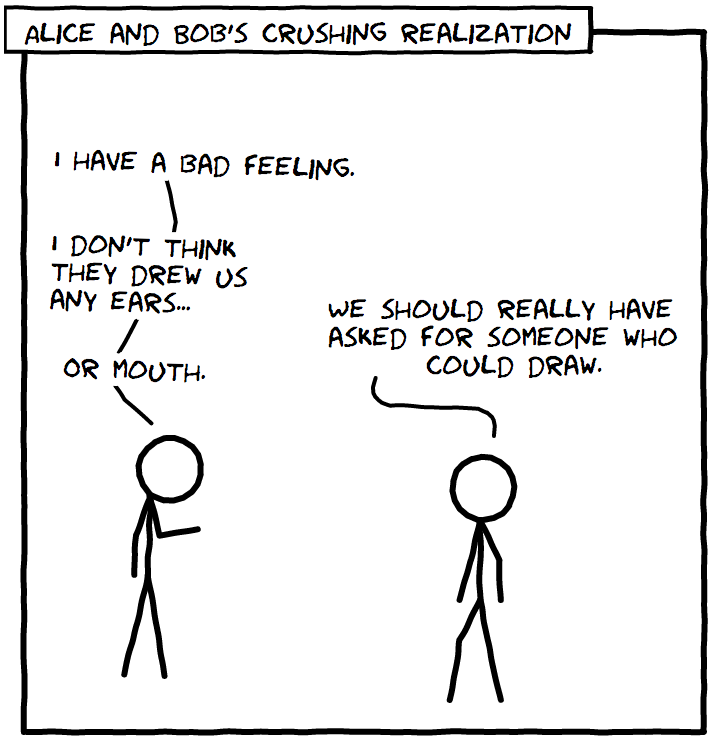
\includegraphics[width=0.5\textwidth]{chapter2/fig-alicebob}
  \caption{Communicating has been somewhat hard for Alice and Bob lately.}
\end{figure}

Extending the framework of Blais, Brody, and Matulef~\cite{BBM:12}, we show a simple way of reducing (private-coin) $\SMP$ problems to distribution testing problems. This foregoing methodology allows us to prove new distribution testing lower bounds, as well as to provide simpler proofs of known lower bounds for problems such as testing uniformity, monotonicity, and $k$-modality (see~\cref{sec:other}). 

Our main result is a characterization of the sample complexity of the distribution identity testing problem in terms of a key operator in the study of interpolation spaces, which arises naturally from our reduction and for which we are able to provide an intuitive interpretation. Recall that in this problem, the goal is to determine whether a distribution $\q$ over domain $\Omega$ (denoted $\q\in\distribs{\Omega}$) is identical to a fixed distribution $\p$; that is, given a full description of $\p\in\distribs{\Omega}$, we ask how many independent samples from $\q$ are needed to decide whether $\q=\p$, or whether $\q$ is $\eps$-far in $\lp[1]$-distance from $\p$.\footnote{Note that this is in fact a family of massively parameterized properties $\{\Pi_p\}_{p\in\distribs{\Omega}}$, where $\Pi_p$ is the property of being identical to $\p$. See~\cite{Newman:10} for an excellent survey concerning massively parameterized properties.}

% \newcommand{\pb}[2]{\parbox[c][][c]{#1}{\strut#2\strut}}
  \begin{table}[ht]\centering\small
    \begin{adjustwidth}{-.5in}{-.5in}\centering
    \def\arraystretch{1.5}   \begin{tabular}{@{}|l|c|c|@{}}\hline
    { \bf Property }& \textbf{Our results} & \bf Previous bounds\\\hline
    {Uniformity}  & $\tildeOmega{\sqrt{n}}$ 
                 & {$\bigTheta{\sqrt{n}}$ \cite{GRexp:00,Paninski:08}} \\\hline
     {Identity to $\p$}  & {$\bigOmega{\kf{\p}^{-1}(1-\eps)}, \bigO{\kf{\p}^{-1}(1-c\cdot\eps)}$ }
                 & {$\bigOmega{\norm{\p^{-\max}_{\eps}}_{2/3}}, \bigO{\norm{\p^{-\max}_{c'\cdot\eps}}_{2/3}}$ \cite{VV:14}} \\\hline
     {Monotonicity}  & $\tildeOmega{\sqrt{n}}$ 
                 & {$\bigTheta{\sqrt{n}}$ \cite{BKR:04,ADK:15,CDGR:16}} \\\hline
     {$k$-modal}  & $\tildeOmega{\sqrt{n}}$
                 & {$\tildeOmega{\max(\sqrt{n},k)}$ \cite{Canonne:16}} \\\hline
     \pb{42mm}{Log-concavity, Monotone Hazard Rate}  & $\tildeOmega{\sqrt{n}}$ 
                 & {$\bigTheta{\sqrt{n}}$ \cite{ADK:15,CDGR:16}} \\\hline
     \pb{42mm}{Binomial, Poisson Binomial}  & $\tildeOmega{{n}^{1/4}}$ 
                 & {$\bigTheta{{n}^{1/4}}$~(\cite{AD:15,CDGR:16}} \\\hline
     \pb{42mm}{Symmetric sparse support}  & $\tildeOmega{\sqrt{n}}$ 
                 & \cellcolor{gray!25}\\\hline
      \pb{42mm}{Junta distributions ($\PCOND$ model)}  & $\bigOmega{k}$ 
                 & \cellcolor{gray!25}\\\hline
  \end{tabular}
  \end{adjustwidth}
    \caption{\label{fig:table:secommunication:results} Summary of results. All the bounds are stated for constant proximity parameter $\eps$.}
  \end{table}
 
In a recent and influential work, Valiant and Valiant~\cite{VV:14} showed that the sample complexity of the foregoing question is closely related to the $\lp[2/3]$-quasinorm of $\p$, defined as $\norm{\p}_{2/3} = \big(\sum_{\omega \in \Omega} \abs{\p(\omega)}^{2/3}\big)^{3/2}$. That is, viewing a distribution $\p \in\distribs{\Omega}$ as an $\abs{\Omega}$-dimensional vector of probabilities, let $\p_{-\eps}^{-\max}$ be the vector obtained from $\p$ by zeroing out the largest entry as well as the set of smallest entries summing to $\eps$ (note that $\p_{-\eps}^{-\max}$ is no longer a probability distribution). Valiant and Valiant gave an $\eps$-tester\footnote{Throughout the introduction, we fix $\eps$ to be small constant and refer to a tester with respect to proximity parameter $\eps$ as an \emph{$\eps$-tester}.}{} for testing identity to $\p$ with sample complexity $O\big({\norm{\p_{-c \eps}^{-\max}}_{2/3}}\big)$, where $c>0$ is a universal constant, and complemented this result with a lower bound of $\Omega\big({\norm{\p_{-\eps}^{-\max}}_{2/3}}\big)$.\footnote{We remark that for certain $\p$'s, the asymptotic behavior of $\bigO{\norm{\p_{-c\eps}^{-\max}}_{2/3}}$ strongly depends on the constant $c$, and so it cannot be omitted from the expression. We further remark that this result was referred to by Valiant and Valiant  as ``instance-optimal identity testing'' as the resulting bounds are phrased as a function of the distribution $\p$ itself -- instead of the standard parameter which is the domain size $n$.}

In this work, using our new methodology, we show alternative and similarly tight bounds on the complexity of identity testing, in terms of a more intuitive measure (as we discuss below) and using simpler arguments. Specifically, we prove that the sample complexity is essentially determined by a fundamental quantity in the theory of interpolation of Banach spaces, known as Peetre's \emph{$K$-functional}. Formally, for a distribution $\p\in\distribs{\Omega}$, the $K$-functional between $\lp[1]$ and $\lp[2]$ spaces is the operator defined for $t>0$ by
\begin{equation*}
    \kf{\p}(t) = \inf_{\p'+ \p''=\p} \normone{\p'} + t\normtwo{\p''}.
\end{equation*}

This operator can be thought of as an interpolation norm between the $\lp[1]$ and $\lp[2]$ norms of the distribution $\p$ (controlled by the parameter $t$), naturally inducing a partition of $\p$ into two sub-distributions: $\p'$, which consists of ``heavy hitters'' in $\lp[1]$-norm, and $\p''$, which has a bounded $\lp[2]$-norm. Indeed, the approach of isolating elements with large mass and testing in $\lp[2]$-norm seems inherent to the problem of identity testing, and is the core component of both early works~\cite{GRexp:00,BFFKRW:01} and more recent ones~\cite{DKN:15,DK:16,Gol:16}. As a further connection to the identity testing question, we provide an easily interpretable proxy for this measure $\kf{\p}$, showing that the $K$-functional between the $\lp[1]$ and $\lp[2]$ norms of the distribution $\p$ is closely related to the size of the effective support of $\p$, which is the number of supported elements that constitute the vast majority of the mass of $\p$; that is, we say that $\p$ has \emph{$\eps$-effective support} of size $T$ if $1- O(\eps)$ of the mass of $\p$ is concentrated on $T$ elements (see~\cref{sec:overview:ub} for details).

Having defined the $K$-functional, we can proceed to state the lower bound we derive for the problem.\footnote{As stated, this result is a slight strengthening of our communication complexity reduction, which yields a lower bound of $\bigOmega{\kf{\p}^{-1}(1-2\eps)/\log n}$. This strengthening is described in~\cref{sec:id:lb}.}
\begin{theorem}[Informally stated]
\label{introthm:1}
Any $\eps$-tester of identity to $\p\in\distribs{\Omega}$ must have sample complexity $\bigOmega{\kf{\p}^{-1}(1-2\eps)}$.
\end{theorem}
\noindent 
In particular, straightforward calculations show that for the uniform distribution we obtain a tight lower bound of $\bigOmega{\sqrt{n}}$, and for the Binomial distribution we obtain a tight lower bound of $\bigOmega{n^{1/4}}$.

To show that tightness of the lower bound above, we complement it with a nearly matching upper bound, also expressed in terms of the $K$-functional.
\begin{theorem}[Informally stated]
\label{introthm:2}
There exist an absolute constant $c>0$ and an $\eps$-tester of identity to $\p\in\distribs{\Omega}$ that uses $\bigO{\kf{\p}^{-1}(1-c\eps)}$ samples.\footnote{Similarly to the~\cite{VV:14} bound, for certain $\p$'s, the asymptotic behavior of $\bigO{\kf{\p}^{-1}(1-2\eps)}$ depends on the constant $c$, and so it cannot be omitted from the expression.}
\end{theorem}
\noindent We remark that for some distributions the bounds in Theorems~\ref{introthm:1}~and~\ref{introthm:2} are tighter than the bounds in \cite{VV:14}, whereas for other distributions it is the other way around (see discussion in Section~\ref{sec:kfunctional}).

In the following section, we provide an overview of our new methodology as well as the proofs for the above theorems. We also further discuss the interpretability of the $K$-functional and show its close connection to the effective support size. We conclude this section by outlining a couple of extensions of our methodology.

\subparagraph{Dealing with sub-constant values of the proximity parameter.} Similarly to the communication complexity methodology for proving property testing lower bounds~\cite{BBM:12}, our method inherently excels in the regime of \emph{constant} values of the proximity parameter $\eps$. Therefore, in this work we indeed focus on the constant proximity regime. However, in~\cref{sec:eps_dep} we demonstrate how to obtain lower bounds that asymptotically increase as $\eps$ tends to zero, via an extension of our general reduction.


\subparagraph{Extending the methodology to testing with conditional samples.} Testers with sample access are by far the most commonly studied algorithms for distribution testing. However, many scenarios that arise both in theory and practice are not  fully captured by this model. In a recent line of works~\cite{CFGM:13,CRS:15,ACK:14,FJOPS:15,FLV:16}, testers with access to \emph{conditional} samples were considered, addressing situations in which one can control the samples that are obtained by requesting samples conditioned on membership on subsets of the domain. In~\cref{sec:extensions}, we give an example showing that it is possible to extend our methodology to obtain lower bounds in the conditional sampling model.

\subsubsection{Organization}
We first give a technical overview in~\cref{sec:technical_overview}, demonstrating the new methodology and presenting our bounds on identity testing. %\cref{sec:prelim} then provides the required preliminaries for the main technical sections. 
In~\cref{sec:methodology} we formally state and analyze the $\SMP$ reduction methodology for proving distribution testing lower bounds. In~\cref{sec:uniformity:communication}, we instantiate the basic reduction, obtaining a lower bound on uniformity testing, and in~\cref{sec:eps_dep} show how to extend the methodology to deal with sub-constant values of the proximity parameter. (We stress that~\cref{sec:eps_dep} is \emph{not} a prerequisite for the rest of the sections, and can be skipped at the reader's convenience.) In~\cref{sec:kfunctional} we provide an exposition to the $K$-functional and generalize inequalities that we shall need for the following sections. \cref{sec:instanceoptimal:identity} then contains the proofs of both lower and upper bounds on the problem of identity testing, in terms of the $K$-functional. In~\cref{sec:other}, we demonstrate how to easily obtain lower bounds for other distribution testing problems. Finally, in~\cref{sec:extensions} we discuss extensions to our methodology; specifically, we explain how to obtain lower bounds in various metrics, and show a reduction from communication complexity to distribution testing in the conditional sampling model.

%%%%%%%%%%%%%%%%%%%%%%%%%%%%%%%%%%%%%%%%%%%%%%%%%%%%%%%%%%%%%%%%%%%%%%%%%%%%%%%%%%%%%%%%%%%%%%%%%%%%%%%%%%%%%%%%%%%%%%%%%%%%%%%%%%%%%%%%%%%%%%%%%%%%%%%
\subsection{Technical Overview}
\label{sec:technical_overview}
In this section we provide an overview of the proof of our main result, which consists of new lower and upper bounds on the sample complexity of testing identity to a given distribution, expressed in terms of an intuitive, easily interpretable measure. To do so, we first introduce the key component of this proof, the methodology for proving lower bounds on distribution testing problems via reductions from SMP communication complexity. We then explain how the relation to the theory of interpolation spaces and the so-called $K$-functional naturally arises when applying this methodology to the identity testing problem.

 For the sake of simplicity, throughout the overview we fix the domain $\Omega = [n]$ and fix the proximity parameter $\eps$ to be a small constant. We begin in~\cref{sec:uniformity_overview} by describing a simple ``vanilla'' reduction for showing an $\tildeOmega{\sqrt{n}}$ lower bound on the complexity of testing that a distribution is uniform. Then, in~\cref{sec:overview:lb} we extend the foregoing approach to obtain a new lower bound on the problem of testing identity to a fixed distribution. This lower bound depends on the best rate obtainable by a special type of error-correcting codes, which we call \emph{$\p$-weighted codes}. In~\cref{sec:overview:detour}, we show how to relate the construction of such codes to concentration of measure inequalities for weighted sums of Rademacher random variables; furthermore, we discuss how the use of the \emph{$K$-functional}, an interpolation norm between $\lp[1]$ and $\lp[2]$ spaces, leads to stronger concentration inequalities than the ones derived by Chernoff bounds or the central limit theorem. Finally, in~\cref{sec:overview:ub} we establish nearly matching upper bounds for testing distribution identity in terms of this $K$-functional, using a proxy known as the $Q$-norm. We then infer that the sample complexity of testing identity to a distribution $\p$ is roughly determined by the size of the \emph{effective support} of $\p$ (which is, loosely speaking, the number of supported elements which together account for the vast majority of the mass of $\p$).

\subsubsection{Warmup: Uniformity Testing.} 
\label{sec:uniformity_overview}
Consider the problem of testing whether a distribution $\q\in\distribs{[n]}$ is the \emph{uniform distribution}; that is, how many (independent) samples from $\q$ are needed to decide whether $\q$ is the uniform distribution over $[n]$, or whether $\q$ is $\eps$-far in $\lp[1]$-distance from it. We reduce the SMP communication complexity problem of \emph{equality} to the distribution testing problem of uniformity testing.

 Recall that in a private-coin SMP protocol for equality, Alice and Bob are given strings $x,y \in \bitset^k$ (respectively), and each of the players is allowed to send a message to a referee (which depends on the player's input and private randomness) who is then required to decide whether $x=y$ by only looking at the players' messages and flipping coins.
 
 \begin{figure}[ht!]
  \centering
  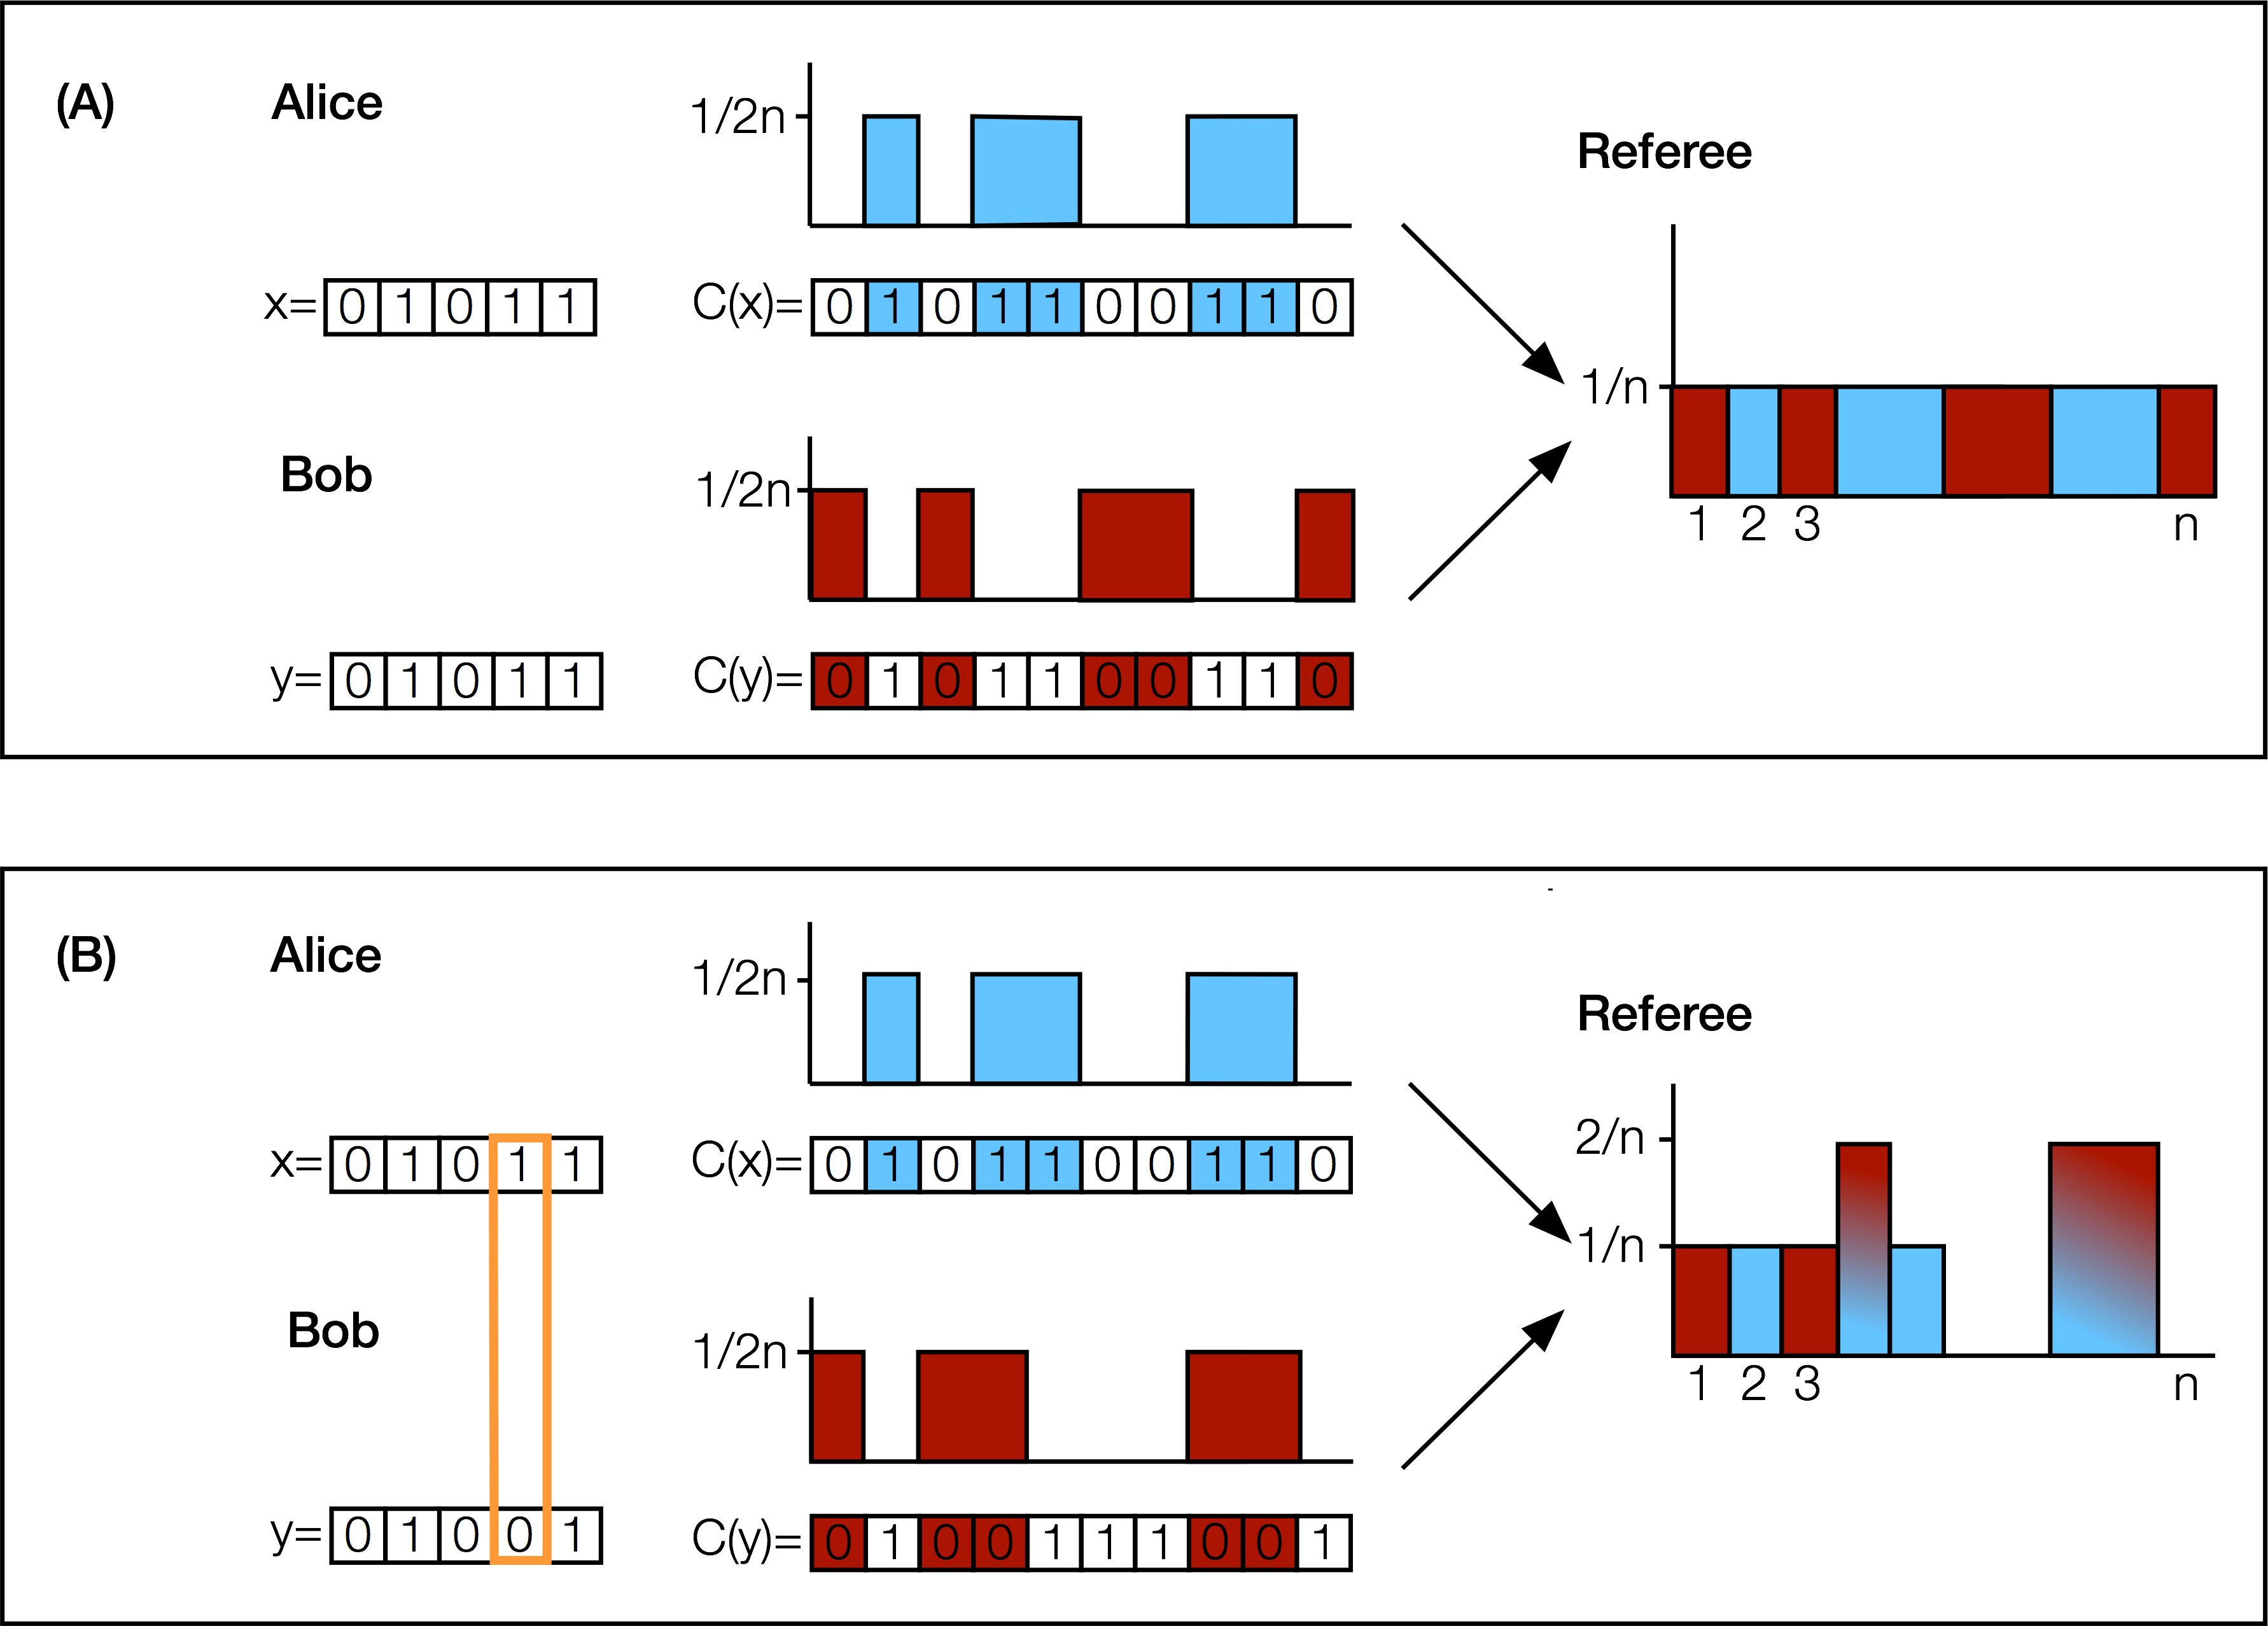
\includegraphics[scale=0.8]{chapter2/img_uniformity.png}
  \caption{{The reduction from equality in the SMP model to uniformity testing of distributions.} In (A) we see that the uniform distribution is obtained when $x=y$, whereas in (B) we see that when $x \neq y$, we obtain a distribution that is ``far'' from uniform.}
  \label{fig:uniformity}
\end{figure}

The reduction is as follows. Assume there exists a uniformity tester with sample complexity $s$. Each of the players encodes its input string via a balanced asymptotically good code $C$ (that is, $C\colon\bitset^k \to \bitset^n$ is an error-correcting code with constant rate and relative distance $\delta = \Omega(1)$, which satisfies the property that each codeword of $C$ contains the same number of $0$'s and $1$'s). Denote by $A \subset [n]$ the locations in which $C(x)$ takes the value $1$ (i.e., $A = \setOfSuchThat{ i\in[n] }{ C(x)_i = 1 }$), and denote by $B \subset [n]$ the locations in which $C(y)$ takes the value $0$ (i.e., $B = \setOfSuchThat{ i\in[n] }{ C(y)_i = 0 }$). Alice and Bob each send $\bigO{s}$ uniformly distributed samples from $A$ and $B$, respectively. Finally, the referee invokes the uniformity tester with respect to the distribution $\q= \left( \uniform_{A}+ \uniform_{B} \right)/2$, emulating each draw from $\q$ by tossing a random coin and deciding accordingly whether to use a sample by Alice or Bob. See~\cref{fig:uniformity}.

The idea is that if $x=y$, then $C(x)=C(y)$, and so $A$ and $B$ are a \emph{partition} of the set $[n]$. Furthermore, since $\abs{C(x)} = \abs{C(y)} = n/2$, this is a equipartition. Now, since Alice and Bob send uniform samples from an equipartition of $[n]$, the distribution $\q$ that the referee emulates is in fact the uniform distribution over $[n]$, and so the uniformity tester will accept. On the other hand, if $x\neq y$, then $C(x)$ and $C(y)$ disagree on a constant fraction of the domain. Thus, $A$ and $B$ intersect on $\delta/2$ elements, as well as do not cover $\delta/2$. Therefore $\q$ is uniform on a $(1-\delta)$-fraction of the domain, unsupported on a $(\delta/2)$-fraction of the domain, and has ``double'' weight $2/n$ on the remaining $(\delta/2)$-fraction. In particular, since $\delta = \bigOmega{1}$, the emulated distribution $\q$ is $\bigOmega{1}$-far (in $\lp[1]$-distance) from uniform, and it will be rejected by the uniformity tester.

As each sample sent by either Alice or Bob was encoded with $\bigO{\log n}$ bits, the above constitutes an SMP protocol for equality with communication complexity $O(s \log(n))$.  Yet it is well known~\cite{newman1996public} that the players must communicate $\Omega(\sqrt{k})$ bits to solve this problem (see~\cref{sec:methodology}), and so we deduce that $s = \Omega(\sqrt{k}/\log(n)) = \tilde\Omega(\sqrt{n})$.

\subsubsection{Revisiting Distribution Identity Testing: A New Lower Bound}
\label{sec:overview:lb}
Next, consider the problem of testing whether a distribution $\q\in\distribs{[n]}$ is identical to a fixed distribution $\p$, provided as a (massive) parameter; that is, given a full description of $\p\in\distribs{[n]}$, we ask how many independent samples from $\q$ are needed to decide whether $\q=\p$, or whether $\q$ is $\eps$-far in $\lp[1]$-distance from $\p$. As mentioned earlier, Valiant and Valiant~\cite{VV:14} established both upper and lower bounds on this problem, involving the $\lp[2/3]$-quasinorm of $\p$. We revisit this question, and show different -- and more interpretable -- upper and lower bounds. First, by applying our new communication complexity methodology to the distribution identity problem, we obtain a simple lower bound expressed in terms of a new parameter, which is closely related to the \emph{effective support size} of $\p$.

Consider any fixed $\p\in\distribs{[n]}$. As a first idea, it is tempting to reduce equality in the SMP model to testing identity to $\p$ by following the uniformity reduction described in~\cref{sec:uniformity_overview}, only instead of having Alice and Bob send \emph{uniform} samples from $A$ and $B$, respectively, we have them send samples from $\p$ \emph{conditioned} on membership in $A$ and $B$ respectively. That is, as before Alice and Bob encode their inputs $x$ and $y$ via a balanced, asymptotically good code $C$ to obtain the sets $A = \setOfSuchThat{ i\in[n] }{ C(x)_i = 1 }$ and $B = \setOfSuchThat{ i\in[n] }{ C(y)_i = 0 }$, which partition $[n]$ if $x=y$, and intersect on $\bigOmega{n}$ elements (as well as fail to cover $\bigOmega{n}$ elements of $[n]$) if $x \neq y$. Only now, Alice sends samples independently drawn from $\p|_A$, i.e., $\p$ conditioned on the samples belonging to $A$, and Bob sends samples independently drawn from $\p|_B$, i.e., $\p$ conditioned on the samples belonging to $B$; and the referee emulates the distribution $\q = (\p|_A + \p|_B)/2$.

However, two problems arise in the foregoing approach. The first is that while indeed when $x=y$ the reduction induces an equipartition $A,B$ of the domain, the resulting weights $\p(A)$ and $\p(B)$ in the mixture may still be dramatically different, in which case the referee will need much more samples from one of the parties to emulate $\p$. The second is a bit more subtle, and has to do with the fact that the properties of this partitioning are with respect to the \emph{size} of the symmetric difference $A\Delta B$, while really we are concerned about its \emph{mass} under the emulated distribution $\q$ (and although both are proportional to each other in the case of the uniform distribution, for general $\p$ we have no such guarantee). Namely, when $x \neq y$ the domain elements which are responsible for the  distance from $\p$ (that is, the elements which are covered by both parties ($A\cap B$) and by neither of the parties ($[n] \setminus (A\cup B)$) may only have a small mass according to $\p$, and thus the emulated distribution $\q$ will not be sufficiently far from $\p$. A natural attempt to address these two problems would be to preprocess $\p$ by discarding its light elements, focusing only on the part of the domain where $\p$ puts enough mass pointwise; yet this approach can also be shown to fail, as in this case the reduction may still not generate enough distance.\footnote{In more detail, this approach would consider the distribution $\p'$ obtained by iteratively removing the lightest elements of $\p$ until a total of $\eps$ probability mass was removed. This way, every element $i$ in the support of $\p'$ is guaranteed to have mass $\p'_i \geq \eps/n$: this implies that the weights $\p'(A)$ and $\p'(B)$ are proportional, and that each element that is either covered by both parties or not covered at all will contribute $\eps/n$ to the distance from $\p'$. However, the total distance of $\q$ from $\p$ would only be $\bigOmega{|\supp{\p'}| \cdot \eps/n}$; and this only suffices if $\p$ and $\p'$ have comparable support size, i.e. $|\supp{\p}| = \bigO{|\supp{\p'}|}$.}

Instead, we take a different route. The key idea is to consider a new type of codes, which we call \emph{$\p$-weighted codes}, which will allow us to circumvent the second obstacle. These are code whose distance guarantee is weighted according to the distribution $\p$; that is, instead of requiring that every two codewords $c,c'$ in a code $C$ satisfy $\dist{x}{y} \eqdef \sum_{i=1}^{n} \abs{ x_i - y_i } \geq \delta$, we consider a code $C_p\colon \bitset^k \to \bitset^n$ such that every $c,c' \in C_p$ satisfy
\[
    \pdist[\p]{x}{y} \eqdef \sum_{i=1}^{n} \p(i)\cdot\abs{ x_i - y_i } \geq \delta.
\]
Furthermore, to handle the first issue, we adapt the ``balance'' property accordingly, requiring that each codeword be balanced according to $\p$, that is, every $c \in C_p$ satisfies $\sum_{i=1}^{n} \p(i)\cdot c_i = 1/2$.

It is straightforward to see that if we invoke the above reduction while letting the parties encode their inputs via a balance $\p$-weighted code $C_p$, then both of the aforementioned problems are resolved; that is, by the $\p$-balance property the weights $\p(A)$ and $\p(B)$ are equal, and by the $\p$-distance of $C_p$ we obtain that for $x \neq y$ the distribution $\q = (\p_A + \p_B)/2$ is $\Omega(1)$-far from $\p$. Hence we obtain a lower bound of $\bigOmega{ \sqrt{k}/\log(n) }$ on the query complexity of testing identity to $\p$. To complete the argument, it remains to construct such codes, and determine what the best rate $k/n$ that can be obtained by $\p$-weighted codes is.

\subsubsection{Detour: $\p$-weighted Codes, Peetre's $K$-functional, and beating the CLT}
\label{sec:overview:detour}
The discussion of previous section left us with the task of constructing high-rate $\p$-weighted codes. Note that unlike standard (uniformly weighted) codes, for which we can easily obtain constant rate, there exist some $\p$'s for which high rate is impossible (for example, if $\p\in\distribs{[n]}$ is only supported on one element, we can only obtain rate $1/n$). In particular, by the sphere packing bound, every $\p$-weighted code $C\colon\bitset^k \to\bitset^n$ with distance $\delta$  must satisfy
\[
      \underbrace{2^k}_{\#\text{codewords}} \leq \frac{2^n}{\operatorname{Vol}_{\mathbb{F}_2^n,\pdistfunc[\p]}(\delta/2) },
\]
where $\operatorname{Vol}_{\mathbb{F}_2^n,\pdistfunc[\p]}(r)$ is the volume of the $\p$-ball of radius $r$ in the $n$-dimensional hypercube, given by
\[
 \operatorname{Vol}_{\mathbb{F}_2^n,\pdistfunc[\p]}(r) 
    \eqdef \abs{ \setOfSuchThat{w\in \mathbb{F}_2^n }{\sum_{i=1}^{n} \p_i\cdot w_i \leq r } }.
\]
Hence, we must have $k \leq n - \log \operatorname{Vol}_{\mathbb{F}_2^n,\pdistfunc[\p]}(\delta/2)$.

 In~\cref{sec:id:lb:cc} we show that there exist (roughly) balanced $\p$-weighted codes with nearly-optimal rate,\footnote{We remark that since these codes are not perfectly $\p$-balanced, a minor modification to the reduction needs to be done. See~\cref{sec:id:lb:cc} for details.} and so it remains to determine the volume of the $\p$-ball of radius $\eps$ in the $n$-dimensional hypercube, where recall that $\eps$ is the proximity parameter of the test. To this end, it will be convenient to represent this quantity as a concentration inequality of sums of weighted Rademacher random variables, as follows
   \begin{equation}
   \label{eq:Vol:overview}
    \operatorname{Vol}_{\mathbb{F}_2^n,\pdistfunc[\p]}(\eps)
        = 2^n \probaDistrOf{Y \sim \bitset^n }{ \sum_{i=1}^n \p_i Y_i \leq \eps } 
        = 2^n \probaDistrOf{X \sim \{-1,1\}^n }{ \sum_{i=1}^n \p_i X_i \geq 1-2\eps}. 
  \end{equation}
    Applying standard tail bounds derived from the central limit theorem (CLT), we have that
   \begin{equation}
   \label{eq:CLT}
 \probaDistrOf{X \sim \{-1,1\}^n }{ \sum_{i=1}^n \p_i X_i \geq 1-2\eps} \le e^{\frac{-(1-2\eps)^2}{2\normtwo{\p}^2}},
  \end{equation}
  and so we can obtain a $\p$-weighted code $C_p\colon\bitset^k \to \bitset^n$ with dimension $k = O(1/\normtwo{\p}^2)$, which in turn, by the reduction described in~\cref{sec:overview:lb}, implies a lower bound of $\bigOmega{1/(\normtwo{\p} \cdot \log(n))}$ on the complexity of testing identity to $\p$.
  
  Unfortunately, the above lower bound is not as strong as hoped, and in particular, far weaker than the $\norm{\p^{-\max}_{-\eps}}_{2/3}$ bound of~\cite{VV:14}.\footnote{For example, fix $\alpha \in (0,1)$, and consider the distribution $\p\in\distribs{[n]}$ in which $n/2$ elements are of mass $1/n$, and $n^{\alpha}/2$ elements are of mass $1/n^{\alpha}$. It is straightforward to verify that $\normtwo{\p}^{-1} = \bigTheta{(\sqrt{n})^{\alpha}}$, whereas $\norm{\p}_{2/3} = \bigTheta{\sqrt{n}}$. (Intuitively, this is because the $\lp[2]$-norm is mostly determined by the few heavy elements, whereas the $\lp[2/3]$-quasinorm is mostly determined by the numerous light elements.)} Indeed, it turns out that the CLT-based bound in~\cref{eq:CLT} is only tight for distributions satisfying $\norminf{\p} = O(\normtwo{\p}^2)$, and is in general too crude for our purposes.
   Instead, we look for stronger concentration of measure inequalities that ``beat'' the CLT. To this end, we shall use powerful tools from the theory of interpolation spaces. Specifically, we consider Peetre's \emph{$K$-functional} between $\lp[1]$ and $\lp[2]$ spaces. Loosely speaking, this is the operator defined for $t>0$ by
\begin{equation*}
    \kf{\p}(t) = \inf_{\p'+ \p'' =\p} \normone{\p'} + t\normtwo{\p''}.\footnotemark
\end{equation*}
\footnotetext{Interestingly, Holmstedt~\cite{Holm:70} showed that the infimum is \emph{approximately} obtained by partitioning $\p = (\p',\p'')$ such that $\p'$ consists of the heaviest $t^2$ coordinates of $\p$ and $\p''$ consists of the rest (for more detail, see~\cref{theo:bounds:kf}).}

This $K$-functional can be thought of as an interpolation norm between the $\lp[1]$ and $\lp[2]$ norms of the distribution $\p$ (and accordingly, for any fixed $t$ it defines a norm on the space $\lp[1]+\lp[2]$). In particular, note that for large values of $t$ the function $\kf{\p}(t)$ is close to $\normone{\p}$, whereas for small values of $t$ it will behave like $t\normtwo{\p}$.

The foregoing connection is due to Montgomery-Smith~\cite{MS:90}, who established the following concentration of measure inequality for weighted sums of Rademacher random variables,
\begin{equation}
\label{eq:Mont:overview}
  \probaOf{ \sum_{i=1}^n \p_i X_i \geq \kf{\p}(t) } \leq e^{-\frac{t^2}{2} }.
\end{equation}

Furthermore, he proved that this concentration bound is essentially tight (see~\cref{sec:kfunctional} for a precise statement). Plugging~\eqref{eq:Mont:overview} into~\eqref{eq:Vol:overview}, we obtain a lower bound of $\Omega(\kf{\p}^{-1}(1-2\eps)/\log(n))$ on the complexity of testing identity to $\p$.

To understand and complement this result, we describe in the next subsection a nearly tight upper bound for this problem, also expressed in terms of this $K$-functional; implying that this unexpected connection is in fact not a coincidence, but instead capturing an intrinsic aspect of the identity testing question. We also give a natural interpretation of this bound, showing that the size of the \emph{effective support} of $\p$ (roughly, the number of supported elements that constitute the vast majority of the mass of $\p$) is a good proxy for this parameter $\kf{\p}^{-1}(1-2\eps)$ -- and thus for the complexity of testing identity to $\p$.

\subsubsection{Using the $Q$-norm Proxy to Obtain an Upper Bound}
\label{sec:overview:ub}
To the end of obtaining an upper bound on the sample complexity of testing identity to $\p$, in terms of the $K$-functional, it will actually be convenient to look at a related quantity, known as the \emph{$Q$-norm}~\cite{MS:90}. At a high-level, the $Q$-norm of a distribution $\p$, for a given parameter $T\in\N$, is the maximum one can reach by partitioning the domain of $\p$ into $T$ sets and taking the sum of the $\lp[2]$ norms of these $T$ subvectors. That is
 \[
    \norm{\p}_{Q(T)} \eqdef \sup \setOfSuchThat{ \sum_{j=1}^T \left( \sum_{i\in A_j} \p_i^2 \right)^{1/2} }{ (A_j)_{1\leq j\leq T} \text{ partition of } \N }.
  \]

Astashkin~\cite{Astashkin:2010}, following up Montgomery-Smith~\cite{MS:90}, showed that the $Q$-norm constitutes a good approximation of $K$-functional, by proving that
  \begin{equation*}
    \norm{\p}_{Q(t^2)} \leq \kf{\p}(t) \leq \sqrt{2}\norm{\p}_{Q(t^2)}.
  \end{equation*}
In~\cref{sec:kfunctional} we further generalize this claim and show it is possible to get a tradeoff in the upper bound; specifically, we prove that
$\kf{\p}(t) \leq \norm{\p}_{Q(2t^2)}$. Thus, it suffices to prove an upper bound on distribution identity testing in terms of the $Q$-norm.

From an algorithmic point of view, it is not immediately clear that switching to this $Q$-norm is of any help. However, we will argue that this value captures -- in a very quantitative sense -- the notion of the \emph{sparsity} of $\p$. As a first step, observe that if $\norm{\p}_{Q(T)} = 1$, then the distribution $\p$ is supported on at most $T$ elements. To see this, denote by $\p_{A_j}$ the restriction of the sequence $\p$ to the indices in $A_j$, and note that if $\norm{\p}_{Q(T)} \eqdef \sum_{j=1}^T \normtwo{ \p_{A_j} }=1$, then  by the monotonicity of $\lp[p]$ norms and since $\sum_{j=1}^T \normone{ \p_{A_j} } = \normone{\p}=1$ we have that
\[
      \sum_{j=1}^T (\underbrace{ \normone{ \p_{A_j} } - \normtwo{ \p_{A_j} } }_{\geq 0}) = 0,
\]
which implies that $\normone{ \p_{A_j} } = \normtwo{ \p_{A_j} }$ for all $j\in[T]$.

Now, it turns out that it is possible to obtain a \emph{robust} version of the foregoing observation, yielding a sparsity lemma that, roughly speaking, shows thats if $\norm{\p}_{Q(T)} \geq 1-\eps$, then $1- O(\eps)$ of the mass of $\p$ is concentrated on $T$ elements: in this case we say that $\p$ has \emph{$O(\eps)$-effective support} of size $T$. (See \cref{lemma:ub:key} for precise statement of the sparsity lemma.)

 This property of the $Q$-norm suggests the following natural test for identity to a distribution $\p$: Simply fix $T$ such that  $\norm{\p}_{Q(T)} = 1-\eps$, and apply one of the standard procedures for testing identity to a distribution with support size $T$, which require $O(\sqrt{T})$ samples. But by the previous discussion, we have $\norm{\p}_{Q(2t^2)} \geq \kf{\p}(t)$, so that setting $T=2t^2$ for the ``right'' choice of $t=\kf{\p}^{-1}(1-2\eps)$ will translate to an $O(t)$ upper bound -- which is what we were aiming for.
 
%%%%%%%%%%%%%%%%%%%%%%%%%%%%%%%%%%%%%%%%%%%%%%%%%%%%%%%%%%%%%%%%%%%%%%%%%%%%%%%%%%%%%%%%%%%%%%%%%%%%%%%%%%%%%%%%%%%%%%%%%%%%%%%%%%%%%%%%%%%%%%%%%%%%%%%
\subsection{The Methodology: From Communication Complexity to Distribution Testing}\label{sec:methodology}
In this section we adapt the methodology for proving property testing lower bounds via reductions from communication complexity, due to Blais, Brody, and Matulef~\cite{BBM:12}, to the setting of distribution testing.  As observed in~\cite{BBM:12,BMW:11}, to prove lower bounds on the query complexity of \emph{non-adaptive} testers it suffices to reduce from one-sided communication complexity. We show that for distribution testers (which are inherently non-adaptive), it suffices to reduce from the more restricted communication complexity model of \emph{private-coin} simultaneous message passing (SMP).

Recall that a private-coin SMP protocol for a communication complexity predicate $f\colon \bitset^k \times \bitset^k \to \bitset$ consists of three computationally unbounded  parties: Two players (commonly referred to as Alice and Bob), and a Referee. Alice and Bob receive inputs $x,y \in \bitset^k$. Each of the players simultaneously (and independently) sends a message to the referee, based on its input and (private) randomness. The referee is then required to successfully compute $f(x,y)$ with probability at least $2/3$, using its private randomness and the messages received from Alice and Bob. The communication complexity of an SMP protocol is the total number of bits sent by Alice and Bob. The private-coin SMP complexity of $f$, denoted $\SMP(f)$, is the minimum communication complexity of all SMP protocols that solve $f$ with probability at least $2/3$.

Generally, to reduce an SMP problem $f$ to $\eps$-testing a distribution property $\Pi$, Alice and Bob can send  messages $m_A(x,r_A,\eps)$ and $m_B(y,r_B,\eps)$ (respectively) to the Referee, where $r_A$ and $r_B$ are the private random strings of Alice and Bob. Subsequently, the Referee uses the messages $m_A(x,r_A,\eps)$ and $m_A(y,r_B,\eps)$, as well as its own private randomness, to feed the property tester samples from a distribution $\p$ that satisfies the following conditions: (1) \emph{completeness}: if $f(x,y)=1$, then $\p\in \Pi$; and (2) \emph{soundness}: if $f(x,y)=0$, then $\p$ is $\eps$-far from $\Pi$ in $\ell_1$-distance.

We shall focus on a special type of the foregoing reductions, which is particularly convenient to work with and suffices for all of the our lower bounds. Loosely speaking, in these reductions Alice and Bob both send the prover samples from sub-distributions that can be combined by the Referee to obtain samples from a distribution that satisfies the completeness and soundness conditions. The following lemma gives a framework for proving lower bounds based on such reductions.

\begin{lemma}\label{lemma:main:methodology:reduction}
	Let $\eps>0$, and let $\Omega$ be a finite domain of cardinality $n$. Fix a property $\Pi \subseteq \distribs{\Omega}$ and a communication complexity predicate $f\colon \bitset^k \times \bitset^k \to \bitset$. Suppose that there exists a mapping $\p\colon\bitset^k \times \bitset^k \to \distribs{\Omega}$ that satisfies the following conditions.
	\begin{enumerate}
		\item \emph{Decomposability:} For every $x,y\in\bitset^k$, there exist constants $\alpha=\alpha(x), \beta=\beta(y) \in [0,1]$ and distributions $\p_A(x), \p_B(y)$ such that 
		\[
		p(x,y) = \frac{\alpha}{\alpha+\beta}\cdot \p_A(x) + \frac{\beta}{\alpha+\beta}\cdot \p_B(y)
		\] 
		and $\alpha,\beta$ can each be encoded with $\bigO{\log n}$ bits.
		\item \emph{Completeness:} For every $(x,y) = f^{-1}(1)$, it holds that $\p(x,y) \in \Pi$.
		\item \emph{Soundness:} For every $(x,y) = f^{-1}(0)$, it holds that $\p(x,y)$ is $\eps$-far from $\Pi$ in $\ell_1$ distance.
	\end{enumerate}
	Then, every $\eps$-tester for $\Pi$ needs $\bigOmega{\frac{\SMP(f)}{\log(n)}}$ samples.
\end{lemma}

\begin{proof}
Supose there exists an $\eps$-tester for $\Pi$ with sample complexity $s'$; assume without loss of generality that the soundness of the foregoing tester is $5/6$, at the cost of increasing the query complexity to $s=O(s')$. Let $x,y\in\bitset^k$ be the inputs of Alice and Bob (respectively) for the SMP problem. Alice computes the distribution $\p_A(x)$ and the ``decomposability parameter" $\alpha=\alpha(x)$ and sends $6 s$  independent samples from $\p_A(x)$, as well as the parameter $\alpha$. Analogously, Bob computes $\p_B(y)$ and its parameter $\beta=\beta(y)$, and sends $6s$ independent samples from $\p_B(y)$ as well as the parameter $\beta$. Subsequently, the referee generates a sequence of $\q$ independent samples from $\p(x,y)$, where each sample is drawn as follows: with probability $\frac{\alpha}{\alpha+\beta}$ use a (fresh) sample from Alice's samples, and with probability $1-\frac{\alpha}{\alpha+\beta}$ use a (fresh) sample from Bob's samples. Finally the referee feeds the generated samples to the $\eps$-tester for $\Pi$.

By Markov's inequality, the above procedure indeed allows the referee to retrieve, with probability at least $1-\frac{\alpha s}{6 s}\geq\frac{5}{6}$, at least $s$ independent samples from the distribution $\frac{\alpha}{\alpha+\beta}\cdot \p_A(x) + \frac{\beta}{\alpha+\beta}\cdot \p_B(y)$, which equals to $\p(x,y)$, by the decomposability condition. If $(x,y) = f^{-1}(1)$, then by the completeness condition $\p(x,y) \in \Pi$, and so the $\eps$-tester for $\Pi$ is successful with probability at least $\frac56 \cdot \frac 56$. Similarly, if $(x,y) = f^{-1}(0)$, then by the soundness condition $\p(x,y)$ is $\eps$-far from $\Pi$, and so the $\eps$-tester for $\Pi$ is successful with probability at least $\frac56 \cdot \frac 56$. Finally, note that since each one of the samples provided by Alice and Bob requires sending $\log n$ bits, the total communication complexity of the protocol is $12s\log n + \bigO{\log n}$ (the last term from the cost of sending $\alpha,\beta$), hence $s' = \bigOmega{\frac{\SMP(f)}{\log(n)}}$.
\end{proof}

We conclude this section by stating a well-known SMP lower bound on the equality problem. Let $\EQ[k]\colon \bitset^k \times \bitset^k \to \bitset$ be the equality predicate, i.e., $\EQ[k](x,y)=1$ if and only if $x=y$. In this work, we shall frequently use the following (tight) lower bound on the $\EQ[k]$ predicate:
\begin{theorem}[Newman and Szegedy~\cite{newman1996public}]\label{theo:equality:smp:lb}
For every $k\in\N$ it holds that $\SMP(\EQ[k]) =\bigOmega{\sqrt{k}}$.
\end{theorem}
 
%%%%%%%%%%%%%%%%%%%%%%%%%%%%%%%%%%%%%%%%%%%%%%%%%%%%%%%%%%%%%%%%%%%%%%%%%%%%%%%%%%%%%%%%%%%%%%%%%%%%%%%%%%%%%%%%%%%%%%%%%%%%%%%%%%%%%%%%%%%%%%%%%%%%%%%
\subsection{The Basic Reduction: The Case of Uniformity}\label{sec:uniformity:communication}
\begin{theorem}
\label{theo:uniformity:lb}
For any $\eps\in(0,1/2)$ and finite domain $\Omega$, testing that $\p\in \distribs{\Omega}$ is uniform, with respect to proximity parameter $\eps$, requires $\tildeOmega{\sqrt{n}}$ samples, where $n = |\Omega|$.
\end{theorem}
\begin{proof}
Assume there exists a $\q$-query $\eps$-tester for the uniform distribution, with error probability $1/6$. For a sufficiently large $k\in\N$, let $C\colon \bitset^k \to \bitset^n$ be a balanced code as promised by~\cref{lemma:good:balanced:hamming:codes} with distance $\eps$. Namely, there exists an absolute constant $\rho > 0$ such that
\begin{enumerate}[(i)]
  \item $\abs{C(x)} = \frac{n}{2}$ for all $x\in \bitset^k$;
  \item $\dist{C(x)}{C(y)} > \eps$ for all distinct $x,y\in \bitset^k$;
  \item $\frac{k}{n} \geq \rho$.
\end{enumerate}
Given their respective inputs $x,y\in\{0,1\}^k$ from $\EQ[k]$, Alice and Bob separately create inputs $(C(x),C(y))\in\{0,1\}^n\times\{0,1\}^n$, and the corresponding sets $A\eqdef \setOfSuchThat{ i\in[n] }{ C(x)_i=1 }$, $B\eqdef \setOfSuchThat{ i\in[n] }{ C(y)_i =0 }$. We then invoke the general reduction of~\cref{lemma:main:methodology:reduction} as follows: we set $\alpha=\beta=\frac{1}{2}$, and $\p_A(x)\in\distribs{\domain}$ (respectively $\p_B(y)\in\distribs{\domain}$) to be the uniform distribution on the set $A$ (respectively $B$). It is clear that the decomposability condition of the lemma is satisfied for $\p(x,y) = \frac{\alpha}{\alpha+\beta} \cdot \p_A(x)+\frac{\beta}{\alpha+\beta} \cdot \p_B(y) = \frac{1}{2}(\p_A(x)+\p_B(y))$; we thus turn to the second and third conditions.

\begin{description}
  \item[Completeness.] If $(x,y)\in \EQ[k]^{-1}(1)$, then $C(x)=C(y)$ and $A=[n]\setminus B$. This implies that $\p(x,y)$ is indeed the uniform distribution on $[n]$, as desired.
  \item[Soundness.] If $(x,y)\in \EQ[k]^{-1}(0)$, then $\dist{C(x)}{C(y)} > \eps$, and therefore $\dabs{A\triangle \bar{B}} > \eps n$ by construction. Since $\p(x,y)$ assigns mass $2/n$ to each element in $A\cap B=A\setminus \bar{B}$, and mass $0$ to any element in $\bar{A}\cap \bar{B}=\bar{B}\setminus A$, we have $\normone{\p(x,y) - u} = \frac{1}{n}\cdot\dabs{A\triangle \bar{B}} > \eps$; that is, $\p(x,y)$ is \eps-far from uniform.
\end{description}
The desired $\bigOmega{\frac{\sqrt{n}}{\log n}}$ lower bound then immediately follows from~\cref{lemma:main:methodology:reduction} and~\cref{theo:equality:smp:lb}.
\end{proof} 
\subsubsection{Obtaining $\eps$-Dependency}\label{sec:eps_dep}
In this section, we explain how to generalize the reduction from the previous section to obtain some dependence (albeit non optimal) on the distance parameter $\eps$ in the lower bound. This generalization will rely on an extension of the methodology of~\cref{lemma:main:methodology:reduction}: instead of having the referee define the distribution $\p(x,y)$ as a mixture of $\p_A(x)$ and $\p_B(y)$ (namely, $\p(x,y) = \frac{\alpha(x)}{\alpha(x)+\beta(y)}\p_A(x)+\frac{\beta(y)}{\alpha(x)+\beta(y)}\p_B(y)$), he will instead use a (random) combination function $F_\eps$, function of $\eps$ and its private coins only. Given this function, which maps a larger domain of size $m=\bigTheta{n/\eps^2}$ to $[n]$, $\p(x,y)$ will be defined as the mixture
\[
    \p(x,y) = \frac{\alpha(x)}{\alpha(x)+\beta(y)}\p_A(x) \circ F_\eps^{-1} +  \frac{\beta(y)}{\alpha(x)+\beta(y)} \p_B(y) \circ F_\eps^{-1}.
\]
More simply, this allows Alice and Bob to send to the referee samples from their respective distributions on a much larger domain $m \gg n$; the referee, who has on its side chosen how to randomly partition this large domain into only $n$ different ``buckets,'' converts these draws from Alice and Bob into samples from the induced distributions on the $n$ buckets, and takes a mixture of these two distributions instead. By choosing each bucket to chave size roughly $1/\eps^2$, we expect this random ``coarsening'' of Alice and Bob's distributions to yield a distribution at distance only $\Omega(\eps)$ from uniformity (instead of constant distance) in the \no-case; but now letting us get a lower bound on the \emph{original} support size $m$, i.e. $\tildeOmega{\sqrt{n/\eps^2}}$, instead of $\tildeOmega{\sqrt{n}}$ as before.

\begin{theorem}\label{theo:uniformity:eps}
For any $\eps\in(0,1/2)$ and finite domain $\Omega$, testing that $\p\in \distribs{\Omega}$ is uniform, with respect to proximity parameter $\eps$, requires $\tildeOmega{\sqrt{n}/\eps}$ samples, where $n = |\Omega|$.
\end{theorem}
\begin{proofof}{\cref{theo:uniformity:eps}}
We will reduce from $\EQ[k]$, where $k\in\N$ is again assumed big enough (in particular, with regard to $1/\eps^2$). Alice and Bob act as in~\cref{sec:uniformity:communication}, separately creating $(a,b)=(C(x),C(y))\in\{0,1\}^m\times \in\{0,1\}^m$ from their respective inputs $x,y\in \{0,1\}^k$ (where $C\colon \bitset^k \to \bitset^m$ is a balanced code with linear rate and distance $\delta\eqdef 1/3$). As before, they consider the sets $A\eqdef \setOfSuchThat{ i\in[m] }{ C(x)_i=1 }$, $B\eqdef \setOfSuchThat{ i\in[m] }{ C(y)_i=0 }$, set $\alpha=\beta=\frac{1}{2}$, and consider the distributions $\p_A(x),\p_B(y)\in\distribs{[m]}$ which are uniform respectively on $A$ and $B$.

This is where we deviate from the proof of~\cref{theo:uniformity:lb}: indeed, setting $n\eqdef c \eps^2 m$ (where $c>0$ is an absolute constant determined later), the referee will combine the samples from $\p_A(x)$ and $\p_B(y)$ in a different way to emulate a distribution $\p(x,y)\in\distribs{[n]}$ -- that is, with a much smaller support than that of $\p_A(x),\p_B(y)$ (instead of setting $\p(x,y)$ to be, as before, a mixture of the two).

To do so, the referee randomly partitions $[m]$ into $n$ sets $B_1,\dots, B_n$ of equal size $r\eqdef \abs{B_j} = \frac{m}{n} = \frac{1}{c\eps^2}$, $j\in[n]$, by choosing a uniformly random equipartition of $[m]$. He then defines the distribution $\p=\p(x,y)\in\distribs{[n]}$ by $\p(j) = \probaOf{ i \in B_j }$ (where $i\in[m]$ is received from either Alice or Bob). Viewed differently, the random equipartition chosen by the referee induces a mapping $F_\eps\colon [m] \to [n]$ such that $\abs{F^{-1}(j)} = r$ for all $j\in[n]$; and, setting $\p'(x,y) = \frac{1}{2}(\p_A(x)+\p_B(y))\in\distribs{[m]}$, we obtain $\p(x,y)$ as the \emph{coarsening} of $\p'(x,y)$ defined as
\[
    \p(x,y)(j) = \sum_{i\in F_\eps^{-1}(j)} p'(x,y)(i) = p'(x,y)( F_\eps^{-1}(j) ) = \frac{1}{2}\left( \p_A(x)( F_\eps^{-1}(j) ) +\p_B(y)( F_\eps^{-1}(j) ) \right), \qquad j\in [n].
\]
Note furthermore that each sample sent by Alice and Bob (who have no knowledge of the randomly chosen $F_\eps$) can be encoded with $O(\log m) = O(\log\frac{n}{\eps})$ bits.

We then turn to establish the analogue in this generalized reduction of the last two conditions of~\cref{lemma:main:methodology:reduction}, i.e. the completeness and soundness. The former, formally stated below, will be an easy consequence of the previous section.
\begin{claim}\label{claim:eps:uniformity:completeness}
If $x=y$, then $\p(x,y)$ is uniform on $[n]$.
\end{claim}
\begin{proof}
As in the proof of~\cref{theo:uniformity:lb}, in this case the distribution $\p'(x,y) = \frac{1}{2}(\p_A(x)+\p_B(y))\in\distribs{[m]}$ is uniform; since each ``bucket'' $B_j=F_\eps^{-1}(j)$ has the same size, this implies that $\p(x,y)(j) = p'(x,y)( B_j ) = \frac{1}{n}$ for all $j\in[n]$.
\end{proof}

\noindent Establishing the soundness, however, is not as straightforward:
\begin{claim}\label{claim:eps:uniformity:soundness}
If $x\neq y$, then with probability at least $1/100$ (over the choice of the equipartition $(B_1,\dots, B_n)$), $\p(x,y)$ is \eps-far from uniform.
\end{claim}
\begin{proof}
Before delving into the proof, we provide a high-level idea of why this holds. Since the partition was chosen uniformly at random, on expectation each element $j\in[n]$ will have probability $\expect{\p(x,y)(j)} = \expect{\p'(x,y)( B_j )} = \frac{1}{n}$. However, since a constant fraction of elements $i\in[m]$ (before the random partition) has probability mass either $0$ or $2/m$ (as in the proof of~\cref{theo:uniformity:lb}), and each bucket $B_j$ contains $r=1/(c\eps^2)$ many elements chosen uniformly at random, we expect the fluctuations of $\p'(x,y)( B_j )$ around its expectation to be of the order of $\bigOmega{\sqrt{r}/m} = \bigOmega{\eps/n}$ with constant probability, and summing over all $j$'s this will give us the distance $\bigOmega{\eps}$ we want.

To make this argument precise, we assume $x\neq y$, so that $A\triangle \bar{B} > \delta m$; and define $H\eqdef A\cap B,L\eqdef\bar{A}\cap \bar{B}$ (so that $\abs{H}=\abs{L} > \frac{\delta}{2}m$). For any $j\in[n]$, we then let the random variables $H^{(j)}, L^{(j)}$ be the number of ``high'' and ''low'' elements of $[m]$ in the bucket $B_j$, respectively:
\[
H^{(j)} \eqdef \abs{B_j\cap H}, \qquad L^{(j)} \eqdef \abs{B_j\cap L}.
\]
From the definition, we get that $\p=\p(x,y)$ satisfies $\p(j) = \frac{1}{m}\left(2H^{(j)} + (r - H^{(j)} - L^{(j)}\right) = \frac{r}{m} + \frac{H^{(j)} - L^{(j)}}{m}$ for $j\in[n]$. Furthermore, it is easy to see that $\expect{\p(j)} = \frac{r}{m} = \frac{1}{n}$ for all $j\in[n]$, where the expectation is over the choice of the equipartition by the referee.

As previously discussed, we will analyze the deviation from this expectation; more precisely, we want to show that with good probability, a constant fraction of the $j$'s will be such that $\p(j)$ deviates from ${1}/{n}$ by at least an additive $\bigOmega{{\sqrt{r}}/{m}} = {\eps}/{n}$. This anticoncentration guarantee will be a consequence of the Paley--Zygmund inequality (\cref{theo:paley:zigmund}) to $Z^{(j)}\eqdef (H^{(j)} - L^{(j)})^2 \geq 0$; in view of applying it, we need to analyze the first two moments of this random variable.
  \begin{lemma}\label{lemma:eps:uniformity:soundness:anticoncentration}
    For any $j\in[n]$, we have the following. (i) $\expect{(H^{(j)} - L^{(j)})^2} = \delta r \frac{m-r}{m-1}$, and (ii)~$\expect{(H^{(j)} - L^{(j)})^4} = 3(1+o(1)) \delta^2 r^2$.
  \end{lemma}
  \begin{proof}
Fix any $j\in[n]$. We write for convenience $X$ and $Y$ for respectively $H^{(j)}$ and $L^{(j)}$. The distribution of $(X,Y,r-(X-Y))$ is then a \emph{multivariate hypergeometric distribution}~\cite{wiki:hypergeom} with $3$ classes:
\[
(X,Y,r-(X+Y))\sim \operatorname{MultivHypergeom}_3(\underbrace{(\tfrac{1}{2}\delta m,\tfrac{1}{2}\delta m,(1-\delta) m)}_{(K_1,K_2,K_3)}, m, r).
\]
Conditioning on $U\eqdef X+Y$, we have that $\expect{X\mid U}$ follows a hypergeometric distribution, specifically $\expect{X\mid U} \sim \operatorname{Hypergeom}(U, \frac{1}{2} \delta m, \delta m)$. Moreover, $U$ itself is hypergeometrically distributed, with
$U \sim \operatorname{Hypergeom}(r, \delta m, m)$. We can thus write
\[
\expect{(X-Y)^2} = \expect{ \expect{(X-Y)^2\mid U }} = \expect{\expect{(2X-U)^2\mid U }}
\]
and
\[
\expect{(X-Y)^4} = \expect{ \expect{(X-Y)^4\mid U }} = \expect{\expect{(2X-U)^4\mid U }}.
\]

By straightforward, yet tedious, calculations involving the computation of $\expect{(2X-U)^2\mid U }$ and $\expect{(2X-U)^4\mid U }$ (after expanding and using the known moments of the hypergeometric distribution),\footnote{One can also use a formal computation system, e.g. Mathematica:\scriptsize
\begin{verbatim}
 Expectation[ Expectation[(2 X - U)^2, {X \[Distributed] HypergeometricDistribution[U, a*m, 2 a*m]}],
   {U \[Distributed] HypergeometricDistribution[r, 2*a*m, m]}]
 Expectation[ Expectation[(2 X - U)^4, {X \[Distributed] HypergeometricDistribution[U, a*m, 2 a*m]}],
   {U \[Distributed] HypergeometricDistribution[r, 2*a*m, m]}]
\end{verbatim}
}{} we obtain
\begin{align*}
  \expect{(X-Y)^2} &= \delta r \frac{m-r}{m-1} \operatorname*{=}_{m\to\infty} (1+o(1)) \delta r \\
  \expect{(X-Y)^4} &= \frac{(\delta r (r - m) ((-1 + 3\delta (m-1) - m) m + 6 r^2 (\frac{1}{2}\delta m-1) - 6 r m (\frac{1}{2}\delta m-1)))}{(m-3) (m-2) (m-1)} \\
  &\xrightarrow[m\to\infty]{} 3\delta^2 r^2 + (1 - 3\delta) \delta r = 3\delta^2 r^2
\end{align*}
the last equality as $\delta=1/3$.
  \end{proof}
  We can now apply the Paley--Zygmund inequality to $Z^{(j)}$. Doing so, we obtain that for $r \leq \frac{m}{4}$ (with some slack), and any $\theta\in[0,1]$,
  \[
      \probaOf{ \abs{H^{(j)} - L^{(j)}} \geq \theta \sqrt{\frac{1}{2}\delta r} } 
      \geq
      \probaOf{ \abs{H^{(j)} - L^{(j)}} \geq \theta \sqrt{\delta r \frac{m-r}{m-1}} } \geq (1-\theta^2)^2\frac{\expect{(H^{(j)} - L^{(j)})^2}^2}{\expect{(H^{(j)} - L^{(j)})^4}}.
  \]
  By the lemma above, the RHS converges to $\frac{(1-\theta^2)^2}{3}$ when $m\to \infty$, and therefore is at least $\frac{(1-\theta^2)^2}{4}$ for $m$ big enough. We set $\theta \eqdef 1/\sqrt{2}$ to obtain the following: there exists $M\geq 0$ such that
  \begin{equation}\label{eq:eps:uniformity:soundness:pz}
    \probaOf{ \abs{H^{(j)} - L^{(j)}} \geq \sqrt{\frac{\delta r}{4}} } \geq \frac{1}{16}
  \end{equation}
  for every $m\geq M$.
  
  Eq.~\eqref{eq:eps:uniformity:soundness:pz} implies that the number $K$ of \emph{good} indices $j\in[n]$ satisfying $\abs{H^{(j)} - L^{(j)}} \geq \sqrt{\frac{\delta r}{4}}$ is on expectation at least $\frac{n}{16}$, and by an averaging argument\footnote{Applying Markov's inequality: $\probaOf{K < \frac{n}{20}} = \probaOf{n-K > \frac{19n}{20}} \leq \frac{n-\expect{K}}{19n/20} \leq  \frac{15/16}{19/20} = \frac{75}{76}$.}  we get that $K\geq \frac{n}{20}$ with probability at least $\frac{1}{76} > \frac{1}{100}$.
  
  Whenever this happens, the distance from $\p$ to uniform is at least 
  \[
  \sum_{j\text{ \text{good}}} \abs{\p(j) - \frac{1}{n}} = \sum_{j\text{ \text{good}}} \frac{\abs{H^{(j)} - L^{(j)}}}{m} \geq \frac{n}{20}\cdot \frac{\sqrt{\frac{\delta r}{4}}}{m} = \frac{\sqrt{\delta r}}{40} \frac{n}{m} = \frac{\sqrt{c}}{40\sqrt{3}}\eps
  \]
  and choosing $c \geq 4800$ so that $\frac{\sqrt{c}}{40\sqrt{3}} \geq 1$ yields the claim.
\end{proof}

From this lemma, we can complete the reduction: given a tester $\Tester$ for uniformity with query complexity $\q$, we first convert it by standard amplification into a tester $\Tester^\prime$ with failure probability $\delta\eqdef 1/1000$ and sample complexity $\bigO{q}$. The referee can provide samples from the distribution $\p(x,t)$, and on input $\eps$:
\begin{itemize}
  \item If $x=y$, then $\Tester^\prime$ will return \reject with probability at most $1/200$;
  \item If $x\neq y$, then $\Tester^\prime$ will return \reject with probability at least $199/200\cdot 1/100 > 1/200$;
\end{itemize} 
so repeating independently the protocol a constant (fixed in advance) number of times and taking a majority vote enables the referee to solve $\EQ[k]$ with probability at least $2/3$. Since $\bigOmega{\sqrt{k}} = \bigOmega{\sqrt{n/\eps^2}}$ bits of communication are required for this, and each sample sent by Alice or Bob to the referee only requires $\bigTheta{\log \frac{n}{\eps}}$ bits, we get a lower bound of 
\[
    \bigOmega{\frac{\sqrt{n}}{\eps\log \frac{n}{\eps}}} = \tildeOmega{\frac{\sqrt{n}}{\eps}}
\]
on the sample complexity of $\Tester^\prime$, and therefore of $\Tester$.
\end{proofof}
 
%%%%%%%%%%%%%%%%%%%%%%%%%%%%%%%%%%%%%%%%%%%%%%%%%%%%%%%%%%%%%%%%%%%%%%%%%%%%%%%%%%%%%%%%%%%%%%%%%%%%%%%%%%%%%%%%%%%%%%%%%%%%%%%%%%%%%%%%%%%%%%%%%%%%%%%
\subsection{The $K$-Functional: An Unexpected Journey}\label{sec:kfunctional}
A quantity that will play a major role in our results is the \emph{$K$-functional between $\lp[1]$ and $\lp[2]$}, a specific case of the key operator in interpolation theory introduced by Peetre~\cite{Peetre:68}. We start by recalling below the definition and some of its properties, before establishing (for our particular setting) results that will be crucial to us. (For more on the $K$-functional and its use in functional analysis, the reader is referred to~\cite{BennettS:88} and~\cite{Astashkin:2010}.)
\begin{definition}[$K$-functional]\label{def:kfunctional}
Fix any two Banach spaces $(X_0, \norm{\cdot}_0), (X_1, \norm{\cdot}_1)$.
The \emph{$K$-functional} between $X_0$ and $X_1$ is the function $K_{X_0,X_1}\colon (X_0+X_1)\times(0,\infty)\to [0,\infty)$ defined by
\[
    K_{X_0,X_1}(x,t) \eqdef \inf_{\substack{(x_0,x_1)\in X_0\times X_1 \\ x_0+x_1=x}} \norm{x_0}_0 + t\norm{x_1}_1.
\]
For $a\in\lp[1]+\lp[2]$, we denote by $\kf{a}$ the function $t\mapsto K_{\lp[1],\lp[2]}(a,t)$.
\end{definition}

In other terms, as $t$ varies the quantity $\kf{a}(t)$ interpolates between the $\lp[1]$ and $\lp[2]$ norms of the sequence $a$ (and accordingly, for any fixed $t$ it defines a norm on $\lp[1]+\lp[2]$). In particular, note that for large values of $t$ the function $\kf{a}(t)$ is close to $\norm{x}_1$, whereas for small values of $t$ the function $\kf{a}(t)$ is close to $t\norm{x}_2$ (see \cref{coro:properties:kf}). We henceforth focus on the case of $K_{\lp[1],\lp[2]}$, although some of the results mentioned hold for the general setting of arbitrary Banach $X_0,X_1$.

\begin{proposition}[{\cite[Proposition 1.2]{BennettS:88}}]\label{prop:kfunctional:basic}
For any $a\in\lp[1]+\lp[2]$, $\kf{a}$ is continuous, increasing, and concave. Moreover, the function $t\in(0,1)\mapsto \frac{\kf{a}}{t}$ is decreasing.
\end{proposition}

Although no closed-form expression is known for $\kf{a}$, it will be necessary for us to understand its behavior, and therefore seek good upper and lower bounds on its value. We start with the following inequality, due to Holmstedt~\cite{Holm:70}, which, loosely speaking, shows that the infimum in the definition of $\kf{a}(t)$ is \emph{roughly} obtained by partitioning $a = (a_1,a_2)$ such that $a_1$ consists of heaviest $t^2$ coordinates of $a$, and $a_2$ consists of the rest.
\begin{proposition}[{\cite[Proposition 2.2]{Astashkin:2010}}, after {\cite[Theorem 4.2]{Holm:70}}]\label{theo:bounds:kf}
For any $a\in\lp[2]$ and $t > 0$,
  \begin{equation}
    \frac{1}{4}\left( \sum_{i=1}^{\flr{t^2}} a^\ast_i + t\left( \sum_{i=\flr{t^2}+1}^\infty {a^\ast_i}^2 \right)^{\frac{1}{2}} \right)
    \leq \kf{a}(t)
    \leq \sum_{i=1}^{\flr{t^2}} a^\ast_i + t\left( \sum_{i=\flr{t^2}+1}^\infty {a^\ast_i}^2 \right)^{\frac{1}{2}}
  \end{equation}
where $a^\ast$ is a non-increasing permutation of the sequence $(\abs{a_i})_{i\in\N}$.
\end{proposition}
\noindent (We remark that for our purposes, this constant factor gap between left-hand and right-hand side is not innocuous, as we will later need to study te behavior of the \emph{inverse} of the function $\kf{a}$.)\medskip

Incomparable bounds on $\kf{a}$ were obtained~\cite{MS:90}, relating it to a different quantity, the ``$Q$-norm,'' which we discuss and generalize next.

\subsubsection{Approximating the $K$-Functional by the $Q$-norm}
 Loosely speaking, the $Q$-norm of a vector $a$ (for a given parameter $T$) is a \emph{mixed} $\lp[1]/\lp[2]$ norm: it is the maximum one can reach by partitioning the components of $a$ into $T$ sets, and taking the sum of the $\lp[2]$ norms of these $T$ subvectors. Although not straightforward to interpret, this intuitively captures the notion of \emph{sparsity} of $a$: indeed, if $a$ is supported on $k$ elements then its $Q$-norm becomes equal to the $\lp[1]$ norm for parameter $T\geq k$.

\begin{proposition}[{\cite[Lemma 2.2]{Astashkin:2010}}, after {\cite[Lemma 2]{MS:90}}]\label{prop:qnorm:kf}
  For arbitrary $a\in\lp[2]$ and $t\in\N$, define the norm
  \[
    \norm{a}_{Q(t)} \eqdef \sup \setOfSuchThat{ \sum_{j=1}^t \left( \sum_{i\in A_j} a_i^2 \right)^{1/2} }{ (A_j)_{1\leq j\leq t} \text{ partition of } \N }.
  \]
  Then, for any $a\in\lp[2]$, and $t>0$ such that $t^2\in\N$, we have
  \begin{equation}\label{eq:qnorm:kf:orig}
    \norm{a}_{Q(t^2)} \leq \kf{a}(t) \leq \sqrt{2}\norm{a}_{Q(t^2)}.
  \end{equation}
\end{proposition}

As we shall see shortly, one can generalize this result further, obtaining a tradeoff in the upper bound. Before turning to this extension in~\cref{lemma:qnorm:kf} and~\cref{lemma:qnorm:kf:tradeoff}, we first state several other properties of the $K$-functional implied by the above:
\begin{corollary}\label{coro:properties:kf}
For any $a\in\lp[2]$,
\begin{enumerate}[(i)]
  \item $\kf{a}(t) = t\normtwo{a}$ for all $t\in(0,1)$
  \item $\lim_{t\to0^+} \kf{a}(t) = 0$
  \item\label{coro:properties:kf:iii} $\frac{1}{4} \normone{a} \leq \lim_{t\to\infty} \kf{a}(t) \leq \normone{a}$.
\end{enumerate}
Moreover, for $a$ supported on finitely many elements, it is the case that $\lim_{t\to\infty} \kf{a}(t) = \normone{a}$.
\end{corollary}
\begin{proof}
The first two points follow by definition; turning to~\cref{coro:properties:kf:iii}, we first note the upper bound is a direct consequence of the definition of $\kf{a}$ as an infimum (as, for all $t>0$, $\kf{a}(t)\leq \normone{a}$). (This itself ensures the limit as $t\to\infty$ exists by monotone convergence, as $\kf{a}$ is a non-decreasing bounded function.) The lower bound follows from that of~\cref{theo:bounds:kf}, which guarantees that for all $t>0$ $\kf{a}(t)\geq \frac{1}{4}\sum_{i=1}^{\lfloor{t^2}\rfloor} a_i^\ast \xrightarrow[t\to\infty]{} \frac{1}{4}\normone{a}$. Finally, the last point  can be obtained immediately from, e.g., the lower bound side of~\cref{prop:qnorm:kf} and the upper bound given on~\cref{coro:properties:kf:iii}  above.
\end{proof}

\begin{lemma}\label{lemma:qnorm:kf}
  For any $a\in\lp[2]$ and $t$ such that $t^2\in\N$, we have
  \begin{equation}\label{eq:qnorm:kf}
    \norm{a}_{Q(t^2)} \leq \kf{a}(t) \leq \norm{a}_{Q(2t^2)}.
  \end{equation}
\end{lemma}
\begin{proofof}{\cref{lemma:qnorm:kf}}
  We follow and adapt the proof of~\cite[Lemma 2.2]{Astashkin:2010} (itself similar to that of~\cite[Lemma 2]{MS:90}). The first inequality is immediate: indeed, for any sequence $c\in\lp[2]$,
  by the definition of $\norm{a}_{Q(t^2)}$ and the monotonicity of the $\p$-norms, we have $\norm{c}_{Q(t^2)} \leq \normone{c}$; and by Cauchy--Schwarz, for any partition $(A_j)_{1\leq j\leq t^2}$ of $\N$,
  \[
      \sum_{j=1}^{t^2} \left( \sum_{i\in A_j} c_i^2 \right)^{1/2} 
      \leq t\left( \sum_{j=1}^{t^2} \sum_{i\in A_j} c_i^2 \right)^{1/2} = t\normtwo{c}
  \]
  and thus $\norm{c}_{Q(t^2)} \leq t\normtwo{c}$. This yields the lower bound, as
  \[
      \kf{a}(t) = \inf_{\substack{a'+a''=a\\a'\in\lp[1],a''\in\lp[2]}} \normone{a'}+t\normtwo{a''} \geq 
      \inf_{\substack{a'+a''=a\\a'\in\lp[1],a''\in\lp[2]}} \norm{a'}_{Q(t^2)}+\norm{a''}_{Q(t^2)}
      \geq \norm{a}_{Q(t^2)}
  \]
  by the triangle inequality.
  
  We turn to the upper bound. As $\lp[2](\R)$ is a symmetric space and $\kf{a}=\kf{\abs{a}}$, without loss of generality, we can assume that $(a_k)_{k\in\N}$ is non-negative and monotone non-increasing, i.e. $a_1\geq a_2\geq\dots\geq a_k \geq \dots$. We will rely on the characterization of $\kf{a}$ as
  \[
      \kf{a}(t) = \sup\setOfSuchThat{ \sum_{k=1}^\infty a_kb_k }{ b\in\lp[2], \max( \norminf{b}, t^{-1}\normtwo{b} ) \leq 1 }, \qquad t>0
  \]
  (see e.g.~\cite[Lemma 2.2]{Astashkin:2010} for a proof). The first step is to establish the existence of a ``nice'' sequence $b\in\lp[2]$ arbitrarily close to this supremum:
  \begin{claim}\label{claim:proof:lemma:qnorm:kf:1}
  For any $\delta > 0$, there exists a \emph{non-increasing}, non-negative sequence $b^\ast\in\lp[2]$ with $\max( \norminf{b^\ast}, t^{-1}\normtwo{b^\ast} ) \leq 1$ such that
  \[
      (1-\delta)\kf{a} \leq \sum_{k=1}^\infty a_kb^\ast_k.
  \]
  \end{claim}
  \begin{proof}
  By the above characterization, there exists a sequence $b\in\lp[2]$ with $\max( \norminf{b}, t^{-1}\normtwo{b} ) \leq 1$ such that
  $
  (1-\delta)\kf{a} \leq \sum_{k=1}^\infty a_kb_k.
  $
  We now claim that we can further take $b$ to be non-negative and monotone non-increasing as well. The first part is immediate, as replacing negative terms by their absolute values can only increase the sum (since $a$ is itself non-negative). For the second part, we will invoke the Hardy--Littlewood rearrangement inequality (\cref{theo:hardy:littlewood}), which states that for any two non-negative functions $f,g$ vanishing at infinity, the integral $\int_{\R} fg$ is maximized when $f$ and $g$ are non-increasing. We now apply this inequality to $a,b$, letting $a^\ast,b^\ast$ be the non-increasing rearrangements of $a,b$ (in particular, we have $a=a^\ast$) and introducing the functions $f_a, f_b$:
  \[
      f_a = \sum_{j=1}^\infty a_j \indicSet{(j-1,j]},\quad f_b = \sum_{j=1}^\infty b_j \indicSet{(j-1,j]}
  \]
  which satisfy the hypotheses of~\cref{theo:hardy:littlewood}. Thus, we get $\int_{\R} f_a f_b \leq \int_{\R} f_a^\ast f_b^\ast$; as it is easily seen that $f_a^\ast=f_{a^\ast}$ and $f_b^\ast=f_{b^\ast}$, this yields
  \[
    \sum_{k=1}^\infty a_kb_k = \int_{\R} f_a f_b \leq \int_{\R} f_a^\ast f_b^\ast = \sum_{k=1}^\infty a^\ast_kb^\ast_k= \sum_{k=1}^\infty a_kb^\ast_k.
  \]
  Moreover, it is immediate to check that $\max( \norminf{b^\ast}, t^{-1}\normtwo{b^\ast} ) \leq 1$.
  \end{proof}
  
  The next step is to relate the inner product $\sum_{k=1}^\infty a_kb^\ast_k$ to the $Q$-norm of $a$:
  \begin{claim}\label{claim:proof:lemma:qnorm:kf:2}
  Fix $t > 0$ such that $t^2\in\N$, and let $b^\ast\in\lp[2]$ be any non-increasing, non-negative sequence with $\max( \norminf{b^\ast}, t^{-1}\normtwo{b^\ast} ) \leq 1$. Then
  \[
      \sum_{k=1}^\infty a_kb^\ast_k \leq \norm{a}_{Q(2t^2)}.
  \]
  \end{claim}
  \begin{proof}
  We proceed constructively, by exhibiting a partition of $\N$ into $2t^2$ sets $A_1,\dots, A_{2t^2}$ satisfying $\sum_{k=1}^\infty a_kb^\ast_k \leq \sum_{j=1}^{2t^2} \left( \sum_{i\in A_j} {b^\ast_i}^2 \right)^{1/2}$. This will prove the claim, by definition of $\norm{a}_{Q(2t^2)}$ as the supremum over all such partitions.
  
   Specifically, we inductively choose $n_0,n_1,\dots,n_{T}\in\{0,\dots,\infty\}$ as follows, where $T\eqdef \frac{t^2}{c}$ for some $c>0$ to be chosen later (satisfying $T\in\N$). If $0=n_0 < n_1 < \dots < n_m$ are already set, then
  \[
      n_{m+1} \eqdef 1 + \sup\setOfSuchThat{ \ell \geq n_m }{ \sum_{i=n_m+1}^\ell {b^\ast_i}^2 \leq c  }.
  \]
  From $\normtwo{b^\ast}\leq t$, it follows that $n_{T} = \infty$. Let $m^\ast$ be the first index such that $n_{m^\ast+1} > n_{m^\ast} +1$. Note that this implies (by monotonicity of $b^\ast$) that ${b^\ast_i}^2 > c$ for all $i \leq n_{m^\ast}$, and ${b^\ast_i}^2 \leq c$ for all $i \geq n_{m^\ast}+1$. We can write
  \[
      \sum_{i=1}^\infty a_i{b^\ast_i} 
      = \sum_{m=1}^{T} \sum_{i=n_{m-1}+1}^{n_m} a_i{b^\ast_i}
            = \sum_{i=1}^{n_{m^\ast}} a_i{b^\ast_i} + \sum_{m=m^\ast+1}^{T} \sum_{i=n_{m-1}+1}^{n_m} a_i{b^\ast_i}
  \]
   Since $\norminf{b^\ast}\leq 1$ and $n_{m-1}+1 = n_m$ for all $m \leq m^\ast$, the first term can be bounded as
   \[
        \sum_{i=1}^{n_{m^\ast}} a_ib^\ast_i \leq  \sum_{i=1}^{n_{m^\ast}} \sqrt{a_i^2} = \sum_{m=1}^{m^\ast} \left( \sum_{i=n_{m-1}+1}^{n_m} a_i^2 \right)^{1/2}.
   \]
  
  Turning to the second term, we recall that ${b^\ast_i}^2 \leq c$ for all $i \geq n_{m^\ast}+1$, so that $\sum_{i=n_{m-1}+1}^{n_{m}} {b^\ast_i}^2 \leq 2c$ for all $m\geq m^\ast+1$. This allows us to bound the second term as
    \[
        \sum_{m=m^\ast+1}^{T} \sum_{i=n_{m-1}+1}^{n_m} a_i{b^\ast_i} 
        \leq  \sum_{m=m^\ast+1}^{T} \left(\sum_{i=n_{m-1}+1}^{n_{m}} {b^\ast_i}^2\right)^{1/2}\left(\sum_{i=n_{m-1}+1}^{n_{m}} a_i^2\right)^{1/2}
      \leq \sqrt{2c} \sum_{m=m^\ast+1}^{T} \left(\sum_{i=n_{m-1}+1}^{n_{m}} a_i^2\right)^{1/2}
   \]  
  Therefore, by combining the two we get that
  \begin{align*}
      (1-\delta)\kf{a}(t) &\leq 
      \sum_{m=1}^{m^\ast} \left( \sum_{i=n_{m-1}+1}^{n_m} a_i^2 \right)^{1/2} + \sqrt{2c} \sum_{m=m^\ast+1}^{T} \left(\sum_{i=n_{m-1}+1}^{n_{m}} a_i^2\right)^{1/2}
      \leq \max(1,\sqrt{2c})  \sum_{m=1}^{T} \left(\sum_{i=n_{m-1}+1}^{n_{m}} a_i^2\right)^{1/2} \\
      &\leq \max(1,\sqrt{2c}) \norm{a}_{Q(T)} = \norm{a}_{Q(2t^2)}
  \end{align*}
  the last equality by choosing $c\eqdef\frac{1}{2}$.
  \end{proof}
  
  We now fix an arbitrary $\delta > 0$, and let $b^\ast$ be as promised by~\cref{claim:proof:lemma:qnorm:kf:1}. As this sequence satisfies the assumptions of~\cref{claim:proof:lemma:qnorm:kf:2}, putting the two results together leads to
  \[
      (1-\delta)\kf{a}(t) \leq \sum_{k=1}^\infty a_kb^\ast_k \leq \norm{a}_{Q(2t^2)}.
  \]  
   Since this holds for all $\delta>0$, taking the limit as $\delta\searrow 0$ gives the (upper bound of the) lemma.
\end{proofof}

We observe that, with similar techniques, one can also establish the following generalization of~\cref{prop:qnorm:kf}:
\begin{lemma}[{Generalization of~\cref{prop:qnorm:kf}}]\label{lemma:qnorm:kf:tradeoff}
  For any $a\in\lp[2]$, $t$, and $\alpha\in[1,\infty)$ such that $t^2, \alpha t^2\in\N$, we have
  \begin{equation}\label{eq:qnorm:kf:tradeoff}
    \norm{a}_{Q(t^2)} \leq \kf{a}(t) \leq \sqrt{1+\alpha^{-1}}\norm{a}_{Q(\alpha t^2)}.
  \end{equation}
\end{lemma}
\begin{proofof}{\cref{lemma:qnorm:kf:tradeoff} (Sketch)}
  We again follow the proof of~\cite[Lemma 2.2]{Astashkin:2010}, up to the inductive definition of $n_1,\dots,n_j$, which we change as
  \[
      n_{m+1} = 1 + \sup\setOfSuchThat{ \ell \geq n_m }{ \sum_{i=n_m+1}^\ell b_i^2 \leq \frac{1}{\alpha}  }.
  \]
  Since $\norminf{b}\leq 1$, we have $\sum_{i=n_m+1}^{n_{m+1}} b_i^2 \leq 1+\frac{1}{\alpha}$. From $\normtwo{b}\leq t$, it follows that $n_{\alpha t^2} = \infty$. Therefore, for any $\delta >0$,
  \[
      (1-\delta)\kf{a}(t) \leq \sum_{i=1}^\infty a_ib_i \leq \sum_{m=1}^{T} \left(\sum_{i=n_{m-1}+1}^{n_{m}} b_i^2\right)^{1/2}\left(\sum_{i=n_{m-1}+1}^{n_{m}} a_i^2\right)^{1/2}
      \leq \sqrt{1+\frac{1}{\alpha}} \norm{a}_{Q(\alpha t^2)}.
  \]
  Since this holds for all $\delta>0$, taking the limit gives the (upper bound of the) lemma.
\end{proofof}

We note that further inequalities relating $\kf{a}$ to other functionals of $a$ were obtained in~\cite{HK:94}.

\subsubsection{Concentration Inequalities for Weighted Rademacher  Sums}
 The connection between the $K$-functional and tail bounds on weighted sums of Rademacher random variables was first made by Montgomery-Smith~\cite{MS:90}, to which the following result is due (we here state a version with slightly improved constants):
\begin{theorem}\label{theo:bounds:rademacher:kf}
Let $(X_i)_{i\in\N}$ be a sequence of independent Rademacher random variables, i.e. uniform on $\{-1,1\}$. Then, for any $a\in\lp[2]$ and $t > 0$,
\begin{equation}\label{eq:bounds:rademacher:kf:ub}
  \probaOf{ \sum_{i=1}^\infty a_i X_i \geq \kf{a}(t) } \leq e^{-\frac{t^2}{2} }.
\end{equation}
and, for any fixed $c>0$ and all $t\geq 1$,
\begin{equation}\label{eq:bounds:rademacher:kf:lb}
    \probaOf{ \sum_{i=1}^\infty a_i X_i \geq \frac{1}{1+c}\kf{a}(t) } \geq e^{-\left( \frac{2}{c}\ln\frac{\sqrt{6}(1+c)}{c}\right) (t^2+c) }.
\end{equation}
In particular,
\[
    \probaOf{ \sum_{i=1}^\infty a_i X_i \geq \frac{1}{2}\kf{a}(t) } \geq e^{-\left( \ln 24 \right) (t^2+1) } \geq e^{-\left( 2\ln 24 \right)t^2 }.
\]
\end{theorem}
One can intepret the above theorem as stating that the (inverse of the) $K$-functional $\kf{a}$ is the ``right'' parameter to consider in these tail bounds; while standard Chernoff or Hoeffding bounds will depend instead on the quantity $\normtwo{a}$. Before giving the proof of this theorem, we remark that similar statements or improvements can be found in~\cite{HK:94} and~\cite{Astashkin:2010}; below, we closely follow the argument of the latter.

\begin{proofof}{\cref{theo:bounds:rademacher:kf}}
The upper bound can be found in e.g.~\cite{MS:90}, or~\cite[Theorem 2.2]{Astashkin:2010}. For the lower bound, we mimic the proof due to Astashkin, improving the parameters of some of the lemmas it relies on.

\begin{lemma}[{Small improvement of (2.14) in \cite[Lemma 2.3]{Astashkin:2010}}]\label{lemma:constant:214}
  If $a=(a_k)_{k\geq 1}\in\lp[2]$, then, for any $\lambda\in(0,1)$,
  \begin{equation}
    \probaOf{ \abs{ \sum_{k=1}^\infty a_k X_k }^2 \geq \lambda \sum_{k=1}^\infty a_k^2 } \geq \frac{1}{3}(1-\lambda)^2.
  \end{equation}
\end{lemma}
\begin{proofof}{\cref{lemma:constant:214}}
The proof is exactly the same, but when invoking (1.10) for $p=4$ we use the actual tight version proven there for $p=2m$ (instead of the more general version that also applies to odd values of $p$): since $m=2$, we get $\frac{(2m)!}{2^m m!} = 3$, and $\expect{f}^2 \geq \frac{1}{3} \expect{f^2}$ in the proof (instead of $(\frac{p}{2}+1)^{-\frac{p}{2}}=\frac{1}{9}$).
\end{proofof}

Using the lemma above along with~\cref{lemma:qnorm:kf} in the proof of~\cite[Theorem 2.2]{Astashkin:2010}, we can strenghten it as follows: letting $T\eqdef \frac{t^2}{c}$, for arbitrary $\delta>0$ we fix a partition $A_1,\dots,A_{T}$ of $\N$ such that $\norm{a}_{Q(T)} \leq (1+\delta) \sum_{j=1}^{T} \left( \sum_{k\in A_j} a_k^2\right)^{1/2}$,
\begin{align*}
  \probaOf{ \sum_{k=1}^\infty a_k X_k > \frac{1}{1+c} \kf{a}(t) } 
  &\geq \probaOf{ \sum_{k=1}^\infty a_k X_k > \frac{1}{\sqrt{1+c}} \norm{a}_{Q(T)} }  \tag{by~\eqref{eq:qnorm:kf}} \\
  &\geq \probaOf{  \sum_{j=1}^{T} \sum_{k\in A_j} a_k X_k > \frac{1+\delta}{\sqrt{1+c}} \sum_{j=1}^{T} \left( \sum_{k\in A_j} a_k^2\right)^{1/2} }\\
  &\geq \prod_{j=1}^{T} \probaOf{  \sum_{k\in A_j} a_k X_k > \frac{1+\delta}{\sqrt{1+c}} \left( \sum_{k\in A_j} a_k^2\right)^{1/2} } \\
  &= \prod_{j=1}^{T} \frac{1}{2}\probaOf{  \abs{ \sum_{k\in A_j} a_k X_k }^2 > \left(\frac{1+\delta}{\sqrt{1+c}}\right)^2 \left( \sum_{k\in A_j} a_k^2\right) } \tag{symmetry} \\
  &\geq \prod_{j=1}^{T} \frac{1}{6}\left(1-\frac{(1+\delta)^2}{1+c}\right)^2 \tag{\cref{lemma:constant:214}}.
\end{align*}
By taking the limit as $\delta\to 0^+$, we then obtain
\begin{align}\label{eq:intermed:result:integer}
  \probaOf{ \sum_{k=1}^\infty a_k X_k > \frac{1}{1+c} \kf{a}(t) } \geq \left(\frac{1}{6}\left(1-\frac{1}{1+c}\right)^2\right)^{T}
  = \left(\frac{c}{\sqrt{6}(1+c)}\right)^{\frac{2t^2}{c}}
  = e^{-\left( \frac{2}{c}\ln\frac{\sqrt{6}(1+c)}{c}\right) t^2 }.
\end{align}

This takes care of the case where $\frac{t^2}{c}$ is an integer. If this is not the case, we consider
$s \eqdef \sqrt{c\left(\flr{\frac{t^2}{c}}+1\right)}$, so that $t^2 \leq s^2 \leq t^2+c$. The monotonicity of $\kf{a}$ then ensures that
\[
\probaOf{ \sum_{k=1}^\infty a_k X_k > \frac{1}{1+c} \kf{a}(t) } 
\geq \probaOf{ \sum_{k=1}^\infty a_k X_k > \frac{1}{1+c} \kf{a}(s) } 
\operatorname*{\geq}_{\eqref{eq:intermed:result:integer}} e^{-\left( \frac{2}{c}\ln\frac{\sqrt{6}(1+c)}{c}\right) s^2 }
\geq e^{-\left( \frac{2}{c}\ln\frac{\sqrt{6}(1+c)}{c}\right) (t^2+c) }
\]
which concludes the proof.
\end{proofof}

\subsubsection{Some Examples}

To gain intuition about the behavior of $\kf{a}$, we now compute tight asymptotic expressions for it in several instructive cases, specifically for some natural examples of probability distributions in $\distribs{\domain}$.

From the lower bound of~\cref{prop:qnorm:kf} and the fact that $\kf{\p} \leq \normone{\p}$ for any $\p\in\lp[1]$, it is clear that as soon as $t\geq \sqrt{n}$,
$
    \kf{\p}(t) = 1
$
for any $\p\in\distribs{\domain}$. It suffices then to consider the case $0\leq t\leq \sqrt{n}$.

\subparagraph{The uniform distribution.} We let $\p$ be the uniform distribution on $[n]$: $\p_k = \frac{1}{n}$ for all $i\in[n]$. By considering a partition of $[n]$ into $t^2$ sets of size $\frac{n}{t^2}$, the lower bound of~\cref{prop:qnorm:kf} yields
$
\kf{\p}(t) \geq \norm{\p}_{Q(t^2)} \geq \frac{t}{\sqrt{n}}
$. On the other hand, by definition $\kf{\p}(t) = \inf_{\p'+\p''=\p} \normone{\p'}+t\normtwo{\p''} \leq t\normtwo{\p} = \frac{t}{\sqrt{n}}$, and thus
\[
    \kf{\p}(t) = \begin{cases}
    \frac{t}{\sqrt{n}} & \text{ if } t\leq \sqrt{n}\\
    1 & \text{ if } t\geq \sqrt{n}.
    \end{cases}
\]

We remark that in this case, the upper bound of Holmstedt from~\cref{theo:bounds:kf} only results in
\[
    \kf{\p}(t) \leq  \frac{t^2}{n} + t\sqrt{\frac{n-t^2}{n^2}}  = f\left(\frac{t}{\sqrt{n}}\right)
\]
where $f\colon x\in [0,1]\mapsto x^2+x\sqrt{1-x^2}$. It is instructive to note this shows that this could not possibly have been the right upper bound (and therefore that~\cref{theo:bounds:kf} cannot be tight in general), as $f$ is neither concave nor non-decreasing, and not even bounded by $1$:
\begin{figure}[H]\centering
  \begin{tikzpicture}
    \begin{axis}[ 
      xlabel=$x$,
      ylabel={$f(x), \kf{\p}(x\sqrt{n})$},
      ymin=0, ymax=1.25,
      xmin=0, xmax=1.001,
      axis x line=center,
      axis y line=center,
      domain=0:1,
      samples=1000,
      xlabel style={below right},
      ylabel style={above left},
    ] 
      \addplot+[mark=none,smooth,blue] {x^2+x*sqrt(1-x^2)};
      \addplot+[mark=none,smooth,red] {x}; 
    \end{axis}
  \end{tikzpicture}
  \caption{Holmstedt's upper bound (in blue) vs. true behavior of $\kf{\p}$ (in red).}
\end{figure}

From the above, we can now compare the behavior of $\kf{\p}^{-1}(1-2\eps)$ to the ``2/3-norm functional'' introduced by Valiant and Valiant~\cite{VV:14}: for $\eps\in(0,1/2)$,
\begin{equation}\label{eq:comparison:vv:1}
    \kf{\p}^{-1}(1-2\eps) = (1-2\eps)\sqrt{n}, \quad \norm{\p^{-\max}_{-\eps}}_{2/3} = (1-\eps)^{3/2} \sqrt{n} + \littleO{1}.
\end{equation}

\subparagraph{The Harmonic distribution.} We now consider the case of the (truncated) Harmonic distribution, letting $\p\in\distribs{[n]}$ be defined as $\p_k = \frac{1}{k H_n}$ for all $i\in[n]$ ($H_n$ being the $n$-th Harmonic number). By considering a partition of $[n]$ into $t^2-1$ sets of size $1$ and one of size $n-t^2$, the lower bound of~\cref{prop:qnorm:kf} yields
\[
H_n \kf{\p}(t) \geq \norm{\p}_{Q(t^2)} \geq \sum_{k=1}^{t^2-1} \frac{1}{k} + \sqrt{\sum_{k=t^2}^n \frac{1}{k^2}}
\]
while Holmstedt's upper bound gives
\[
H_n \kf{\p}(t) \leq \sum_{k=1}^{t^2-1} \frac{1}{k} + t\sqrt{\sum_{k=t^2}^n \frac{1}{k^2}}.
\]
For $t = \bigO{1}$, this implies that $\kf{\p}(t) = \littleO{1}$; however, for $t = \omega(1)$ (but still less than $\sqrt{n}$), an asymptotic development of both upper and lower bounds shows that
\[
    \kf{\p}(t) = \frac{2\ln t + \bigO{1}}{\ln n}.
\]
Using this expression, we can again compare the behavior of $\kf{\p}^{-1}(1-2\eps)$ to the 2/3-norm functional of~\cite{VV:14}: for $\eps\in(0,1/2)$,
\begin{equation}\label{eq:comparison:vv:2}
    \kf{\p}^{-1}(1-2\eps) = \bigTheta{n^{\frac{1}{2}-\eps}}, \quad \norm{\p^{-\max}_{-\eps}}_{2/3} = \bigTheta{\frac{n^{\frac{1-\eps}{2}}}{\log n}} = \bigTheta{n^{\frac{1-\eps}{2}-o(1)}}.
\end{equation}
 
%%%%%%%%%%%%%%%%%%%%%%%%%%%%%%%%%%%%%%%%%%%%%%%%%%%%%%%%%%%%%%%%%%%%%%%%%%%%%%%%%%%%%%%%%%%%%%%%%%%%%%%%%%%%%%%%%%%%%%%%%%%%%%%%%%%%%%%%%%%%%%%%%%%%%%%
\subsection{Identity Testing, revisited}\label{sec:instanceoptimal:identity}
For any $x\in(0,1/2)$ and sequence $a\in\lp[1]$, we let $t_x \eqdef \kf{a}^{-1}(1-2x)$, where $\kf{a}$ is the $K$-functional of $a$ as previously defined. Armed with the results and characterizations from the previous section, we will first in~\cref{sec:id:lb:cc} describe an elegant reduction from communication complexity leading to a lower bound on instance-optimal identity testing parameterized by the quantity $t_\eps$. Guided by this lower bound, we then will in~\cref{sec:id:ub} consider this result from the \emph{upper bound} viewpoint, and in~\cref{theo:id:ub} establish that indeed this parameter captures the sample complexity of this problem. Finally,~\cref{sec:id:lb} is concerned with tightening our lower bound by using different arguments: specifically, showing that the bound that appeared naturally as a consequence of our communication complexity approach can, in hindsight, be established and slightly strenghtened with standard distribution testing arguments.

\subsubsection{The Communication Complexity Lower Bound}\label{sec:id:lb:cc}
In this subsection we prove the following lower bound on identity testing, via reduction from SMP communication complexity.

\begin{theorem}
\label{theo:id:lb}
Let $\Omega$ be a finite domain, and let $\p = (\p_1,\ldots, \p_n) \in \distribs{\Omega}$ be a distribution, given as a parameter. Let $\eps\in(0,1/5)$, and set $t_\eps \eqdef \kf{\p}^{-1}(1-2\eps)$. Then, given sample access to a distribution $\q = (\q_1,\ldots, \q_n) \in \distribs{\Omega}$,
testing $\p=\q$ versus $\normone{\p-\q} > \eps$ requires $\bigOmega{t_\eps/\log(n)}$ samples from $\q$.
\end{theorem}

We will follow the argument outlined in~\cref{sec:overview:lb}: namely, applying the same overall idea as in the reduction for uniformity testing, but with an error-correcting code specifically designed for the distribution $\p$ instead of a standard Hamming one. 
To prove~\cref{theo:id:lb} we thus first need to define and obtain codes with properties that are tailored for our reduction; which we do next.

\paragraph{Balanced $\p$-weighted codes}
Recall that in our reductions so far, the first step is for Alice and Bob to apply a code to their inputs; typically, we chose that code to be a balanced code with constant rate, and linear distance \emph{with respect to the uniform distribution} (i.e., with good Hamming distance). In order to obtain better bounds on a case-by-case basis, it will be useful to consider a generalization of these codes, under a different distribution:
\begin{definition}[$\p$-distance]
For any $n\in\N$, given a probability distribution $\p\in\distribs{[n]}$ we define the \emph{$\p$-distance} on $\bitset^n$, denoted $\pdistfunc[\p]$, as the weighted Hamming distance
\[
    \pdist[\p]{x}{y} \eqdef \sum_{i=1}^{n} \p(i)\cdot\abs{ x_i - y_i }
\]
for $x,y\in\bitset^n$. (In particular, this is a pseudometric on $\bitset^n$.) The \emph{$\p$-weight} of $x\in\bitset^n$ is given by $\pweight[\p]{x} \eqdef \pdist[\p]{x}{0^n}$.
\end{definition}

A $\p$-weighted code is a code whose distance guarantee is with respect to the $\p$-distance. 
\begin{definition}[$\p$-weighted codes]
Fix a probability distribution $\p\in\distribs{[n]}$. We say that $C\colon\bitset^k\to\bitset^n$ is a (binary) \emph{$\p$-weighted code with relative distance $\gamma=\gamma(n)$ and rate $\rho = k/n$} if \[\pdist[\p]{C(x)}{C(y)} > \gamma\] for all distinct $x,y\in \bitset^k$.
\end{definition}

Recall that the ``vanilla'' reduction in~\cref{sec:uniformity:communication} relies on \emph{balanced} codes. We generalize the balance property to the $\p$-distance and allow the following relaxation.
\begin{definition}[$\p$-weighted $\tau$-balance]
	A $\p$-weighted code $C\colon\bitset^k\to\bitset^n$ is \emph{$\tau$-balanced} if there exists $\tau \in(0,1)$ such that $\pweight[\p]{C(x)}\in\left(\frac{1}{2} -\tau, \frac{1}{2}+\tau\right)$ for all $x\in\bitset^k$.
\end{definition}
Now, for a distribution $\p$, the volume of the $\p$-ball in $\bitset^n$ is given by
\[
 \operatorname{Vol}_{\mathbb{F}_2^n,\pdistfunc[\p]}(\eps) 
    \eqdef \abs{ \setOfSuchThat{w\in \mathbb{F}_2^n }{ \pweight[\p]{w} \leq \eps } }.
\]
Next, we show that there exist nearly balanced $\p$-weighted codes with constant relative distance and nearly optimal rate.
 
\begin{proposition}[Existence of nearly balanced $\p$-weighted codes]\label{theo:balanced:weighted:codes}
  Fix a probability distribution $\p\in\distribs{[n]}$, constants $\gamma, \tau\in(0,\tfrac{1}{3})$, and $\eps = \max\{\gamma, \frac12 - \tau\}$. There exists a  $\p$-weighted $\tau$-balanced code $C\colon\bitset^k\to\bitset^n$ with relative distance $\gamma$ such that $k = \Omega(n - \log \operatorname{Vol}_{\mathbb{F}_2^n,\pdistfunc[\p]}(\eps))$.
\end{proposition}

In contrast, by the sphere packing bound, every $\p$-weighted code $C\colon\bitset^k \to\bitset^n$ with distance $\gamma$ satisfies
\[
      \underbrace{2^k}_{\#\text{codewords}} \leq \frac{2^n}{\operatorname{Vol}_{\mathbb{F}_2^n,\pdistfunc[\p]}(\gamma/2) }.
\]
Hence, we have $k \leq n - \log \operatorname{Vol}_{\mathbb{F}_2^n,\pdistfunc[\p]}(\gamma/2)$.
\begin{proof}[Proof of~\cref{theo:balanced:weighted:codes}.]
Note that
\begin{equation*}
    \operatorname{Vol}_{\mathbb{F}_2^n,\pdistfunc[\p]}(\eps) 
    =\abs{ \setOfSuchThat{w\in \mathbb{F}_2^n }{ \pweight[\p]{w} \leq \eps } }
    =2^n \cdot \probaDistrOf{w\sim\bitset^n}{  \sum_{i=1}^n \p_i w_i \leq \eps}.
\end{equation*}
The probability that a randomly chosen code $C\colon\bitset^k\to\bitset^n$ does \emph{not} have distance $\gamma$ is
\begin{align*}
	\probaDistrOf{C}{\exists x,y \in \bitset^k \text{ such that } \pdist[\p]{C(x)}{C(y)} \leq \gamma} 
	& \leq 2^{2k} \cdot \probaDistrOf{w,w’ \sim \bitset^n}{\pdist[\p]{w}{w'} \leq \gamma} \\
	& \leq 2^{2k} \cdot\probaDistrOf{w\sim\bitset^n}{\sum_{i=1}^{n} \p_i w_i \leq \eps} \\
	& =  \frac{\operatorname{Vol}_{\mathbb{F}_2^n,\pdistfunc[\p]}(\eps)}{2^{n-2k}}.
\end{align*}
Hence, for sufficiently small $k = \Omega(n - \log \operatorname{Vol}_{\mathbb{F}_2^n,\pdistfunc[\p]}(\eps))$,  the probability that a random code is a $\p$-weighted code with relative distance $\gamma$ is at least $2/3$; fix such $k$. Similarly, the probability that a random code  $C\colon\bitset^k\to\bitset^n$ is not $\tau$-balanced (under the $\p$-distance) is
\begin{align*}
	\probaDistrOf{C}{\exists x \in \bitset^k \text{ such that } \pweight[\p]{C(x)} \notin \left(\frac{1}{2} -\tau, \frac{1}{2}+\tau\right)} 
	& \leq 2^{k} \cdot \probaDistrOf{w \in\bitset^n}{\abs{\pweight[\p]{w} - \frac12} > \tau} \\
	& \leq  2^{k+1} \cdot\probaDistrOf{w\in\bitset^n}{\sum_{i=1}^{n} \p_i w_i < \eps} \\
	& \leq \frac{\operatorname{Vol}_{\mathbb{F}_2^n,\pdistfunc[\p]}(\eps)}{2^{n-k-1}}.
\end{align*}
Thus, the probability that a random code is $\tau$-balanced (under the $\p$-distance) is at least $2/3$, and so, with probability at least $\tfrac{1}{3}$, a random code satisfies the proposition's hypothesis.
\end{proof}

We now establish a connection between the rate of $\p$-weighted codes and the $K$-functional of $\p$, as introduced in~\cref{sec:kfunctional}:

\begin{claim}\label{claim:connection:pweighted:kfunctional}
Let $\p\in\distribs{\domain}$ be a probability distribution. Then, for any $\gamma\in(0,\frac{1}{2})$ we have
\[
    n - \log \operatorname{Vol}_{\mathbb{F}_2^n,\pdistfunc[\p]}(\gamma) \geq \frac{1}{2\ln 2}\kf{\p}^{-1}(1-2\gamma)^2
\]
where $\kf{\p}^{-1}(u) = \inf\setOfSuchThat{ t\in(0,\infty) }{ \kf{a}(t) \geq u }$ for $u\in[0,\infty)$. 
\end{claim}
\begin{proof}
  From the definition,
  \begin{align*}
    \operatorname{Vol}_{\mathbb{F}_2^n,\pdistfunc[\p]}(\gamma)
        &= \abs{ \setOfSuchThat{w\in \mathbb{F}_2^n }{ \pweight[\p]{w} \leq \gamma } }
        = \abs{ \setOfSuchThat{w\in \mathbb{F}_2^n }{ \sum_{i=1}^n \p_i w_i \leq \gamma } }
        = 2^n \probaDistrOf{Y \sim \bitset^n }{ \sum_{i=1}^n \p_i Y_i \leq \gamma }  \\
        &= 2^n \probaDistrOf{X \sim \{-1,1\}^n }{ \sum_{i=1}^n \p_i X_i \geq 1-2\gamma } 
        = 2^n \probaDistrOf{X \sim \{-1,1\}^n }{ \sum_{i=1}^n \p_i X_i \geq \kf{\p}(u_\gamma) } 
  \end{align*}
  where we set $u_\gamma \eqdef \kf{\p}^{-1}(1-2\gamma)$. From~\cref{theo:bounds:rademacher:kf}, we then get
  $
    \operatorname{Vol}_{\mathbb{F}_2^n,\pdistfunc[\p]}(\gamma) \leq 2^n e^{-\frac{u_\gamma^2}{2}}, 
  $
  from which
  \[
      n-\log\operatorname{Vol}_{\mathbb{F}_2^n,\pdistfunc[\p]}(\gamma) \geq -\log e^{-\frac{u_\gamma^2}{2}} = \frac{1}{2\ln 2} u_\gamma^2
  \]
  as claimed.
\end{proof}

\paragraph{The Reduction}
Equipped with the nearly balanced $\p$-weighted codes in~\cref{theo:balanced:weighted:codes}, we are ready to prove~\cref{theo:id:lb}. Assume there exists an $s$-sample $\eps$-tester for identity to $\p$, with error probability $1/6$, and assume, without loss of generality, that $\eps$ is a constant (independent of $n$).

Fix $\gamma = \eps$ and $\tau =(1 - 2\eps)/2$. For a sufficiently large $k\in\N$, let $C\colon \bitset^k \to \bitset^n$ be a $\tau$-balanced $\p$-weighted code with relative distance $\gamma$, as guaranteed by~\cref{theo:balanced:weighted:codes}; namely, the code $C$ satisfies the following conditions.
\begin{enumerate}[(i)]
  \item \emph{Balance}: $\pweight[\p]{C(x)}\in\left(\frac{1}{2} -\tau, \frac{1}{2}+\tau\right)$ for all $x\in \bitset^k$;
  \item \emph{Distance}: $\pdist[\p]{C(x)}{C(y)} > \gamma$ for all distinct $x,y\in \bitset^k$;
  \item \emph{Rate}: $k = \Omega(n - \log \operatorname{Vol}_{\mathbb{F}_2^n,\pdistfunc[\p]}(\eps))$.
\end{enumerate}

We reduce from the problem of equality in the (private coin) SMP model. Given their respective inputs $x,y\in\{0,1\}^k\times \in\{0,1\}^k$ from $\EQ[k]$, Alice and Bob separately create inputs $(a,b)=(C(x),C(y))\in\{0,1\}^n\times \in\{0,1\}^n$. Let $A\subseteq[n]$ denote the set indicated by $a$, and let $B\subseteq[n]$ denote the set indicated by $\bar{b}$. Alice and Bob then each send to the referee the $\p$-weight of their encoded input, $\pweight[\p]{a}=\p(A)$ and $\pweight[\p]{\bar{b}}=\p(B)$ respectively,\footnote{A standard argument shows it suffices to specify $\p(A)$ and $\p(B)$ with precision roughly $1/n^2$, and so sending the weights only costs $O(\log n)$ bits.} as well as a sequence of $6cs$ samples independently drawn from the distribution $\p$ \emph{restricted} to the subsets $A$ and $B$ respectively, where $c$ is the constant such that $\frac{1}{c}p(B) \cdot \leq \p(A) \leq c \cdot \p(B)$, guaranteed by the balance property of $C$. Finally, the referee checks that $\p(A)+\p(B)=1$ (and otherwise rejects) and generates a sequence of $\q$ samples by choosing independently, for each of them, Alice's element with probability $\p(A)$ and Bob's with probability $\p(B)$, and feeds these samples to the $\eps$-tester for identity to $\p$.

By Markov's inequality, the above procedure indeed allows the referee to retrieve, with probability at least $1-\frac{cs}{6cs}=\frac{5}{6}$, at least $s$ independent samples from the distribution 
\[
q \eqdef \p(A) \cdot \p|_A + \p(B) \cdot \p|_B,
\] 
at the cost of $\bigO{s\log n}$ bits of communication in total.

For correctness, note that if $x=y$, then $A=\bar{B}$, which implies $\q=\p$. On the other hand, if $x\neq y$, by the ($\p$-weighted) distance of $C$ we have $\pdist[\p]{C(x)}{C(y)} > \gamma$, and so $\p(A \cap B) +\p(\overline{A \cup B})  > \gamma$. Note that every $i \in A \cap B$ satisfies $\q_i = 2\p_i$ and every $i \in \overline{A \cup B}$ is not supported in $\q$. Therefore, we have $\normone{\p-\q} > \eps$. The referee can therefore invoke the identity testing algorithm to distinguish between $\p$ and $\q$ with probability $1-(\frac{1}{6}+\frac{1}{6}) = \frac{2}{3}$. This implies that the number of samples $\q$ used by any such tester must satisfy $s\log n =\bigOmega{\sqrt{k}}$. Finally, by~\cref{claim:connection:pweighted:kfunctional} we have
\[
    k = \bigOmega{ n - \log \operatorname{Vol}_{\mathbb{F}_2^n,\pdistfunc[\p]}(\eps) } = \bigOmega{ \kf{\p}^{-1}(1-2\eps)^2 },
\]
and therefore we obtain a lower bound of $s = \bigOmega{t_\eps/\log(n)}$.


\subsubsection{The Upper Bound}\label{sec:id:ub}
Inspired by the results of the previous section, it is natural to wonder whether the dependence on $t_\eps$ of the lower bound is the ``right'' one. Our next theorem shows that this is the case: the parameter $t_\eps$ does, in fact, capture the sample complexity of the problem.
\begin{theorem}\label{theo:id:ub}
  There exists an absolute constant $c>0$ such that the following holds. Given any fixed distribution $\p\in\distribs{[n]}$ and parameter $\eps\in(0,1]$, and granted sample access to an unknown distribution $\q\in\distribs{[n]}$, one can test $\p=q$ vs. $\normone{\p-\q} > \eps$ with $\bigO{ \max\left(\frac{t_{c\eps}}{\eps^{2}},\frac{1}{\eps}\right) }$ samples from $\q$. (Moreover, one can take $c=\frac{1}{18}$).
\end{theorem}

\paragraph{High-level idea}
As discussed in~\cref{sec:overview:ub}, the starting point of the proof is the connection between the $K$-functional and the ``$Q$-norm'' obtained in~\cref{lemma:qnorm:kf}: indeed, this result ensures that for $T=2t^2_{O(\eps)}$, there exists a partition of the domain into sets $A_1,\dots,A_T$ such that
\[
      1-O(\eps) \leq \norm{\p}_{Q(T)} = \sum_{j=1}^T \sqrt{ \sum_{i\in A_j} \p_i^2 } = \sum_{j=1}^T \normtwo{ \p_{A_j} }
\]
where $\p_{A_j}$ is the restriction of the sequence $\p$ to the indices in $A_j$. But by the monotonicity of $\lp[p]$ norms, we know that 
$\sum_{j=1}^T \normtwo{ \p_{A_j} } \leq \sum_{j=1}^T \normone{ \p_{A_j} } = \sum_{j=1}^T\sum_{i\in A_j} \p_i = \normone{\p}=1$. Therefore, what we obtain is in fact that
\[
      0 \leq \sum_{j=1}^T (\underbrace{ \normone{ \p_{A_j} } - \normtwo{ \p_{A_j} } }_{\geq 0}) \leq O(\eps).
\]
Now, if the right-hand side were \emph{exactly} 0, then this would imply $\normone{ \p_{A_j} } = \normtwo{ \p_{A_j} }$ for all $j$, and thus that $\p$ has (at most) one non-zero element in each $A_j$. Therefore, testing identity to $\p$ would boil down to testing identity on a distribution with support size $T$, which can be done with $O(\sqrt{T}/\eps^2)$ samples.

This is not actually the case, of course: the right-hand-side is only small and not exactly zero. Yet, one can show that a robust version of the above holds, making this intuition precise: in~\cref{lemma:ub:key}, we show that on average, \emph{most} of the probability mass of $\p$ is concentrated on a single point from each $A_j$. This sparsity implies that testing identity to $\p$ on this set of $T$ points is indeed enough -- leading to the theorem.

\paragraph{Proof of~\cref{theo:id:ub}}

Let $\p\in\distribs{[n]}$ be a fixed, known distribution, assumed monotone non-increasing without loss of generality: $\p_1\geq \p_2\geq\dots\geq \p_n$. Given $\eps \in (0,1/2)$, we let $t_\eps$ be as above, namely such that
\[
    \kf{\p}(t_\eps) \geq 1-2\eps.
\]
From this, it follows by~\cref{lemma:qnorm:kf} that
\begin{equation}\label{eq:ub:qt:norm}
    \norm{\p}_{Q(T)} \geq 1-2\eps,
\end{equation}
where we set $T\eqdef 2t^2_\eps$. Choose $A_1,\dots,A_T$ to be a partition of $[n]$ achieving the maximum (since we are in the finite, discrete case) defining $\norm{\p}_{Q(T)}$; and let $\tilde{\p}$ be the subdistribution on $T$ elements defined as follows.
For each $j\in[T]$, choose $i_j \eqdef \arg\max_{i\in A_j} \p_i$, and set $\tilde{\p}(j) \eqdef \p(i_j)$.

\begin{lemma}[Sparsity Lemma]\label{lemma:ub:key}
  There exists an absolute constant $\kappa>0$ such that $\tilde{\p}([T]) =\sum_{j=1}^T \p(i_j) \geq 1-\kappa\eps$. (Moreover, one can take $\kappa\eqdef \frac{2}{3-\sqrt{7}} \simeq 5.65$.)
\end{lemma}
\begin{proof}
Fix any $j\in[T]$, and for convenience let $A\eqdef A_j$. Write $a^\ast$ for the maximum element for $\p$ in $A$, so that $\p(i_j)=\max_{a\in A} \p(a) = \p(a^\ast)$. We have by monotonicity $\p(A) \geq \sqrt{\sum_{a\in A} \p(a)^2}$, and moreover, letting $\alpha \eqdef \p(A)-\p(a^\ast) = \p(A\setminus\{a^\ast\})$,
\[
  \p(A) - \sqrt{\sum_{a\in A} \p(a)^2}
  = \p(a^\ast) + \alpha - \sqrt{\p(a^\ast)^2+\sum_{a\neq a^\ast} \p(a)^2}
  \geq \p(a^\ast) + \alpha - \sqrt{\p(a^\ast)^2+\alpha^2}.
\]
We let $s>1$ be a (non-integer) parameter to be chosen later. Suppose first that $\alpha \leq \frac{s}{s+1}p(A)$, or equivalenty $\alpha \leq s \p(a^\ast)$. In that case, we have
\begin{align*}
  \p(A) - \sqrt{\sum_{a\in A} \p(a)^2}
&\geq \p(a^\ast) + \alpha - \p(a^\ast)\sqrt{1+\left(\frac{\alpha}{\p(a^\ast)}\right)^2}
\geq \p(a^\ast) + \alpha - \p(a^\ast)\left(1+\frac{\sqrt{s^2+1}-1}{s}\frac{\alpha}{\p(a^\ast)}\right) \\
&= \left(1-\frac{\sqrt{s^2+1}-1}{s}\right)\alpha \eqdef L_1(s)\alpha
\end{align*}
where we relied on the inequality $\sqrt{1+x^2} \leq 1+\frac{\sqrt{s^2+1}-1}{s}x$ for $x\in[0,s]$. 
However, if $\alpha >  s \p(a^\ast)$, then we have
\begin{align*}
  \p(A) - \sqrt{\sum_{a\in A} \p(a)^2}
  &= \p(a^\ast) + \alpha - \sqrt{\p(a^\ast)^2+\sum_{a\neq a^\ast} \p(a)^2}
  \geq \alpha - \sqrt{\sum_{a\neq a^\ast} \p(a)^2} \\
  &\geq \alpha - \sqrt{\flr{s}\left(\frac{\alpha}{s}\right)^2+1\cdot\left(\alpha-\frac{\flr{s}}{s}\alpha\right)^2} 
  = \left(1-\sqrt{\frac{\flr{s}}{s^2}+\left(1-\frac{\flr{s}}{s}\right)^2} \right)\alpha \eqdef L_2(s)\alpha.
\end{align*}
using the fact that $\p(a^\ast)$ is the maximum probability value of any element, so that the total $\alpha$ has to be spread among at least $\flr{s}+1$ elements (recall that $s$ will be chosen not to be an integer). Optimizing these two bounds leads to the choice of $s\eqdef \frac{4+\sqrt{7}}{3} \notin\N$, for which 
$L_1(s)= L_2(s) = 3-\sqrt{7}\simeq 0.35$.

Putting it together, we obtain, summing over all $j\in[T]$, that
\begin{align*}
    1 - \norm{\p}_{Q(T)} &=  \sum_{j=1}^T \p(A_j) - \sum_{j=1}^T \sqrt{ \sum_{i\in A_j} \p(i)^2 }
    =  \sum_{j=1}^T \left( \p(A_j) - \sqrt{\sum_{i\in A_j} \p(i)^2} \right)
    \geq  (3-\sqrt{7})\sum_{j=1}^T \left( \p(A_j) - \p(i_j) \right) \\
    &= (3-\sqrt{7})\left(1 - \tilde{\p}([T]) \right)
\end{align*}
which implies $\tilde{\p}([T]) \geq \frac{1}{3-\sqrt{7}}\norm{\p}_{Q(T)} - \frac{1}{3-\sqrt{7}}+1 \geq 1 - \frac{2}{3-\sqrt{7}}\eps$ by Eq.~\eqref{eq:ub:qt:norm}.
\end{proof}

\begin{lemma}\label{lemma:ub:easy}
  Fix $\p$, $\eps$ as above, let $S\eqdef \{i_1,\dots, i_T\}$ be the corresponding set of $T$ elements, and take $\kappa$ as in~\cref{lemma:ub:key}. For any $\q\in\distribs{[n]}$, if \textsf{(i)} $\sum_{j=1}^T \q(i_j) \geq 1-(\kappa+\tfrac{1}{3})\eps$ and \textsf{(ii)} $\sum_{j=1}^T \abs{ \frac{\tilde{\p}(j)}{\p(S)} - \frac{\tilde{\q}(j)}{\q(S)} } \leq \tfrac{1}{3}\eps$, then $\normone{\p-\q}\leq (3\kappa+1)\eps$.
\end{lemma}
\begin{proof}
Unrolling the definition, and as $\p( \bar{S} )\leq \kappa\eps$ by~\cref{lemma:ub:key},
\begin{align*}
  \normone{\p-\q} &= \sum_{i=1}^n \abs{ \p(i)-\q(i) }
  = \sum_{j=1}^T \abs{ \p(i_j)-\q(i_j) } + \sum_{i\notin S} \abs{ \p(i)-\q(i) }
  \leq \sum_{j=1}^T \abs{ \p(i_j)-\q(i_j) } + \p( \bar{S} ) + \q( \bar{S} ) \\
  &\leq \sum_{j=1}^T \abs{ \p(i_j)-\q(i_j) } + \kappa\eps + (\kappa+\tfrac{1}{3})\eps
  = \sum_{j=1}^T \abs{ \p(S)\frac{\tilde{\p}(j)}{\p(S)}-\q(S)\frac{\tilde{\q}(j)}{\q(S)} } + (2\kappa+\tfrac{1}{3})\eps \\
  &\leq \p(S)\sum_{j=1}^T \abs{ \frac{\tilde{\p}(j)}{\p(S)}-\frac{\tilde{\q}(j)}{\q(S)} } + \sum_{j=1}^T \frac{\tilde{\q}(j)}{\q(S)}\abs{  \p(S) - \q(S) } + (2\kappa+\tfrac{1}{3})\eps\\
  &= \p(S)\cdot \sum_{j=1}^T \abs{ \frac{\tilde{\p}(j)}{\p(S)}-\frac{\tilde{\q}(j)}{\q(S)} } + \abs{  \p(S) - \q(S) } + (2\kappa+\tfrac{1}{3})\eps \\
  &\leq \tfrac{1}{3}\eps + (\kappa+\tfrac{1}{3})\eps + (2\kappa+\tfrac{1}{3})\eps = (3\kappa+1)\eps
\end{align*}
concluding the proof of the lemma.
\end{proof}

  Let $\kappa>0$ be the constant from~\cref{lemma:ub:key}. We let $\eps' \eqdef \frac{\eps}{3\kappa+1}$, and $T\eqdef 2t^2_{\eps'}$, $\{i_1,\dots,i_T\}\subseteq [n]$ the corresponding value and elements (i.e., $T$ and the $i_j$'s are as in the foregoing discussion (chosen with regard to $\eps'$ and the known distribution $\p$)). For convenience, denote by $\tilde{\q}$ the (unknown) subdistribution on $[T]$ defined by $\tilde{\q}(j) \eqdef \q(i_j)$ for $j\in[T]$.
  
    We first verify that $\tilde{\q}([T]) \geq 1-\kappa\eps'$, with $\bigO{{1}/{\eps'}}$ samples (specifically, we distinguish, with probability at least $9/10$, between $\tilde{\q}([T]) \geq 1-\kappa\eps'$ and $\tilde{\q}([T]) \leq 1-(\kappa+\tfrac{1}{3})\eps'$; and reject in the latter case). Once this is done, we apply one of the known identity testing algorithms to $\bar{\p},\bar{\q}\in\distribs{[T]}$, renormalized versions of $\tilde{\p},\tilde{\q}$:
\[
    \bar{\p} = \frac{\tilde{\p}}{\tilde{\p}([T])},\quad \bar{\q} = \frac{\tilde{\q}}{\tilde{\q}([T])}
\]
using rejection sampling (note that we have the explicit description of $\bar{\p}$; and, since $\tilde{\q}([T]) \geq 1-(\kappa+\tfrac{1}{3})\eps'$ (conditioning on the first test meeting its guarantee), we can obtain $m$ independent samples
from $\bar{\q}$ with an expected $O(m)$ number of samples from $\q$). This is done with parameter $\eps'$ and failure probability $1/10$; and costs $\bigO{\frac{\sqrt{T}}{{\eps'}^2}}=\bigO{\frac{t_{\eps'}}{{\eps'}^{2}}}$ samples from $\q$.

Turning to the correctness: we condition on both tests meeting their guarantees, which by a union bound holds with probability at least $4/5$.
\begin{itemize}
  \item If $\p=q$, then $\q(S) = \p(S) \geq 1-\kappa\eps'$, and $\bar{\q}=\bar{\p}$: neither the first nor the second test reject, and the overall algorithm accepts.
  \item If the algorithm accepts, then $\q(S) \geq 1-(\kappa+\tfrac{1}{3})\eps'$ (by the first test) and $\sum_{j=1}^T \abs{ \frac{\tilde{\p}(j)}{\p(S)} - \frac{\tilde{\q}(j)}{\p(S)} } \leq \eps'$ (by the second):~\cref{lemma:ub:easy} then guarantees that $\normone{\p-\q} \leq 3\kappa+1 \eps' = \eps$.
\end{itemize}
Observing that for $\kappa=\frac{2}{3-\sqrt{7}}$ (as suggested by~\cref{lemma:ub:key}) we have $3\kappa+1\leq 18$ establishes the last part of the theorem.

\begin{remark}
  \newest{We observe that, although efficiently computing $\kf{\p}(\cdot)$ (and \textit{a fortiori} $\kf{\p}^{-1}(\cdot)$) or $\norm{\p}_{Q(\cdot)}$ is not immediate, the above algorithm \emph{is} efficient, and can be implemented to run in time $O(n+T\log n+\sqrt{T}/\eps^2)$. The reason is that knowing beforehand the value of $T$ is not necessary: given $\p$ (e.g., as an unsorted sequence of $n$ values) and $\eps$, it is enough to retrieve the biggest values of $\p$ until they sum to $1-O(\eps)$: the number of elements retrieved will, by our proof, be at most $T$ (and this can be done in time $O(n+T\log n)$ by using e.g. a max-heap). It only remains to apply the above testing algorithm to the set of (at most) $T$ elements thus obtained.}
\end{remark}

\subsubsection{Tightening the Lower Bound}\label{sec:id:lb}
As a last step, one may want to strenghten the lower bound obtained by the communication complexity reduction of~\cref{theo:id:lb}. We here describe how this can be achieved using more standard arguments from distribution testing. However, we stress that these arguments in some sense are applicable ```after the fact,'' that is after~\cref{sec:id:lb:cc} revealed the connection to the $K$-functional, and the bound we should aim for. Specifically, we prove the following:
\begin{theorem}\label{theo:id:lb:noncc}
  For any $\p\in\distribs{[n]}$, and any $\eps\in(0,1/2)$ any algorithm testing identity to $\p$ must have sample complexity
  $
    \bigOmega{\frac{t_{\eps}}{\eps}}
  $
  .
\end{theorem}
\begin{proof}
Fix $\p\in\distribs{\domain}$ and $\eps\in(0,1/2)$ as above, and consider the corresponding value $t_\eps$; we assume that $t_\eps \geq 2$, as otherwise there is nothing to prove.\footnote{Indeed, an immediate lower bound of $\bigOmega{1/\eps}$ on this problem holds.} Without loss of generality -- as we could always consider a sufficiently small approximation, and take the limit in the end, we further assume the infimum defining $\kf{\p}$ is attained: let $h,\ell\in[0,1]^n$ be such that $\p=h+\ell$ and $\kf{\p}(t_\eps) = \normone{h}+ t_\eps\normtwo{\ell} = 1-2\eps$.

Since $\normone{\ell} = 1-\normone{h}$, from the definition of $h,\ell$, we have that
$
    1-2\eps = 1-\normone{\ell}+ t_\eps\normtwo{\ell}
$, 
from which
\begin{align}
  0 < \normtwo{\ell} &= \frac{\normone{\ell}-2\eps}{t_\eps} \leq \frac{1}{t_\eps} \label{claim:bound:normtwo:light}
\end{align}
(note that the right inequality is strict because $\eps>0$: since if $\normtwo{\ell} = 0$, then $\normone{\ell}=0$ and $h=\p$; but then $\kf{t_\eps} = \normone{\p}=1$.) In particular, this implies $\normone{\ell}-2\eps > 0$.

With this in hand, we will apply the following theorem, due to Valiant and Valiant:
\begin{theorem}[{\cite[Theorem 4]{VV:14}}]\label{theo:vv:14:blackbox}
  Given a distribution $\p\in\distribs{\domain}$, and associated values $(\eps_i)_{i\in[n]}$ such that $\eps_i\in[0,\p_i]$ for each $i$, define the distribution over distributions $\mathcal{Q}$ by the process: independently for each domain element $i$, set uniformly at random $\q_i = \p_i \pm \eps_i$, and then normalize $\q$ to be a distribution. Then there exists a constant $c>0$ such that is takes at least $c\big(\sum_{i=1}^n {\eps_i^4}/{\p_i^2}\big)^{-1/2}$ samples to distinguish $\p$ from $\mathcal{Q}$ with success probability $2/3$. Further, with probability at least $1/2$ the $\lp[1]$ distance between $\p$ and a uniformly random distribution from $\mathcal{Q}$ is at least $\min\big(\sum_{i=1}^n \eps_i - \max_i \eps_i, \frac{1}{2}\sum_{i=1}^n \eps_i\big)$.
\end{theorem}

We want to invoke the above theorem with $\ell$ being, roughly speaking, the ``random perturbation'' to $\p$. Indeed, since $\ell$ has small $\lp[2]$ norm of order $O(1/t_\eps)$ by~\eqref{claim:bound:normtwo:light} (which gives a good lower bound) and has $\lp[1]$ sum $\bigOmega{\eps}$ (which gives distance), this seems to be a natural choice.

\noindent In view of this, set
$
  \alpha \eqdef \frac{2\eps}{\normone{\ell}} \in (0,1)
$
and, for $i\in[n]$, $\eps_i \eqdef \alpha \ell_i \leq \ell_i \in [0,\p_i]$.~\cref{theo:id:lb:noncc} will then be a direct consequence of the next two claims:

\begin{claim}[Distance] We have
  $\min\left(\sum_{i=1}^n \eps_i - \max_i \eps_i, \frac{1}{2}\sum_{i=1}^n \eps_i\right) \geq \eps$.
\end{claim}
\begin{proof}
Since by our choice of $\alpha$ it is immediate that $\sum_{i=1}^n \eps_i = \frac{2\eps}{\normone{\ell}}\sum_{i=1}^n \ell_i = 2\eps$, it suffices to show that $\max_i \eps_i \leq \eps$, or equivalently that $\max_i \ell_i \leq \frac{1}{2}\normone{\ell}$. But this follows from the fact that $\norminf{\ell} \leq \normtwo{\ell} \leq \frac{\normone{\ell}}{t_\eps}$, and our assumption that $t_\eps\geq 2$.
\end{proof}

It then remains to analyze the lower bound obtained through the application of~\cref{theo:vv:14:blackbox}:
\begin{claim}[Lower bound]
  With the $\eps_i$'s defined as before,
  $
      \big(\sum_{i=1}^n {\eps_i^4}/{\p_i^2}\big)^{-1/2} \geq \frac{2t_\eps}{\eps}.
  $
\end{claim}
\begin{proof}
Unrolling the definition of the $\eps_i$'s,
\begin{align*}
  \sum_{i=1}^n \frac{\eps_i^4}{\p_i^2}
    &=  \alpha^4 \sum_{i=1}^n \frac{\ell_i^4}{\p_i^2}
    =  \alpha^4 \sum_{i=1}^n \frac{\ell_i^2}{\p_i^2} \ell_i^2
    \leq  \alpha^4 \sum_{i=1}^n \ell_i^2 
    = \frac{2^4\eps^4}{\normone{\ell}^4} \normtwo{\ell}^2
    = \left(\frac{4\eps^2}{\normone{\ell}^2} \frac{\normone{\ell}-2\eps}{t_\eps}\right)^2
\end{align*}
where the last equality is~\eqref{claim:bound:normtwo:light}. This yields
\begin{align*}
  \left(\sum_{i=1}^n \frac{\eps_i^4}{\p_i^2}\right)^{-1/2} 
  &\geq \frac{t_\eps}{4\eps^2}\cdot \frac{\normone{\ell}^2}{\normone{\ell}-2\eps} 
  = \frac{t_\eps}{2\eps}\cdot \frac{\left(\frac{\normone{\ell}}{2\eps}\right)^2}{\frac{\normone{\ell}}{2\eps}-1} 
  \geq \frac{2t_\eps}{\eps}
\end{align*}
where the last inequality comes from $f\colon x>1 \mapsto \frac{x^2}{x-1}$ achieving its minimum, $4$, at $x=2$.
\end{proof}
Combining the two claims with~\cref{theo:vv:14:blackbox} implies, by a standard argument, the lower bound of~\cref{theo:id:lb:noncc}.
\end{proof}

\begin{remark}\label{rk:id:lb:noncc}
  A straightforward modification of the proof of~\cref{theo:id:lb:noncc} allows one to prove a somewhat more general statement, namely a lower bound of $\bigOmega{\gamma t_\gamma/\eps^2}$ for any $\gamma\in [\eps, 1/2]$ such that $t_\gamma \geq 2$. In particular, this implies an incomparable bound of $\bigOmega{t_{1/4}/\eps^2}$ as long as $\p$ does not put almost all its probability weight on $O(1)$ elements.
\end{remark}

\subparagraph{On the optimality of our bound.}
We conclude this section by briefly discussing the optimality of our bound, and specifically whether one could hope to strenghten~\cref{theo:id:lb:noncc} to obtain an $\bigOmega{{t_{\eps}}/{\eps^2}}$ lower bound. Unfortunately, it is easy to come up with simple (albeit contrived) counterexamples: e.g., fix $\eps\in(0,1/3)$, and let $\p\in\distribs{[n]}$ be the distribution that puts mass $1-3\eps$ on the first element and uniformly spreads the rest among the remaining $n-1$ elements. A straightforward calculation shows that, for this distribution $\p=\p(\eps)$, one has $\kf{\p}^{-1}(1-2\eps) = \bigTheta{\sqrt{n}}$; and it is not hard to check that one can indeed test identity to $\p$ with $O(\sqrt{n}/\eps)$ samples only,\footnote{Indeed, any distribution $\q$ such that $\normone{\q-\p} > \eps$ must either be such that $\abs{\p(1)-\q(1)} = \bigOmega{\eps}$ or $\abs{\p|_{[n]\setminus\{1\}}-\q|_{[n]\setminus\{1\}}} = \bigOmega{1}$. The first case only takes $O(1/\eps)$ samples, while the second can be achieved by rejection sampling with $O(1/\eps)\cdot O(\sqrt{n})$ samples.} and so the $\bigOmega{{t_{\eps}}/{\eps}}$ lower bound is tight in this case.

Although this specific instance is somewhat unnatural, as it fails to be a counterexample for any distance parameter $\eps' \ll \eps$, it does rule out an improvement of~\cref{theo:id:lb:noncc} for the full range of parameters. On the other hand, it is also immediate to see that the upper bound $\bigO{{t_{\eps}}/{\eps^2}}$ cannot be improved in general, as demonstrated by choosing $\p$ to be the uniform distribution (yet, in this case, the extension provided by~\cref{rk:id:lb:noncc} does provide the optimal bound).  
%%%%%%%%%%%%%%%%%%%%%%%%%%%%%%%%%%%%%%%%%%%%%%%%%%%%%%%%%%%%%%%%%%%%%%%%%%%%%%%%%%%%%%%%%%%%%%%%%%%%%%%%%%%%%%%%%%%%%%%%%%%%%%%%%%%%%%%%%%%%%%%%%%%%%%%
\subsection{Lower Bounds on Other Properties}\label{sec:other}
In this section we demonstrate how our methodology can be used to easily obtain lower bounds on the sample complexity of various properties of distributions. To this end, we provide sketches of proofs of lower bounds for monotonicity testing, $k$-modality, and the ``symmetric sparse support'' property (that we define below). We remark that using minor variations on the reductions presented in~\cref{sec:uniformity:communication} and~\cref{sec:instanceoptimal:identity}, it is also straightforward to obtain lower bounds for properties of distributions such as being binomially distributed, Poisson binomially distributed, and having a log-concave probability mass function. Throughout this section, we fix $\eps$ to be a small constant and refer to testing with respect to proximity $\bigTheta{\eps}$.

\subparagraph{Monotonicity on the integer line and the Boolean hypercube.} We start with the problem of testing monotonicity on the integer line, that is, testing whether a distribution $\p\in\distribs{[n]}$ has a monotone probability mass function. Consider the ``vanilla'' reduction, presented in~\cref{sec:uniformity:communication}. Note that for \yes-instances, we obtain the uniform distribution, which is monotone. For \no-instances, however, we obtain a distribution $\p$ that has mass $1/n$ on a $(1-\eps)$-fraction of the domain, is unsupported on a $(\eps/2)$-fraction of the domain, and has mass $2/n$ on the remaining $(\eps/2)$-fraction. Typically, $\p$ is $\bigOmega{1}$-far from being monotone; however, it could be the case that the first (respectively, last) $\eps n / 2$ elements are of $0$ mass, and the last (respectively, first) $\eps n / 2$ elements are of mass $2/n$, in which case $\p$ is perfectly monotone. To remedy this, all we have to do is let the referee emulate a distribution $\p'\in\distribs{[3n]}$ such that 
$\p'_i = \begin{cases}
	\frac{1}{3}\p_{i-n} & i\in\{n+1, \ldots, 2n\} \\
	\frac{1}{3n} & \text{otherwise}
 \end{cases}$. It is immediate to see that the probability mass functions of $\p'$ is $(\eps/3)$-far from monotone.
 
 The idea above can be extended to monotonicity over the hypercube as follows. We start with the uniformity reduction, this time over the domain $\bitset^n$. As before, \yes-instances will be mapped to the uniform distribution over the hypercube, which is monotone, and \no-instances will be mapped to a distribution that has mass $1/2^n$ on a $(1-\eps)$-fraction of the domain, is unsupported on a $(\eps/2)$-fraction of the domain, and has mass $1/2^{n-1}$ on the remaining $(\eps/2)$-fraction -- but could potentially be monotonously \emph{strictly} increasing (or decreasing). This time, however, the ``boundary`` is larger than the ``edges'' of the integer line, and we cannot afford to pad it with elements of weight $1/2^n$. Instead, the referee, who receives for the players samples drawn from a distribution $\p\in\distribs{\bitset^n}$, emulates a distribution $\p''\in\distribs{\bitset^{n+1}}$ over a larger hypercube whose additional coordinate determines between a negated or regular copy of $\p$; that is, 
 $\p'(z) = 
 \begin{cases}
	\p(z) & z_1 = 0 \\
  \frac{1}{2^{n-1}} -\p(z) & z_1 = 1
 \end{cases}$ (where the referee chooses $z_1\in\{0,1\}$ independently and uniformly at random for each new sample). Hence, even if $\p$ is monotonously increasing (or decreasing), the emulated distribution $\p''$ is $\bigOmega{\eps}$-far from monotone.
 By the above, we obtain $\tildeOmega{\sqrt{n}}$ and $\tilde{\Omega}(2^{n/2})$ lower bounds on the sample complexity of testing monotonicity on the line and on the hypercube, respectively.
 

\subparagraph{$k$-modality.} Recall that a distribution $\p\in\distribs{[n]}$ is said to be \emph{$k$-modal} if its probability mass function has at most $k$ ``peaks'' and ``valleys.'' Such distributions are natural generalizations of monotone (for $k = 0$) and unimodal (for $k = 1$) distributions. Fix a sublinear $k$, and consider the uniformity reduction presented in~\cref{sec:uniformity:communication}, with the additional step of letting the prover apply a random permutation to the domain $[n]$ (similarly to the reduction shown in~\cref{sec:eps_dep}). Note that \yes-instances are still mapped to the uniform distribution (which is clearly $k$-modal), and \no-instances are mapped to distributions with mass $1/n$, $2/n$, and $0$ on a $(1-\eps)$, $(\eps/2)$, and $(\eps/2)$ (respectively) fractions of the domain. Intuitively, applying a random permutation of the domain to such a distribution ``spreads'' the elements with masses $0$ and $2/n$ nearly uniformly, causing many level changes (i.e., high modality); indeed, it is straightforward to verify that with high probability over the choice of a random permutation of the domain, such a distribution will indeed be $\bigOmega{\eps}$-far from $k$-modal. This yields an $\tildeOmega{\sqrt{n}}$ lower bound on the sample complexity of testing $k$-modality, nearly matching the best known lower bound of $\bigOmega{\max( \sqrt{n}, k/\log k)}$ following from~\cite{Canonne:16}, for $k/\log(k) = \bigO{\sqrt{n}}$.

\subparagraph{Symmetric sparse support.} Consider the property of distributions $\p\in\distribs{[n]}$ such that when projected to its support, $\p$ is mirrored around the middle of the domain. That is, $\p$ is said to have a \emph{symmetric sparse support} if there exists $S=\{i_0 < i_2 < \dots< i_{2\ell}\}\subseteq [n]$ with $i_\ell = \frac{n}{2}$ such that: (1) $\p(i)=0$ for all $i\in[n]\setminus S$, and (2) $\p(i_{\ell+1-j}) = \p(i_{\ell+j})$ for all $0\leq j \leq \ell$. We sketch a proof of an $\tildeOmega{\sqrt{n}}$ lower bound on the sample complexity of testing this property. Once again, we shall begin with the uniformity reduction presented in~\cref{sec:uniformity:communication}, obtaining samples from a distribution $\p \in \distribs{[n/2]}$. Then the referee emulates samples from the distribution $\p'\in\distribs{[n]}$ that is distributed as $\p$ on its left half, and uniformly distributed on its right half; that is, $\p'_i = \begin{cases}
	\p_i/2 & i\in[n] \\
	1/n & \text{otherwise}
 \end{cases}$.
 Note that \yes-instances are mapped to the uniform distribution, which has symmetric sparse support, and \no-instances are mapped to distributions in which the right half is uniformly distributed and the left half contains $\eps n/2$ elements of mass $2/n$, and hence it is $\bigOmega{\eps}$-far from having symmetric sparse support.
 
\subparagraph{Other properties.} As aforementioned, similar techniques as in the reductions above (as well as in the identity testing reduction of~\cref{sec:instanceoptimal:identity}, invoked on a specific $\p$, e.g., the $\binomial{n}{1/2}$ distribution) can be applied to obtain nearly-tight lower bounds of $\tildeOmega{\sqrt{n}}$ (respectively $\tildeOmega{n^{1/4}}$) for the properties of being log-concave and monotone hazard rate (respectively Binomially and Poisson Binomially distributed). See e.g.,~\cite{CDGR:16} for the formal definitions of these properties.
 
%%%%%%%%%%%%%%%%%%%%%%%%%%%%%%%%%%%%%%%%%%%%%%%%%%%%%%%%%%%%%%%%%%%%%%%%%%%%%%%%%%%%%%%%%%%%%%%%%%%%%%%%%%%%%%%%%%%%%%%%%%%%%%%%%%%%%%%%%%%%%%%%%%%%%%%
\subsection{Testing with Conditional Samples}\label{sec:extensions}



In this section we show that reductions from communication complexity protocols can be used to obtain lower bounds on the sample complexity of distribution testers that are augmented with conditional samples. These testing algorithms, first introduced in~\cite{CFGM:13,CRS:14}, aim to address scenarios that arise both in theory and practice yet are not fully captured by the standard distribution testing model.

In more detail, algorithms for testing with conditional samples are distribution testers that, in addition to sample access to a distribution $\p\in\distribs{\Omega}$, can ask for samples from $\p$ conditioned on the sample belonging to a subset $S \subseteq \Omega$. It turns out that testers with conditional samples are much stronger than standard distribution testers, leading in many cases to exponential savings (or even more) in the sample complexity. In fact, these testing algorithms can often maintain their power even if they only have the ability to query subsets of a particular structure. 

One of the most commonly studied restricted conditional samples models is the \PCOND model~\cite{CRS:15}. In this model, the testers can either obtain standard samples from $\p$, or specify two distinct indices $i,j \in \Omega$ and get a sample from $\p$ conditioned on membership in $S=\{i,j\}$. As shown in~\cite{CRS:15,Canonne:15:Survey}, even under this restriction one can obtain constant- or $\poly\log(n)$-query testers for many properties, such as uniformity, identity, closeness, and monotonicity (all of which require $\Omega(\sqrt{n})$ or more samples in the standard sampling setting). This, along with the inherent difficulty of proving hardness results against \emph{adaptive} algorithms, makes proving lower bounds in this setting a challenging task; and indeed the \PCOND lower bounds established in the aforementioned works are quite complex and intricate.


We will prove, via a reduction from communication complexity, a strong lower bound on the sample complexity of any \PCOND algorithm for testing \emph{junta distributions}, a class of distributions introduced in~\cite{ABR:16} (see definition below).

Since \PCOND algorithms are stronger than standard distribution testers (in particular, they can make {adaptive} queries), we shall reduce from the general randomized communication complexity model (rather than from the $\SMP$ model, as we did for standard distribution testers). In this model, Alice and Bob are given inputs $x$ and $y$ as well as a common random string, and the parties aim to compute a function $f(x,y)$ using the minimum amount of communication. 

We say that a distribution $\p \in\distribs{\bitset^n}$ is a \emph{$k$-junta distribution} (with respect to the uniform distribution) if its probability mass function is only influenced by $k$ of its variables. We outline below a proof of the following lower bound.

\begin{theorem}
	Every \PCOND algorithm for testing $k$-junta distributions must make $\bigOmega{k}$ queries.	
\end{theorem}

\begin{proof}[Sketch of proof.]
We closely follow the $k$-linearity lower bound in \cite{BBM:12} and reduce from the unique $(k/2)$-disjointness problem. In this promise problem, Alice and Bob get inputs $x\in\bitset^n$ and $y\in\bitset^n$ (respectively) of Hamming weight $k/2$ each, and the parties are required to decide whether $\sum_{i =1}^n x_i y_i = 1$ or $\sum_{i =1}^n x_i y_i = 0$. It is well-known that in every randomized protocol for this problem the parties must communicate $\Omega(k)$ bits.

Assume there exists a \PCOND algorithm for testing $k$-junta distributions, with query complexity $\q$. The reduction is as follows. Alice sets $A = \setOfSuchThat{i\in[n]}{x_i = 1}$ and considers the character function $\chi_A(z) = \oplus_{i \in A} z_i$, and similarly Bob sets $B = \setOfSuchThat{i\in[n]}{y_i = 1}$ and considers the character function $\chi_B(z) = \oplus_{i \in B} z_i$. Both players then invoke the tester for $k$-junta distributions, feeding it samples emulated from the distribution $\p \in\distribs{\bitset^n}$ given by $\p(z) = \chi_{A \triangle B}(z)/2^{n-1}$ (where $\chi_{A \triangle B}(z) = \oplus_{i \in A \triangle B} z_i$); note that since the non-zero character functions are balanced, $\p$ is indeed a probability distribution. Recall that each query of a \PCOND algorithm is performed by either setting $S = \bitset^n$, or choosing $z,z'\in\bitset^n$ and setting $S = \{z,z'\}$, then sampling from $\p|_S$. The players emulate each \PCOND query by the following rejection sampling procedure: 

\begin{description}
\item[Sampling query ($S=\bitset^n$):] Alice and Bob proceed as follows.
  \begin{enumerate}
	  \item Choose $z \in S$ uniformly at random, using shared randomness;
	  \item Exchange $\chi_A(z)$ and $\chi_B(z)$ between the players, and compute $\chi_{A \triangle B}(z) = \chi_A(z) \cdot \chi_B(z)$;
	  \item If $\chi_{A \triangle B}(z) = 1$, feed the tester with the sample $z$. Otherwise repeat the process.
  \end{enumerate}
Note that since $\chi_{A \triangle B}(z)$ is a balanced function, then on expectation each \PCOND query to $\p$ can be emulated by exchanging $O(1)$ bits.

\item[Pairwise query ($S=\{z,z'\}$ for some $z,z'\in\bitset^n$):] exchange $\chi_A(z),\chi_A(z')$ and $\chi_B(z),\chi_B(z')$ between the players, compute $\chi_{A \triangle B}(z)$ and $\chi_{A \triangle B}(z')$, and use shared randomness to sample from $S$ with the corresponding (now fully known) conditional probabilities. 
\end{description}
The above gives a protocol with \emph{expected} communication complexity $O(q)$, correct with probability $5/6$. To convert it to a honest-to-goodness protocol with communication complexity $O(q)$ and success probability $2/3$, it suffices for Alice and Bob to run the above protocol and stop (and output $\reject$) as soon as they go over $Ck$ bits of communication, for some absolute constant $C>0$. An application of Markov's inequality guarantees that this happens with probability at most $1/6$, yielding the claimed bound on the error probability of the protocol.

Finally, note that on the one hand, if $(x,y)$ is such that $\sum_{i =1}^n x_i y_i = 0$, then $\chi_{A \triangle B}(z)$ is a degree-$k$ character, and in particular, a $k$-junta. Hence, by definition $\p$ is a $k$-junta distribution. On the other hand, if $(x,y)$ is such that $\sum_{i =1}^n x_i y_i = 1$, then $\chi_{A \triangle B}(z)$ is a degree-$(k-2)$ character, which in particular disagrees with every $k$-junta on $\Omega(1)$-fraction of the inputs. Therefore, since $\p$ is uniform over its support, we can deduce that that $\p$ is $\Omega(1)$-far in $\lp[1]$-distance from any $k$-junta distribution.
\end{proof}



% \chapter{Testing Properties of Distributions: Changing the Rules}
\chapter{Testing Properties of Distributions: Changing the Rules}

\epigraph{You may seek it with thimbles—and seek it with care;\\
   You may hunt it with forks and hope;\\
You may threaten its life with a railway-share;\\
   You may charm it with smiles and soap--}{Lewis Carroll, \textit{The Hunting of the Snark}}

\section{Conditional Sampling: Focusing on What Matters}
%%%%%%%%%%%%%%%%%%%%%%%%%%%%%%%%%%%%%%%%%%%%%%%%%%%%%%%%%%%%%
\subsection{Introduction}

\subsubsection{Background: Distribution testing in the standard model}

One of the most fundamental problem paradigms in statistics is that of
inferring some information about an unknown probability distribution
$\D$ given access to independent samples drawn from it. More than a
decade ago,
Batu et al.~\cite{BFRSW:00}\footnote{There is a more recent full version of
 this work~\cite{BFRSW:10} and we henceforth reference this recent version.}
initiated the study of problems of this type
from within the framework of \emph{property testing}~\cite{RS:96,GGR:98}.
In a property testing problem
there is an unknown ``massive object'' that an algorithm can access
only by making a small number of local inspections of the object,
and the goal is to determine whether the object has a
particular property.  The algorithm must output $\accept$ if the object
has the desired property and output $\reject$ if the object is far from
every object with the property. (See~\cite{Fischer:01,Ron:08,Ron:10,Goldreich:10} for detailed surveys and overviews of the broad field of property testing.)%;we give precise definitions tailored to our setting in~\cref{sec:prelim}.)

In distribution property testing the ``massive object'' is an unknown
probability distribution $\D$ over
an $n$-element set, and the algorithm accesses the distribution by drawing
independent samples from it.
A wide range of different properties of
probability distributions have been investigated in this setting,
and upper and lower bounds on the number of samples required have by now
been obtained for many problems.  These include testing whether $\D$ is
uniform~\cite{GRexp:00,BFRSW:10,Paninski:08}, testing whether $\D$ is identical to a given known
distribution $\D^\ast$~\cite{BFFKRW:01}, testing whether two distributions $\D_1$, $\D_2$
(both available via sample access) are identical~\cite{BFRSW:00,Valiant:11}, and
testing whether $\D$ has a monotonically increasing probability mass function~\cite{BFRV:11},
       as well as related problems such as estimating the entropy of $\D$~\cite{BDKR:05,ValiantValiant:11},
and estimating its support size~\cite{RRSS:09,Valiant:11,ValiantValiant:11}. Similar problems have also been studied by
researchers in other communities, see e.g.,~\cite{Ma:81:Physics,Paninski:04,Paninski:08}.

One broad insight that has emerged from this past decade of work is that while sublinear-sample
algorithms do exist for many distribution testing problems, the number of samples required
is in general quite large.  Even the
basic problem of testing whether $\D$ is the uniform distribution $\uniform$
over $[n]=\{1,\dots,n\}$ versus $\eps$-far from uniform
requires $\Omega(\sqrt{n})$ samples\footnote{To verify this, consider the
family of all distributions that are uniform over half of the domain, and $0$
elsewhere. Each distribution in this family is $\Theta(1)$-far from the uniform
distribution. However, it is not possible to distinguish with sufficiently high probability between
the uniform distribution and a distribution selected randomly from this family, given a
   sample of size $\sqrt{n}/c$ (for a sufficiently large constant $c>1$). This is the case
   because for the uniform distribution as well as each
   distribution in this family, the probability of observing the same element more than once
    is very small. Conditioned on such a collision event not occurring, the samples
    are distributed identically.}
 for constant $\eps$, and the other problems mentioned above have sample complexities at least this high,
and in some cases \emph{almost linear in $n$}~\cite{RRSS:09,Valiant:11,ValiantValiant:11}.
Since such sample complexities could be prohibitively high in real-world settings where $n$ can be extremely large,  it is natural to explore problem variants  where it may be possible for algorithms to succeed
using fewer samples.  Indeed, researchers have studied distribution testing in settings where
the unknown distribution is guaranteed to have some special structure, such as being monotone, $k$-modal or a \mbox{``$k$-histogram''} over $[n]$
\cite{BKR:04,DDSVV:13,ILR:12}, or being monotone over $\{0,1\}^n$
\cite{RS:09} or over other posets~\cite{BFRV:11},
and have obtained significantly more sample-efficient algorithms using these additional assumptions.

\subsubsection{The conditional sampling model}

In this work we pursue a different line of investigation: rather than restricting the class of probability
distributions under consideration, we consider testing algorithms that may use a more powerful form of
access to the unknown distribution $\D$. This is a \emph{conditional sampling oracle}, which
allows the algorithm to obtain a draw from $\D_S$, the conditional distribution of $\D$
restricted to a subset $S$ of the domain (where $S$ is specified by the algorithm).  More
precisely, we have:

\begin{definition} \label{def:cond}
Fix a distribution $\D$ over $[n]$.  A \emph{\COND oracle for $\D$}, denoted
$\COND_\D$, is defined as follows:
 The oracle is given as input a \emph{query set}
 $S \subseteq [n]$, chosen by the algorithm, that has $\D(S) > 0$. The oracle returns an element $i \in S$, where
 the probability that element $i$ is returned is $\D_S(i) = \D(i)/\D(S),$
 independently of all previous calls to the oracle.\footnote{Note that
as described above the behavior of $\COND_\D(S)$ is undefined if $\D(S)=0$,
i.e., the set $S$ has zero probability under $\D$.  While various definitional choices could be made to deal with this,
{we shall assume that in such a case, the oracle (and hence the algorithm)
outputs ``failure'' and terminates. This will not be a problem
for us throughout this paper, as}
(a)  our lower bounds  deal only with distributions that have
$\D(i)>0$ for all $i \in [n]$, and (b) in  our algorithms $\COND_\D(S)$ will only ever be
called on sets $S$ which are ``guaranteed'' to have $\D(S)>0$.  (More precisely, each time
an algorithm calls $\COND_\D(S)$ it will either be on the set $S=[n]$, or
will be on a set $S$ which contains an element $i$ which
has been returned as the output of an earlier call to $\COND_\D$.)}
\end{definition}

As mentioned earlier, a recent work of Chakraborty et al.~\cite{CFGM:13} introduced a very similar conditional model; we discuss their results and how
they relate to our results in~\cref{subsec:CFGM}.
For compatibility with our $\COND_\D$ notation we will write $\SAMP_\D$ to
denote an oracle that takes no input and, each time it is invoked, returns
an element from $[n]$ drawn according to $\D$ independently from
all previous draws.  This is the sample access to
$\D$ that is used in the standard model of testing distributions, and
this is of course the same as a call to $\COND_\D([n]).$

\subparagraph{Motivation and Discussion.}
One purely theoretical motivation for the study of the $\COND$ model
is that it may further our understanding regarding what forms of information
(beyond standard sampling) can be helpful for testing properties of
distributions.  In both learning and property testing
it is generally interesting to understand how much power algorithms
can gain by making queries,
        and \COND queries are a natural type of query to investigate
in the context of distributions. As we discuss in more detail below,
in several of our results we actually consider restricted versions of \COND
queries that do not require the full power of obtaining conditional samples
from arbitrary sets.

A second attractive feature of the $\COND$ model is that it
enables a new level of richness for algorithms that deal with
probability distributions.  In the standard model where only access to
$\SAMP_\D$ is provided, all algorithms must necessarily be non-adaptive,
with the same initial step of simply drawing a sample of points
from $\SAMP_\D$, and the difference between two algorithms comes only
from how they process their samples.  In contrast, the
essence of the $\COND$ model is to allow algorithms to \emph{adaptively}
determine later query sets $S$ based on the
outcomes of earlier queries.

A natural question about the \COND model is its plausibility:  are
there settings in which an investigator could actually make
conditional samples from a distribution of interest?  We feel that
the \COND framework provides a reasonable first approximation for scenarios
that arise in application areas (e.g., in biology or chemistry)
where the parameters of an experiment can be adjusted so as
to restrict the range of possible outcomes.  For example, a scientist
growing bacteria or yeast cells in a controlled environment may be
able to deliberately introduce environmental factors that allow only
cells with certain desired characteristics to survive,
thus restricting the distribution of all experimental
outcomes to a pre-specified subset.
We further note that techniques which are broadly reminiscent of $\COND$
sampling have long been employed in statistics and polling
design under the name of ``stratified sampling'' (see e.g.~\cite{wiki:13:stratifiedsampling,Neyman:34:stratifiedsampling}).  We thus feel that the study of distribution testing in
the $\COND$ model is well motivated both by theoretical and practical
considerations.

Given the above motivations, the central question is whether the
\COND model enables
significantly more efficient algorithms than are possible in the
weaker $\SAMP$ model.  Our
results (see~\cref{sec:ourcont}) show that this is indeed the case.

Before detailing our results, we note that several of them will in fact deal with a weaker variant of the \COND model,
which we now describe.  In designing \COND-model algorithms
it is obviously desirable to have algorithms that only invoke
the $\COND$ oracle on query sets $S$ which are ``simple'' in some sense.
Of course there are many possible notions of simplicity;
in this work we consider the size of a set
as a measure of its simplicity, and consider algorithms which only query small sets.  More precisely, we consider the following
restriction of the general $\COND$ model:
\begin{description}
\item[\PCOND oracle:]
We define a \emph{\PCOND} {(short for ``pair-cond'')
\emph{oracle for $\D$} is} a restricted version
of $\COND_\D$ that only accepts input sets $S$ which are either
$S=[n]$ (thus providing the power of a $\SAMP_\D$ oracle)
or $S=\{i,j\}$ for some $i,j \in [n]$, i.e. sets of size two.  The
\PCOND oracle may be viewed as a minimalist variant of \COND
that essentially permits an algorithm to compare the relative weights of
two items under $\D$ (and to draw random samples from $\D$,
by setting $S=[n]$).
\item[\ICOND oracle:]
We define an \emph{\ICOND} {(short for ``interval-cond'')}
\emph{oracle for $\D$} as a restricted version
of $\COND_\D$ that only accepts input sets $S$ which are intervals
$S=[a,b]=\{a,a+1,\dots,b\}$ for some $a \leq b \in [n]$ (note that
taking $a=1,$ $b=n$ this provides the power of a $\SAMP_{\D}$ oracle).
This is a natural restriction on \COND queries in settings where
the $n$ points are endowed with a total order.
\end{description}

To motivate the \PCOND model (which essentially gives the ability
to compare two elements), one may consider a setting in which a human domain
expert can provide an estimate of the relative likelihood of two distinct
outcomes in a limited-information prediction scenario.

\subsubsection{Our results} \label{sec:ourcont}

  \begin{table}\renewcommand{\arraystretch}{1.5}\centering
    \begin{adjustwidth}{-.1in}{-.1in}\centering
  \begin{tabular}{@{}|l|lc|c|@{}}\hline
    \multicolumn{1}{|c|}{ \bf Problem } & \multicolumn{2}{|c|}{ \bf Our results } &  \bf Standard model \\ \hline
    \multirow{4}{*}{\parbox{0.30\textwidth}{Is $\D$ uniform? }} & $\COND_\D$ & $\bigOmega{\frac{1}{\eps^2}}$ &  \\ \cline{2-3}
    & $\PCOND_\D$ & $\tilde{O}\!\left(\frac{1}{\eps^2}\right)$ & \\ \cline{2-3}
    & \multirow{2}{*}{$\ICOND_\D$}& $\tilde{O}\!\left(\frac{\log^3 n}{\eps^3}\right)$ &
    $\bigTheta{\frac{\sqrt{n}}{\eps^2}}$~\cite{GRexp:00,BFRSW:10,Paninski:08}\\
    & & $\bigOmega{\frac{\log n}{\log\log n}}$ &  \\ \hline
    \multirow{3}{*}{\parbox{0.30\textwidth}{Is $\D = \D^\ast$ for a known $\D^\ast$?}} & $\COND_\D$ &
$\tilde{O}\!\left(\frac{1}{\eps^4}\right)$ & \\ \cline{2-3}
    & \multirow{2}{*}{$\PCOND_\D$} & $\tilde{O}\!\left(\frac{\log^4 n}{\eps^4}\right)$ & $\Theta\!\left(\frac{\sqrt{n}}{\eps^{2}}\right)$
\cite{BFFKRW:01,Paninski:08,VV:14} \\
    &  & $\bigOmega{\sqrt{\frac{\log n}{\log\log n}}}$ & \\\hline
    \multirow{2}{*}{\parbox{0.30\textwidth}{ Are $\D_1,\D_2$ (both unknown) equivalent?}} & $\COND_{\D_1,\D_2}$ & $\tilde{O}\!\left( \frac{\log^{5} n}{\eps^4}\right)$ & \multirow{2}{*}
    {\parbox{0.30\textwidth}{ $\Theta\!\left(\max\left(\frac{n^{2/3}}{\eps^{4/3}}, \frac{\sqrt{n}}{\eps^{2}} \right)\right)$~\cite{BFRSW:10, Valiant:11, CDVV:14} }} \\  \cline{2-3}
    & $\PCOND_{\D_1,\D_2}$ & $\tilde{O}\!\left(\frac{\log^6 n}{\eps^{21}}\!\right)$ &  \\ \hline
    \multirow{2}{*}{\parbox{0.30\textwidth}{ How far is $\D$ from uniform? }} & \multirow{2}{*}{$\PCOND_\D$} & \multirow{2}{*}{$\tilde{O}\!\left(\frac{1}{\eps^{20}}\right)$ } & $O\!\left(\frac{1}{\eps^2}\frac{n}{\log n}\right)$~\cite{ValiantValiant:11,ValiantValiant:10ub} \\
    & & & $\bigOmega{ \frac{n}{\log n} }$~\cite{ValiantValiant:11,ValiantValiant:10lb}\\\hline
          \end{tabular}
  \end{adjustwidth}
\caption{\label{table:summary:results} Comparison between the $\COND$ model
and the standard model on a variety of distribution testing problems over
$[n]$.  The upper bounds for the first three problems
are for testing whether the property holds (i.e. $\dtv = 0$)
versus $\dtv \geq \eps$, and for the last problem
the upper bound is for estimating the distance to uniformity to
within an additive $\pm \eps$.}
  \end{table}
 
We give a detailed study of a range of
natural distribution testing problems in the $\COND$ model and its
variants described above, establishing both upper and lower bounds on
their query complexity.  Our results show that the ability to do
conditional sampling provides a significant amount of power to property
testers, enabling ${\poly\!\log}(n)$-query, or even constant-query, algorithms
for {problems} whose sample complexities in the standard
model are $n^{\Omega(1)}$; see~\cref{table:summary:results}.
While we have considered a {variety} of distribution testing problems
in the \COND model, our results are certainly not exhaustive, and many
directions remain to be explored; we discuss some of these
in~\cref{sec:conclusion}.

\paragraph{Testing distributions over unstructured domains}
In this early work on the
$\COND$ model our main focus has been on the simplest (and, we think,
most fundamental) problems in distribution testing, such as testing
whether $\D$ is the uniform distribution $\uniform$; testing whether $\D
= \D^\ast$ for an explicitly provided $\D^\ast$;
testing whether $\D_1 = \D_2$
given $\COND_{\D_1}$ and $\COND_{\D_2}$ oracles;
and estimating the variation
distance between $\D$ and the uniform distribution.
In what follows $\dtv$ denotes the variation distance.


\subparagraph{Testing uniformity.}  We give a $\PCOND_{\D}$ algorithm
that tests whether
{$\D = \uniform$} versus  \mbox{$\dtv(\D,\uniform)
\geq \eps$} using $\tilde{O}(1/\eps^2)$ calls to $\PCOND_{\D}$,
independent of $n$.  We show that this $\PCOND_{\D}$ algorithm
is nearly optimal by proving that any $\COND_\D$ tester (which may use
arbitrary subsets $S \subseteq [n]$ as its query sets) requires
$\Omega(1/\eps^2)$ queries for this testing problem.

\subparagraph{Testing equivalence to a known distribution.}
As stated above, for the simple problem of testing uniformity
we have an essentially optimal $\PCOND$ testing algorithm
and a matching lower bound. A more general and challenging problem is that
of testing whether
$\D$ (accessible via a $\PCOND$ or $\COND$ oracle)
is equivalent to $\D^\ast$, where $\D^\ast$ is an arbitrary
``known'' distribution over $[n]$ that is explicitly
provided to the testing algorithm at no cost (say as a vector
$(\D^\ast(1),\dots,\D^\ast(n))$ of probability values).
For this ``known $\D^\ast$'' problem,
we give a $\PCOND_\D$ algorithm testing whether
{\mbox{$\D = \D^\ast$}}
versus $\dtv(\D,\D^\ast) \geq \eps$ using
$\tilde{O}((\log n)^4/\eps^4)$ queries.   We
further show that the $(\log n)^{\Omega(1)}$ query complexity
of our $\PCOND_\D$ algorithm is inherent in the problem, by proving
that any $\PCOND_\D$ algorithm for this problem must use
$\sqrt{\log(n)/\log\log(n)}$ queries for constant $\eps$.

Given these $(\log n)^{\Theta(1)}$
upper and lower bounds on the query complexity of
$\PCOND_\D$-testing equivalence to a known distribution, it is natural to
ask whether the full $\COND_\D$ oracle provides more power for this problem.
We show that this is indeed the case, by giving a
$\tilde{O}(1/\eps^4)$-query algorithm
(independent of $n$) that uses unrestricted $\COND_\D$ queries.

\subparagraph{Testing equivalence between two unknown distributions.}
We next consider the more challenging problem of testing whether two unknown
distributions $\D_1,\D_2$ over $[n]$ (available via $\COND_{\D_1}$
and $\COND_{\D_2}$ oracles) are identical versus $\eps$-far.
We give two very different algorithms for this problem.  The first uses
$\PCOND$ oracles and has query complexity
$\tilde{O}((\log n)^6/\eps^{21})$, while the second
uses $\COND$ oracles and has query complexity
{$\tilde{O}((\log n)^5/\eps^4)$.}
We {believe} that the proof technique of the second algorithm is of independent
interest, since it shows how a $\COND_\D$ oracle can efficiently simulate
an ``approximate $\EVAL_\D$ oracle.''  (An $\EVAL_\D$ oracle takes as input a
point $i \in [n]$ and outputs the probability mass $\D(i)$ that $\D$
puts on $i$; {we briefly explain our notion of approximating
such an oracle in~\cref{subsubsec:algs-desc}}.)

\subparagraph{Estimating the distance to uniformity.}  We also consider the problem of
estimating {the variation distance} between $\D$ and
the uniform distribution $\uniform$ over $[n]$, to within an additive error of
$\pm \eps.$  In the standard $\SAMP_\D$ model this is known to be a very
difficult problem, with an $\Omega(n/\log n)$ lower bound established in
{\cite{ValiantValiant:11,ValiantValiant:10lb}}.  In contrast, we give a
$\PCOND_\D$ algorithm that makes only $\tilde{O}(1/\eps^{20})$
queries, independent of $n$.


\paragraph{Testing distributions over structured domains}
In the final portion of the paper we view the domain $[n]$ as an ordered
set $1 \leq \cdots \leq n$.  (Note that in all the testing problems and results
described previously, the domain could just as well have been viewed
as an unstructured set of abstract points $x_1,\dots,x_n$.)  With this
perspective it is natural to consider an additional oracle.
We define an \emph{\ICOND} (short for ``interval-cond'')
\emph{oracle for $\D$} as a restricted version
of $\COND_\D$, which only accepts input sets $S$ that are intervals
$S=[a,b]=\{a,a+1,\dots,b\}$ for some $a \leq b \in [n]$ (note that
taking $a=1,$ $b=n$ this provides the power of a $\SAMP_{\D}$ oracle).

We give an $\tilde{O}((\log n)^3/\eps^3)$-query $\ICOND_\D$ algorithm
for testing whether $\D$ is uniform versus $\eps$-far from uniform.
We show that a $(\log n)^{\Omega(1)}$ query complexity is inherent for
uniformity testing using $\ICOND_\D$, by proving
an $\Omega\left(\log n/\log \log n\right)$-query
$\ICOND_\D$ lower bound.

Along the way to establishing our main testing results described above, we develop several
powerful tools for analyzing distributions in the $\COND$ and $\PCOND$
models, which we believe may be of independent interest and utility
in subsequent work on the $\COND$ and $\PCOND$ models.
  These include as mentioned above a procedure for approximately simulating an ``evaluation
oracle'', as well as a procedure for estimating the weight of the ``neighborhood''
of a given point in the domain of the distribution. (See further discussion of
these tools in~\cref{subsubsec:algs-desc}.)



\paragraph{A high-level discussion of our algorithms}\label{subsubsec:algs-desc}
To maintain focus here we describe only the ideas behind our
algorithms; intuition for each of our lower bounds can be found
in an informal discussion preceding the formal
proof, see the beginnings of~\cref{ssec:unif-lb,ssec:lb-Pcond-Dstar,ssec:unif-lb:intcond}.
As can be seen in the following discussion, our algorithms
share some common themes, though each has its own unique idea/technique,
which we emphasize below.

Our simplest testing algorithm is the algorithm for {\bf testing whether
$\D$ is uniform} over $[n]$ (using $\PCOND_\D$ queries). The algorithm is based on
the observation that if a distribution is $\eps$-far from uniform, then
the total weight (according to $\D$) of points $y\in [n]$ for which
$\D(y)\geq (1+\Omega(\eps))/n$
is $\Omega(\eps)$, and the
fraction of points $x\in [n]$ for which $\D(x) \leq (1-\Omega(\eps))/n$
is $\Omega(\eps)$. If we obtain such a pair of points $(x,y)$,
then we can detect this deviation from uniformity by performing
$\Theta(1/\eps^2)$  $\PCOND_\D$ queries
on the pair. Such a pair can be obtained with high probability by making
$\Theta(1/\eps)$ $\SAMP_\D$ queries (so as to obtain $y$)
as well as selecting $\Theta(1/\eps)$ points uniformly (so as to obtain $x$).
This approach yields an algorithm whose complexity grows like $1/\eps^4$.
To actually get an algorithm with query complexity $\tilde{O}(1/\eps^2)$
(which, as our lower bound shows, is tight),
a slightly more refined approach is applied.

When we take the next step to {\bf testing equality  to an arbitrary (but
fully specified) distribution $\D^\ast$}, the abovementioned observation
generalizes so as to imply that if we sample $\Theta(1/\eps)$ points
from $\D$ and $\Theta(1/\eps)$ from $\D^\ast$, then with high probability
we shall obtain a pair of points $(x,y)$ such that  $\D(x)/\D(y)$
differs by at least $(1\pm \Omega(\eps))$ from $\D^\ast(x)/\D^\ast(y)$.
Unfortunately, this cannot necessarily be detected by a small number
of $\PCOND_\D$ queries since (as opposed to the uniform case), $\D^\ast(x)/\D^\ast(y)$
may be very large or very small. However, we show that by sampling from both
$\D$ and $\D^\ast$ and allowing the number of samples to grow with $\log n$, with
high probability we either obtain a pair of points as described above
for which  $\D^\ast(x)/\D^\ast(y)$ is a constant, or we detect that for
some set of points $B$ we have that  $|\D(B) - \D^\ast(B)|$ is relatively
large.\footnote{Here we use $B$ for ``Bucket'', as we consider a bucketing of the points in
$[n]$ based on their weight according to $\D^\ast$. We note that bucketing has
been used extensively in the context of testing properties of distributions,
see e.g.~\cite{BFRSW:10,BFFKRW:01}.}

As noted previously, {we prove a lower bound showing that}
a polynomial dependence on $\log n$ is unavoidable if only
$\PCOND_\D$ queries (in addition to standard sampling) are allowed. To obtain
our more efficient $\poly(1/\eps)$-queries algorithm, which uses more general
$\COND_\D$ queries, we extend the observation from
the uniform case in a different
way. Specifically, rather than comparing the relative weight of
pairs of points, we compare the relative weight of pairs in which
{one element is a point and the other is a subset of points.}
Roughly speaking, we show how points can be paired with subsets of points of
comparable weight (according to $\D^\ast$)
 such that the following holds. If $\D$ is far from $\D^\ast$, then
by taking $\tilde{O}(1/\eps)$ samples from $\D$ and selecting subsets of
points in an appropriate manner
(depending on  $\D^\ast$), we can obtain (with high probability) a point $x$
and a subset $Y$ such that $\D(x)/\D(Y)$ differs significantly from
$\D^\ast(x)/\D^\ast(Y)$ \emph{and} $\D^\ast(x)/\D^\ast(Y)$ is a constant.

In our next step, to {\bf testing equality between two unknown distributions
$\D_1$ and $\D_2$},
we need to cope with the fact that we no longer ``have a hold''
on a known distribution. Our $\PCOND$
algorithm can be viewed as creating
such a hold in the following sense. By sampling from $\D_1$ we obtain
(with high probability) a (relatively small) set of points $R$ that
{\em cover\/} the distribution $\D_1$. By ``covering'' we mean that
{except for a subset having small weight according to $\D_1$},
all points $y$ in $[n]$ have a {\em representative\/} $r \in R$,
{i.e. a point $r$}
such that $\D_1(y)$ is close to $\D_1(r)$.
We then show that if $\D_2$ is far from $\D_1$, then one of the following
must hold: (1) There is relatively large weight, either according to
$\D_1$ or according to $\D_2$, on points $y$ such that for
some $r\in R$ we have that $\D_1(y)$ is close to $\D_1(r)$ but $\D_2(y)$
is not sufficiently close to $\D_2(r)$; (2) There exists a point $r\in R$
such that {the} set of points $y$ for which $\D_1(y)$ is close to $\D_1(r)$ has
significantly different  weight according to $\D_2$ as compared to $\D_1$.
                    We note that this algorithm can be viewed as a {variant}
of the \PCOND algorithm
for the case when one of the distributions is known (where the ``buckets'' $B$,
which were defined by $\D^\ast$ in that algorithm (and were disjoint),
are now defined by the points in $R$ (and are not necessarily disjoint)).

As noted previously, our (general) \COND algorithm for testing the equality of
two (unknown) distributions is based on a subroutine that estimates $\D(x)$
(to within $(1\pm O(\eps))$)
for a given point $x$ given access to $\COND_\D$. Obtaining such an
estimate for {\em every\/} $x\in [n]$ cannot be done efficiently for
some distributions.\footnote{As an extreme case consider a distribution $\D$
for which $\D(1) = 1-\phi$ and $\D(2)=\dots=\D(n) = \phi/(n-1)$ for
some very small $\phi$ (which in particular may depend on $n$), and
for which we are interested in estimating $\D(2)$. This requires $\Omega(1/\phi)$
queries.} However, we show that
if we allow the algorithm to output \unknown on some subset of points
with {total weight $O(\eps)$},
then the relaxed task can be performed using
$\poly(\log n,1/\eps)$ queries, by performing a kind of randomized
binary search
``with exceptions''. This relaxed version, which we refer to as
an {\em approximate \EVAL oracle\/},  suffices for our needs in
distinguishing between the case that $\D_1$ and $\D_2$ are the same
distribution and the case in which they are far from each other.
It is possible that {this procedure} will be useful for other tasks as well.

The algorithm for {\bf estimating the distance to uniformity} (which
uses $\poly(1/\eps)$ $\PCOND_\D$ queries) is based on a subroutine
for finding a {\em reference point\/} $x$ together with an estimate
$\widehat{\D}(x)$ of $\D(x)$. A reference point should be such that
$\D(x)$ is relatively close to $1/n$ (if such a point cannot
be found then it is evidence that $\D$ is very far from uniform). Given a reference point $x$
(together with $\widehat{\D}(x)$) it is possible to estimate the distance to
uniformity by obtaining (using \PCOND queries)
estimates of the ratio between $\D(x)$ and
$\D(y)$ for $\poly(1/\eps)$ uniformly selected points $y$.
The procedure for finding a reference point $x$ together with $\widehat{\D}(x)$ is based
on estimating both the weight and the size of a subset of points $y$ such that
$\D(y)$ is close to $\D(x)$. The procedure shares
a common subroutine, {\sc Estimate-Neighborhood}, with the $\PCOND$ algorithm for testing
equivalence between two unknown distributions.

Finally, the $\ICOND_\D$ algorithm for testing uniformity is based on a version
of the approximate \EVAL oracle mentioned previously,
which on one hand uses only
$\ICOND_\D$ (rather than general $\COND_\D$)
queries, and on the other hand exploits the
fact that we are dealing with the uniform distribution
rather than an arbitrary distribution.


\subsubsection{The work of Chakraborty et al.~\cite{CFGM:13}}
\label{subsec:CFGM}
Chakraborty et al.~\cite{CFGM:13}
proposed essentially the same \COND model that we
study, differing only in what happens on query sets $S$ such that $\D(S)=0$. In
our model such a query causes the \COND oracle and algorithm to return \fail,
while in their model such a query returns a uniform random $i \in S.$

Related to testing equality of distributions,~\cite{CFGM:13} provides
an (adaptive) algorithm for testing whether $\D$ is equivalent to a specified
distribution $\D^*$ using $\poly(\log^\ast n,1/\eps)$ \COND queries. Recall that
we give an algorithm for this problem that performs $\tilde{O}(1/\eps^4)$
\COND queries.
\cite{CFGM:13} also gives a \emph{non-adaptive}
algorithm for this problem that performs $\poly(\log n,1/\eps)$ \COND queries.\footnote{We
note that it is only possible for them to give a non-adaptive
algorithm because their model is more
permissive than ours if a query set $S$ is proposed for which $\D(S)=0$,
their model returns a uniform random element of $S$ while our model
returns \fail).  In our stricter model, any non-adaptive algorithm
which queries a proper subset $S \subsetneq[n]$ would output $\fail$
on some distribution $\D$.}
Testing equivalence between two unknown distributions is not considered in~\cite{CFGM:13},
and the same is true for testing in the \PCOND model.

\cite{CFGM:13} also presents additional results for a range of other problems, which we discuss below:
\begin{itemize}
\item An (adaptive) algorithm for testing uniformity that performs $\poly(1/\eps)$
queries.\footnote{The precise polynomial is not specified~--~we believe it is roughly $1/\eps^4$
as it follows from an application of the identity tester of~\cite{BFFKRW:01}
 with distance $\Theta(\eps^2)$ on a domain of size $O(1/\eps)$.} The sets on which the algorithms performs \COND queries are of size linear in $1/\eps$. Recall that our algorithm for this problem performs $\tilde{O}(1/\eps^2)$
\PCOND queries and that we show that every algorithm must perform $\Omega(1/\eps^2)$
queries (when there is no restriction on the types of queries). We note that their
analysis uses the same observation that ours does regarding distributions that
are far from uniform (see the discussion in~\cref{subsubsec:algs-desc}),
but exploits it in a different manner.

They also give a non-adaptive algorithm for this problem that performs
$\poly(\log n,1/\eps)$ \COND queries and show that $\Omega(\log\log n)$ is
a lower bound on the necessary number of queries for
 non-adaptive algorithms.
                      
\item An (adaptive) algorithm for testing whether $\D$ is equivalent to a specified
distribution $\D^*$ using $\poly(\log^\ast n,1/\eps)$ \COND queries. Recall that
we give an algorithm for this problem that performs $\tilde{O}(1/\eps^4)$
\COND queries.

They also give a non-adaptive algorithm for this problem that performs
$\poly(\log n,1/\eps)$ \COND queries.


\item An (adaptive) algorithm for testing any label-invariant (i.e., invariant
under permutations of the domain) property
that performs $\poly(\log n,1/\eps)$ \COND queries. As noted in~\cite{CFGM:13},
this in particular implies an algorithm with this complexity for estimating the distance to
uniformity. Recall that we give an algorithm for this estimation problem that
performs $\poly(1/\eps)$ \PCOND queries.

The algorithm for testing any label-invariant property is based on learning a
certain approximation of the distribution $\D$ and in this process defining
{some sort of} approximate \EVAL oracle. To the best of our understanding,
our notion of an approximate \EVAL oracle (which is used to obtain one
of our results for testing equivalence between two unknown distributions)
is quite different.


They also show that there exists a label-invariant property
for which any adaptive algorithm must perform $\Omega(\sqrt{\log\log n})$
\COND queries.

\item Finally they show that there exist general properties that require $\Omega(n)$ \COND queries.
\end{itemize}

%%%%%%%%%%%%%%%%%%%%%%%%%%%%%%%%%%%%%%%%%%%%%%%%%%%%%%%%%%%%%
\subsection{Some useful procedures}
In this section we describe some procedures that will be used by our algorithms. On a first pass the reader may wish to focus on the explanatory prose and performance guarantees of these procedures (i.e., the statements of~\cref{lem:compare} and~\cref{lem:est-n}, as well as~\cref{def:approx-eval} and~\cref{thm:approx-eval-simulator}) and otherwise skip to p.\pageref{sec:uniform}; the internal details of the proofs are not necessary for the subsequent sections that use these procedures.

\subsubsection{The procedure {\sc Compare}}\label{subsec:compare}
We start by describing a procedure that estimates the ratio between the
weights of two disjoint sets of points by performing \COND queries on
the union of the sets.
More precisely, it estimates the ratio (to within $1\pm\eta$) if the ratio is not
too high and not too low. Otherwise, it may output \high or \low, accordingly.
In the special case
when each set is of size one, the queries performed
are \PCOND queries.

\begin{algorithm}[ht!]
\caption{{\sc Compare}}\label{alg:compare}
\begin{algorithmic}[1]
\Require{\COND query access to a distribution $\D$ over $[n]$, disjoint subsets $X,Y \subset [n]$, parameter $\eta\in (0,1]$, $K \geq 1$, and $\delta\in (0,1/2]$.}
\State\label{alg:compare-st1} Perform $\Theta\!\left(\frac{K\log(1/\delta)}{\eta^2}\right)$ $\COND_\D$ queries on the set $S = X\cup Y$, and let $\hat{\mu}$ be the fraction of
times that a point $y \in Y$ is returned.
\If{$\hat{\mu} < \frac{2}{3}\cdot \frac{1}{K+1}$} \Return \low.
\ElsIf{ $1-\hat{\mu} < \frac{2}{3}\cdot \frac{1}{K+1}$ } \Return \high.
\Else
  \State \Return $\rho = \frac{\hat{\mu}}{1-\hat{\mu}}$
\EndIf
\end{algorithmic}
\end{algorithm}


\begin{lemma}\label{lem:compare}
Given as input
two disjoint subsets of points $X,Y$ together with parameters
$\eta \in (0,1]$, $K \geq 1$, and $\delta\in (0,1/2]$,
as well as \COND query access to a distribution $\D$,
the procedure
{\sc Compare} (\cref{alg:compare})
either outputs a value $\rho > 0$ or
outputs \high or \low, and satisfies the following:
\begin{enumerate}

\item\label{compare:mid}
If $\D(X)/K \leq \D(Y) \leq K \cdot \D(X)$ then with probability
at least $1-\delta$
the procedure outputs a value $\rho \in [1-\eta,1+\eta]\D(Y)/\D(X)$;

\item\label{compare:high}
If $\D(Y) > K \cdot \D(X)$ then with probability at least
$1-\delta$ the procedure outputs
either \high or a value $\rho \in [1-\eta,1+\eta]\D(Y)/\D(X)$;

\item\label{compare:low}
If $\D(Y) < \D(X)/K$ then with probability at least $1-\delta$ the procedure
outputs either \low or a value $\rho \in [1-\eta,1+\eta]\D(Y)/\D(X).$

\end{enumerate}
The procedure performs $O\!\left(\frac{K\log(1/\delta)}{\eta^2}\right)$
\COND queries on the set $X\cup Y$.
\end{lemma}

\begin{proof}
The bound on the number of queries performed by the
algorithm follows directly from the description of the algorithm,
and hence we turn to establish its correctness.

Let $w(X) = \frac{\D(X)}{\D(X) +\D(Y)}$ and let
$w(Y) = \frac{\D(Y)}{\D(X) +\D(Y)}$.
Observe that $\frac{w(Y)}{w(X)} = \frac{\D(Y)}{\D(X)}$
and that for $\hat{\mu}$ as defined in Line~\ref{alg:compare-st1} of the
algorithm, $\expect{\hat{\mu}}=w(Y)$ and $\expect{1-\hat{\mu}} = w(X)$.
Also observe that for any $B \geq 1$,
if $\D(Y) \geq \D(X)/B$,
then $w(Y) \geq \frac{1}{B+1}$ and
if $\D(Y) \leq B\cdot\D(X)$, then
$w(X) \geq \frac{1}{B+1}$.

Let $E_1$ be the event that $\hat{\mu} \in [1-\eta/3,1+\eta/3]w(Y)$
and let $E_2$ be the event that
$(1-\hat{\mu}) \in [1-\eta/3,1+\eta/3]w(X)$.
Given the number of \COND queries
performed on the set $X\cup Y$,
by applying a multiplicative Chernoff bound (see~\cref{thm:multCB}), if
$w(Y) \geq \frac{1}{4K}$ then with probability
at least $1-\delta/2$ the event $E_1$ holds, and if
$w(X) \geq \frac{1}{4K}$, then with probability
at least $1-\delta/2$ the event $E_2$ holds.
We next consider the three cases in the lemma statement.
\begin{enumerate}
\item If $\D(X)/K \leq \D(Y) \leq K \D(X)$, then
by the discussion above, $w(Y) \geq \frac{1}{K+1}$,
$w(X) \geq \frac{1}{K+1}$, and
with probability at least $1-\delta$ we have
that $\hat{\mu} \in [1-\eta/3,1+\eta/3]w(Y)$ and
$(1-\hat{\mu}) \in [1-\eta/3,1+\eta/3]w(X)$.
Conditioned on these bounds holding,
$$\hat{\mu} \geq \frac{1-\eta/3}{K+1} \geq \frac{2}{3}\cdot \frac{1}{K+1}\;
\mbox{ and } \;1-\hat{\mu} \geq \frac{2}{3}\cdot \frac{1}{K+1}\;.$$
It
follows that the procedure outputs a value $\rho = \frac{\hat{\mu}}{1-\hat{\mu}}
\in [1-\eta,1+\eta]\frac{w(Y)}{w(X)}$
as required by Item~\ref{compare:mid}.
\item If $\D(Y) > K\cdot\D(X)$, then we consider two subcases.
  \begin{enumerate}
  \item If $\D(Y) > 3K\cdot\D(X)$, then $w(X) < \frac{1}{3K+1}$,
  so that by a multiplicative Chernoff bound
  (stated in~\cref{cor:CB-upperlower}), with probability
  at least $1-\delta$ we have that
  $$1-\hat{\mu} < \frac{1+\eta/3}{3K+1} \leq \frac{4}{3}\cdot\frac{1}{3K+1}
     \leq \frac{2}{3}\cdot\frac{1}{K+1}, $$
     causing the algorithm to output \high. Thus Item~\ref{compare:high}
     is established for this subcase.
  \item If $K\cdot\D(X) < \D(Y) \leq 3K\cdot\D(X)$, then
  $w(X) \geq \frac{1}{3K + 1}$ and $w(Y) \geq \frac{1}{2}$,
  so that the events $E_1$ and $E_2$ both hold
  with probability at least $1-\delta$. Assume that these events in fact
  hold. This implies that
  $\hat{\mu} \geq \frac{1-\eta/3}{2} \geq\frac{2}{3}\cdot\frac{1}{K+1}$,
  and  the algorithm either outputs \high or outputs
  $\rho = \frac{\hat{\mu}}{1-\hat{\mu}} \in [1-\eta,1+\eta]\frac{w(Y)}{w(X)}$,
  so Item~\ref{compare:high} is established for this subcase as well.
  \end{enumerate}
\item If $\D(Y) < \D(X)/K$, so that $\D(X) > K\cdot\D(Y)$, then
the exact same arguments are applied as in the previous case, just
switching the roles of $Y$ and $X$ and the roles of $\hat{\mu}$ and $1-\hat{\mu}$
so as to establish Item~\ref{compare:low}.
\end{enumerate}
We have thus established all items in the lemma.
\end{proof}

\subsubsection{The procedure {\sc Estimate-Neighborhood}}\label{subsec:est-n}
In this subsection we describe a procedure that, given a point $x$,
provides an estimate of the weight of a set of points $y$ such
that $\D(y)$ is similar to $\D(x)$. In order to specify the behavior
of the procedure more precisely, we introduce the following notation.
For a distribution $\D$ over $[n]$, a point $x \in [n]$ and
a parameter $\gamma \in [0,1]$, let
\begin{equation}\label{eq:Ugamma}
U^\D_\gamma(x) \eqdef \Big\{y \in [n]:\; \frac{1}{1+\gamma}\D(x)
             \leq \D(y) \leq (1+\gamma)\D(x)\Big\}
\end{equation}
denote the set of points whose weight is ``$\gamma$-close'' to
the weight of $x$.
If we take a sample of points distributed according to $\D$, then
the expected fraction of these points that belong to $U^\D_\gamma(x)$
is $\D(U^\D_\gamma(x))$.
If this value is
not too small, then the actual fraction in the sample is close to the
expected value. Hence, if we could efficiently determine for
any given point $y$ whether or not it belongs to $U^\D_\gamma(x)$, then
we could obtain a good estimate of $\D(U^\D_\gamma(x))$.
The difficulty is that it is not possible to
perform this task efficiently for {``boundary''} points $y$ such that
$\D(y)$ is very close to $(1+\gamma)\D(x)$ or
to $\frac{1}{1+\gamma}\D(x)$. However, for our purposes, it is not
important that we obtain the weight and size of $U^\D_\gamma(x)$
for a specific $\gamma$, but rather it suffices to do so for $\gamma$
in a given range, as stated in the next lemma.
The parameter $\beta$ in the lemma is the threshold above which we expect the algorithm to provide an estimate of the weight, while $[\kappa,2\kappa)$ is the range in which $\gamma$ is permitted to lie; finally, $\eta$ is the desired (multiplicative) accuracy of the estimate, while $\delta$ is a bound on the probability of error allowed to the subroutine.
\begin{lemma}\label{lem:est-n}
Given as input a point $x$ together with parameters
$\kappa,\beta,\eta,\delta\in (0,1/2]$ as well as
\PCOND query access to a distribution $\D$,
the procedure {\sc Estimate-Neighborhood} (\cref{alg:est-n})
outputs a pair $(\hat{w},\alpha) \in [0,1]\times (\kappa,2\kappa)$
such that $\alpha$ is uniformly distributed in
$\{\kappa+i\theta\}_{i=0}^{\kappa/\theta -1}$
for $\theta = \frac{\kappa\eta\beta\delta}{64}$, and
such that the following holds:
\begin{enumerate}
\item If $\D(U^\D_\alpha(x)) \geq \beta$,
then with probability at least \mbox{$1-\delta$} we have
$\hat{w} \in [1-\eta,1+\eta]\cdot\D(U^\D_\alpha(x))$,
and \mbox{$\D(U^\D_{\alpha+\theta}(x)\setminus U^\D_\alpha(x))
    \leq \eta\beta/16$};
\item If $\D(U^\D_\alpha(x)) < \beta$,
then with probability at least $1-\delta$ we have
$\hat{w}\leq (1+\eta)\cdot\beta$,
and $\D(U^\D_{\alpha+\theta}(x)\setminus U^\D_\alpha(x))
    \leq \eta\beta/16$.
\end{enumerate}
The number of \PCOND queries performed by the procedure is
$O\!\left(\frac{\log(1/\delta) \cdot \log(\log(1/\delta)/(\delta\beta\eta^2))}
            {\kappa^2\eta^4\beta^3\delta^2}\right)$.
\end{lemma}

\begin{algorithm}
\begin{algorithmic}[1]
\Require{\PCOND query access to a distribution
$\D$ over $[n]$,
a point $x \in [n]$ and parameters
$\kappa,\beta,\eta,\delta\in (0,1/2]$}
\State
Set
$\theta = \frac{\kappa\eta\beta\delta}{64}$
and $r = \frac{\kappa}{\theta}=\frac{64}{\eta\beta\delta}$.
\State Select a value $\alpha \in \{\kappa+ i\theta\}_{i=0}^{r -1}$
uniformly at random.
\State Call the $\SAMP_\D$ oracle $\Theta(\log(1/\delta)/(\beta\eta^2))$
times and let $S$ be the set of points obtained.
\State For each point $y$ in $S$ call
$\mbox{\sc Compare}_\D(\{x\},\{y\},\theta/4,4,\delta/(4|S|))$ (if a point
$y$ appears more than once in $S$, then {\sc Compare} is called only once
on $y$).
\State Let $\hat{w}$ be the fraction
of occurrences of points $y$ in $S$ for which
{\sc Compare} returned a value
$\rho(y) \in [1/(1+\alpha+\theta/2),(1+\alpha+\theta/2)]$.
(That is, $S$ is viewed as a multiset.)
\State
Return $(\hat{w},\alpha)$.
\end{algorithmic}\caption{\label{alg:est-n}{\sc Estimate-Neighborhood}}
\end{algorithm}
\begin{proofof}{\cref{lem:est-n}}
The number of \PCOND queries performed by {\sc Estimate-Neighborhood}
is the size of $S$ times the number of \PCOND queries performed in
each call to {\sc Compare}. By the setting of the parameters
in the calls to {\sc Compare}, the total number of \PCOND queries is
$O\!\left(\frac{(|S|)\cdot \log|S|/\delta)}{\theta^2}\right)
=O\!\left(\frac{\log(1/\delta) \cdot \log(\log(1/\delta)/(\delta\beta\eta^2))}{\kappa^2\eta^4\beta^3\delta^2}\right)$.
We now turn to establishing the correctness of the procedure.

Since $\D$ and $x$ are fixed, in what follows we shall use the shorthand $U_\gamma$ for
$U_\gamma^\D(x)$.
For \mbox{$\alpha \in \{\kappa+ i\theta \}_{i=0}^{r -1}$}, let $\Delta_\alpha \eqdef U_{\alpha+\theta}\setminus U_{\alpha}$.
We next define several ``desirable'' events.
In all that follows we view $S$ as a multiset.

\begin{enumerate}
\item Let $E_1$ be the event that $\D(\Delta_{\alpha}) \leq 4/(\delta r)$.
Since there are r disjoint sets $\Delta_\alpha$
for \mbox{$\alpha \in \{\kappa+ i\theta \}_{i=0}^{r -1}$,}
the probability that $E_1$ occurs (taken over the uniform choice of $\alpha$)
is at least $1-\delta/4$.
From this point on we fix $\alpha$ and assume $E_1$ holds.
\item The event $E_2$ is that
$|S\cap \Delta_{\alpha}|/|S| \leq 8/(\delta r)$
(that is, at most
twice the upper bound on the expected value).
By applying the  multiplicative Chernoff bound
using the fact that
\mbox{$|S| = \Theta(\log(1/\delta)/(\beta\eta^2)) =
   \Omega(\log(1/\delta) \cdot (\delta r))$,}
we have that $\Pr_S[E_2] \geq 1-\delta/4$.
\item The event $E_3$ is defined as follows:
If $\D(U_{\alpha}) \geq \beta$,
then
$|S\cap U_{\alpha}|/|S| \in
        [1-\eta/2,1+\eta/2]\cdot\D(U_{\alpha})$,
and if
$\D(U_{\alpha}) < \beta$,
then $|S\cap U_{\alpha}|/|S| < (1+\eta/2)\cdot\beta$.
Once again applying the multiplicative Chernoff bound (for both cases)
and using that fact that $|S| = \Theta(\log(1/\delta)/(\beta\eta^2))$,
we have that $\Pr_S[E_3]\geq 1-\delta/4$.
\item Let $E_4$ be the event that all calls to {\sc Compare} return
an output as specified in~\cref{lem:compare}. Given the setting
of the confidence parameter in the calls to {\sc Compare} we have that
$\Pr[E_4] \geq 1-\delta/4$ as well.
\end{enumerate}
Assume from this point on that events $E_1$ through $E_4$ all hold where
this occurs with probability at least $1-\delta$.
By the definition of $\Delta_\alpha$ and  $E_1$ we have that
$\D(U_{\alpha+\theta}\setminus U_\alpha)
       \leq 4/(\delta r) = \eta\beta/16$,
as required (in both items of the lemma).
Let $T$ be the (multi-)subset of points $y$ in $S$ for which
{\sc Compare} returned a value
$\rho(y) \in [1/(1+\alpha+\theta/2),(1+\alpha+\theta/2)]$
(so that $\hat{w}$, as defined in the algorithm, equals
$|T|/|S|$).
Note first  that conditioned on $E_4$ we have that for every
\mbox{$y \in U_{2\kappa}$} it holds that the output of {\sc Compare}
when called on $\{x\}$ and $\{y\}$,
denoted $\rho(y)$, satisfies
$\rho(y) \in [1-\theta/4,1+\theta/4](\D(y)/\D(x))$,
while for $y \notin U_{2\kappa}$ either {\sc Compare}
outputs \high or \low or it outputs a value
$\rho(y) \in [1-\theta/4,1+\theta/4](\D(y)/\D(x))$.
This implies that if $y \in U_{\alpha}$,
then $\rho(y) \leq (1+\alpha)\cdot(1+\theta/4) \leq 1+\alpha+\theta/2$
and $\rho(y) \geq (1+\alpha)^{-1}\cdot (1-\theta/4)
   \geq (1+\alpha+\theta/2)^{-1}$,
so that $S\cap U_{\alpha} \subseteq T$.
On the other hand, if $y \notin U_{\alpha+\theta}$
then either
$\rho(y) > (1+\alpha+\theta)\cdot(1-\theta/4) \geq 1+\alpha+\theta/2$
or $\rho(y) < (1+\alpha+\theta)^{-1}\cdot(1+\theta/4)
    \leq (1+\alpha+\theta/2)^{-1}$
so that $T \subseteq S\cap U_{\alpha+\theta}$.
Combining the two we have:
\begin{equation} \label{eq:T-x}
S\cap U_{\alpha} \;\subseteq \;T\;\subseteq\;
              S\cap U_{\alpha+\theta}\;.
\end{equation}
Recalling that $\hat{w} = \frac{|T|}{|S|}$,
the left-hand side of~\cref{eq:T-x} implies that
\begin{equation}\label{hat-w-lb}
\hat{w} \geq \frac{|S\cap U_{\alpha}|}{|S|}\;,
\end{equation}
and by $E_1$ and $E_2$, the right-hand-side of~\cref{eq:T-x} implies that
\begin{equation}\label{hat-w-ub}
\hat{w}
 \;\leq\; \frac{|S\cap U_{\alpha}|}{|S|}
       + \frac{8}{\delta r} \;\leq\;
       \frac{|S\cap U_{\alpha}|}{|S|}
              + \frac{\beta\eta}{8}\;.
\end{equation}
We consider the two cases stated in the lemma:
\begin{enumerate}
\item If $\D(U_{\alpha}) \geq \beta$,
then by~\cref{hat-w-lb},~\cref{hat-w-ub} and (the first
part of) $E_3$, we have that
$\hat{w} \in [1-\eta,1+\eta]\cdot \D(U_{\alpha})$.
\item If $\D(U_\alpha) < \beta$, then by~\cref{hat-w-ub} and (the second
part of) $E_3$, we have that $\hat{w} \leq (1+\eta)\beta$.
\end{enumerate}
The lemma is thus established.
\end{proofof}

\subsubsection{The procedure {\sc Approx-Eval-Simulator}}\label{subsec:approx-eval}

\paragraph{Approximate \EVAL oracles.}

We begin by defining the notion of an ``approximate $\EVAL$ oracle''
that we will use.  Intuitively this is an oracle which gives
a multiplicatively $(1 \pm  \eps)$-accurate estimate of
the value of $\D(i)$ for
all $i$ in a fixed set of probability weight at least $1-\eps$
under $\D$.
More precisely, we have the following definition:

\begin{definition} \label{def:approx-eval}
Let $\D$ be a distribution over $[n]$.
An \emph{$(\eps,\delta)$-approximate $\EVAL_\D$ simulator} is a randomized
procedure $\ORACLE$ with the following property:
For each $0 < \eps < 1$, there is a fixed set $S^{(\eps,\D)} \subsetneq [n]$
with $\D(S^{(\eps,\D)}) < \eps$ for which the following holds.
Given as input an element $i^\ast \in [n]$, the procedure
$\ORACLE$ either outputs a value $\alpha \in [0,1]$ or outputs \unknown{} or \fail.
The following holds for all $i^\ast \in [n]$:


\begin{itemize}

\item [(i)] If $i^\ast \notin S^{(\eps,\D)}$ then
with probability at least $1 - \delta$
the output of $\ORACLE$ on input $i^\ast$ is a value
$\alpha \in [0,1]$ such that $\alpha \in [1-\eps,1+\eps]\D(i^\ast)$;

\item [(i)] If $i^\ast \in S^{(\eps,\D)}$ then with probability at least
$1-\delta$ the procedure either outputs \unknown or outputs a value
$\alpha \in [0,1]$ such that $\alpha \in [1-\eps,1+\eps]\D(i^\ast)$.

\end{itemize}

\end{definition}
We note that according to the above definition, it may be the case that
different calls to $\ORACLE$ on the same input element $i^\ast \in [n]$
may return different values.  However, the ``low-weight'' set
$S^{(\eps,\D)}$ is an
\emph{a priori} fixed set that does not depend in any way on the input
point $i^\ast$ given to the algorithm.  The key
property of an
$(\eps,\delta)$-approximate \EVAL$_\D$ oracle is that it
reliably gives a multiplicatively $(1 \pm  \eps)$-accurate estimate of
the value of $\D(i)$ for all $i$ in some
fixed set of probability weight at least $1-\eps$ under $\D$.


\paragraph{Constructing an approximate \texorpdfstring{$\EVAL_\D$}{\EVAL} simulator using \texorpdfstring{$\COND_\D$}{\COND}}
\label{sec:approx-eval-simulator}


In this subsection we show that a $\COND_\D$ oracle can be used to
obtain an approximate $\EVAL$ simulator:

\begin{theorem} \label{thm:approx-eval-simulator}
Let $\D$ be any distribution over $[n]$ and let
$0 < \eps,\delta < 1.$ The algorithm
{\sc Approx-Eval-Simulator} has the following properties:  It
uses
\[
\tilde{O}\left(
{\frac {(\log n)^5 \cdot (\log (1/\delta))^2}{\eps^3}}
\right)
\]
calls to
$\COND_\D$ and it is an $(\eps,\delta)$-approximate $\EVAL_\D$ simulator.
\end{theorem}

A few notes:  First, in the proof we give below
of~\cref{thm:approx-eval-simulator} we assume throughout that
$0 < \eps \leq 1/40$. This incurs no loss of generality
because if the desired $\eps$ parameter is in $(1/40,1)$ then the parameter
can simply be set to $1/40$.  We further
note that in keeping with our requirement on a $\COND_\D$ algorithm,
the algorithm {\sc Approx-Eval-Simulator} only ever calls the $\COND_\D$
oracle on sets $S$ which are either $S=[n]$ or else
contain at least one element $i$ that has been returned as the output
of an earlier call to $\COND_\D.$
To see this, note that Line~\ref{st:cond-queries-on-Sj-1}
is the only line when $\COND_\D$ queries are performed.
In the first execution of the outer ``For'' loop clearly
all $\COND$ queries are on set $S_{0}=[n].$  In subsequent
stages the only way a set $S_j$ is formed is if
either (i) $S_j$ is set to $\{i^\ast\}$ in Line~\ref{st:setDhat1}, in which
case clearly $i^\ast$ was previously received as the response of a $\COND_\D(
S_{j-1})$ query, or else (ii) a nonzero fraction of elements $i_1,\dots,i_m$
received as responses to $\COND_\D(S_{j-1})$ queries belong to
$S_j$ (see Line~\ref{st:unknown2}).

\medskip

\subparagraph{A preliminary simplification.}
Fix a distribution $\D$ over $[n]$.  Let $Z$ denote $\supp{\D}$,
i.e. $Z = \{i \in [n]: \D(i) > 0\}.$
We first claim that in proving~\cref{thm:approx-eval-simulator}
we may assume without loss of generality
that no two distinct elements $i, j \in Z$ have $\D(i)=\D(j)$ -- in other
words, we shall prove the theorem under this assumption on $\D$, and
we claim that this implies the general result.
To see this, observe that if $Z$ contains elements $i \neq j$
with $\D(i)=\D(j)$,
then for any arbitrarily
small $\xi>0$ and any arbitrarily large $M$  we can perturb the weights
of elements in $Z$ to obtain a distribution $\D'$ supported on $Z$
such that (i) no two elements of $Z$
have the same probability under $\D'$, and (ii)
for every $S \subseteq [n],$ $S \cap Z \neq \emptyset$
we have $\dtv(\D_S,\D'_{S}) \leq \xi/M.$
Since the variation distance between $\D'_S$ and $\D_S$ is
at most $\xi/M$ for an arbitrarily small $\xi$,
the variation distance between (a) the execution of any $M$-query $\COND$
algorithm run on $\D$ and (b) the execution of any $M$-query $\COND$
algorithm run on $\D'$ will be at most $\xi.$  Since $\xi$ can be
made arbitrarily small this means that indeed without loss of generality
we may work with $\D'$ in what follows.
Thus, we henceforth assume that the distribution $\D$ has no two elements
in $\supp{\D}$ with the same weight.  For such a distribution
we can explicitly describe the set $S^{(\eps,\D)}$ from
\cref{def:approx-eval} that our analysis will deal with.
Let $\pi: \{1,\dots,|Z|\} \to Z$ be the bijection such
that $\D(\pi(1)) > \cdots > \D(\pi(|Z|))$ (note that
the bijection $\pi$ is uniquely defined by the assumption that $\D(i)
\neq \D(j)$ for all distinct $i,j \in Z$).
Given a value $0 < \tau < 1$
we define the set $L_{\tau,D}$ to be $
([n] \setminus Z) \cup \{\pi(s),\dots,\pi(|Z|)\}$ where $s$ is
the smallest index in $\{1,\dots,|Z|\}$
such that $\sum_{j=s}^{|Z|} \D(\pi(j)) < \tau$
(if $\D(\pi(|Z|))$ itself is at least $\tau$ then we define
$L_{\tau,\D} = [n] \setminus Z$).
Thus intuitively $L_{\tau,\D}$ contains the $\tau$
fraction (w.r.t. $\D$) of $[n]$ consisting of the lightest elements.
The desired set $S^{(\eps,\D)}$ is precisely $L_{\eps,\D}.$


\medskip


\subparagraph{Intuition for the algorithm.}
The high-level idea of the $\EVAL_D$ simulation is the
following:  Let $i^\ast \in [n]$ be the input element given to the
$\EVAL_\D$ simulator.   The algorithm works in a sequence of
stages.  Before performing
the $j$-th stage it maintains a set $S_{j-1}$ that contains $i^\ast$,
and it has a high-accuracy estimate $\hat{\D}(S_{j-1})$ of
the value of $\D(S_{j-1})$.  (The initial set $S_0$ is simply $[n]$
and the initial estimate $\hat{\D}(S_0)$ is of course 1.)
In the $j$-th stage the algorithm attempts to construct a subset
$S_j$ of $S_{j-1}$ in such a way that (i) $i^\ast \in S_j$, and
(ii) it is possible to obtain a high-accuracy estimate of
$\D(S_{j})/\D(S_{j-1})$ (and thus a high-accuracy
estimate of $\D(S_{j})$).
If the algorithm cannot construct such a
set $S_j$ then it outputs \unknown; otherwise, after at most (essentially)
$O(\log n)$ stages, it reaches a situation where $S_j=\{i^\ast\}$ and
so the high-accuracy estimate of $\D(S_{j}) = \D(i^\ast)$ is the desired value.

A natural first idea towards implementing this high-level plan is
simply to split $S_{j-1}$ randomly into two pieces and use one of them
as $S_j$.  However this simple approach may not work; for example,
if $S_{j-1}$ has one or more elements which are very heavy compared to
$i^\ast$, then with a random split it may not be possible to
efficiently estimate $\D(S_j)/\D(S_{j-1})$ as required in (ii) above.
Thus we follow a more careful approach which first identifies and removes
``heavy'' elements from $S_{j-1}$ in each stage.

In more detail, during the $j$-th stage, the algorithm first performs
$\COND_\D$ queries on the set $S_{j-1}$ to identify a set $H_{j}
\subseteq S_{j-1}$ of ``heavy'' elements; this set essentially consists
of all elements which individually each
contribute at least a $\kappa$ fraction of the total mass
$\D(S_{j-1})$.  (Here $\kappa$ is a ``not-too-small'' quantity
but it is significantly less than $\eps.$)
Next, the algorithm performs additional $\COND_\D$ queries
to estimate $\D(i^\ast)/\D(S_{j-1}).$  If this fraction exceeds
$\kappa/20$ then it is straightforward to estimate
$\D(i^\ast)/\D(S_{j-1})$ to high accuracy, so using $\hat{\D}(S_{j-1})$ it is
possible to obtain a high-quality estimate of $\D(i^\ast)$
and the algorithm can conclude.  However, the typical case is
that $\D(i^\ast)/\D(S_{j-1}) < \kappa/20.$
In this case, the algorithm next estimates $\D(H_{j})/\D(S_{j-1})$.
If this is larger than $1-\eps/10$ then
the algorithm outputs \unknown (see below for more discussion of this).
If $\D(H_{j})/\D(S_{j-1})$ is
less than $1-\eps/10$ then $\D(S_{j-1} \setminus H_{j})/\D(S_{j-1})
\geq \eps/10$ (and so $\D(S_{j-1} \setminus H_{j})/
\D(S_{j-1})$ can be efficiently estimated to high accuracy),
 but each element $k$ of $S_{j-1} \setminus H_{j}$ has
$\D(k)/\D(S_{j-1}) \leq \kappa \ll \eps/10 \leq \D(S_{j-1} \setminus H_{j})
/\D(S_{j-1}).$
Thus it must be the case that the weight under $\D$ of
$S_{j-1} \setminus H_{j}$ is ``spread out'' over many ``light'' elements.

Given that this is the situation, the algorithm next chooses
$S'_j$ to be a random subset of
$S_{j-1} \setminus (H_{j} \cup \{i^\ast\})$, and sets
$S_j$ to be $S'_j \cup \{i^\ast\}.$
It can be shown that
with high probability (over the random choice of $S_j$) it will be the case
that $\D(S_j) \geq {\frac{1}3} \D(S_{j-1} \setminus H_{j})$
(this relies crucially on the fact that
the weight under $\D$ of
$S_{j-1} \setminus H_{j}$ is ``spread out'' over many ``light'' elements).
This makes
it possible to efficiently estimate $\D(S_j)/\D(S_{j-1}
\setminus H_{j})$; together with the high-accuracy estimate of
$\D(S_{j-1} \setminus H_{j})/\D(S_{j-1})$ noted above, and
the high-accuracy estimate $\hat{\D}(S_{j-1})$ of $\D(S_{j-1})$,
this means it is
possible to efficiently estimate $\D(S_j)$ to high accuracy
as required for the next stage.
(We note that after defining $S_j$ but before proceeding to the next stage,
the algorithm actually checks to be sure that  $S_j$ contains at least one
point that was returned from the $\COND_{\D}(S_{j-1})$ calls made in the
past stage.  This check ensures that whenever the algorithm calls
$\COND_{\D}(S)$ on a set $S$, it is guaranteed that $\D(S)>0$
as required by our $\COND_\D$ model.  Our analysis shows that doing this
check does not affect correctness of the algorithm since with high
probability the check always passes.)

\medskip

\subparagraph{Intuition for the analysis.}
We require some definitions to give the intuition for the analysis
establishing correctness.  Fix a nonempty subset $S \subseteq [n]$.
Let $\pi_S$ be the bijection mapping $\{1,\dots,|S|\}$ to
$S$ in such a way that
$\D_S(\pi_S(1)) > \cdots > \D_S(\pi_S(|S|))$, i.e.
$\pi_S(1),\dots,\pi_S(|S|)$ is a listing of the elements of $S$
in order from heaviest under $\D_S$ to lightest under $\D_S.$
Given $j \in S$, we define the \emph{$S$-rank of $j$}, denoted
$\rank_S(j)$, to be
the value $\sum_{i: \D_S(\pi(i)) \leq \D_S(j)} \D_S(\pi(i))$,
i.e. $\rank_S(j)$ is the sum of the weights (under $\D_S$) of
all the elements in $S$ that are no heavier than $j$ under $\D_S.$
Note that having $i^\ast \notin L_{\eps,n}$ implies that
$\rank_{[n]}(i^\ast) \geq \eps$.

We first sketch the argument for correctness.
(It is easy to show that the algorithm only outputs \fail with very small
probability so we ignore this possibility below.)
Suppose first that $i^\ast \notin L_{\eps,\D}$.  A key lemma shows that if
$i^\ast \notin L_{\eps,\D}$ (and hence
$\rank_{[n]}(i^\ast) \geq \eps$), then with high
probability every set $S_{j-1}$ constructed by the algorithm
is such that $\rank_{S_{j-1}}(i^\ast) \geq \eps/2$.  (In other words,
if $i^\ast$ is not initially among the $\eps$-fraction 
lightest elements (under $\D$), then for any $j$ it never ``falls too far''
from becoming part of the $\eps/2$-fraction 
lightest elements of $S_{j-1}$ (under $\D_{S_{j-1}}$).)  Given that
(with high probability) $i^\ast$ always satisfies $\rank_{S_{j-1}}(i^\ast) \geq \eps/2$, 
it must be the case that (with high probability) the procedure does not output \unknown
(and hence it must (with high probability) output a numerical value).
This is because there are only two places where the procedure can
output \unknown, in Lines~\ref{st:unknown} and~\ref{st:unknown2};
we consider both cases below.

\begin{enumerate}

\item
In order for the procedure to output \unknown in Line~\ref{st:unknown},
it must be the case that the elements of $H_{j}$ -- each of
which individually has weight at least $\kappa/2$ under $\D_{S_{j-1}}$ --
collectively have weight at least $1-{3\eps/20}$ under $\D_{S_{j-1}}$
by Line~\ref{st:how-big-is-heavy}.
But $i^\ast$ has weight at most {$3\kappa/40$} under
$\D_{S_{j-1}}$ (because the procedure did not go to Line~\ref{st:startfor} in
Line~\ref{st:setDhat1}),
and thus $i^\ast$ would need to be in the bottom {$3\eps/20$} of
the lightest elements, i.e. it would need to have $\rank_{S_{j-1}}(i^\ast)
\leq {3\eps/20}$; but this contradicts
$\rank_{S_{j-1}}(i^\ast) \geq \eps/2$.

\item
In order for the procedure to output \unknown in Line~\ref{st:unknown2},
it must be the case that all elements $i_1,\dots,i_m$ drawn in
Line~\ref{st:cond-queries-on-Sj-1} are not chosen for inclusion in $S_j.$
In order for the algorithm to reach Line~\ref{st:unknown2}, though,
it must be the case that at least $(\eps/10 - \kappa/20)m$
of these draws do not belong to $H_{j} \cup \{i^\ast\}$;
since these draws do not belong to $H_{j}$
each one occurs only a small number
of times among the $m$ draws, so there must be many distinct values,
and hence the probability that none of these distinct values is chosen
for inclusion in $S'_j$ is very low.

\end{enumerate}

Thus we have seen that if $i^\ast \notin L_{\eps,\D}$, then with high probability the procedure outputs a numerical value;
it remains to show that with high probability this value is a high-accuracy
estimate of $\D(i^\ast).$
However, this follows easily from the
fact that we inductively maintain a high-quality estimate of
$\D(S_{j-1})$ and the fact that the algorithm ultimately constructs
its estimate of $\hat{\D}(i^\ast)$ only when it additionally
has a high-quality estimate of
$\D(i^\ast)/\D(S_{j-1}).$
This fact also handles the case in which
$i^\ast \in L_{\eps,\D}$ -- in such a case it is allowable
for the algorithm to output \unknown, so since the algorithm with
high probability outputs a high-accuracy estimate when it outputs a numerical value,
this means the algorithm performs as required in Case~(ii) of
\cref{def:approx-eval}.

We now sketch the argument for query complexity.
We will show that the heavy elements can be identified in each stage
using $\poly(\log n,1/\eps)$ queries.
Since the algorithm constructs $S_j$ by taking a random subset of
$S_{j-1}$ (together with $i^\ast$) at each stage, the number of stages
is easily bounded by (essentially) $O(\log n).$  Since the
final probability estimate for $\D(i^\ast)$ is a product of
$O(\log n)$ conditional probabilities, it suffices to estimate
each of these conditional probabilities to within a multiplicative
factor of $(1 \pm O\left({\frac {\eps}{\log n}}\right)).$
We show that each conditional
probability estimate can be carried out to this required precision
using only $\poly(\log n,1/\eps)$ calls to $\COND_\D$;
given this, the overall $\poly(\log n,1/\eps)$ query bound
follows straightforwardly.


\begin{algorithm}\begin{algorithmic}[1]
\Require access to $\COND_\D$; parameters $0 < \eps,\delta <1$;
input element $i^\ast \in [n]$
\State \label{st:initialize}
Set $S_0 = [n]$ and $\hat{\D}(S_0)=1$. Set $M = \log n + \log(9/\delta) +1.$
Set $\kappa = \Theta(\eps/(M^2 \log({M}/\delta))).$
\For{ $j=1$ to $M$} \label{st:startfor}
  \If{$|S_{j-1}|=1$}
  \State {return $\hat{\D}(S_{j-1})$ (and exit)} \label{st:just-one}
  \EndIf
  \State Perform {$m = \Theta( \max\{M^2 \log(M / \delta)/(\eps^2 \kappa),
   \log(M/(\delta \kappa))/\kappa^2
 \} )$} $\COND_\D$ queries on $S_{j-1}$ to
obtain points $i_1,\dots,i_m \in S_{j-1}$. \label{st:cond-queries-on-Sj-1}
  \State Let $H_{j} = \{k \in [n]: k$ appears at least ${\frac 3 4} \kappa m$
times in the list $i_1,\dots,i_m\}$ \label{st:call-id-heavy}
  \State {Let $\hat{\D}_{S_{j-1}}(i^\ast)$ denote the fraction of times that
$i^\ast$ appears in $i_1,\dots,i_m$} \label{st:hatD-iast-defn}
  \If{$\hat{\D}_{S_{j-1}}(i^\ast) \geq {\frac \kappa {20}}$}
\label{st:hatD-iast-big}
  \State Set $S_{j} = \{i^\ast\}$, set
$\hat{\D}(S_j)=\hat{\D}_{S_{j-1}}(i^\ast) \cdot \hat{\D}(S_{j-1})$,
increment $j$, and go to Line~\ref{st:startfor}. \label{st:setDhat1}
  \EndIf
  \State { Let
$\hat{\D}_{S_{j-1}}(H_{j})$ denote the fraction of elements among
$i_1,\dots,i_m$ that belong to $H_{j}$. }
\label{st:hatD-Hj-accurate}
  \If{$\hat{\D}_{S_{j-1}}(H_{j} ) > 1 - \eps/10$} \label{st:how-big-is-heavy}
  \State return \unknown (and exit) \label{st:unknown}
  \EndIf
  \State Set $S'_{j}$ to be a uniform random subset
of $S_{j-1} \setminus (H_{j} \cup \{i^\ast\})$
and set $S_j$ to be $S'_j \cup \{i^\ast\}$. \label{st:random-subset}
  \State { Let
$\hat{\D}_{S_{j-1}}(S_j)$ denote the fraction of elements among
$i_1,\dots,i_m$ that belong to $S_j$}
\label{st:hatD-Sj-large}
  \If{$\hat{\D}_{S_{j-1}}(S_j)$ = 0} \label{st:none}
  \State return \unknown (and exit) \label{st:unknown2}
  \EndIf
  \State {Set $\hat{\D}(S_j) =
\hat{\D}_{S_{j-1}}(S_j) \cdot \hat{\D}(S_{j-1})$} \label{st:setDhat2}
  \EndFor  \label{st:endfor}
  \State \Return \fail.  \label{st:fail}
\end{algorithmic}\caption{\label{algo:approx-eval-simulator}\sc
Approx-Eval-Simulator}
\end{algorithm}

Now we enter into the actual proof.
We begin our analysis with a simple but useful lemma about the ``heavy''
elements identified in Line~\ref{st:call-id-heavy}.

\begin{lemma} \label{lem:Identify-Heavy}
With probability at least $1-\delta/9$, every set $H_{j}$ that is
ever constructed in Line~\ref{st:call-id-heavy} satisfies the following
for all $\ell \in S_{j-1}$:
\begin{itemize}
\item [(i)] If $\D(\ell)/\D(S{_{j-1}}) > \kappa$, then $\ell \in H{_j}$;
\item [(ii)] If $\D(\ell)/\D(S{_{j-1}}) < \kappa/2$
then $\ell \notin H{_j}.$
\end{itemize}
\end{lemma}

{
\begin{proof}
Fix an iteration $j$. By Line~\ref{st:call-id-heavy} in the algorithm,
a point $\ell$ is included in $H_j$ if it appears at least
${\frac 3 4} \kappa m$ times among $i_1,\dots,i_{m}$ (which are
the output of $\COND_\D$ queries on $S_{j-1}$).
For the first item, fix an element $\ell$ such that
$\D(\ell)/\D(S_{j-1}) > \kappa$.
Recall that
$m = \Omega(M^2 \log( M / \delta)/(\eps^2 \kappa)) =   \Omega(\log(M n/\delta)/\kappa)$ (since $M = \Omega(\log(n))$).
By a multiplicative Chernoff bound,
the probability (over the choice of $i_1,\dots,i_m$ in
$S_{j-1}$) that $\ell$ appears less than
${\frac 3 4} \kappa m$ times among $i_1,\dots,i_{m}$
(that is, less than $3/4$ times the lower bound on the expected value) is
at most $\delta/(9Mn)$ (for an appropriate constant in the
setting of $m$). On the other hand, for each fixed $\ell$ such that
$\D(\ell)/\D(S_{j-1}) < \kappa/2$, the probability that
$\ell$ appears at least ${\frac 3 4} \kappa m$ times
(that is, at least $3/2$ times the upper bound on the expected value)
is at most $\delta/(9Mn)$ as well.
The lemma follows by taking a union bound over all (at most $n$)
points considered above and over all $M$ settings of $j$.
\end{proof}
}


Next we show that with high probability Algorithm~{\sc Approx-Eval-Simulator}
returns either \unknown or a numerical value (as opposed to outputting
\fail in Line~\ref{st:fail}):

\begin{lemma} \label{lem:givesvalue}
For any $\D$, $\eps, \delta$ and $i^\ast$,
Algorithm~{\sc Approx-Eval-Simulator} outputs \fail with probability
at most $\delta/9.$
\end{lemma}

\begin{proof}
Fix any element $i \neq i^\ast$.  The probability (taken only
over the choice of the random subset in each execution of
Line~\ref{st:random-subset}) that $i$ is placed in $S'_j$ in each of
the first $\log n + \log(9/\delta)$ executions of Line~\ref{st:random-subset}
is at most
${\frac \delta {9n}}.$  Taking a union bound over all $n-1$ points
$i \neq i^\ast$, the probability that any point other than $i^\ast$
remains in $S_{j-1}$ through all of the first $ \log n + \log(9/\delta)$
executions of the outer ``for'' loop is at most
$\frac{\delta}{9}.$  Assuming that this holds, then in the execution of the
outer ``for'' loop when $j=\log n + \log(9/\delta) + 1$, the algorithm
will return $\hat{\D}(S_{j-1}) = \hat{\D}(i^\ast)$ in Line~\ref{st:just-one}.
\end{proof}

For the rest of the analysis
it will be helpful for us to define several ``desirable'' events
and show that they all hold with high probability:

\begin{enumerate}

\item Let $E_1$ denote the event that every set $H_{j}$ that is
ever constructed in Line~\ref{st:call-id-heavy}
satisfies both properties (i) and (ii)
stated in~\cref{lem:Identify-Heavy}.  By~\cref{lem:Identify-Heavy}
the event $E_1$ holds with probability at least $1 - \delta/9$.

\item Let $E_2$ denote the event that in every execution of
Line~\ref{st:hatD-iast-defn}, the estimate $\hat{\D}_{S_{j-1}}(i^\ast)$
is within an additive $\pm {\frac \kappa {40}}$ of the true value of
$\D(i^\ast)/\D(S_{j-1})$.  By the choice of $m$ in
Line~\ref{st:cond-queries-on-Sj-1}
{(i.e., using $m =\Omega(\log(M/\delta)/\kappa^2)$)},
an additive Chernoff bound, {and a union bound over all iterations},
the event $E_2$ holds with probability at least $1 - \delta/9$.

\item Let $E_3$ denote the event that if Line~\ref{st:setDhat1} is executed,
the resulting value
$\hat{\D}_{S_{j-1}}(i^\ast)$ lies in \mbox{$[1 - {\frac{\eps}{2M}},
1+{\frac{\eps}{2M}}]\D(i^\ast)/\D(S_{j-1})$.} Assuming that event $E_2$ holds, if Line~\ref{st:setDhat1} is reached then
the true value of $\D(i^\ast)/\D(S_{j-1})$ must be at least $\kappa/40$,
and consequently
a multiplicative Chernoff bound and the choice of $m$
{(i.e. using $m = \Omega(M^2\log(M/\delta)/(\eps^2\kappa))$)}
together imply that
$\hat{\D}_{S_{j-1}}(i^\ast)$ lies in $[1 - {\frac{\eps}{2M}},
1+{\frac{\eps}{2M}}]\D(i^\ast)/\D(S_{j-1})$
except with failure probability at most $\delta/9$.

\item Let $E_4$ denote the event that
in every execution of
Line~\ref{st:hatD-Hj-accurate}, the estimate $\hat{\D}_{S_{j-1}}(H_{j})$
is within an additive error of $\pm {\frac{\eps}{20} }$ from the true value of
$\D(H_{j})/\D(S_{j-1})$.  By the choice of $m$ in
Line~\ref{st:cond-queries-on-Sj-1}
{(i.e., using  $m = \Omega(\log(M/\delta)/\eps^2)$)}
and an additive Chernoff bound,
the event $E_4$ holds with probability at least $1 - \delta/9$.

\end{enumerate}

The above arguments show that $E_1,E_2,E_3$ and $E_4$ all hold with probability
at least $1 - 4\delta/9$.

Let $E_5$ denote the event that in every execution of
Line~\ref{st:random-subset}, the set $S'_j$ which is drawn satisfies
\mbox{$\D(S'_j)/\D(S_{j-1} \setminus (H_{j} \cup \{i^\ast\})) \geq 1/3$}.
The following lemma says that conditioned
on $E_1$ through $E_4$  all holding, event $E_5$
holds with high probability:

\begin{lemma} \label{lem:S'j-heavy}
Conditioned on $E_1$ through $E_4$ the probability that
$E_5$ holds is at least
$1 - \delta/9$.
\end{lemma}


\begin{proof}
Fix a value of $j$ and consider the $j$-th iteration of
Line~\ref{st:random-subset}. Since events $E_2$ and $E_4$ hold,
it must be the case that
$\D(S_{j-1} \setminus (H_{j} \cup \{i^\ast\}))/\D(S_{j-1}) \geq \eps/40.$
Since event $E_1$ holds, it must be the case that every
$i \in (S_{j-1} \setminus (H_{j} \cup \{i^\ast\}))$ has
$\D(i)/\D(S_{j-1}) \leq \kappa.$
Now since $S'_{j}$ is chosen by independently including each
element of $S_{j-1} \setminus (H_{j} \cup \{i^\ast\})$
with probability $1/2$,
{we can apply the first part of~\cref{cor:sum-wiXi}
and get
\[
\Pr\left[\D(S'_j) <
{\frac{1}3}\D(S_{j-1} \setminus (H_{j} \cup \{i^\ast\}))\right]
\leq e^{-4\eps/(40\cdot 9\cdot 4 \kappa)} < \frac{\delta}{9M}\;,
\]
where the last inequality follows by the setting of
$\kappa = \Omega(\eps/(M^2 \log(1/\delta)))$.
}
\end{proof}

Thus we have established that $E_1$ through $E_5$ all hold with probability
at least $1 - 5\delta/9$.

Next, let $E_{6}$ denote the event that the algorithm never returns
\unknown and exits in Line~\ref{st:unknown2}.  Our next lemma shows
that conditioned on events $E_1$ through $E_5$, the probability
of $E_{6}$ is at least $1-\delta/9$:

\begin{lemma} \label{lem:no-exit-unknown2}
Conditioned on $E_1$ through $E_5$ the probability that $E_{6}$ holds is at
least $1-\delta/9$.
\end{lemma}
\begin{proof}
Fix any iteration $j$ of the outer ``For'' loop.  In order
for the algorithm to reach Line~\ref{st:none} in this iteration,
it must be the case (by Lines~\ref{st:hatD-iast-big}
and~\ref{st:how-big-is-heavy}) that at least $(\eps/10 - \kappa/20)m
> (\eps/20)m$ points in $i_1,\dots,i_m$ do not belong to $H_{j} \cup
\{i^\ast\}.$  Since each point not in $H_{j}$ appears at most ${\frac 3 4}
\kappa m$ times in the list $i_1,\dots,i_m$, there must
be at least ${\frac{\eps}{15 \kappa}}$ distinct such values.
Hence the probability that none of these values is selected to
belong to $S'_j$ is at most $1/2^{\eps/(15 \kappa)} <
\delta/(9M).$ A union bound over all (at most $M$) values of $j$
gives that the probability the algorithm ever returns \unknown and
exits in Line~\ref{st:unknown2} is at most $\delta/9$,
so the lemma is proved.
\end{proof}

Now let $E_7$ denote the event that
in every execution of Line~\ref{st:hatD-Sj-large}, the estimate
$\hat{\D}_{S_{j-1}}(S_j)$ lies in
$[ 1 - {\frac{\eps}{2M}}, 1 + {\frac{\eps}{2M}}] \D(S_j)/\D(S_{j-1}).$
The following lemma says that conditioned on $E_1$ through $E_5$,
event $E_7$ holds with probability at least $1-\delta/9$:

\begin{lemma} \label{lem:Sj-accurate}
Conditioned on $E_1$ through $E_5$, the probability that
$E_7$ holds is at least $1 - \delta/9$.
\end{lemma}

\begin{proof}
Fix a value of $j$ and consider the $j$-th iteration of
Line~\ref{st:hatD-Sj-large}.The expected value of $\hat{\D}_{S_{j-1}}(S_j)$ is precisely
\begin{equation} \label{eq:exp}
{\frac {\D(S_{j})} {\D(S_{j-1})}} =
{\frac {\D(S_{j})} {\D(S_{j-1} \setminus (H_{j} \cup \{i^\ast\}))}} \cdot
{\frac {\D(S_{j-1} \setminus (H_{j} \cup \{i^\ast\}))}{\D(S_{j-1})}}.
\end{equation}
Since events $E_2$ and $E_4$ hold we have that
${\frac {\D(S_{j-1} \setminus (H_{j} \cup \{i^\ast\}))}{\D(S_{j-1})}} \geq
\eps/40$, and
since event $E_5$ holds we have that
${\frac {\D(S_{j})} {\D(S_{j-1} \setminus (H_{j} \cup \{i^\ast\}))}} \geq 1/3$
(note that $\D(S_j) \geq \D(S'_j)$).
Thus we have that~\eqref{eq:exp} is at least $\eps/120.$
Recalling the value of $m$ (i.e., using $m=\Omega(M^2\log(M/\delta)/\eps^2\kappa) = \Omega(M^2\log(M/\delta)/\eps^3)$)
a multiplicative Chernoff bound gives that indeed
$\hat{\D}_{S_{j-1}}(S_j) \in [1 - {\frac{\eps}{2M}},
1 + {\frac{\eps}{2M}}] \D(S_j)/\D(S_{j-1})$
with failure probability at most $\delta/(9M).$  A
union bound over all $M$ possible values
of $j$ finishes the proof.
\end{proof}

At this point we have established that events $E_1$ through $E_7$
all hold with probability at least $1-7\delta/9$.

We can now argue that each estimate $\hat{\D}(S_j)$ is indeed a high-accuracy
estimate of the true value $\D(S_j)$:

\begin{lemma} \label{lem:hatD-Sj-good}
With probability at least $1 - 7\delta/9$ each estimate
$\hat{\D}(S_j)$ constructed by {\sc Approx-Eval-Simulator}
lies in $[(1 - {\frac {\eps}{2M}})^{j},
(1+{\frac{\eps}{2M}})^{j}] \D(S_j)$.
\end{lemma}
\begin{proof}
We prove the lemma by showing that if all events $E_1$ through $E_7$ hold, then
the conclusion of the lemma (denoted (*) for the sake of succinctness) holds:  each estimate
$\hat{\D}(S_j)$ constructed by {\sc Approx-Eval-Simulator}
lies in $[(1 - {\frac{\eps}{2M}})^{j},
(1+ {\frac{\eps}{2M}})^{j}] \D(S_j)$.  Thus for the rest of the proof we assume
that indeed all events $E_1$ through $E_7$ hold.

The claim (*) is clearly true for $j=0$.  We prove (*) by induction on $j$ assuming
it holds for $j-1.$
The only places in the algorithm where
$\hat{\D}(S_j)$ may be set are Lines~\ref{st:setDhat1} and~\ref{st:setDhat2}.
If $\hat{\D}(S_j)$  is set in Line~\ref{st:setDhat2} then
(*) follows from the inductive claim for $j-1$ and~\cref{lem:Sj-accurate}.  If
$\hat{\D}(S_j)$  is set in Line~\ref{st:setDhat1}, then (*) follows from
the inductive claim for $j-1$ and the fact that event~$E_{3}$ holds.  This concludes the
proof of the lemma.
\end{proof}


Finally, we require the following crucial lemma which establishes that
if $i^\ast \notin L_{\eps,n}$ (and hence the initial rank
$\rank_{[n]}$ of $i^\ast$ is at least $\eps$),
then with very high probability
the rank of $i^\ast$ never becomes too low
during the execution of the algorithm:

\begin{lemma} \label{lem:rankOK}
Suppose $i^\ast \notin L_{\eps,n}.$  Then with probability at least
$1 - \delta/9$, every set $S_{j-1}$ constructed by the
algorithm has $\rank_{S_{j-1}}(i^\ast) \geq \eps/2.$
\end{lemma}
We prove~\cref{lem:rankOK} in~\cref{sec:proof-of-rankOK} below.

With these pieces in place we are ready to prove~\cref{thm:approx-eval-simulator}.


\subparagraph{Proof of~\cref{thm:approx-eval-simulator}:}
It is straightforward to verify that algorithm
{\sc Approx-Eval-Simulator} has the claimed query complexity.  We now argue that {\sc Approx-Eval-Simulator}
meets the two requirements (i) and (ii) of~\cref{def:approx-eval}.  Throughout the
discussion below we assume that all the ``favorable events'' in the
above analysis (i.e. events $E_1$ through $E_7$,~\cref{lem:givesvalue},
and~\cref{lem:rankOK}) indeed hold as desired (incurring
an overall failure probability of at most $\delta$).

Suppose first that $i^\ast \notin L_{\eps,\D}$.
We claim that by~\cref{lem:rankOK}
it must be the case that the algorithm does not return \unknown
in Line~\ref{st:unknown}.
To verify this, observe that in order to reach Line~\ref{st:unknown}
it would need to be the case that
$\D(i^\ast)/\D(S_{j-1}) \leq 3 \kappa/40$ (so the algorithm does
not instead go to Line~\ref{st:startfor}
in Line~\ref{st:setDhat1}). Since
by~\cref{lem:Identify-Heavy} every element $k$ in $H_{j}$
satisfies $\D(k)/\D(S_{j-1}) \geq \kappa/2$, this means
that $i^\ast$ does not belong to $H_{j}.$
In order to reach Line~\ref{st:unknown}, by event $E_4$ we must have
$\D(H_{j})/\D(S_{j-1}) \geq 1 - 3 \eps/20$.  Since
every element of $H_{j}$ has more mass under $\D$ (at least $\kappa/2$)
than $i^\ast$ (which has at most $3 \kappa/40$),
this would imply that $\rank_{S_{j-1}}(i^\ast) {\leq } 3 \eps/20$,
contradicting~\cref{lem:rankOK}.
Furthermore, by~\cref{lem:no-exit-unknown2} it must
be the case that the algorithm does not return \unknown
in Line~\ref{st:unknown2}.
Thus the algorithm terminates by returning an estimate
$\hat{\D}(S_j) = \hat{\D}(i^\ast)$ which, by~\cref{lem:hatD-Sj-good}, lies
in $[(1 -  {\frac{\eps}{2M}})^{j},
(1+ {\frac{\eps}{2M}})^{j}] \D(i^\ast)$.  Since $j \leq M$ this estimate lies in $[1-\eps,1+\eps]\D(i^\ast)$
as required.

Now suppose that $i^\ast \in L_{\eps,\D}.$  By~\cref{lem:givesvalue}
we may assume that the algorithm either outputs \unknown or a numerical value.
As above,~\cref{lem:hatD-Sj-good} implies that if the algorithm
outputs a numerical value then the value lies in $[1-\eps,1+\eps]\D(i^\ast)$
as desired. This concludes the proof of
\cref{thm:approx-eval-simulator}.
\qed

\paragraph{Proof of~\cref{lem:rankOK}.}
\label{sec:proof-of-rankOK}


The key to proving~\cref{lem:rankOK}
will be proving the next lemma.
(In the following, for $S$ a set of real numbers we write
$\wt(S)$ to denote $\sum_{\alpha \in S}\alpha.$)

\begin{lemma} \label{lem:tech}
Fix $0 < \eps \leq 1/40$. Set 
$\kappa = \Theta(\eps/(M^2 \log(M/\delta))).$
Let $T=\{\alpha_1,\dots,\alpha_n\}$ be a set of values $\alpha_1 < \cdots < \alpha_n$ such that
$\wt(T)=1.$
Fix $\ell \in [n]$ and let
$T_L = \{\alpha_1,\dots,\alpha_\ell\}$ and let
$T_R = \{\alpha_{\ell+1},\dots,\alpha_n\}$, so $T_L \cup T_R = T.$
Assume that $\wt(T_L) \geq \eps/2$
and that $\alpha_\ell \leq \kappa/10.$

Fix $H$ to be any subset of $T$ satisfying the following two properties:
(i) $H$ includes every $\alpha_j$ such that $\alpha_j \geq \kappa$; and
(ii) $H$ includes no $\alpha_j$ such that $\alpha_j < \kappa/2.$
(Note that consequently $H$ does not intersect $T_L.$)


Let $T'$ be a subset of $(T \setminus (H \cup \{\alpha_\ell\})$
selected uniformly at random.
Let $T'_L = T' \cap T_L$ and let $T'_R = T' \cap T_R$.

Then we have the following:

\begin{enumerate}

\item If $\wt(T_L) \geq 20 \eps$,  then with probability at least
$1 - \delta{/M}$
(over the random choice of $T'$) it holds that
\[
\frac {\wt(T'_L \cup \{\alpha_\ell\})}{\wt(T' \cup \{\alpha_\ell\})} \geq 9 \eps;
\]

\item If $\eps/2 \leq \wt(T_L) < 20 \eps$, then with probability at
least $1 - \delta{/M}$ (over the random choice of $T'$) it holds that
\[
\frac {\wt(T'_L \cup \{\alpha_\ell\})}{\wt(T' \cup \{\alpha_\ell\})} \geq
\wt(T_L) \left( 1 - \rho \right),
\]
where $\rho = {\frac {\ln 2}{M}}.$
\end{enumerate}
\end{lemma}

\subparagraph{Proof of~\cref{lem:rankOK} using~\cref{lem:tech}:}
We apply~\cref{lem:tech} repeatedly at each iteration $j$ of the
outer ``For'' loop.
The set $H$ of~\cref{lem:tech}
corresponds to the set $H_{j}$ of ``heavy''
elements that are removed at a given iteration, the set of values
$T$ corresponds to the values $\D(i)/\D(S_{j-1})$ for $i \in S_{j-1}$,
and the element $\alpha_\ell$ of~\cref{lem:tech} corresponds
to $\D(i^\ast)/\D(S_{j-1}).$  The value $\wt(T_L)$ corresponds
to $\rank_{S_{j-1}}(i^\ast)$
and the value
\[
{\frac {\wt(T'_L \cup \{\alpha_\ell\})}
       {\wt(T' \cup \{\alpha_\ell\})}}
\]
corresponds to $\rank_{S_j}(i^\ast).$
Observe that since $i^\ast \notin L_{\eps,n}$ we know that
initially $\rank_{[n]}(i^\ast) \geq \eps$,
which means that the first time we apply~\cref{lem:tech}
(with $T=\{\D(i): i \in [n]\}$) we have $\wt(T_L) \geq \eps$.

By~\cref{lem:tech} the probability of failure in any of the (at most $M$)
iterations is at most $\delta/9$, so we assume that there is never a
failure.  Consequently for all $j$ we have that if
$\rank_{S_{j-1}}(i^\ast) \geq 20 \eps$
then
$\rank_{S_{j}}(i^\ast) \geq {9\eps}$, and if
$\eps/2 \leq \rank_{S_{j-1}}(i^\ast) < 20 \eps$
then
$\rank_{S_{j}}(i^\ast) \geq \rank_{S_{j}}(i^\ast) \cdot \left(1-\rho\right).$
Since $\rank_{S_{0}}(i^\ast) \geq \eps$,
it follows that for all $j \leq M$ we have $\rank_{S_{j}}(i^\ast)
\geq \eps \cdot (1 - \rho)^M > \eps/2.$
\qed

\subparagraph{Proof of~\cref{lem:tech}.}
We begin with the following claim:

\begin{claim} \label{claim:TL}
With probability at least $1-\delta/{(2M)}$ (over the random choice of $T'$)
it holds that
$\wt(T'_L) \geq {\frac{1}2} \cdot \wt(T_L) \cdot (1-\rho/2).$
\end{claim}

\begin{proof}
Recall from the setup that every element $\alpha_i \in T_L$ satisfies $\alpha_i \leq \kappa/10$,
and $\wt(T_L) \geq \eps/2$. Also recall that 
$\kappa = O(\eps/(M^2 \log(M/\delta)))$ 
and that
$\rho = {\frac {\ln 2}{M}}$, so that $\rho^2\eps/(6\kappa) \geq \ln (2M/\delta).$
The claim follows by applying the first part of~\cref{cor:sum-wiXi} (with $\gamma = \rho/2$).
\end{proof}

Part~(1) of~\cref{lem:tech} is an immediate
consequence of~\cref{claim:TL}, since in part (1) we have
\[
{\frac {\wt(T'_L \cup \{\alpha_\ell\})}
       {\wt(T' \cup \{\alpha_\ell\})}} \geq \wt(T'_L) \geq
{\frac{1}2} \cdot \wt(T_L) \cdot \left(1-\frac{\rho}{2}\right) \geq
{\frac{1}2} \cdot 20 \eps \cdot \left(1 - {\frac \rho 2}\right) \geq 9 \eps.
\]

It remains to prove Part~(2) of the lemma.  We will do this using the
following claim:

\begin{claim} \label{claim:TR}
Suppose $\eps/2 \leq \wt(T_L) \leq 20 \eps.$  Then with probability
at least $1-\delta/(2M)$ (over the random choice of $T'$)
it holds that
$\wt(T'_R) \leq {\frac{1}2} \wt(T_R) \cdot (1 + \rho/2).$
\end{claim}

\begin{proof}
Observe first that $\alpha_i < \kappa$ for each $\alpha_i \in T_R \setminus H$.
We consider two cases.

If $\wt(T_R \setminus H) \geq 4 \eps$, then we apply the first part of
\cref{cor:sum-wiXi} to the $\alpha_i$'s in $T_R \setminus H$
and get that
\begin{eqnarray}
\Pr\left[\wt(T'_R) > {\frac{1}2} \wt(T_R) \cdot (1 + \rho/2)\right]
 &\leq& \Pr\left[\wt(T'_R) > {\frac{1}2} \wt(T_R \setminus H)
    \cdot (1 + \rho/2)\right] \nonumber \\
    &<& \exp(-\rho^2 \wt(T_R \setminus H)/24\kappa)\\
    &\leq& \exp(-\rho^2 \eps/(6 \kappa)) \;\leq\; \frac{\delta}{2M}\;
\end{eqnarray}
(recall from the proof of~\cref{claim:TL} that $\rho^2 \eps / (6 \kappa) \geq \ln(2M/\delta)$).

If $\wt(T_R \setminus H) < 4 \eps$,
(so that the expected value of $\wt(T'_R)$ is less than
{$2\eps$}) then we can apply the second part
of~\cref{cor:sum-wiXi} as we explain next.
Observe that by the premise of the lemma,
$\wt(T_R) \geq 1 - 20 \eps$ which is at least
$1/2$ (recalling that $\eps$ is at most 1/40). Consequently, the event ``$\wt(T'_R) \geq {\frac{1}2} \cdot \wt(T_R)\cdot
(1 + \rho/2)$'' implies the event
``$\wt(T'_R) \geq {\frac{1}4}$'', and by applying the second part
of~\cref{cor:sum-wiXi} we get
\begin{equation}
\Pr\left[\wt(T'_R) > {\frac{1}2} \wt(T_R) \cdot (1 + \rho/2)\right]
 \leq \Pr\left[\wt(T'_R) > \frac{1}{4}\right] < 2^{-1/4\kappa}
   < \frac{\delta}{2M}\;,
\end{equation}
as required.
\end{proof}


Now we can prove~\cref{lem:tech}.  Using~\cref{claim:TL,claim:TR} we have that with probability at least
{ $1-\delta/M$,}
\[
\wt(T'_L) \geq {\frac{1}2} \cdot \wt(T_L) \cdot (1-\rho/2)
\quad \quad \text{and} \quad \quad
\wt(T'_R) \leq {\frac{1}2} \wt(T_R) \cdot (1 + \rho/2);
\]
we assume that both these inequalities hold going forth.  Since
\[
{\frac {\wt(T'_L \cup \{\alpha_\ell\})}
       {\wt(T' \cup \{\alpha_\ell\})}}
=
{\frac {\wt(T'_L) + \alpha_\ell}
       {\wt(T') + \alpha_\ell}}
>
{\frac {\wt(T'_L)}
       {\wt(T')}},
\]
it is sufficient to show that
$ {\frac {\wt(T'_L)} {\wt(T')}} \geq \wt(T_L) (1-\rho)$; we now show this.
As \mbox{$\wt(T')=\wt(T'_L)+\wt(T'_R)$},
\begin{eqnarray*}
{\frac {\wt(T'_L)} {\wt(T')}} &=&
{\frac {\wt(T'_L)} {\wt(T'_L) + \wt(T'_R)}} =
{\frac{1}{1 + {\frac {\wt(T'_R)}{\wt(T'_L)}}}}\\
&\geq&
{\frac{1}{1 + {\frac {(1/2)\cdot \wt(T_R) \cdot (1 + \rho/2)}
{(1/2) \cdot \wt(T_L) \cdot (1-\rho/2)}}}}\\
&=&
{\frac {\wt(T_L) \cdot (1 - \rho/2)}
 {\wt(T_L)\cdot (1-\rho/2) + \wt(T_R) \cdot (1 + \rho/2)}}\\
&\geq&
{\frac {\wt(T_L) \cdot (1 - \rho/2)}
 {\wt(T_L)\cdot (1+\rho/2) + \wt(T_R) \cdot (1 + \rho/2)}}\\
&=&
\wt(T_L) \cdot {\frac {1-\rho/2}{1+\rho/2}} > \wt(T_L) \cdot (1-\rho).
\end{eqnarray*}
This concludes the proof of~\cref{lem:tech}.
\qed
 
%%%%%%%%%%%%%%%%%%%%%%%%%%%%%%%%%%%%%%%%%%%%%%%%%%%%%%%%%%%%%
\subsection{Algorithms and lower bounds for testing uniformity}
\label{sec:uniform}

\subsubsection{A \texorpdfstring{$\tilde{O}(1/\eps^2)$}{O(1/eps2)}-query \PCOND algorithm for testing uniformity} \label{ssec:unif-alg}

In this subsection we present an algorithm {\sc $\PCOND_\D$-Test-Uniform}
and prove the following theorem:

\begin{theorem} \label{thm:paircond-test-uniform}
{\sc $\PCOND_\D$-Test-Uniform} is a $\tilde{O}(1/\eps^2)$-query $\PCOND_\D$
testing algorithm for uniformity, i.e. it outputs $\accept$ with probability
at least $2/3$ if $\D = \uniform$ and outputs $\reject$
with probability at least $2/3$ if $\dtv(\D,\uniform) \geq \eps.$
\end{theorem}

\subparagraph{Intuition.}  For the sake of intuition we first
describe a simpler approach that yields a $\tilde{O}(1/\eps^4)$-query
algorithm, and then build on those ideas to obtain our real algorithm with
its improved $\tilde{O}(1/\eps^2)$ bound.
Fix $\D$ to be a distribution over $[n]$
that is $\eps$-far from uniform.  Let
\[
H = \setOfSuchThat{ h  \in [n]}{ \D(h) \geq \frac{1}{n} }
\text{~and~}
L = \setOfSuchThat{ \ell  \in [n]}{ \D(\ell) < \frac{1}{n} }.
\]
It is easy to see that since $\D$ is $\eps$-far from uniform, we have
\begin{equation}\label{eq:eps-far1}
\sum_{h\in H} \left( \D(h) - \frac{1}{n} \right) =
\sum_{\ell\in L} \left( \frac{1}{n} - \D(\ell) \right)
\geq \frac{\eps}{2}\;.
\end{equation}
From this it is not hard to show that

\begin{itemize}

\item [(i)] many elements of $[n]$ must be ``significantly light'' in the
following sense:  Define $L' \subseteq L$ to be $L' = \setOfSuchThat{ \ell
\in [n]}{\D(\ell) < \frac{1}{n} - {\frac{\eps}{4n}}}$.  Then
it must be the case that $|L'| \geq (\eps/4)n.$

\item [(ii)] $\D$ places significant weight on elements that are
``significantly heavy'' in the following sense:  Define $H' \subseteq H$
to be  $H' = \setOfSuchThat{ h
\in [n]}{\D(h) \geq \frac{1}{n} + {\frac{\eps}{4n}}}$.  Then
it must be the case that $\D(H') \geq (\eps/4).$

\end{itemize}

Using (i) and (ii) it is fairly straightforward to give a
$\tildeO{ 1/\eps^4 }$-query $\PCOND_\D$ testing algorithm as follows:
we can get a point in $L'$ with high probability by
randomly sampling $O(1/\eps)$ points uniformly at random from $[n]$,
and we can get a point in $H'$ with high probability by drawing
$O(1/\eps)$ points from $\SAMP_\D$.
Then at least one of the $O(1/\eps^2)$ pairs that have
one point from the first sample and one point from the second will have
a multiplicative factor difference of $1 + \Omega(\eps)$ between the
weight under $\D$ of the two points, and this can be detected
by calling the procedure {\sc Compare} (see~\cref{subsec:compare}).
Since there are $O(1/\eps^2)$ pairs and for each one the invocation of
{\sc Compare} uses $\tilde{O}(1/\eps^2)$ queries,
the overall sample complexity of this simple approach is $
\tilde{O}(1/\eps^4).$

Our actual algorithm {\sc $\PCOND_\D$-Test-Uniform} for testing uniformity extends
the above ideas to get a $\tilde{O}(1/\eps^2)$-query algorithm.
More precisely, the algorithm works as follows:
it first draws a ``reference sample'' of $O(1)$ points uniformly
from $[n]$.  Next, repeatedly for $\bigO{\log \frac{1}{\eps}}$ iterations,
the algorithm draws two other samples,
one uniformly from $[n]$ and the other from $\SAMP_\D$.
(These samples have different sizes at different iterations;
intuitively, each iteration is meant to deal with a different
``scale'' of probability mass that points could have under $\D$.)
At each iteration it then uses {\sc Compare} to
do comparisons between
pairs of elements, one from the reference sample and the other from one of the
two other samples.  If $\D$ is $\eps$-far from uniform, then
with high probability at some iteration the algorithm will either
draw a point from $\SAMP_\D$ that has ``very big'' mass under $\D$, or
draw a point from the uniform distribution over $[n]$ that has
``very small'' mass under $\D,$ and this will be detected by the
comparisons to the reference points.  Choosing the sample sizes
and parameters for the {\sc Compare} calls
carefully at each iteration yields the improved query bound.

\begin{algorithm}
\begin{algorithmic}[1]
\Require error parameter $\eps > 0$; query access to $\PCOND_\D$ oracle
\State Set $t = \log(\frac{4}{\eps})+ 1$.
\State\label{st:unif} Select $q=\bigTheta{1}$ points $i_1,\dots,i_q$
independently and uniformly from $[n]$.
\For{ $j = 1$ to $t$ }
   \State \label{st:D}
Call the $\SAMP_\D$ oracle $s_j = \bigTheta{2^j\cdot t}$
times to obtain points $h_1,\dots,h_{s_j}$ distributed according
to $\D$.
   \State \label{st:unif2} Select $s_j $ points
       $\ell_1,\dots,\ell_{s_j}$ independently and uniformly from $[n].$
   \ForAll{ pairs $(x,y)=(i_r,h_{r'})$ and $(x,y)=(i_r,\ell_{r'})$ (where $1\leq r \leq q$, $1\leq r' \leq s_j$) }\label{st:COND}
  \State{Call {\sc Compare}$_\D(\{x\},\{y\},\Theta(\eps 2^j), 2, \exp(-\Theta(t)))$.} \label{st:call-compare:unif}
  \If{the {\sc Compare} call does not return a value in $[1 - 2^{j-5} {\frac{\eps}4}, 1 + 2^{j-5} {\frac{\eps}4}]$ }
      \State \Return \reject (and exit). \label{st:rej}
    \EndIf
    \EndFor
   \EndFor
\State \Return \accept
\end{algorithmic}\caption{\label{algo:testing-uniformity}\sc $\PCOND_\D$-Test-Uniform}
\end{algorithm}




\begin{proofof}{\cref{thm:paircond-test-uniform}} Let $m_j$ denote the number of $\PCOND_\D$ queries used to run {\sc Compare$_\D$} in a given execution
of Line~\ref{st:call-compare:unif} during the $j$-th iteration of the outer
loop. By the setting of the parameters in each such
call and~\cref{lem:compare},
$m_j = \bigO{ \frac{t}{\eps^2  2^{2j}} }$.
It is easy to see that the algorithm only performs $\PCOND_\D$ queries
and that
the total number of queries that the algorithm performs is
\[
  \bigO{ \sum_{j=1}^t q\cdot s_j \cdot m_j }
      = \bigO{ \sum_{j=1}^t 2^j\log\left(\frac{1}{\eps}\right) \cdot \frac{\log(\frac{1}{\eps})}{\eps^2  2^{2j}} }
      = \bigO{ \frac{(\log(\frac{1}{\eps}))^2}{\eps^2} }\;.
\]
We prove~\cref{thm:paircond-test-uniform} by arguing completeness and
soundness below.



\subparagraph{Completeness:}  Suppose that $\D$ is the uniform
distribution. Then for any fixed pair of points $(x,y)$,
\cref{lem:compare} implies that the call to {\sc Compare}
on $\{x\},\{y\}$ in Line~\ref{st:call-compare:unif} causes the algorithm
to output \reject in Line~\ref{st:rej} with probability
at most $e^{-\Theta(t)}=
\poly(\eps).$
By taking a union bound over all $\poly(1/\eps)$ pairs of points considered
by the algorithm, the algorithm will accept with probability at least
$2/3$, as required.

\medskip

\subparagraph{Soundness:}
Now suppose that $\D$ is $\eps$-far from uniform (we assume
throughout the analysis that $\eps=1/2^k$ for some integer $k$,
which is clearly without loss of generality).
We define $H,L$ as above and further
partition $H$ and $L$ into ``buckets'' as follows:
for $j = 1,\dots, t-1 = \log(\frac{4}{\eps})$, let
\[
  H_j \eqdef \setOfSuchThat{ h }{ \left(1+ 2^{j-1}\cdot \frac{\eps}{4}\right)\cdot \frac{1}{n} \leq  \D(h) < \left(1+ 2^{j}\cdot \frac{\eps}{4}\right)\cdot \frac{1}{n}  }\;,
\]
and for $j=1,\dots,t-2$ let
\[
  L_j \eqdef \setOfSuchThat{ \ell }{ \left(1-2^{j}\cdot \frac{\eps}{4}\right)\cdot \frac{1}{n} <  \D(\ell) \leq \left(1- 2^{j-1}\cdot \frac{\eps}{4}\right)\cdot \frac{1}{n}  }\;.
\]
Also define
\[
  H_0 \eqdef \setOfSuchThat{ h }{ \frac{1}{n} \leq \D(h) < \left(1+ \frac{\eps}{4}\right)\cdot \frac{1}{n}  }\;,\;\;
  L_0 \eqdef \setOfSuchThat{ \ell }{ \left(1- \frac{\eps}{4}\right)\cdot \frac{1}{n} < \D(\ell) < \frac{1}{n} }\;,
\]
and
\[
  H_t \eqdef \setOfSuchThat{ h }{ \D(h) \geq \frac{2}{n}  }\;,\;\;
  L_{t-1} \eqdef \setOfSuchThat{ \ell }{ \D(\ell) \leq \frac{1}{2n} }\;.
\]
First observe that by the definition of $H_0$ and $L_0$, we have
\[
  \sum_{h\in H_0} \left( \D(h) - \frac{1}{n} \right) \leq \frac{\eps}{4}
  \;\text{ and }\;
  \sum_{\ell\in L_0} \left( \frac{1}{n} - \D(\ell) \right) \leq \frac{\eps}{4}\;.
\]
Therefore (by~\cref{eq:eps-far1}) we have
\[
  \sum_{j=1}^t \sum_{h\in H_j} \left( \D(h) - \frac{1}{n} \right) \geq \frac{\eps}{4}
  \;\text{ and }\;
  \sum_{j=1}^{t-1}\sum_{\ell\in L_j} \left( \frac{1}{n} - \D(\ell) \right) \geq \frac{\eps}{4}\;.
\]
This implies that for some $1\leq j(H) \leq t$,
and some $1 \leq j(L) \leq t-1$, we have
\begin{equation}\label{eq:j-H}
  \sum_{h\in H_{j(H)}} \left( \D(h) - \frac{1}{n} \right) \geq \frac{\eps}{4t}
  \;\text{ and }\;
  \sum_{\ell\in L_{j(L)}} \left(\frac{1}{n} - \D(\ell) \right) \geq \frac{\eps}{4t}\;.
\end{equation}

The rest of the analysis is divided into two cases depending on
whether $\abs{L} \geq \frac{n}{2}$ or $\abs{H} > \frac{n}{2}$.

\smallskip\subparagraph{Case 1: $\abs{L} \geq \frac{n}{2}$.}
In this case, with probability at least $99/100$,
in Line~\ref{st:unif} the algorithm will select at least one point $i_r \in L$.
We consider two subcases: $j(H) = t$, and $j(H) \leq t-1$.
\begin{itemize}
  \item $j(H)=t$:  In this subcase, by~\cref{eq:j-H} we have that
$\sum_{h\in H_{j(H)}} \D(h) \geq \frac{\eps}{4t}$. This implies that
when $j = j(H) = t = \log(\frac{4}{\eps}) + 1$,
so that $s_j = s_t = \bigTheta{\frac{t}{\eps}}$, with
probability at least $99/100$ the algorithm selects
 a point $h_{r'} \in H_t$ in Line~\ref{st:D}.
Assume that indeed such a point $h_{r'}$ is selected.
Since $\D(h_{r'}) \geq \frac{2}{n}$,
while $\D(i_{r}) < \frac{1}{n}$,
\cref{lem:compare} implies that with probability at least
$1 - \poly(\eps)$ the {\sc Compare} call in Line~\ref{st:call-compare:unif}
outputs either \high or a value that is at least $
{\frac 7 {12}} = {\frac{1}2} + {\frac{1}{12}}.$
Since ${\frac 7 {12}} > {\frac{1}2} + 2^{j-5} {\frac{\eps}4}$ for
$j=t$, the algorithm will output \reject in Line~\ref{st:rej}.

\item $j(H) < t$:  By~\cref{eq:j-H} and the definition of the
buckets, we have
\[ \sum_{h\in H_{j(H)}} \left(\left(1+2^{j(H)}
\frac{\eps}{4}\right)\frac{1}{n} - \frac{1}{n}\right) \geq \frac{\eps}{4t}\;,
\]
implying that
$\abs{ H_{j(H)}} \geq \frac{n}{2^{j(H)} t}$ so that $\D(H_{j(H)})
\geq \frac{1}{2^{j(H)} t}$. Therefore, when $j = j(H)$ so that \mbox{$s_j =
\bigTheta{2^{j(H)} t}$}, with probability at least $99/100$
the algorithm will
get a point $h_{r'} \in H_{j(H)}$ in Line~\ref{st:D}.
Assume that indeed such a point $h_{r'}$ is selected.
Since \mbox{$\D(h_{r'}) \geq \left(1 + 2^{j(H)-1}\frac{\eps}{4}\right)
\frac{1}{n}$ }, while $\D(i_{r}) \leq \frac{1}{n}$, for $\alpha_{j(H)}
= 2^{j(H)-1}\frac{\eps}{4}$, we have
\[
  \frac{\D(h_{r'})}{\D(i_{r})} \geq 1 +\alpha_{j(H)}\;.
\]
Since {\sc Compare} is called in Line~\ref{st:call-compare:unif}
on the pair $\{i_r\},\{h_{r'}\}$
with the ``$\delta$'' parameter set to $\Theta(\eps 2^j)$,
with probability $1 - \poly(\eps)$ the algorithm outputs \reject
as a result of this {\sc Compare} call.

\end{itemize}

\subparagraph{Case 2: $\abs{H} > \frac{n}{2}$.}  This proceeds similarly to Case~1.
In this case we have that with high constant probability the algorithm
selects a point $i_r \in H$ in Line~\ref{st:unif}.
Here we consider the subcases $j(L) = t-1$ and $j(L) \leq t-2$.
In the first subcase we have that
$\sum_{\ell \in L_t} \frac{1}{n} \geq \frac{\eps}{4t}$, so that $\abs{ L_t} \geq (\frac{\eps}{4t})n$,
and in the second case we have that
$\sum_{\ell \in L_{j(L)}} (2^{j(L)}\frac{\eps}{4})\frac{1}{n} \geq \frac{\eps}{4t}$,
so that $\abs{ L_{j(L)}} \geq \frac{n}{2^{j(L)} t}$.
The analysis of each subcase is similar to Case~1. This concludes the proof of~\cref{thm:paircond-test-uniform}.
\end{proofof}


\subsubsection{An \texorpdfstring{$\Omega(1/\eps^2)$}{Omega(1/eps2)} lower bound for \texorpdfstring{$\COND_\D$}{COND} algorithms that test uniformity} \label{ssec:unif-lb}

In this subsection we give a lower bound showing that
the query complexity of the $\PCOND_\D$ algorithm
of the previous subsection is essentially optimal, even for
algorithms that may make general $\COND_\D$ queries:

\begin{theorem} \label{thm:unif-lb}
Any $\COND_\D$ algorithm for testing whether $\D = \uniform$
versus $\dtv(\D,\uniform) \geq \eps$ must make $\Omega(1/\eps^2)$
queries.
\end{theorem}

The high-level idea behind~\cref{thm:unif-lb} is to
reduce it to the well-known fact that distinguishing a fair coin
from a $(\frac{1}{2} + 4\eps)$-biased coin requires $\bigOmega{\frac{1}{\eps^2}}$
coin tosses.  We show that any $q$-query algorithm $\COND_\D$ testing
algorithm $A$ can be transformed into an algorithm $A'$ that successfully
distinguishes $q$ tosses of a fair coin from $q$ tosses of a
$(\frac{1}{2} + 4 \eps)$-biased coin.

\medskip

\subparagraph{Proof of~\cref{thm:unif-lb}:}
First note that
we may assume without loss of generality that $0 < \eps \leq 1/8.$
Let $A$ be any $q$-query algorithm that makes $\COND_\D$ queries
and tests whether $\D = \uniform$ versus $\dtv(\D,\uniform) \geq \eps.$
We may assume without loss of generality that in every possible
execution algorithm $A$ makes precisely $q$ queries (this will be
convenient later).

Let $\D_{\text \no}$ be the distribution that has $\D_{\text \no}(i)=
\frac{1+2\eps}{n}$ for each $i \in \left[1,\frac{n}{2}\right]$ and
has $\D_{\text \no}(i) = \frac{1-2\eps}{n}$ for
each $i \in \left[\frac{n}{2}+1, n\right].$
(This is the ``no''-distribution for our lower bound; it is
$\eps$-far in variation
distance from the uniform distribution $\uniform.$)
By the guarantee of a testing algorithm, it must be the case
that
\[
Z := \left|
\Pr\left[A^{\COND_{\D_{\text \no}}} \text{~outputs~}\accept\right] -
\Pr\left[A^{\COND_{\uniform}} \text{~outputs~}\accept\right]
\right| \geq 1/3.
\]

The proof works by showing that given $A$ as described above, there
must exist an algorithm $A'$ with the following properties:
$A'$ is given as input a $q$-bit string $(b_1,\dots,b_q) \in \{0,1\}^q$.
Let $\D_0$ denote the uniform distribution over $\{0,1\}^q$
and let $\D_{4\eps}$ denote the distribution over
$\{0,1\}^q$ in which each coordinate is independently set to 1
with probability $1/2 + 4 \eps$.
Then algorithm $A'$ has
\begin{equation} \label{eq:fair-vs-bias}
\left|
\Pr_{b \sim \D_0}[A'(b) \text{~outputs~}\accept] -
|\Pr_{b \sim \D_{4 \eps}}[A'(b) \text{~outputs~}\accept]
\right|
= Z.
\end{equation}
Given~\eqref{eq:fair-vs-bias}, by the data processing inequality for total
variation distance
(\cref{lemma:data:processing:inequality:total:variation})
we have that $Z \leq \dtv(\D_0,\D_{4 \eps}).$
It is easy to see that $\dtv(\D_0,\D_{4\eps})$ is precisely equal to
the variation distance $\dtv(\binomial{q}{1/2},\binomial{q}{1/2 + 4 \eps}).$
However, in order for the variation distance
between these two binomial distributions to be as large as $1/3$
it must be the case that $q \geq \Omega(1/\eps^2)$:

\begin{fact}[Distinguishing Fair from Biased Coin]\label{fact:favourite:fact:fair:biased:coin}
Suppose $m\leq\frac{c}{\eps^2}$, with $c$ a sufficiently small constant
and $\eps \leq 1/8.$ Then,
\[ \totalvardist{ \binomial{m}{\frac{1}{2}} }{ \binomial{m}{\frac{1}{2}+4\eps} } \leq \frac{1}{3}. \]
\end{fact}
(\cref{fact:favourite:fact:fair:biased:coin} is well known; it follows,
for example, as an immediate consequence of Equations~(2.15) and~(2.16)
of~\cite{AdellJodra:06}.)
Thus to prove~\cref{thm:unif-lb} it remains only to describe
algorithm~$A'$ and prove~\cref{eq:fair-vs-bias}.

As suggested above, algorithm~$A'$ uses algorithm~$A$; in order to do this,
it must perfectly
simulate the $\COND_\D$ oracle that $A$ requires, both in the
case when $\D = \uniform$ and in the case when
$\D = \D_{\text \no}.$  We show below that when its input $b$
is drawn from $\D_0$ then $A'$ can perfectly simulate the
execution of $A$ when it is run on the $\COND_{\uniform}$ oracle,
and when $b$ is drawn from $\D_{4 \eps}$ then
$A'$ can perfectly simulate the execution of $A$ when it is run on the
$\COND_{\D_{\text \no}}$ oracle.

Fix any step $1 \leq t \leq q$.  We now describe how $A'$ perfectly
simulates the $t$-th step of the execution of $A$ (i.e. the $t$-th call
to $\COND_\D$ that $A$ makes, and the response of $\COND_\D$).
We may inductively assume that $A'$ has perfectly simulated the
first $t-1$ steps of the execution of $A$.

For each possible prefix of $t-1$ query-response pairs to $\COND_\D$
\[
\mathit{PREFIX} = ((S_1,s_1),...,(S_{t-1},s_{t-1}))
\]
(where each $S_i \subseteq [n]$ and each $s_i \in S_i$),
there is some distribution $\P_{A,\mathit{PREFIX}}$ over possible
$t$-th query sets $S_t$ that $A$ would make given that its first $t-1$
query-response pairs were $\mathit{PREFIX}.$
So for a set $S_t \subseteq [n]$ and a possible prefix
$\mathit{PREFIX},$ the value $P_{A,\mathit{PREFIX}}(S_t)$ is the probability that algorithm $A,$
having had the transcript of its execution thus far be $\mathit{PREFIX},$
generates set $S_t$ as its $t$-th query set.
For any query set {$S \subseteq [n]$}, let us write $S$ as a disjoint union
$S = S_{0} \disjunion S_{1}$, where $S_{0}=S \cap
\left[1,\frac{n}{2}\right]$ and $S_{1}=S \cap [\frac{n}{2}+1,n]$.
We may assume that every query $S$ ever used by $A$ has
$\abs{ S_0 },\abs{ S_1 } \geq 1$ (for otherwise $A$ could perfectly
simulate the response of $\COND_\D(S)$ whether $\D$ were
$\uniform$ or $\D_{\text \no}$ by simply choosing a uniform point
from $S$, so there would be no need to call $\COND_\D$ on such an $S$).
Thus we may assume that $P_{A,\mathit{PREFIX}}(S)$ is nonzero only for sets $S$
that have $|S_0|,|S_1| \geq 1.$

Consider the bit $b_t \in \{0,1\}$. As noted above, we inductively have
that (whether $\D$ is $\uniform$ or $\D_{\text \no}$) the algorithm
$A'$ has perfectly simulated the execution of $A$ for its first
$t-1$ query-response pairs; in this simulation some prefix
$\mathit{PREFIX}=((S_1,s_1),\dots,(S_{t-1},s_{t-1}))$ of query-response
pairs has been constructed.  If $b=(b_1,\dots,b_q)$ is distributed
according to $\D_0$ then $\mathit{PREFIX}$ is distributed exactly according to
the distribution of $A$'s prefixes of length $t-1$ when $A$
is run with $\COND_{\uniform}$, and if $b=(b_1,\dots,b_q)$ is distributed
according to $\D_{4\eps}$ then the distribution of $\mathit{PREFIX}$ is
exactly the distribution of $A$'s prefixes of length $t-1$ when $A$
is run with $\COND_{\D_{\text \no}}$.

\noindent Algorithm $A'$ simulates the $t$-th stage of the execution of $A$
as follows:
\begin{enumerate}
\item Randomly choose a set {$S\subseteq [n]$} according to the
distribution $P_{A,\mathit{PREFIX}}$; let $S=S_0 \disjunion S_1$
be the set that is selected.  Let us write $\alpha(S)$ to denote $|S_1|/|S_0|$ (so $\alpha(S) \in [2/n,n/2]$).

\item If $b_t = 1$ then set the bit $\sigma \in \{0,1\}$ to
be 1 with probability $u_t$ and to be 0 with
probability $1-u_t$. If $b_t= 0$ then set $\sigma$ to be 1
with probability $v_t$ and to be 0 with probability $1-v_t$.
(We specify the exact values of $u_t,v_t$ below.)

\item Set $s$ to be a uniform random element of $S_{\sigma}.$
Output the query-response pair $(S_t,s_t)=(S,s).$

\end{enumerate}

It is clear that Step~1 above perfectly simulates the $t$-th query that
algorithm~$A$ would make (no matter what is the distribution $\D$).  To
show that the $t$-th response is simulated perfectly, we must show that

\begin{itemize}

\item [(i)] if $b_t$ is uniform random over $\{0,1\}$ then
$s$ is distributed exactly as it would be distributed if $A$
were being run on $\COND_{\uniform}$ and had just proposed $S$ as a query to
$\COND_{\uniform}$; i.e. we must show that $s$ is a uniform random element
of $S_1$ with probability $p(\alpha) \eqdef {\frac {\alpha}{\alpha + 1}}$
and is a uniform random element of $S_0$ with probability $1-p(\alpha).$

\item [(ii)] if $b_t \in \{0,1\}$ has $\Pr[b_t=1]=1/2 + 4 \eps$,
then $s$ is distributed exactly as it would be distributed if $A$
were being run on $\COND_{\D_{\text \no}}$
and had just proposed $S$ as a query to
$\COND_{\uniform}$; i.e. we must show that $s$ is a uniform random element
of $S_1$ with probability $q(\alpha) \eqdef {\frac {\alpha}{\alpha +
(1+2\eps)/(1-2\eps)}}$
and is a uniform random element of $S_0$ with probability $1-q(\alpha).$

\end{itemize}

By (i), we require that
\begin{equation} \label{eq:p}
{\frac {u_t} 2} + {\frac {v_t} 2} = p(\alpha) = {\frac \alpha {\alpha+1}},
\end{equation}
and by (ii) we require that
\begin{equation} \label{eq:q}
\left({\frac{1}2} + 4\eps\right)u_t +
\left({\frac{1}2} - 4\eps\right)v_t = q(\alpha) =
{\frac \alpha {\alpha + {\frac {1+2\eps}{1-2\eps}}}}
\end{equation}
It is straightforward to check that
\[
u_t = {\frac \alpha {\alpha+1}} \left( 1 - {\frac{1}{2((1-2\eps)\alpha + 1 + 2 \eps)}} \right),
\quad \quad
v_t = {\frac \alpha {\alpha+1}} \left(
1 + {\frac{1}{2((1-2\eps)\alpha + 1 + 2 \eps)}}
\right)
\]
satisfy the above equations, and that for $0 < \alpha$, $0
< \eps \leq 1/8$ we have $0 \leq u_t,v_t \leq 1$.
So indeed $A'$ perfectly simulates the execution of $A$ in all
stages $t=1,\dots,q$. Finally, after simulating the $t$-th stage
algorithm $A'$ outputs whatever is output by its simulation of $A$,
so Equation~\eqref{eq:fair-vs-bias} indeed holds.
This concludes the proof of~\cref{thm:unif-lb}. \qed


%%%%%%%%%%%%%%%%%%%%%%%%%%%%%%%%%%%%%%%%%%%%%%%%%%%%%%%%%%%%%
\subsection{Testing equivalence to a known distribution \texorpdfstring{$\D^\ast$}{\D*}}\label{sec:knownDstar}
\subsubsection{\texorpdfstring{A $\poly(\log n, 1/\eps)$-query $\PCOND_\D$ algorithm}{A poly(log n, 1/eps)-query \PCOND algorithm}}

In this subsection we present an algorithm {\sc $\PCOND$-Test-Known}
and prove the following theorem:
\begin{theorem} \label{thm:paircond-test-known}
{\sc $\PCOND$-Test-Known} is a $\tilde{O}((\log n)^4/\eps^4)$-query $\PCOND_\D$
testing algorithm for testing equivalence to a known distribution $\D^\ast$.
{That is,}
for every pair of distributions $\D,\D^\ast$ over $[n]$
{(such that $\D^\ast$ is fully specified and there is $\PCOND$ query access to $\D$)}
the algorithm outputs \accept with probability at least $2/3$ if $\D =
\D^\ast$ and outputs \reject with probability at least $2/3$ if
\mbox{$\dtv(\D,\D^\ast) \geq \eps.$}
\end{theorem}

\subparagraph{Intuition.}
Let $\D^\ast$ be a fully specified distribution,
and let $\D$ be a distribution
that may be accessed via a $\PCOND_\D$ oracle.
The high-level idea of the {\sc $\PCOND$-Test-Known} algorithm is the
following:  As in the case of
testing uniformity, we shall try to ``catch'' a pair of points $x,y$
such that $\frac{\D(x)}{\D(y)}$ differs significantly
from $\frac{\D^\ast(x)}{\D^\ast(y)}$
(so that calling {\sc Compare}$_{\D}$ on $\{x\},\{y\}$
will reveal this difference).
In the uniformity case,
where $\D^\ast(z) = 1/n$ for every $z$ (so that
$\frac{\D^\ast(x)}{\D^\ast(x)+\D^\ast(y)} = 1/2$), to get a
$\poly(1/\eps)$-query algorithm it was sufficient to show
that sampling
$\Theta(1/\eps)$ points uniformly (i.e., according to
$\D^\ast$)
with high probability
yields a point $x$ for which
$\D(x) < \D^\ast(x) - \Omega(\eps/n)$, and that sampling
$\Theta(1/\eps)$ points from $\SAMP_\D$
with high probability yields a point $y$ for
which $\D(x) > \D^\ast(y) + \Omega(\eps/n)$.
However, for general $\D^\ast$ it is not sufficient to get such a pair
because it is possible that $\D^\ast(y)$ could be much larger than
$\D^\ast(x)$.  If this were the case then it might happen that
both $\frac{\D^\ast(x)}{\D^\ast(y)}$
and $\frac{\D(x)}{\D(y)}$ are very small, so calling {\sc Compare}$_{\D}$ on $\{x\},\{y\}$ cannot efficiently
demonstrate that
$\frac{\D^\ast(x)}{\D^\ast(y)}$ differs from
$\frac{\D(x)}{\D(y)}$.

To address this issue
we partition the points into $O(\log n/\eps)$
``buckets'' so that within each bucket
all points have similar probability according to $\D^\ast$. We
show that if $\D$ is $\eps$-far from $\D^\ast$, then either
the probability weight of one of these buckets according to $\D$
differs significantly from what it is according to $\D^\ast$
(which can be observed by sampling from $\D$), or we can get
a pair $\{x,y\}$ {\em that belong to the same bucket\/} and for
which $\D(x)$ is sufficiently smaller than $\D^\ast(x)$ and
$\D(y)$ is sufficiently larger than $\D^\ast(y)$.  For such a pair
{\sc Compare} will efficiently give evidence that
$\D$ differs from $\D^\ast$.

\medskip

\subparagraph{The algorithm and its analysis.}
We define some quantities that are used in the algorithm and its analysis.
Let ${\eta} \eqdef \eps/c$ for some sufficiently large constant $c$
that will be determined later.
As described above we partition the domain elements $[n]$ into
``buckets'' according
to their probability weight in $\D^\ast$.
Specifically, for $j = 1,\dots, \lceil \log(n/\eta)+1\rceil$, we let
\begin{equation} \label{eq:Bj-def}
B_j \eqdef \{x \in [n]: 2^{j-1}\cdot \eta/n \leq \D^\ast(x) < 2^j\cdot \eta/n\}
\end{equation}
and we let $B_0 \eqdef \{x \in [n]: \D^\ast(x) < \eta/n\}$.
Let $b \eqdef \lceil \log(n/\eta)+1\rceil +1$ denote the number of buckets.

We further define $J^h \eqdef \{j: \D^\ast(B_j) \geq \eta/b\}$ to denote the set of indices
of ``heavy'' buckets, and let
$J^\ell \eqdef\{j: \D^\ast(B_j)< \eta/b\}$ denote the set of indices
of ``light'' buckets.  Note that we have
\begin{equation} \label{eq:Jell-light}
\sum_{j\in J^\ell\cup \{0\}}\D^\ast(B_j) < 2\eta.
\end{equation}


\begin{algorithm}
\begin{algorithmic}[1]
\Require error parameter $\eps > 0$; query access to $\PCOND_\D$ oracle;
explicit description $(\D^\ast(1),\dots,\D^\ast(n))$ of distribution $\D^\ast$
\State \label{st:init-sample}
Call the $\SAMP_\D$ oracle $m = \Theta(b^2 (\log b)/\eta^2)$
times to obtain points $h_1,\dots,h_{m}$ distributed according
to $\D$.
\For{ $j=0$ to $b$ }\State \label{st:est-hatDBj}Let
${\widehat{\D}}(B_j)$ be the fraction of points $h_1,\dots,
h_m$ that lie in $B_j$ (where the buckets $B_j$ are as defined in~\cref{eq:Bj-def}).
\If{some $j$ has $|\D^\ast(B_j) - \widehat{\D}(B_j)| > \eta/b$}
\State \label{st:rej1} {\Return \reject and exit}
\EndIf
\EndFor
\State \label{st:Dstarsamp}
Select $s=\Theta(b/\eps)$ points $x_1,\dots,x_s$ independently from $\D^\ast$.
\State \label{st:Dsamp}Call the $\SAMP_\D$ oracle $s=\Theta(b/\eps)$ times to obtain points $y_1,\dots,y_s$
distributed according to $\D.$
\ForAll{ pairs $(x_i,y_j)$ (where $1 \leq i,j \leq s$)
{ such that $\frac{D^\ast(x)}{D^\ast(y)} \in [1/2,2]$} } \label{st:loop}
\State \label{st:many}
{ Call {\sc Compare}$(\{x\},\{y\},\eta/(4b),2,1/(10s^2))$}
\If
{{ {\sc Compare} returns \low or a value smaller than
$(1-\eta/(2b))\cdot \frac{D^\ast(x)}{D^\ast(y)}$}}
\label{st:checkfreq}
\State \Return \reject (and exit) \label{st:r2}
\EndIf
\EndFor
\State \Return \accept
\end{algorithmic}\caption{\label{algo:pcond-test-known}\sc $\PCOND_\D$-Test-Known}
\end{algorithm}

The query complexity of the algorithm is dominated by the number of $\PCOND_\D$ queries performed in the executions of {\sc Compare},
which by~\cref{lem:compare} is upper bounded by
\[
{O}(s^2 \cdot b^2 \cdot (\log s) / \eta^2) = {O}\left({\frac {(\log {\frac{n}\eps})^4 \cdot \log \left( (\log {\frac{n}\eps})/\eps\right)}
{\eps^4}}
\right)\;.
\]
We argue completeness and soundness below.

\medskip

\subparagraph{Completeness:}  Suppose that $\D = \D^\ast.$
Since the expected value of $\widehat{\D}(B_j)$
(defined in Line~\ref{st:est-hatDBj}) is precisely
$\D^\ast(B_j)$, for any fixed value of
$j \in \{0,\dots,\lceil \log(n/\eta)+1\rceil\}$ an additive Chernoff
bound implies that $\left|\D^\ast(B_j) - \widehat{\D}(B_j)\right| {>} \eta/b$
with failure probability at most $1/(10b)$.
By a union bound over all $b$ values of $j$, the algorithm outputs
\reject in Line~\ref{st:rej1} with probability at most $1/10$.
Later in the algorithm,
since $\D = \D^\ast$, no matter what points $x_i,y_j$
are sampled from $\D^\ast$ and $\D$ respectively,
{the following holds for each pair $(x_i,y_j)$
such that $\D^\ast(x)/\D^\ast(y) \in [1/2,2]$.
By~\cref{lem:compare} (and the setting of the parameters
in the calls to {\sc Compare}), the probability that {\sc Compare}
returns \low or a value smaller than
$(1-\delta/(2b))\cdot (\D^\ast(x)/\D^\ast(y))$, is at most
$1/(10s^2)$.}
A union bound over all (at most $s^2)$ pairs $(x_i,y_j)$
{for which $\D^\ast(x)/\D^\ast(y) \in [1/2,2]$},
gives that the probability
of outputting \reject in Line~\ref{st:r2} is at most $1/10$.
Thus with overall probability
at least $8/10$ the algorithm outputs \accept.



\bigskip

\subparagraph{Soundness:}  Now suppose that $\dtv(\D,\D^\ast) \geq \eps$; our goal is to
show that the algorithm rejects with probability at least $2/3.$
Since the algorithm rejects if any estimate
$\widehat{\D}(B_j)$ obtained in Line~\ref{st:est-hatDBj} deviates from $\D^\ast(B_j)$ by
more than $\pm \eta/b$, we may assume that all these estimates are indeed $\pm \eta/b$-close
to the values $\D^\ast(B_j)$ as required.
Moreover, by an additive Chernoff bound (as in the completeness analysis), we have that
with overall failure probability at most $1/10$, each $j$ has
$|\widehat{\D}(B_j) - \D(B_j)| \leq \eta/b$; we condition on this event going forth.
Thus, for every $0 \leq j \leq b$,
\begin{equation}
\D^\ast(B_j) - 2\eta/b \leq \D(B_j) \leq \D^\ast(B_j) + 2\eta/b\;.
\label{est-b.eq}
\end{equation}
Recalling the definition of $J^\ell$ and~\cref{eq:Jell-light}, we see that

\begin{equation}
\sum_{j\in J^\ell \cup \{0\}}\D(B_j) < 4\eta\;.
\label{light-b.eq}
\end{equation}
Let
\begin{equation}
d_j \eqdef \sum_{x\in B_j} |\D^\ast(x) - \D(x)|\;,
\end{equation}
so that $\|\D^\ast - \D\|_1 = \sum_j d_j$.
By~\cref{eq:Jell-light,light-b.eq}, we have
\begin{equation}
\sum_{j\in J^\ell\cup\{0\}} d_j \leq
\sum_{j\in J^\ell\cup\{0\}} \left(\D^\ast(B_j) + \D(B_j)\right)
\leq 6\eta\;.
\end{equation}
Since we have (by assumption) that $\|\D^\ast - \D\|_1 = 2 \dtv(\D^\ast,\D) \geq 2\eps,$
we get that
\begin{equation}
\sum_{j \in J^h\setminus \{0\}} d_j > 2\eps-6\eta\;.
\label{sum-high.eq}
\end{equation}

Let ${N_j} \eqdef |B_j|$ and observe that
$N_j \leq \D^\ast(B_j)/p_j\leq 1/p_j$, where
$p_j \eqdef 2^{j-1}\cdot\eta/n$ is the lower bound on
the probability (under $\D^\ast$) of all elements in $B_j$.
For each $B_j$ such that $j \in J^h\setminus \{0\}$, let
$H_j \eqdef \{x \in B_j: \D(x) > \D^\ast(x)\}$
and $L_j \eqdef \{x\in B_j: \D(x)< \D^\ast(x)\}$.
Similarly to the ``testing uniformity'' analysis, we have that
\begin{equation}
\sum_{x\in L_j} (\D^\ast(x) - \D(x))
+ \sum_{x\in H_j} (\D(x) - \D^\ast(x)) = d_j\;.
\end{equation}
\cref{est-b.eq} may be rewritten as
\begin{equation}
\left| \sum_{x\in L_j} (\D^\ast(x) - \D(x))
- \sum_{x\in H_j} (\D(x) - \D^\ast(x)) \right|
\leq 2\eta/b\;,
\end{equation}
and so we have both
\begin{equation}
\sum_{x\in L_j} (\D^\ast(x) - \D(x)) \geq d_j/2 - \eta/b
\;\;
\mbox{ and }
\;\;
\sum_{x\in H_j} (\D(x) - \D^\ast(x)) \geq d_j/2 - \eta/b\;.
\label{Lj-Hj.eq}
\end{equation}
Also similarly to what we had before, let
$H'_j \eqdef \{x \in B_j: \D(x) > \D^\ast(x)+ \eta/(b N_j)\}$,
and $L'_j  \eqdef \{x\in B_j: \D(x)< \D^\ast(x)-\eta/(b N_j)\}$
(recall that $N_j = |B_j|$); these are the elements of $B_j$ that are
``significantly heavier'' (lighter, respectively) under $\D$ than
under $\D^\ast$.  We have
\begin{equation}
\sum_{x\in L_j\setminus L'_j} (\D^\ast(x) - \D(x)) \leq \eta/b
\;\;
\mbox{ and }
\;\;
\sum_{x\in H_j\setminus H'_j} ({\D(x) - \D^\ast(x)}) \leq \eta/b\;.
\label{jj.eq}
\end{equation}

By~\cref{sum-high.eq}, there exists $j^\ast \in J^h\setminus \{0\}$ for which $d_{j^\ast} \geq (2\eps-6\eta)/b$. For this index, applying~\cref{Lj-Hj.eq,jj.eq}, we get that
\begin{equation}
\sum_{x\in L'_{j^\ast}} \D^\ast(x) \geq
\sum_{x\in L'_{j^\ast}} (\D^\ast(x) - \D(x))
\geq (\eps - 5\eta)/b \;,
\end{equation}
and similarly,
\begin{equation}
\sum_{x\in H'_{j^\ast}} \D(x) \geq
\sum_{x\in H'_{j^\ast}} (\D(x) - \D^\ast(x))
\geq (\eps - 5\eta)/b\;.
\end{equation}

Recalling that $\eta = \eps/c$ and setting the
constant $c$ to $6$, we have that
$(\eps - 5\eta)/b = \eps/6b$.  Since $s=\Theta(b/\eps)$,
with probability at least 9/10 it is the case both that some $x_i$
drawn in Line~\ref{st:Dstarsamp} belongs to
$L'_{j^\ast}$ and that some $y_{i'}$ drawn in Line~\ref{st:Dsamp}
belongs to $H'_{j^\ast}$.
By the definitions of $L'_{j^\ast}$ and $H'_{j^\ast}$
and the fact for each $j >0$ it holds that
$N_j \leq 1/p_j$
and $p_j \leq \D^\ast(x) < 2 p_j$ for each $x_{i} \in B_j$, we
have that
\begin{equation}
\D(x_i) < \D^\ast(x_i) - \eta/(b N_{j^\ast})
       \leq \D^\ast(x_i) - (\eta/b)p_{j^\ast}
       \leq (1-\eta/(2b))\D^{\ast}(x_i)\;
\end{equation}
and
\begin{equation}
\D(y_{i'}) > \D^\ast(y_{i'}) + \eta/(b N_{j^\ast})
     \geq \D^\ast(y_{i'})  + (\eta/b)p_j
     \geq (1+\eta/(2b)) \D^\ast(y_{i'})\;.
\end{equation}
Therefore,
{
\begin{equation}
\frac{\D(x_i)}{\D(y_{i'})}
   < \frac{1-\eta/(2b)}{1+\eta/(2b)}
   \cdot \frac{\D^\ast(x_i)}{\D^\ast(y_{i'})}
    < \left(1-\frac{3\eta}{4b}\right) \cdot
       \frac{\D^\ast(x_i)}{\D^\ast(y_{i'})}\;.
\end{equation}
By~\cref{lem:compare}, with probability at least $1-1/(10s^2)$,
the output of {\sc Compare} is either \low or is at most
$\left(1-\frac{3\eta}{4b}\right)\cdot\left(1+\frac{\eta}{4b}\right)
 < \left(1-\frac{\eta}{2b}\right)$, causing the algorithm to reject.
}
                                              Thus the overall probability
that the algorithm outputs \reject is at least $8/10 - 1/(10s^2) > 2/3$,
and the theorem is proved.
\qed

\subsubsection{A \texorpdfstring{$(\log n)^{\Omega(1)}$}{(log n)\^{}Omega(1)} lower bound for \texorpdfstring{$\PCOND_\D$}{\PCOND}}\label{ssec:lb-Pcond-Dstar}

In this subsection we prove that any $\PCOND_\D$ algorithm
for testing equivalence to a known distribution must have
query complexity at least $(\log n)^{\Omega(1)}$:

\begin{theorem} \label{thm:pcond-ddstar-lb}
Fix $\eps = 1/2.$ There is a distribution $\D^\ast$ over $[n]$
(described below), which is such that
any $\PCOND_\D$ algorithm for testing whether $\D = \D^\ast$
versus $\dtv(\D,\D^\ast) \geq \eps$ must make $\Omega\left(
\sqrt{{\frac {\log n}{\log \log n}}}
\right)$ queries.
\end{theorem}

\subparagraph{The distribution $\D^\ast$.}
Fix parameters $r = \bigTheta{\frac{\log n}{\log\log n}}$ and $K=\Theta(\log n).$
We partition $[n]$ from left ($1$) to right ($n$)
into $2r$ consecutive intervals $B_1,\dots,B_{2r}$, which we henceforth refer to as ``buckets.''  The $i$-th bucket has $|B_i|=K^i$ (we may assume without loss of generality that
$n$ is of the form $\sum_{i=1}^{2r} K^i$).
The distribution $\D^\ast$ assigns equal probability weight to each bucket, so
$\D^\ast(B_i)=1/(2r)$ for all $1 \leq i \leq 2r.$  Moreover $\D^\ast$ is uniform within each
bucket, so for all $j \in B_i$ we have $\D^\ast(j) = 1/(2r K^i).$  This completes
the specification of $\D^\ast$.

To prove the lower bound we construct
a probability distribution $\distrD_{\no}$ over possible
\no-distributions.  To define the distribution $\distrD_{\no}$
it will be useful to have
the notion of a ``bucket-pair.''  A bucket-pair $U_i$ is $U_i = B_{2i-1} \cup B_{2i}$, i.e. the
union of the $i$-th pair of consecutive buckets.

A distribution $\D$ drawn from $\distrD_{\no}$ is obtained by
selecting a string $\pi=(\pi_1,\dots,\pi_r)$ uniformly at random
from $\{ \downarrow\uparrow, \uparrow\downarrow \}^r$
and setting $\D$ to be $\D_\pi$, which we now define.
The distribution $\D_\pi$ is obtained by perturbing $\D^\ast$ in the following
way:
for each bucket-pair $U_i=(B_{2i-1},B_{2i})$,

\begin{itemize}

\item If $\pi_i = \uparrow \downarrow$ then the weight of $B_{2i-1}$ is
uniformly ``scaled up'' from $1/(2r)$ to $3/(4r)$ (keeping the distribution
uniform within $B_{2i-1}$) and the weight of $B_{2i}$ is uniformly
``scaled down'' from $1/(2r)$ to $1/(4r)$ (likewise keeping the distribution
uniform within $B_{2i}$).

\item If $\pi_i = \downarrow \uparrow$ then the weight of $B_{2i-1}$ is uniformly ``scaled down'' from $1/(2r)$ to $1/(4r)$ and the weight of $B_{2i}$ is uniformly ``scaled up''
from $1/(2r)$ to $3/(4r)$.

\end{itemize}

Note that for any
distribution $\D$ in the support of $\distrD_{\no}$
and any $1 \leq i \leq r$
we have that $\D(U_i)=\D^\ast(U_i)=1/r.$

Every distribution $\D$ in the support of $\distrD_{\no}$
has $\dtv(\D^\ast,\D) = 1/2.$  Thus
\cref{thm:pcond-ddstar-lb} follows immediately from the following:

\begin{theorem} \label{thm:ddstar-hard-to-distinguish}
Let $A$ be any (possibly adaptive) algorithm. which makes at most
$q \leq {\frac{1}3} \cdot  \sqrt{r}
$
calls to $\PCOND_\D$.
Then
\begin{equation} \label{eq:ddstar}
\left|
\Pr_{D \leftarrow \distrD_{\no}}
   \left[A^{\PCOND_\D} \text{~outputs~} \mbox{\accept}\right] -
\Pr\left[A^{\PCOND_{\D^\ast}} \text{~outputs~} \mbox{\accept}\right]
\right|
\leq 1/5.
\end{equation}
\end{theorem}
Note that in the first probability of~\cref{eq:ddstar} the randomness is over
the draw of $\D$ from $\distrD_{\no}$,
the internal randomness of $A$ in selecting its query sets, and the randomness
of the responses to the $\PCOND_\D$ queries.
In the second probability the randomness is
just over the internal coin tosses of $A$ and the randomness of the responses
to the $\PCOND_\D$ queries.

\subparagraph{Intuition for~\cref{thm:ddstar-hard-to-distinguish}.}
A very high-level intuition for the lower bound is that $\PCOND_\D$
queries are only useful for ``comparing'' points whose probabilities
are within a reasonable multiplicative ratio of each other.
But $\D^\ast$ and every distribution $\D$ in the support of
$\distrD_{\no}$ are such that every two points either have the
same probability mass under all of these distributions (so
a $\PCOND_\D$ query is not informative), or else the ratio of their
probabilities is so skewed that a small number of $\PCOND_\D$ queries
is not useful for comparing them.

In more detail, we may suppose without loss of generality that in every possible
execution, algorithm $A$ first makes $q$ calls to $\SAMP_\D$ and
then makes $q$ (possibly adaptive) calls to $\PCOND_\D.$
The more detailed intuition for the lower bound is as follows:  First consider
the $\SAMP_\D$ calls.  Since every
possible $\D$ (whether $\D^\ast$ or a distribution drawn from
$\distrD_{\no}$) puts weight $1/r$ on each bucket-pair
$U_1,\dots,U_r$, a birthday paradox argument implies that in
both scenarios, with probability
at least $9/10$ (over the randomness in the responses to the $\SAMP_\D$
queries) no two of the $q \leq {\frac{1}3} \sqrt{r}$
calls to $\SAMP_\D$ return points from the
same bucket-pair.
Conditioned on this, the distribution of responses to the $\SAMP_\D$ queries
is exactly the same under $\D^\ast$ and under $\D$ where $\D$ is
drawn randomly from $\distrD_{\no}.$

For the pair queries, the intuition is that in either setting
(whether the distribution $\D$ is $\D^\ast$ or a randomly
chosen distribution from $\distrD_{\no}$),
making $q$ pair queries
will with $1-o(1)$ probability provide no information
that the tester could not simulate for itself.  This is because
any pair query $\PCOND_{\D}(\{x,y\})$ either has $x,y$ in the same
bucket $B_i$ or in different buckets $B_i \neq B_j$ with $i < j.$
If $x,y$ are both in the same bucket $B_i$ then in either setting
$\PCOND_{\D}(\{x,y\})$ is equally likely to return $x$ or $y$.
If they belong to buckets $B_i,B_j$ with $i<j$ then in
either setting $\PCOND_\D(\{x,y\})$ will return the
one that belongs to $P_i$ with probability
$1 - 1/\Theta(K^{j-i}) \geq 1 - 1/\Omega(K).$

\subparagraph{Proof of~\cref{thm:ddstar-hard-to-distinguish}:}
As described above, we may fix $A$ to be any $\PCOND_\D$
algorithm that makes exactly $q$ calls to $\SAMP_\D$
followed by
exactly $q$ adaptive calls to $\PCOND_\D.$

A \emph{transcript} for $A$ is a full specification of the sequence
of interactions that $A$ has with the
$\PCOND_\D$ oracle in a given execution. More precisely,
it is a pair $(Y,Z)$ where $Y=(s_1,\dots,s_q) \in [n]^q$ and
$Z=((\{x_1,y_1\},p_1),\dots,(\{x_q,y_q\},p_q))$, where $p_i \in \{x_i,y_i\}$
and $x_i,y_i \in [n].$
The idea is that $Y$ is a possible
sequence of responses that $A$ might receive
to the initial $q$ $\SAMP_\D$ queries, $\{x_i,y_i\}$ is a possible
pair that could be the input to an $i$-th $\PCOND_\D$ query,
and $p_i$ is a possible response that could be received from that query.

We say that a \emph{length-$i$ transcript prefix} is a
pair $(Y,Z^i)$ where $Y$ is as above and $Z^i=((\{x_1,y_1\},p_1),\dots,
(\{x_i,y_i\},p_i))$.
A $\PCOND$ algorithm $A$ may be viewed as a collection of distributions
over pairs $\{x,y\}$ in the following way:  for each
length-$i$ transcript-prefix $(Y,Z^i)$ ($0 \leq i \leq q-1$),
there is a distribution over pairs
$\{x_{i+1},y_{i+1}\}$ that $A$ would use to select the
$(i+1)$-st query pair for $\PCOND_\D$ given that the
length-$i$ transcript prefix of $A$'s execution thus far was $(Y,Z^i)$.
We write $\T_{(Y,Z^i)}$ to denote this distribution over pairs.

Let $\P^\ast$ denote the distribution over
transcripts induced by running $A$ with oracle
$\PCOND_{D^\ast}$.
Let $\P^{\text \no}$ denote the distribution
over transcripts induced by first (i) drawing $\D$
from $\distrD_{\no}$, and then (ii) running $A$ with
oracle $\PCOND_{\D}.$
To prove~\cref{thm:ddstar-hard-to-distinguish} it is sufficient
to prove that the distribution  over transcripts of $A$ is statistically close
whether the oracle is $\D^\ast$ or is a random $\D$ drawn from
$\distrD_{\no}$, i.e. it is sufficient to prove that
\begin{equation} \label{eq:close}
\dtv(\P^\ast,\P^{\text \no}) \leq 1/5.
\end{equation}

For our analysis we will need to consider variants of algorithm $A$
that, rather than making $q$ calls to $\PCOND_\D$, instead ``fake''
the final $q-k$ of these $\PCOND_\D$ queries as described below.
For $0 \leq k \leq q$ we define $A^{(k)}$ to be the algorithm
that works as follows:

\begin{enumerate}

\item $A^{(k)}$ exactly simulates the execution of $A$ in making
an initial $q$ $\SAMP_\D$ calls and making the first $k$ $\PCOND_\D$
queries precisely like $A$.  Let $(Y,Z^{k})$ be the length-$k$ transcript
prefix of $A$'s execution thus obtained.

\item Exactly like $A$, algorithm $A^{(k)}$ draws a pair
$\{x_{k+1},y_{k+1}\}$ from $\T_{(Y,Z^k)}$.
However, instead of calling $\PCOND_\D(\{x_{k+1},y_{k+1}\})$
to obtain $p_{k+1}$, algorithm $A^{(k)}$ generates $p_{k+1}$
in the following manner:

\begin{itemize}

\item [(i)] If $x_{k+1}$ and $y_{k+1}$ both belong to the same bucket $B_\ell$
then $p_{k+1}$ is chosen uniformly from $\{x_{k+1},y_{k+1}\}.$

\item [(ii)] If one of $\{x_{k+1},y_{k+1}\}$ belongs to $B_\ell$
and the other belongs to $B_{\ell'}$ for some $\ell < \ell'$,
then $p_{k+1}$ is set to be the element of
$\{x_{k+1},y_{k+1}\}$ that belongs to $B_\ell$.

\end{itemize}

Let $(Y,Z^{k+1})$ be the length-$(k+1)$ transcript prefix
obtained by appending $(\{x_{k+1},y_{k+1}\},p_{k+1})$ to $Z^k$.
Algorithm $A^{(k)}$ continues in this way for a total of $q-k$ stages; i.e.
it next draws $\{x_{k+2},y_{k+2}\}$ from $\T_{(Y,Z^{k+1})}$ and
generates $p_{k+2}$ as described above; then $(Y,Z^{k+2})$ is
the length-$(k+2)$ transcript prefix obtained by
appending $(\{x_{k+2},y_{k+2}\},p_{k+2})$ to $Z^{k+1}$;
and so on.  At the end of the process a transcript
$(Y,Z^q)$ has been constructed.

\end{enumerate}

Let $\P^{\ast,(k)}$ denote the distribution over final
transcripts $(Y,Z^q)$ that are obtained by running $A^{(k)}$ on a
$\PCOND_{\D^\ast}$ oracle.
Let $\P^{\text \no,(k)}$ denote the distribution over final
transcripts $(Y,Z^q)$ that are obtained by (i) first drawing
$\D$ from $\distrD_{\no}$, and then (ii) running $A^{(k)}$ on a
$\PCOND_{\D}$ oracle.
Note that $\P^{\ast,(q)}$ is identical to $\P^\ast$
and $\P^{\text \no, (q)}$ is identical to $\P^{\text \no}$
(since algorithm $A^{(q)}$, which does not fake any queries,
is identical to algorithm $A$).

Recall that our goal is to prove~\cref{eq:close}.
Since
$\P^{\ast,(q)} = \P^\ast$
and $\P^{\text \no, (q)} = \P^{\text \no}$,~\cref{eq:close} is an immediate consequence (using the triangle
inequality for total variation distance) of the following
two lemmas, which we prove below:

\begin{lemma} \label{lem:init-close}
$\dtv(\P^{\ast, (0)},\P^{\text \no , (0)}) \leq 1/10.$
\end{lemma}

\begin{lemma} \label{lem:small-change}
For all $0 \leq k < q$, we have
$\dtv(\P^{\ast,(k)},\P^{\ast, (k+1)}) \leq 1/(20q)$ and
$\dtv(\P^{\text \no, (k)},\P^{\text \no , (k+1) }) \leq 1/(20q)$.
\end{lemma}

\subparagraph{Proof of~\cref{lem:init-close}:}
Define
$\P^\ast_0$ to be the distribution over outcomes of the $q$ calls
to $\SAMP_\D$ (i.e. over length-0 transcript prefixes) when $\D=\D^\ast.$
Define $\P^{\text \no}$
to be the distribution over outcomes of the $q$ calls
to $\SAMP_\D$
when $\D$ is drawn from $\distrD_{\no}.$
We begin by noting that by the data processing inequality
for total variation distance (\cref{lemma:data:processing:inequality:total:variation}), we have
$\dtv(\P^{\ast,(0)},\P^{\text \no,(0)}) \leq
\dtv(\P^\ast_0, \P^{\text \no}_0)$ {(indeed, after the calls to respectively $\SAMP_\D$
and $\SAMP_{\D^\ast}$, the same randomized function $F$ -- which fakes all remaining oracle calls -- is applied to the two resulting distributions over length-0 transcript prefixes $\P^\ast_0$ and $\P^{\text \no}_0$)}. In the rest of the proof we show that $\dtv(\P^\ast_0, \P^{\text \no}_0) \leq 1/10.$

Let $E$ denote the event that the $q$ calls to $\SAMP_\D$
yield points $s_1,\dots,s_q$ such that no bucket-pair $U_i$
contains more than one of these points.
Since $\D^\ast(U_i)=1/r$ for all $i$,
\begin{equation} \label{eq:P0E}
\P^\ast_0(E) = \prod_{j=0}^{q-1} \left(1 - {\frac j r}\right) \geq 9/10\;,
\end{equation}
where~\cref{eq:P0E} follows from a standard birthday paradox
analysis and the fact that $q \leq {\frac{1}3} \sqrt{r}.$
Since for each possible outcome of $\D$ drawn
from $\distrD_{\no}$ we have $\D(U_i)=1/r$ for all $i$, we
further have
that also
\begin{equation} \label{eq:PNOE}
\P^{\text \no}_0(E)= \prod_{j=0}^{q-1} \left(1 - {\frac j r}\right) .
\end{equation}
We moreover claim that
the two conditional distributions
$(\P^\ast_0|E)$ and $(\P^{\text \no}_0|E)$ are identical,
i.e.
\begin{equation} \label{eq:cond-identical}
(\P^\ast_0|E) = (\P^{\text \no}_0|E).
\end{equation}
To see this, fix any sequence $(\ell_1,\dots,\ell_q) \in [r]^q$
such that $\ell_i \neq \ell_j$ for all $i \neq j$.
Let \mbox{$(s_1,\dots,s_q) \in [n]^q$} denote a draw from $(\P^\ast_0|E)$.
The probability that ($s_i \in U_{\ell_i}$ for all $1 \leq i \leq q$)
is precisely $(r-q)!/r!$. Now given that $s_i \in U_{\ell_i}$ for all $i$, it is clear that
$s_i$ is equally likely to lie in $B_{2\ell_i-1}$ and in $B_{2 \ell_i}$,
and given that it lies in a particular
one of the two buckets, it is equally likely
to be any element in that bucket.  This is true independently for all
$1 \leq i \leq q.$

Now let $(s_1,\dots,s_q) \in [n]^q$ denote
a draw from $(\P^{\text \no}_0|E).$
Since each distribution $\D$ in the support of $\distrD_{\no}$
has $\D(U_i)=1/r$ for all $i$, we likewise have
that the probability that ($s_i \in U_{\ell_i}$ for all $1 \leq i \leq q$)
is precisely $(r-q)!/r!$. Now given that $s_i \in U_{\ell_i}$ for all $i$, we have that
$s_i$ is equally likely to lie in $B_{2\ell_i-1}$ and in $B_{2 \ell_i}$;
this is because $\pi_i$ (recall that $\pi$ determines $\D=\D_\pi$)
is equally likely to be $\uparrow \downarrow$ (in which case
$\D(B_{2 \ell_i-1})= 3/(4r)$ and $\D(B_{2 \ell_i})=1/(4r)$)
as it is to be $\downarrow \uparrow$ (in which case
$\D(B_{2 \ell_i-1})=1/(4r)$ and $\D(B_{2\ell_i})=3/(4r)$).
Additionally,
 given that $s_i$ lies in a particular one of the two buckets, it is equally
likely to be any element in that bucket.  This is true
independently for all $1 \leq i \leq q$ (because conditioning on $E$
ensures that no two elements of $s_1,\dots,s_q$
lie in the same bucket-pair, so there is
``fresh randomness for each $i$''),
and so indeed the two conditional distributions
$(\P^\ast_0|E)$ and $(\P^{\text \no}_0|E)$ are identical.

Finally, the claimed bound
$\dtv(\P^\ast_0, \P^{\text \no}_0) \leq 1/10$
follows directly from~\cref{eq:P0E,eq:PNOE,eq:cond-identical}.
\qed

\subparagraph{Proof of~\cref{lem:small-change}:}
Consider first the claim that $\dtv(\P^{\ast,(k)},\P^{\ast, (k+1)})
\leq 1/(20q)$.  Fix any $0 \leq k < q$.
The data processing inequality for total variation distance implies that
$\dtv(\P^{\ast,(k)},\P^{\ast, (k+1)})$
is at most the variation distance between random variables $X$ and $X'$,
where
\begin{itemize}

\item $X$ is the random variable obtained by running $A$ on $\COND_{\D^\ast}$
to obtain a length-$k$ transcript prefix
$(Y,Z^k)$, then drawing $\{x_{k+1},y_{k+1}\}$
from $\T_{(Y,Z^k)}$, then setting $p_{k+1}$ to be the output
of $\PCOND_{\D^\ast}(\{x_{k+1},y_{k+1}\})$; and

\item $X'$ is the random variable obtained by running $A$ on $\COND_{\D^\ast}$
to obtain a length-$k$ transcript prefix
$(Y,Z^k)$, then drawing $\{x_{k+1},y_{k+1}\}$
from $\T_{(Y,Z^k)}$, then setting $p_{k+1}$ according to the aforementioned rules 2(i) and 2(ii).
\end{itemize}

Consider any fixed outcome of $(Y,Z^k)$ and $\{x_{k+1},y_{k+1}\}.$
If rule 2(i) is applied ($x_{k+1}$ and $y_{k+1}$ are in the same bucket),
then there is
zero contribution to the variation distance between $X$ and $X'$,
because choosing a uniform element of $\{x_{k+1},y_{k+1}\}$ is a
perfect simulation of $\PCOND_\D(\{x_{k+1},y_{k+1}\}).$
If rule 2(ii) is applied, then the contribution is upper bounded by $O(1/K)
< 1/20q$, because
$\PCOND_{\D^\ast}(\{x_{k+1}y_{k+1}\})$ would return a different
outcome from rule 2(ii) with probability $1/\Theta(K^{\ell'-\ell}) =
O(1/K).$  Averaging over all possible outcomes
of $(Y,Z^k)$ and $\{x_{k+1},y_{k+1}\}$ we get that the variation distance
between $X$ and $X'$ is at most $1/20q$ as claimed.

An identical argument shows that similarly
$\dtv(\P^{\text \no,(k)},\P^{\text \no, (k+1)}) \leq 1/(20q)$.
The key observation is that for any distribution $\D$
in the support of $\distrD_{\no}$,
as with $\D^\ast$ it is the case that points in the same
bucket have equal probability under $\D$ and for a pair of points $\{x,y\}$ such that $x\in B_\ell$
and $y \in B_{\ell'}$ for $\ell' > \ell$, the probability that
 a call to $\PCOND_\D(\{x,y\})$ returns $y$ is
 only $1/\Theta(K^{\ell'-\ell})$. 
This concludes the proof of~\cref{lem:small-change} and of~\cref{thm:pcond-ddstar-lb}.
\qed

\subsubsection{\texorpdfstring{A $\poly(1/\eps)$-query $\COND_\D$ algorithm}{A poly(1/eps)-query \COND algorithm}}
In this subsection
we present an algorithm {\sc $\COND$-Test-Known}
and prove the following theorem:
\begin{theorem} \label{thm:cond-test-known}
{\sc $\COND$-Test-Known} is a $\tilde{O}(1/\eps^4)$-query $\COND_\D$
testing algorithm for testing equivalence to a known distribution $\D^\ast$.
{That is,} for every pair of distributions $\D,\D^\ast$ over $[n]$
{(such that $\D^\ast$ is fully specified and there is $\COND$ query access to $\D$),}
the algorithm outputs $\accept$ with probability at least $2/3$ if $\D =
\D^\ast$ and outputs $\reject$ with probability at least $2/3$ if
\mbox{$\dtv(\D,\D^\ast) \geq \eps.$}
\end{theorem}

This constant-query testing algorithm stands in interesting contrast
to the $(\log n)^{\Omega(1)}$-query lower bound for
$\PCOND_\D$ algorithms for this problem.

\medskip

\subparagraph{High-level overview of the {algorithm and its analysis:}}
First, we note that by reordering elements of $[n]$ we may assume
without loss of
generality that $\D^\ast(1) \leq \cdots \leq \D^\ast(n)$; this
will be convenient for us.


Our $(\log n)^{\Omega(1)}$ query
lower bound for $\PCOND_\D$ algorithms exploited the
intuition that comparing two points using the $\PCOND_\D$ oracle
might not provide much information (e.g. if one of the two
points was a priori ``known'' to be much heavier than the other).
In contrast, with a general $\COND_\D$ oracle at our disposal,
we can compare a given point $j \in [n]$ with
\emph{any subset} of $[n] \setminus \{j\}.$  Thus the following definition will be useful:

\begin{definition} [\good points]
Fix $0 < \lambda \leq 1$. A point $j\in\supp{D^\ast}$ is said to be \emph{$\lambda$-\good}
if there exists a set $S \subseteq
([n] \setminus \{j\})$ such that
\[ \D^\ast(j) \in [ \lambda \D^\ast(S), \D^\ast(S)/\lambda ]. \]
Such a set $S$ is then said to be a \emph{$\lambda$-\good-witness for $j$} (according to $\D^\ast$), which is denoted $
S\cong^\ast j$.
We say that a set $T \subseteq [n]$ is $\lambda$-\good if
every $i \in T$ is $\lambda$-\good.
\end{definition}
We stress that the notion of being $\lambda$-\good deals only with the
known distribution $\D^\ast$; this will be important later.

Fix $\eps_1 = \Theta(\eps)$ (we specify ${\eps_1}$ precisely in~\cref{eq:choice:epsilons} below).
Our analysis and algorithm consider two possible cases for the distribution $\D^\ast$
(where it is not hard to verify, and we provide an explanation subsequently, that one of the two cases must hold):

\begin{enumerate}
\item The first case is that for some $i^\ast \in [n]$ we have
\begin{equation} \label{eq:gap}
\D^\ast(\{1,\dots,i^\ast\}) > 2 {\eps_1} \quad \text{but} \quad \D^\ast(\{1,\dots,i^\ast-1\}) \leq \eps_1.
\end{equation}
In this case $1-{\eps_1}$ of the total probability mass of $\D^\ast$
must lie on a set of at most $1/{\eps_1}$ elements, and in such a situation it is
easy to efficiently test whether $\D = \D^\ast$
using $\poly(1/\eps)$ queries (see Algorithm~{\sc $\COND_\D$-Test-Known-Heavy} and~\cref{lem:test-heavy}).

\item The second case is that there exists an element $k^\ast \in [n]$ such that
\begin{equation} \label{eq:nogap}
{\eps_1} < \D^\ast(\{1,\dots,k^\ast\}) \leq 2{\eps_1} <
D^\ast(\{1,\dots,k^\ast + 1\}).
\end{equation}
This is the more challenging (and typical) case.
In this case, it can be shown
that every element $j > k^\ast$ has at least one ${\eps_1}$-\good-witness
within $\{1,\dots,j\}.$
In fact, we show (see~\cref{claim:partition}) that
either (a) $\{1,\dots,j-1\}$ is an ${\eps_1}$-\good witness for $j$, or (b) the
set $\{1,\dots,j-1\}$ can be partitioned
into disjoint sets\footnote{In fact the sets are intervals (under the assumption
\mbox{$\D^\ast(1)\leq\dots\leq\D^\ast(n)$}),
but that is not really important for our arguments.}
$S_1,\dots,S_t$
such that \emph{each} $S_i$, $1 \leq i \leq t$, is a ${\frac{1}2}$-\good-witness for $j$.
Case (a) is relatively easy to handle so we focus on (b) in our informal description below.
\end{enumerate}

The partition $S_1,\dots,S_t$ is useful to us for the following reason:  Suppose that
$\dtv(\D,\D^\ast) \geq \eps.$  It is not difficult to show (see~\cref{claim:finding:heavy:guy}) that 
unless $\D(\{1,\dots,k^\ast\}) > 3 {\eps_1}$ (which can be easily detected and provides evidence that the tester should reject), a random sample of {$\Theta(1/\eps)$} draws from $\D$ will with high probability contain a ``heavy'' point $j > k^\ast$, that is, a point $j > k^\ast$ such that $\D(j) \geq (1+{\eps_2})\D^\ast(j)$ (where ${\eps_2} = \Theta(\eps)$).  Given such a point $j$, there are two possibilities:

\begin{enumerate}
  

\item The first possibility is that a significant fraction of the
sets $S_1,\dots,S_t$ have $\D(j)/\D(S_i)$ ``noticeably
different'' from $\D^\ast(j)/\D^\ast(S_i).$
(Observe that since each set $S_i$ is a ${\frac{1}2}$-\good
witness for $j$, it is possible to efficiently check whether this is the
case.)  If this is the case then our tester should reject since
this is evidence that $\D \neq \D^\ast.$

\item The second possibility is that almost every
$S_i$ has $\D(j)/\D(S_i)$ very close to $\D^\ast(j)/\D^\ast(S_i)$.
If this is the case, though, then since
$\D(j) \geq (1+{\eps_2})\D^\ast(j)$ and the union of
$S_1,\dots,S_t$ is $\{1,\dots,j-1\}$, it must be the case that
$\D(\{1,\dots,j\})$ is ``significantly larger'' than $\D^\ast(\{1,\dots,j\}).$
This will be revealed by random sampling from $\D$ and thus our
testing algorithm can reject in this case as well.
\end{enumerate}

\subparagraph{Key quantities and useful claims.}
We define some quantities that are used in the algorithm and its analysis.
Let
\begin{equation}
\label{eq:choice:epsilons}
{\eps_1} \eqdef {\frac{\eps}{10}}; \quad
{\eps_2} \eqdef {\frac{\eps}{2}}; \quad
{\eps_3} \eqdef {\frac{\eps}{48}}; \quad
{\eps_4}  \eqdef {\frac{\eps}{6}}.
\end{equation}

\begin{claim} \label{claim:partition}
Suppose there exists an element $k^\ast \in [n]$
that satisfies~\cref{eq:nogap}.
Fix any $j > k^\ast.$  Then

\begin{enumerate}
\item If $\D^\ast(j) \geq {\eps_1}$, then $S_1 \eqdef \{1,\dots,j-1\}$ is an
${\eps_1}$-\good witness for $j$;
\item If $\D^\ast(j) < {\eps_1}$ then the set $\{1,\dots,j-1\}$ can be partitioned
into disjoint sets $S_1,\dots,S_t$ such that each
$S_i$, $1 \leq i \leq t$, is a ${\frac{1}2}$-\good-witness for $j$.
\end{enumerate}

\end{claim}
\begin{proof}
First consider the case that $\D^\ast(j)\geq {\eps_1}.$  In this case $S_1=\{1,\dots,j-1\}$  is an ${\eps_1}$-\good witness
for $j$ because $\D^\ast(j) \geq {\eps_1} \geq {\eps_1} \D^\ast(\{1,\dots,j-1\})$
and $\D^\ast(j) \leq 1 \leq {\frac{1}{{\eps_1}}} \D^\ast(\{1,\dots,k^\ast\}) \leq {\frac{1}{{\eps_1}}} \D^\ast(\{1,\dots,j-1\})$,
where the last inequality holds since $k^\ast \leq j-1$.

Next, consider the case that $\D^\ast(j) < {\eps_1}.$  In this case we build our
intervals iteratively from right to left, as follows.  Let $j_1=j-1$
and let $j_2$ be the minimum index in $\{0,\dots,j_1-1\}$
such that
\[ \D^\ast(\{j_2+1,\dots,j_1\}) \leq \D^\ast(j). \]
(Observe that we must have $j_2 \geq 1$, because $\D^\ast(\{1,\dots,k^\ast\})
> {\eps_1} > \D^\ast(j).$)  Since \mbox{$\D^\ast(\{j_2,\dots,j_1\}) > \D^\ast(j)$}
and the function $\D^\ast(\cdot)$ is monotonically increasing, it must be the
case that
\[
\frac{1}{2}\D^\ast(j) \leq \D^\ast(\{j_2+1,\dots,j_1\}) \leq \D^\ast(j).
\]
Thus the interval $S_1 \eqdef \{j_2+1,\dots,j_1\}$ is
a ${\frac{1}2}$-\good witness for $j$ as desired.

We continue in this fashion from right to left; i.e. if
we have defined $j_2,\dots,j_t$ as above and there is an index $j'
\in \{0,\dots,j_t-1\}$ such that
$
\D^\ast(\{j'+1,\dots,j_t\}) > \D^\ast(j),
$
then we define $j_{t+1}$ to be the minimum index in $\{0,\dots,j_{t}-1\}$
such that
\[
\D^\ast(\{j_{t+1}+1,\dots,j_t\}) \leq \D^\ast(j),
\]
and we define
$S_{t}$ to be the interval $\{j_{t+1}+1,\dots,j_t\}$.
The argument of the previous paragraph tells us that
\begin{equation} \label{eq:comp}
\frac{1}{2}\D^\ast(j) \leq
\D^\ast(\{j_{t+1}+1,\dots,j_t\}) \leq
\D^\ast(j)
\end{equation}
and hence $S_{t}$ is an ${\frac{1}2}$-\good witness for $j$.


At some point, after intervals $S_1 = \{j_2+1,\dots,j_1\},\dots,S_t
= \{j_{t+1}+1,\dots,j_t\}$ have been defined in this way, it will be the
case that there is no index $j' \in \{0,\dots,j_{t+1}-1\}$ such that
\mbox{$\D^\ast(\{j' + 1,\dots,j_{t+1}\}) > \D^\ast(j).$}
At this point there are two possibilities:  first, if $j_{t+1}+1=1$,
then $S_1,\dots,S_t$ give the desired partition of $\{1,\dots,j-1\}$.
If $j_{t+1}+1>1$ then it must be the case that
$\D^\ast(\{1,\dots,j_{t+1}\}) \leq \D^\ast(j).$
In this case we simply add the elements $\{1,\dots,j_{t+1}\}$
to $S_{t}$, i.e. we redefine $S_t$ to be
$\{1,\dots,j_t\}$.  By~\cref{eq:comp} we have that
\[
\frac{1}{2}\D^\ast(j) \leq \D^\ast(S_t) \leq 2\D^\ast(j)
\]
and thus $S_t$ is an ${\frac{1}2}$-\good witness for $j$ as desired. This
concludes the proof.
\end{proof}

\begin{definition}[Heavy points]
A point $j\in\supp{D^\ast}$ is said to be \emph{$\eta$-heavy}
if \mbox{$\D(j) \geq (1+\eta)D^\ast(j)$}.
\end{definition}

\begin{claim}\label{claim:finding:heavy:guy}

Suppose that $\totalvardist{\D}{D^\ast} \geq \eps$ and~\cref{eq:nogap} holds.
Suppose moreover that $\D(\{1,\dots,k^\ast\}) \leq 4 {\eps_1}.$
Let $i_1,\dots,i_\ell$ be i.i.d. points drawn from $\D$.
Then for $\ell = \Theta(1/\eps)$, with probability at least $99/100$
(over the i.i.d. draws of $i_1,\dots,i_\ell \sim \D$)
there is some point $i_j \in \{i_1,\dots,i_\ell\}$ such that
$i_j > k^\ast$ and $i_j$ is ${\eps_2}$-heavy.
\end{claim}
\begin{proof}
Define $H_1$ to be the set of all ${\eps_2}$-heavy points and $H_2$ to be the
set of all ``slightly lighter'' points as follows:
\begin{align*}
H_1 &= \setOfSuchThat{ i\in [n] }{ \D(i) \geq (1+{\eps_2})D^\ast(i) } \\
H_2 &= \setOfSuchThat{ i\in [n] }{ (1+{\eps_2})D^\ast(i) > \D(i) \geq \D^\ast(i)  }
\end{align*}
By definition of the total variation distance, we have
\begin{eqnarray*}
\eps \leq \totalvardist{\D}{D^\ast}
&=& \sum_{i : \D(i) \geq \D^\ast(i)} \left( \D(i) - \D^\ast(i) \right) =  \left( \D(H_1)-\D^\ast(H_1) \right)
+ \left( \D(H_2)-\D^\ast(H_2) \right) \\
&\leq& \D(H_1) + \left( (1+{\eps_2})D^\ast (H_2)-\D^\ast(H_2) \right) \\
&=& \D(H_1) + {\eps_2} \D^\ast(H_2)
< \D(H_1) + {\eps_2} = \D(H_1) + {\frac{\eps}2}.
\end{eqnarray*}
So it must be the case that $\D(H_1) \geq \eps/2 = 5 {\eps_1}.$  Since by assumption we have $\D(\{1,\dots,k^\ast\}) \leq 4 {\eps_1}$, it must be the case that $\D(H_1 \setminus \{1,\dots,k^\ast\}) \geq  {\eps_1}.$ The claim follows from the definition of $H_1$ and the size, $\ell$, of the sample.
\end{proof}

\begin{algorithm}
\begin{algorithmic}[1]
\Require error parameter $\eps > 0$; query access to $\COND_\D$ oracle;
explicit description $(\D^\ast(1),\dots,\D^\ast(n))$ of distribution $\D^\ast$
satisfying $\D^\ast(1) \leq \cdots \leq \D^\ast(n)$
\State Let $i^\ast$ be the minimum index $i \in [n]$ such that
$\D^\ast(\{1,\dots,i\}) > 2 {\eps_1}$.
\If{ $\D^\ast(\{1,\dots,i^\ast-1\})\leq {\eps_1}$} \label{st:istar-exists}
  \State Call algorithm $\COND_\D$-Test-Known-Heavy$(\eps,
   \COND_\D, \D^\ast, i^\ast)$ (and exit)
\Else
  \State Call algorithm $\COND_\D$-Test-Known-Main$(\eps,
  \COND_\D, \D^\ast,i^\ast-1)$ (and exit).
\EndIf
\end{algorithmic}\caption{\label{algo:cond-test-known}\sc $\COND_\D$-Test-Known}
\end{algorithm}


\begin{algorithm}
\begin{algorithmic}[1]
\Require error parameter $\eps > 0$; query access to $\COND_\D$ oracle;
explicit description $(\D^\ast(1),\dots,\D^\ast(n))$ of distribution $\D^\ast$
satisfying $\D^\ast(1) \leq \cdots \leq \D^\ast(n)$;
value $i^\ast \in [n]$ satisfying
$\D^\ast(\{1,\dots,i^\ast-1\}) \leq {\eps_1}$, $\D^\ast(\{1,\dots,i^\ast\}) >
2 {\eps_1}$
\State \label{st:cond:heavy:sampling} Call the $\SAMP_\D$ oracle $m = \Theta((\log(1/\eps))/\eps^4)$
times.
For {each} ${i} \in [i^\ast,n]$ let $\widehat{\D}(i)$ be the fraction of the
$m$ calls to $\SAMP_\D$ that returned $i.$  {Let $\widehat{\D}'= 1 - \sum_{i \in [i^\ast,n]}
\widehat{\D}(i)$ be the fraction of the $m$ calls that returned values in $\{1,\dots,i^\ast-1\}.$}
\If{{either (any $i \in [i^\ast,n]$ has $|\widehat{\D}(i) - \D^\ast(i)| > {\eps_1}^2$) or
($\widehat{\D}' - \D^\ast(\{1,\dots,i^\ast-1\}) > {\eps_1}$)}}
    \State \Return \reject (and exit)
\EndIf
\State \Return \accept
\end{algorithmic}\caption{\label{algo:cond-test-known-heavy}\sc
$\COND_\D$-Test-Known-Heavy}
\end{algorithm}

\begin{algorithm}
\begin{algorithmic}[1]
\Require error parameter $\eps > 0$; query access to $\COND_\D$ oracle;
explicit description $(\D^\ast(1),\dots,\D^\ast(n))$ of distribution $\D^\ast$
satisfying $\D^\ast(1) \leq \cdots \leq \D^\ast(n)$;
value $k^\ast \in [n]$ satisfying
${\eps_1} < \D^\ast(\{1,\dots,k^\ast\}) \leq 2 {\eps_1} < \D^\ast(\{1,\dots,k^\ast+1\})$

\State Call the $\SAMP_\D$ oracle $\Theta(1/\eps^2)$ times and let $\widehat{\D}(\{1,\dots,k^\ast\})$ denote the
fraction of responses that lie in $\{1,\dots,k^\ast\}$.  If
$\widehat{\D}(\{1,\dots,k^\ast\}) \notin [{\frac {{\eps_1}} 2}, {\frac {5 {\eps_1}} 2}]$ then \Return \reject (and exit).
\label{st:check-prefix-not-too-heavy}

\State Call the $\SAMP_\D$ oracle $\ell = \Theta(1/\eps)$ times to obtain points
 $i_1,\dots,i_\ell.$
 \label{st:draw-l-samples}

\For{all $j\in \{1,\dots,\ell\}$ such that $i_j > k^\ast$}

\State Call the $\SAMP_\D$ oracle $m = \Theta(\log(1/\eps)/\eps^{2})$ times and let $\widehat{\D}(\{1,\dots,i_j\})$ be the
fraction of responses that lie in $\{1,\dots,i_j\}$.  If
$\widehat{\D}(\{1,\dots,i_j\}) \notin [1-{\eps_3},1+{\eps_3}]\D^\ast(\{1,\dots,i_j\})$ then \Return \reject
(and exit). \label{st:weigh-prefix}

\If{$\D^\ast(i_j) \geq {\eps_1}$} \label{eq:Dast-big}

\State Run
{\sc Compare}$(\{i_j\},\{1,\dots,i_j-1\},{\frac {{\eps_2}}{16}},
{\frac{2}{{\eps_1}}}, {\frac{1}{10\ell}})$ and let
$v$ denote its output.  If $v \notin [1-{\frac {{\eps_2}}{8}},1+{\frac
{{\eps_2}}{8}}]{\frac {\D^\ast(\{1,\dots,i_j-1\})}{\D^\ast(\{i_j\})}}$
  then \Return \reject (and exit). \label{st:lastcheck-Dast-big}

\Else

\State Let $S_1,\dots,S_t$ be the partition of $\{1,\dots,i_j-1\}$ such that
each $S_i$ is an ${\eps_1}$-\good witness for $i_j$, which is provided by~\cref{claim:partition}.
\label{st:make-partition}

\State Select a list of {$h=\Theta(1/\eps)$} elements $S_{a_1},\dots,S_{a_h}$ independently
and uniformly from $\{S_1,\dots,S_j\}$. \label{st:randomsets}

\State For each $S_{a_r}$, $1 \leq r \leq h$, run
{\sc Compare}$(\{i_j\},S_{a_r},\frac{\eps_4}{8},4, {\frac{1}{10\ell h}})$ and let
$v$ denote its output.  If $v \notin [1-{\frac{\eps_4}{4}},1+{\frac{\eps_4}{4}}]{\frac {\D^\ast(S_{a_r})}{\D^\ast(\{i_j\})}}$ then \Return \reject (and exit). \label{st:lastcheck}

\EndIf
\EndFor

\State \Return \accept.

\end{algorithmic}\caption{\label{algo:cond-test-known-main}\sc
$\COND_\D$-Test-Known-Main}
\end{algorithm}


\paragraph{Proof of~\cref{thm:cond-test-known}}

It is straightforward to verify that
the query complexity of $\COND_\D$-Test-Known-Heavy is
$\tilde{O}(1/\eps^4)$ and the query complexity of $\COND_\D$-Test-Known-Main
is also $\tilde{O}(1/\eps^4)$, so the overall query complexity of
{\sc $\COND$-Test-Known} is as claimed.

By the definition of $i^\ast$ (in the first line of the algorithm), either~\cref{eq:gap} holds for this setting of $i^\ast$, or~\cref{eq:nogap} holds for $k^\ast = i^\ast -1$. To prove correctness of the algorithm, we first deal with the simpler case, which is
that~\cref{eq:gap} holds:


\begin{lemma} \label{lem:test-heavy}
Suppose that $\D^\ast$ is such that $\D^\ast(\{1,\dots,i^\ast\}) >
2 {\eps_1}$ but $\D^\ast(\{1,\dots,i^\ast-1\}) \leq {\eps_1}.$
Then {\sc $\COND_\D$-Test-Known-Heavy$(\eps,\COND_D,\D^\ast,i^\ast)$}
returns \accept with probability at least $2/3$ if $\D = \D^\ast$
and returns \reject with probability at least $2/3$ if \mbox{$\dtv(\D,\D^\ast)\geq \eps.$}
\end{lemma}

\begin{proof}
The conditions of~\cref{lem:test-heavy}, together with the fact that
$\D^\ast(\cdot)$ is monotone non-decreasing, imply
that each $i \geq i^\ast$ has $\D^\ast(i) \geq {\eps_1}$.  Thus there can
be at most $1/{\eps_1}$ many values $i \in \{i^\ast,\dots,n\},$
i.e. it must be the case that $i^\ast \geq n - 1/{\eps_1} + 1.$
Since the expected value of $\widehat{\D}(i)$ (defined in Line~\ref{st:cond:heavy:sampling} of
{\sc $\COND_\D$-Test-Known-Heavy}) is precisely $\D(i)$,
for any fixed value of $i \in \{i^\ast,\dots,n\}$
an additive Chernoff bound implies that $|\D(i) - \widehat{\D}(i)|
\leq ({\eps_1})^2$
with failure probability at most ${\frac{1}{10
\left(1 + {\frac{1}{{\eps_1}}}\right)}}.$
Similarly $|\widehat{\D}' - \D(\{1,\dots,i^\ast-1\})| \leq {\eps_1}$
with failure probability at most ${\frac{1}{10
\left(1 + {\frac{1}{{\eps_1}}}\right)}}.$
A union bound over all failure events  gives that with probability at least
$9/10$ each value $i \in \{i^\ast,\dots,n\}$ has $|\D(i) - \widehat{\D}(i)|
\leq {\eps_1}^2$ and additionally $|\widehat{\D}' - \D(\{1,\dots,i^\ast-1\})|
\leq {\eps_1}$; we refer to this compound event as (*).


If $\D^\ast = \D$, by (*) the algorithm
outputs \accept with probability at least $9/10.$

Now suppose that $\dtv(\D,\D^\ast) \geq \eps.$  With probability at least 9/10 we have (*) so we suppose that indeed (*) holds.  In this case we have
\begin{eqnarray*}
\eps \leq \dtv(\D,\D^\ast) &=& \sum_{i < i^\ast} |\D(i)-\D^\ast(i)| +
\sum_{i \geq i^\ast} |\D(i) - \D^\ast(i)|\\
&\leq& \sum_{i < i^\ast} \left(\D(i) + \D^\ast(i) \right) +   \sum_{i \geq i^\ast} |\D(i) - \D^\ast(i)|\\
&\leq& \D(\{1,\dots,i^\ast-1\}) + {\eps_1}  + \sum_{i \geq i^\ast} \left(|\widehat{\D}(i) - \D^\ast(i)|
+ {\eps_1}^2\right)\\
&\leq& \widehat{\D}' + {\eps_1} + 2{\eps_1}  + \sum_{i \geq i^\ast} \left(|\widehat{\D}(i) - \D^\ast(i)|\right)\\
\end{eqnarray*}
where the first inequality is by the triangle inequality, the second is by (*) and the fact that
$\D^\ast(\{1,\dots,i^\ast-1\}) \leq {\eps_1}$, and the third inequality is by (*) and the
fact that there are at most $1/{\eps_1}$ elements in $\{i^\ast,\dots,n\}.$  Since
${\eps_1} = \eps/10,$ the above inequality implies that
\[
{\frac 7 {10}} \eps \leq \widehat{\D}' +
\sum_{i \geq i^\ast} \left(|\widehat{\D}(i) - \D^\ast(i)|\right).
\]
If any $i \in \{i^\ast,\dots,n\}$ has $|\widehat{\D}(i) - \D^\ast(i)| > ({\eps_1})^2$ then the
algorithm outputs \reject so we may assume that $|\widehat{\D}(i) - \D^\ast(i)| \leq {\eps_1}^2$ for all $i$.
This implies that
\[
6 {\eps_1} = {\frac 6 {10}} \eps \leq \widehat{\D}'
\]
but since $\D^\ast(\{1,\dots,i^\ast-1\}) \leq {\eps_1}$ the algorithm must \reject.
\end{proof}

Now we turn to the more difficult (and typical) case,
that~\cref{eq:nogap} holds (for $k^\ast = i^\ast -1$), i.e.
\[
{\eps_1} < \D^\ast(\{1,\dots,k^\ast\}) \leq 2{\eps_1} < \D^\ast(\{1,\dots,k^\ast + 1\}).
\]

With the claims we have already established it is straightforward to argue completeness:

\begin{lemma} \label{lem:CKTM-complete}
Suppose that $\D = \D^\ast$ and~\cref{eq:nogap} holds.  Then with probability at least $2/3$ algorithm {\sc $\COND_\D$-Test-Known-Main} outputs \accept.
\end{lemma}

\begin{proof}
We first observe that the expected value of the quantity $\widehat{\D}(\{1,\dots,k^\ast\})$ defined in Line~\ref{st:check-prefix-not-too-heavy} is precisely $\D(\{1,\dots,k^\ast\}) =
\D^\ast(\{1,\dots,k^\ast\})$ and hence lies in $[{\eps_1},2{\eps_1}]$
by~\cref{eq:nogap}.
The additive Chernoff bound implies that the probability the algorithm outputs \reject
in Line~\ref{st:check-prefix-not-too-heavy} is at most $1/10.$  Thus we may assume the algorithm continues to Line~\ref{st:draw-l-samples}.


In any given execution of Line~\ref{st:weigh-prefix}, since the expected value
of $\widehat{\D}(\{1,\dots,i_j\})$ is precisely $\D(\{1,\dots,i_j\})=\D^\ast(\{1,\dots,i_j\}) > {\eps_1}$,
a multiplicative Chernoff bound gives that the algorithm outputs \reject with
probability at most $1/(10 \ell)$.  Thus the probability that the algorithm outputs \reject in any execution of Line~\ref{st:weigh-prefix} is at most $1/10$.
We henceforth assume that the algorithm never outputs \reject in this step.

Fix a setting of $j \in \{1,\dots,\ell\}$ such that $i_j > k^\ast.$
Consider first the case
that $\D^\ast(i_j) \geq {\eps_1}$ so the algorithm enters Line~\ref{st:lastcheck-Dast-big}.
By item (1) of~\cref{claim:partition} and item (1) of
\cref{lem:compare}, we have that
with probability at least $1 - {\frac{1}{10 \ell}}$
{\sc Compare} outputs a value $v$ in the range $[1-{\frac {{\eps_2}}{16}},
1+{\frac {{\eps_2}}{16}}]{\frac {\D^\ast(\{1,\dots,i_j-1\})}
{\D^\ast(\{i_j\})}}$ (recall that $\D = \D^\ast$),
so the algorithm does not output \reject in Line~\ref{st:lastcheck-Dast-big}.
Now suppose that $\D^\ast(i_j) < {\eps_1}$ so the algorithm enters Line~\ref{st:make-partition}.
Fix a value $1 \leq r \leq {h}$ in Line~\ref{st:lastcheck}.  By~\cref{claim:partition} we have
that $S_{a_r}$ is a ${\frac{1}2}$-\good witness for $i_j.$  By item (1) of~\cref{lem:compare}, we have that with probability at least $1 - {\frac{1}{10 \ell h}}$
{\sc Compare} outputs a value $v$ in the range $[1-{\frac{\eps_4}{4}},1+{\frac{\eps_4}{4}}]{\frac {\D^\ast(S_{a_r})}
{\D^\ast(\{i_j\})}}$ (recall that $\D = \D^\ast$).
 A union bound over all $h$ values of
$r$ gives that the algorithm
outputs \reject in Line~\ref{st:lastcheck} with probability at most $1/(10 \ell).$
So in either case, for this setting of $j$, the algorithm outputs \reject on that iteration
of the outer loop with probability at most $1/(10\ell).$  A union bound over all
$\ell$ iterations of the outer loop gives that the algorithm outputs \reject at any
execution of Line~\ref{st:lastcheck-Dast-big} or Line~\ref{st:lastcheck} is at most $1/10.$

Thus the overall probability that the algorithm outputs \reject is at most $3/10$, and the lemma is proved.
\end{proof}

Next we argue soundness:
\begin{lemma} \label{lem:CKTM-sound}
Suppose that $\dtv(\D,\D^\ast) \geq \eps$ and~\cref{eq:nogap} holds.  Then with probability
at least $2/3$ algorithm {\sc $\COND_\D$-Test-Known-Main} outputs \reject.
\end{lemma}

\begin{proof}
If $\D(\{1,\dots,k^\ast\}) \notin [{\eps_1}/3, 3 {\eps_1}]$ then a standard additive Chernoff bound implies that the algorithm
outputs \reject in Line~\ref{st:check-prefix-not-too-heavy} with probability at least $9/10.$
Thus we may assume going forward in the argument that $\D(\{1,\dots,k^\ast\}) \in [{\eps_1}/3, 3 {\eps_1}]$.
As a result we may apply~\cref{claim:finding:heavy:guy}, and we have that with probability
at least $99/100$ there is an element $i_j \in \{i_1,\dots,i_\ell\}$ such that
$i_j > k^\ast$ and $i_j$ is ${\eps_2}$-heavy,
i.e. $\D(i_j) \geq (1+{\eps_2})\D^\ast(i_j).$  We condition on this event going forward (the rest of our
analysis will deal with this specific element $i_j$).

 We now consider two cases:

\subparagraph{Case 1:}  Distribution $\D$ has $\D(\{1,\dots,i_j\}) \notin
[1-3{\eps_3},1+3{\eps_3}]\D^\ast(\{1,\dots,i_j\}).$  Since the quantity $\widehat{\D}(\{1,\dots,i_j\})$ obtained in Line~\ref{st:weigh-prefix}
has expected value 
$\D(\{1,\dots,i_j\}) \geq \D(\{1,\dots,k^\ast\}) \geq {\eps_1}/3$,
{applying the}
multiplicative Chernoff bound implies that
$\widehat{\D}(\{1,\dots,i_j\}) \in [1-{\eps_3},1+{\eps_3}]\D(\{1,\dots,i_j\})$
except with failure probability at most $\eps/10 \leq 1/10$.  If this failure event does not occur
then since $\D(\{1,\dots,i_j\}) \notin
[1-3{\eps_3},1+3{\eps_3}]\D^\ast(\{1,\dots,i_j\})$ it must hold that $
\widehat{\D}(\{1,\dots,i_j\}) \notin [1-{\eps_3},1+{\eps_3}]\D^\ast(\{1,\dots,i_j\})$ and consequently
the algorithm outputs \reject.  Thus in Case~1 the algorithm outputs \reject with overall failure
probability at least $89/100.$

\subparagraph{Case 2:} Distribution $\D$ has $\D(\{1,\dots,i_j\}) \in
[1-3{\eps_3},1+3{\eps_3}]\D^\ast(\{1,\dots,i_j\}).$  This case is divided into two sub-cases depending
on the value of $\D^\ast(i_j)$.

\subparagraph{Case 2(a):}  $\D^\ast(i_j) \geq {\eps_1}$.
In this case the algorithm reaches Line~\ref{st:lastcheck-Dast-big}. e
use the following {claim}:
\begin{claim} \label{clm:truth-will-out-1}
In Case~2(a), suppose that
$i_j > k^\ast$ is such that $\D(i_j) \geq (1+{\eps_2})\D^\ast(i_j)$, and
$\D(\{1,\dots,i_j\}) \in
[1-3{\eps_3},1+3{\eps_3}]\D^\ast(\{1,\dots,i_j\})$.
Then
\[
\frac {\D(\{1,\dots,i_j-1\})}{\D(i_j)} \leq
\left(
1 - {\frac {{\eps_2}} 4}
\right)
\cdot
{\frac {\D^\ast(\{1,\dots,i_j-1\})}{\D^\ast(i_j)}}.
\]
\end{claim}

\begin{proof} To simplify notation we write
\[
a \eqdef \D(i_j); \quad b \eqdef \D^\ast(i_j); \quad
c \eqdef \D(\{1,\dots,i_j-1\}); \quad d \eqdef \D^\ast(\{1,\dots,i_j-1\}).
\]
We have that
\begin{equation}
\label{eq:abcd}
a \geq (1+{\eps_2})b \quad \text{and} \quad a+c \leq (1 + 3{\eps_3}) (b+d).
\end{equation}
This gives
\begin{equation} \label{eq:z1}
c \leq (1+3 {\eps_3}) (b+d) - (1+{\eps_2})b = (1+3{\eps_3})d + (3{\eps_3} - {\eps_2})b \;< (1+3{\eps_3})d\;,
\end{equation}
where in the last inequality we used $\eps_2 > 3\eps_3$.
Recalling that $a \geq (1+{\eps_2})b$ and using $\eps_3 = \eps_2/24$ we get
\begin{equation}
\frac{c}{a} < \frac{(1+3{\eps_3})d}{(1+{\eps_2})b} = \frac{d}{b}\cdot \frac{1+\eps_2/8}{1+\eps_2}
          < \frac{d}{b}\cdot \left(1-\frac{\eps_2}{4}\right)\;.
\end{equation}
This proves the claim.
\end{proof}

Applying~\cref{clm:truth-will-out-1}, we get that
in Line~\ref{st:lastcheck-Dast-big} we have
\begin{equation}
{\frac {\D(\{1,\dots,i_j-1\})}{\D(i_j)}} \leq
  \left(1 - {\frac {{\eps_2}} 4} \right) \cdot
   {\frac {\D^\ast(\{1,\dots,i_j-1\})}{\D^\ast(i_j)}}\;.
\end{equation}
Recalling that by the premise of this case $\D^\ast(i_j) \geq {\eps_1}$,
by applying~\cref{claim:partition} we have that
\mbox{$\{1,\dots,i_j-1\}$} is an ${\eps_1}$-\good witness for $i_j$.
Therefore, by~\cref{lem:compare}, with probability at least $1 - {\frac{1}{10\ell}}$
the call to {\sc Compare}$(\{i_j\},\{1,\dots,i_j-1\},{\frac {{\eps_2}}{16}},
\frac{2}{\eps_1}, {\frac{1}{10 \ell}})$ in Line~\ref{st:lastcheck-Dast-big}
either outputs an element of $\{\high,\low\}$ or outputs a value
$v \leq (1 - {\frac {{\eps_2}} 4}) (1 + {\frac {{\eps_2}}{16}})
{\frac {\D^\ast(\{1,\dots,i_j-1\})}{\D^\ast(i_j)}}
<
(1 - {\frac {{\eps_2}}{8}})
{\frac {\D^\ast(\{1,\dots,i_j-1\})}{\D^\ast(i_j)}}.
$
In either case the algorithm outputs \reject in
Line~\ref{st:lastcheck-Dast-big}, so we are done with Case~2(a).

\medskip

\subparagraph{Case 2(b):}  $\D^\ast(i_j) < {\eps_1}$.
In this case the algorithm reaches Line~\ref{st:lastcheck}, and by
item~2 of~\cref{claim:partition}, we have
that $S_1,\dots,S_t$ is a partition of
$\{1,\dots,i_j-1\}$ and
each set $S_1,\dots,S_t$ is a ${\frac{1}2}$-\good
witness for $i_j,$ i.e.,
\begin{equation}
\label{eq:construction}
\text{for all~}i \in \{1,\dots,t\}, \quad
{\frac{1}2} \D^\ast(i_j) \leq \D^\ast(S_i) \leq 2 \D^\ast(i_j).
\end{equation}
We use the following claim:

\begin{claim} \label{clm:truth-will-out}
In Case~2(b) suppose $i_j > k^\ast$ is such that
$\D(i_j) \geq (1+{\eps_2})\D^\ast(i_j)$ and
$\D(\{1,\dots,i_j\}) \in
[1-3{\eps_3},1+3{\eps_3}]\D^\ast(\{1,\dots,i_j\})$.
Then at least $(\eps_4/8)$-fraction of the sets $S_1,\dots,S_t$
are such that
\[
\D(S_i) \leq (1 + {\eps_4}) \D^\ast(S_i).
\]
\end{claim}

\begin{proof}
The proof is by contradiction.
Let $\rho = 1- \eps_4/8$ and suppose that there are $w$ sets (without loss of generality we
call them $S_1,\dots,S_w$) that satisfy $\D(S_i) > (1+{\eps_4})\D^\ast(S_i)$, where $\rho' = {\frac w t} > \rho.$
We first observe that the weight of the $w$ subsets $S_1,\dots,S_w$ under $\D^\ast$,
as a fraction of $\D^\ast(\{1,\dots,i_j-1\})$, is at least
\[
{\frac {\D^\ast(S_1 \cup \dots \cup S_w)}
{\D^\ast(S_1 \cup \dots \cup S_w) + (t-w) \cdot 2 \D^\ast(i_j)}} \geq
{\frac {w {\frac {\D^\ast(i_{j})} 2}}
{w {\frac {\D^\ast(i_j)} 2} + (t-w) \cdot 2 \D^\ast(i_j)}}
= {\frac w {4t - 3w}} = {\frac {\rho'}{4-3\rho'}},
\]
where we used the right inequality in~\cref{eq:construction} on
$S_{w+1},\dots,S_t$ to obtain the leftmost expression above, and the left inequality
in~\cref{eq:construction} (together with the fact that ${\frac x {x+c}}$ is an increasing function of
$x$ for all $c>0$) to obtain the inequality above.
This implies that
\begin{eqnarray}
\D(\{1,\dots,i_j-1\}) &=&
\sum_{i=1}^w \D(S_i) +
\sum_{i=w+1}^t \D(S_i) \geq
(1+{\eps_4}) \sum_{i=1}^w \D^\ast(S_i) + \sum_{i=w+1}^t \D(S_i) \nonumber \\
&\geq&
(1+{\eps_4}) {\frac {\rho'}{4-3\rho'}} \D^\ast(\{1,\dots,i_j-1\}) \nonumber \\
&\geq&
(1+{\eps_4}) {\frac {\rho}{4-3\rho}} \D^\ast(\{1,\dots,i_j-1\})\;. \label{eq:ratio}
\end{eqnarray}
From~\cref{eq:ratio} we have
\begin{eqnarray*}
\D(\{1,\dots,i_j\}) &\geq&
(1+{\eps_4}) {\frac {\rho}{4-3\rho}} \D^\ast(\{1,\dots,i_j-1\}) + (1 + {\eps_2}) \D^\ast(i_j)\\
&\geq& \left(1 + \frac{3\eps_4}{8}\right)
\D^\ast(\{1,\dots,i_j-1\}) + (1 + {\eps_2}) \D^\ast(i_j)
\end{eqnarray*}
where for the first inequality above we used $\D(i_j) \geq (1+{\eps_2})\D^\ast(i_j)$ and for the second inequality we used $(1+{\eps_4}) {\frac {\rho}{4-3\rho}}  \geq 1 + \frac{3\eps_4}{8}$. This implies that
\[
\D(\{1,\dots,i_j\}) > \left(1 + \frac{3\eps_4}{8}\right) \D^\ast(\{1,\dots,i_j-1\}) + \left(1 + {\frac {3 {\eps_4}} 8}\right) \D^\ast(i_j) 
= \left( 1 + \frac{3\eps_4}{8} \right) \D^\ast(\{1,\dots,i_j\})
\]
where the inequality follows from $\eps_2 > \frac{3 \eps_4}{8}$.
Since ${\frac {3 {\eps_4}} 8} = 3{\eps_3}$, though, this is a contradiction and the claim is proved.
\end{proof}


Applying~\cref{clm:truth-will-out}, and recalling that
{$h=\Theta(1/\eps) = \Theta(1/{\eps_4})$} sets are chosen
randomly in Line~\ref{st:randomsets}, we have that with probability at
least $9/10$ there is some $r \in \{1,\dots,h\}$ such that
\mbox{$\D(S_{a_r}) \leq (1+{\eps_4})\D^\ast(S_{a_r})$}.
Combining this with $\D(i_j) \geq (1+{\eps_2})\D^\ast(i_j)$, we get that
\[
{\frac {\D(S_{a_r})}{\D(i_j)}} \leq
{\frac {1 + {\eps_4}}{1 + {\eps_2}}} \cdot
{\frac {\D^\ast(S_{a_r})}{\D^\ast(i_j)}}
\leq \left(1 -  {\frac{\eps_4}{2}}\right) \cdot
{\frac {\D^\ast(S_{a_r})}{\D^\ast(i_j)}}.
\]
By~\cref{lem:compare}, with probability at least
$1 - {\frac{1}{10\ell h}}$ the call to
{\sc Compare}$(\{i_j\},S_{a_r},\frac{\eps_4}{8},
4, {\frac{1}{10 \ell h}})$ in Line~\ref{st:lastcheck}
either outputs an element of $\{\high,\low\}$ or outputs a value
$v \leq (1 - {\frac{\eps_4}{2}}) (1 + \frac{\eps_4}{8})
{\frac {\D^\ast(S_{a_r})}{\D^\ast(i_j)}}
<
(1 - {\frac {\eps_4}{4}})
{\frac {\D^\ast(S_{a_r})}{\D^\ast(i_j)}}.
$
In either case the algorithm outputs \reject in
Line~\ref{st:lastcheck}, so we are done in Case~2(b).
This concludes the proof of soundness and the proof of~\cref{thm:paircond-test-known}.
\end{proof}

%%%%%%%%%%%%%%%%%%%%%%%%%%%%%%%%%%%%%%%%%%%%%%%%%%%%%%%%%%%%%
\subsection{Testing equality between two unknown distributions}
\label{sec:d1d2}
\subsubsection{An approach based on \PCOND queries}

In this subsection we consider the problem of testing whether two unknown
distributions $\D_1,\D_2$ are identical versus $\eps$-far, given
\PCOND
access to these distributions. Although this is known to require
$\bigOmega{n^{2/3}}$ many samples in the standard
model~\cite{BFRSW:10,Valiant:11}, we are able to give
a $\poly(\log n, 1/\eps)$-query algorithm using
$\PCOND$ queries,
by taking advantage of comparisons to perform some
sort of \emph{clustering} of the domain.

On a high level the algorithm works as follows. First it obtains
(with high probability) a small set of points $R$ such that
almost every element in $[n]$, except possibly for some negligible
subset according to $\D_1$, has probability weight (under $\D_1$)
close to some ``representative'' in $R$.
Next, for each representative $r$ in $R$
 it obtains an estimate of the weight, according
to $\D_1$, of a set of points $U(r)$ such that $\D_1(u)$
is close to $\D_1(r)$ for each $u$ in $U(r)$
(i.e., $r$'s ``neighborhood under $\D_1$'').
This is done using the procedure
{\sc Estimate-Neighborhood} from~\cref{subsec:est-n}.
Note that these neighborhoods can be interpreted roughly as a succinct \emph{cover} of the support of $\D_1$ into
(not necessarily disjoint) sets of
points, where within each set the points have similar
weight (according to $\D_1$). Our algorithm is based on the observation that,
if $\D_1$ and $\D_2$ are far from each other, it must be the case
that one of these sets, denoted $U(r^\ast)$, reflects it
in one of the following ways: (1) $\D_2(U(r^\ast))$ differs
significantly from $\D_1(U(r^\ast))$; (2) $U(r^\ast)$ contains
a subset of points $V(r^\ast)$ such that $\D_2(v)$ differs
significantly from $\D_2(r^\ast)$ for each $v$ in $V(r^\ast)$, and
either $\D_1(V(r^\ast))$ is relatively large or
$\D_2(V(r^\ast))$ is relatively large. (This structural result is made precise in
\cref{lem:bad-j}). We thus take additional samples, both
from $\D_1$ and from $\D_2$, and compare the weight
(according to both distributions)
of each point in these samples to the representatives in $R$
(using the procedure
{\sc Compare} from~\cref{subsec:compare}). In this manner we detect (with high probability) that either
(1) or (2) holds.

\noindent We begin by formalizing the notion of a cover discussed above:

\begin{definition}[Weight-Cover]
Given a distribution $\D$ on $[n]$ and a parameter $\eps_1>0$,
we say that a point $i \in [n]$ is
{\em $\eps_1$-covered\/} by a set $R = \{r_1,\dots,r_t\}\subseteq [n]$ if
there exists a point $r_j \in R$ such that
$\D(i) \in [1/(1+\eps_1), 1+\eps_1]\D(r_j)$.
Let the set of points in $[n]$ that are $\eps_1$-covered
by $R$ be denoted by $U^\D_{\eps_1}(R)$.
We say that $R$ is an
\mbox{\emph{$(\eps_1,\eps_2)$-cover for $\D$}}
if $\D([n]\setminus U_{\eps_1}^\D(R)) \leq \eps_2$.
\end{definition}

For a singleton set $R=\{r\}$ we slightly abuse notation and write
$U^\D_\eps(r)$ to denote $U^\D_\eps(R)$; note that this aligns
with the notation established in~\eqref{eq:Ugamma}.

The following lemma says that a small sample of points drawn from $\D$ gives a cover with high probability:
\begin{lemma}\label{lem:cover}
Let $\D$ be any distribution over $[n]$.
Given any fixed $c>0$, there exists a constant $c'>0$ such that
with probability at least $99/100$, a sample $R$ of size
$m=c' {\frac {\log(n/\eps)}{\eps^2}} \cdot \log \left(
{\frac {\log(n/\eps)}{\eps}}\right)$
drawn according to
distribution $\D$ is an $(\eps/c,\eps/c)$-cover for $\D$.
\end{lemma}

\begin{proof}
Let $t$ denote $\lceil\ln(2cn/\eps) \cdot {\frac c \eps}\rceil$.
We define $t$ ``buckets'' of points with similar weight under $\D$ as follows:
for \mbox{$i=0,1,\dots,t-1$,} define $B_i \subseteq [n]$
to be
\[
B_i \eqdef \setOfSuchThat{x \in [n] }{ {\frac{1}{(1+\eps/c)^{i+1}}} < \D(x) \leq {\frac{1}{(1+\eps/c)^i}} }.
\]
Let $L$ be the set of points $x$ which are not in any of $B_0,\dots,B_{t-1}$
(because $\D(x)$ is too small); since every point in $L$ has
$\D(x) < {\frac{\eps}{2c n}}$, one can see that $\D(L) \leq {\frac \eps
{2c}}.$

It is easy to see that if the sample $R$ contains a point from a bucket
$B_j$ then every point $y \in B_j$ is ${\frac{\eps}c}$-covered by $R$.
We say that bucket $B_i$ is \emph{insignificant} if $\D(B_i) \leq
{\frac{\eps}{2ct}}$; otherwise bucket $B_i$ is \emph{significant}.
It is clear that the total weight under $\D$ of all insignificant buckets is
at most $\eps/2c$.  Thus if we can show that for the claimed sample size,
with probability at least $99/100$ every significant
bucket has at least one of its points in $R$, we will have established the
lemma.

This is a simple probabilistic calculation:  fix any significant bucket
$B_j$.  The probability that $m$ random draws from $\D$ all miss $B_j$
is at most $(1- {\frac{\eps}{2ct}})^m$, which is at most ${\frac{1}{100 t}}$
for a suitable (absolute constant) choice of $c'$.
Thus a union bound over all (at most $t$) significant buckets gives that
with probability at least $99/100$, no significant bucket is missed by
$R$.
\end{proof}

\begin{lemma}\label{lem:bad-j}
  Suppose $\totalvardist{\D_1}{\D_2}\geq \eps$, and let \mbox{$R=\{r_1,\dots,r_t\}$}
  be an $(\tilde{\eps},\tilde{\eps})$-cover for $\D_1$ where $\tilde{\eps} \leq \eps/100$.
  Then,
  there exists $j\in[t]$ such that at least one of the
  following conditions holds for every $\alpha \in [\tilde{\eps},2\tilde{\eps}]$:
    \begin{enumerate}
      \item  \label{lem:bad-j-a1}
        $\D_1( U^{\D_1}_{\alpha}(r_j) ) \geq \frac{\tilde{\eps}}{t}$ and
        $\D_2( U^{\D_1}_{\alpha}(r_j) )
             \notin [1-\tilde{\eps}, 1+\tilde{\eps}]\D_1( U^{\D_1}_{\alpha}(r_j) )$,
             or
        $\D_1( U^{\D_1}_{\alpha}(r_j) ) < \frac{\tilde{\eps}}{t}$ and
        \mbox{$\D_2(U^{\D_1}_{\alpha}(r_j) ) > \frac{2\tilde{\eps}}{t}$;}
      \item \label{lem:bad-j-a2}
        $\D_1( U^{\D_1}_{\alpha}(r_j) ) \geq \frac{\tilde{\eps}}{t}$,
        and at least a $\tilde{\eps}$-fraction  of the points $i$
        in $U^{\D_1}_{\alpha}(r_j)$ satisfy
        \mbox{$\frac{\D_2(i)}{\D_2(r_j)}
          \notin[1/(1+\alpha+\tilde{\eps}), 1+\alpha+\tilde{\eps}]$};
      \item \label{lem:bad-j-a3}
        $\D_1( U^{\D_1}_{\alpha}(r_j) ) \geq \frac{\tilde{\eps}}{t}$,
        and the total weight according to $\D_2$ of the points
        $i$ in $U^{\D_1}_{\alpha}(r_j)$ for which
        \mbox{$\frac{\D_2(i)}{\D_2(r_j)}
          \notin\left[1/(1+\alpha+\tilde{\eps}), 1+\alpha+\tilde{\eps}\right]$}
        is at least $\frac {\tilde{\eps}^2}{t}$;
    \end{enumerate}
\end{lemma}


\begin{proof}
Without loss of generality, we can assume that \mbox{$\eps\leq 1/4$}.
Suppose, contrary to the claim, that
for each $r_j$ there exists $\alpha_j \in [\tilde{\eps},2\tilde{\eps}]$ such
that if we let $U_j \eqdef U^{\D_1}_{\alpha_j}(r_j)$, then the following holds:
\begin{enumerate}
\item  If $\D_1(U_j) < \frac{\tilde{\eps}}{t}$, then
      $\D_2(U_j) \leq \frac{2\tilde{\eps}}{t}$;
\item If $\D_1(U_j) \geq \frac{\tilde{\eps}}{t}$, then:
  \begin{enumerate}
  \item $\D_2(U_j)
           \in [1-\tilde{\eps},1+\tilde{\eps}]\D_1(U_j)$;
 \item   Less than an $\tilde{\eps}$-fraction of the points $y$
      in $U_j$ satisfy
      \mbox{$\frac{\D_2(y)}{\D_2(r_j)}
        \notin\left[1/(1+\alpha_j+\tilde{\eps}), 1+\alpha_j+\tilde{\eps}\right]$};
 \item
      The total weight according to $\D_2$ of the points $y$
      in $U_j$ for which
      \mbox{$\frac{\D_2(y)}{\D_2(r_j)}
        \notin\left[1/(1+\alpha_j+\tilde{\eps}), 1+\alpha_j+\tilde{\eps}\right]$}
      is at most $\frac{\tilde{\eps}^2}{t}$;
 \end{enumerate}
\end{enumerate}
We show that in such a case $\dtv(\D_1,D_2) < \eps$, contrary to
the premise of the claim.


Consider each point $r_j \in R$ such that
\mbox{$\D_1( U_j) \geq \frac{\tilde{\eps}}{t}$}.
By the foregoing discussion (point 2(a)), \mbox{$\D_2( U_j) \in [1-\tilde{\eps},1+\tilde{\eps}]\D_1( U_j)$}.
By the definition of  $U_j$ (and since
$\alpha_j \leq 2\tilde{\eps}$),
\begin{equation}
\D_1(r_j) \in \left[1/(1+2\tilde{\eps}),1+2\tilde{\eps}\right]
     \frac{\D_1(U_j )}
     {\left|U_j\right|}\;.
\end{equation}
Turning to bound $\D_2(r_j)$, on one hand (by 2(b))
\begin{equation}
\D_2(U_j) = \sum_{y\in U_j} \D_2(y) \geq \tilde{\eps}|U_j|\cdot 0
  + (1-\tilde{\eps})|U_j|\cdot \frac{\D_2(r_j)}{1+3\tilde{\eps}}\;,
\end{equation}
and so
\begin{equation}
\D_2(r_j) \leq
    \frac{(1+3\tilde{\eps})\D_2( U_j )}
     {(1-\tilde{\eps})\left|U_j\right|}
     \leq (1+6\tilde{\eps})\frac{\D_1( U_j )}
     {\left|U_j\right|}\;.
\end{equation}
On the other hand (by 2(c)),
\begin{equation}
\D_2(U_j) = \sum_{y\in U_j} \D_2(y) \leq \frac{\tilde{\eps}^2}{t}
  + |U_j|\cdot (1+3\tilde{\eps}) \D_2(r_j)\;,
\end{equation}
and so
\begin{equation}
\D_2(r_j) \geq
    \frac{\D_2( U_j) -\tilde{\eps}^2/t}
     {(1+3\tilde{\eps})\left|U_j\right|}
   \geq
    \frac{(1-\tilde{\eps})\D_1( U_j)
           -\tilde{\eps}\D_1(U_j)}
     {(1+3\tilde{\eps})\left|U_j\right|}
     \geq (1-5\tilde{\eps})\frac{\D_1( U_j )}
     {\left|U_j\right|}\;.
\end{equation}
Therefore, for each such $r_j$ we have
\begin{equation}\label{eq:D2-rj-D1-rj}
\D_2(r_j) \in [1-8\tilde{\eps},1+10\tilde{\eps}]\D_1(r_j)\;.
\end{equation}
Let $C \eqdef \bigcup_{j=1}^t U_j$.
We next partition the points in $C$ so that each
point $i \in C$ is assigned to some $r_{j(i)}$
such that $i \in U_{j(i)}$. We define the following
``bad'' subsets of points in $[n]$:
\begin{enumerate}
  
\item $B_1 \eqdef [n]\setminus C$,
so that $\D_1(B_1) \leq \tilde{\eps}$ (we later bound $\D_2(B_1)$);
\item $B_2 \eqdef
   \left\{i\in C:\D_1(U_{j(i)}) < \tilde{\eps}/t\right\}$, so that
     $\D_1(B_2) \leq \tilde{\eps}$
     and $\D_2(B_2) \leq 2\tilde{\eps}$;
\item $B_3\eqdef \left\{i\in C\setminus B_2:
         \D_2(i) \notin
          [1/(1+3\tilde{\eps}),1+3\tilde{\eps}]\D_2(r_{j(i)})\right\}$, so that
          $\D_1(B_3) \leq 2\tilde{\eps}$ and \mbox{$\D_2(B_3)\leq \tilde{\eps}^2$.}
\end{enumerate}
Let $B \eqdef B_1\cup B_2\cup B_3$.
Observe that for each $i \in [n]\setminus B$
we have that
\begin{equation}\label{eq:D2-i-D1-i}
\D_2(i) \in [1/(1+3\tilde{\eps}),1+3\tilde{\eps}]\D_2(r_{j(i)})
  \subset [1-{15}\tilde{\eps},1+{15}\tilde{\eps}]\D_1(r_{j(i)})     \subset [1-{23}\tilde{\eps},1+{23}\tilde{\eps}]\D_1(i)\;,
\end{equation}
where the first containment follows from the fact that
$i \notin B$, the second follows
from~\cref{eq:D2-rj-D1-rj}, and the third from
the fact that $i\in U_{j(i)}$.
In order to complete the proof we need a bound on $\D_2(B_1)$,
which we obtain next.
\begin{eqnarray}
\D_2(B_1) &=& 1-\D_2([n]\setminus B_1) \;\leq\; 1-\D_2([n]\setminus B)
 \;\leq\; 1 - (1-{23}\tilde{\eps})\D_1([n]\setminus B)\nonumber \\
 & \leq& 1- (1-{23}\tilde{\eps})(1-{4}\tilde{\eps}) \; \leq\; {27}\tilde{\eps}\;.
\end{eqnarray}
Therefore,
\begin{eqnarray}
\dtv(\D_1,\D_2) &=& \frac{1}{2}\sum_{i=1}^n \left|\D_1(i)-\D_2(i)\right|
          \nonumber \\
&\leq& \frac{1}{2}
  \Big(\D_1(B) + \D_2(B)
  + \sum_{i\notin B} {23}\tilde{\eps}\D_1(i)\Big)\;\; \;<\; \;\eps\;,
\end{eqnarray}
and we have reached a contradiction.
\end{proof}

\begin{algorithm}[ht!]
\label{alg:test-equality}
\caption{Algorithm {\sc $\PCOND_{\D_1,\D_2}$-Test-Equality-Unknown}}
\begin{algorithmic}[1]
\Require{\PCOND query access to distributions $\D_1$ and $\D_2$ and a parameter $\eps$.} 
\State Set $\tilde{\eps} = \eps/100$.
\State Draw a sample $R$ of size
$t= \tilde{\Theta}\!\left(\frac{\log n}{\eps^2}\right)$
from $\D_1$.
\ForAll{$r_j \in R$}
  \State\label{st:call-est-n}
     Call $\mbox{\sc Estimate-Neighborhood}_{\D_1}$ on $r_j$ with
    $\kappa=\tilde{\eps}$, $\eta=\frac{\tilde{\eps}}{8}$,
    $\beta=\frac{\tilde{\eps}}{2t}$, $\delta=\frac{1}{100t}$ and
    let the output be denoted by $(\hat{w}^{(1)}_j,\alpha_j)$.
  \State Set $\theta = \kappa\eta\beta\delta/64 = \tilde{\Theta}(\eps^7/\log^2 n)$.
  \State Draw a sample $S_1$ from $\D_1$,
    of size $s_1= \Theta\!\left(\frac{t}{\eps^2}\right)
                  = \tilde{\Theta}\!\left(\frac{\log n}{\eps^4}\right)$.
  \State Draw a sample $S_2$ from $\D_2$,
    of size $s_2= \Theta\!\left(\frac{t\log t}{\eps^3}\right)
                   = \tilde{\Theta}\!\left(\frac{\log n}{\eps^5}\right)$.
  \State\label{st:call-compare}
     For each point $i \in S_1\cup S_2$
     call $\mbox{\sc Compare}_{\D_1}(\{r_j\},\{i\},\theta/4,4,1/(200t(s_1+s_2)))$
     and $\mbox{\sc Compare}_{\D_2}(\{r_j\},\{i\},\theta/4,4,1/(200t(s_1+s_2)))$,
       and let the outputs be denoted $\rho^{(1)}_{r_j}(i)$ and
       $\rho^{(2)}_{r_j}(i)$, respectively (where in particular these
       outputs may be \high or \low).
  \State Let $\hat{w}^{(2)}_j$ be the fraction of occurrences of $i\in S_2$
      such that $\rho^{(1)}_{r_j}(i) \in [1/(1+\alpha_j+\theta/2),1+\alpha_j+\theta/2]$.
  \If{ \label{st:comp-w}  ( $\hat{w}^{(1)}_j\leq \frac{3}{4}\frac{\tilde{\eps}}{t}$ and
  $\hat{w}^{(2)}_j > \frac{3}{2}\frac{\tilde{\eps}}{t}$ ) or
   ( $\hat{w}^{(1)}_j >\frac{3}{4}\frac{\tilde{\eps}}{t}$ and
  $\hat{w}^{(2)}_j/\hat{w}^{(1)}_j \notin [1-\tilde{\eps}/2,1+\tilde{\eps}/2]$ ) }
      \State \Return \reject
  \EndIf
  \If{\label{st:comp-i-rj}there exists $i \in S_1\cup S_2$ such that
  $\rho^{(1)}_{r_j}(i) \in [1/(\alpha_j+\tilde{\eps}/2),1+\alpha_j+\tilde{\eps}/2]$
  and
  $\rho^{(2)}_{r_j}(i) \notin [1/(\alpha_j+3\tilde{\eps}/2),1+\alpha_j+3\tilde{\eps}/2]$,
  } 
    \State\Return \reject
  \EndIf
\EndFor
\State \Return \accept.
\end{algorithmic}
\end{algorithm}

\begin{theorem} 
If $\D_1 = \D_2$ then with probability at least $2/3$
Algorithm {\sc \PCOND-Test-Equality-Unknown} returns
\accept, and if {$\dtv(\D_1,\D_2) \geq \eps$}, then
with probability at least $2/3$
Algorithm {\sc \PCOND-Test-Equality-Unknown} returns
\reject.
The number of \PCOND queries performed by the
algorithm is
$\tildeO{\frac{\log^6 n}{\eps^{21}}}$.
\end{theorem}

\begin{proof}
The number of queries performed by the algorithm is the
sum of: (1) $t$ times the number of queries performed in each
execution of {\sc Estimate-Neighborhood} (in
Line~\ref{st:call-est-n}) and (2) $t\cdot(s_1+s_2)=O(t \cdot s_2)$
times the number of queries performed in each
execution of {\sc Compare} (in
Line~\ref{st:call-compare}). By~\cref{lem:est-n}
(and the settings of the parameters in the calls to
{\sc Estimate-Neighborhood}),
 the first term is
 $O\!\left(t\cdot \frac{\log(1/\delta)
        \cdot \log(\log(1/\delta)/(\delta\beta\eta^2))}
            {\kappa^2\eta^4\beta^3\delta^2}\right)
 = \tilde{O}\!\left(\frac{\log^6 n}{\eps^{{21}}}\right)$,
 and by~\cref{lem:compare}
(and the settings of the parameters in the calls to
{\sc Compare}), the second term is
$O\!\left(t \cdot s_2\cdot \frac{\log(t\cdot s_2)}{\theta^2}\right)
= \tilde{O}\!\left(\frac{\log^6 n}{\eps^{21}}\right)$,
so that we get the bound stated in the theorem.

We now turn to establishing the correctness of the algorithm.
We shall use the shorthand $U_j$ for $U^{\D_1}_{\alpha_j}(r_j)$,
and $U'_j$ for $U^{\D_1}_{\alpha_j+\theta}(r_j)$.
We consider the following ``desirable'' events.
\begin{enumerate}
\item The event $E_1$ is that the sample $R$ is a
$(\tilde{\eps},\tilde{\eps})$-weight-cover for $\D_1$ (for
$\tilde{\eps} = \eps/100$). By
\cref{lem:cover} (and an appropriate
constant in the $\Theta(\cdot)$ notation for the
size of $R$), the probability that $E_1$ holds is
at least $99/100$.
\item The event $E_2$ is that all calls to the procedure
{\sc Estimate-Neighborhood} are as specified by~\cref{lem:est-n}.
By the setting of the confidence parameter in the calls to the procedure,
the event $E_2$ holds with probability at least $99/100$.
\item The event $E_3$ is that all calls to the procedure
{\sc Compare} are as specified by~\cref{lem:compare}.
By the setting of the confidence parameter in the calls to the procedure,
the event $E_3$ holds with probability at least $99/100$.
\item The event $E_4$ is that
 $\D_2(U'_j \setminus U_j) \leq \eta\beta/16 = \tilde{\eps}^2/({256} t)$
 for each $j$. If $\D_2 = \D_1$ then this event follows from
 $E_2$. Otherwise,  it holds with probability at least $99/100$
 by the setting
of $\theta$ and the choice of $\alpha_j$
 (as shown in the proof of~\cref{lem:est-n} in the analysis
 of the event $E_1$ there.\item The event $E_5$ is defined as follows. For each $j$,
  if $\D_2(U_j) \geq \tilde{\eps}/(4t)$, then
  $|S_2 \cap U_j|/|S_2| \in [1-\tilde{\eps}/10,1+\tilde{\eps}/10]\D_2(U_j)$,
   and if
  $\D_2(U_j) < \tilde{\eps}/(4t)$ then
  $|S_2 \cap U_j|/|S_2| < (1+\tilde{\eps}/10)\tilde{\eps}/(4t)$.  This event holds with
  probability at least $99/100$ by applying a multiplicative
  Chernoff bound in the first case, and~\cref{cor:CB-upperlower} in the second.
\item The event $E_6$ is that for each $j$ we have
  $|S_2 \cap (U'_j\setminus U_j)|/|S_2| \leq \tilde{\eps}^2/({128} t)$.
  Conditioned on $E_4$, the event $E_6$ holds
  with probability at least $99/100$ by applying~\cref{cor:CB-upperlower}.
\end{enumerate}
From this point on we assume that events $E_1-E_6$ all hold.
Note that in particular this implies the following:
\begin{enumerate}
\item By $E_2$, for every $j$:
  \begin{itemize}
  \item If $\D_1(U_j) \geq \beta = \tilde{\eps}/(2t)$,
  then
  $ \hat{w}_j^{(1)} \in [1-\eta,1+\eta]\D_1(U_j) =
     [1-\tilde{\eps}/8,1+\tilde{\eps}/8]\D_1(U_j)$.   \item If $\D_1(U_j) < \tilde{\eps}/(2t)$, then
  $\hat{w}_j^{(1)} \leq (1+\tilde{\eps}/8)(\tilde{\eps}/(2t))$.
  \end{itemize}
\item By $E_3$, for every $j$ and
for each point $i \in S_1\cup S_2$:
  \begin{itemize}
  \item If $i \in U_j$, then
  \mbox{$\rho_{r_j}^{(1)}(i) \in [1/(1+\alpha_j+\frac{\theta}{2}),1+\alpha_j+\frac{\theta}{2}]$}.
  \item If
  $i \notin U'_j$, then
  $\rho_{r_j}^{(1)}(i) \notin [1/(1+\alpha_j+\frac{\theta}{2}),1+\alpha_j+\frac{\theta}{2}]$.
  \end{itemize}
\item By the previous item and $E_4$--$E_6$:
 \begin{itemize}
 \item If
$\D_2(U_j) \geq \tilde{\eps}/(4t)$, then $\hat{w}^{(2)}_j\geq (1-\tilde{\eps}/10)\D_2(U_j)$
 and $\hat{w}^{(2)}_j \leq (1+\tilde{\eps}/10)\D_2(U_j) + \tilde{\eps}^2/({128} t)
      \leq (1+\tilde{\eps}/8)\D_2(U_j)$.
 \item If $\D_2(U_j) < \tilde{\eps}/(4t)$ then
  $\hat{w}^{(2)}_j \leq (1+\tilde{\eps}/10)\tilde{\eps}/(4t) + \tilde{\eps}^2/({128} t)
      \leq (1+\tilde{\eps}/4)(\tilde{\eps}/(4t))$.
  \end{itemize}
\end{enumerate}

\subparagraph{Completeness.}
Assume
$\D_1$ and $\D_2$ are the same distribution $\D$.
For each $j$, if $\D(U_j) \geq \tilde{\eps}/t$, then
by the foregoing discussion,
$\hat{w}^{(1)}_j \geq (1-\tilde{\eps}/8)\D(U_j) > 3\tilde{\eps}/(4t)$
and
$\hat{w}^{(2)}_j/\hat{w}^{(1)}_j \in [(1-\tilde{\eps}/8)^2,(1+\tilde{\eps}/8)^2]
 \subset [1-\tilde{\eps}/2,1+\tilde{\eps}/2]$,
so that the algorithm does not reject in Line~\ref{st:comp-w}. Otherwise (i.e., $\D(U_j) < \tilde{\eps}/t$), we consider two subcases.
Either \mbox{$\D(U_j) \leq \tilde{\eps}/(2t)$}, in which case
$\hat{w}^{(1)}_j \leq 3\tilde{\eps}/(4t)$, or \mbox{$\tilde{\eps}/(2t) < \D(U_j)< \tilde{\eps}/t$},
and then $\hat{w}^{(1)}_j\in [1-\tilde{\eps}/8,1+\tilde{\eps}/8]\D_1(U_j)$.
Since in both cases 
$\hat{w}^{(2)}_j \leq 3\tilde{\eps}/(2t)$,
the algorithm does not reject in Line~\ref{st:comp-w}.
By $E_3$, the algorithm does not reject in Line~\ref{st:comp-i-rj} either.
We next turn to establish soundness.

\subparagraph{Soundness.}
Assume {$\dtv(\D_1,\D_2) \geq \eps$}. By applying~\cref{lem:bad-j} on $R$ (and using $E_1$), there exists an index $j$ for which one of the items in the lemma holds. We denote this index by $j^\ast$, and consider the three items in the lemma.
\begin{enumerate}
\item If Item~\ref{lem:bad-j-a1} holds, then
we consider its two cases:
  \begin{enumerate}
  \item In the first case, $\D_1(U_{j^\ast}) \geq \tilde{\eps}/t$ and
  $\D_2(U_{j^\ast}) \notin [1-\tilde{\eps},1+\tilde{\eps}]\D_1(U_{j^\ast})$. Due to the lower
  bound on $\D_1(U_{j^\ast})$ we have that
  $\hat{w}^{(1)}_{j^\ast} \in [1-\tilde{\eps}/8,1+\tilde{\eps}/8]\D_1(U_{j^\ast})$,
  so that in particular $\hat{w}^{(1)}_{j^\ast} > 3\tilde{\eps}/(4t)$.
  As for $\hat{w}^{(2)}_{j^\ast}$,
  either $\hat{w}^{(2)}_{j^\ast} < (1-\tilde{\eps})(1+\tilde{\eps}/8)\D_1(U_{j^\ast})$
  (this holds both when $\D_2(U_{j^\ast})\geq \tilde{\eps}/(4t)$ and when
  $\D_2(U_{j^\ast})< \tilde{\eps}/(4t)$)
  or $\hat{w}^{(2)}_{j^\ast} >(1+\tilde{\eps})(1-\tilde{\eps}/10)\D_1(U_{j^\ast})$.
  In either (sub)case $\hat{w}^{(2)}_{j^\ast}/\hat{w}^{(1)}_{j^\ast}\notin [1-\tilde{\eps}/2,1+\tilde{\eps}/2]$,
  causing the algorithm to
  reject in (the second part of ) Line~\ref{st:comp-w}.
  \item In the second case, \mbox{$\D_1(U_{j^\ast}) < \tilde{\eps}/t$} and
  $\D_2(U_{j^\ast}) > 2\tilde{\eps}/t$. Due to the lower bound on
  $\D_2(U_{j^\ast})$ we have that
  $\hat{w}^{(2)}_{j^\ast} \geq (1-\tilde{\eps}/10)\D_2(U_{j^\ast}) >(1-\tilde{\eps}/10)(2\tilde{\eps}/t)$,
  so that in particular $\hat{w}^{(2)}_{j^\ast} > (3\tilde{\eps}/(2t))$.
  As for $\hat{w}^{(1)}_{j^\ast}$, if $\D_1(U_{j^\ast}) \leq \tilde{\eps}/(2t)$, then
   $\hat{w}^{(1)}_{j^\ast} \leq 3\tilde{\eps}/(4t)$,  causing the algorithm
   to reject in (the first part of) Line~\ref{st:comp-w}.
   If $\tilde{\eps}/(2t)< \D_1(U_{j^\ast}) \leq \tilde{\eps}/t $, then
   $\hat{w}^{(1)}_{j^\ast} \in [1-\tilde{\eps}/8,1+\tilde{\eps}/8]\D_1(U_{j^\ast})
      \leq (1+\tilde{\eps}/8)(\tilde{\eps}/t)$, so that
   $\hat{w}^{(2)}_{j^\ast} /\hat{w}^{(1)}_{j^\ast}
       \geq \frac{(1-\tilde{\eps}/10)(2\tilde{\eps}/t)}{(1+\tilde{\eps}/8)\tilde{\eps}/t}>(1+\tilde{\eps}/2)$,
   causing the algorithm
   to reject in (either the first or second part
   of) Line~\ref{st:comp-w}.
  \end{enumerate}
\item If Item~\ref{lem:bad-j-a2} holds,
then, by the choice of the size of $S_1$,
which is $\Theta(t/\tilde{\eps}^2)$, and since all points in $U_{j^\ast}$
have approximately the same weight according to $\D_1$,
with probability
at least $99/100$, the sample $S_1$ will contain a point $i$ for
which \mbox{$\frac{\D_2(i)}{\D_2(r_{j^\ast})}
        \notin[1/(1+\alpha_{j^\ast}+\tilde{\eps}), 1+\alpha_{j^\ast}+\tilde{\eps}]$},
        and by $E_3$ this will be detected in Line~\ref{st:comp-i-rj}.
\item Similarly, if Item~\ref{lem:bad-j-a3} holds,
then by the choice of the size of $S_2$, with probability
at least $99/100$, the sample $S_2$ will contain a point $i$ for
which \mbox{$\frac{\D_2(i)}{\D_2(r_{j^\ast})}
        \notin[1/(1+\alpha_{j^\ast}+\tilde{\eps}), 1+\alpha_{j^\ast}+\tilde{\eps}]$},
        and by $E_3$ this will be detected in Line~\ref{st:comp-i-rj}.
\end{enumerate}
The theorem is thus established.
\end{proof}
 


\subsubsection{An approach based on simulating \EVAL}\label{ssec:sim-eval}
In this subsection we present an alternate approach for testing
whether two unknown distributions $\D_1,\D_2$ are identical versus
$\eps$-far.  We prove the following theorem:

\begin{theorem} \label{thm:cond-test-d1d2}
There exists an algorithm that has
the following properties: given query access to $\COND_{\D_1}$ and
$\COND_{\D_2}$ oracles for any two distributions
$\D_1,\D_2$ over $[n]$,
the algorithm outputs $\accept$ with probability at least $2/3$ if $\D_1 =
\D_2$ and outputs $\reject$ with probability at least $2/3$ if
$\dtv(\D_1,\D_2) \geq \eps.$
The algorithm performs
\[
\tilde{O}\!\left( {\frac {(\log n)^5}{\eps^4}} \right)
\]
queries.
\end{theorem}

At the heart of this result is our efficient simulation of an ``approximate
$\EVAL_\D$ oracle'' using a $\COND_\D$ oracle.  (Recall
that an $\EVAL_\D$ oracle is an oracle which, given as input
an element $i \in [n]$, outputs the numerical value $\D(i).$)
We feel that this efficient simulation of an approximate $\EVAL$ oracle
using a $\COND$ oracle is of independent interest since it sheds
light on the relative power of the $\COND$ and $\EVAL$ models.

In more detail, the starting point of our approach to prove
\cref{thm:cond-test-d1d2} is a simple algorithm from
\cite{RS:09} that uses an $\EVAL_\D$
oracle to test equality between $\D$ and a known distribution $\D^\ast.$
We first show
(see~\cref{thm:d1d2-using-approx-eval})
that a modified version of the algorithm, which uses
a $\SAMP$ oracle and an ``approximate'' $\EVAL$ oracle,
can be used to efficiently test equality between two unknown
distributions $\D_1$ and $\D_2$.  As we show (in~\cref{sec:approx-eval-simulator}) the required ``approximate'' $\EVAL$ oracle can be efficiently implemented using
a $\COND$ oracle, and so~\cref{thm:cond-test-d1d2} follows straightforwardly by combining Theorems~\ref{thm:d1d2-using-approx-eval} and~\ref{thm:approx-eval-simulator}.


\paragraph{Testing equality between \texorpdfstring{$\D_1$ and $\D_2$}{\D1 and \D2} using an approximate \EVAL oracle.}
\label{sec:test-d1d2-approx-eval}

We now show how an approximate $\EVAL_{\D_1}$
oracle, an approximate $\EVAL_{\D_2}$ oracle, and a $\SAMP_{\D_1}$
oracle can be used together to test whether
$\D_1 = \D_2$ versus $\dtv(\D_1,\D_2) \geq \eps.$
As mentioned earlier, the approach is a simple extension of the $\EVAL$
algorithm
given in~\cite[Observation~24]{RS:09}.

\begin{theorem} \label{thm:d1d2-using-approx-eval}
Let $\ORACLE_1$ be an $(\eps/100,\eps/100)$-approximate $\EVAL_{\D_1}$
simulator and let $\ORACLE_2$ be an $(\eps/100,\eps/100)$-approximate
$\EVAL_{\D_2}$ simulator.  There is an algorithm
{\sc Test-Equality-Unknown} with the following properties:  for
any distributions $\D_1,\D_2$ over $[n]$, algorithm
{\sc Test-Equality-Unknown} makes $O(1/\eps)$ queries to
$\ORACLE_1$, $\ORACLE_2$, $\SAMP_{\D_1}$, $\SAMP_{\D_2}$, and it outputs
\accept with probability at least $7/10$ if $\D_1 = \D_2$ and outputs
\reject with probability at least $7/10$ if $\dtv(\D_1,\D_2) \geq \eps.$
\end{theorem}



\begin{algorithm}\begin{algorithmic}[1]
\Require query access to $\ORACLE_1$, to $\ORACLE_2$, and access to
$\SAMP_{\D_1}$, $\SAMP_{\D_2}$ oracles
\State \label{st:init-sample1}
Call the $\SAMP_{\D_1}$ oracle $m = 5/\eps$
times to obtain points $h_1,\dots,h_{m}$ distributed according
to ${\D_1}$.
\State \label{st:init-sample2}
Call the $\SAMP_{\D_2}$ oracle $m = 5/\eps$
times to obtain points $h_{m+1},\dots,h_{2m}$ distributed according
to ${\D_2}$.
\For{ $j=1$ to $2m$ }
    \State \label{st:call-eval-d1}  Call $\ORACLE_1(h_j)$.  If it
returns \unknown then \Return \reject, otherwise let $v_{1,i} \in [0,1]$
be the value it outputs.
    \State \label{st:call-eval-d2}  Call $\ORACLE_2(h_j)$.  If it
returns \unknown then \Return \reject, otherwise let $v_{2,i} \in [0,1]$
be the value it outputs.
\If{$v_{1,j} \notin [1 - \eps/8,1+\eps/8]v_{2,j}$}
\label{st:check-close}
\State \label{st:reject-because-far} {\Return \reject and exit}
\EndIf\EndFor
\State \Return \accept
\end{algorithmic}\caption{\label{algo:test-equality-unknown}\sc Test-Equality-Unknown}
\end{algorithm}

It is clear that {\sc Test-Equality-Unknown} makes $O(1/\eps)$ queries
as claimed.  To prove
\cref{thm:d1d2-using-approx-eval} we argue completeness and
soundness below.

\medskip

\subparagraph{Completeness:}
Suppose that $\D_1 = \D_2.$  Since $\ORACLE_1$ is an $(\eps/100,
\eps/100)$-approximate $\EVAL_{\D_1}$ simulator, the probability
that any of the $2m=10/\eps$ points $h_1,\dots,h_{2m}$ drawn
in Lines~1 and~2 lies in $S^{(\eps/100,\D_1)}$ is at most $1/10.$
Going forth, let us assume that all points $h_i$ indeed
lie outside $S^{(\eps/100,\D_1)}$.
Then for each execution of Line~4 we have that with probability
at least $1-\eps/100$ the call to $\ORACLE(h_i)$ yields a value
$v_{1,i}$ satisfying $v_{1,i} \in [1-{\frac{\eps}{100}},
1+{\frac{\eps}{100}}] \D_1(i)$.  The same holds for each execution of
Line~5.  Since there are $20/\eps$ total executions of
Lines~4 and~5, with overall probability at least 7/10 we have that
each $1 \leq j \leq m$ has
$v_{1,j},v_{2,j} \in [1-{\frac{\eps}{100}}, 1+{\frac{\eps}{100}}] \D_1(i)$.
If this is the case then $v_{1,j},v_{2,j}$ pass the check in
Line~\ref{st:check-close},
and thus the algorithm outputs \accept with overall probability at least
$7/10.$

\medskip

\subparagraph{Soundness:}
Now suppose that $\dtv(\D_1,\D_2) \geq \eps$.
Let us say that $i \in [n]$ is \emph{good} if
$\D_1(i) \in [1 - \eps/5,1+\eps/5]\D_2(i)$.  Let $\textrm{BAD} \subseteq [n]$
denote the set of all $i \in [n]$ that are not good.
We have
\[
2\dtv(\D_1,\D_2) =
\sum_{i \text{~is good}}|\D_1(i)-\D_2(i)|
+ \sum_{i \text{~is bad}}|\D_1(i)-\D_2(i)| \geq 2 \eps.
\]
Since
\[
\sum_{i \text{~is good}}|\D_1(i)-\D_2(i)| \leq
\sum_{i \text{~is good}} {\frac{\eps}5} |\D_2(i)| \leq
{\frac{\eps}5},
\]
we have
\[
\sum_{i \text{~is bad}}\left(|\D_1(i)| + |\D_2(i)|\right) \geq
\sum_{i \text{~is bad}}|\D_1(i)-\D_2(i)|
\geq {\frac 9 5}\eps.
\]
Consequently it must be the case that either
$
\D_1(\textrm{BAD}) \geq {\frac 9 {10}}\eps$ or
$
\D_2(\textrm{BAD}) \geq {\frac 9 {10}}\eps.$  For the rest
of the argument we suppose that
$\D_1(\textrm{BAD}) \geq {\frac 9 {10}}\eps$
(by the symmetry of the algorithm, an identical argument to the
one we give below but with the roles of $\D_1$ and $\D_2$ flipped throughout
handles the other case).

Since $\D_1(\textrm{BAD}) \geq {\frac 9 {10}}\eps$, a simple calculation shows that
with probability at least $98/100$ at least one of the $5/\eps$ points
$h_1,\dots,h_{m}$ drawn in Line~1 belongs to $\textrm{BAD}$.
For the rest
of the argument we suppose that indeed (at least) one of these points
is in $\textrm{BAD}$; let $h_{i^\ast}$ be such a point.
Now consider the execution of Line~4 when $\ORACLE_1$ is called
on $h_{i^\ast}.$  By~\cref{def:approx-eval}, whether
or not $i^\ast$ belongs to $S^{(\eps/100,\D_1)}$, with probability
at least $1 - \eps/100$ the call to $\ORACLE_1$ either causes
{\sc Test-Equality-Unknown} to \reject in Line~4 (because $\ORACLE_1$
returns \unknown) or it returns a value $v_{1,i^\ast} \in
[1-{\frac{\eps}{100}},1+ {\frac{\eps}{100}}]\D_1(i^\ast)$.   We
may suppose that it returns a value $v_{1,i^\ast} \in
[1-{\frac{\eps}{100}},1+ {\frac{\eps}{100}}]\D_1(i^\ast)$.
Similarly, in the execution of Line~5 when $\ORACLE_2$ is called on
$h_{i^\ast}$, whether or not $i^\ast$ belongs to $S^{(\eps/100,\D_2)}$,
with probability at least $1-\eps/100$ the call to $\ORACLE_2$ either
causes {\sc Test-Equality-Unknown} to reject in Line~5 or it returns
a value $v_{2,i^\ast} \in [1-{\frac{\eps}{100}},1+{\frac{\eps}{100}}]
\D_2(i^\ast).$  We may suppose that it returns a
value $v_{2,i^\ast} \in
[1-{\frac{\eps}{100}},1+ {\frac{\eps}{100}}]\D_2(i^\ast)$.
But recalling that $i^\ast \in \textrm{BAD}$, an easy calculation shows that
the values $v_{1,i^\ast}$ and $v_{2,i^\ast}$ must be
multiplicatively far enough from each other that
the algorithm will output \reject in Line~7.  Thus with
overall probability at least $96/100$ the algorithm outputs
\reject.
\qed
 
%%%%%%%%%%%%%%%%%%%%%%%%%%%%%%%%%%%%%%%%%%%%%%%%%%%%%%%%%%%%%
\subsection{An algorithm for estimating the distance to uniformity}
In this section we describe an algorithm that estimates the distance
between a distribution $\D$ and the uniform distribution $\uniform$ by performing
$\poly(1/\eps)$ \PCOND (and \SAMP) queries. We start by giving a high
level description of the algorithm.

By the definition of the variation distance (and the uniform distribution),
\begin{equation}
\dtv(\D,\uniform) \;=\; \sum_{i: \D(i) < 1/n}\left(\frac{1}{n} - \D(i)\right)\;.
\end{equation}
\noindent We define the following function over $[n]$:
\begin{equation}\label{eq:alpha-def}
\psi^\D(i) = (1-n\cdot\D(i)) \;\mbox{ for }\; \D(i) < \frac{1}{n}\;,\;\mbox{ and } \psi^\D(i) = 0 \;\mbox{ for }\; \D(i) \geq \frac{1}{n}\;.
\end{equation}
Observe that $\psi^\D(i) \in [0,1]$ for every $i \in [n]$ and
\begin{equation}\label{eq:dtv-alpha-Dist}
\dtv(\D,\uniform) \;=\; \frac{1}{n}\sum_{i=1}^{n} \psi^\D(i)\;.
\end{equation}
Thus $\dtv(\D,\uniform)$ can be viewed as an average value of
a function whose range is in $[0,1]$. Since $\D$ is fixed throughout
this subsection, we shall use the shorthand $\psi(i)$ instead
of $\psi^\D(i)$.
Suppose we were able to compute $\psi(i)$ exactly for any $i$ of our
choice. Then we could obtain an estimate $\hat{d}$ of
$\dtv(\D,\uniform)$ to within an additive error of $\eps/2$ by simply
selecting $\Theta(1/\eps^2)$ points in $[n]$ uniformly at random
and setting $\hat{d}$ to be the average value of $\psi(\cdot)$ on
the sampled points. By an additive Chernoff bound (for an appropriate
constant in the $\Theta(\cdot)$ notation), with high constant
probability the estimate $\hat{d}$ would deviate by at most $\eps/2$
from $\dtv(\D,\uniform)$.

Suppose next that instead of being able to compute $\psi(i)$
exactly, we were able to compute an estimate $\hat{\psi}(i)$
such that
$|\hat{\psi}(i) -\psi(i)| \leq \eps/2$.
By using $\hat{\psi}(i)$ instead of $\psi(i)$ for
each of the $\Theta(1/\eps^2)$ sampled points we would incur
an additional additive error of at most $\eps/2$.
Observe first that for $i$ such that $\D(i) \leq \eps/(2n)$
we have that $\psi(i) \geq 1-\eps/2$, so the
estimate $\hat{\psi}(i)=1$ meets our requirements.
Similarly, for $i$ such that $\D(i) \geq 1/n$, any
estimate $\hat{\psi}(i)\in [0,\eps/2]$ can be used.
Finally, for $i$ such that $\D(i) \in [\eps/(2n),1/n]$,
if we can obtain an estimate $\widehat{\D}(i)$ such that
$\widehat{\D}(i) \in [1-\eps/2,1+\eps/2]\D(i)$, then we can use
$\hat{\psi}(i) = 1 - n\cdot \widehat{\D}(i)$.

In order to obtain such estimates $\hat{\psi}(i)$, we
shall be interested in finding a {\em reference point\/} $x$.
Namely, we shall be interested in finding a pair $(x,\widehat{\D}(x))$
such that $\widehat{\D}(x) \in [1-\eps/c,1+\eps/c]\D(x)$ for
some sufficiently large constant $c$, and such that
$\D(x) = \Omega(\eps/n)$ and $\D(x) = O(1/(\eps n))$.
In~\cref{subsec:find-ref} we describe a procedure for finding
such a reference point. More precisely, the procedure is required to
find such a reference point (with high constant probability) only
under a certain condition on $\D$. It is not hard to verify (and we show
this subsequently), that if this condition is not met, then
$\dtv(\D,\uniform)$ is very close to $1$.
In order to
state the lemma we introduce the following notation. For
$\gamma\in[0,1]$, let
\begin{equation}\label{eq:H-def}
H^\D_\gamma \eqdef \left\{i:\; \D(i) \geq \frac{1}{\gamma n}\right\}\;.
\end{equation}
\begin{lemma}\label{lem:find-ref}
Given an input parameter $\kappa \in (0,1/4]$ as
well as \SAMP and \PCOND query access to a distribution $\D$,
the procedure {\sc Find-Reference} (\cref{alg:find-ref})
 either returns a pair
$(x,\widehat{\D}(x))$ where $x\in [n]$ and $\widehat{\D}(x) \in [0,1]$ or
returns {\sf No-Pair}. The procedure satisfies the following:
\begin{enumerate}
\item If $\D(H^\D_\kappa) \leq 1-\kappa$,
then with probability at least $9/10$, the
procedure returns a pair $(x,\widehat{\D}(x))$ such that
$\widehat{\D}(x) \in [1-2\kappa,1+3\kappa]\D(x)$ and
$\D(x) \in \left[\frac{\kappa}{8},\frac{4}{\kappa}\right]\cdot \frac{1}{n}$.
\item If $\D(H^\D_\kappa) > 1-\kappa$, 
then with probability at least $9/10$, the
procedure either returns {\sf No-Pair} or it returns
a pair $(x,\widehat{\D}(x))$ such that
$\widehat{\D}(x) \in [1-2\kappa,1+3\kappa]\D(x)$ and
$\D(x) \in \left[\frac{\kappa}{8},\frac{4}{\kappa}\right]\cdot \frac{1}{n}$.
\end{enumerate}
The procedure performs $\tildeO{1/\kappa^{20}}$ \PCOND and \SAMP queries.
\end{lemma}
Once we have a reference point $x$ we can use it to obtain an
estimate $\hat{\psi}(i)$ for any $i$ of our choice, using
the procedure {\sc Compare}, whose properties are stated in
\cref{lem:compare} (see~\cref{subsec:compare}).


\begin{algorithm}[ht!]
\caption{Estimating the Distance to Uniformity}\label{alg:est-dist-unif}
\begin{algorithmic}[1]
\Require{\PCOND and \SAMP query access to a distribution $\D$ and a parameter $\eps \in [0,1]$.}
\State Call the procedure {\sc Find-Reference} (\cref{alg:find-ref})
with $\kappa$ set to $\eps/8$.
If it returns {\sf No-Pair}, then output $\hat{d} = 1$ as the estimate for the
distance to uniformity. Otherwise, let $(x,\widehat{\D}(x))$ be its
output.
\State Select a sample $S$ of $\Theta(1/\eps^2)$ points uniformly.
\State Let
$K = \max\left\{\frac{2/n}{\widehat{\D}(x)},
           \frac{\widehat{\D}(x)}{\eps/(4n)}\right\}$.
\ForAll{point $y \in S$}
  \State Call {\sc Compare}$\left(\{x\},\{y\},\kappa,K,\frac{1}{10|S|}\right)$.
   \If{ {\sc Compare} returns \high or it returns a value $\rho(y)$ such that $\rho(y)\cdot\widehat{\D}(x)\geq 1/n$}
      \State set $\hat{\psi}(y) = 0$
   \ElsIf{ {\sc Compare} returns \low or it returns a value $\rho(y)$ such that $\rho(y)\cdot \widehat{\D}(x)\leq \eps/4n$ }
      \State set $\hat{\psi}(y) = 1$;
   \Else
      \State set $\hat{\psi}(y) = 1-n\cdot \rho(y)\cdot \widehat{\D}(x)$
   \EndIf
 \EndFor
\State\Return $\hat{d} = \frac{1}{|S|}\sum_{y\in S}\hat{\psi}(y)$.
\end{algorithmic}
\end{algorithm}



\begin{theorem}\label{thm:est-dist-unif}
With probability at least $2/3$,  the
estimate $\hat{d}$ returned by~\cref{alg:est-dist-unif}
satisfies $\hat{d}=\dtv(\D,\uniform) \pm \eps$.
The number of queries performed by the algorithm
is $\tilde{O}(1/\eps^{20})$.
\end{theorem}

\begin{proof}
In what follows we shall use the shorthand $H_\gamma$ instead of
$H^\D_\gamma$.
 Let $E_0$ denote the event that
the procedure {\sc Find-Reference} (\cref{alg:find-ref}) obeys the
requirements in~\cref{lem:find-ref}, where
by~\cref{lem:find-ref} the event $E_0$ holds
with  probability at least $9/10$. Conditioned
on $E_0$, the algorithm outputs $\hat{d} = 1$
right after calling the procedure (because the procedure returns
{\sf No-Pair}) only when $\D(H_\kappa) > 1-\kappa = 1-\eps/8$.
We claim that in this case $\dtv(\D,\uniform) \geq 1-2\eps/8=1-\eps/4$.
To verify this, observe that
\begin{equation}
\dtv(\D,\uniform) = \sum_{i: \D(i)>1/n}\left(\D(i) - \frac{1}{n}\right) \geq \sum_{i \in H_\kappa} \left(\D(i) - \frac{1}{n}\right) 
= \D(H_\kappa) - \frac{|H_\kappa|}{n} \geq \D(H_\kappa) - \kappa\;.
\end{equation}
Thus, in this case the estimate $\hat{d}$ is as required.

We turn to the case in which the
procedure {\sc Find-Reference} returns a pair $(x,\widehat{\D}(x))$
such that $\widehat{\D}(x) \in [1-2\kappa,1+3\kappa]\D(x)$ and
$\D(x) \in \left[\frac{\kappa}{8},\frac{4}{\kappa}\right]\cdot \frac{1}{n}$.

We start by defining two more ``desirable'' events, which
hold (simultaneously) with high constant probability, and
then show that conditioned on these events holding (as well as $E_0$),
the output of the algorithm is as required.
Let $E_1$ be the event that the sample $S$ satisfies
\begin{equation}\label{eq:samp-S-eps}
\left|\frac{1}{|S|}\sum_{y\in S} \psi(y)- \dtv(\D,\uniform)\right|
\leq \eps/2\;.
\end{equation}
By an additive Chernoff bound, the event $E_1$ holds with probability
at least $9/10$.

% %   Details: Let the points in $S$ be denoted
% %   $y_1,\dots,y_s$ for $s=|S|$. We define $s$
% %   random variables $\chi_1,\dots,\chi_s$,
% %   where $\chi_j = \psi(y_j)$. We have that
% %   $\chi_j \in [0,1]$ and  $\expect{\chi_j} = \dtv(\D,\uniform)$
% %   for each $j$.
% %   By applying the additive Chernoff bound:
% %   \begin{equation}
% %   \Pr\left[\left|\frac{1}{s}\sum_{j=1}^s \chi_j - \dtv(\D,\uniform)\right| > \eps/2\right]
% %    \leq 2\exp(-2s(\eps/2)^2)\;,
% %    \end{equation}
% %    which is at most $1/10$ for $s \geq 8/\eps^2$.

 Next, let $E_2$ be the event that all calls to the procedure
 {\sc Compare} return answers as specified in~\cref{lem:compare}.
 Since {\sc Compare} is called $|S|$ times, and for each call the probability
 that it does not return an answer as specified in the lemma is
 at most $1/(10|S|)$, by the union bound
 the probability that $E_2$ holds is at least
 $9/10$.

From this point on assume events $E_0$, $E_1$ and $E_2$ all occur, which
holds with probability at least $1- 3/10\geq 2/3$.
Since $E_2$ holds, we get the following.
\begin{enumerate}
\item When {\sc Compare} returns \high for $y\in S$
(so that $\hat{\psi}(y)$ is set to $0$) we have that
\begin{equation}
\D(y) > K \cdot \D(x) \geq \frac{2/n}{\widehat{\D}(x)}\cdot\D(x) > \frac{1}{n}\;,
\end{equation}
implying that $\hat{\psi}(y) =\psi(y)$.
\item When {\sc Compare} returns \low for $y\in S$
(so that $\hat{\psi}(y)$ is set to $1$) we have that
\begin{equation}
\D(y) <  \frac{\D(x)}{K} \leq  \frac{\D(x)}{\widehat{\D}(x)/(\eps/4n)}
            \leq \frac{\eps}{2n}\;,
\end{equation}
implying that $\hat{\psi}(y) \leq \psi(y) + \eps/2$
(and clearly $\psi(y) \leq \hat{\psi}(y)$).
\item When {\sc Compare} returns a value $\rho(y)$
it holds that $\rho(y) \in [1-\kappa,1+\kappa](\D(y)/\D(x))$,
so that $\rho(y)\cdot \widehat{\D}(x) \in [(1-\kappa)(1-2\kappa),(1+\kappa)(1+3\kappa)]\D(y)$. Since $\kappa = \eps/8$, if $\rho(y)\cdot\widehat{\D}(x)\geq 1/n$
(so that $\hat{\psi}(y)$ is set
to $0$), then $\psi(y) < \eps/2$,
if $\rho(y)\cdot\widehat{\D}(x) \leq \eps/4n$
(so that $\hat{\psi}(y)$ is set to $1$), then
$\psi(y) \geq 1- \eps/2$, and otherwise
$|\hat{\psi}(y) - \psi(y)|\leq \eps/2$.
\end{enumerate}
It follows that
\begin{equation}
\hat{d} = \frac{1}{|S|}\sum_{y\in S}\hat{\psi}(y)
   \in \left[\frac{1}{|S|}\sum_{y\in S} \psi(y) -\eps/2,
 \frac{1}{|S|}\sum_{y\in S} \psi(y) +\eps/2\right]
 \subseteq [\dtv(\D,\uniform)-\eps,\dtv(\D,\uniform)+\eps]\;
\end{equation}
as required.

The number of queries performed by the algorithm is
the number of queries performed by the procedure
{\sc Find-Reference}, which is {$\tildeO{1/\eps^{20}}$}, plus
$\Theta(1/\eps^2)$ times the number of queries performed in each
call to {\sc Compare}. The procedure  {\sc Compare} is
called with the parameter $K$, which is
bounded by $O(1/\eps^2)$, the parameter $\eta$, which is
$\Omega(\eps)$, and $\delta$, which is $\Omega(1/\eps^2)$.
By~\cref{lem:compare}, the number of queries performed
in each call to {\sc Compare} is
$O(\log(1/\eps)/\eps^4)$.
The total number of queries performed is hence {$\tildeO{ 1/\eps^{20} }$}.
\end{proof}


\subsubsection{Finding a reference point}\label{subsec:find-ref}
In this subsection we prove~\cref{lem:find-ref}.
We start by giving the high-level idea behind the procedure.
For a point $x\in [n]$ and $\gamma \in [0,1]$, let
$U^\D_\gamma(x)$ be as defined in~\cref{eq:Ugamma}.
Since $\D$ is fixed throughout this subsection, we shall use
the shorthand $U_\gamma(x)$ instead of $U^\D_\gamma(x)$.
Recall that $\kappa$ is a parameter given to the procedure.
Assume we had a point $x$ for which $\D(U_\kappa(x)) \geq \kappa^{d_1}$
and  $|U_\kappa(x)| \geq \kappa^{d_2}n $
for some constants $d_1$ and $d_2$
(so that necessarily $\D(x) = \Omega(\kappa^{d_1}/n)$ and
$\D(x) = O(1/(\kappa^{d_2}n)$).
It is not hard to verify (and we show this in detail subsequently),
that if  $\D(H) \leq 1-\kappa$, then a sample of size
$\Theta(1/\poly(\kappa))$ distributed according to $\D$
will contain such a point $x$
with high constant probability. Now suppose that we could obtain an estimate
$\hat{w}$ of $\D(U_\kappa(x))$ such that
$\hat{w} \in [1-\kappa,1+\kappa]\D(U_\kappa(x))$ and an estimate
$\hat{u}$ of $|U_\kappa(x)|$ such that
$\hat{u}\in [1-\kappa,1+\kappa]|U_\kappa(x)|$. By the definition of
$U_\kappa(x)$ we have that
$(\hat{w}/\hat{u})\in  [1-O(\kappa),1+O(\kappa)]\D(x)$.

Obtaining good estimates
of $\D(U_\kappa(x))$  and $|U_\kappa(x)|$ (for $x$ such that
both $|U_\kappa(x)|$ and $\D(U_\kappa(x))$ are sufficiently large)
might be infeasible. This is
due to the possible existence
of many points $y$ for which $\D(y)$ is very close
to $(1+\kappa)\D(x)$ or $\D(x)/(1+\kappa)$
which define the boundaries of the set $U_\kappa(x)$.
For such points it is not possible to efficiently
distinguish between those among them that belong
to $U_\kappa(x)$ (so that they are within the borders
of the set) and those that do not belong to
$U_\kappa(x)$ (so that they are just outside the borders
of the set).
However, for our purposes it suffices to estimate
the weight and size  of {\em some\/} set $U_\alpha(x)$
such that $\alpha \geq \kappa $ (so that $U_\kappa(x) \subseteq U_\alpha(x)$)
and $\alpha$ is not much larger than $\kappa $ (e.g., $\alpha \leq 2\kappa)$).
To this end we can apply Procedure {\sc Estimate-Neighborhood}
(see~\cref{subsec:est-n}), which (conditioned
on $\D(U_\kappa(x))$ being above a certain threshold),
returns a pair $(\hat{w}(x),\alpha)$
such that $\hat{w}(x)$ is a good estimate of $\D(U_\alpha(x))$.
Furthermore, $\alpha$ is such that for $\alpha'$ slightly larger
than $\alpha$, the weight of $U_{\alpha'}(x)\setminus U_\alpha(x)$
is small, allowing us to obtain also a good estimate $\hat{\mu}(x)$
of  $|U_\alpha(x)|/n$.

\begin{algorithm}[ht!]
\label{alg:find-ref}
\caption{Procedure \textsc{Find-Reference}}
  \begin{algorithmic}[1]
  \Require{\PCOND and \SAMP query access to a distribution $\D$ and a parameter $\kappa \in (0,1/4]$}
  \State Select a sample $X$ of   $\Theta(\log(1/\kappa)/\kappa^2)$ points distributed according to $\D$.
  \ForAll{\label{st:x-S}$x \in X$}
      \State Call  {\sc Estimate-Neighborhood}  with the parameters $\kappa$ as in the input to {\sc Find-Reference}, $\beta = \kappa^2/(40\log(1/\kappa))$,
   $ \eta = \kappa$, and $\delta = 1/(40|X|)$. 
      \State Let $\theta = \kappa\eta\beta\delta/64 = \Theta(\kappa^6/\log^2(1/\kappa))$ (as in {\sc Find-Reference}).
      \If{ {\sc Estimate-Neighborhood} returns
    a pair $(\hat{w}(x),\alpha(x))$ such that
   $\hat{w}(x) < \kappa^2/20\log(1/\kappa)$ }
        go to Line~\ref{st:x-S}  and continue with the next $x \in X$.
      \EndIf
      \State Select a sample $Y_x$ of size $\Theta(\log^2(1/\kappa)/\kappa^5)$
    distributed uniformly.
      \ForAll{  $y \in Y_x$ }
        \State call {\sc Compare}$(\{x\},\{y\},\theta/4,4,1/40|X||Y_x|)$,
         and let the output be denoted $\rho_x(y)$
      \EndFor
      \State Let $\hat{\mu}(x)$ be the fraction of occurrences of
  $y \in Y_x$ such that $\rho_x(y) \in [1/(1+\alpha+\theta/2),1+\alpha+\theta/2]$.
      \State Set $\widehat{\D}(x) = \hat{w}(x)/(\hat{\mu}(x) n)$.
  \EndFor
  \If{\label{st:find-ref-out} for some point $x\in X$ we have $\hat{w}(x) \geq \kappa^2/20\log(1/\kappa)$,  $\hat{\mu}(x) \geq \kappa^3/20\log(1/\kappa)$, and  $\kappa/4n \leq \widehat{\D}(x) \leq 2/(\kappa n)$, }
    \State \Return $(x,\widehat{\D}(x))$
  \Else 
    \State \Return {\sf No-Pair}
  \EndIf
  \end{algorithmic}
\end{algorithm}


\begin{proofof}{\cref{lem:find-ref}}
We first introduce the following notation.
\begin{equation}
L \eqdef \left\{i :\; \D(i) < \frac{\kappa}{2n}\right\},\;
M \eqdef \left\{i:\; \frac{\kappa}{2 n}
           \leq \D(i) < \frac{1}{\kappa n}\right\}\;.
\end{equation}
Let $H=H^\D_\kappa$ where $H^\D_\kappa$
is as defined in~\cref{eq:H-def}.
Observe that $\D(L) < \kappa/2$, so that if $\D(H) \leq 1-\kappa$,
then $\D(M) \geq \kappa/2$.
Consider further partitioning the set $M$ of ``medium weight'' points
into buckets $M_1,\dots,M_r$ where
$r = \log_{1+\kappa}(2/\kappa^2) = \Theta(\log(1/\kappa)/\kappa)$
and the bucket $M_j$ is defined as follows:
\begin{equation}
M_j \eqdef \left\{i:\; (1+\kappa)^{j-1}\cdot \frac{\kappa}{2n}
     \leq \D(i) < (1+\kappa)^j \cdot \frac{\kappa}{2 n} \right\}\;.
\end{equation}
We consider the following ``desirable'' events.
\begin{enumerate}
\item Let $E_1$ be the event that conditioned on the existence of
a bucket $M_j$ such that
$\D(M_j) \geq \kappa/2r = \Omega(\kappa^2/\log(1/\kappa))$, there
exists a point $x^\ast \in X$ that belongs to $M_j$. By the setting
of the size of the sample $X$, the (conditional) event $E_1$ holds
with probability at least $1-1/40$.
\item Let $E_2$ be the event that all calls to {\sc Estimate-Neighborhood}
return an output as specified by~\cref{lem:est-n}.
By~\cref{lem:est-n},
the setting of the confidence parameter
$\delta$ in each call and a union bound over all $|X|$
calls, $E_2$ holds with probability at least $1-1/40$.
\item Let $E_3$ be the event that for each $x\in X$
we have the following.
  \begin{enumerate}
   \item If $\frac{|U_{\alpha(x)}(x)|}{n}\geq
       \frac{\kappa^3}{40\log(1/\kappa)}$,
   then
   $\frac{|Y_x\cap U_{\alpha(x)}(x)|}{|Y_x|}
     \in [1-\eta/2,1+\eta/2]\frac{|U_{\alpha(x)}(x)|}{n}$; \\
   If $\frac{|U_{\alpha(x)}(x)|}{n}< \frac{\kappa^3}{40\log(1/\kappa)}$,
   then $\frac{|Y_x\cap U_{\alpha(x)}(x)|}{|Y_x|}
        < \frac{\kappa^3}{30\log(1/\kappa)}$;
    \item Let
  $\Delta_{\alpha(x),\theta}(x) \eqdef
     U_{\alpha(x)+\theta}(x)\setminus U_{\alpha(x)}(x)$ (where
     $\theta$ is as specified by the algorithm). \\
  If $\frac{|\Delta_{\alpha(x),\theta}(x)|}{n}
      \geq \frac{\kappa^4}{240\log(1/\kappa)}$, then
   $\frac{|Y_x\cap \Delta_{\alpha(x),\theta}(x)|}{|Y_x|}
     \leq 2\cdot \frac{|\Delta_{\alpha(x),\theta}(x)|}{n}$;\\
   If $\frac{|\Delta_{\alpha(x),\theta}(x)|}{n}
        < \frac{\kappa^4}{240\log(1/\kappa)}$, then
   $\frac{|Y_x\cap \Delta_{\alpha(x),\theta}(x)|}{|Y_x|}
        < \frac{\kappa^4}{120\log(1/\kappa)}$.
   \end{enumerate}
  By the size of each set $Y_x$ and a union bound over all $x\in X$,
  the event $E_3$ holds with probability at least $1-1/40$.
\item Let $E_4$ be the event that all calls to {\sc Compare}
return an output as specified by~\cref{lem:compare}.
By~\cref{lem:compare}, the setting of
the confidence parameter $\delta$ in each call and a union bound
over all (at most) $|X|\cdot |Y|$ calls, $E_3$ holds with probability
at least $1-1/40$.
\end{enumerate}
Assuming events $E_1$--$E_4$ all hold (which occurs with
probability at least $9/10$) we have the following.
\begin{enumerate}
\item By $E_2$, for each $x \in X$
such that
$\hat{w}(x) \geq \kappa^2/20\log(1/\kappa)$
(so that $x$ may be
selected for the output of the procedure) we have that
$\D(U_{\alpha(x)}(x)) \geq \kappa^2/40\log(1/\kappa)$.

The event $E_2$ also implies that for each $x \in X$ we have that
$\D(\Delta_{\alpha(x),\theta}(x))\leq \eta\beta/16
    \leq (\eta/16)\cdot \D(U_{\alpha(x)}(x))$, so that
\begin{equation}\label{eq:Delta-size}
\frac{|\Delta_{\alpha(x),\theta}(x)|}{n}
\leq \frac{\eta(1+\alpha(x))(1+\alpha(x)+\theta)}
     {16}\cdot \frac{|U_{\alpha(x)}(x)|}{n}
\leq \frac{\eta}{6}\cdot \frac{|U_{\alpha(x)}(x)|}{n}\;.
\end{equation}

\item Consider any $x\in X$ such that
$\hat{w}(x) \geq \kappa^2/20\log(1/\kappa)$.
Let $T_x \eqdef \setOfSuchThat{y\in Y_x }{ \rho_x(y) \in [1/(1+\alpha+\theta/2),(1+\alpha+\theta/2]}$,
so that $\hat{\mu}(x) = |T_x|/|Y_x|$. By $E_4$,
for each $y \in Y_x\cap U_{\alpha(x)}(x)$ we have that
$\rho_x(y) \leq (1+\alpha)(1+\theta/4) \leq (1+\alpha+\theta/2)$
and $\rho_x(y) \geq (1+\alpha)^{-1}(1-\theta/4) \geq (1+\alpha+\theta/2)^{-1}$,
so that $y \in T_x$. On the other hand, for each
$y \notin Y_x \cap U_{\alpha(x)+\theta}(x)$ we have that
$\rho_x(y) > (1+\alpha+\theta)(1-\theta/4) \geq 1+\alpha+\theta/2$
or $\rho_x(y) < (1+\alpha+\theta)^{-1}(1-\theta/4) < (1+\alpha+\theta/2)^{-1}$,
so that $y \notin T_x$. It follows that
\begin{equation}\label{eq:T-x-2}
  Y_x \cap U_{\alpha(x)}(x) \;\subseteq\; T_x \;\subseteq\;
      Y_x \cap (U_{\alpha(x)}(x) \cup \Delta_{\alpha(x),\theta}(x))\;.
\end{equation}
By $E_3$, when $\hat{\mu}(x) = |T_x|/|Y_x| \geq \kappa^3/20\log(1/\kappa)$,
then necessarily $\hat{\mu}(x) \in [1-\eta,1+\eta]|U_{\alpha(x)}(x)|/n$.
To verify this consider the following cases.
  \begin{enumerate}
  \item If $\frac{|U_{\alpha(x)}(x)|}{n}\geq \frac{\kappa^3}{40\log(1/\kappa)}$,
  then (by the left-hand-side of~\cref{eq:T-x-2}) and the definition of $E_3$) we get that
  $\hat{\mu}(x) \geq (1-\eta/2)\frac{|U_{\alpha(x)}(x)|}{n}$, and
  (by the right-hand-side of~\cref{eq:T-x-2},~\cref{eq:Delta-size}, and $E_3$) we get that
  $\hat{\mu}(x) \leq (1+ \eta/2)\frac{|U_{\alpha(x)}(x)|}{n}
    + 2(\eta/6)\frac{|U_{\alpha(x)}(x)|}{n} < (1+\eta)\frac{|U_{\alpha(x)}(x)|}{n}$.
  \item If $\frac{|U_{\alpha(x)}(x)|}{n}< \frac{\kappa^3}{40\log(1/\kappa)}$,
  then (by the right-hand-side of~\cref{eq:T-x-2},~\cref{eq:Delta-size}, and $E_3$)
  we get that
  $\hat{\mu}(x) < \frac{\kappa^3}{30\log(1/\kappa)}
      + \frac{\kappa^4}{120\log(1/\kappa)} <  \kappa^3/20\log(1/\kappa)$.
  \end{enumerate}
\item If $\D(H) \leq 1-\kappa$, so that $\D(M) \geq \kappa/2$,
then there exists at least one bucket $M_j$ such that
$\D(M_j) \geq \kappa/2r = \Omega(\kappa^2/\log(1/\kappa))$.
By $E_1$, the sample $X$ contains a point $x^\ast\in M_j$.
By the definition of the buckets, for this point $x^\ast$ we have that
$\D(U_\kappa(x^\ast)) \geq \kappa/2r \geq \kappa^2/(10\log(1/\kappa))$ and
$|U_\kappa(x^\ast)| \geq (\kappa^2/2r)n \geq \kappa^3/(10\log(1/\kappa))n$.
\end{enumerate}
By the first two items above and the setting $\eta = \kappa$ we have that
for each $x$ such that $\hat{w}(x) \geq \kappa^2/20\log(1/\kappa)$ and
$\hat{\mu}(x) \geq \kappa^3/20\log(1/\kappa)$,
$$\widehat{\D}(x) \in
  \left[\frac{1-\kappa}{1+\kappa},\frac{1+\kappa}{1-\kappa}\right]\D(x)
     \subset [1-2\kappa,1+3\kappa]\D(x)\;.$$
Thus, if the algorithm outputs a pair $(x,\widehat{\D}(x))$
then it satisfies the condition stated in both items of the lemma.
This establishes the second item in the lemma.
By combining all three items we get that if $\D(H) \geq 1-\kappa$
then the algorithm outputs a pair $(x,\widehat{\D}(x))$
(where possibly, but not necessarily, $x = x^\ast$), and the first
item is established as well.

Turning to the query complexity, the total number of \PCOND queries performed
in the \mbox{$|X| = O(\log(1/\kappa)/\kappa^2)$}
calls to {\sc Estimate-Neighborhood}  is
$O\!\left(\frac{|X|\log(1/\delta)^2\log(1/(\beta\eta))}
            {\kappa^2\eta^4 \beta^3\delta^2}\right)
            = \tildeO{ 1/\kappa^{18} }$, and
the total number of \PCOND queries performed in the
calls to {\sc Compare} (for at most all pairs $x\in X$ and $y \in Y_x$)
is $\tildeO{ 1/\kappa^{20} }$. 
\end{proofof}
 %%%%%%%%%%%%%%%%%%%%%%%%%%%%%%%%%%%%%%%%%%%%%%%%%%%%%%%%%%%%%
\subsection{A \texorpdfstring{$\tildeO{ ({\log^3 n})/{\eps^3} }$}{\~O(log\^{}3 n/eps\^{}3)}-query \texorpdfstring{$\ICOND_\D$}{\ICOND} algorithm for testing uniformity}
\label{ssec:unif-alg:icond}

In this and the next section we consider $\ICOND$ algorithms for testing
whether an unknown distribution $\D$ over $[n]$ is the uniform distribution
versus $\eps$-far from uniform.
Our results show that $\ICOND$ algorithms are not as powerful as
$\PCOND$ algorithms for this basic testing problem; in this section we give a $\poly(\log n, 1/\eps)$-query $\ICOND_\D$ algorithm, and
in the next section we prove that any $\ICOND_\D$ algorithm must make $\tilde{\Omega}(\log n)$ queries.

In more detail, in this section we describe an algorithm {\sc
$\ICOND_\D$-Test-Uniform} and prove the following theorem:

\begin{theorem} \label{thm:intcond-test-uniform} {\sc $\ICOND_\D$-Test-Uniform} is a
$\tildeO{ \frac{\log^3 n}{\eps^3} }$-query $\ICOND_\D$ testing algorithm
for uniformity, i.e. it outputs $\accept$ with probability at least
$2/3$ if $\D = \uniform$ and outputs $\reject$ with probability at
least $2/3$ if $\dtv(\D,\uniform) \geq \eps.$ \end{theorem}

\subparagraph{Intuition.}  Recall that, as mentioned in
\cref{ssec:unif-alg}, any distribution $\D$ which is $\eps$-far
from uniform must put $\Omega(\eps)$ probability mass on ``significantly
heavy'' elements (that is, if we define \mbox{$H' = \setOfSuchThat{ h
\in [n]}{\D(h) \geq \frac{1}{n} + {\frac{\eps}{4n}}}$}, it must hold
that $\D(H') \geq \eps/4$).
Consequently a sample of $O(1/\eps)$ points drawn from $\D$
will contain such a point with high
probability. Thus, a natural approach to testing whether $\D$ is uniform
is to devise a procedure that, given an input point $y$, can
distinguish between the case that $y \in H^\prime$ and the case that
$\D(y)=1/n$ (as it is when $\D= \uniform$).

\noindent We give such a procedure, which uses
the $\ICOND_\D$ oracle to perform a sort of
binary search over intervals.   The procedure successively
``weighs'' narrower and narrower intervals until it converges
on the single point $y$.
In more detail, we
consider the \emph{interval tree} whose root is
the whole domain $[n]$, with  two children
$\{1,\dots,n/2\}$ and $\{n/2+1,\dots, n\}$, and so on, with a single
point at each of the $n$ leaves.
Our algorithm starts at the root of the tree and
goes down the path that corresponds to $y$; at each child node
it uses {\sc Compare} to compare the weight of the current node to the
weight of its sibling under $\D$.
If at any point the estimate deviates significantly from the value it
should have if $\D$ were uniform (namely the weights should be essentially
equal, with slight deviations because of even/odd issues),
then the algorithm rejects.
Assuming the algorithm does not reject, it provides a
$(1\pm O(\eps))$-accurate
multiplicative estimate of $\D(y)$, and the algorithm checks
whether this estimate is sufficiently close to $1/n$ (rejecting if this
is not the case). If no point in a sample of $\Theta(1/\eps)$ points (drawn according to $\D$) causes rejection, then the algorithm accepts.

\begin{algorithm}
  \begin{algorithmic}[1]
    \Require parameter $\eps > 0$; integers $1\leq a \leq b \leq n$; $y\in[a,b]$; query access to $\ICOND_\D$ oracle
    \If{$a=b$}
      \Return 1
    \EndIf
    \State Let $c = \left\lfloor\frac{a+b}{2}\right\rfloor$; $\Delta = (b-a+1)/2$.
    \If{ $y\leq c$ }
      \State Define $I_y=\{a,\dots,c\}$, $I_{\bar{y}}=\{c+1,\dots,b\}$ and $\rho = \lceil\Delta\rceil/\lfloor\Delta\rfloor$
    \Else
      \State Define $I_{\bar{y}}=\{a,\dots,c\}$, $I_y=\{c+1,\dots,b\}$ and $\rho = \lfloor\Delta\rfloor/\lceil\Delta\rceil$
    \EndIf
    \State Call \textsc{Compare} on $I_y$, $I_{\bar{y}}$ with parameters $
\eta=\frac{\eps}{48\log n}$, $K=2$, $\delta=\frac{\eps}{100(1 + \log n)}$ to get an estimate $\hat{\rho}$ of $\D(I_y)/\D(I_{\bar{y}})$
    \If{ $\hat{\rho}\notin[1-\frac{\eps}{48\log n}, 1+\frac{\eps}{48\log n}]\cdot\rho$ (this includes the
    case that $\hat{\rho}$ is \high or \low) }
      \Return \reject   \label{algo:intcond:uniformity:ub:step:binary:descent:reject}
    \EndIf
    \State Call recursively \textsc{Binary-Descent} on input
     ($\eps$, the endpoints of $I_y$, $y$);
\label{st:do-compare}
    \If{ \textsc{Binary-Descent} returns a value $\nu$}
      \Return $\frac{\hat{\rho}}{1+\hat{\rho}}\cdot\nu$
    \Else
      \Return \reject
    \EndIf
    \end{algorithmic}\caption{\label{algo:testing-uniformity:icond:binary-descent}\sc Binary-Descent}
\end{algorithm}



\begin{algorithm}
  \begin{algorithmic}[1]
    \Require error parameter $\eps > 0$; query access to $\ICOND_\D$ oracle
    \State Draw $t=\frac{20}{\eps}$ points $y_1,\dots,y_t$ from $\SAMP_\D$. \label{algo:intcond:uniformity:ub:sampling}
    \For{ $j = 1$ to $t$ }
       \State Call {\sc Binary-Descent}$(\eps,1,n,y_j)$ and return \reject if it rejects,
otherwise let $\hat{d}_j$ be the value it returns as its estimate of $\D(y_j)$
       \If{ $\hat{d}_j\notin[1-\frac{\eps}{12}, 1+\frac{\eps}{12}] \cdot{\frac{1}{n}}$ }
            \Return \reject \label{algo:intcond:uniformity:ub:reject:2}
       \EndIf
    \EndFor
    \Return \accept
  \end{algorithmic}\caption{\label{algo:testing-uniformity:icond}\sc $\ICOND_\D$-Test-Uniform}
\end{algorithm}


The algorithm we use to perform the ``binary search'' described above is
\cref{algo:testing-uniformity:icond:binary-descent},
{\sc Binary-Descent}.  We begin by proving correctness for it:


\begin{lemma}\label{lem:intcond-test-uniform:binary-search} Suppose the algorithm \textsc{Binary-Descent} is run with inputs $\eps\in(0,1]$, $a=1$, $b= n$, and $y\in[n]$, and is provided
\ICOND oracle access to distribution $\D$ over $[n]$. It
performs $\tildeO{ \log^3 n/\eps^2 }$ queries and either outputs a value
$\hat{\D}(y)$ or \reject, where the following holds:
\begin{enumerate}
    \item if $\D(y) \geq\frac{1}{n} + \frac{\eps}{4n}$, then with probability at least $1-\frac{\eps}{100}$ the procedure either outputs a value $\hat{\D}(y)\in[1-\eps/12, 1+\eps/12]\D(y)$ or \reject;
    \item if $\D=\uniform$, then with probability at least $1-\frac{\eps}{100}$ the procedure outputs a value
$\hat{\D}(y)\in[1-\eps/12, 1+\eps/12] \cdot \frac{1}{n}$.
\end{enumerate}
\end{lemma}

\begin{proofof}{\cref{lem:intcond-test-uniform:binary-search}}
The claimed query bound is easily verified, since the
recursion depth is at most $1 + \log n$
and the only queries made  are  during calls to
\textsc{Compare}, each of which performs
$O(\log(1/\delta)/\eta^2)=\tildeO{ \log^2 n/\eps^2 }$ queries.

  \noindent Let $E_0$ be the event that all calls to \textsc{Compare}
satisfy the conditions in~\cref{lem:compare}; since each of them
succeeds with probability at least $1-\delta=1-{\frac {\eps}{100 (1 + \log n)}}$, a union
bound shows that $E_0$ holds with probability at least $1-\eps/100$.
We hereafter condition on $E_0$.


We first prove the second part of the lemma where $\D = \uniform$.
Fix any specific recursive call, say the $j$-th, during the
execution of the procedure.
The intervals $I^{(j)}_y,I^{(j)}_{\bar{y}}$ used in that execution of the
algorithm are easily seen to satisfy $\D(I_y)/\D(I_{\bar{y}})\in[1/K,K]$
(for $K=2$), so by event $E_0$ it must be the case that {\sc Compare} returns an estimate
\mbox{$\hat{\rho}_{j}\in[1-\frac{\eps}{48\log n}, 1+\frac{\eps}{48\log n}]\cdot\D(I^{(j)}_y)/\D(I^{(j)}_{\bar{y}})$}.
Since
$\D = U$, we have that $\D(I^{(j)}_y)/\D(I^{(j)}_{\bar{y}}) = \rho^{(j)}$,
so the overall procedure returns a numerical value
rather than \reject.

Let $M = \lceil \log n \rceil$
be the number of recursive calls (i.e., the number of executions
of Line~\ref{st:do-compare}).
Note that we can write
$\D(y)$ as a product
\begin{equation} \label{eq:Dy}
\D(y) = \prod_{j=1}^{M} \frac{ \D(I^{(j)}_y) }{ \D(I^{(j)}_y) + \D(I^{(j)}_{\bar{y}}) }
      = \prod_{j=1}^{M} \frac{\D(I^{(j)}_y)/\D(I^{(j)}_{\bar{y}})}{\D(I^{(j)}_y)/\D(I^{(j)}_{\bar{y}})+1}\;.
\end{equation}
We next observe that for any
$0 \leq \eps' < 1$ and $\rho,d>0$, if
$\hat{\rho} \in [1-\eps',1+\eps']d$ then we have
${\frac {\hat{\rho}}{\hat{\rho}+1}} \in [1-{\frac {\eps'}2},1+\eps']
{\frac {d}{d+ 1}}$
(by straightforward algebra).
Applying this $M$ times, we get

\begin{eqnarray*}
\prod_{j=1}^{M} \frac{\hat{\rho}_{j}}{\hat{\rho}_{j}+1}
&\in&\left[\left(1-\frac{\eps}{96\log n}\right)^M,
\left(1+\frac{\eps}{48\log n}\right)^M\right]\cdot
\prod_{j=1}^{M}
\frac{\D(I^{(j)}_y)/\D(I^{(j)}_{\bar{y}})}{\D(I^{(j)}_y)/\D(I^{(j)}_{\bar{y}})+1}\\
&\in&
\left[\left(1-\frac{\eps}{96\log n}\right)^M,
\left(1+\frac{\eps}{48\log n}\right)^M\right]\cdot
\D(y)\\
&\in&
\left[1 - {\frac{\eps}{12}}, 1 + {\frac{\eps}{12}} \right]
\D(y).
\end{eqnarray*}
Since
$\prod_{j=1}^{M} \frac{\hat{\rho}_{j}}{\hat{\rho}_{j}+1}$ is the value that
the procedure outputs, the second part of the lemma is proved.

The proof of the first part of the lemma is virtually identical.  The only difference is that now
it is possible that {\sc Compare} outputs \high or \low at some call (since $\D$ is not uniform it need not be the case that
$\D(I^{(j)}_y)/\D(I^{(j)}_{\bar{y}}) = \rho^{(j)}$), but this is not a problem for (i) since in that case
{\sc Binary-Descent} would output \reject.
\end{proofof}


See~\cref{algo:testing-uniformity:icond:binary-descent}
for a description of the
testing algorithm {\sc $\ICOND_\D$-Test-Uniform}.
We now prove~\cref{thm:intcond-test-uniform}:

\begin{proofof}{\cref{thm:intcond-test-uniform}}
Define $E_1$ to be the event that all calls to \textsc{Binary-Descent} satisfy the conclusions of~\cref{lem:intcond-test-uniform:binary-search}. With a union bound over all these $t=20/\eps$ calls, we have $\Pr[E_1] \geq 8/10$.
\begin{description}

  \item[Completeness:] Suppose $\D=\uniform$, and condition again on $E_1$.
Since this implies that \textsc{Binary-Descent} will always return a
value, the only case \textsc{$\ICOND_\D$-Test-Uniform} might reject is
by reaching Line~\ref{algo:intcond:uniformity:ub:reject:2}. However,
since it is the case that every value $\hat{d}_j$ returned by the
procedure satisfies \mbox{$\hat{\D}(y)\in[1-\eps/12, 1+\eps/12]\cdot
\frac{1}{n}$},
this can never happen.

  \item[Soundness:] Suppose $\totalvardist{\D}{\uniform} \geq \eps$.
Let $E_2$ be the event that at least one of the $y_i$'s drawn in
Line~\ref{algo:intcond:uniformity:ub:sampling} belongs to $H^\prime$.
As $\D(H') \geq \eps/4$, we have
$\Pr[E_2] \geq 1-(1 - \eps/4)^{20/\eps} \geq 9/10$.
Conditioning on both $E_1$ and $E_2$, for such a $y_j$, one of two cases below holds:
  \begin{itemize}

    \item either the call to \textsc{Binary-Descent} outputs \reject and \textsc{$\ICOND_\D$-Test-Uniform}  outputs \reject;

   \item or a value $\hat{d}_j$ is returned, for which
      $\hat{d}_j \geq (1-\frac{\eps}{12})(1+\frac{\eps}{4})\cdot \frac{1}{n} > (1+\eps/12)/n$
    (where we used the fact that $E_1$ holds); and \textsc{$\ICOND_\D$-Test-Uniform} reaches Line~\ref{algo:intcond:uniformity:ub:reject:2} and rejects.

  \end{itemize}

\end{description}

Since $\Pr[E_1\cup E_2] \geq 7/10$, \textsc{$\ICOND_\D$-Test-Uniform} is
correct with probability at least $2/3$. Finally, the claimed query
complexity directly follows from the $t=\Theta(1/\eps)$ calls to
\textsc{Binary-Descent}, each of which makes $\tildeO{ \log^3 n/\eps^2 }$ queries to $\ICOND_\D$.
\qed



%%%%%%%%%%%%%%%%%%%%%%%%%%%%%%%%%%%%%%%%%%%%%%%%%%%%%%%%%%%%%
\subsection{An \texorpdfstring{$\Omega(\log n/\log \log n)$}{Omega(log n/ log log n)} lower bound for \texorpdfstring{$\ICOND_\D$}{\ICOND} algorithms that test uniformity} \label{ssec:unif-lb:intcond}

In this section we prove that any $\ICOND_\D$ algorithm that $\eps$-tests
uniformity even for constant $\eps$
must have query complexity $\tilde{\Omega}(\log n).$
This shows that our algorithm in the previous subsection is not too
far from optimal, and sheds light on a key difference between $\ICOND$ and
$\PCOND$ oracles.

\begin{theorem}\label{thm:intcond-test-uniform:lb}
Fix $\eps=1/3$. Any $\ICOND_\D$ algorithm for testing whether $\D = \uniform$
versus \mbox{$\dtv(\D,\D^\ast) \geq \eps$} must make $\Omega\!\left(\frac{\log n}{\log \log n}\right)$ queries.
\end{theorem}

To prove this lower bound we define a probability distribution
$\distrD_{\no}$ over possible \no-distributions (i.e.
distributions that have variation distance at least $1/3$ from $\uniform$).
A distribution drawn from $\distrD_{\no}$ is constructed
as follows:  first (assuming without loss of generality that $n$ is a power of $2$), we partition $[n]$ into $b=2^X$ consecutive
intervals of the same size $\Delta=\frac{n}{2^X}$, which we refer to as
``blocks'', where $X$ is a random variable distributed uniformly on the
set \mbox{$\{\frac{1}{3}\log n, \frac{1}{3}\log n + 1, \dots,
\frac{2}{3}\log n\}$}. Once the block size $\Delta$ is determined, a random
offset $y$ is drawn uniformly at random in $[n]$, and all block
endpoints are shifted by $y$ modulo $[n]$ (intuitively, this prevents
the testing algorithm from ``knowing'' a priori that
specific points are endpoints of blocks).
Finally, independently for each block, a fair coin is thrown to determine its
\emph{profile}: with probability $1/2$, each point in the first half
of the block
will have probability weight $\frac{1-2\eps}{n}$ and each
point in the second half will have probability
$\frac{1+2\eps}{n}$ (such a block is said to be
a \emph{low-high} block, with profile
$\downarrow\uparrow$).  With probability $1/2$ the reverse is true:
each point in the first half has probability ${\frac {1+2\eps} n}$
and each point in the second half has probability ${\frac {1-2\eps} n}$
(a \emph{high-low} block $\uparrow\downarrow$).
It is clear that each distribution $\D$ in the support of
$\distrD_{\no}$ defined in this way indeed has
$\dtv(\D,\uniform) = \eps.$

To summarize, each \no-distribution $\D$ in the support of
$\distrD_{\no}$ is parameterized
by $(b+2)$ parameters: its block size $\Delta$, offset $y$, and profile
$\vartheta\in\{\downarrow\uparrow,\uparrow\downarrow\}^b$. Note
that regardless of the profile vector,
each block always has weight exactly $\Delta/n$.

We note that while there is only one \yes-distribution
$\uniform$, it will sometimes be convenient for the analysis to think of
$\uniform$  as resulting from the same initial process of picking a block size and
offset, but without the subsequent choice of a profile vector.
We sometimes refer to this as the ``fake construction'' of the
uniform distribution $\uniform$ (the reason for this will be clear later).

The proof of~\cref{thm:intcond-test-uniform:lb} will be carried
out in two steps.  First we shall restrict the analysis to
\emph{non-adaptive algorithms}, and prove the lower bound for such algorithms.
This result will then be extended to the general setting by introducing
(similarly to~\cref{ssec:lb-Pcond-Dstar}) the notion of a
\emph{query-faking algorithm}, and reducing the behavior of adaptive
algorithms to non-adaptive ones through an appropriate sequence of
such query-faking algorithms.

Before proceeding, we define the \emph{transcript} of the interaction
between an algorithm and a $\ICOND_\D$ oracle.
Informally, the transcript captures the entire history of
interaction between the algorithm and the $\ICOND_\D$ oracle during the
whole sequence of queries.

\begin{definition}\label{def:transcript}

  Fix any (possibly adaptive) testing algorithm $\Algo$ that  queries an
$\ICOND_\D$ oracle. The \emph{transcript} of $\Algo$ is a sequence $\mathcal{T}=(I_\ell, s_\ell)_{\ell \in\N^\ast}$ of pairs,
where $I_\ell$ is the $\ell$-th interval provided by the
algorithm as input to $\ICOND_\D$, and $s_\ell \in I_\ell$
is the response that $\ICOND_\D$ provides to this query.
Given a transcript $\mathcal{T}$, we shall denote by
$\mathcal{T}|_k$ the partial transcript induced by the first $k$ queries, i.e.
$\mathcal{T}|_k=(I_\ell, s_\ell)_{1\leq \ell \leq k}$.

\end{definition}

Equipped with these definitions, we now turn to proving the theorem in
the special case of non-adaptive testing algorithms. Observe that there
are three different sources of randomness in our arguments: (i)
the draw of the \no-instance from $\distrD_{\no}$, (ii) the
internal randomness of the testing algorithm; and (iii) the random draws
from the oracle. Whenever there could be confusion we shall
explicitly state which probability space is under discussion.

\subsubsection{A lower bound against non-adaptive algorithms}\label{sssec:unif-lb:intcond:non-adapt}


Throughout this subsection we assume that $\Algo$ is an arbitrary, fixed,
non-adaptive, randomized algorithm that makes exactly $q
\leq \tau \cdot {\frac {\log n}{\log \log n}}$ queries
to $\ICOND_\D$; here 
$\tau \in (0,1)$
is some absolute constant
that will be determined in the course of the analysis.
(The assumption that $\Algo$ always makes exactly $q$ queries
is without loss of generality since if
in some execution the algorithm makes $q^\prime < q$ queries, it can
perform additional ``dummy'' queries).
In this setting algorithm $\Algo$ corresponds to a distribution $P_A$ over
$q$-tuples $\bar{I}= (I_1,\dots,I_q)$ of query intervals. 
The following theorem will directly imply
\cref{thm:intcond-test-uniform:lb} in the case of
non-adaptive algorithms:

\begin{theorem} \label{theorem:non:adaptive:transcript:distribution:closeness}
\begin{equation} \label{eq:intcond:unif:non-adapt}
\left|
\Pr_{\D \sim \distrD_{\no}}[\Algo^{\ICOND_\D} \text{~outputs~} \accept] - \Pr[\Algo^{\ICOND_{\uniform}} \text{~outputs~} \accept] \right| \leq 1/5.
\end{equation}
\end{theorem}
Observe that in the first probability of Equation~\eqref{eq:intcond:unif:non-adapt}
the randomness is taken over the draw of $\D$ from $\distrD_{\no}$,
the draw of $\bar{I} \sim P_A$ that $\Algo$ performs to select its sequence
of query intervals, and the randomness of the $\ICOND_\D$ oracle.
In the second one the randomness is just over the draw of $\bar{I}$ from
$P_A$ and the randomness of the $\ICOND_{\uniform}$ oracle.

\medskip

\noindent
\textbf{Intuition for~\cref{theorem:non:adaptive:transcript:distribution:closeness}.}
The high-level idea is that the algorithm will
not be able to distinguish between the uniform distribution
and a \no-distribution unless it manages to learn something about the
``structure'' of the blocks in the \no-case, either by guessing
(roughly) the right block size, or by guessing (roughly) the
location of a block endpoint and querying a short interval containing such
an endpoint.

In more detail,
we define the following ``bad events'' (over the choice of $\D$ and the points $s_i$)
for a fixed sequence $\bar{I}= (I_1,\dots,I_q)$ of queries
(the dependence on $\bar{I}$ is omitted in the notation for
the sake of readability):
    \begin{align*}
    B^{\rm n}_{\rm size} &= \setOfSuchThat{ \exists \ell
\in[q] }{ \Delta/\log n \leq \abs{I_\ell} \leq \Delta \cdot (\log n)^2} &\\
    B^{\rm n}_{\rm boundary} &= \setOfSuchThat{ \exists \ell \in[q]}
{ \abs{I_\ell}
< \Delta/\log n \text{ and } I_\ell \text{ intersects two blocks}} &\\
    B^{\rm n}_{\rm middle}  &= \setOfSuchThat{ \exists \ell\in[q] }{ \abs{I_\ell} < \Delta/\log n \text{ and } I_\ell \text{ intersects both halves of the same block}} &\\
    B^{\rm n}_{\ell,\rm outer} &= \{ \Delta \cdot
(\log n)^2 < \abs{I_\ell} \text{
and } s_\ell \text{ belongs to a block not contained entirely in }
 I_\ell \} &\ell\in[q] \\
    B^{\rm n}_{\ell,\rm collide} &= \{ \Delta \cdot (\log n)^2 <
\abs{I_\ell} \text{ and } \exists j < \ell,\ s_\ell \text{ and } s_j \text{ belong to the same block} \} &\ell\in[q]
    \end{align*}

The first three events depend only on the draw of $\D$ from $\distrD_{\no}$, which determines $\Delta$ and $y$,
while the last $2q$ events also depend on the random draws of $s_\ell$
from the $\ICOND_\D$ oracle. We define in the same fashion the corresponding
bad events for the \yes-instance (i.e. the uniform
distribution $\uniform$) $B^{\rm Y}_{\rm size}$, $B^{\rm Y}_{\rm boundary}$, $B^{\rm Y}_{\rm middle}$,
$B^{\rm Y}_{\ell,\rm outer}$ and $B^{\rm Y}_{\ell,\rm collide}$,
using the notion of the ``fake construction'' of $\uniform$ mentioned above.


Events $B^{\rm n}_{\rm size}$ and $B^{\rm Y}_{\rm size}$
correspond to the possibility, mentioned above, that algorithm $\Algo$
``guesses'' essentially the right block size, and events
$B^{\rm n}_{\rm boundary}$, $B^{\rm Y}_{\rm boundary}$ and $B^{\rm n}_{\rm middle}$, $B^{\rm Y}_{\rm middle}$
correspond to the possibility that algorithm $\Algo$ ``guesses'' a short
interval containing respectively a block endpoint or a block midpoint.
The final bad events correspond to $\Algo$ guessing a ``too-large'' block size
but ``getting lucky'' with the sample returned by $\ICOND$, either because the
sample belongs to one of the (at most two) outer blocks not entirely
contained in the query interval, or because $\Algo$ has already received a
sample from the same block as the current sample.



We can now describe the \emph{failure events} for both the uniform distribution
and for a \no-distribution as the union of the corresponding bad events:
  \begin{align*}
    B^{\rm n}_{(\bar{I})} &= B^{\rm n}_{\rm size}\cup B^{\rm n}_{\rm boundary}\cup  B^{\rm n}_{\rm middle}\cup\left( \bigcup_{\ell=1}^q B^{\rm n}_{\ell,\rm outer} \right)\cup\left( \bigcup_{\ell=1}^q B^{\rm n}_{\ell,\rm collide} \right)\\
    B^{\rm Y}_{(\bar{I})} &= B^{\rm Y}_{\rm size}\cup B^{\rm Y}_{\rm boundary}\cup B^{\rm Y}_{\rm middle}\cup\left( \bigcup_{\ell=1}^q B^{\rm Y}_{\ell,\rm outer} \right)\cup\left( \bigcup_{\ell=1}^q B^{\rm Y}_{\ell,\rm collide} \right)
  \end{align*}

These failure events can be interpreted, from the point of view of the
algorithm $\Algo$, as the ``opportunity to potentially learn
something;'' we shall argue below that if the failure events do not
occur then the algorithm gains no information about whether it is interacting
with the uniform distribution or with a \no-distribution.

\medskip
\noindent\textbf{Structure of the proof of~\cref{theorem:non:adaptive:transcript:distribution:closeness}.}
First, observe that since the transcript is the result of the interaction
of the algorithm and the oracle on a randomly chosen distribution, it is
itself a random variable; we will be interested in the distribution over
this random variable induced by the draws from the oracle and the choice
of $\D$.
More precisely, for a fixed sequence of query sets $\bar{I}$,
let $Z^{\rm n}_{\bar{I}}$
denote the random variable over
\no-transcripts generated when $\D$ is drawn from $\distrD_{\no}$.
Note that this is a random variable over the probability space defined by
the random draw of $\D$ and the draws of $s_i$ by $\ICOND_\D(I_\ell)$.
We define $\mathfrak{A}^{\rm n}_{\bar{I}}$ as the resulting distribution
over these \no-transcripts.
Similarly, $Z^{\rm Y}_{\bar{I}}$ will be the random variable
over \yes-transcripts, with corresponding distribution
$\mathfrak{A}^{\rm Y}_{\bar{I}}$.


As noted earlier, the nonadaptive algorithm $\Algo$ corresponds to a distribution
$P_A$ over $q$-tuples $\bar{I}$ of query intervals.
We define $\mathfrak{A}^{\rm n}$ as the distribution over
transcripts corresponding to first drawing $\bar{I}$ from $P_A$ and
then making a draw from $\mathfrak{A}^{\rm n}_{\bar{I}}$.
Similarly, we define
$\mathfrak{A}^{\rm Y}$ as the distribution over
transcripts corresponding to first drawing $\bar{I}$ from $P_A$ and
then making a draw from $\mathfrak{A}^{\rm Y}_{\bar{I}}$.


To prove~\cref{theorem:non:adaptive:transcript:distribution:closeness}
it is sufficient to show that the two distributions over transcripts
described above are statistically close:

\begin{lemma}\label{lemma:non:adaptive:transcript:distribution:closeness}
$\totalvardist{ \mathfrak{A}^{\rm Y} }{ \mathfrak{A}^{\rm n} } \leq 1/5$.
\end{lemma}
The proof of this lemma is structured as follows:
first, for any \emph{fixed} sequence of $q$ queries $\bar{I}$, we bound the probability of the failure events, both for the uniform and the
\no-distributions:
\begin{claim}\label{claim:boundary:failure:proba}
For each fixed sequence $\bar{I}$ of $q$ query intervals, we have
\[ \Pr\big[ B^{\rm Y}_{(\bar{I})} \big] \leq 1/10 \qquad\text{and}
\qquad \Pr_{\D\leftarrow\distrD_{\no}}\big[ B^{\rm n}_{(\bar{I})} \big]
\leq 1/10. \]
\end{claim}
(Note that the first probability above is taken over the randomness of
the $\ICOND_{\uniform}$ responses and the choice of offset and size in the ``fake construction'' of \uniform, while the second is over the random draw of $\D
\sim \distrD_{\no}$ and over the $\ICOND_\D$ responses.)

Next we show that, provided the failure events do not occur,
the distribution over transcripts is exactly the same in both cases:

\begin{claim}\label{clm:cond:equality:in:law:ay:an}
Fix any sequence $\bar{I}=(I_1,\dots,I_q)$ of $q$
queries. Then, conditioned on their respective failure events not happening, $Z^{\rm n}_{\bar{I}}$ and $Z^{\rm Y}_{\bar{I}}$
are identically distributed:
\[\text{for every transcript~}\mathcal{T}=((I_1,s_1),\dots,(I_q,s_q)),
\quad \Pr\left[ Z^{\rm n}_{\bar{I}} = \mathcal{T}\ \Big|\
\overline{ B^{\rm n}_{(\bar{I})} } \right] = \Pr\left[ Z^{\rm Y}_{\bar{I}}
= \mathcal{T}\ \Big|\ \overline{ B^{\rm Y}_{(\bar{I})} } \right].  \]
\end{claim}
Finally we combine these two claims to show that the two overall distributions
of transcripts are statistically close:
\begin{claim}\label{clm:closeness:ay:an}
Fix any sequence of $q$ queries $\bar{I}=(I_1,\dots,I_q)$.
Then $\totalvardist{ \mathfrak{A}^{\rm n}_{\bar{I}} }
{ \mathfrak{A}^{\rm Y}_{\bar{I}} } \leq 1/5$.
\end{claim}
\cref{lemma:non:adaptive:transcript:distribution:closeness}
(and thus
\cref{theorem:non:adaptive:transcript:distribution:closeness})
directly follows from~\cref{clm:closeness:ay:an} since, using
the notation \mbox{$\bar{s} = (s_1,\dots,s_q)$} for a sequence of $q$ answers
to a sequence $\bar{I} = (I_1,\dots,I_q)$ of $q$ queries, which
together define a transcript $\mathcal{T}(\bar{I},\bar{s}) = ((I_1,s_1),\dots,(I_q,s_q))$,
\begin{eqnarray}
  \dtv\left(\mathfrak{A}^{\rm Y},\mathfrak{A}^{\rm n}\right) &=& \frac{1}{2}    \sum_{\bar{I}}\sum_{\bar{s}}
      \left| P_A(\bar{I}) \cdot \Pr\left[Z^Y_{\bar{I}}=\mathcal{T}(\bar{I},\bar{s})\right] -
            P_A(\bar{I}) \cdot \Pr\left[Z^N_{\bar{I}}=\mathcal{T}(\bar{I},\bar{s})\right]\right| \nonumber\\
  &=& \frac{1}{2}\sum_{\bar{I}} P_A(\bar{I}) \cdot \sum_{\bar{s}}
     \left|  \Pr\left[Z^Y_{\bar{I}}=\mathcal{T}(\bar{I},\bar{s})\right]
           - \Pr\left[Z^N_{\bar{I}}=\mathcal{T}(\bar{I},\bar{s})\right]\right| \nonumber\\
  &\leq& \max_{\bar{I}}\left\{\dtv\left(\mathfrak{A}^{\rm Y}_{\bar{I}} , \mathfrak{A}^{\rm n}_{\bar{I}}\right) \right\}
    \leq 1/5\;.
\end{eqnarray}
\noindent
This concludes the proof of
\cref{lemma:non:adaptive:transcript:distribution:closeness}
modulo the proofs of the above claims; we give those proofs in
\cref{sssec:unif-lb:intcond:claims} below.

\paragraph{Proof of Claims~\ref{claim:boundary:failure:proba} to \ref{clm:closeness:ay:an}}\label{sssec:unif-lb:intcond:claims}


To prove~\cref{claim:boundary:failure:proba}
we bound the probability of each of the bad events separately, starting
with the \no-case.

\begin{itemize}
\item [(i)] \label{proofs:bad:events:guess:size}
Defining the event $B^{\rm n}_{\ell, \rm size}$ as
\[
  B^{\rm n}_{\ell, \rm size} =
     \{ \Delta/\log n \leq \abs{I_\ell} \leq \Delta \cdot (\log n)^2 \}\;,
\]
we can use a union bound to get
$\Pr[ B^{\rm n}_{\rm size} ] \leq \sum_{\ell=1}^q \Pr[ B^{\rm n}_{\ell, \rm size} ].$
For any fixed setting of $I_\ell$ there are $O(\log \log n)$ values of
$\Delta \in \{{\frac{n}{2^X}} \ | \ X \in \{{\frac{1}3} \log n, \dots,
{\frac{2}3} \log n\}\}$ for which
\mbox{$\Delta/\log n \leq I_\ell \leq \Delta \cdot (\log n)^2$.}  Hence
we have
$\Pr[ B^{\rm n}_{\ell, \rm size} ] = O((\log \log n)/\log n)$, and consequently
\mbox{$\Pr[ B^{\rm n}_{\rm size}]  = O(q(\log \log n)/\log n)$}.

\item [(ii)] \label{proofs:bad:events:boundary:interval}
Similarly, defining  the event $B^{\rm n}_{\ell, \rm boundary}$ as
\[
B^{\rm n}_{\ell, \rm boundary} = \left\{ \abs{I_\ell} < \Delta/\log n
\text{ and } I_\ell \text{ intersects two blocks} \right\} \;,
\]
 we have
$\Pr[ B^{\rm n}_{\rm boundary} ] \leq
\sum_{\ell=1}^q \Pr[ B^{\rm n}_{\ell, \rm boundary} ] $.
For any fixed setting of $I_\ell$, recalling the choice of a uniform
random offset $y \in [n]$ for the blocks, we have that
$\Pr[B^{\rm n}_{\ell, \rm boundary}] \leq O(1/\log n)$, and consequently
$\Pr[ B^{\rm n}_{\rm boundary} ] = O(q/\log n)$.

\item [(iii)] \label{proofs:bad:events:middle:interval}
The analysis of $B^{\rm n}_{\rm middle}$ is identical (by considering the midpoint of a block instead of its endpoint), yielding directly
$\Pr[ B^{\rm n}_{\rm middle} ] = O(q/\log n)$.

\item [(iv)] Fix $\ell \in [q]$ and recall that
$B^{\rm n}_{\ell,\rm outer} = \{ \Delta\cdot (\log n)^2 < \abs{I_\ell}$
and $s_\ell$ is drawn from a block $\subsetneq I_\ell \}$.
Fix any outcome for $\Delta$ such that
$\Delta\cdot (\log n)^2 < \abs{I_\ell}$
and let us consider only the randomness over the draw of
$s_\ell$ from $I_\ell$.
Since there are $\Omega((\log n)^2)$ blocks contained entirely in
$I_\ell$, the probability that $s_\ell$ is drawn from a block not contained entirely in
$I_\ell$ (there are at most two such blocks, one at each end of $I_\ell)$
is $O(1/(\log n)^2)$.
Hence we have
$\Pr[B^{\rm n}_{\ell, \rm outer}] \leq O(1)/(\log n)^2.$

\item [(v)]
Finally, recall that
\[
B^{\rm n}_{\ell,\rm collide} =
\{ \Delta \cdot (\log n)^2 < \abs{I_\ell} \mbox{ and }
\exists j < \ell \mbox{ s.t. } s_\ell \mbox{ and } s_j \mbox{ belong to the same block } \}\;.
\]
Fix $\ell \in [q]$ and a query interval $I_\ell$. Let $r_\ell$ be the number of blocks in $I_\ell$ within which resides
some previously sampled point $s_j$, $j \in [\ell-1]$.
Since there are
$\Omega((\log n)^2)$ blocks in $I_\ell$ and $r_\ell \leq \ell-1$,
the probability that $s_\ell$ is drawn from
a block containing any $s_j$, $j < \ell$, is $O(\ell/(\log n)^2).$
Hence we have
$\Pr[B^{\rm n}_{\ell,\rm collide}] =  O(\ell/(\log n)^2).$

\end{itemize}

\noindent With these probability bounds for bad events in hand, we can prove~\cref{claim:boundary:failure:proba}:

\begin{proofof}{\cref{claim:boundary:failure:proba}}
Recall that $q \leq \tau \cdot \frac{\log n}{\log\log n}$.
Recalling the definition of $B^{\rm n}_{(\bar{I})}$,
a union bound yields
\begin{eqnarray*}
\Pr[ B^{\rm n}_{(\bar{I})} ]
    &\leq& \Pr[ B^{\rm n}_{\rm size} ] + \Pr[  B^{\rm n}_{\rm boundary} ] + \Pr[  B^{\rm n}_{\rm middle} ] + \sum_{\ell=1}^q \Pr[ B^{\rm n}_{\ell,\rm outer} ] + \sum_{\ell=1}^q \Pr[ B^{\rm n}_{\ell,\rm collide} ] \\
&=& O\left( {\frac {q \cdot \log \log n}{\log n}} \right)
+ O\left( {\frac q {\log n}} \right)
+ O\left( {\frac q {\log n}} \right)
+ \sum_{\ell=1}^q O\left({\frac{1}{(\log n)^2}} \right)
+ \sum_{\ell=1}^q O\left({\frac {\ell} {(\log n)^2}} \right)\\
&\leq& {\frac{1}{10}}\;,
\end{eqnarray*}
where the last inequality holds for a sufficiently small choice of the
absolute constant $\tau.$

The same analysis applies unchanged for
$\Pr[ B^{\rm Y}_{\rm size} ]$, $\Pr[ B^{\rm Y}_{\rm middle} ]$ and $\Pr[  B^{\rm Y}_{\rm boundary} ]$,
using the ``fake construction'' view of $\uniform$ as described earlier.
The arguments for $\Pr[B^{\rm Y}_{\ell, \rm outer}]$ and
$\Pr[B^{\rm Y}_{\ell, \rm collide}]$ go through unchanged as well,
and~\cref{claim:boundary:failure:proba} is proved.
\end{proofof}
\begin{proofof}{\cref{clm:cond:equality:in:law:ay:an}}
Fix any $\bar{I}=(I_1,\dots,I_q)$ and any transcript
$\mathcal{T}=((I_1,s_1),\dots,(I_q,s_q))$. Recall that the length-$\ell$ partial transcript ${\cal T}|_\ell$
is defined to be $((I_1,s_1),\dots,(I_\ell,s_\ell))$.
We define the random variables
$Z^{\rm n}_{\bar{I},\ell}$
and
$Z^{\rm Y}_{\bar{I},\ell}$
to be the length-$\ell$ prefixes of
$Z^{\rm n}_{\bar{I}}$
and
$Z^{\rm Y}_{\bar{I}}$
respectively.
We prove~\cref{clm:cond:equality:in:law:ay:an} by
establishing the following, which we prove by induction on $\ell$:
\begin{equation}
\Pr\left[ Z^{\rm n}_{\bar{I},\ell} = \mathcal{T}|_\ell \Big|\
\overline{ B^{\rm n}_{(\bar{I})} } \right] = \Pr\left[ Z^{\rm Y}_{\bar{I},\ell}
= \mathcal{T}|_\ell \Big|\ \overline{ B^{\rm Y}_{(\bar{I})} } \right].
\label{eq:inductme}
\end{equation}
For the base case, it is clear that~\eqref{eq:inductme} holds with
$\ell = 0.$
For the inductive step, suppose~\eqref{eq:inductme} holds for all $k\in[\ell-1]$.
When querying $I_\ell$ at the $\ell$-th step,
one of the following cases must hold (since we conditioned on the
``bad events'' not happening):

\begin{itemize}

\item [(1)] $I_\ell$ is contained within a half-block
(more precisely, either entirely within the first half of a block
or entirely within the second half). In this case the
``{yes}'' and ``{no}'' distribution oracles behave {exactly} the same
since both generate $s_{\ell}$ by sampling uniformly from $I_{\ell}.$

\item [(2)]
The point $s_\ell$ belongs to a
block, contained entirely in $I_{\ell}$, which is ``fresh'' in the sense
that it contains no $s_j$, $j < \ell.$ In the \no-case
this block may either be high-low or low-high; but since both outcomes
have the same probability, there is another transcript with equal
probability in which the two profiles are switched.  Consequently
(over the randomness in the draw of $\D \sim \property_{\no}$)
the probability of picking $s_\ell$ in the \no-distribution case is
the same as in the uniform distribution case (i.e., uniform on the fresh blocks contained in $I_\ell$).
\end{itemize}
\noindent This concludes the proof of~\cref{clm:cond:equality:in:law:ay:an}.
\end{proofof}

\begin{proofof}{\cref{clm:closeness:ay:an}}
Given Claims~\ref{claim:boundary:failure:proba}
and \ref{clm:cond:equality:in:law:ay:an},~\cref{clm:closeness:ay:an}
is an immediate consequence of the following basic fact:


\begin{fact} \label{fact:dtv-condit}
Let $\D_1$, $\D_2$ be two distributions over the same finite set $X$.  Let
$E_1,E_2,$ be two events such that
$\D_i[E_i] = \alpha_i \leq \alpha$ for $i=1,2$ and the conditional
distributions $(\D_i)_{\overline{E_i}}$ are identical, i.e.
$\dtv(
(\D_1)_{\overline{E_1}},
(\D_2)_{\overline{E_2}}
)=0.$
Then $\dtv(\D_1,\D_2) \leq \alpha.$
\end{fact}
\begin{proof}
We first observe that since $(\D_2)_{\overline{E_2}}(E_2)=0$ and
$(\D_1)_{\overline{E_1}}$ is identical to $(\D_2)_{\overline{E_2}}$, it must be
the case that $(\D_1)_{\overline{E_1}}(E_2)=0$, and likewise
$(\D_2)_{\overline{E_2}}(E_1)=0$.  This implies that
$\D_1(E_2 \setminus E_1) = \D_2(E_1 \setminus E_2)=0$.
Now let us write
\begin{eqnarray*}
2\dtv(\D_1,\D_2)
&=&\sum_{x \in X \setminus (E_1 \cup E_2)} |\D_1(x)-\D_2(x)| +
\sum_{x \in  E_1 \cap E_2} |\D_1(x)-\D_2(x)| + \\
&&\sum_{x \in E_1 \setminus E_2} |\D_1(x)-\D_2(x)| +
\sum_{x \in E_2 \setminus E_1} |\D_1(x)-\D_2(x)|.\\
\end{eqnarray*}
We may upper bound
$\sum_{x \in  E_1 \cap E_2} |\D_1(x)-\D_2(x)|$ by
$\sum_{x \in  E_1 \cap E_2} (\D_1(x) + \D_2(x)) =
\D_1(E_1 \cap E_2) + \D_2(E_1 \cap E_2)$,
and the above discussion gives
$\sum_{x \in E_1 \setminus E_2} |\D_1(x)-\D_2(x)| =
\D_1(E_1 \setminus E_2)$ and
$\sum_{x \in E_2 \setminus E_1} |\D_1(x)-\D_2(x)| = \D_2(E_2 \setminus E_1).$
We thus have
\begin{eqnarray*}
2\dtv(\D_1,\D_2)
&\leq&
\sum_{x \in X \setminus (E_1 \cup E_2)} |\D_1(x)-\D_2(x)| +
\D_1(E_1) + \D_2(E_2)\\
&\leq&\sum_{x \in X \setminus (E_1 \cup E_2)} |\D_1(x)-\D_2(x)| +
\alpha_1 + \alpha_2.
\end{eqnarray*}
Finally, since $\dtv((\D_1)_{\overline{E_1}},(\D_2)_{\overline{E_2}})=0$, we
have
\begin{align*}
\sum_{x \in X \setminus (E_1 \cup E_2)} |\D_1(x)-\D_2(x)|
&= \abs{ \D_1(X \setminus (E_1 \cup E_2)) - \D_2(X \setminus (E_1 \cup E_2)) }\\
&= \abs{ \D_1(\overline{E_1}) - \D_2(\overline{E_2}) } = |\alpha_1 - \alpha_2|.
\end{align*}
Thus $2 \dtv(\D_1,\D_2) \leq |\alpha_1 - \alpha_2| + \alpha_1 + \alpha_2 =
2 \max\{\alpha_1,\alpha_2\} \leq 2 \alpha$, and the fact is established.
\end{proof}
\noindent This concludes the proof of~\cref{clm:closeness:ay:an}.
\end{proofof}

\subsubsection{A lower bound against adaptive algorithms:  Outline of the proof of
\cref{thm:intcond-test-uniform:lb}}\label{sssec:unif-lb:intcond:adapt}
Throughout this subsection  $\Algo$ denotes a general
adaptive algorithm that makes $q \leq \tau \cdot {\frac {\log n}
{\log \log n}}$ queries, where as before $\tau\in (0,1)$ is an absolute constant.~\cref{thm:intcond-test-uniform:lb} is a
consequence of the following theorem, which deals with adaptive algorithms:
\begin{theorem} \label{theorem:adaptive:transcript:distribution:closeness}
\begin{equation} \label{eq:intcond:unif:adapt}
\left|
\Pr_{\D \sim \distrD_{\no}}[\Algo^{\ICOND_\D} \text{~outputs~} \accept] - \Pr[\Algo^{\ICOND_{\uniform}} \text{~outputs~} \accept] \right| \leq 1/5.
\end{equation}
\end{theorem}

The idea here is to extend the previous analysis for non-adaptive algorithms,
and argue that ``{adaptiveness does not really help}'' to distinguish between $\D = \uniform$ and $\D \sim \distrD_{\no}$
given access to $\ICOND_\D$.


As in the non-adaptive case, in order to prove~\cref{theorem:adaptive:transcript:distribution:closeness},
it is sufficient to prove that the transcripts for uniform and \no-distributions are close in
total variation distance; i.e., that
\begin{equation}\label{eqn:adaptive:transcript:distribution:closeness}
     \totalvardist{ \mathfrak{A}^{\rm Y} }{ \mathfrak{A}^{\rm n}} \leq 1/5.
\end{equation}
The key idea used to prove this will be to introduce a \emph{sequence} $\mathfrak{A}^{(k), \rm n}_{\rm otf}$ of distributions over transcripts (where ``otf'' stands for ``on the fly''), for $0\leq k \leq q$, such that (i) $\mathfrak{A}^{(0), \rm n}_{\rm otf}=\mathfrak{A}^{\rm Y}$ and $\mathfrak{A}^{(q), \rm n}_{\rm otf}=\mathfrak{A}^{\rm n}$, and (ii) the distance $\totalvardist{ \mathfrak{A}^{(k), \rm n}_{\rm otf} }{ \mathfrak{A}^{(k+1), \rm n}_{\rm otf} }$
for each $0 \leq k \leq q-1$
is ``small''. This will enable us to conclude by the triangle inequality, as
\begin{equation}
     \totalvardist{ \mathfrak{A}^{\rm n} }{ \mathfrak{A}^{\rm Y} }
     = \totalvardist{ \mathfrak{A}^{(0), \rm n}_{\rm otf} }{ \mathfrak{A}^{(q), \rm n}_{\rm otf} }
     \leq \sum_{k=0}^{q-1} \totalvardist{ \mathfrak{A}^{(k), \rm n}_{\rm otf} }{ \mathfrak{A}^{(k+1), \rm n}_{\rm otf} }\;.
\label{eq:tvd:otf:sum}
\end{equation}
To define this sequence, in the next subsection we will introduce the notion of an \emph{extended transcript}, which in addition
to the queries and samples includes additional information about the ``local structure'' of the distribution
at the endpoints of the query intervals and the sample points. Intuitively, this extra information will help us analyze the
interaction between the adaptive algorithm and the oracle. We will then describe an alternative process according to which a
``faking algorithm'' (reminiscent of the similar notion from~\cref{ssec:lb-Pcond-Dstar}) can interact with an oracle to generate such an extended transcript. 
 More precisely, we shall define a sequence of such faking algorithms, paramaterized
 by ``how much faking'' they perform. For both the original (``non-faking'')
algorithm $\Algo$ and for the faking algorithms, we will show how extended transcripts can be generated
``on the fly''. The aforementioned distributions $\mathfrak{A}^{(k), \rm n}_{\rm otf}$
over (regular) transcripts are obtained by \emph{truncating} the extended transcripts
that are generated on the fly (i.e., discarding the extra information), and we shall
argue that they satisfy requirements (i) and (ii) above.

Before turning to the precise definitions and the analysis of
extended transcripts and faking algorithms, we provide the following variant of
~\cref{fact:dtv-condit}, which will come in handy when we bound
 the right hand side of Equation~\eqref{eq:tvd:otf:sum}.

\begin{fact} \label{fact:dtv-condit2}
Let $\D_1$, $\D_2$ be two distributions over the same finite set $X$.  Let
$E$ be an event such that
$\D_i[E] = \alpha_i \leq \alpha$ for $i=1,2$ and the conditional
distributions $(\D_1)_{\overline{E}}$ and
$(\D_2)_{\overline{E}}$ are statistically close, i.e.
$\dtv(
(\D_1)_{\overline{E}}, (\D_2)_{\overline{E}})= \beta.$
Then $\dtv(\D_1,\D_2) \leq \alpha + \beta.$
\end{fact}

\begin{proof}
As in the proof of~\cref{fact:dtv-condit}, let us write
\begin{align*}
2\dtv(\D_1,\D_2)
&= \sum_{x \in X \setminus E} |\D_1(x)-\D_2(x)| + \sum_{x \in  E} |\D_1(x)-\D_2(x)|.
\end{align*}
We may upper bound
$\sum_{x \in  E} |\D_1(x)-\D_2(x)|$ by
$\sum_{x \in  E} (\D_1(x) + \D_2(x)) =
\D_1(E) + \D_2(E) = \alpha_1+\alpha_2$; furthermore,
\begin{align*}
  \sum_{x \in \bar{E}} |\D_1(x)-\D_2(x)|
&= \sum_{x \in \bar{E}} \abs{ (\D_1)_{\bar{E}}(x)\cdot\D_1(\bar{E}) - (\D_2)_{\bar{E}}(x)\cdot\D_2(\bar{E}) }\\
&\leq \D_1(\bar{E})\cdot \sum_{x \in \bar{E}} \abs{ (\D_1)_{\bar{E}}(x) - (\D_2)_{\bar{E}}(x) } + \abs{\D_1(\bar{E})-\D_2(\bar{E})}\cdot(\D_2)_{\bar{E}}(\bar{E})\\
&\leq (1-\alpha_1)\cdot (2\beta) + \abs{\alpha_2-\alpha_1}\cdot 1 \leq 2\beta + \abs{\alpha_2-\alpha_1}
\end{align*}
Thus $2 \dtv(\D_1,\D_2) \leq 2\beta + |\alpha_1 - \alpha_2| + \alpha_1 + \alpha_2 =
2\beta + 2 \max\{\alpha_1,\alpha_2\} \leq 2 (\alpha + \beta)$, and the fact is established.
\end{proof}


\subsubsection{Extended transcripts and drawing \texorpdfstring{$\D \sim \distrD_{\no}$}{a no-distribution $\D$} on the fly.} \label{sssec:onthefly}
Observe that the testing algorithm, seeing only pairs of queries and answers,
does not have direct access to all the underlying information -- namely,
in the case of a \no-distribution,
whether the profile of the block that the sample point comes from
is $\downarrow \uparrow$ or $\uparrow \downarrow$. It will be 
useful for us to consider an ``extended'' version of the transcripts,
which includes this information along with information about the
profile of the ``boundary'' blocks for each queried interval,
even though this information is not directly available to the
algorithm.

\begin{definition}\label{def:extended:transcript}  With the same notation
as in~\cref{def:transcript}, the \emph{extended transcript} of a
sequence of queries made by $\Algo$ and the corresponding responses
is a sequence
$\mathcal{E}=(I_\ell, s_\ell, b_\ell)_{\ell \in [q]}$ of triples,
where $I_\ell$ and $s_\ell$ are as before, and
$b_\ell = (b_\ell^L,b_\ell^{\rm samp},b_\ell^R) \in\{\downarrow\uparrow,
\uparrow\downarrow\}^3$ is a triple defined as follows:
Let $B_{i^L},\dots,B_{i^R}$ be the blocks that $I_\ell$ intersects, going from
left to right.  Then
\begin{enumerate}
\item $b_\ell^L$ is the profile of the block $B_{i^L}$;
\item $b_\ell^R$ is the profile of the block $B_{i^R}$;
\item $b_\ell^{\rm samp}$ is the profile of the block $B_\ell \in \{B_{i^L},\dots,B_{i^R}\}$
that $s_\ell$ belongs to.
\end{enumerate}
We define $\mathcal{E}|_k$ to be the length-$k$ prefix of an
extended transcript $\mathcal{E}$.
\end{definition}


As was briefly discussed prior to the current subsection, we shall  be interested
in considering algorithms that \emph{fake} some answers to their queries.
Specifically,
given an adaptive algorithm $\Algo$,
we define $\Algo^{(1)}$ as the algorithm that \emph{fakes} its first query,
in the following sense: If the first query made by $\Algo$ to the oracle is
some interval $I$, then the algorithm $\Algo^{(1)}$
does not call $\ICOND$ on $I$ but instead
chooses a point $s$ uniformly at random from $I$ and then behaves exactly as
$\Algo$ would behave if the $\ICOND$ oracle had returned $s$ in response
to the query $I$.
More generally, we define $\Algo^{(k)}$ for all $0 \leq k \leq q$
as the algorithm behaving like $\Algo$ but faking its first $k$
queries (note that $\Algo^{(0)}=\Algo$).

In~\cref{subsubsec:Ext:trans:Algo} we explain how extended transcripts
can be generated for $\Algo^{(0)}=\Algo$ in an ``on the fly'' fashion so that the resulting distribution
over extended transcripts is the same as the one that would result from first
drawing $\D$ from $\distrD_{\no}$ and then running algorithm $\Algo$ on it.
It follows that when we remove the extension to the transcript so as to obtain
a regular transcript, we get a distribution over transcripts that is identical to
$\mathfrak{A}^{\rm n}$.
In~\cref{subsubsec:Ext:trans:Algo:k} we explain how to generate extended
transcripts for $\Algo^{(k)}$ where $0 \leq k \leq q$.
We note that for $k\geq 1$
the resulting distribution over extended transcripts is \emph{not} the same as
the one that would result from first
drawing $\D$ from $\distrD_{\no}$ and then running algorithm $\Algo^{(k)}$ on it.
However, this is not necessary for our purposes. For our purposes it is sufficient that
the distributions corresponding to pairs of consecutive indices $(k,k+1)$ are similar (including
the pair $(0,1)$), and that for $k=q$
the distribution over regular transcripts obtained by removing the extension to the transcript
is identical to $\mathfrak{A}^{\rm Y}$.

\paragraph{Extended transcripts for $\Algo = \Algo^{(0)}$}
\label{subsubsec:Ext:trans:Algo}
Our proof of Equation~\eqref{eqn:adaptive:transcript:distribution:closeness}
takes advantage of the fact that one can view the
 draw of a \no-distribution from $\distrD_{\no}$ as being done ``on the fly''
 during the course of algorithm $\Algo$'s execution.
First, the size $\Delta$ and the offset $y$ are drawn at the very beginning, but we may view
the profile vector $\vartheta$ as having its components chosen
independently, coordinate by coordinate, only as $\Algo$ interacts with
\ICOND~--~each time an element $s_\ell$ is obtained in response to the
$\ell$-th query $I_\ell$, only then
are the elements of the profile vector $\vartheta$ corresponding to the
three coordinates of $b_\ell$ chosen
(if they were not already completely
determined by previous calls to $\ICOND$).
More precise details follow.


Consider the $\ell$-th query $I_\ell$ that $\Algo$ makes to $\ICOND_{\D}$.  Inductively some coordinates of $\vartheta$ may have been already set by previous queries.
Let $B_{i^L},\dots,B_{i^R}$ be the blocks that $I_\ell$ intersects.
First, if the coordinate of $\vartheta$ corresponding to block $B_{i^L}$ was
not already set by a previous query, a fair
coin is tossed to choose a
setting from $\{\downarrow\uparrow,\uparrow\downarrow\}$ for this coordinate.
Likewise, if the coordinate of $\vartheta$ corresponding to block $B_{i^R}$
was not already set (either by a previous query or because $i^R = i^L$), a fair
coin is tossed to choose a
setting from $\{\downarrow\uparrow,\uparrow\downarrow\}$ for this coordinate.

At this point, the values of $b^L_\ell$ and $b^R_\ell$ have been set.
A simple but important observation is that
these outcomes of $b^L_\ell$ and $b^R_\ell$ completely determine the
probabilities (call them $\alpha^L$ and $\alpha^R$ respectively)
that the block $B_\ell$ from which $s_\ell$ will be chosen is $B_{i^L}$ (is $B_{i^R}$
respectively), as we explain in more detail next. If $i^R=i^L$ then there is no
choice to be made, and so assume that $i^R>i^L$. For $K\in \{L,R\}$ let
$\rho^K_1\cdot \Delta$ be the size of the intersection of $I_\ell$ with the
first (left) half of $B_{i^K}$ and let $\rho^K_2\cdot \Delta$ be the size of the intersection of $I_\ell$ with the second (right) half of $B_{i^K}$. Note that $0 < \rho^K_1+\rho^K_2 \leq 1$
and that $\rho^L_1=0$ when $\rho^L_2 \leq 1/2$ and similarly $\rho^R_2=0$ when $\rho^R_1 \leq 1/2$. If $b^K_\ell = \uparrow\downarrow$
then let $w^K = \rho^K_1\cdot(1+2\eps) + \rho^K_2\cdot(1-2\eps)
  = \rho^K_1+\rho^K_2 + 2\eps(\rho^K_1-\rho^K_2)$, and if
  $b^K_\ell = \downarrow\uparrow$
then let $w^K =  \rho^K_1+\rho^K_2 - 2\eps(\rho^K_1-\rho^K_2)$.
We now set $\alpha^K = \frac{w^K}{w^L+w^R + (i^L-i^R-1)}$.
The block $B_{i^L}$ is selected with probability $\alpha^L$, the block
$B_{i^R}$ is selected with probability $\alpha^R$, and for $i^R \geq i^L+2$, each
of the other blocks is selected with equal probability, $\frac{1}{w^L+w^R + (i^L-i^R-1)}$.



Given the selection of
the block $B_\ell$ as described above, the element $s_\ell$ and the profile
$b^{\rm samp}_\ell$ of the block to which it belongs are selected as follows.
If the coordinate of $\vartheta$ corresponding to $B_{\ell}$ has already been
determined, then $b^{\rm samp}_\ell$ is set to this value
and $s_{\ell}$ is drawn from $B_\ell$
as determined by the $\downarrow \uparrow$ or $\uparrow \downarrow$ setting
of $b^{\rm samp}_\ell$.  Otherwise, a fair coin is tossed, $b^{\rm samp}_\ell$
is set either to $\downarrow \uparrow$ or to $\uparrow \downarrow$ depending
on the outcome, and $s_\ell$ is drawn from $B_\ell$ as in the previous case
(as determined by the setting of $b^{\rm samp}_\ell$).
Now all of $I_\ell$, $s_\ell$, and $b_\ell=(b^L_\ell,b^{\rm samp}_\ell,b^R_\ell)$
have been determined and
the triple $(I_\ell,s_\ell,b_\ell)$ is taken as the
$\ell$-th element of the extended transcript.

We now define $\mathfrak{A}^{(0),\rm n}_{\rm otf}$ as follows.
A draw from this distribution over
(non-extended) transcripts is obtained by first drawing an
extended transcript $(I_1,s_1,b_1),\dots,(I_q,s_q,b_q)$ from the
on-the-fly process described above, and then removing the third element
of each triple to yield $(I_1,s_1),\dots,(I_q,s_q).$  This is exactly
the distribution over transcripts that is obtained by first drawing $\D$
from $\distrD_{\no}$ and then running $\Algo$ on it.


\paragraph{Extended transcripts for $\Algo^{(k)}$, $k\geq 0$}
\label{subsubsec:Ext:trans:Algo:k}
In this subsection we define the
distribution $\mathfrak{A}^{(k),n}_{\rm otf}$ for $0 \leq k \leq q$ (the
definition we give below will coincide with our definition from the
previous subsection for $k=0$).
Here too the size $\Delta$ and the offset $y$ are drawn at the very beginning, and
the coordinates of the profile vector $\vartheta$ are chosen on the fly, together with the
sample points.
For each $\ell > k$, the pair $(s_\ell,b_\ell)$ is selected exactly as was described for $\Algo$, conditioned on the length-$k$ prefix of the extended transcript and the new
query $I_\ell$ (as well as the choice of $(\Delta,y)$).
It remains to explain how the selection is made for $1 \leq \ell \leq k$.

Consider a value $1 \leq \ell \leq k$ and the $\ell$-th
query interval $I_\ell$.
As in our description of the ``on-the-fly'' process
for $\Algo$, inductively some coordinates of $\vartheta$ may have been already
set by previous queries.
Let $B_{i^L},\dots,B_{i^R}$ be the blocks that $I_\ell$ intersects.
As in the process  for $\Algo$,
if the coordinate of $\vartheta$ corresponding to block $B_{i^L}$ was
not already set by a previous query, a fair
coin is tossed to choose a
setting from $\{\downarrow\uparrow,\uparrow\downarrow\}$ for this coordinate.
Likewise, if the coordinate of $\vartheta$ corresponding to block $B_{i^R}$
was not already set (either by a previous query or because $i^L=i^R$), a fair
coin is tossed to choose a
setting from $\{\downarrow\uparrow,\uparrow\downarrow\}$ for this coordinate.
Hence, $b^L_\ell$ and $b^R_\ell$ are set exactly the same as described for
$\Algo$.

We now explain how to set the probabilities $\alpha^L$ and $\alpha^R$
of selecting the block $B_\ell$ (from which $s_\ell$ is chosen) to be $B_{i^L}$ and
$B_{i^R}$, respectively.
Since the ``faking'' process  should choose $s_\ell$ to be
a uniform point from $I_\ell$, the probability $\alpha^L$ is simply
$|B_{i^L} \cap I_\ell|/|I_\ell|$, and similarly for $\alpha^R$.
(If $i^L=i^R$ we take $\alpha^L=1$ and $\alpha^R=0.$)
Thus the
values of $\alpha^L$ and $\alpha^R$ are completely determined by the
number of blocks $j$ and the relative sizes of the intersection of $I_\ell$
with $B_{i^L}$ and with $B_{i^R}$.
Now, with probability $\alpha^L$ the block $B_\ell$ is chosen to be $B_{i^L}$,
with probability $\alpha^R$ it is chosen to be $B_{i^R}$ and
with probability $1 - \alpha^L - \alpha^R$
it is chosen uniformly among $\{B_{i^L+1},\dots,B_{i^R-1}\}$.

Given the selection of the block $B_\ell$ as described above, $s_\ell$ is chosen
to be a uniform random element of $B_\ell \cap I_\ell$.
The profile $b^{\rm samp}_\ell$ of $B_\ell$ is selected as follows:
\begin{enumerate}\label{discussion:uniform:lb:drawing:on:the:fly}
\item If the coordinate of $\vartheta$ corresponding to $B_\ell$
has already been determined (either by a previous query or because
$B_\ell \in \{B_{i^L},B_{i^R}\}$), then $b^{\rm samp}_\ell$ is set accordingly.

\item Otherwise, the profile of $B_\ell$ was not already set;
note that in this case it must hold that $B_\ell \notin \{B_{i^L},B_{i^R}\}$.
 We look at the half of $B_\ell$ that $s_\ell$ belongs to, and
toss a biased coin to set its profile $b^{\rm samp}_\ell\in\{\downarrow\uparrow,
\uparrow\downarrow\}$:  If $s_\ell$ belongs to the first half, then
the coin
toss's probabilities are $((1-{2}\eps)/2, (1+{2}\eps)/2)$; otherwise, they
are $((1+{2}\eps)/2, (1-{2}\eps)/2)$.
\end{enumerate}
Let $\mathfrak{E}^{(k), \rm n}_{\rm otf}$ denote the distribution induced by the above process
over extended transcripts, and let $\mathfrak{A}^{(k), \rm n}_{\rm otf}$ be the
corresponding distribution over regular transcripts (that is, when removing the profiles
from the transcript). As noted in~\cref{subsubsec:Ext:trans:Algo}, for
$k=0$ we have that $\mathfrak{A}^{(0), \rm n}_{\rm otf} = \mathfrak{A}^{\vphantom{(0),}\rm n}_{\vphantom{otf}}$.
In the other extreme, for $k=q$, since each point $s_\ell$ is selected uniformly
in $I_\ell$ (with no dependence on the selected profiles) we have that
$\mathfrak{A}^{(q), \rm n}_{\rm otf} = \mathfrak{A}^{\vphantom{(0),}\rm Y}_{\vphantom{otf}}$.
In the next subsection we bound the total variation distance between
$\mathfrak{A}^{(k), \rm n}_{\rm otf}$ and $\mathfrak{A}^{(k+1), \rm n}_{\rm otf}$
for every $0 \leq k \leq q-1$
by bounding the distance between the corresponding distributions
$\mathfrak{E}^{(k), \rm n}_{\rm otf}$ and $\mathfrak{E}^{(k+1), \rm n}_{\rm otf}$.
Roughly speaking, the only difference between the two (for each $0 \leq k\leq q-1$) is in the distribution over $(s_{k+1},b^{\rm samp}_{k+1})$. As we argue in more detail and
formally in the next subsection, conditioned on certain events (determined, among other
things, by the choice of $(\Delta,y)$), we have that $(s_{k+1},b^{\rm samp}_{k+1})$
are distributed the same under
$\mathfrak{E}^{(k), \rm n}_{\rm otf}$ and $\mathfrak{E}^{(k+1), \rm n}_{\rm otf}$.

\subsubsection{Bounding $\totalvardist{ \mathfrak{A}^{(k), \rm n}_{\rm otf} }{ \mathfrak{A}^{(k+1), \rm n}_{\rm otf} }$}\label{sssec:unif-lb:intcond:adapt:proof}

As per the foregoing discussion, we can focus on bounding the total variation distance between extended transcripts
\[
\totalvardist{ \mathfrak{E}^{(k), \rm n}_{\rm otf} }{ \mathfrak{E}^{(k+1), \rm n}_{\rm otf} }
\]
for arbitrary fixed $k\in\{0,\dots, q-1\}$.
Before diving into the proof, we start by defining the probability space we shall be working in, as well as explaining the different sources of randomness
that are in play and how they fit into the random processes we end up analyzing.

\subparagraph{The probability space.} Recall the definition of an extended transcript: for notational convenience, we reserve the notation $\mathcal{E}=(I_\ell, s_\ell, b_\ell)_{\ell \in [q]}$ for extended transcript valued random variables, and will write $E=(\iota_\ell, \sigma_\ell, \pi_\ell)_{\ell \in [q]}$ for a fixed outcome. We denote by $\Sigma$ the space of all such tuples $E$, and by $\Lambda$ the set of all possible outcomes for $(\Delta,y)$. The sample space we are considering is now defined as $X\eqdef \Sigma\times\Lambda$: that is, an extended transcript along with the underlying choice of block size and offset\footnote{We emphasize the fact that the algorithm, whether faking or not, has access neither to the ``extended'' part of the transcript nor to the choice of $(\Delta,y)$; however, these elements are part of the events we analyze.}. The two probability measures on $X$ we shall consider will be induced by the execution of $\Algo^{(k)}$ and $\Algo^{(k+1)}$, as per the process detailed below.\medskip

A key thing to observe is that, as we focus on two ``adjacent'' faking algorithms $\Algo^{(k)}$ and $\Algo^{(k+1)}$, it will be sufficient to consider the following equivalent view of the way an extended transcript is generated:
\begin{enumerate}
  \item\label{item:gen:ext:transcript:1} up to (and including) stage $k$, the faking algorithm generates on its own both the queries $\iota_\ell$ and the uniformly distributed samples $\sigma_\ell\in\iota_\ell$; it also chooses its $(k+1)$-st query $\iota_{k+1}$;
  \item\label{item:gen:ext:transcript:2} then, at that point only is the choice of $(\Delta,y)$ made; and the profiles $\pi_\ell$ ($1\leq \ell\leq k$) of the \emph{previous} blocks decided upon, as described in~\cref{sssec:onthefly};
  \item\label{item:gen:ext:transcript:3} after this, the sampling and block profile selection is made exactly according to the previous ``on-the-fly process'' description.
\end{enumerate}
      The reason that we can defer the choice of $(\Delta,y)$ and the setting of
      the profiles in the manner described above is the following: For both $\Algo^{(k)}$ and $\Algo^{(k+1)}$, the choice of each $\sigma_\ell$
       for $1 \leq \ell \leq k$ depends only on $\iota_\ell$ and the choice of each
       $\iota_\ell$ for
      $1 \leq \ell \leq k+1$ depends only on $(\iota_1,\sigma_1),\dots,(\iota_{\ell-1},\sigma_{\ell-1})$.
      That is, there is no dependence on $(\Delta,y)$ nor on any $\pi_{\ell'}$ for $\ell' \leq \ell$.
By deferring the choice of the pair $(\Delta,y)$ we may consider the randomness coming in its draw only at the $(k+1)$-st stage (which is the pivotal stage here).
Note that, both for $\Algo^{(k)}$ and $\Algo^{(k+1)}$, the resulting distribution over $X$ induced by the description above exactly matches the one from the ``on-the-fly'' process. In the next paragraph, we go into more detail, and break down further the randomness and choices happening in this new view.

\subparagraph{Sources of randomness.}
To define the probability measure on this space, we describe the process that, up to stage $k+1$, generates
the corresponding part of the extended transcript and the $(\Delta,y)$ for $\Algo^{(m)}$ (where $m\in\{k,k+1\}$)
(see the previous subsections for precise descriptions of how the following random choices are made):
\begin{enumerate}
  \renewcommand{\theenumi}{R\arabic{enumi}}
  \renewcommand{\labelenumi}{(\theenumi)}
  \item\label{item:process:iotak1} $\Algo^{(m)}$ draws $\iota_1,\sigma_1,\dots, \iota_k,\sigma_k$ and finally $\iota_{k+1}$ by itself;    \item\label{item:process:deltay} the outcome of $(\Delta,y)$ is chosen: this ``retroactively''  fixes the partition of the $\iota_\ell$'s ($1\leq \ell \leq k+1$) into blocks $B^{(\ell)}_{i_L},\dots,B^{(\ell)}_{i_R}$;
  \item\label{item:process:profiles:prev} the profiles of $B^{(\ell)}_{i_L}$, $B^{(\ell)}_{i_R}$ and $B_{\ell}$ (i.e., the values of the triples $\pi_\ell$, for $1\leq \ell \leq k$) are drawn;
  \item\label{item:process:profiles:endblocks} the profiles of $B^{(k+1)}_{i_L}$, $B^{(k+1)}_{i_R}$ are chosen;
  \item\label{item:process:block:selection} the block selection (choice of the block $B_{k+1}$ to which $\sigma_{k+1}$ will belong to) is made:
    \begin{enumerate}
      \item\label{item:process:block:inner:outer:selection} whether it will be one of the two end blocks, or one of the inner ones (for $\Algo^{(k+1)}$ this is based on the respective sizes of the end blocks, and for $\Algo^{(k)}$ this is based on the weights of the end blocks, using the profiles of the end blocks);
  \item the choice of the block itself is performed:
        \begin{itemize}
          \item\label{item:process:block:outer:selection} if the block has to be one of the outer ones, draw it based on either the respective sizes (for $\Algo^{(k+1)}$) or the respective weights (for $\Algo^{(k)}$, using the profiles of the end blocks)
          \item\label{item:process:block:inner:selection} if the block has to be one of the inner ones, draw it uniformly at random among all inner blocks;
        \end{itemize}
    \end{enumerate}
         \item \label{item:process:profile-sample:selection} the sample $\sigma_{k+1}$ and the profile $\pi_{k+1}^{\rm samp}$ are chosen;
    \item the rest of the transcript, for $k+1,\dots,q$, is iteratively chosen (in the same way for $\Algo^{(k)}$ and $\Algo^{(k+1)}$) according to the on-the-fly process discussed before.
\end{enumerate}
Note that the only differences between the processes for $\Algo^{(k)}$ and $\Algo^{(k+1)}$ lie in steps \eqref{item:process:block:inner:outer:selection}, \eqref{item:process:block:outer:selection} and \eqref{item:process:profile-sample:selection} of the $(k+1)$-st stage.

\subparagraph{Bad events and outline of the argument}

Let $G(\iota_{k+1})$  (where `$G$' stands for `Good') denote the
settings of $(\Delta,y)$ that satisfy the following: Either
(i) $|\iota_{k+1}| > \Delta\cdot(\log n)^2$ or (ii) $|\iota_{k+1}| < \Delta/\log n$ and $\iota_{k+1}$
is contained entirely within a single half block.
 We next define three indicator random variables for a given
element $\omega=(E,(\Delta,y))$ of the sample space $X$, where
 $E = ((\iota_1, \sigma_1, \pi_1),\dots,(\iota_q, \sigma_q, \pi_q))$.
The first, $\Gamma_1$, is zero when $(\Delta,y) \notin G(\iota_{k+1})$.
Note that the randomness for $\Gamma_1$ is over
the choice of $(\Delta,y)$ and the choice of $\iota_{k+1}.$
 The second, $\Gamma_2$, is zero when
  $\iota_{k+1}$ intersects at least two blocks and  the block
 $B_{k+1}$ is one of the two extreme blocks intersected by $\iota_{k+1}$.
The third, $\Gamma_3$, is zero when
$\iota_{k+1}$ is not contained entirely within a single half block and
$B_{k+1}$  is a block whose
profile had already been set (either because it contains a selected
point $\sigma_\ell$ for $\ell \leq k$ or because it belongs to one of the
two extreme blocks for some queried interval $\iota_\ell$ for $\ell \leq k$).
For notational ease we write $\overline{\Gamma}(E)$ to denote the triple
$(\Gamma_1,\Gamma_2,\Gamma_3)$.
Observe that these indicator variables are well defined, and correspond to events that are indeed subsets of our space $X$:
 given any element $\omega\in X$, whether $\Gamma_i(\omega)=1$ (for $i\in\{1,2,3\}$) is fully determined.\medskip

Define $\D_1$, $\D_2$ as the two distributions over $X$ induced by the executions of respectively $\Algo^{(k)}$ and $\Algo^{(k+1)}$ (in particular, by only keeping the first marginal of $\D_1$ we get back $\mathfrak{E}^{(k),\rm n}$). Applying~\cref{fact:dtv-condit2} to  $\D_1$ and $\D_2$, we obtain that
\begin{align}\label{eq:everything:is:going:to:be:alright}
  \totalvardist{ \D_1 }{ \D_2 }
  &\leq \probaOf{ \overline{\Gamma} \neq (1,1,1) }
      + \totalvardist{ \D_1 \;\vert\;  \overline{\Gamma} = (1,1,1) }{ \D_2 \;\vert\; \overline{\Gamma} = (1,1,1) } \notag\\
  &\leq \probaOf{ \Gamma_1 = 0 } + \probaCond{ \Gamma_2 = 0 }{ \Gamma_1 = 1 }  + \probaCond{ \Gamma_3 = 0 }{ \Gamma_1 = \Gamma_2 = 1 }  \notag\\
    &\quad+ \totalvardist{ \D_1 \;\vert\;  \overline{\Gamma} = (1,1,1) }{ \D_2 \;\vert\; \overline{\Gamma} = (1,1,1) }\;.
\end{align}

\noindent To conclude, we can now deal which each of these 4 summands separately:
\begin{claim}\label{claim:adapt:proba:gamma:1}
We have that $\probaOf{ \Gamma_1 = 0 } \leq \eta(n)$, where
$\eta(n) = O\left({\frac {\log \log n}{\log n}}\right)$.
\end{claim}
\begin{proof}
Similarly to the proof of~\cref{claim:boundary:failure:proba},
for any fixed
setting of $\iota_{k+1}$, there are $O(\log \log n)$ values of
$\Delta \in \setOfSuchThat{{\frac{n}{2^j}} }{ j \in \{{\frac{1}3} \log n, \dots,
{\frac{2}3} \log n\} }$ for which
\mbox{$\Delta/\log n \leq \iota_{k+1} \leq \Delta \cdot (\log n)^2$.}
Therefore, the probability that one of these (``bad'') values of $\Delta$ is selected is
$O\left({\frac {\log \log n}{\log n}}\right)$. If the choice of $\Delta$ is such that
 $|\iota_{k+1}| < \Delta/\log n$, then, by the choice of the random offset $y$,
 the probability that $\iota_{k+1}$ is not entirely contained within a single
 half block is $O(1/\log n)$. The claim follows.
\end{proof}

\begin{claim}\label{claim:adapt:proba:gamma:2}
We have that $\probaCond{ \Gamma_2 = 0 }{ \Gamma_1 = 1 } \leq \eta(n)$.
\end{claim}
\begin{proof}
If $\Gamma_1=1$ because $|\iota_{k+1}| < \Delta/(\log n)^2$ and
$\iota_{k+1}$ is  entirely contained within a single
 half block, then $\Gamma_2 = 1$ (with probability 1).
Otherwise, $|\iota_{k+1}| > \Delta \cdot (\log n)^2$, so that
$\iota_{k+1}$ intersects at least $(\log n)^2$ blocks. The probability
that one of the two extreme blocks is selected is hence
$O(1/(\log n)^2)$, and the claim follows.
\end{proof}

\begin{claim}\label{claim:adapt:proba:gamma:3}
We have that $\probaCond{ \Gamma_3 = 0 }{ \Gamma_1 = \Gamma_2 = 1 } \leq \eta(n)$.
\end{claim}
\begin{proof}
If $\Gamma_1=1$ because $|\iota_{k+1}| < \Delta/(\log n)^2$ and
$\iota_{k+1}$ is  entirely contained within a single
 half block, then $\Gamma_3 = 1$ (with probability 1).
 Otherwise, $|\iota_{k+1}| > \Delta \cdot (\log n)^2$, so that
$\iota_{k+1}$ intersects at least $(\log n)^2$ blocks. Since $\Gamma_2=1$,
the block $B_{k+1}$ is uniformly selected from $(\log n)^2-2$ non-extreme blocks.
Among them there are at most $3k = \bigO{ {\frac {\log n}{\log\log  n}} }$ blocks
whose profiles were already set. The probability that one of them is selected
(so that $\Gamma_3=1$) is $\bigO{ {\frac {1}{\log n\log \log n}} } = \bigO{ {\frac {\log \log n}{\log n}} }$, and the claim follows.
\end{proof}

We are left with only the last term, $\totalvardist{ \D_1 \;\vert\;  \overline{\Gamma} = (1,1,1) }{ \D_2 \;\vert\; \overline{\Gamma} = (1,1,1) }$. But as we are now ruling out all the ``bad events'' that would induce a difference between the distributions of the extended transcripts under $\Algo^{(k)}$ and $\Algo^{(k+1)}$, it becomes possible to argue that this distance is actually zero:
\begin{claim}\label{claim:adapt:tv:all:is:good}
  $\totalvardist{ \D_1 \;\vert\;  \overline{\Gamma} = (1,1,1) }{ \D_2 \;\vert\; \overline{\Gamma} = (1,1,1) } = 0$.
\end{claim}
\begin{proof}
Unrolling the definition, we can write  $\totalvardist{ \D_1 \;\vert\;  \overline{\Gamma} = (1,1,1) }{ \D_2 \;\vert\; \overline{\Gamma} = (1,1,1) }$ as
\[
\sum_{E,(\Delta,y)} \abs{ \probaCond{ \mathcal{E}^{(k)}=E, \mathcal{Y}^{(m)}=(\Delta,y) }{ \overline{\Gamma} = (1,1,1) } - \probaCond{ \mathcal{E}^{(k+1)}=E,\mathcal{Y}^{(m)}=(\Delta,y) }{ \overline{\Gamma} = (1,1,1) } }\;.
\]
where $\mathcal{Y}^{(m)}$ denotes the $\Lambda$-valued random variable corresponding to $\Algo^{(m)}$. In order to bound this sum, we will show that each of its terms is zero: i.e., that for
any fixed $(E,(\Delta,y))\in\Sigma\times\Lambda$ we have
\[
\probaCond{ \mathcal{E}^{(k)}=E,\mathcal{Y}^{(k)}=(\Delta,y) }{ \overline{\Gamma} = (1,1,1) }=\probaCond{ \mathcal{E}^{(k+1)}=E,\mathcal{Y}^{(k+1)}=(\Delta,y) }{ \overline{\Gamma} = (1,1,1) } \;.
\]
We start by observing that, for $m\in\{k,k+1\}$,
\begin{align*}
  &\probaCond{ \mathcal{E}^{(m)}=E, \mathcal{Y}^{(m)}=(\Delta,y) }{ \overline{\Gamma} = (1,1,1) } \\
  &\qquad\quad=
  \probaCond{ \mathcal{E}^{(m)}=E }{ \overline{\Gamma} = (1,1,1), \mathcal{Y}^{(m)}=(\Delta,y) }\probaCond{\mathcal{Y}^{(m)}=(\Delta,y)}{\overline{\Gamma} = (1,1,1)}
\end{align*}
and that the term $\probaCond{\mathcal{Y}^{(m)}=(\Delta,y)}{\overline{\Gamma} = (1,1,1)} = \probaOf{\mathcal{Y}^{(m)}=(\Delta,y)}$ is identical for $m=k$ and $m=k+1$. Therefore, it is sufficient to show that
\[
   \probaCond{ \mathcal{E}^{(k)}=E }{ \overline{\Gamma} = (1,1,1), \mathcal{Y}^{(k)}=(\Delta,y) } = \probaCond{ \mathcal{E}^{(k+1)}=E }{ \overline{\Gamma} = (1,1,1), \mathcal{Y}^{(k+1)}=(\Delta,y) }\;.
\]
\noindent Let $\omega=(E,(\Delta,y))\in X$ be arbitrary, with $E=((\iota_1, \sigma_1, \pi_1),\dots,(\iota_q, \sigma_q, \pi_q))\in\Sigma$, and let $m\in\{k,k+1\}$. We can express $\Phi^{(m)}(\omega)\eqdef\probaCond{ \mathcal{E}^{(m)}=E }{ \overline{\Gamma} = (1,1,1), \mathcal{Y}^{(m)}=(\Delta,y)  }$ as
the product of the following 5 terms:
\begin{enumerate}
\renewcommand{\theenumi}{T\arabic{enumi}}
\renewcommand{\labelenumi}{(\theenumi)}
  \item\label{item:T1} $p^{(m),\rm int, samp}_k(\omega)$, defined as
    \begin{align*}
    p^{(m),\rm int, samp}_k(\omega)
      &\eqdef \probaCond{\mathcal{E}^{(m), \rm int, samp}|_k = E^{\rm int, samp}|_k}{ \overline{\Gamma} = (1,1,1), \mathcal{Y}^{(m)}=(\Delta,y) } \\
      &= \probaOf{\mathcal{E}^{(m), \rm int, samp}|_k = E^{\rm int, samp}|_k} \;,
  \end{align*}
  where $E^{\rm int, samp}_\ell$ denotes $(\iota_\ell,\sigma_\ell)$
  and $E^{\rm int, samp}|_k$ denotes $(E^{\rm int, samp}_1,\dots,E^{\rm int, samp}_k)$;
\item\label{item:T2} $p^{(m), \rm prof}_k(\omega)$, defined as
  \begin{align*}
   p^{(m),\rm prof}_k(\omega)
      &\eqdef \probaCond{\mathcal{E}^{(m),\rm prof}|_k = E^{\rm prof}|_k}{\mathcal{E}^{(m),\rm int, samp}|_k = E^{\rm int, samp}|_k, \overline{\Gamma} = (1,1,1), \mathcal{Y}^{(m)}=(\Delta,y) } \\
      &= \probaCond{\mathcal{E}^{(m),\rm prof}|_k = E^{\rm prof}|_k}{\mathcal{E}^{(m),\rm int, samp}|_k = E^{\rm int, samp}|_k, \mathcal{Y}^{(m)}=(\Delta,y) }\;,
  \end{align*}
  where $E^{\rm prof}|_k$ denotes $(\pi_1,\dots,\pi_k)$;
\item\label{item:T3} $p^{(m), \rm int}_{k+1}(\omega)$, defined as
  \begin{align*}
    p^{(m),\rm int}_{k+1}(\omega)
      &\eqdef \probaCond{I_{k+1} = \iota_{k+1}}{\mathcal{E}^{(m),\rm int, samp}|_k = E^{\rm int, samp}|_k, \overline{\Gamma} = (1,1,1), \mathcal{Y}^{(m)}=(\Delta,y) } \\
      &= \probaCond{I_{k+1} = \iota_{k+1}}{\mathcal{E}^{(m),\rm int, samp}|_k = E^{\rm int, samp}|_k }\;;
  \end{align*}
\item\label{item:T4} $p^{(m), \rm samp,prof}_{k+1}(\omega)$, defined as
\begin{align*}
&p^{(m), \rm samp,prof}_{k+1}(\omega) \\
&\quad\eqdef \probaCond{(s_{k+1},b_{k+1}) = (\sigma_{k+1}, \pi_{k+1}) }{ I_{k+1}=\iota_{k+1}, \mathcal{E}|_{k}^{(m)} = E|_{k}, \overline{\Gamma} = (1,1,1), \mathcal{Y}^{(m)}=(\Delta,y) };
  \end{align*}
\item\label{item:T5} and the last term $p^{(m)}_{k+2}(\omega)$, defined as
  \begin{align*}
    p^{(m)}_{k+2}(\omega)
      &\eqdef \probaCond{ \mathcal{E}^{(m)}|_{k+2,\dots, q} = E|_{k+2,\dots, q} }{ \mathcal{E}^{(m)}|_{k+1} = E|_{k+1}, \overline{\Gamma} = (1,1,1), \mathcal{Y}^{(m)}=(\Delta,y) },
  \end{align*}
  where $E|_{k+1}=((\iota_{k+1},\sigma_{k+1},\pi_{k+1}),\dots,(\iota_{q},\sigma_{q},\pi_{q}))$.
\end{enumerate}
Note that we could remove the conditioning on $\bar{\Gamma}$ for the first three terms,
as they only depend on the length-$k$ prefix of the (extended) transcript and the choice of $\iota_{k+1}$, that is, on the randomness from \eqref{item:process:iotak1}. The important observation is that the above probabilities are
independent of whether $m=k$ or $m=k+1$. We first verify this for \eqref{item:T1}, \eqref{item:T2}, \eqref{item:T3} and \eqref{item:T5}, and
then turn to the slightly less straightforward term \eqref{item:T4}. 
This is true for $p^{(m),\rm int, samp}_k(E)$  because $\Algo^{(k)}$ and $\Algo^{(k+1)}$ select their interval queries in exactly the same manner, and for $1 \leq \ell \leq k$, the $\ell$-th sample point is uniformly selected in the $\ell$-th queried interval. Similarly we get that $p^{(k),\rm int}_{k+1}(E) = p^{(k+1),\rm int}_{k+1}(E)$. The probabilities $p^{(k),\rm prof}_k(E)$ and $p^{(k+1),\rm prof}_k(E)$ are induced in the same manner by \eqref{item:process:deltay} and \eqref{item:process:profiles:prev}, and
  $p^{(k)}_{k+2}(E)=p^{(k+1)}_{k+2}(E)$ since for both $\Algo^{(k)}$ and $\Algo^{(k+1)}$, the pair $(s_\ell,b_\ell)$ is distributed the same for every $\ell \geq k+2$
 (conditioned on any length-$(k+1)$ prefix of the (extended) transcript and the
 choice of $(\Delta,y)$).

Turning to \eqref{item:T4}, observe that $\Gamma_1=\Gamma_2=\Gamma_3 =1$ (by conditioning).
Consider first the case that
$\Gamma_1=1$ because $|\iota_{k+1}| < \Delta/\log n$ and $\iota_{k+1}$
is contained entirely within a single half block. 
For this case there are two subcases. In the first subcase, the profile
of the block that contains $\iota_{k+1}$ was already set. This implies that $b_{k+1}$ is fully
determined (in the same manner) for both $m=k$ and $m=k+1$. In the second subcase, the profile
of the block that contains $\iota_{k+1}$ (which is an extreme block) is set independently and with equal probability to either $\downarrow\uparrow$ or $\uparrow\downarrow$ for both $m=k$ and $m=k+1$.
In either subcase, $s_{k+1}$ is uniformly distributed in $\iota_{k+1}$ for both $m=k$ and $m=k+1$.


Next, consider the remaining case that
$\Gamma_1=1$ because $|\iota_{k+1}| > \Delta \cdot (\log n)^2$.
In this case, since $\Gamma_2=1$, the block $B_{k+1}$ is not
an extreme block, and since $\Gamma_3=1$, the profile of the block
$B_{k+1}$ was not previously set.  Given this, it follows from the
discussion at the end of~\cref{sssec:onthefly} that the distribution of
$(s_{k+1},b_{k+1})$ is identical whether $m=k$ (and $\Algo^{(m)}$ does not fake
the $(k+1)$-th query) or $m=k+1$ (and $\Algo^{(m)}$ fakes the $(k+1)$-th query).
\end{proof}

Assembling the pieces, the 4 claims above together with Equation~\eqref{eq:everything:is:going:to:be:alright} yield $\totalvardist{ \mathfrak{E}^{(k),\rm n} }{ \mathfrak{E}^{(k+1),\rm n} } \leq \totalvardist{\D_1}{\D_2} \leq 3\eta(n)$, and finally
\begin{align*}
     \totalvardist{ \mathfrak{A}^{\rm n} }{ \mathfrak{A}^{\rm Y} } = \totalvardist{ \mathfrak{A}^{(0), \rm n}_{\rm otf} }{ \mathfrak{A}^{(q), \rm n}_{\rm otf} }
      &\leq \sum_{k=0}^{q-1} \totalvardist{ \mathfrak{A}^{(k), \rm n}_{\rm otf} }{ \mathfrak{A}^{(k+1), \rm n}_{\rm otf} } \\
     &\leq \sum_{k=0}^{q-1} \totalvardist{ \mathfrak{E}^{(k),\rm n} }{ \mathfrak{E}^{(k+1),\rm n} }
     \leq 3q\cdot \eta(n) \\
     &\leq 1/5
\end{align*}
for a suitable choice of the absolute constant $\tau$.
\end{proofof}
 %%%%%%%%%%%%%%%%%%%%%%%%%%%%%%%%%%%%%%%%%%%%%%%%%%%%%%%%%%%%%
\subsection{Conclusion}  \label{sec:conclusion}

We have introduced a new conditional sampling framework for testing probability
distributions and shown that it allows significantly more query-efficient
algorithms than the standard framework for a range of problems.
This new framework presents many potential directions for future work.

One specific goal is to strengthen the upper and lower bounds for problems
studied in this paper. As a concrete question along these lines,
we conjecture that $\COND$ algorithms for testing equality of two unknown
distributions $\D_1$ and $\D_2$ over $[n]$ require $(\log n)^{\Omega(1)}$
queries.  A broader goal is to study more properties of distributions
beyond those considered in this paper; natural candidates here,
which have been well-studied in the standard model, are monotonicity
{(for which we have preliminary results)},
independence between marginals of a joint distribution, and entropy.
Yet another goal is to study distributions over other structured
domains such as the Boolean hypercube $\{0,1\}^n$~--~here it would seem
natural to consider ``subcube'' queries, analogous to the $\ICOND$ queries
we considered when the structured domain is the linearly ordered set $[n]$.
A final broad goal is to study distribution \emph{learning}
(rather than testing) problems in the conditional sampling framework.


\section{Dual Sampling: When You Can Query Too}
\subsection{Introduction}
%   \subsubsection{Background}
%         Given data sampled from a population or an experiment, understanding the distribution from which it has been drawn is a fundamental problem in statistics, and one which has been extensively studied for decades. However, it is only rather recently that these questions have been considered when the distribution is over a \emph{very large} domain (see for instance~\cite{BFRSW:00,GRexp:00,Ma:81:Physics}). In this case, the usual techniques in statistics and learning theory become impractical, motivating the search for better algorithms, in particular by relaxing the goals so that learning is not required. This is useful in many real-world applications where only a particular aspect of the distribution is investigated, such as estimating the entropy or the distance between two distributions. In these examples, as well as many others, one \emph{can} achieve sublinear sample complexity. However, strong lower bounds show that the complexity of these tasks is still daunting, as it has polynomial, and often nearly linear, dependence on the size of the support of the distribution. To address this difficulty, new lines of research have emerged.  One approach is to obtain more efficient algorithms for special classes of distributions. For instance, improved algorithms whose sample complexity is polylogarithmic in the domain size can be achieved by requiring it to satisfy specific smoothness assumptions, or to be of a convenient shape (monotone, unimodal, or a ``$k$-histogram''~\cite{BKR:04,ILR:12,DDSVV:13}).
% A different approach applies to general distributions, but gives the algorithm more power in form of more flexible access to the distribution: as in many applications the data has already been collected and aggregated, it may be reasonable to assume that the testing algorithm can make other limited queries to the probability density function. For example, the algorithm may be provided with query access to the probability density function of the distribution
% \cite{RS:09}, or samples from conditional distributions induced by the original distribution~\cite{CFGM:13,CRS:15,CRS:14}.
%     
%   \subsubsection{Our model: \pdfsamp and \cdfsamp oracles}  
  In this section, we consider the power of two natural oracles, again generalizing (although in a different and incomparable direction than the conditional sampling model of~\cref{sec:conditional}) the standard sampling setting. The first is a \emph{dual oracle}, which combines the standard model for distributions and the familiar one commonly assumed for testing Boolean and real-valued functions. In more detail, the testing algorithm is granted access to the unknown distribution $\D$ through two independent oracles, one providing samples of the distribution, while the other, on query $i$ in the domain of the distribution, provides the value of the probability
density function at $i$.\footnote{Note that in both definitions, one can decide to disregard the corresponding evaluation oracle, which in effect amounts to falling back to the standard sampling model; moreover, for our domain $[n]$, any $\EVAL_\D$ query can be simulated by (at most) two queries to a $\CDFEVAL_\D$ oracle -- in other terms, the \cdfsamp model is at least as powerful as the \pdfsamp one.}
    
    \begin{definition}[\Pdfsamp access model]
    Let $\D$ be a fixed distribution over $[n]=\{1,\dots,n\}$. A \emph{\pdfsamp oracle for $\D$} is a pair of oracles $(\SAMP_\D, \EVAL_\D)$ defined as follows: when queried, the \emph{sampling} oracle $\SAMP_\D$ returns an element $i\in[n]$, where the probability that $i$ is returned is $\D(i)$ independently of all previous calls to any oracle; while the \emph{evaluation} oracle $\EVAL_\D$ takes as input a query element $j\in[n]$, and returns the probability weight $\D(j)$ that the distribution puts on $j$.
    \end{definition}
    It is worth noting that this type of \pdfsamp access to a distribution has been considered (under the name \emph{combined oracle}) in~\cite{BDKR:05} and~\cite{GMV:06}, where they address the task of estimating (multiplicatively) the entropy of the distribution, or the $f$-divergence between two of them (see~\cref{sec:supportsize:entropy} for a discussion of their results).\medskip
    
    The second oracle that we consider provides samples of the distribution as well as queries to the \emph{cumulative distribution function} (cdf) at any point in the domain.\footnote{We observe that such a cumulative evaluation oracle $\CDFEVAL$ appears in~\cite[Section 8]{BKR:04}.}
    \begin{definition}[\Cdfsamp access model]
    Let $\D$ be a fixed distribution over $[n]$. A \emph{\cdfsamp oracle for $\D$} is a pair of oracles $(\SAMP_\D, \CDFEVAL_\D)$ defined as follows: the \emph{sampling} oracle $\SAMP_\D$ behaves as before, while the \emph{evaluation} oracle $\CDFEVAL_\D$ takes as input a query element $j\in[n]$, and returns the probability weight that the distribution puts on $[j]$, that is
    $\D([j])=\sum_{i=1}^j \D(i)$ .
    \end{definition}    
    
  \begin{remark}
  We will sometimes refer as a \emph{multiplicatively noisy} $\EVAL_\D$ (or similarly for $\CDFEVAL_\D$) to an evaluation oracle with takes an additional input parameter $\tau > 0$ and returns a value $\hat{d}_i$ within a multiplicative factor $(1+\tau)$ of the true $\D(i)$. Note however that this notion of noisy oracle does not preserve the two-query simulation of a \pdfsamp oracle by a \cdfsamp one.
  \end{remark}
    
    \subsubsection{Motivation and discussion}\label{sec:motivation}
  As a first motivation to this hybrid model, consider the following scenario: There is a huge and freely available dataset, which a computationally-limited party -- call it Arthur -- needs to process. Albeit all the data is public and Arthur can view any element of his choosing, extracting further information from the dataset (such as the number of occurrences of a particular element) takes too much time. However, a third-party, Merlin, has already spent resources in preprocessing this dataset and is willing to disclose such information~--~yet at a price. This leaves Arthur with the following question: \emph{how can he get his work done as quickly as possible, paying as little as possible?} This type of question is captured by our new model, and can be analyzed in this framework. For instance, if the samples are stored in sorted order, implementing either of our oracles becomes possible with only a logarithmic overhead per query. It is worth noting that Google has published their $N$-gram models, which describe their distribution model on 5-word sequences in the English language. In addition, they have made available the texts on which their model was constructed. Thus, samples of the distribution in addition to query access to probabilities of specific domain elements may be extracted from the Google model.
  
  A second and entirely theoretical motivation for studying distribution testing in these two dual oracle settings arises from attempting to understand the limitations and underlying difficulties of the standard sampling model. Indeed, by circumventing the lower bound, one may get a better grasp on the core issues whence the hardness stemmed in the first place.  
  Another motivation arises from data privacy, when a curator administers a database of highly sensitive records (e.g, healthcare information, or financial records). 
  Differential privacy~\cite{DN:03,DN:04,Dwork:08} studies mechanisms which allow the curator to release relevant information about its database without without jeopardizing the privacy of the individual records.
  In particular, mechanisms have been considered that enable the curator to \emph{release} a sanitized approximation $\tilde{\D}$ of its database $\D$, which ``behaves'' essentially the same for all queries of a certain type -- such as \emph{counting} or \emph{interval queries}~\cite{BLR:13}.\footnotemark{}
   Specifically, if the user needs to test a property of a database, it is sufficient to test whether the sanitized database has the property, using now both samples and interval (i.e., $\CDFEVAL$) or counting ($\EVAL$) queries. As long as the tester has some tolerance (in that it accepts databases that are close to having the property), it is then possible to decide whether the true database itself is close to having the property of interest.   \footnotetext{A counting query is of the form ``how many records in the database satisfy predicate $\chi$?'' -- or, equivalently, ``what is the probability that a random record drawn from the database satisfies $\chi$?''.}
     
  Finally, a further motivation is the tight connection between the \pdfsamp access model and the \emph{data-stream model}, as shown by Guha et al. (\cite[Theorem 25]{GMV:06}): more precisely, they prove that any (multiplicative) approximation algorithm for a large class of functions of the distribution (functions that are invariant by relabeling of any two elements of the support) in the \pdfsamp access model yields a space-efficient, $\bigO{1}$-pass approximation algorithm for the same function in the data-stream model.

      \subsubsection{Our results and techniques}
  We focus here on four fundamental and pervasive problems in distribution testing, which are testing \emph{uniformity}, \emph{identity} to a known distribution $\D^\ast$, \emph{closeness} between two (unknown) distributions $\D_1$, $\D_2$, and finally \emph{entropy and support size}. As usual in the distribution testing literature, the notion of distance we use is the \emph{total variation distance} (or statistical distance), which is essentially the $\ell_1$ distance between the probability distributions. Testing closeness is thus the problem of deciding if two distributions are equal or far from each other in total variation distance; while tolerant testing aims at deciding whether they are sufficiently close versus far from each other.
    
  As shown in~\cref{table:secextended:results}, which summarizes our results and compares them to the corresponding bounds for the standard sampling-only ($\SAMP$), evaluation-only ($\EVAL$) and conditional sampling ($\COND$) models, we indeed manage to bypass the aforementioned limitations of the sampling model, and give (often tight) algorithms with sample complexity either constant (with relation to $n$) or logarithmic, where a polynomial dependence was required in the standard setting.
  
  Our main finding overall is that \emph{both \pdfsamp models allow testing algorithms to significantly outperform both $\SAMP$ and $\COND$ algorithms}, either with relation to the dependence on $n$ or, for the latter, in $1/\eps$; further, these testing algorithms are \emph{significantly simpler}, both conceptually and in their analysis, and can often be made robust to some multiplicative noise in the evaluation oracle. Another key observation is that this new flexibility not only allows us to tell whether two distributions are close or far, but also to efficiently estimate their distance.\footnote{For details on the equivalence between tolerant testing and distance estimation, the reader is referred to~\cite{PRR:06}.}
  
  In more detail, we show that for the problem of testing equivalence between distributions, both our models allow to get rid of any dependence on $n$, with a (tight) sample complexity of $\bigTheta{1/\eps}$. The upper bound is achieved by adapting an \EVAL-only algorithm of~\cite{RS:09} (for identity testing) to our setting, while the lower bound is obtained by designing a far-from-uniform instance which ``defeats'' simultaneously both oracles of our models. Turning to tolerant testing of equivalence, we describe algorithms whose sample complexity is again independent of $n$, in sharp contrast with the $n^{1-o(1)}$ lower bound of the standard sampling model. Moreover, we are able to show that, at least in the \Pdfsamp access model, our quadratic dependence on \eps is optimal. The same notable improvements apply to the query complexity of estimating the support size of the distribution, which becomes constant (with relation to $n$) in both of our access models -- versus quasilinear if one only allows sampling.
  
  As for the task of (additively) estimating the entropy of an arbitrary distribution, we give an algorithm whose sample complexity is only polylogarithmic in $n$, and show that this is tight in the \Pdfsamp access model, up to the exponent of the logarithm. Once more, this is to be compared to the $n^{1-o(1)}$ lower bound for sampling.
  
  \begin{table}[h]\scriptsize\renewcommand{\arraystretch}{1.75}\centering
  \begin{adjustwidth}{-0.5in}{0.4in}\centering
    \begin{tabular}{|l|c|c|c||c|c|}
    \hline
    Problem            & \SAMP           & \COND ~\cite{CRS:15,CRS:14}            & \EVAL          & \Pdfsamp          & \Cdfsamp        \\ \hline
    Testing uniformity  & $\bigTheta{\frac{\sqrt{n}}{\eps^2}}$~\cite{GRexp:00,BFRSW:10,Paninski:08}  & $\tildeO{\frac{1}{\eps^{2}}}$, $\bigOmega{\frac{1}{\eps^{2}}}$ & \multirow{2}{*}{$\bigO{\frac{1}{\eps}}$~\cite{RS:09}, {$\bigOmega{\frac{1}{\eps}}^\ast$} }  & \multirow{3}{*}{$\bigTheta{\frac{1}{\eps}}$ $(\dagger)$} & \multirow{3}{*}{$\bigTheta{\frac{1}{\eps}}$ $(\dagger)$}\\ \cline{2-3}
    Testing $\equiv \D^\ast$ & $\tildeTheta{\frac{\sqrt{n}}{\eps^2}}$~\cite{BFFKRW:01,Paninski:08} & $\tildeO{\frac{1}{\eps^{4}}}$ & & & \\ \cline{2-4}
    Testing $\D_1 \equiv \D_2$ & $\bigTheta{ (\max\left(\frac{N^{2/3}}{\eps^{4/3}}, \frac{\sqrt{N}}{\eps^{2}} \right) }$~\cite{BFRSW:10,Valiant:11,CDVV:14} & $\tildeO{\frac{\log^5 n}{\eps^{4}}}$ & {$\bigOmega{\frac{1}{\eps}}^\ast$} & & \\ \hline
    Tolerant uniformity & \parbox{40mm}{\centering $\bigO{\frac{1}{(\eps_2-\eps_1)^2}\frac{n}{\log n}}$~\cite{ValiantValiant:11,ValiantValiant:10ub} $\bigOmega{\frac{n}{\log n}}$~\cite{ValiantValiant:11,ValiantValiant:10lb} \strut} & $\tildeO{\frac{1}{(\eps_2-\eps_1)^{20}}}$       & \multirow{3}{*}{{$\bigOmega{\frac{1}{(\eps_2-\eps_1)^{2}}}^\ast$}} & \multirow{3}{*}{$\bigTheta{\frac{1}{(\eps_2-\eps_1)^{2}}}$ $(\dagger)$} & \multirow{3}{*}{$\bigO{\frac{1}{(\eps_2-\eps_1)^{2}}}$ $(\dagger)$} \\ \cline{2-3}
    Tolerant $\D^\ast$  & \multirow{2}{*}{$\bigOmega{\frac{n}{\log n}}$~\cite{ValiantValiant:11,ValiantValiant:10lb}}  & {\cellcolor{gray!25}}~ & & &   \\ 
    Tolerant $\D_1, \D_2$ & & {\cellcolor{gray!25}~}  & &  &   \\ \hline
     \parbox{25mm}{ Estimating entropy to $\pm\Delta$ \strut }      & $\bigTheta{\frac{n}{\log n}}$~\cite{ValiantValiant:11,ValiantValiant:10lb} & \cellcolor{gray!25}~  & \cellcolor{gray!25}~ & $\bigO{\frac{\log^2\frac{n}{\Delta}}{\Delta^{2}}}$  $(\dagger)$, $\bigOmega{\log n}$ & $\bigO{\frac{\log^2\frac{n}{\Delta}}{\Delta^{2}}}$  $(\dagger)$     \\ \hline
    \parbox{25mm}{ Estimating support size to $\pm\eps n$ \strut } & $\bigTheta{\frac{n}{\log n}}$~\cite{ValiantValiant:11,ValiantValiant:10lb} & \cellcolor{gray!25}~  & \cellcolor{gray!25}~\ignore{ $\bigTheta{\frac{1}{\eps^{2}}}$ $(\star)$ }        & $\bigTheta{\frac{1}{\eps^{2}}}$             & $\bigO{\frac{1}{\eps^{2}}}$           \\ \hline
    \end{tabular}
\end{adjustwidth}
    \caption{\label{table:secextended:results} Summary of results in the \pdfsamp  and \cdfsamp  models. $(\dagger)$ stands for ``robust to multiplicative noise''. The bounds with an asterisk are those which, in spite of being for different models, derive from the results of the last two columns.}
\end{table}
 
While it is not clear, looking at these problems, whether the additional flexibility that the \Cdfsamp access grants over the \Pdfsamp one can \emph{unconditionally} yield strictly more sample-efficient testing algorithms, we do provide a separation between the two models in~\cref{sec:supportsize:entropy:monotone} by showing an exponential improvement in the query complexity for estimating the entropy of a distribution given the promise that the latter is (close to) monotone. This leads us to suspect that for the task of testing monotonicity (for which we have preliminary results), under a structural assumption on the distribution, or more generally for properties intrinsically related to the underlying total order of the domain, such a speedup holds.  Moreover, we stress out the fact that our $\bigOmega{1/(\eps_2-\eps_1)^2}$ lower bound for tolerant identity testing does not apply to the \Cdfsamp setting.

One of the main techniques we use for algorithms in the \pdfsamp model is a general approach\footnote{We note that a similar method was utilized in~\cite{BDKR:05}, albeit in a less systematic way.}{} for estimating very efficiently any quantity of the form
$\shortexpect_{i\sim \D}\left[ \Phi(i,\D(i)) \right]$, for any \emph{bounded} function $\Phi$. In particular, in the light of our lower bounds, this technique is both an intrinsic and defining feature of the \Pdfsamp model, as it gives essentially tight upper bounds for the problems we consider.

On the other hand, for the task of proving lower bounds, we no longer can take advantage of the systematic characterizations known for the sampling model  (see e.g.~\cite{BarYossef:02}, Sect. 2.4.1). For this reason, we have to rely on reductions from known-to-be-hard problems (such as estimating the bias of a coin), or prove indistinguishability in a \emph{customized} fashion.
  
  \subsubsection{Organization}
  We begin with the first three problems of testing equivalence of distributions in~\cref{sec:uniformity:equivalence:identity}, where we describe our testing upper and lower bounds. We then turn to the harder problem of \emph{tolerant} testing. Finally, we tackle in~\cref{sec:supportsize:entropy} the task of performing entropy and support size estimation, and give for the latter matching upper and lower bounds.

%%%%%%%%%%%%%%%%%%%%%%%%%%%%%%%%%%%%%%%%%%%%%%%%%%%%%%%%%%%%%%%%%%%%%%%%%%%%%%%%%%%%%%%%%%%%%%%%%%%%%%%%%%%%%%%%%%%%%%%%%%%%%%%%%%%%
 \subsection{Uniformity and identity of distributions}\label{sec:uniformity:equivalence:identity}
\subsubsection{Testing}\label{sec:uniformity:equivalence:identity:testing}
In this section, we consider the three following testing problems, each of them a generalization of the previous:
\begin{description}
  \item[Uniformity testing:] given oracle access to $\D$, decide whether $\D=\uniform$ (the uniform distribution on $[n]$) or is far from it;
  \item[Identity testing:] given oracle access to $\D$ and the full description of a fixed $\D^\ast$, decide whether $\D=\D^\ast$ or is far from it; 
  \item[Closeness testing:] given independent oracle accesses to $\D_1$, $\D_2$ (both unknown), decide whether $\D_1=\D_2$ or $\D_1$, $\D_2$ are far from each other. 
\end{description}

\noindent We begin by stating here two results from the literature that transpose straightforwardly in our setting. Observe that since the problem of testing closeness between two unknown distributions $\D_1,\D_2$ in particular encompasses the identity to known $\D^\ast$ testing (and a fortiori the uniformity testing) one, this upper bound automatically applies to these as well.
\begin{theorem}[{\cite[Theorem 24]{RS:09}}]\label{theorem:testing:equivalence:dknown:rs09}
In the query access model, there exists a tester for identity to a known distribution $\D^\ast$ with query complexity $\bigO{\frac{1}{\eps}}$.
\end{theorem}
Note that the tester given in~\cite{RS:09} is neither tolerant nor robust; however, it only uses query access.~\cite{CRS:15} later adapt this algorithm to give a tester for closeness between two unknown distributions, in a setting which can be seen as ``relaxed'' \pdfsamp access model:\footnote{In the sense that the evaluation oracle, being simulated via another type of oracle, is not only noisy but also allowed to err on a small set of points.}
\begin{theorem}[{\cite[Theorem 12]{CRS:15}}]\label{theorem:testing:equivalence:d1:d2:CRS:15}
In the \pdfsamp access model, there exists a tester for closeness between two unknown distributions $\D_1$, $\D_2$ with sample complexity $\bigO{\frac{1}{\eps}}$.\todonote{Switch back to internal reference?}
\end{theorem}
It is worth noting that the algorithm in question is conceptually very simple -- namely, it consists in drawing samples from both distributions and then querying the respective probability mass both distributions put on them, hoping to detect a violation.

\begin{remark}
As mentioned, the setting of the theorem is slightly more general than stated -- indeed, it only assumes ``approximate'' query access to $\D_1$, $\D_2$ (in their terminology, this refers to an evaluation oracle that outputs, on query $x\in[n]$, a good \emph{multiplicative} estimate of $\D_i(x)$, for \emph{most} of the points $x$).\end{remark}

\subparagraph{Lower bound} Getting more efficient testing seems unlikely -- the dependence on $1/\eps$ being ``as good as it gets.'' The following result formalizes this, showing that indeed both~\cref{theorem:testing:equivalence:dknown:rs09,theorem:testing:equivalence:d1:d2:CRS:15} are tight, even for the least challenging task of testing uniformity:
\begin{theorem}[Lower bound for \pdfsamp oracle testers]\label{theorem:testing:uniformity:lb}
In the \pdfsamp access model, any tester for uniformity must have query complexity $\bigOmega{\frac{1}{\eps}}$.
\end{theorem}
Although the lower bound above applies only to the \pdfsamp model, one can slightly adapt the proof to get the following improvement:
\begin{theorem}[Lower bound for \cdfsamp oracle testers]\label{theorem:testing:uniformity:lb:cdfquery}
In the \cdfsamp access model, any tester for uniformity must have sample complexity $\bigOmega{\frac{1}{\eps}}$.
\end{theorem}
\begin{proof}[Sketch]
\cref{theorem:testing:uniformity:lb:cdfquery} directly implies~\cref{theorem:testing:uniformity:lb}, so we focus on the former. The high-level idea is to trick the algorithm by somehow ``disabling'' the additional flexibility coming from the oracles.

To do so, we start with a distribution that is far from uniform, but easy to recognize when given evaluation queries. We then shuffle its support randomly in such a way that \textsf{(a)} sampling will not, with overwhelming probability, reveal anything, while \textsf{(b)} evaluation queries essentially need to find a needle in a haystack. Note that the choice of the shuffling must be done carefully, as the tester has access to the cumulative distribution function of any \textsf{no}-instance $\D$: in particular, using a random permutation will not work. Indeed, it is crucial for the cumulative distribution function to be as close as the linear function $x\in[n] \mapsto \frac{x}{n}$ as possible; meaning that the set of elements on which $\D$ differs from $\uniform$ had better be a consecutive ``chunk'' (otherwise, looking at the value of the cdf at a uniformly random point would give away the difference with uniform with non-negligible probability: such a point $x$ is likely to have at least a ``perturbed point'' before \emph{and} after it, so that $\sum_{i \leq x} \D(x)\neq \frac{x}{n}$).

Fix any $\eps\in(0,\frac{1}{2}]$; for $n\geq \frac{1}{\eps}$, set $m\eqdef(1-\eps)n-1$, and consider testing a distribution $\D$ on $[n]$ which is either \textsf{(a)} the uniform distribution or \textsf{(b)} chosen uniformly at random amongst the family of distributions $(\D_r)_{0\leq r \leq m}$, defined this way: for any offset $0\leq r < m$, $\D_r$ is obtained as follows:\begin{enumerate}
  \item Set $\D(1)=\eps+\frac{1}{n}$, $\D(2)=\dots=\D(\eps n+1)=0$, and $\D(k)=\frac{1}{n}$ for the remaining $m=(1-\eps)n-1$ points;
  \item Shift the whole support (modulo $n$) by adding $r$.
\end{enumerate}
At a high-level, what this does is keeping the ``chunk'' on which the cdf of the \textsf{no}-instance grouped together, and just place it at a uniformly random position; outside this interval, the cdf's are exactly the same, and the only way to detect a difference with \CDFEVAL is to make a query in the ``chunk.'' Furthermore, it is not hard to see that any \textsf{no}-instance distribution will be exactly $\eps$-far from uniform, so that any tester $\Tester$ must distinguish between cases \textsf{(a)} and \textsf{(b)} with probability at least 2/3.\medskip

Suppose by contradiction that there exists a tester $\Tester$ making $q=\littleO{\frac{1}{\eps}}$ queries (without loss of generality, we can further assume $\Tester$ makes exactly $q$ queries; and that for any $\SAMP$ query, the tester also gets ``for free'' the result of an evaluation query on the sample). Given \pdfsamp access to a $\D=\D_r$ generated as in case \textsf{(b)}, observe first that, since the outputs of the sample queries are independent of the results of the evaluation queries, one can assume that some evaluation queries are performed first, followed by some sample queries, before further evaluation queries (where the evaluation points may depend arbitrarily on the sample query results) are made. That is, we subdivide the queries in 3: first, $q_1$ consecutive $\EVAL$ queries, then a sequence of $q_2$ $\SAMP$ queries, and finally $q_3$ $\EVAL$ queries. Define the following ``bad'' events:
\begin{itemize}
  \item $E_1$: one of the first $q_1$ evaluation queries falls outside the set $G\eqdef\left\{\eps n+2+r, \dots, n+r\right\} \mod n$;
  \item $E_2$: one of the $q_2$ sampling queries returns a sample outside $G$, conditioned on $\overline{E_1}$; 
  \item $E_3$: one of the $q_3$ evaluation queries is on a point outside $G$, conditioned on $\overline{E_1}\cap\overline{E_2}$.
\end{itemize}
It is clear that, conditioned on $\overline{E_1}\cap\overline{E_2}\cap\overline{E_3}$, all the tester sees is exactly what its view would have been in case \textsf{(a)} (probabilities equal to $\frac{1}{n}$ for any $\EVAL$ query, and uniform sample from $G$ for any $\SAMP$ one). It is thus sufficient to show that $\probaOf{ \overline{E_1}\cap\overline{E_2}\cap\overline{E_3} } = 1-\littleO{1}$.
\begin{itemize}
  \item As $r$ is chosen uniformly at random, $\probaOf{ E_1 } \leq q_1\frac{n-m}{n}=q_1(\eps+\frac{1}{n})$;
  \item since $\D(G)=\frac{m}{n} = 1-\eps -\frac{1}{n} \geq 1-2\eps$, $\probaOf{ E_2 } \leq 1 - (1-2\eps)^{q_2}$;
  \item finally, $\probaOf{ E_3 } \leq q_3(\eps+\frac{1}{n})$;
\end{itemize}
we therefore have $\probaOf{ E_1 \cup E_2\cup E_3 } \leq (q_1+q_3)(\eps+\frac{1}{n}) + 1 - (1-2\eps)^{q_2} = \bigO{q\eps} = \littleO{1}$, as claimed.
\end{proof}
 \subsubsection{Tolerant testing}\label{sec:uniformity:equivalence:identity:testing:tolerant}
In this section, we describe tolerant testing algorithms for the three problems of uniformity, identity and closeness; note that by a standard reduction (see Parnas et al. (\cite{PRR:06}, Section 3.1), this is equivalent to estimating the distance between the corresponding distributions. As hinted in the introduction, our algorithm relies on a general estimation approach that will be illustrated further in~\cref{sec:supportsize:entropy}, and which constitutes a fundamental feature of the \pdfsamp oracle: namely, the ability to estimate cheaply quantities of the form
$\shortexpect_{i\sim \D}\left[ \Phi(i,\D(i)) \right]$ for any \emph{bounded} function $\Phi$.

\begin{theorem}\label{theorem:tolerant:tester:uniform}
In the \pdfsamp access model, there exists a tolerant tester for uniformity with query complexity $\bigO{\frac{1}{(\eps_2-\eps_1)^2}}$.
\end{theorem}
\begin{proof}
  We describe such a tester $\Tester$; it will start by estimating the quantity $2\totalvardist{\D}{\uniform}$ up to some additive $\gamma\eqdef{\eps_2-\eps_1}$ (and then accept if and only if its estimate $\hat{d}$ is at most $2\eps_1+\gamma = \eps_1+\eps_2$).
  
\noindent In order to approximate this quantity, observe that\footnote{Note that dividing by $\D(i)$ is ``legal'', since if $\D(i)=0$ for some $i\in[n]$, this point will never be sampled, and thus no division by $0$ will ever occur.}
  \begin{align}
  \totalvardist{\D}{\uniform} &= \frac{1}{2}\sum_{i\in[n]} \abs{\D(i)-\frac{1}{n}} = \sum_{i:\D(i)> \frac{1}{n} } \left(\D(i)-\frac{1}{n}\right) = \sum_{i:\D(i)> \frac{1}{n}} \left(1-\frac{1}{n\D(i)}\right)\cdot \D(i) \notag\\
  &= \shortexpect_{i\sim \D}\left[ \left(1 - \frac{1}{n\D(i)}\right)\indic{\D(i)> \frac{1}{n}} \right] \label{eq:trick:dtv:as:expectation}
  \end{align}
  where $\indicSet{E}$ stands for the indicator function of set (or event) $E$; thus, $\Tester$ only has to do get an empirical estimate of this expected value, which can be done by taking $m=\bigO{{1}/{(\eps_2-\eps_1)^2}}$ samples $s_i$ from $\D$, querying $\D(s_i)$ and computing $X_i = \left(1 - \frac{1}{n\D(s_i)}\right)\indic{\D(s_i)> \frac{1}{n}}$ (cf.~\cref{algo:compute:l1:distance:samp+eval}).
  \begin{algorithm}[h!]
    \begin{algorithmic}
      \Require $\SAMP_{\D}$ and $\EVAL_{\D}$ oracle access, parameters $0\leq \eps_1 < \eps_2$
      \State Set $m\eqdef\bigTheta{\frac{1}{\gamma^2}}$, where $\gamma\eqdef\frac{\eps_2-\eps_1}{2}$.
      \State Draw $s_1,\dots,s_m$ from $\D$
      \For{$i=1 \textbf{ to } m$}
        \State With \EVAL, get $X_i \eqdef \left(1 - \frac{1}{n\D(s_i)}\right)\indic{\D(s_i)> \frac{1}{n}}$
      \EndFor
      \State Compute $\hat{d}\eqdef \frac{1}{m} \sum_{i=1}^m X_i$.
      \If{ $\hat{d}\leq \frac{\eps_1+\eps_2}{2}$}
          \State \Return\accept
      \Else
          \State \Return\reject
      \EndIf
    \end{algorithmic}
    \caption{\label{algo:compute:l1:distance:samp+eval}Tester $\Tester$: \textsc{Estimate-$L_1$} }
  \end{algorithm}

  \subparagraph{Analysis} Define the random variable $X_i$ as above; from Eq.\eqref{eq:trick:dtv:as:expectation}, we can write its expectation as
    \begin{equation}
    \expect{ X_i } = \sum_{k=1}^n \D(k)\abs{1-\frac{1}{n \D(k)}}\indic{\D(k)> \frac{1}{n}} = \totalvardist{\D}{\uniform}.
    \end{equation}
    Since the $X_i$'s are independent and take value in $[0,1]$, an additive Chernoff bound ensures that
    \begin{equation}\label{eq:chernoff:dhat}
      \probaOf{ \abs{\hat{d} - \totalvardist{\D}{\uniform}} \geq \gamma  } \leq 2e^{-2\gamma^2 m}
    \end{equation}
    which is at most $1/3$ by our choice of $m$. Conditioning from now on on the event {$\abs{\hat{d} - \totalvardist{\D}{\uniform} } < \gamma$}:
    \begin{itemize}
      \item if $\totalvardist{\D}{\uniform}\leq \eps_1$, then $\hat{d}\leq \eps_1+\gamma$, and $\Tester$ outputs \accept;
      \item if $\totalvardist{\D}{\uniform} > \eps_2$, then $\hat{d} > \eps_2-\gamma$, and $\Tester$ outputs \reject.
    \end{itemize}
    Furthermore, the algorithm makes $m$ \SAMP queries, and $m$ \EVAL queries.
\end{proof}

\begin{remark}\label{remark:tolerant:tester:uniform:only:eval}
  Note that we can also do it with \EVAL queries only (same query complexity), by internally drawing uniform samples: indeed,
  \[
  2\totalvardist{\D}{\uniform} = \sum_{i\in[n]} \abs{\D(i)-\frac{1}{n}} = \sum_{i\in[n]} \abs{n\D(i)-1}\cdot \frac{1}{n} = 2\shortexpect_{x\sim \uniform}\left[ \abs{n\D(x)-1}\indic{\frac{1}{n} > \D(x)} \right]
  \]
  This also applies to the first corollary below, as long as the known distribution is efficiently samplable by the algorithm.
\end{remark}
Indeed, the proof above can be easily extended to other distributions than uniform, and even to the case of two unknown distributions:
\begin{corollary}\label{coro:tolerant:tester:known:d}
In the \pdfsamp access model, there exists a tolerant tester for identity to a known distribution with query complexity $\bigO{\frac{1}{(\eps_2-\eps_1)^2}}$.\end{corollary}

\begin{corollary}\label{coro:tolerant:tester:unknown:d1:d2}
In the \pdfsamp access model, there exists a tolerant tester for closeness between two unknown distributions with query complexity $\bigO{\frac{1}{(\eps_2-\eps_1)^2}}$. As noted in the next subsection, this is optimal (up to constant factors).
\end{corollary}
  \noindent Interestingly, this tester  can be made robust to multiplicative noise, i.e. can be shown to work even when the answers to the \EVAL queries are only accurate up to a factor $(1+\gamma)$ for $\gamma>0$: it suffices to set $\gamma=\eps/2$, getting on each point $\hat{\D}(i)\in[(1+\gamma)^{-1},1+\gamma]\D(i)$, and work with $X_i = \left(1 - \D^{\ast}(s_i)/\hat{\D}(s_i)\right)\indic{\hat{\D}(s_i)> \D^{\ast}(s_i)}$ and estimate the expectation up to $\pm\gamma$ (or, for closeness between two unknown distributions, setting $\gamma=\eps/4$).
  

\subsubsection{Lower bound}
In this subsection, we show that the upper bounds of~\cref{theorem:tolerant:tester:uniform,coro:tolerant:tester:known:d,coro:tolerant:tester:unknown:d1:d2} are tight.

\begin{theorem}\label{theorem:tolerant:tester:uniform:lb} In the \pdfsamp access model, performing $(\eps_1, \eps_2)$-testing for uniformity requires sample complexity $\bigOmega{\frac{1}{(\eps_2-\eps_1)^2}}$ (the bound holds even when only asking $\eps_1$ to be $\bigOmega{1}$).
\end{theorem}
 \begin{proof}
The overall idea lies on a reduction from distinguishing between two types of biased coins to tolerant testing for uniformity. In more detail, given access to samples from a fixed coin (promised to be of one of these two types), we define a probability distribution as follows: the domain $[n]$ is randomly partitioned into $K=1/\eps^2$ pairs of buckets, each bucket having same number of elements; the distribution is uniform within each bucket, and the two buckets of each pair are balanced to have total weight $2/K$. However, within each pair of buckets $(A,B)$, the probability mass is divided according to a coin toss (performed ``on-the-fly'' when a query is made by the tolerant tester), so that either \textsf{(a)} $\D(A)=(1+\alpha)/K$ and $\D(B)=(1-\alpha)/K$, or \textsf{(b)} $\D(A)=\D(B)=1/K$. Depending on whether the coin used for this choice is fair or $(\frac{1}{2}+\eps)$)biased, the resulting distribution will (with high probability) have different distance from uniformity -- sufficiently for a tolerant tester to distinguish between the two cases.

  \subparagraph{Construction} We start by defining the instances of distributions we shall consider. Fix any $\eps\in(0,\frac{1}{100})$; without loss of generality, assume $n$ is even, and $n \gg 1/\eps$. Define $\alpha = \new{1}/(1+\eps)\in(0,1)$, $K= 1/\eps^2$, $p^+ = (1+\eps)/2$ and $p^- = (1+\new{30}\eps)/2$, and consider the family of distributions $\distrD^+$ (resp. $\distrD^-$) defined by the following construction:
  \begin{itemize}
    \item pick uniformly at random a partition\footnote{For convenience, it will be easier to think of the $A_i$'s and $B_i$'s as consecutive intervals, the first ones covering $[\frac n 2]$ while the former cover $[n]\setminus[\frac n 2]$ (see~\cref{fig:construction:lb:tolerant:uniformity:D:pm}).} of $[n]$ in $2K$ sets of size $n/(2K)$ $A_1,\dots, A_K, B_1,\dots, B_K$;
    \item for all $k\in[K]$, draw independently at random $X_k\sim\bernoulli{p^+}$ (resp. $X_k\sim\bernoulli{p^-}$), and set for all $x\in A_k$, $y\in B_k$
    \[
    \D^+(x)=\begin{cases}
      \frac{1+\alpha}{n} & \text{ if } X_i = 1 \\
      \frac{1}{n} & \text{ o.w.}
    \end{cases}
    \qquad\text{and}\qquad
    \D^+(y)=\begin{cases}
      \frac{1-\alpha}{n} & \text{ if } X_i = 1 \\
      \frac{1}{n} & \text{ o.w.}
    \end{cases}
    \]
  \end{itemize}
  (the pairing between $A_k$ and $B_k$ ensures the final measure indeed sums to one).
  Regardless of the choice of the initial partition, but with fluctuations over the random coin tosses $X_1,\dots, X_k$, we have that the total variation distance between a distribution $\D^+\in\distrD^+$ (resp. $\D^-\in\distrD^-$) and uniform is on expectation what we aimed for:
  \begin{align*}
  \expect{ \totalvardist{\D^+}{\uniform} } &= \frac{1}{2}\cdot 2\cdot\sum_{k=1}^K \frac{n}{2K}\cdot\frac{\alpha}{n}p^+ = \frac{1}{2}\alpha p^+ = \frac{1}{\new{4}} \\
  \expect{ \totalvardist{\D^{-\vphantom{+}}}{\uniform} } &= \frac{1}{2} p^-\alpha = \frac{1+\new{30}\eps}{1+\eps}\cdot\frac{1}{\new{4}} > \frac{1}{\new{4}} + 7\eps
  \end{align*}
  and with an additive Chernoff bound on the sum of $K=1/\eps^2$ i.i.d. choices for the $X_k$'s, we have that for $(\D^+, \D^-)$: for any choice of the initial partition $\Pi=(A_k,B_k)_{k\in[K]}$, with probability at least $99/100$,
  \begin{align*}
  \totalvardist{\D_\Pi^+}{\uniform} &< \frac{1}{\new{4}} + 3\eps \\
  \totalvardist{\D_\Pi^-}{\uniform} &> \frac{1}{\new{4}} + 4\eps
  \end{align*}
  where by $\D_\Pi^\pm$ we denote the distribution defined as above, but fixing the partition for the initial step to be $\Pi$. We will further implicitly condition on this event happening; any tolerant tester for uniformity called with $(\eps^\prime, \eps^\prime+c\eps)$ must therefore distinguish between $\D^+$ and $\D^-$. Suppose we have such a tester $\Tester$, with (without loss of generality) exact sample complexity $q=q(\eps)=\littleO{\frac{1}{\eps^2}}$.
  
  
  \begin{figure}[!ht]\centering
  \begin{tikzpicture}[x=6pt, y=2pt]
  \pgfmathsetmacro{\xmax}{ 70 }
  \pgfmathsetmacro{\ymax}{40}
  \pgfmathsetmacro{\alphavalue}{0.20}
            \draw [<->] (0,\ymax) node[above] {$\D^+(i)$} -- (0,0) -- (\xmax,0)  node[right] {$i$};


  \pgfmathsetmacro{\rbuckets}{32}   \pgfmathparse{{int(floor(\rbuckets/2)-1))}}\let\rbucketshalf\pgfmathresult
  \pgfmathsetmacro{\buckwidth}{(\xmax/\rbuckets)}
  
      \node [left] at (0,{\ymax*(1/2+\alphavalue)}) {$\frac{1+\alpha}{n}$};
      \node [left] at (0,{\ymax*(1/2-\alphavalue)}) {$\frac{1-\alpha}{n}$};
      \node [below] at (\xmax/2,-3) {$\frac{n}{2}$};
      \node [below] at (\xmax,-3) {$n$};
      \node [below] at (0,-3) {$1$};
      \draw[thin, black, dotted]  (0,{\ymax*(1/2)}) -- (\xmax,{\ymax*(1/2)} );
  
  
        \foreach \i in {1,...,3}{
      \node[below] at ({(\i-0.5)*\buckwidth},0) {\scriptsize $A_{\i}$};
      \node[below] at ({\xmax-(\i-0.5)*\buckwidth},0) {\scriptsize $B_{\i}$};
    };
    \foreach \i in {\rbucketshalf+1}{
      \node[below] at ({(\i-0.75)*\buckwidth},0) {\scriptsize $A_{K}$};
      \node[below] at ({\xmax-(\i-0.75)*\buckwidth},0) {\scriptsize $B_{K}$};
    };
    
        \draw[thin, dotted] \foreach \i in {1,...,\rbuckets}{
      ({\i*\buckwidth},0) -- ({\i*\buckwidth},\ymax)
    };
    \draw[thin] ({\xmax/2},0) -- ({\xmax/2},\ymax);
    
                \foreach \i in {0,...,\rbucketshalf}{
          \pgfmathsetmacro{\cointoss}{round(random)};
          \pgfmathsetmacro{\fstHigh}{{\ymax*(1/2+\cointoss*\alphavalue)}};
          \pgfmathsetmacro{\sndHigh}{{\ymax*(1/2-\cointoss*\alphavalue)}};
          
          \pgfmathtruncatemacro{\iIsEven}{int(\cointoss))}
          \ifnum\iIsEven=0
            \xdef\linestyle{red};
          \else
            \xdef\linestyle{blue};
          \fi
          
          \draw[thin,\linestyle]  ({\i*\buckwidth},{\fstHigh}) -- ({(\i+1)*\buckwidth},{\fstHigh});
          \draw[thin,\linestyle]  ({\xmax-\i*\buckwidth},{\sndHigh}) -- ({\xmax-(\i+1)*\buckwidth},{\sndHigh});
        };
  \end{tikzpicture}\caption{\label{fig:construction:lb:tolerant:uniformity:D:pm}Lower bound for tolerant uniformity testing in the \pdfsamp access model: The \yes-instance $\D^+$ (for a fixed $\Pi$, taken to be consecutive intervals).}
\end{figure}
  
  \subparagraph{Reduction} We will reduce the problem of distinguishing between \textsf{(a)} a $p^+$- and \textsf{(b)} a $p^-$-biased coin to telling $\D^+$ and $\D^-$ apart.
  
Given $\SAMP_\text{coin}$ access to i.i.d. coin tosses coming either from one of those two situations, define a distinguisher \Algo as follows:
  \begin{itemize}
    \item choose uniformly at random a partition $\Pi=(A^0_k,A^1_k)_{k\in[K]}$ of $[n]$; for convenience, for any $i\in[n]$, we shall write $\pi(i)$ for the index $k\in[K]$ such that $i\in A^0_k\cup A^1_k$, and $\varsigma(i)\in\{0,1\}$ for the part in which it belongs -- so that $i\in A^{\varsigma(i)}_{\pi(i)}$ for all $i$;
    \item run $\Tester$, maintaining a set $C$ of triples\footnote{Abusing the notation, we will sometimes write ``$k\in C$'' for ``there is a triple in $C$ with first component $k$.''} $(k, \D^0_k, \D^1_k)$ (initially empty), containing the information about the $(A^0_k,A^1_k)$ for which the probabilities have already be decided;
    \item $\EVAL$: whenever asked an evaluation query on some $i\in[n]$:
      \begin{itemize}
        \item if $\pi(i)\in C$, return $\D^{\varsigma(i)}_{\pi(i)}$;
        \item otherwise, let $k=\pi(i)$; ask a fresh sample $b_k$ from $\SAMP_\text{coin}$ and draw a uniform random bit $b_k^\prime$; set
    \[
    (\D^0_k, \D^1_k)=\begin{cases}
      (\frac{1}{n},\frac{1}{n}) & \text{ if } b_k = 0 \\
      (\frac{1+\alpha}{n},\frac{1-\alpha}{n}) & \text{ if } b_k = 1, b^\prime_k = 1 \tag{``Choosing the profile''}\\
      (\frac{1-\alpha}{n},\frac{1+\alpha}{n}) & \text{ if } b_k = 1, b^\prime_k = 0
    \end{cases}\]  
    then add $(k,\D^0_k, \D^1_k)$  to $C$; and return $\D^{\varsigma(i)}_{k}$.
      \end{itemize}
    \item $\SAMP$: whenever asked a sample: let $\gamma=\frac{n}{2K}\sum_{k\in C} d_k$ the current probability mass of the ``committed points''; observe that the distribution $\D_C$ induced by the $d_k$'s on $\setOfSuchThat{i\in[n]}{\pi(i)\in C}$ is fully known by \Algo;
    \begin{itemize}
      \item with probability $\gamma$, \Algo draws $i\sim \D_C$ and returns it;
      \item otherwise, \Algo draws $k\sim\uniformOn{[K]\setminus C}$. As before, it gets $b_k$ from $\SAMP_\text{coin}$ and a uniform random bit $b_k^\prime$; gets $(\D^0_k, \D^1_k)$ as in the \EVAL case, commits to it as above by $(k,\D^0_k, \D^1_k)$ to $C$. Finally, it draws a random sample $i$ from the piecewise constant distribution induced by  $(\D^0_k, \D^1_k)$ on $A^0_k\cup A^1_k$, where each $j\in A^0_k$ (resp. $A^1_k$) has equal probability mass $\D^0_k\cdot\frac{n}{2K}$ (resp. $\D^1_k\cdot\frac{n}{2K}$), and returns $i$.
    \end{itemize}
  \end{itemize}
  Observe that $\Algo$ makes at most $q$ queries to $\SAMP_\text{coin}$; provided we can argue that \Algo answers $\Tester$'s queries consistently to what a corresponding $\D^\pm$ (depending on whether we are in case $\textsf{(a)}$ or $\textsf{(b)}$) would look like, we can conclude.
  
  \noindent This is the case, as \textsf{(i)} $\Algo$ is always consistent with what its previous answers induce on the distribution (because of the maintaining of the set $C$); \textsf{(ii)} any \EVAL query on a new point exactly simulates the ``on-the-fly'' construction of a $\D^\pm$; and any \SAMP query is either consistent with the part of $\D^\pm$ already built, or in case of a new point gets a sample exactly distributed according to the $\D^\pm$ built ``on-the-fly''; this is because in any $\D^\pm$, every $A_k\cup B_k$ has same probability mass $1/(2K)$; therefore, in order to get one sample, tossing $K$ i.i.d. coins to decide the ``profiles'' of \emph{every} $A_k\cup B_k$ before sampling from the overall support $[n]$ is equivalent to first choosing uniformly at random a particular $S=A_k\cup B_k$, tossing one coin to decide \emph{only its particular profile}, and then drawing a point accordingly from $S$.
  
  In other terms, \Algo will distinguish, with only $\littleO{1/\eps^2}$ i.i.d. samples, between cases $\textsf{(a)}$ ($\frac{1}{2}$-biased coin) and $\textsf{(b)}$ ($\frac{1}{2}+\bigOmega{\eps}$)-biased coin with probability at least $6/10$ -- task which, for $\eps$ sufficiently small, is known to require $\bigOmega{1/\eps^2}$ samples (cf.~\cref{fact:fair:biased:coin}), thus leading to a contradiction.
\end{proof}

%%%%%%%%%%%%%%%%%%%%%%%%%%%%%%%%%%%%%%%%%%%%%%%%%%%%%%%%%%%%%%%%%%%%%%%%%%%%%%%%%%%%%%%%%%%%%%%%%%%%%%%%%%%%%%%%%%%%%%%%%%%%%%%%%%%%
 \subsection{Entropy and support size}\label{sec:supportsize:entropy}
\subsubsection{Additive and multiplicative estimations of entropy}\label{sec:supportsize:entropy:support}

In this section, we describe simple algorithms to perform both additive and multiplicative estimation (which in turns directly implies tolerant testing) of the \emph{entropy} $H(\D)$ of the unknown distribution $\D$, defined as 
\[
  H(\D)\eqdef -\sum_{i\in[n]} \D(i)\log\D(i) \in[0,\log n]
\]
We remark that Batu et al. (\cite[Theorem 14]{BDKR:05}) gives a similar algorithm, based on essentially the same approach but relying on a Chebyshev bound, yielding a $(1+\gamma)$-multiplicative approximation algorithm for entropy with sample complexity $\bigO{(1+\gamma)^2\log^2 n/\gamma^2h^2}$, given a lower bound $h>0$ on $H(\D)$. 

Guha et al. (\cite[Theorem 5.2]{GMV:06}) then refined their result, using as above a threshold for the estimation along with a multiplicative Chernoff bound to get the sample complexity down to $\bigO{\log n/\gamma^2 h}$~--~thus matching the $\bigOmega{{\log n}/{\gamma(2+\gamma) h}}$ lower bound of~\cite[Theorem 18]{BDKR:05}; we recall their results for multiplicative estimation of the entropy below.\footnote{In particular, note that translating their lower bound for additive estimation implies that the dependence on $n$ of our algorithm is tight.}
\begin{theorem}[Upper bound {\cite[Theorem 5.2]{GMV:06}]}]\label{theorem:entropy:estimation:multiplicative}
Fix $\gamma > 0$. In the \pdfsamp access model, there exists an algorithm that, given a parameter $h >0$ and the promise that $H(\D) \geq h$, estimates the entropy within a multiplicative $(1+\gamma)$ factor, with sample complexity $\bigTheta{\frac{\log n }{\gamma^2 h}}$.
\end{theorem}
\begin{theorem}[Lower bound {\cite[Theorem 18]{BDKR:05}}]\label{theorem:entropy:estimation:multiplicative:lb}
Fix $\gamma > 0$. In the \pdfsamp access model, any algorithm that, given a parameter $h >0$ and the promise that $H(\D) =\bigOmega{h}$, estimates the entropy within a multiplicative $(1+\gamma)$ factor must have sample complexity $\bigOmega{\frac{\log n}{\gamma(2+\gamma) h}}$.
\end{theorem}
 Observe that the additive bound we give (based on a different cutoff threshold), however, still performs better in many cases, e.g. $\Delta=\gamma h > 1$ and $h > 1$; and does not require any \textit{a priori} knowledge on a lower bound $h > 0$. Moreover, we believe that this constitutes a good illustration of the more general technique used, and a good example of what the \pdfsamp model allows: approximation of quantities of the form $\shortexpect_{i\sim \D}\left[ \Phi(i,\D(i)) \right]$, where $\Phi$ is any \emph{bounded} function of both an element of the domain and its probability mass under the distribution $\D$.

\subparagraph{Additive estimate}
The key idea is to observe that for a distribution $\D$, the entropy $H(\D)$ can be rewritten as
\begin{equation}
  H(\D) = \sum_{x\in[n]} \D(x)\log\frac{1}{\D(x)} = \shortexpect_{x\sim \D}\left[ \log\frac{1}{\D(x)} \right]
\end{equation}
The quantity $\log\frac{1}{\D(x)}$ cannot be easily upperbounded, which we need  for concentration results. However, recalling that the function {$x\mapsto x\log(1/x)$} is increasing for $x\in(0,\frac{1}{e})$ (and has limit 0 when $x\to 0^+$), one can refine the above identity as follows: for any \emph{cutoff threshold} $\tau \in(0,\frac{1}{e})$, write 
\begin{equation}
  H(\D) = \sum_{x:\D(x) \geq \tau} \D(x)\log\frac{1}{\D(x)} + \sum_{x:\D(x) < \tau} \D(x)\log\frac{1}{\D(x)} 
\end{equation}
so that
\begin{align*}
  H(\D) \geq \sum_{x:\D(x) \geq \tau} \D(x)\log\frac{1}{\D(x)} &\geq H(\D) - \sum_{x:\D(x) < \tau} \D(x)\log\frac{1}{\D(x)}  \\
  &\geq H(\D) - n\cdot\tau\log\frac{1}{\tau}
\end{align*}
Without loss of generality, assume $\frac{\Delta}{n} < \frac{1}{2}$. Fix $\tau\eqdef\frac{\frac{\Delta}{n}}{10\log \frac{n}{\Delta}}$, so that $n\cdot\tau\log\frac{1}{\tau}\leq \frac{\Delta}{2}$; and set 
\[
  \varphi\colon y \mapsto \log\frac{1}{y}\indic{y \geq \tau}
\]
Then, the above discussion gives us
\begin{equation}
  H(\D) \geq \shortexpect_{x\sim \D}[ \varphi(\D(x)) ] \geq H(\D) - \frac{\Delta}{2}
\end{equation}
and getting an additive $\Delta/2$-approximation of $\shortexpect_{x\sim \D}[ \varphi(\D(x))]$ is enough for estimating $H(\D)$ within $\pm\Delta$; further, we now have
\begin{equation}
  0\leq \varphi(\D(x)) \leq \log\frac{1}{\tau} \sim \log\frac{n}{\Delta} \text{ a.s.}
\end{equation}
so using an additive Chernoff bound, taking $m=\bigTheta{\frac{\log^2\frac{n}{\Delta}}{\Delta^2}}$ samples $x_1,\dots,x_m$ from $\SAMP_D$ and computing the quantities $\varphi(\D(x_i))$ using $\EVAL_\D$ implies
\[
  \probaOf{ \abs{  \frac{1}{m}\sum_{i=1}^m\varphi(\D(x_i)) - \shortexpect_{x\sim \D}[ \varphi(\D(x)) } ]\geq \frac{\Delta}{2} } \leq 2e^{ -\frac{\Delta^2 m}{\log^2\frac{1}{\tau}} } \leq \frac{1}{3}
\]
\noindent This leads to the following theorem:
\begin{theorem}\label{theorem:entropy:estimation:additive}
In the \pdfsamp access model, there exists an algorithm estimating the entropy up to an additive $\Delta$, with sample complexity $\bigTheta{\frac{\log^2\frac{n}{\Delta}}{\Delta^2}}$.
\end{theorem}
\noindent or, in terms of tolerant testing:
\begin{corollary}\label{corollary:tolerant:tester:entropy}
In the \pdfsamp access model, there exists an $(\Delta_1, \Delta_2)$-tolerant tester for entropy with sample complexity $\tildeTheta{\frac{\log^2 n}{(\Delta_1-\Delta_2)^2}}$.
\end{corollary}
\begin{proof}
  We describe such a $\Tester$ in~\cref{algo:compute:additive:entropy:samp+eval}; the claimed query complexity is straightforward.
  \vspace{-2ex}
  \begin{algorithm}[h!]
    \begin{algorithmic}
      \Require $\SAMP_{\D}$ and $\EVAL_{\D}$ oracle access, parameters $0\leq \Delta \leq \frac{n}{2}$
      \Ensure Outputs $\hat{H}$ s.t. w.p. at least $2/3$, $\hat{H}\in[H(\D)-\Delta, H(\D)+\Delta/2]$
      \State Set $\tau\eqdef\frac{\frac{\Delta}{n}}{10\log \frac{n}{\Delta}}$ and $m=\clg{\frac{\ln 6}{\Delta^2}\log^2\frac{1}{\tau}}$.
      \State Draw $s_1,\dots,s_m$ from $\D$
      \For{$i=1 \textbf{ to } m$}
        \State With \EVAL, get $X_i \eqdef \log\frac{1}{\D(s_i)}\indic{\D(s_i) \geq \tau}$
      \EndFor
      \State\Return $\hat{H}\eqdef \frac{1}{m} \sum_{i=1}^m X_i$
    \end{algorithmic}
    \caption{\label{algo:compute:additive:entropy:samp+eval}Tester $\Tester$: \textsc{Estimate-Entropy} }
  \end{algorithm}
\end{proof}
  \begin{remark}
    The tester above can easily be adapted to be made multiplicatively robust; indeed, it is enough that the \EVAL oracle only provide $(1+\gamma)$-accurate estimates $\hat{\D}(i)$ of the probabilities $\D(i)$, where $\gamma$ is chosen to be $\gamma\eqdef \min(2^{\Delta/3}-1, 1)$
    so that the algorithm will output with high probability an additive $(\Delta/2)$-estimate of a quantity
    \[
    H(\D) \geq \shortexpect_{x\sim \D}\left[ \widehat{\varphi}(x) \right] \geq \sum_{x:\D(x) \geq (1+\gamma)\tau} \D(x)\log\frac{1}{\D(x)} - \log(1+\gamma) 
    \geq  H(\D) + n\underbrace{\cdot(1+\gamma)\tau\log(1+\gamma)\tau}_{\geq -2\tau\log\frac{1}{2\tau}} - \frac{\Delta}{3}
    \vspace{-\baselineskip}\]
    and taking for instance $\tau\eqdef\frac{\frac{\Delta}{n}}{30\log \frac{n}{\Delta}}$ ensures the right-hand-side is at least $H(\D)-\frac{\Delta}{6}-\frac{\Delta}{3} = H(\D)-\frac{\Delta}{2}$.
  \end{remark}

\subsubsection{Additive estimation of entropy for monotone distributions}\label{sec:supportsize:entropy:monotone}
In the previous section, we saw how to obtain an additive estimate of the entropy of the unknown distribution, using essentially $\bigO{\log^2 n}$ sampling and evaluation queries; moreover, this dependence on $n$ is optimal. However, one may wonder if, by taking advantage of \emph{cumulative} queries, it becomes possible to obtain a better query complexity. We partially answer this question, focusing on a particular class of distributions for which the \cdfsamp query access seems particularly well-suited: namely the class of \emph{monotone} distributions.\footnote{Recall that a distribution $\D$ over a totally ordered domain is said to be monotone if for all $i\in[n-1]$ $\D(i)\geq \D(i+1)$}

Before describing how this assumption can be leveraged to obtain an exponential improvement in the sample complexity for \cdfsamp query algorithms, we first show that given only \emph{\pdfsamp} access to a distribution promised to be $\littleO{1}$-close to monotone, no such speedup can hold. By establishing (see~\cref{remark:entropy:estimation:additive:monotone:close}) that the savings obtained for (close to) monotone distributions are only possible with \cdfsamp access, this will yield a separation between the two oracles, proving the latter is strictly more powerful.

\subsubsection{Lower bound for \pdfsamp oracles}

\begin{theorem}\label{theorem:entropy:estimation:additive:monotone:lb:pdf}
In the \pdfsamp access model, any algorithm that estimates the entropy of distributions $\bigO{1/\log n}$-close to monotone even to an additive constant must make $\bigOmega{\log n}$ queries to the oracle.
\end{theorem}
\begin{proof}
We will define two families of distributions, $\distrD_1$ and $\distrD_2$, such that for any two $\D_1$, $\D_2$ drawn uniformly at random from $\distrD_1$ and $\distrD_2$:
\begin{enumerate}
  \item $\D_1$ and $\D_2$ are $(2/\log n)$-close to monotone;
  \item $\abs{H(\D_1)-H(\D_2)} = 1/4$;
  \item no algorithm making $\littleO{\log n}$ queries to a \pdfsamp oracle can distinguish between $\D_1$ and $\D_2$ with constant probability.
\end{enumerate}
In more detail, the families are defined by the following process: for $K_n\eqdef n^{1/4}$, $\ell_n\eqdef\log n$ and $\gamma_n\eqdef 1/\log n$,
\begin{itemize}
  \item Draw a subset $S\subset\{2,\dots,n\}$ of size $\ell_n$ uniformly at random;
  \item Set $\D_1(1)=1-\gamma_n$, and $\D_1(i)=\gamma_n/\ell_n=1/\log^2 n$ for all $i\in S$.
\end{itemize}
($\D_2$ is obtained similarly, but with a subset $S$ of size $K_n\ell_n= n^{1/4}\log n$ and $\D_2(i)=\gamma_n/(\ell_n K_n)$)
Roughly, both distributions have a very heavy first element (whose role is to ``disable'' sampling queries by hogging them with high probability), and then a random subset of size respectively logarithmic or polynomial, on which they are uniform. To determine whether a distribution is drawn from $\distrD_1$ or $\distrD_2$, intuitively a testing algorithm has to find a point $i > 1$ with non-zero mass -- and making a query on this point then gives away the type of distribution. However, since sampling queries will almost always return the very first element, finding such a $i > 1$ amounts to finding a needle in a haystack (without sampling) or to sampling many times (to get a non-trivial element) -- and thus requires many queries. Before formalizing this intuition, we prove the first two items of the above claims:
\subparagraph{Distance to monotonicity} By moving all elements of $S$ at the beginning of the support (points $2,\dots,\abs{S}+1$), the distribution would be monotone; so in particular
\[
  \totalvardist{\D_i}{\textsc{Monotone}}\textit{} \leq \frac{1}{2}\cdot 2\abs{S}\cdot\frac{\gamma_n}{\abs{S}}=2\gamma_n = \frac{2}{\log n}, \qquad i\in\{1,2\}
\]
\subparagraph{Difference of entropy} By their definition, for any two $\D_1$, $\D_2$, we have
\begin{align*}
\abs{H(\D_1)-H(\D_2)} &= \abs{ \sum_{i = 2}^n \D_1(i)\log \D_1(i) - \sum_{i = 2}^n \D_2(i)\log \D_2(i)  } 
= \gamma_n \log K_n = \frac{1}{4}.
\end{align*}

\noindent We now turn to the main item, the indistinguishability:\vspace{-0.5\baselineskip}
\subparagraph{Telling $\D_1$ and $\D_2$ apart}
Assume we have an algorithm \Tester, which can estimate entropy of distributions that are $\bigO{1/\log n}$-close to monotone up to an additive $1/3$ making $q(n)=\littleO{\log n}$ queries; we claim that \Tester cannot be correct with probability $2/3$. As argued before, we can further assume without loss of generality that $\Tester$ makes exactly $2q$ queries, $q$ sampling queries and $q$ evaluation ones; and that for any $\SAMP$ query, it gets ``for free'' the result of an evaluation query on the sample. Finally, and as the sampling queries are by definition non-adaptive, this also allows us to assume that \Tester starts by making its $q$ \SAMP queries.

Let $B_1$ be the event that one of the $q$ first queries results in sampling an element $i > 1$ (that is, $B_1$ is the event that the ``hogging element'' fails its role). Clearly, $B_1$ has same probability no matter with of the two families the unknown distribution belongs to, and
\begin{equation}
  \probaOf{B_1} = 1-(1-\gamma_n)^q = 1-2^{q\log(1-1/\log n)} \leq 1-2^{-2q/\log n} = \bigO{q/\log n} = \littleO{1}
\end{equation}
so with probability $1-\littleO{1}$, $\bar{B_1}$ holds. We further condition on this: i.e., the testing algorithm only saw the first element (which does not convey any information) after the sampling stage.

The situation is now as follows: unless one of its queries hits one of the relevant points in the uniform set $S$ (call this event $B_2$), the algorithm will see in both case the same thing -- a sequence of points with probability zero. But by construction, in both cases, the probability over the (uniform) choice of the support $S$ to hit a relevant point with one query is either $\ell_n/(n-1)=\log n/(n-1)$ or $K_n\ell_n/(n-1) = n^{1/4}\log n/(n-1)$; so that the probability of finding such a point in $n$ queries is at most
\begin{equation}
  \probaOf{B_2} \leq 1-\left(1-\frac{K_n\ell_n}{n-1}\right)^q = \bigO{ \frac{q\log n}{n^{3/4}} } = \littleO{1}
\end{equation}
Conditioning on $\bar{B}_1\cup \bar{B}_2$, we get that $\Tester$ sees exactly the same transcript if the distribution is drawn from $\distrD_1$ or $\distrD_2$; so overall, with probability $1-\littleO{1}$ it cannot distinguish between the two cases -- contradicting the assumption.
\end{proof}

\subsubsection{Upper bound: exponential speedup for \cdfsamp oracles}
We now establish the positive result in the case of algorithms given \cdfsamp query access. Note that Batu et al.~\cite{BDKR:05} already consider the problem of getting a (multiplicative) estimate of the entropy of $\D$, under the assumption that the distribution is monotone; and describe (both in the evaluation-only and sample-only models) $\poly\!\log(n)$-query algorithms for this task, which work by recursively splitting the domain in a suitable fashion to get a partition into near uniform and negligible intervals.

The main insight here (in addition to the mere fact that we allow ourself a stronger type of access to $\D$) is to use, instead of an \emph{ad hoc} partition of the domain, a specific one tailored for monotone distributions, introduced by Birg\'e~\cite{Birge:87} -- and which crucially \emph{does not depend on the distribution itself}. Namely, for a given parameter $\eps$ we will rely on the oblivious (Birg\'e) decomposition $\mathcal{I}_\eps$ from~\cref{def:birge:decomposition}, and the \emph{flattened distribution} $\birge[\D]{\eps}$ of $\D$ with relation to this partition, as defined in~\cref{chap:preliminaries:previous:tools}:
\[ \forall k\in [\ell], \forall i\in I_k,\quad \birge[\D]{\eps}(i) = \frac{\D(I_k)}{\abs{I_k}} \]
We insist that while $\birge[\D]{\eps}$ (obviously) depends on $\D$, the partition $\mathcal{I}_\eps$ itself does not; in particular, it can be computed prior to getting any sample or information about $\D$. Before proceeding further, we recall one of the main properties of this ``Birg\'e flattening'':
%%%%%%%%

\birgerobustcorollary*

Finally, we shall also need the following well-known result relating total variation distance and difference of entropies (see e.g.~\cite{Zhang:07}, Eq. (4)):
\begin{fact}[Total variation and Entropy]\label{fact:tv:entropy}
Let $\D_1$, $\D_2$ be two distributions on $[n]$ such that $\totalvardist{\D_1}{\D_2} \leq \alpha$, for $\alpha\in[0,1]$. Then $\abs{H(\D_1)-H(\D_2)} \leq \alpha\log(n-1) +h_2(\alpha) \leq \alpha\log\frac{n}{\alpha} + (1-\alpha)\log\frac{1}{1-\alpha}$, where $h_2$ is the binary entropy function.\footnote{That is, $h_2(p)=-p\log p - (1-p)\log(1-p)$ is the entropy of a Bernoulli random variable with parameter $p$.}
\end{fact}

\subparagraph{High-level idea} Suppose we use the oblivious decomposition from~\cref{def:birge:decomposition}, with small parameter $\alpha$ (to be determined later), to reduce the domain into $\ell=\littleO{n}$ intervals. Then, we can set out to approximate the entropy of the induced \emph{flat} distribution -- that we can efficiently simulate from the \cdfsamp oracles, roughly reducing the complexity parameter from $n$ to $\ell$; it only remains to use the previous approach, slightly adapted, on this flat distribution. Of course, we have to be careful not to incur too much a loss at each step, where we first approximate $H(D)$ by $H(\bar{\D})$, and then specify our cutoff threshold to only consider significant contributions to $H(\bar{\D})$.

\subparagraph{Details} Consider the Birg\'e decomposition of $[n]$ into $\ell=\bigTheta{\log(n\alpha)/\alpha}$ intervals (for $\alpha$ to be defined shortly).~\cref{theorem:Birge:obl:decomp} ensures the corresponding (unknown) flattened distribution $\bar{\D}$ is $\alpha$-close to $\D$; which, by the fact above, implies that
\begin{equation}
  \abs{ H(\bar{\D}) - H(D) } \leq \alpha\left(\log\frac{n}{\alpha} + 2\right)
\end{equation}
Taking $\alpha\eqdef\bigTheta{\Delta/\log n}$, the right-hand-side is at most $\Delta/2$; so that it is now sufficient to estimate $H(\bar{\D})$ to $\pm\Delta/2$, where both sampling and evaluation access to $\bar{\D}$ can easily be simulated from the $\CDFEVAL_{\D}$ and $\SAMP_{\D}$ oracles. But although $\bar{\D}$ is a distribution on $[n]$, its ``actual'' support is morally only the $\ell=\tildeTheta{\log^2 n/\Delta}$. Indeed, we may write the entropy of $\bar{\D}$ as
\begin{align*}
  H(\bar{\D}) = \sum_{k=1}^\ell \sum_{x\in I_k} \bar{\D}(x) \log \frac{1}{\bar{\D}(x)} = \sum_{k=1}^\ell \sum_{x\in I_k} \frac{\D(I_k)}{\abs{I_k}} \log \frac{\abs{I_k}}{\D(I_k)}
             = \sum_{k=1}^\ell \D(I_k) \log \frac{\abs{I_k}}{\D(I_k)} = \shortexpect_{k\sim \bar{\D}}\left[ \log \frac{1}{\D_k} \right]
\end{align*}
where $d_k=\frac{\D(I_k)}{\abs{I_k}}\approx (1+\alpha)^{-k} \D(I_k)$.

  As in the previous section, we can then define a cutoff threshold $\tau$ (for $d_k$) and only estimate $\shortexpect_{k\sim \bar{\D}}\left[ \log \frac{1}{\D_k}\indic{\D_k\geq\tau} \right]$, for this purpose, we need $\ell\cdot\tau\log 1/\tau$ to be at most $\Delta/4$, i.e.
  \[
    \tau\eqdef \bigTheta{ \frac{ \Delta/\ell }{ \log\Delta/\ell } } = \tildeTheta{ \frac{\Delta^2}{\log^2 n}  }
  \]
  and to get with high probability a $\Delta/4$-approximation, it is as before sufficient to make $m=\bigO{ \Delta^2/\log^2(1/\tau) } = \tildeO{\frac{\log^2\frac{\log n}{\Delta}}{\Delta^2}}$ queries.

\begin{theorem}\label{theorem:entropy:estimation:additive:monotone}
In the \cdfsamp access model, there exists an algorithm for monotone distributions estimating the entropy up to an additive $\Delta$, with sample complexity $\tildeO{{\log^2\frac{\log n}{\Delta}}/{\Delta^2}}$.
\end{theorem}

\begin{remark}\label{remark:entropy:estimation:additive:monotone:close}
We remark that the above result and algorithm (after some minor changes in the constants) still applies if $\D$ is only guaranteed to be $\bigO{1/\log n}$-\emph{close} to monotone; indeed, as stated in~\cref{coro:Birge:decomposition:robust}, the oblivious decomposition is (crucially) {robust}, and $\bar{\D}$ will still be $\bigO{\eps}$-close to $\D$.
\end{remark}
 
\subsubsection{Additive estimation of support size}
We now turn to the task of estimating the effective support size of the distribution: given the promise that $\D$ puts on every element of the domain either no weight or at least some minimum probability mass $1/n > 0$, the goal is to output a good estimate (up to $\pm\eps n$) of the number of elements in the latter situation.

\begin{theorem}\label{theorem:support:estimation:additive:extended:access}
In the \pdfsamp access model, there exists an algorithm \textsc{Estimate-Support} that, on input a threshold $n\in\N^\ast$ and a parameter $\eps > 0$, and given access to a distribution $\D$ (over an arbitrary set) satisfying 
\[ \min_{x\in\supp \D} \D(x) \geq \frac{1}{n} \]
estimates the support size $\abs{\supp \D}$ up to an additive $\eps n$, with query complexity $\bigO{\frac{1}{\eps^2}}$.
\end{theorem}
\begin{proof}
  Write $k\eqdef \abs{\supp \D}$. We describe \textsc{Estimate-Support} which outputs (w.p. at least 2/3) an estimate as required:
  \begin{description}
    \item[If $\eps > \frac{2}{\sqrt{n\ln 3n}}$:]
The algorithm will draw $m=\clg{\frac{4}{\eps^2}}$ samples $x_1,\dots, x_m$ from $\D$, query their probability mass $\D(x_i)$, and output $\hat{k}=\clg{Y}$, where
  \[
    Y \eqdef \frac{1}{m}\sum_{i=1}^m \frac{\indic{\D(x_i) \geq \frac{1}{n} }}{\D(x_i)}
  \]
    \item[If $\eps \leq \frac{2}{\sqrt{n\ln 3n}}$:] in this case, \textsc{Estimate-Support} just draws $m=n\ln 3n=\bigO{\frac{1}{\eps^2}}$ samples $x_1,\dots, x_m$ from $\D$, and returns the number $\hat{k}$ of distincts elements it got (no query access is needed in this case).
  \end{description}

\subparagraph{Analysis} In the first (and interesting) case, let $\phi$ be the function defined over the coset of $\D$ by $\phi(x)=\frac{1}{\D(x)}\cdot\indic{\D(x) \geq \frac{1}{n} }$, so that $\shortexpect_{x\sim\D}[ \phi(x) ] = \sum_{x: \D(x) > \frac{1}{n}} \D(x)\cdot\frac{1}{\D(x)} = \abs{\setOfSuchThat{x}{\D(x) > \frac{1}{n}}}=k$; and as the r.v. $\phi(x_1),\dots, \phi(x_m)$ are i.i.d. and taking value in $[0,n]$, an additive Chernoff bound yields
\[
  \probaOf{ \abs{Y - k }  > \frac{\eps n}{2} } \leq 2e^{-\frac{\eps^2 m}{2}} < \frac{1}{3}
\]
Conditioned on this not happening, $k + \frac{\eps}{2}n \leq Y \leq \hat{k}\leq Y + 1 \leq k + \frac{\eps}{2}n + 1 \leq k + \eps n$ (as $\eps > \frac{2}{n}$), and $\hat{k}$ is as stated.

Turning now to the second case, observe first that the promise on $\D$ implies that $1 \leq k \leq n$. It is sufficient to bound the probability that an element of the support is \emph{never} seen during the $m$ draws -- let $F$ denote this event. By a union bound,
\[
  \probaOf{ F } \leq k\cdot\left(1-\frac{1}{n}\right)^m \leq n e^{n\ln (3n)\ln(1-\frac{1}{n})} \leq n e^{-\ln 3n} = \frac{1}{3} 
\]
so w.p. at least $2/3$, every element of the support is drawn, and \textsc{Estimate-Support} returns (exactly) $k$.
\end{proof}


\subsubsection{Lower bound}

In this subsection, we show that the upper bound of~\cref{theorem:support:estimation:additive:extended:access} is tight.

\begin{theorem}\label{theorem:tolerant:tester:support:size:lb} In the \pdfsamp access model, \eps-additively estimating support size requires query complexity $\bigOmega{\frac{1}{\eps^2}}$.
\end{theorem}
 \begin{proof}
Without loss of generality, suppose $n$ is even, and let $k=\frac{n}{2}$. For any $p\in[0,1]$, consider the following process $\Phi_p$, which yields a random distribution $\D_p$ on $[n]$ (See~\cref{fig:construction:lb:support:size:D}):
\begin{itemize}
  \item draw $k$ i.i.d. random variables $X_1,\dots, X_k\sim\bernoulli{p}$;
  \item for $i\in[k] $, set $\D(i)=\frac{1}{n}(1+X_i)$ and  $\D(n-i)=\frac{1}{n}(1-X_i)$
\end{itemize}
Note that by construction $\D(i)+\D(n-i)=\frac{2}{n}$ for all $i\in[k]$.

  \begin{figure}[!ht]\centering
  \begin{tikzpicture}[x=2pt, y=2pt]
  \pgfmathsetmacro{\xmax}{ 200 }
  \pgfmathsetmacro{\ymax}{40}
  \pgfmathsetmacro{\uniformvalue}{1/3}
            \draw [<->] (0,\ymax) node[above] {$\D_p(i)$} -- (0,0) -- (\xmax,0)  node[right] {$i$};


  \pgfmathsetmacro{\rbuckets}{\xmax}   \pgfmathparse{{int(floor(\rbuckets/2)-1))}}\let\rbucketshalf\pgfmathresult
  \pgfmathsetmacro{\buckwidth}{(\xmax/\rbuckets)}
  
      \node [left] at (0,{\ymax*(2*\uniformvalue)}) {$\frac{2}{n}$};
      \node [left] at (0,{\ymax*(\uniformvalue)}) {$\frac{1}{n}$};
      \node [below] at (\xmax/2,-3) {$\frac{n}{2}$};
      \node [below] at (\xmax,-3) {$n$};
      \node [below] at (0,-3) {$1$};
      \draw[ultra thin, black, dotted]  (0,{\ymax*(\uniformvalue)}) -- (\xmax,{\ymax*(\uniformvalue)} );
    \draw[thin] ({\xmax/2},0) -- ({\xmax/2},\ymax);
    
                \foreach \i in {0,...,\rbucketshalf}{
          \pgfmathsetmacro{\cointoss}{floor(random(0,9)/5)};           \pgfmathsetmacro{\fstHigh}{{\ymax*(\uniformvalue*(1+\cointoss))}};
          \pgfmathsetmacro{\sndHigh}{{\ymax*(\uniformvalue*(1-\cointoss))}};
          
          \pgfmathtruncatemacro{\iCoinTossOne}{int(\cointoss))}
          \ifnum\iCoinTossOne=0
            \xdef\linestyle{red};
            \xdef\linethickness{thick};
            \xdef\linethicknesssnd{thick};
          \else
            \xdef\linestyle{blue};
            \xdef\linethickness{solid};
            \xdef\linethicknesssnd{thick};
          \fi
          
          \draw[\linethickness,red]  ({\i*\buckwidth},{\fstHigh}) -- ({(\i+1)*\buckwidth},{\fstHigh});
          \draw[\linethicknesssnd,\linestyle]  ({\xmax-\i*\buckwidth},{\sndHigh}) -- ({\xmax-(\i+1)*\buckwidth},{\sndHigh});
        };
  \end{tikzpicture}\caption{\label{fig:construction:lb:support:size:D}Lower bound for support size estimation in the \pdfsamp model: An instance of distribution $\D_p$ with $p=4/10$.}
\end{figure}
Define now, for any $\eps\in(0,1/6)$, the families of distributions $\distrD^+$ and $\distrD^-$ induced the above construction, taking $p$ to be respectively $p^+\eqdef \frac{1}{2}$ and $p^-\eqdef \frac{1}{2}-6\eps$. Hereafter, by $\D^+$ (resp. $\D^-$), we refer to a distribution from $\distrD^+$ (resp. $\distrD^-$) generated randomly as above (we assume further, without loss of generality, that $n\gg 1/\eps^2$):
\begin{align*}
 \expect{ \supp{\D^+} } &= n - kp^+ = n\left(1-\frac{p^+}{2}\right) = \frac{3}{4}n \\
 \expect{ \supp{\D^{\vphantom{+}-}} } &= n - kp^- = n\left(1-\frac{p^-}{2}\right) = \left(\frac{3}{4}+3\eps\right)n
\end{align*}
and, with an additive Chernoff bound,
\begin{align*}
 \probaOf{ \supp{\D^+} \geq \frac{3}{4}n + \frac{\eps}{2} n}  &\leq e^{ -\frac{\eps^2 n}{2} } < \frac{1}{100} \\
 \probaOf{ \supp{\D^-} \leq \frac{3}{4}n + \frac{5\eps}{2} n} &\leq e^{ -\frac{\eps^2 n}{2} } < \frac{1}{100}
\end{align*}
We hereafter condition on these events $E^+$ and $E^-$ every time we consider a given $\D^+$ or $\D^-$, and set for convenience $s^+\eqdef \frac{3}{4}(n + 2\eps)$, $s^-\eqdef \frac{3}{4}(n + 10\eps)$.

\subparagraph{Reduction}  We shall once again reduce the problem of distinguishing between \textsf{(a)} a fair coin and \textsf{(b)} an $(\frac{1}{2}-6\eps)$-biased coin to the problem of approximating the support size: suppose by contradiction we have a tester $\Tester$ for the latter problem, making $q=\littleO{\frac{1}{\eps^2}}$ queries on input $\eps$.

Given parameter $\eps\in(0,1/100)$ and $\SAMP_\text{coin}$ access to i.i.d. coin tosses coming from one of those two situations (($p^+=\frac{1}{2}$, or $p^-=\frac{1}{2}-6\eps$), define a distinguisher \Algo as follows:
\begin{itemize}
  \item after picking an even integer $n\gg 1/\eps^2$, $\Algo$ will maintain a set $C\subseteq[n]\times\{0, \frac{1}{n}, \frac{2}{n}\}$ (initially empty), and run $\Tester$ as a subroutine with parameter $\eps$;
  \item \EVAL: when $\Tester$ makes an evaluation query on a point $i\in[n]$
  \begin{itemize}
    \item if $i$ has already been committed to (there is a pair $(i,d_i)$ in $C$), it returns $d_i$;
    \item otherwise, it asks for a sample $b$ from $\SAMP_\text{coin}$, and sets
    \[
      d_i = \begin{cases}
        \frac{1}{n} &\text{ if } b = 0\\
        \frac{2}{n} &\text{ if } b = 1 \text{ and } i\in[k]\\
        0 &\text{ if } b = 1 \text{ and } i\in[n]\setminus [k]
      \end{cases}
    \]
    before adding $(i, d_i)$ and $(n-i, \frac{2}{n}-d_i)$ to $C$ and returning $d_i$.
  \end{itemize}
 \item \SAMP: when $\Tester$ makes an sampling query, \Algo draws u.a.r. $i\sim[k]$, and then proceeds as in the \EVAL case to get $d_i$ and $d_{n-i}$ (that is, if they are not in $C$, it first generates them from a $\SAMP_\text{coin}$ query and commits to them); and then, it returns $i$ w.p. $(n d_i)/2$, and $n-i$ w.p. $(n d_{n-i})/2$.
\end{itemize}
It is easy to see that the process above exactly simulates \pdfsamp access to a distribution $\D$ generated either according to $\Phi_{p^+}$ or $\Phi_{p^-}$ -- in particular, this is true of the sampling queries because each pair $(i, n-i)$ has same total mass $\frac{2}{n}$ under any such distribution, so drawing from $\D$ is equivalent to drawing uniformly $i\in[k]$, and then returning at random $i$ or $n-i$ according to the conditional distribution of $\D$ on $\{i, n-i\}$.

Furthermore, the number of queries to $\SAMP_\text{coin}$ is at most the number of queries made by $\Tester$ to \Algo, that is $\littleO{\frac{1}{\eps^2}}$. Conditioning on $E^+$ (or $E^-$, depending on whether we are in case \textsf{(a)} or \textsf{(b)}), the distribution $\D$ has support size at most $s^+$ (resp. at least $s^-$). As the estimate $\hat{s}$ that $\Tester$ will output will, with probability at least $2/3$, be $\eps n$-close to the real support size, and as $s^--s^+ = 2\eps n$, \Algo will distinguish between cases \textsf{(a)} and \textsf{(b)} with probability at least $2/3-2/100 > 6/10$ -- contradicting the fact that $\bigOmega{1/\eps^2}$ samples are required to distinguish between a fair and a $(\frac{1}{2}-6\eps)$-biased coin with this probability.
 \end{proof}



% \chapter{Correcting Properties of Distributions: Changing the Goal}
\chapter{Correcting Properties of Distributions: Changing the Goal}

\epigraph{``For the Snark's a peculiar creature, that won't\\
Be caught in a commonplace way.\\
Do all that you know, and try all that you don't:\\
Not a chance must be wasted to-day!''}{Lewis Carroll, \textit{The Hunting of the Snark}}


%%%%%%%%%%%%%%%%%%%%%%%%%%%%%%%%%%%%%%%%%%%%%%%%%%%%%%%%%%%%%%%%%%%%%%%%%%%%%%%%%%%%%%%%%%
%%%%%%%%%%%%%%%%%%%%%%%%%%%%%%%%%%%%%%%%%%%%%%%%%%%%%%%%%%%%%%%%%%%%%%%%%%%%%%%%%%%%%%%%%%

%%%%%%%%%%%%%%%%%%%%%%%%%%%%%%%%%%%%%%%%%%%%%%%%%%%%%%%%%%%%%%%%%%%%%%%%%%%%%%%%%%%%%%%%%%%%%%%%%%%%%%%%%%%%%%%%%%%%%%%%%%%%%%%%%%%
\section{Introduction}
	
Data consisting of samples from distributions is notorious for reliability issues:  Sample data can be greatly affected by noise, calibration problems or other faults in the sample recording process;
portions of data may be lost; extraneous samples may be erroneously recorded. Such noise may be completely random, or may have some underlying structure. To give a sense
of the range of difficulties one might have with sample data, we mention some examples: A sensor network which tracks traffic data may have dead sensors  which transmit no data at all, or other sensors that are defective and transmit arbitrary numbers. Sample data
from surveys may suffer from response  rates that are correlated  with location or socioeconomic factors. Sample data from species distribution models are prone togeographic location errors~\cite{HBTB:14}.

Statisticians have grappled with defining a methodology for working with distributions in the presence of noise by  \emph{correcting} the samples. If, for example, you know that the uncorrupted distribution is Gaussian, then it would be natural to correct the samples
of the distribution to  the nearest Gaussian. The challenge in defining this methodology is: how do you correct the samples if you do not know much about the original uncorrupted distribution?   
To analyze distributions with noise in a principled way, approaches have included \emph{imputation}~\cite{book:imputation,book:incomplete:data,SMP:07} for the case of missing or incomplete data, and \emph{outlier detection and removal}~\cite{book:outliers,article:outliers,book:outliers:detect} to handle ``extreme points'' deviating significantly from the underlying distribution. More generally, the question of coping with the \emph{sampling bias} inherent to many strategies (such as opportunity sampling) used in studying rare events or species, or with inaccuracies in the reported data, is a key challenge in many of the natural and social sciences (see e.g.~\cite{Signor:1982,Senese:03,Scholarpedia:2008}). While these problems are usually dealt with drawing on additional knowledge or by using specific modeling assumptions, no general procedure is known that addresses them in a systematic fashion.

In this work, we propose a  methodology which is 
based on using  \emph{known structural properties} of the distribution
to design  \emph{sampling correctors} which
``correct'' the sample data. 
While assuming these structural properties is in itself a type of modeling, it is in general much weaker than postulating a strict form of the data (e.g., that it follows a linear model perturbed by Gaussian noise).
Examples of structural properties  which might be used to
correct samples include the property of being
bimodal, a mixture of several Gaussians, a mixture of piecewise-polynomial distributions, or an independent joint distribution.
Within this methodology, the main
question is: how best can one output samples of a distribution in which
on one hand, the structural properties are restored, and on the other hand,
the corrected distribution is close to the original distribution?
We show that this task is intimately connected
to distribution learning tasks, 
but we also give instances in which
such tasks can be performed strictly more efficiently.


\subsection{Our model}

We introduce two (related) notions of algorithms to correct distributions: 
\emph{sampling correctors}
and \emph{sampling improvers}.
Although the precise definitions are deferred to~\cref{sec:definitions}, 
we describe and state informally what we mean by these. 
In what follows, \domain is a finite
domain, \property is any fixed property of 
distributions, i.e., a subset of distributions,  over \domain
and distances between distributions are measured according
to their \emph{total variation distance}.


\medskip 

A \emph{sampling corrector} for \property 
is a randomized algorithm which gets samples from 
a distribution $\D$ guaranteed to be \eps-close to having property
\property, and outputs a sample from a ``corrected distribution'' $\tilde{\D}$ 
which, with high probability, \textsf{(a)} \emph{has} the property; and \textsf{(b)} 
is still close to the original distribution $\D$ (i.e., within distance $\eps_1$). The 
\emph{sample complexity} of such a corrector is the number of samples it needs to 
obtain from $\D$ in order to output one from $\tilde{\D}$. 

To make things concrete, we give a simple example of correcting independence of distributions over a product space $[n]\times[m]$. 
For each pair of samples $(x,y)$ and $(x^\prime, y^\prime)$ from a distribution $\D$ which is \eps-close to
independent, output \emph{one} sample $(x,y^\prime)$. As $x$ and $y^\prime$ are independent, the resulting distribution clearly has the property; and it can be shown that if $\D$ was indeed $\eps$-close to independent, then the distribution of $(x,y^\prime)$ will indeed be $3\eps$-close to $\D$~\cite{SV:98}. (Whether this sample complexity can be reduced further to $q < 2$, even on average, is an open question.)

Note that in some settings it may be too much to ask for complete correction 
(or may even not be the most desirable option). 
For this reason, we also consider the weaker notion of
\emph{sampling improvers}, 
which is similar to a sampling corrector but is only required to
transform the distribution into a new distribution which is 
 \emph{closer} to having the property \property.

\smallskip
 

One naive way to solve these problems, the ``learning approach,''
is to approximate the probability mass function of $\D$, 
and find a candidate $\tilde{\D} \in \property$.
Since we assume we have a complete description
of $\tilde{\D}$, we can then output samples according to $\tilde{\D}$ 
without further access to $\D$.  
In general, such an approach can be very inefficient in terms of time complexity.
However, if there is 
an  \emph{efficient} agnostic proper learning algorithm\footnotemark{} for $\property$, 
we show that this approach can lead to efficient sampling correctors.
For example, we use such an approach to give sampling correctors
for the class of monotone distributions.
\smallskip
\footnotetext{\label{ftn:learning}Recall that 
a \emph{learning algorithm} for a 
class of distributions \class is an algorithm which 
gets independent samples from an unknown distribution $\D\in\class$; 
and on input \eps must, with high probability, 
output a hypothesis which is \eps-close to $\D$ in total variation distance. 
If the hypotheses the algorithm produces are guaranteed to belong to \class as well, 
we call it a \emph{proper learning algorithm}. 
Finally, if the~--~not-necessarily proper~--~algorithm is able to learn 
distributions that are only \emph{close} to \class, 
returning a hypothesis at a distance at most $\opt+\eps$ from $\D$ 
-- where $\opt$ is the distance from $\D$ to the class, 
it is said to be \emph{agnostic}.
For a formal definition of these concepts, 
the reader is referred to~\cref{ssec:connections:agnostic} and~\cref{appendix:definitions}.}

In our model, we wish to optimize the following 
two parameters of our correcting algorithms:
The first parameter 
is the number of samples of $\D$ needed to output samples of $\tilde{\D}$. The
second parameter is
the number of  \emph{additional} truly random bits 
needed for outputting samples of $\tilde{\D}$.
Note that in the above learning approach, the dependence on each
of these parameters could be quite large.
Although these parameters are not independent of each
other (if $\D$ is of high enough entropy, then it can be used
to simulate truly random bits), they can be thought of as complementary, as one typically will aim at a tradeoff between the two. 
Furthermore, a parsimonious use of extra random bits may be crucial 
for some applications,
while in others the correction of the data itself is the key factor; 
for this reason, 
we track each of the parameters separately.
For any property $\property$, the main question is whether one
can achieve improved complexity  in terms of
these parameters over the use of the naive (agnostic) learning approach
for $\property$.


\subsection{Our results}

Throughout this paper, we will focus on two particular properties of interest, 
namely \emph{uniformity} and \emph{monotonicity}. 
The first one, arguably one of the most natural and illustrative properties to be considered, 
is nonetheless deeply challenging in the setting of randomness scarcity. As for the second, 
not only does it provide insight in the workings of sampling correctors as well as non-trivial connections and algorithmic results, 
but is also one of the most-studied classes of distributions in the statistics and probability literature, with a body of work covering several decades (see 
e.g.~\cite{Grenander:56,Birge:87,BKR:04,DDS:12}, or~\cite{DDSVV:13} for a detailed list of references). 
Moreover, recent work on distribution testing~\cite{DDSVV:13,CDGR:16} shows strong 
connections between monotonicity and a wide range of other properties, 
such as for instance log-concavity, Monotone Hazard Risk and Poisson Binomial Distributions. 
This gives evidence that the study of monotone distributions may have direct implications for 
correction of many of these ``shape-constrained properties.''

\paragraph{Sampling correctors, learning algorithms and property testing algorithms.}
We begin by showing implications of the existence of
sampling correctors for the existence of various types of learning and property
testing algorithms in other 
models. We first show in~\cref{theo:connection:regular:learning} that learning algorithms for a distribution class
imply sampling correctors for distributions in this class (under
 \emph{any} property to correct) with the same sample complexity,
though not necessarily the same running time dependency.  
However,  when efficient agnostic proper
learning algorithms for a distribution class
exist, {we show that} there are efficient sampling correctors 
for the same class.
In~\cite{Birge:87,CDSS:14} efficient algorithms for agnostic learning of
concise representations
for several families of distributions are given, including distributions
that are monotone, $k$-histograms, Poisson binomial, and sums of $k$ independent
random variables.  Not all of these algorithms are proper. 

Next, we show in~\cref{theo:connection:agnostic:learning} that the existence of \textsf{(a)} an efficient
learning algorithm, as e.g. in~\cite{ILR:12,CDSS:13,DDS:PBD:12,DDOST:13}, and \textsf{(b)} an efficient sampling
corrector for a class of distributions implies an efficient 
 \emph{agnostic} learning
algorithm for the same class of distributions.
It is well known that agnostic learning 
can be much harder than non-agnostic learning, 
as in the latter the algorithm is able to leverage structural properties of the class \class. Thus, by the above result we also get that any agnostic learning lower bounds can be used to obtain sampling corrector lower bounds.


Our third result in this section,~\cref{theo:connection:corrector:testing}, shows that an efficient property tester, 
an efficient distance estimator (which computes an additive estimate of the distance between two distributions) and an efficient sampling corrector for
a distribution class imply a tolerant property tester with complexity
equal to the complexity of correcting the number of samples required to run both the tester and estimator.\footnote{Recall that the difference between  testing and tolerant testing lies in that the former asks to distinguish whether an unknown distribution \emph{has} a property, or is far from it, while the latter requires to decide whether the distribution is \emph{close} to the property versus far from it. (See~\cref{appendix:definitions} for the rigorous definition.)}
As tolerant property testing can be much more difficult than
property testing~\cite{GRexp:00,BFRSW:10,Paninski:08,ValiantValiant:10lb}, this gives a general purpose way of getting
both upper bounds on tolerant property testing and lower bounds
on sampling correctors.\medskip

\noindent We describe how these results can be employed in~\cref{sec:connections}, where we give 
specific applications in achieving improved property testers for various properties.


\paragraph{Is sampling correction easier than learning?}
We next turn to the question of whether there are natural examples of sampling correctors whose query complexity is
asymptotically smaller 
than that of distribution learning algorithms for the same class. 
While the sample complexity of learning monotone 
distributions is known to be $\bigOmega{\log{n}}$~\cite{Birge:87} 
(this lower bound on the sample and query complexity
holds even when the algorithm is allowed both to make
queries to the cumulative distribution function
as well as to access samples of the distribution), 
we present in~\cref{sec:monotonicity:oblivious} an oblivious sampling corrector for 
monotone distributions whose sample complexity is $\bigO{1}$ {and} that corrects error that is smaller than $\eps \leq \bigO{1/\log^2{n}}$. 
This is done by first implicitly approximating the distribution by a ``histogram'' on only a small number of intervals, 
using ingredients from~\cite{Birge:87}. 
This (very close) approximation can 
then be combined, still in an oblivious way, with a carefully chosen slowly decreasing distribution, so that the resulting 
mixture is not only guaranteed to be monotone, but also close to the original distribution.

It is open whether there exist sampling correctors for monotone distributions
with sample complexity $\littleO{(\log n)/\eps^3}$ that can correct arbitrary error $\eps\in(0,1)$, thus beating the sample complexity of the ``learning approach.'' (We note however that a logarithmic dependence on $n$ is inherent {when $\eps = \omega(1/\log n)$}, as pointed out to us by Paul Valiant~\cite{Val:15:sketch}.)

Assuming a stronger type of access to the unknown distribution -- namely, query access to its cumulative distribution function (cdf) as in~\cite{BDKR:05,CR:14}, we 
describe in~\cref{sec:monotonicity:cdf} a sampling corrector for monotonicity with (expected) query complexity $\bigO{\sqrt{\log n}}$ {which works for arbitrary $\eps\in(0,1)$}. At a high-level, our 
algorithm combines the ``succinct histogram'' technique mentioned above with a two-level bucketing approach to correct the distribution first at a very coarse level 
only (on ``superbuckets''), 
and defer the finer corrections (within a given superbucket) to be made on-the-go at query time. 
The challenge in this last part is that
one must ensure that all of these disjoint local 
 corrections are consistent with each other -- 
and crucially, \emph{with all future sample corrections.} 
 {To achieve this, we use a ``boundary correction'' subroutine which fixes potential violations between two neighboring superbuckets by evening out the boundary differences. To make it possible, we use rejection sampling to allocate adaptively an extra ``budget'' to each superbucket that this subroutine can use for corrections.}


\paragraph{Restricted error models.}
Since many of the sampling correction problems are 
difficult to solve in general, we suggest error models
for which more efficient sampling correction algorithms
may exist. A first class of error models, which we refer to
as  \emph{missing data errors}, is introduced in~\cref{sec:specific:errors} and defined as follows -- given a distribution
over $[n]$, all samples in some interval $[i,j]$ for $1<i<j<n$ are
deleted.  Such errors could correspond to samples from a sensor
network where one of the sensors ran out of power; 
emails mistakenly deleted by a spam filter; or samples
from a study in which some of the paperwork got lost.
Whenever the input distribution $\D$, 
whose distance from monotonicity is {$\eps\in(0,1)$}, 
falls under this model, we give a sampling improver that is able to find 
a distribution both $\eps_2$-close to monotone
 and $\bigO{\eps}$-close to the original 
using $\tildeO{{1}/{\eps_2^{3}}}$ samples. 
The improver works in two stages. In the ``preprocessing stage,'' 
 we detect the location of the missing interval 
(when the missing weight is sufficiently large) 
and then estimate its missing weight, using a 
``learning through testing'' approach from~\cite{DDS:12} to keep the sample complexity under control. 
In the second stage, 
we give a procedure 
by which the algorithm can use its knowledge
of the estimated missing interval to
 correct the distribution by rejection sampling.
 
 \paragraph{Randomness Scarcity.}
We {then} consider the case where only a limited amount of randomness (other than the input distribution) is available, and optimizing its use, possibly at the cost of worse parameters and/or sample complexity of our sampling improvers, is crucial. This captures situations where generating the random bits the algorithm use is either expensive\footnote{On this topic, see for instance the discussion in~\cite{KR:94,IZ:89}, and references therein.} (as in the case of physical implementations relying on devices, such as Geiger counters or Zener diodes) or undesirable  (e.g., when we want the output distribution to be a deterministic function of the input data, for the sake of reproducibility or parallelization). We focus on this setting in~\cref{sec:focus:randomness}, and provide sampling correctors and improvers for uniformity that use samples \emph{only} from the input distribution. For example, we give a sampling improver that, given access to distribution $\eps$-close to uniform, grants access to a distribution $\eps_2$-close to uniform distribution and has \emph{constant} sample complexity $O_{\eps, \eps_2}(1)$. We achieve this by exploiting the fact that the uniform distribution is not only an absorbing element for convolution in Abelian groups, but also an \emph{attractive fixed point} with high convergence rate. That is, by convolving a distribution with itself (i.e., summing independent samples modulo the order of the group) one gets very quickly close to uniform. Combining this idea with a different type of improvement (based on a von Neumann-type ``trick'') allows us to obtain an essentially optimal tradeoff between closeness to uniform and to the original distribution. 


\subsection{Open problems}

\paragraph{Correcting vs. Learning}
A main direction of
interest would be to obtain more examples of 
properties for which correcting is strictly more efficient than 
(agnostic or non-agnostic) learning.   Such examples would be
insightful even if they are more efficient only
in terms of the number of samples 
required from the original distribution, 
without considering the additional randomness requirements for
generating the distribution.
More specifically, one may ask whether 
there exists a 
sampling corrector for 
monotonicity of 
distributions (i.e., one that beats the learning bound from~\cref{lemma:learning:corrector:birge})
for all $\epsilon<1$ which uses at most
$\littleO{(\log n)/\eps^3}$ samples from the original distribution per sample
output of the corrected distribution. {Other properties of interest, among many, include log-concavity of distributions, having a piecewise-constant density (i.e., being a $k$-histogram for some fixed value $k$), or being a Poisson Binomial Distribution.}

\paragraph{The power of additional queries}
Following the line of work pursued in~\cite{CFGM:13,CRS:14,CR:14} (in the setting of distribution testing), 
it is natural in many situations to consider additional types of queries to the input distribution: 
e.g., either \emph{conditional queries} 
(getting a sample conditioned on a specific subset of the domain) or \emph{cumulative queries} 
(granting query access to the cumulative distribution function, 
besides the usual sampling). 
By providing algorithms with this extended access to the underlying probability distribution, 
can one obtain faster sampling correctors for specific properties, as we {do} in~\cref{sec:monotonicity:cdf} in the case of monotonicity?

\paragraph{Confidence boosting}
Suppose that there exists, for some property \property, a sampling improver \Algo that only guarantees a success probability\footnote{We note that the case of interest here is of batch sampling improvers: indeed, in order to generate a single draw, a sampling improver acts in a non-trivial way only if the parameter $\eps$ is greater than its failure probability $\delta$. If not, a draw from the original distribution already satisfies the requirements.} of $2/3$. Using \Algo as a black-box, can one design a sampling improver $\Algo^\prime$ which succeeds with probability $1-\delta$, for any $\delta$?

More precisely, let $\Algo$ be a batch improver for \property which, when queried, makes $q(\eps_1,\eps_2)$ queries and provides $t\geq 1$ samples, with success probability at least $2/3$. Having black-box access to $\Algo$, can we obtain a batch improver $\Algo^\prime$ which on input $\delta>0$ provides $t^\prime \geq 1$ samples, with success probability at least $1-\delta$? If so, what is the best $t^\prime$ one can achieve, and what is the minimum query complexity of $\Algo^\prime$ one can get (as a function of $q(\cdot,\cdot)$, $t^\prime$ and $\delta$)?

This is known for property testing (by running the testing algorithm independently $\bigO{\log(1/\delta)}$ times and taking the majority vote), 
as well as for learning (again, 
by running the learning algorithm many times, 
and then doing hypothesis testing, e.g.\xspace\emph{\`a la}  
\cite[Theorem 19]{DK:13}). 
However, these approaches do not straightforwardly 
generalize to sampling improvers or correctors, 
respectively because the output is not a single bit, 
and as we only obtain a sequence of samples (instead of an actual, 
fully-specified hypothesis distribution).
 

\subsection{Previous work}
Dealing with noisy or incomplete datasets has been a challenge in Statistics and data sciences, and many methods 
have been proposed to handle them. One of the most widely used, \emph{multiple imputation} (one of many variants of the 
general paradigm of \emph{imputation}) was first introduced by Rubin~\cite{Rubin:87} and consists of the creation of several complete datasets from an incomplete one. 
Specifically, one first obtains these new datasets by filling in the missing values randomly according to a maximum likelihood distribution computed from the observations and a modeling assumption made on the data. The parameters of this model are then updated using the new datasets and the ML distribution is computed again. This resembles the Expectation-Maximization (EM) algorithm, which can also be used for similar problems, as e.g.~in~\cite{DLR77}. After a few iterations, one can get both accurate parameter estimates and the right distribution to sample data from. Assuming the assumptions chosen to model 
the data did indeed reflect its true 
 distribution, and that the number of these new datasets was large enough, this can be shown to yield statistically accurate and unbiased 
 results~\cite{book:incomplete:data,book:imputation}.

From a Theoretical Computer Science perspective, the problem of local correction of data
has received much attention in the contexts
of self-correcting programs, locally correctable codes, and
local filters for graphs and functions over $[n]^d$ 
(some examples include 
\cite{BLR:90,book:yekhanin:ldc,ACCL:08,SS:10,BGJRW:12,JR:11}). 
To {the best of} our knowledge, this is the first work to address the
correction of data from distributions. (We observe that Chakraborty et al. consider in~\cite{CGM:11} a different question, although of 
a similar distributional flavor: namely, given query access to a Boolean function $f\colon\{0,1\}^n\to\{0,1\}$ which is close to a $k$-junta $f^\ast$, they show how 
to approximately generate uniform PAC-style samples of the form $\langle x,g^\ast(x)\rangle$ where $x\in\{0,1\}^k$ and $g^\ast$ is the function underlying $f^\ast$. They then describe how to apply this ``noisy sampler'' primitive to test whether a function is close to being a junta.)

In this work, we show that the problem of estimating distances
between distributions is related. There has been much work on this
topic, but we note the following result:
\cite{DDSVV:13} show how to estimate the total 
variation distance between $k$-modal probability distributions.\footnote{A probability distribution $\D$ is \emph{$k$-modal} if there exists a partition of $[n]$ in $k$ intervals such that $\D$ is monotone (increasing or decreasing) on each.}
The authors give a reduction of their problem into one with logarithmic size, 
using a result by Birg\'e on monotone distributions~\cite{Birge:87}. In particular, 
one can partition the domain $\domain=[n]$ into $\log n/\eps$ intervals in a oblivious way, 
such that the ``flattening'' of any monotone distribution according 
to that interval is $\bigO{\eps}$-close to the original one. 
We use similar ideas in order to obtain some of the results in the present paper. 

    


It is instructive to compare the goal of our model of distribution sampling correctors to that of extractors: in spite of many similarities, the two have essential differences and the results are in many cases incomparable. We defer this discussion to~\cref{sec:uniformity}.
 %%%%%%%%%%%%%%%%%%%%%%%%%%%%%%%%%%%%%%%%%%%%%%%%%%%%%%%%%%%%%%%%%%%%%%%%%%%%%%%%%%%%%%%%%%%%%%%%%%%%%%%%%%%%%%%%%%%%%%%%%%%%%%%%%%%

\section{Our model: definitions}\label{sec:definitions}
	In this section, we state the precise definitions of sampling correctors, improvers and batch sampling improvers. 
To get an intuition, 
the reader may think for instance of the parameter $\eps_1$ below as being $2\eps$, 
and the error probability $\delta$ as $1/3$.
Although all definitions are presented in terms of the total variation
distance, analogous definitions in terms of other distances can also be made.

\begin{definition}[Sampling Corrector]\label{def:sampling:corrector}
  Fix a given property $\property$ of distributions on $\domain$. 
An \emph{$(\eps,\eps_1)$-sampling corrector for $\property$} is a randomized algorithm which is given parameters $\eps, \eps_1\in(0,1]$ such that $\eps_1 \geq \eps$ and $\delta\in[0,1]$, as well as sampling access to a distribution $\D$. Under the promise that $\totalvardist{\D}{\property}\leq \eps$, the algorithm must provide, with probability at least $1-\delta$ over the samples it draws and its internal randomness, sampling access to a distribution $\tilde{\D}$ such that
  \begin{enumerate}[(i)]
    \item $\tilde{\D}$ is close to $\D$: $\totalvardist{\tilde{\D}}{\D} \leq \eps_1$;
    \item $\tilde{\D}$ has the property: $\tilde{\D}\in \property$.
  \end{enumerate}
  In other terms, with high probability the {algorithm}   will simulate exactly a sampling oracle for $\tilde{\D}$. The query complexity $q=q(\eps,\eps_1,\delta,\domain)$ of the algorithm is the number of samples from $\D$ it takes per query in the worst case.
\end{definition}

One can define a more general notion, which allows the algorithm to only get ``closer'' to the desired property, and convert some type of access $\ORACLE_1$ into some other type of access $\ORACLE_2$ (e.g., from sampling to evaluation access):
\begin{definition}[Sampling Improver (general definition)]\label{def:sampling:corrector:general}
  Fix a given property $\property$ over distributions on $\domain$. A \emph{sampling improver for $\property$} (from $\ORACLE_1$ to $\ORACLE_2$) is a randomized algorithm which, given parameter $\eps\in(0,1]$ and $\ORACLE_1$ access to a distribution $\D$ with the promise that $\totalvardist{\D}{\property}\leq \eps$ as well as parameters $\eps_1,\eps_2\in[0,1]$ satisfying $\eps_1+\eps_2\geq \eps$, provides, with probability at least $1-\delta$ over the answers from $\ORACLE_1$ and its internal randomness, $\ORACLE_2$ access to a distribution $\tilde{\D}$ such that
  \begin{align*}
    \totalvardist{\tilde{\D}}{\D} \leq \eps_1 \tag{Close to $\D$}\\
    \totalvardist{\tilde{\D}}{\property} \leq \eps_2 \tag{Close to \property}
  \end{align*}
  In other terms, with high probability the algorithm
   will simulate exactly $\ORACLE_2$ access to $\tilde{\D}$. The query complexity $q=q(\eps,\eps_1,\eps_2,\delta,\domain)$ of the algorithm is the number of queries it makes to $\ORACLE_1$ in the worst case.
\end{definition}

Finally, one may ask for such an improver to provide \emph{many} samples from the (same) improved distribution,\footnote{Indeed, observe that as sampling correctors and improvers are randomized algorithms with access to their ``own'' coins, there is no guarantee that fixing the input distribution $\D$ would lead to the same output distribution $\tilde{\D}$. This is particularly important when providing other types of access (e.g., evaluation queries) to $\tilde{\D}$ than only sampling.} where ``many'' is a number committed in advance. We refer to such an algorithm as a \emph{batch sampling improver} {(or, similarly, batch sampling corrector):}
\begin{definition}[Batch Sampling Improver]\label{def:sampling:corrector:batch}
  For $\property$, $\D$, $\eps$, $\eps_1,\eps_2\in[0,1]$ as above, and parameter $m\in\N$, a \emph{batch sampling improver for $\property$} (from $\ORACLE_1$ to $\ORACLE_2$) is a sampling improver which provides, with probability at least $1-\delta$, $\ORACLE_2$ access to $\tilde{\D}$ for as many as $m$ queries, in between which it is allowed to maintain some internal state ensuring consistency. The query complexity of the algorithm is now allowed to depend on $m$ as well.
  
  \noindent Note that, in particular, when providing sampling access to $\tilde{\D}$ the batch improver must guarantee independence of the $m$ samples. When $\eps_2$ is set to 0 in the above definition, we will refer to the algorithm as a \emph{batch sampling corrector}.
\end{definition}

\begin{remark}[On parameters of interest.]
We observe that the regime of interest of our correctors and improvers is when the number of corrected samples to output is at least of the order $\bigOmega{1/\eps}$. Indeed, if fewer samples are required, then the assumption that the distribution $\D$ be \eps-close to having the property implies that -- with high probability -- a small number of samples from $\D$ will be indistinguishable from the closest distribution having the property. (So that, intuitively, they are already ``as good as it gets,'' and need not be corrected.)
\end{remark}
\begin{remark}[On testing lower bounds]\label{rk:samples:lb:pt}
A similar observation holds for properties \property that are known to be \emph{hard to test}, that is for which some lower bound of $q(n,\eps)$ samples holds to decide whether a given distribution satisfies \property, or is \eps-far from it. In light of such a lower bound, one may wonder whether there is something to be gained in correcting $m< q(n,\eps)$ samples, instead of simply using $m$ samples from the original distribution altogether. However, such a result only states that there exists \emph{some} worst-case instance $\D^\ast$ that is at distance $\eps$ from the property \property, yet requires this many samples to be distinguished from it: so that any algorithm relying on samples from distributions satisfying \property could be fed $q(n,\eps)-1$ samples from this particular $\D^\ast$ without complaining. Yet, for ``typical'' distributions that are $\eps$-close to \property, far fewer samples are required to reveal their deviation from it: for many, as few as $O(1/\eps)$ suffice. Thus, an algorithm that expects to get say $q(n,\eps)^{.99}$ samples from a honest-to-goodness distribution from \property, but instead is provided with samples from one that is merely $\eps$-close to it, may break down very quickly. Our corrector, in this very regime of $\littleO{q(n,\eps)}$ samples, guarantees this will not happen.
\end{remark}

We conclude this section by introducing a relaxation of the notion of sampling corrector, where instead of asking the unknown distribution be close to the class it is corrected for we instead decouple the two. For instance, one may require the unknown distribution to be close to a Binomial distribution, but only correct it to be unimodal. This leads to the following definition of a \emph{non-proper corrector}:
\begin{definition}[Non-Proper Sampling Corrector]\label{def:sampling:corrector:np}
  Fix two given properties $\property$, $\property^\prime$ of distributions on $\domain$. 
An \emph{$(\eps,\eps_1)$-non-proper sampling corrector for $\property^\prime$ assuming $\property$} is a randomized algorithm which is given parameters $\eps, \eps_1\in(0,1]$ such that $\eps_1 \geq \eps$ and $\delta\in[0,1]$, as well as sampling access to a distribution $\D$. Under the promise that $\totalvardist{\D}{\property}\leq \eps$, the algorithm must provide, with probability at least $1-\delta$ over the samples it draws and its internal randomness, sampling access to a distribution $\tilde{\D}$ such that
  \begin{enumerate}[(i)]
    \item $\tilde{\D}$ is close to $\D$: $\totalvardist{\tilde{\D}}{\D} \leq \eps_1$;
    \item $\tilde{\D}$ has the (target) property: $\tilde{\D}\in \property^\prime$.
  \end{enumerate}
  In other terms, with high probability the {algorithm}  will simulate exactly a sampling oracle for $\tilde{\D}$. The query complexity $q=q(\eps,\eps_1,\delta,\domain)$ of the algorithm is the number of samples from $\D$ it takes per query in the worst case.
\end{definition}
{Note that if there exists $\D$ close to $\property$ such that every $\D^\prime\in\property^\prime$ is far from $\D$, this may not be achievable. Hence, the above definition requires that some relation between $\property$ and $\property^\prime$ hold: for instance, that any neighborhood of a distribution from $\property$ intersects $\property^\prime$.} Similarly, we extend this definition to non-proper improvers and batch improvers.
 %%%%%%%%%%%%%%%%%%%%%%%%%%%%%%%%%%%%%%%%%%%%%%%%%%%%%%%%%%%%%%%%%%%%%%%%%%%%%%%%%%%%%%%%%%%%%%%%%%%%%%%%%%%%%%%%%%%%%%%%%%%%%%%%%%%
\section{A warmup: non-proper correcting of histograms}\label{sec:focus:samples:hist}
	To illustrate these ideas, we start with a toy example: non-proper correcting of \emph{regular histograms}. Recall that a distribution $\D$ over $[n]$ is said to be a \emph{$k$-histogram} if its probability mass function is piecewise-constant with at most $k$ ``pieces:'' that is, if there exists a partition $\mathcal{I}=(I_1,\dots,I_k)$ of $[n]$ into $k$ intervals such that $\D$ is constant on each $I_j$.

Letting $\mathcal{H}_{k}$ denote the class of all $k$-histograms over $[n]$, we start with the following question: given samples from a distribution close to $\mathcal{H}_{k}$, can we efficiently provide sample access to a corrected distribution $\tilde{\D}\in \mathcal{H}_{\ell}$, for some $\ell=\ell(k,\eps)$? I.e., is there a non-proper corrector for $\mathcal{H}_{\ell}$ assuming $\mathcal{H}_{k}$? \cmargin{Talk about the $k/\eps^2$ baseline to beat -- i.e., the cost of agnostic learning?}

In this short section, we show how to design such a corrector, under some additional assumption on {the min-entropy of} the unknown distribution to correct. Namely, we will require the following definition: given some constant $c\geq 1$, we say that a distribution $\D$ is \emph{$c$-regular} if $\D(i) \leq \frac{c}{n}$ for all $i\in[n]$, i.e. $\norminf{\D} \leq \frac{c}{n}$.
\begin{restatable}[Correcting regular histograms]{proposition}{histogramnonpropercorrecting} \label{lemma:histogram:corrector:nonproper}
  Fix any constant $c>0$. For any $\eps$, $\eps_1 \geq 4\eps$ and $\eps_2=0$ as in the definition, there exists $\ell=O(k/\eps)$ and a non-proper sampling corrector for $\mathcal{H}_{\ell}$ assuming $\mathcal{H}_{k}$ with sample complexity $\bigO{1}$, under the assumption that the unknown distribution is $c$-regular.
\end{restatable}
\begin{proof}
  The algorithm works as follows: setting $K\eqdef \frac{ck}{\eps}$, it first divides the domain into $K\leq L\leq K+1$ intervals $I_1,\dots,I_{L}$ of size less than or equal to $\flr{\frac{n}{K}}$. Then, the corrected distribution is the ``flattening'' $\bar{\D}$ of $\D$ on these intervals: to output a sample from the $L$-histogram $\bar{\D}$, the algorithm draws a sample $s\sim\D$, checks which of the $I_i$'s this sample $s$ belongs to, and then outputs $s^\prime$ drawn uniformly from this interval. The sample complexity is clearly constant, as outputting one sample of $\bar{\D}$ only requires one from $\D$; and being an $L$-histogram, $\bar{\D}\in\mathcal{H}_{\ell}$ for $\ell \leq \frac{ck}{\eps}+1$.
  
We now turn to proving that $\totalvardist{\D}{\bar{\D}} \leq 4\eps$. Denote by $H$ the closest $k$-histogram to $\D$, i.e. $H\in\mathcal{H}_k$ such that $\alpha\eqdef\totalvardist{\D}{H}=\totalvardist{\D}{\mathcal{H}_k}$; and let $B$ be the union of the (at most $k$) intervals among $I_1,\dots,I_{L}$ where $H$ is not constant. Since $\D$ is $c$-regular, we do have $\D(B) \leq k\cdot\frac{c}{n}\cdot\frac{n}{K} = \eps$. Then, since $H$ is $\alpha$-close to $\D$ we get $H(B) \leq \eps+\alpha$.

Now, let $\bar{\D}$ (resp. $\bar{H}$) be the $L$-histogram obtained by ``flattening'' $\D$ (resp. $H$) on $I_1,\dots,I_{L}$. By the data processing inequality (\cref{lemma:data:processing:inequality:total:variation}), we obtain
\[
    \totalvardist{\bar{\D}}{\bar{H}} \leq \totalvardist{\D}{H}.
\]
Therefore, by the triangle inequality,
\begin{align*}
    \totalvardist{\D}{\bar{\D}} &\leq \totalvardist{\D}{H} + \totalvardist{H}{\bar{H}} + \totalvardist{\bar{H}}{\bar{\D}} 
    \leq 2\totalvardist{\D}{H} + \totalvardist{H}{\bar{H}}.
\end{align*}
Furthermore, as $H$ and $\bar{H}$ can only differ on $B$, and since the flattening operation preserve the probability weight on each interval of $\mathcal{I}$, we obtain
\begin{align*}
  \totalvardist{H}{\bar{H}} &= \frac{1}{2}\normone{ H-\bar{H} } = \frac{1}{2}\sum_{i\in B} \abs{ H(i) - \bar{H}(i) } 
  \leq \frac{1}{2}\left(H(B) + \bar{H}(B)\right) =H(B) \leq \eps+\alpha
\end{align*}
which, once plugged back in the previous expression, yields
\begin{align*}
    \totalvardist{\D}{\bar{\D}} &\leq 2\totalvardist{\D}{H} + \eps+\alpha = 3\alpha + \eps 
    \leq 4\eps
\end{align*}
since $\alpha \leq \eps$ by assumption.
\end{proof}
 %%%%%%%%%%%%%%%%%%%%%%%%%%%%%%%%%%%%%%%%%%%%%%%%%%%%%%%%%%%%%%%%%%%%%%%%%%%%%%%%%%%%%%%%%%%%%%%%%%%%%%%%%%%%%%%%%%%%%%%%%%%%%%%%%%%
\section{Connections to learning and testing}\label{sec:connections}
	In this section, we draw connections between sampling improvers and other areas, namely testing and learning. These connections shed light on the relation between our model and these other lines of work, and provide a way to derive new algorithms and impossibility results for both testing or learning problems. (For the formal definition of the testing and learning notions used in this section, the reader is referred to~\cref{appendix:definitions} and the relevant subsections.)

\subsection{From learning to correcting}\label{ssec:connection:learning:approach}As a first observation, it is not difficult to see that, under the assumption that the unknown distribution $\D$ belongs to some specific class \class, correcting (or improving) a property $\property$ requires at most as many samples as learning the class \class; that is, \emph{learning (a class of distributions) is at least as hard as correcting (distributions of this class).} Here, \property and \class need not be related.

Indeed, assuming there exists a learning algorithm \Learner for \class, it then suffices to run $\Learner$ on the unknown distribution $\D\in\class$ to learn (with high probability) a hypothesis $\hat{\D}$ such that $\D$ and $\hat{\D}$ are at most at distance $\frac{\eps_1-\eps}{2}$. In particular, $\hat{\D}$ is at most $\frac{\eps_1+\eps}{2}$-far from \property. One can then (e.g., by exhaustive search) find a distribution $\tilde{\D}$ in $\property$ which is closest to $\hat{\D}$ (and therefore at most $\eps_1$-far from \D), and use it to produce as many ``corrected samples'' as wanted:

\begin{theorem}\label{theo:connection:regular:learning}
Let $\class$ a class of probability distributions over $\domain$. Suppose there exists a learning algorithm $\Learner$ for $\class$ with sample complexity $q_\Learner$.
Then, for any property $\property$ of distributions, there exists a (not-necessarily computationally efficient) sampling corrector for \property with sample complexity $q(\eps,\eps_1,\delta)=q_\Learner\left(\frac{\eps_1-\eps}{2},\delta\right)$, under the promise that $\D\in\class$.
\end{theorem}

Furthermore, if the (efficient) learning algorithm \Learner has the additional guarantee that its hypothesis class is a subset of $\property$ (i.e., the hypotheses it produces always belong to \property) and that the hypotheses it contains allow efficient generation of samples, then we immediately obtain a computationally efficient sampling corrector: indeed, in this case $\hat{\D}\in\property$ already.
Furthermore, as mentioned in the introduction, when efficient agnostic proper learning algorithms for distribution classes exist, then there are efficient sampling correctors for the same classes.  It is however worth pointing out that this correcting-by-learning approach is quite inefficient with regard to the amount of extra randomness needed: indeed, every sample generated from $\tilde{\D}$ requires fresh new random bits.

To illustrate this theorem, we give two easy corollaries. The first follows from Chan et al., who showed in~\cite{CDSS:13} that monotone hazard risk distributions can be learned to accuracy $\eps$ using $\tildeO{{\log n}/{\eps^4}}$ samples; moreover, the hypothesis obtained is a $\bigO{\log (n/\eps)/\eps^2}$-histogram.
\begin{corollary}
Let $\class$ be the class of monotone hazard risk distributions over $[n]$, and $\property$ be the property of being
a histogram with (at most) $\sqrt{n}$ pieces. Then, under the promise that 
$\D\in\class$ and as long as $\eps=\tilde{\Omega}(1/\sqrt{n})$, there is a sampling corrector for $\property$ with sample complexity $\tildeO{\frac{\log n}{(\eps_1-\eps)^4}}$.
\end{corollary}
\noindent Our next example however demonstrates that this learning approach is not always optimal:
\begin{corollary}
Let $\class$ be the class of monotone distributions over $[n]$, and $\property$ be the property of being
a histogram with (at most) $\sqrt{n}$ pieces. Then, under the promise that 
$\D\in\class$ and as long as $\eps=\tilde{\Omega}(1/\sqrt{n})$, there is a sampling corrector for $\property$ with sample complexity $\bigO{\frac{\log n}{(\eps_1-\eps)^3}}$.
\end{corollary}
\noindent Indeed, for learning monotone distributions $\bigTheta{{\log n}/{\eps^3}}$ samples are known to be necessary and sufficient~\cite{Birge:87}. 
Yet, one can also correct the distribution by simulating samples directly from its flattening on the corresponding Birg\'e decomposition (as per~\cref{def:birge:decomposition}); and every sample from this correction-by-simulation costs exactly \emph{one} sample from the original distribution.

\subsection{From correcting to agnostic learning}\label{ssec:connections:agnostic}

Let $\class$  and $\mathcal{H}$ be two classes of probability distributions over $\domain$. Recall that a \emph{(semi-)agnostic learner for \class} (using hypothesis class $\mathcal{H}$) is a learning algorithm \Algo which, given sample access to an arbitrary distribution $\D$ 
and parameter $\eps$, outputs a hypothesis $\hat{\D}\in\mathcal{H}$ such that, with high probability, $\hat{\D}$ does ``as much as well as the best approximation from $ \class$:''
\[
	\totalvardist{\D}{\hat{\D}} \leq c\cdot\opt_{\class,\D} + \bigO{\eps}
\]
where $\opt_{\class,\D}\eqdef \inf_{\D_{\class}\in\class} \totalvardist{\D_{\class}}{\D}$ and $c\geq 1$ is some absolute constant (if $c=1$, the learner is said to be agnostic).


\paragraph{} We first describe how to combine a (non-agnostic) learning algorithm with a sampling corrector in order to obtain an agnostic learner, under the strong assumption that a (rough) estimate of $\opt$ is known. Then, we explain how to get rid of this extra requirement, using machinery from the distribution learning literature (namely, an efficient \emph{hypothesis selection} procedure).

\begin{restatable}{theorem}{theoconnectionagnostic}\label{theo:connection:agnostic:learning}
Let $\class$ be as above. Suppose there exists a learning algorithm $\Learner$ for $\class$ with sample complexity $q_\Learner$, and a batch sampling corrector $\Algo$ for $\class$ with sample complexity $q_\Algo$. Suppose further that a constant-factor estimate $\widehat{\opt}$ of $\opt_{\class, \D}$ is known (up to a multiplicative $c$).

Then, there exists a {semi-}agnostic learner for \class with sample complexity $q(\eps,\delta)=q_\Algo(\widehat{\opt},\widehat{\opt}+\eps, q_\Learner(\eps,\frac{\delta}{2}),\frac{\delta}{2})$ (where the constant in front of $\opt_{\class, \D}$ is $c$).
\end{restatable}
\begin{proof}
Let $c$ be the constant such $\opt_{\class,\D} \leq \widehat{\opt}\leq c\cdot\opt_{\class,\D}$. The agnostic learner $\Learner^\prime$ for \property, on input $\eps\in(0,1]$, works as follows:
\begin{itemize}[-]
  \item\label{theo:connection:agnostic:learning:step:1} Run \Algo on $\D$ with parameters $(\widehat{\opt}, \widehat{\opt}+\eps,\frac{\delta}{2})$ to get $q_\Learner(\eps,\frac{\delta}{2})$ samples distributed according to some distribution $\tilde{\D}$.
  \item Run \Learner on these samples, with parameters $\eps,\frac{\delta}{2}$, and output its hypothesis $\hat{\D}$.
\end{itemize}
We hereafter condition on both algorithms succeeding (which, by a union bound, happens with probability at least $1-\delta$). Since $\D$  is $\widehat{\opt}$-close to $\class$, and therefore by correctness of the sampling corrector we have both $\tilde{\D}\in\class$ and $\totalvardist{\D}{\tilde{\D}} \leq \widehat{\opt}+\eps$. Hence, the output $\hat{\D}$ of the learning algorithm satisfies $\totalvardist{\tilde{\D}}{\hat{\D}} \leq \eps$, which implies
\begin{equation}
	\totalvardist{\D}{\hat{\D}} \leq \widehat{\opt} + 2\eps \leq c\cdot\opt_{\class,\D} + 2\eps \label{eq:connection:agnostic:learning}
\end{equation}
for some absolute constant $c$, as claimed (using the assumption on $\widehat{\opt}$).
\end{proof}

It is worth noting that in the case the learning algorithm is \emph{proper} (meaning the hypotheses it outputs belong to the target class \class: that is, $\mathcal{H}\subseteq\class$), then so is the agnostic learner obtained with~\cref{theo:connection:agnostic:learning}. This turns out to be a very strong guarantee: specifically, getting (computationally efficient) proper agnostic learning algorithms remains a challenge for many classes of interest -- see e.g.~\cite{DDS:PBD:12}, which mentions efficient proper learning of Poisson Binomial Distributions as an open problem.

We stress that the above can be viewed as a \emph{generic} framework to obtain efficient agnostic learning results from known efficient learning algorithms.
For the sake of illustration, let us consider the simple case of Binomial distributions: it is known, for instance as a consequence of the aforementioned results on PBDs, that learning such distributions can be performed with $\tildeO{1/\eps^2}$ samples (and that $\bigOmega{1/\eps^2}$ are required). Our theorem then provides a simple way to obtain agnostic learning of Binomial distributions with sample complexity $\tildeO{1/\eps^2}$: namely, by designing  an efficient sampling corrector for this class with sample complexity $\poly(\log\frac{1}{\eps},\log\frac{1}{\eps_1})$.


\begin{corollary}
Suppose there exists a batch sampling corrector $\Algo$ for the class $\mathcal{B}$ of Binomial distributions over $[n]$, with sample complexity $q_\Algo(\eps,\eps_1,m,\delta)=\poly\!\log(\frac{1}{\eps},\frac{1}{\eps_1},m,\frac{1}{\delta})$.
Then, there exists a semi-agnostic learner for $\mathcal{B}$, which, given access to an unknown distribution $\D$ promised to be $\eps$-close to some Binomial distribution, takes $\tildeO{\frac{1}{\eps^2}}$ samples from $\D$ and outputs a distribution $\hat{B}\in\mathcal{B}$ such that
\[
  \totalvardist{\D}{\hat{B}} \leq 3\eps
\]
with probability at least $2/3$.
\end{corollary}
\noindent To the best of our knowledge, an agnostic learning algorithm for the class of Binomial distributions with sample complexity $\tildeO{1/\eps^2}$ is not explicitly known, although the results of~\cite{CDSS:14} do imply a $\tildeO{1/\eps^3}$ upper bound and a modification of~\cite{DDS:PBD:12} (to make their algorithm agnostic) seems to yield one. The above suggests an approach which would lead to the (essentially optimal) sample complexity. (Since publication of our work, we have learned that~\cite{ADLS:15} provides such a result unconditionally.)

\subsubsection{Removing the assumption on knowing \texorpdfstring{$\widehat{\opt}$}{an estimate of \opt}}

In the absence of such an estimate $\widehat{\opt}$ within a constant factor of $\opt_{\class, \D}$ given as input, one can apply the following strategy, inspired of~\cite[Theorem 6]{CDSS:14:NIPS}. In the first stage, we try to repeatly ``guess'' a good $\widehat{\opt}$, and run the agnostic learner of~\cref{theo:connection:agnostic:learning} with this value to obtain a hypothesis. After this stage, we have generated a succinct list $\mathcal{H}$ of hypotheses, one for each $\widehat{\opt}$ that we tried: the second stage is then to run a hypothesis selection procedure to pick the best $h\in\mathcal{H}$: as long as one of the guesses was good, this $h$ will be an accurate hypothesis.

More precisely, suppose we run the agnostic learner of~\cref{theo:connection:agnostic:learning} a total of $\log(1/\eps)$ times, setting at the $k$\textsuperscript{th} iteration $\widehat{\opt}_k\eqdef 2^k\eps$ and $\delta^\prime\eqdef \delta/(2\log(1/\eps))$. For the first $k$ such that $2^{k-1}\eps \leq \opt_{\class,\D} < 2^k\eps$, $\widehat{\opt}_k$ is in $[\opt_{\class,\D}, 2\cdot \opt_{\class,\D}]$. Therefore, by a union bound on all runs of the learner at least one of the hypotheses $\hat{\D}_k$ will have the agnostic learning guarantee we want to achieve; i.e. will satisfy \eqref{eq:connection:agnostic:learning}, with $c=2$.

Conditioned on this being the case, it remains to determine \emph{which} hypothesis achieves the guarantee of being $(2\opt+\bigO{\eps})$-close to the distribution $\D$. This is where 
we apply a hypothesis selection algorithm -- a variant of the similar ``tournament'' procedures from~\cite{DL:01,DK:13,AJOS:14:ISIT} -- to our $N=\log(1/\eps)$ candidates, 
with accuracy parameter $\eps$ and failure probability $\delta/2$. This algorithm has the following guarantee:
\begin{proposition}[\cite{CK:15}]\label{prop:tournament}
  There exists a procedure \textsc{Tournament} that, given sample access to an unknown distribution $\D$ and both sample and evaluation access to $N$ hypotheses $H_1,\dots,H_N$, has the following behavior. \textsc{Tournament} makes a total of $\tildeO{{\log(N/\delta)}/{\eps^2}}$ queries to $\D,H_1,\dots,H_N$, runs in time $\bigO{{N\log(N/\delta)}/{\eps^2}}$, and outputs a hypothesis $H_i$ such that, with probability at least $1-\delta$,
  \cmargin{The constant in the $O(\cdot)$ is 9.1 as well -- to check.}
  \[
      \totalvardist{\D}{H_i} \leq 9.1 \min_{j\in[N] } \totalvardist{\D}{H_j} + \bigO{\eps}.
  \]
\end{proposition}

\paragraph{Summary.} Using this result in the approach outlined above, we get with probability at least $1-\delta$, we will obtain a hypothesis $\hat{\D}_{k^\ast}$ doing ``almost as well as the best $\D_k$''; that is,
\[
	\totalvardist{ \D }{ \hat{\D}_{k^\ast} } \leq 18.2\cdot \opt_{\class,\D} + \bigO{\eps}
\]
The overall sample complexity is
\[
	\sum_{k=1}^{\log(1/\eps)}q_\Algo\!\left(2^k\eps,(2^{k}+1)\eps, q_\Learner\!\left(\eps,\frac{\delta}{4\log(1/\eps)}\right),\frac{\delta}{4\log(1/\eps)}\right) + \tildeO{ \frac{1}{\eps^2}\log\frac{1}{\delta} } 
\]
where the first term comes from the $\log(1/\eps)$ runs of the learner from~\cref{theo:connection:agnostic:learning}, and the second is the overhead due to the hypothesis selection tournament.




\subsection{From correcting to tolerant testing}

We observe that the existence of sampling 
correctors for a given property $\property$, 
along with an efficient distance estimation procedure, 
allows one to convert any distribution testing algorithm into a tolerant 
distribution testing algorithm.
This is similar to the connection between ``local reconstructors'' and 
tolerant testing of graphs described in~\cite[Theorem 3.1]{Brakerski:08}
and~\cite[Theorem 3.1]{CGR:12}. That is, 
if a property \property has both a distance estimator and a sampling corrector, 
then one can perform \emph{tolerant} testing of \property in the time 
required to generate enough corrected samples for both the estimator and a 
(non-tolerant) tester. \medskip

We first state our theorem in all generality, 
before instantiating it in several corollaries. For the sake of clarity,
the reader may wish to focus on these on a first pass.

\begin{restatable}{theorem}{theoconnectiontolerantbrakersky}\label{theo:connection:corrector:testing}
Let \class be a class of distributions, and $\property\subseteq\class$ a property. Suppose there exists an $(\eps,\eps_1)$-batch sampling corrector \Algo for \property with complexity $q_\Algo$, and a distance estimator $\mathcal{E}$ for \class with complexity $q_{\mathcal{E}}$ -- that is, given sample access to $\D_1,\D_2\in\class$ and parameters \eps, $\delta$, $\mathcal{E}$ draws $q_{\mathcal{E}}(\eps,\delta)$ samples from $\D_1,\D_2$ and outputs a value $\hat{d}$ such that $\abs{ \hat{d}-\totalvardist{\D_1}{\D_2} } \leq \eps$ with probability at least $1-\delta$.

Then, from any property tester $\Tester$ for \property with sample complexity $q_\Tester$, one can get a tolerant tester $\Tester^\prime$ with query complexity $q(\eps^\prime,\eps,\delta)=q_\Algo\!\left(\eps^\prime, \bigTheta{\eps}, q_{\mathcal{E}}(\frac{\eps-\eps^\prime}{4},\frac{\delta}{3})+q_\Tester(\frac{\eps-\eps^\prime}{4},\frac{\delta}{3}), \frac{\delta}{3}\right)$.
\end{restatable}
\begin{proof}
The tolerant tester $\Tester^\prime$ for \property, on input $0 \leq \eps^\prime < \eps \leq 1$, works as follows, setting $\beta\eqdef\frac{\eps-\eps^\prime}{4}$ and $\eps_1\eqdef \eps^\prime+\beta$:
\begin{itemize}[-]
  \item\label{theo:connection:corrector:testing:step:1} Run \Algo on $\D$ with parameters $(\eps^\prime,\eps_1,\delta/3)$ to get $q_{\mathcal{E}}(\beta,\delta/3)+q_\Tester(\beta,\delta/3)$ samples distributed according to some distribution $\tilde{\D}$. Using these samples:
    \begin{enumerate}
        \item\label{theo:connection:corrector:testing:step:2} Estimate $\totalvardist{\D}{\tilde{\D}}$ to within an additive $\beta$, and \reject if this estimate is more than $\eps_1+\beta=\frac{\eps+\eps^\prime}{2}$;
        \item\label{theo:connection:corrector:testing:step:3} Otherwise, run \Tester on $\tilde{\D}$ with parameter $\beta$ and accept if and only if \Tester outputs \accept.
    \end{enumerate}
\end{itemize}

We hereafter condition on all 3 algorithms succeeding (which, by a union bound, happens with probability at least $1-\delta$).

\noindent If $\D$ is $\eps^\prime$-close to \property, then the corrector ensures that $\tilde{\D}$ is $\eps_1$-close to $\D$, so the estimate of $\totalvardist{\D}{\tilde{\D}}$ is at most $\eps_1+\beta$: Step~\ref{theo:connection:corrector:testing:step:2} thus passes, and as $\tilde{\D}\in\property$ the tester outputs \accept in Step~\ref{theo:connection:corrector:testing:step:3}.\medskip

\noindent On the other hand, if $\D$ is $\eps$-far from \property, then either \textsf{(a)} $\totalvardist{\D}{\tilde{\D}} > \eps_1+2\beta$ (in which case we output \reject in Step~\ref{theo:connection:corrector:testing:step:2}, since the estimate exceeds $\eps_1+\beta$), or \textsf{(b)} $\totalvardist{\tilde{\D}}{\property} > \eps - (\eps_1+2\beta) = \beta$, in which case $\Tester$ outputs \reject in Step~\ref{theo:connection:corrector:testing:step:3}.
\end{proof}

\begin{remark}\label{remark:distance:estimation}
Only asking that the distance estimation procedure $\mathcal{E}$ be specific to the class \class is not innocent; indeed, it is known (\cite{VV:11:stoc}) that for \emph{general} distributions, distance estimation has sample complexity $n^{1-o(1)}$. However, the task becomes significantly easier for certain classes of distributions: and for instance can be performed with only $\tildeO{k\log n}$ samples, if the distributions are guaranteed to be $k$-modal~\cite{DDSVV:13}. This observation can be leveraged in cases
when one knows that the distribution has a specific property, but does not quite satisfy a second property: e.g. is known to be $k$-modal but not known to be, say, log-concave.
\end{remark}

The reduction above can be useful both as a black-box 
way to derive upper bounds for tolerant testing, 
as well as to prove lower bounds for either testing or distance estimation. 
For the first use, we give two applications of 
our theorem to provide tolerant monotonicity testers for $k$-modal distributions. 
The first is a conditional result, 
showing that the existence of
good monotonicity correctors yield tolerant testers. The second, 
while unconditional, only guarantees a weaker form of tolerance
(guaranteeing acceptance only of distributions that are very close to monotone); 
and relies on a corrector we describe in~\cref{sec:monotonicity:oblivious}. 
As we detail shortly after stating these two results, 
even this weak tolerance improves upon the one provided by currently 
known testing algorithms.


\begin{corollary}\label{coro:connection:corrector:testing}
Suppose there exists an $(\eps,\eps_1)$-batch sampling corrector for monotonicity with complexity $q$. Then, for any $k=\bigO{\log n/\log\log n}$, there exists an algorithm that distinguishes whether a $k$-modal distribution is  \textsf{(a)} $\eps$-close to monotone or  \textsf{(b)} $5\eps$-far from monotone with success probability $2/3$, and sample complexity
\[
	q\!\left( \eps, 2\eps, C\frac{k\log n}{\eps^4\log\log n}, \frac{1}{9}  \right)
\]
where $C$ is an absolute constant.
\end{corollary}
\begin{proof}
 We combine the distance estimator of~\cite{DDSVV:13} with the monotonicity tester of~\cite[Section 3.4]{DDS:12}, which both apply to  the class of $k$-modal distributions. As their respective sample complexity is, for distance parameter $\alpha$ and failure probability $\delta$, $\bigO{\left(\frac{k^2}{\alpha^4}+\frac{k\log n}{\alpha^4\log(k\log n)}\right)\log\frac{1}{\delta}}$ and $\bigO{\frac{k}{\alpha^2}\log\frac{1}{\delta}}$, the choice of parameters ($\delta=1/3$, $\eps$ and $5\eps$) and the assumption on $k$ yield
 \[
   \bigO{\frac{k}{\eps^2}} + \bigO{\frac{k^2}{\eps^4}+\frac{k\log n}{\eps^4\log(k\log n)} }
   = \bigO{\frac{k\log n}{\eps^4\log(k\log n)}}
 \]
  and we obtain by~\cref{theo:connection:corrector:testing} a tolerant tester with sample complexity $q\!\left( \eps, 2\eps, \bigO{\frac{k\log n}{\eps^4\log(k\log n)}}, \frac{1}{9}  \right)$, as claimed.
\end{proof}

Another application of this theorem, but this time taking advantage of a result from~\cref{sec:monotonicity}, allows us to derive an \emph{explicit} tolerant tester for monotonicity of $k$-modal distributions:
\begin{corollary}\label{coro:connection:corrector:testing:oblivious}
For any $k\geq 1$, there exists an algorithm that distinguishes whether a $k$-modal distribution is  \textsf{(a)} $\bigO{\eps^3/\log^2 n}$-close to monotone or  \textsf{(b)} $\eps$-far from monotone with success probability $2/3$, and sample complexity
\[
	\bigO{\frac{1}{\eps^4}\frac{k\log n}{\log (k\log n)} +\frac{k^2}{\eps^4} }.
\]
In particular, for $k=\bigO{\log n/\log\log n}$ this yields a (weakly) tolerant tester with sample complexity $\bigO{\frac{1}{\eps^4}\frac{k\log n}{\log\log n} }$.
\end{corollary}
\begin{proof}
 We again use the distance estimator of~\cite{DDSVV:13} and the monotonicity tester of~\cite{DDS:12}, which both apply to  the class of $k$-modal distributions, this time with the monotonicity corrector we describe in~\cref{lemma:oblivious:corrector:monotonicity:weak}, which works for any $\eps_1$ and $\eps=\bigO{\eps_1^3/\log^2 n}$ and has constant-rate sample complexity (that is, it takes $\bigO{q}$ samples from the original distribution to output $q$ samples). Similarly to~\cref{coro:connection:corrector:testing}, the sample complexity is a straightforward application of~\cref{theo:connection:corrector:testing}.
\end{proof}

Note that, to the best of our knowledge, no tolerant tester for 
monotonicity of $k$-modal distributions was previously known, 
though using the (regular) $\bigO{k/\eps^2}$-sample tester 
of~\cite{DDS:12} and standard arguments, one can achieve
a weak tolerance on the order of $\bigO{\eps^2/k}$. 
While the sample complexity obtained
in~\cref{coro:connection:corrector:testing:oblivious} is 
worse by a $\poly\!\log(n)$ factor, 
it has better tolerance for $k=\Omega(\log^2 n/\eps)$.
 %%%%%%%%%%%%%%%%%%%%%%%%%%%%%%%%%%%%%%%%%%%%%%%%%%%%%%%%%%%%%%%%%%%%%%%%%%%%%%%%%%%%%%%%%%%%%%%%%%%%%%%%%%%%%%%%%%%%%%%%%%%%%%%%%%%
\section{Sample complexity of correcting monotonicity}\label{sec:focus:samples}
	In this section, we focus on the sample complexity aspect of correcting, considering the specific example of monotonicity correction. As a first result, we show in~\cref{sec:monotonicity} how to design a simple batch corrector for monotonicity which, after a preprocessing step costing logarithmically many samples, is able to answer an arbitrary number of queries. This corrector follows the ``learning approach'' described in~\cref{ssec:connection:learning:approach}, and in particular provides a very efficient way to amortize the cost of making many queries to a corrected distribution.

A natural question is then whether one can ``beat'' this approach, and correct the distribution without approximating it as a whole beforehand.~\cref{sec:monotonicity:oblivious} answers it by the affirmative: namely, we show that one can correct distributions that are guaranteed to be $(1/\log^2 n)$-close to monotone in a completely \emph{oblivious} fashion, with a non-adaptive approach that does not require to learn anything about the distribution.

Finally, we give in~\cref{sec:monotonicity:cdf} a corrector for monotonicity with no restriction on the range of parameters, but assuming a stronger type of query access to the original distribution. {Specifically}, our algorithm leverages the ability to make \emph{cdf queries} to the distribution $\D$, in order to generate independent samples from a corrected $\tilde{\D}$. This sampling corrector also outperforms the one from~\cref{sec:monotonicity}, making only $\bigO{\sqrt{\log n}}$ queries per sample on expectation.

{\paragraph{A parenthesis: non-proper correcting.} We note that it is easy to obtain a non-proper corrector for $k(n,\eps)$-histograms assuming monotonicity with \emph{constant} sample complexity, for $k(n,\eps) = \bigTheta{\frac{\log n}{\eps}}$. Indeed, this follows from the oblivious Birg\'e decomposition {(see~\cref{def:birge:decomposition})} we shall be using many times through this section, which ensures that ``flattening'' a monotone distribution yields a $k(n,\eps)$-histogram that remains close to the original distribution.}

\subsection{A natural approach: correcting by learning}\label{sec:monotonicity}
Our first corrector works in a straightforward fashion: 
it \emph{learns} a good approximation of the distribution to correct,
which is also concisely represented.   
It then uses this approximation to 
build a sufficiently good monotone distribution $M^\prime$ ``offline,''
by searching for the closest monotone distribution, which in
this case can be achieved via linear programming.
Any query made to the corrector is then answered according to the latter distribution, at no additional cost.
\begin{restatable}[Correcting by learning]{lemma}{monotonicitylearningcorrector} \label{lemma:learning:corrector:birge}
  Fix any constant $c>0$. For any $\eps$, $\eps_1 \geq (3+c)\eps$ and $\eps_2=0$ as in the definition, any type of oracle \ORACLE and any number of queries $m$, there exists a sampling corrector for monotonicity from {sampling} to \ORACLE with sample complexity $\bigO{\log n/\eps^3}$.
\end{restatable}
\begin{proof}  Consider the Birg\'e decomposition $\mathcal{I}_\alpha=(I_1,\dots,I_\ell)$ with parameter $\alpha\eqdef\frac{c \eps}{3}$ which partitions the domain $[n]$ into $\bigO{\frac{\log n}{\eps}}$ intervals.
  By~\cref{coro:Birge:decomposition:robust} and the learning result of~\cite{Birge:87}, we can learn with $\bigO{\frac{\log n}{\eps^3}}$ samples a $\bigO{\frac{\log n}{\eps}}$-histogram $\bar{\D}$ such that:
   \begin{equation}
   \totalvardist{\D}{\bar{\D}}\leq 2\eps+\alpha.
\end{equation}    
  Also, let $M$ be the closest monotone distribution to $\D$. From Eq.~\eqref{eq:Birge:tv}, we get the following: letting $\mathcal{M}$ denote the set of monotone distributions,   
 \begin{equation}
 \totalvardist{\bar{\D}}{\mathcal{M}}=\totalvardist{\Phi_{\alpha}(\D)}{\mathcal{M}}\leq \totalvardist{\Phi_{\alpha}(\D)}{\Phi_{\alpha}(M)}\leq \totalvardist{\D}{M}\leq \eps 
 \end{equation}
  where the first inequality follows from the fact that $\Phi_{\eps}(M)$ is monotone. Thus, $\bar{\D}$ is $\eps$-close to monotone, which implies that $\bar{\D}^\prime$ is $(\eps+\alpha)$-close to monotone. Furthermore, it is easy to see that, without loss of generality, one can assume the closest monotone distribution $\bar{\D}^\prime$ to be piecewise constant with relation to the same partition (e.g., using again Eq.~\eqref{eq:Birge:tv}). It is therefore sufficient to find such a piecewise constant distribution: to do so, consider the following linear program which finds exactly this: a monotone $M^\prime$, closest to $\bar{\D}^\prime$ and piecewise constant on $\mathcal{I}_\alpha$:
\begin{alignat*}{2}
    \text{minimize }   & \sum_{j=1}^\ell \abs{ x_j - \frac{\bar{\D}^\prime(I_j)}{\abs{ I_j }} } \cdot \abs{ I_j }    \\
    \text{subject to } & 1\geq x_1\geq x_2 \geq \dots \geq x_l \geq 0 & \\
                       &  \sum_{j=1}^\ell x_j\abs{ I_j } =1
  \end{alignat*}  
\noindent This linear program has $\bigO{\frac{\log n}{\eps}}$ variables and so it can be solved in time $\poly(\log n,\frac{1}{\eps})$ .  

After finding a solution $(x_j)_{j\in[\ell]}$ to this linear program,\footnote{To see why a good solution always exists, consider the closest monotone distribution to $\bar{\D}$, and apply $\Phi_{\alpha}$ to it. This distribution satisfies all the constraints.}  we define the distribution $M^\prime\colon[n]\to [0,1]$ as follows: $M^\prime(i)=x_{\operatorname{ind}(i)}$, where $\operatorname{ind}(i)$ is the index of the interval of $\mathcal{I}_\alpha$ which $i$ belongs to. 
This implies that
\begin{equation*}
\totalvardist{\bar{\D}^\prime}{M^\prime}\leq \eps+\alpha
\end{equation*}
and by the triangle inequality we finally get:
\[ \totalvardist{\D}{M^\ast}\leq \totalvardist{\D}{\bar{\D}}+\totalvardist{\bar{\D}}{\bar{\D}^\prime}+\totalvardist{\bar{\D}^\prime}{M^\prime}\leq 3\eps+3\alpha = (3+c)\eps. \]
\end{proof}



\subsection{Oblivious correcting of distributions which are very close to monotone}\label{sec:monotonicity:oblivious}


We now turn to our second monotonicity corrector, which achieves constant sample complexity for distributions already $(1/\log^2 n)$-close to monotone. {Note that this is a very strong assumption, as if one draws less than $\log^2 n$ samples one does not expect to see any difference between such a distribution $\D$ and its closest monotone distribution. Still, our construction actually yields a stronger guarantee: namely, given \emph{evaluation (query)} access to $\D$, it can answer evaluation queries to the corrected distribution as well.} See~\cref{rk:oblivious:stronger:queries} for a more detailed statement.

The high-level idea is to treat the distribution as a $k$-histogram on the Birg\'e decomposition (for $k=\bigO{\log n}$), thus ``implicitly approximating'' it; and to correct this histogram by adding a certain amount of probability weight to every interval, so that each gets slightly more than the next one. By choosing these quantities carefully, this ensures that \emph{any} violation of monotonicity gets corrected in the process, without ever having to find out \emph{where} they actually occur.\medskip

We start by stating the general correcting approach for general $k$-histograms satisfying a certain property (namely, the ratio between two consecutive intervals is constant).
\begin{restatable}{lemma}{monotonicityobliviouscorrector}\label{theorem:oblivious:corrector}
Let $\mathcal{I}=(I_1,\dots,I_{k})$ be a decomposition of $[n]$ in consecutive intervals such that $\abs{I_{j+1}}/\abs{I_j} = 1+c$ for all $j$, and $\D$ be a $k$-histogram distribution on $\mathcal{I}$ that is $\eps$-close to monotone. Then, there is a monotone distribution $\tilde{\D}$ which can be sampled from in constant time given oracle access to $\D$, such that $\totalvardist{\D}{\tilde{\D}} = \bigO{\eps k^2}$.
Further, $\tilde{\D}$ is also a $k$-histogram distribution on $\mathcal{I}$.
\end{restatable}
\begin{proof} We will argue that no interval can have significantly more total weight than the previous one, as it would otherwise contradict the bound on the closeness to monotonicity. This bound on the ``jump'' between two consecutive intervals enables us to define a new distribution $\hat{\D}$ which is a mixture of $\D$ with an arithmetically decreasing $k$-histogram (which only depends on $\eps$ and $k$); it can be shown that for the proper choice of parameters, $\hat{\D}$ is now monotone.\smallskip

    We start with the following claim, which leverages the distance to monotonicity in order to give a bound on the total violation between two consecutive intervals of the partition:
    \begin{claim}\label{claim:oblivious:monotone:guarantee:buckets}
      Let $\D$ be a $k$-histogram distribution on $\mathcal{I}$ that is $\eps$-close to monotone. Then, for any $j\in\{1,\dots,k-1\}$,
      \begin{equation}\label{eq:oblivious:monotone:guarantee:buckets}
	      \D(I_{j+1}) \leq (1+c)\D(I_{j})+\eps(2+c).
      \end{equation}
    \end{claim}
    \begin{proof}
    First, observe that without loss of generality, one can assume the monotone distribution closest to $\D$ to be a $k$-histogram on $\mathcal{I}$ as well (e.g., by a direct application of~\cref{lemma:data:processing:inequality:total:variation} to the flattening on $\mathcal{I}$ of the monotone distribution closest to $\D$). Assume there exists an index $j\in\{1,\dots,k-1\}$ contradicting \eqref{eq:oblivious:monotone:guarantee:buckets}; then,
    \[
	    \frac{\D(I_{j+1})}{\abs{I_{j+1}}} > (1+c)\frac{\D(I_{j})}{\abs{I_{j}}}\cdot\frac{\abs{I_{j}}}{\abs{I_{j+1}}} + \eps\frac{ 2+c }{ \abs{I_{j+1}}  } = \frac{\D(I_{j})}{\abs{I_{j}}} +   \eps\frac{ 2+c }{ \abs{I_{j+1}}  }.
    \]
    But any  monotone distribution $M$ which is a $k$-histogram on $\mathcal{I}$ must satisfy $\frac{M(I_{j+1})}{\abs{I_{j+1}}} \leq \frac{M(I_{j})}{\abs{I_{j}}}$; so that at least  $\eps(2+c)$ total {weight} has to be ``redistributed'' to fix this violation.     Indeed, it is not hard to see\footnote{E.g., by writing the $\lp[1]$ cost as the sum of the weight added/removed from ``outside'' the two buckets and the {weight} moved between the two buckets in order to satisfy the monotonicity condition, and minimizing this function.}
     that the minimum amount of probability weight to ``move'' in order to do so is at least what is needed to uniformize $\D$ on $I_j$ and $I_{j+1}$. 
    This latter process yields a distribution $\D^\prime$  
    which puts weight $(\D(I_j)+\D(I_{j+1}))/((2+c)\abs{I_j})$
    on each element of $I_j\cup I_{j+1}$, and the total variation distance between $\D$ and $\D^\prime$ (a lower bound on its distance to monotonicity) is then
    \[
	    \totalvardist{\D}{\D^\prime}=\frac{\D(I_{j+1})+\D(I_j)}{2+c}-\D(I_j) = \frac{\D(I_{j+1})-(1+c)\D(I_j)}{2+c} > \frac{\eps(2+c)}{2+c}=\eps
    \]
    which is a contradiction.
    \end{proof}
    This suggests immediately the following correcting scheme: to output samples according to $\tilde{\D}$, $k$-histogram on $\mathcal{I}$ defined by
    \begin{align*}
      \tilde{\D}(I_k) &= \lambda\left( \D(I_k)  \right) \\ 
      \tilde{\D}(I_{k-1}) &= \lambda\left( \D(I_{k-1}) + (2+c)\eps  \right) \\ 
      &\vdots\\
      \tilde{\D}(I_{k-j}) &= \lambda\left( \D(I_{k-j}) + j(2+c)\eps  \right) \\ 
    \end{align*}
    that is
    \begin{align*}
      \tilde{\D}(I_j) &= \lambda\left( \D(I_j) + \eps\sum_{i=j}^{k-1}\left(1+\frac{\abs{I_{j+1}}}{\abs{I_j}}\right)  \right) \qquad 1\leq j\leq k
    \end{align*}
    where the normalizing factor is $\lambda\eqdef \left( 1+\eps(2+c)\frac{k(k-1)}{2} \right)^{-1}$. As, 
    by~\cref{claim:oblivious:monotone:guarantee:buckets}, 
    adding weight decreasing by $(2+c)\eps$ at each step fixes any pair of adjacent intervals
    whose average weights are not monotone,
    $\tilde{\D}/\lambda$ is a non-increasing non-negative function. The normalization by $\lambda$ preserving the monotonicity, $\tilde{\D}$ is indeed a monotone distribution, as claimed.

    \noindent It only remains to bound $\totalvardist{\D}{\tilde{\D}}$:
    \begin{align*}
      2\totalvardist{\D}{\tilde{\D}} &= \sum_{j=1}^{k} \abs{ \D(I_j) - \tilde{\D}(I_j) } = \sum_{j=1}^{k} \abs{ (1-\lambda)\D(I_j) - \lambda\eps \sum_{i=j}^{k-1} (2+c) } \\
      &\leq (1-\lambda)\sum_{j=1}^{k} \D(I_j) + \lambda\eps \sum_{j=1}^{k}\sum_{i=j}^{k-1}(2+c) = 1-\frac{1-\eps(2+c)\frac{k(k-1)}{2}}{1+\eps(2+c)\frac{k(k-1)}{2}  }.
    \end{align*}
    Finally, note that $\tilde{\D}$ is a mixture of $\D$ (with weight $\lambda$) and an explicit arithmetically non-increasing distribution; sampling from $\tilde{\D}$ is thus straightforward, and needs at most one sample from $\D$ for each draw.
    \end{proof}
    \begin{remark}
    The above scheme can be easily adapted to the case where the ratio between consecutive intervals is not always the same, but is instead $\abs{I_{j+1}}/\abs{I_j} = 1+c_j$ for some known $c_j\in[C_1,C_2]$; the result 
    then depends on the ratio  $C_2/C_1=\bigTheta{1}$ as well.
    \end{remark}

% \begin{proof}[Proof idea]
%       We first argue that no interval can have significantly more total weight than the previous one, as it would otherwise contradict the bound on the closeness to monotonicity. This bound on the ``jump'' between two consecutive intervals enables us to define a new distribution $\hat{\D}$ which is a mixture of $\D$ with an arithmetically decreasing $k$-histogram (which only depends on $\eps$ and $k$); it can be shown that for the proper choice of parameters, $\hat{\D}$ is now monotone. Full details can be found in~\cref{appendix:misc:proofs:monotonicity}.
% \end{proof}

As a direct corollary, this describes how to correct distributions which are promised to be (very) close to monotone, in a completely \emph{oblivious} fashion:  that is, the behavior of the corrector does not depend on what the input distribution is; furthermore, the probability of failure is null (i.e.,  $\delta=0$). 
\begin{corollary}[Oblivious correcting of monotonicity]\label{lemma:oblivious:corrector:monotonicity:weak}
For every $\eps^\prime\in(0,1)$, there exists an (oblivious) sampling corrector for monotonicity, with parameters $\eps = \bigO{{\eps^\prime}^3/\log^2 n}$, $\eps_1=\eps^\prime$ and sample complexity $\bigO{1}$.
\end{corollary}
\begin{proof}
We will apply~\cref{theorem:oblivious:corrector} for $k=\bigO{\log n/\eps^\prime}$ and $\mathcal{I}$ being the corresponding Birg\'e decomposition (with parameter $\eps^\prime/2$). The idea is then to work with the ``flattening'' $\bar{\D}$ of $\D$: since $\D$ is \eps-close to monotone, it is also $(\eps^\prime/2)$-close, and $\bar{\D}$ is both $(\eps^\prime/2)$-close to $\D$ and \eps-close to monotone. Applying the correcting scheme with our value of $k$ and $c$ set to $\eps^\prime$, the corrected distribution $\tilde{\D}$ is monotone, and 
\[
	\totalvardist{\bar{\D}}{\tilde{\D}} \leq 1-\frac{1-\eps(2+\eps^\prime)\frac{k(k-1)}{2}}{1+\eps(2+\eps^\prime)\frac{k(k-1)}{2} } \leq \frac{\eps^\prime}{2}
\]
where the last inequality derives from the fact that $k^2\eps = \bigO{\eps^\prime}$. This in turn implies by a triangle inequality that $\tilde{\D}$ is $\eps^\prime$-close to $\D$. Finally, observe that, as stated in the lemma, $\tilde{\D}$ can be easily simulated given access to $\D$, using either $0$ or $1$ draw: indeed, $\tilde{\D}$ is a mixture with known weights of an explicit distribution and $\bar{\D}$, and access to the latter can be obtained from $\D$.
\end{proof}

\begin{remark}\label{rk:oblivious:stronger:queries}
An interesting feature of the above construction is that does not
\emph{only} yields a $\bigO{1}$-query corrector from {sampling to sampling}: it
similarly implies a corrector from \ORACLE to \ORACLE with query complexity
$\bigO{1}$, for \ORACLE being (for instance) an evaluation or \Cdfsamp oracle (cf.~\cref{appendix:definitions}). 
This follows from the fact that the corrected distribution $\tilde{\D}$ is of the form $\tilde{\D} = \lambda\D+(1-\lambda)P$, where
both $\lambda$ and $P$ are fully known.
\end{remark}

\subsection{Correcting with \Cdfsamp{access}}\label{sec:monotonicity:cdf}
\newcommand{\supb}{S}

In this section we prove the following result, which shows that correcting monotonicity with $\littleO{\log n}$ queries (on expectation) is possible when one allows a stronger type of access to the original distribution. In particular, recall that in the \Cdfsamp model (as defined in~\cref{appendix:definitions}) the algorithm is allowed to make, in addition to the usual draws from the distribution, \emph{evaluation queries} to its cumulative distribution function.\footnote{We remark that our algorithm will in fact only use this latter type of access, and will not rely on its ability to draw samples from $\D$.}

\begin{theorem}\label{theo:samp:corrector:monotonicity:cdf}
For any $\eps \in (0,1]$, any number of queries $m$ and $\eps_1 = \bigO{\eps}$ as in the definition, there exists a sampling corrector for monotonicity from \Cdfsamp to \SAMP with \emph{expected} sample complexity $\bigO{\sqrt{m\log n/\eps}}$.
\end{theorem}
\noindent In particular, since learning distributions in the \Cdfsamp model is easily seen to have query complexity $\bigTheta{\log n/\eps}$ (e.g., by considering the lower bound instance of~\cite{Birge:87}), the above corrector beats the ``learning approach'' as long as $m=\littleO{\log n/\eps}$.

{
\begin{remark}
One may look at this ability to correct up to $\littleO{\log n/\eps}$ samples cautiously, as it is well-known that the lower bound for testing monotonicity of distributions is $\bigOmega{\sqrt{n}/\eps^2}$ already~\cite{BKR:04}. However, this lower bound only establishes a \emph{worst-case} indistinguishability: as pointed out in~\cref{rk:samples:lb:pt}, for many ``typical'' distributions that are \eps-close to monotone, as few as $O(1/\eps)$ samples would be sufficient to detect the discrepancy from monotone (and compromise the correctness of any algorithm relying on these uncorrected samples). 
\end{remark}
}

\subsubsection{Overview and discussion}

A natural idea would be to first group the elements into consecutive intervals (the ``buckets''), and correct this distribution (now a histogram over these buckets) at two levels. That is, start by correcting it optimally at a coarse level (the ``superbuckets,'' each of them being a group of consecutive buckets); then, every time a sample has to be generated, draw a superbucket from this coarse distribution and correct at a finer level \emph{inside this superbucket}, before outputting a sample from the corrected local distribution {(i.e. conditional on the superbucket that was drawn and corrected)}.
While this approach seems tantalizing, the main {difficulty} with it lies in the possible boundary violations between superbuckets: that is, even if the average weights of the superbuckets are non-increasing, and the distribution over buckets is non-decreasing inside each superbucket, it might still be the case that there are local violations between adjacent superbuckets. (I.e., the boundaries are bad.) A simple illustration is the sequence $\langle .5,.1,.3,.1 \rangle$, where the first ``superbucket'' is $(.5,.1)$ and the second $(.3,.1)$. The average weight is decreasing, and the sequence is locally decreasing inside each superbucket; yet overall the sequence is not monotone.\smallskip

\noindent Thus, we have to consider 3 kinds of violations:
\begin{enumerate}[(i)]
  \item\label{item:violation:1} global superbucket violations: the average weight of the superbuckets is not monotone.
  \item\label{item:violation:2} local bucket violations: the distribution of the buckets inside some superbucket is not monotone.
  \item\label{item:violation:3} {superbucket boundary violations}: the probability of the last bucket of a superbucket is lower than the probability of the first bucket of the next superbucket.
\end{enumerate}

The ideas underlying our sampling corrector (which is granted both sampling and cumulative query access to the distribution, as defined in the \Cdfsamp access model) are quite simple: after reducing \textit{via} standard techniques the problem to that of correcting a \emph{histogram} supported of logarithmically many intervals (the ``Birg\'e decomposition''), we group these $\ell$ intervals in $K$ ``superbuckets,'' each containing $L$ consecutive intervals from that histogram (``buckets''). (As a guiding remark, our overall goal is to output samples from a corrected distribution using $o(\ell)$ queries, as otherwise we would already use enough queries to actually learn the distribution.) This two-level approach will allow us to keep most of the corrected distribution implicit, only figuring out (and paying queries for that) the portions from which we will ending up outputting samples.

By performing $K$ queries, we can exactly learn the coarse distribution on superbuckets, and correct it for monotonicity {(optimally, e.g. by a linear program ensuring the average weights of the superbuckets are monotone)}, solving the issues of type~\ref{item:violation:1}. In order to fix the boundary violations~\ref{item:violation:3} on-the-go, the idea is to allocate to each superbucket an extra \emph{budget} of probability weight that \emph{can} be used for these boundary corrections. {Importantly}, if this budget is not entirely used the sampling process restarts from the beginning with a probability corresponding with the remaining budget. This effectively ends up simulating a distribution where each superbucket was assigned an extra weight matching exactly what was needed for the correction, \emph{without having to figure out all these quantities beforehand} (as this would cost too many queries). 

Essentially, each superbucket is selected according to its ``potential weight,'' that includes both the actual probability weight it has and the extra budget it is allowed to use for corrections. Whenever a superbucket $S_i$ is selected this way, we first perform optimal local corrections of type \ref{item:violation:2} {both} on it and {the previous superbucket} $S_{i-1}$ {making a cdf query at every boundary point between buckets in order to get the} weights of all $2L$ buckets they contain, and {then} computing the optimal fix: at this point, the distribution is monotone inside $S_i$ (and inside $S_{i-1}$). After this, we turn to the possible boundary violations of type \ref{item:violation:3} between $S_{i-1}$ and $S_{i}$, by ``pouring'' some of the weight from $S_{i}$'s budget to fill ``valleys'' in the last part of $S_{i-1}$. Once this water-filling has ended,\footnote{{We borrow this graphic analogy with the process of pouring water from~\cite{ACCL:08}, which employs it in a different context (in order to bound the running time of an algorithm by a potential-based argument.).}} we may not have used all of $S_i$'s budget {(but as we shall see we make sure we never run out of it)}: the remaining portion is thus redistributed to the whole distribution by restarting the sampling process from the beginning with the corresponding probability. {Note that as soon as we know the weights of all $2L$ Birg\'e buckets, no more cdf queries are needed to proceed.} 

\subsubsection{Preliminary steps (preprocessing)}\label{sec:mon:corr:prelim}

\begin{description}
  \item[First step: reducing to $\D$ to a histogram.] 
Given cdfsamp access (i.e., granting both \SAMP and cumulative distribution function (cdf) query access) to an unknown distribution $\D$ over $[n]$ which is \eps-close to monotone, we can simulate cdfsamp access to its Birg\'e flattening $\D^{(1)} \eqdef \birge[\D]{\eps}$, also \eps-close to monotone and $3\eps$-close to $\D$ (by~\cref{coro:Birge:decomposition:robust}). For this reason, we hereafter work with $\D^{(1)}$ instead of $\D$, as it has the advantage of being an $\ell$-histogram for $\ell=\bigO{{\log n}/{\eps}}$. {Because of this first reduction, it becomes sufficient to perform cdf queries on the buckets (and not the individual elements of $[n]$), which
altogether entirely define $\D^{(1)}$.}


  \item[Second step: global correcting of the superbuckets.] By making $K$ cdf queries, we can figure out exactly the quantities $\D^{(1)}(\supb_1), \dots, \D^{(1)}(\supb_K)$. By running a linear program, we can re-weight them to obtain a distribution $\D^{(2)}$ such that \textsf{(a)} the averages $\frac{\D^{(2)}(\supb_j)}{\abs{\supb_j}}$ are non-increasing; \textsf{(b)} the conditional distributions of $\D^{(1)}$ and $\D^{(2)}$ on each superbucket are identical (${\D^{(2)}}_{\supb_j} = {\D^{(1)}}_{\supb_j}$ for all $j\in[K]$); and \textsf{(c)} $\sum_j \abs{ \D^{(2)}(\supb_j) - \D^{(1)}(\supb_j)}$ is minimized.


  \item[Third step: allocating budgets to superbuckets.] For reasons that will become clear in the subsequent, ``water-filling'' step, we want to give each superbucket $\supb_j$ a budget $b_j$ of ``extra weight'' \emph{added to its first bucket $\supb_{j,1}$} that can be used for local corrections when needed -- if it uses only part of this budget during the local correction, it will need to ``give back'' the surplus. To do so, define $\D^{(3)}$ as the distribution such that
\begin{itemize}
  \item $\D^{(3)}(\supb_j) = \lambda^{(3)} (\D^{(2)}(\supb_j) + b_j)$, $j\in [K]$ (where $b_j\eqdef \D^{(2)}(\supb_{j})/(1+\eps)$ for $j \in [K]$; and  $\lambda^{(3)} \eqdef (1 + \sum_j b_j)^{-1}$ is a normalization factor). Note that $\sum_j b_j = 1/(1+\eps) \in [1/2,1]$, so that $\lambda^{(3)}\in[1,2]$.
  \item {The conditional distribution on $S_j\setminus S_{j,1}$ satisfy} ${\D^{(3)}}_{\supb_j\setminus \supb_{j,1}} = {\D^{(2)}}_{\supb_j\setminus \supb_{j,1}}$ for all $j\in[K]$.
\end{itemize} 
That is, $\D^{(3)}$ is a version of $\D^{(2)}$ where each superbucket is re-weighted, but ``locally'' looks the same inside each superbucket \emph{except for the first bucket of each superbucket, that received the additional ``budget weight.''} Observe that since the size $\abs{\supb_j}$ of the superbuckets is multiplicatively increasing by an $(1+\eps)$ factor (as a consequence of Birg\'e bucketing), the averages $\D^{(3)}(S_j)/\abs{S_j}$ will remain non-increasing.     That is, the average changes by less for ``big'' values of $j$'s than for small values, as the budget is spread over more elements.

\begin{remark}
$\D^{(3)}$ is uniquely determined by $\eps,n$ and $\D$, and can be explicitly computed using $K$ cdf queries.
\end{remark}

\end{description}

\subsubsection{Sampling steps (correcting while sampling)}\label{sec:mon:corr:sampling}
Before going further, we describe a procedure that will be necessary for our fourth step, as it will be the core subroutine allowing us to perform local corrections \emph{between superbuckets}.

\paragraph{Water-filling.}
Partition each superbucket $\supb_i$ into range $H_i$, $M_i$ and $L_i$ where (assuming the buckets in  $\supb_i$ are monotone):
\begin{itemize}[-]
  \item $m_i={\D^{(3)}(\supb_i)}/{\abs{\supb_i}}$ is the initial value of the average value of superbucket $\supb_i$ [this does not change throughout the procedure]
  \item $H_i$ are the (leftmost) elements whose value is greater than $m_i$ \hfill [these elements may move to $M_i$ or stay in $H_i$]
  \item $M_i$ are the (middle) elements whose value is equal to $m_i$    \hfill[these elements stay in $M_i$]
  \item $L_i$ are the (rightmost) elements whose value is less than $m_i$  \hfill[these elements may move to $M_i$ or stay in $L_i$]
  \item $\min_i$ is the minimum probability value in superbucket $\supb_i$   \hfill[this updates throughout the procedure]
  \item $\max_i$ is the maximum probability value in superbucket $\supb_i$   \hfill[this updates throughout the procedure]
\end{itemize}
Let $e_i \eqdef \sum_{x \in H_i} (p(x) - m_i)$ to be the \emph{surplus}  (so that if $e_i=0$ then $H_i=\emptyset$ and the superbucket is said to be \emph{dry}) and $d_i \eqdef \sum_{x \in L_i} (m_i- p(x))$ to be the \emph{deficit} (if $d_i = 0$ then $L_i=\emptyset$ and the superbucket is said to be \emph{full}).

\begin{algorithm}[H]
  \caption{Procedure \textsf{water-fill}}
  \begin{algorithmic}[1]
  \State take an infinitesimal amount $\partial p$ from the top of the max, leftmost buckets
             of $H_{i+1}$, in superbucket $\supb_{i+1}$ (this would
             be from the first bucket and any other buckets that have the same probability)
  \State pour $\partial p$ into superbucket $\supb_i$    (this would land in the min, rightmost buckets of 
           $L_{i}$, in superbucket $\supb_{i}$ and spread to the left, to buckets that have the same probability, 
           just like water)
  \end{algorithmic}
\end{algorithm}
\begin{algorithm}[H]
  \caption{Procedure \textsf{front-fill}}
  \begin{algorithmic}[1]
  \While{ the surplus $e_{i+1}$ is greater than the extra budget $b_{i+1}$ allocated in~\cref{sec:mon:corr:prelim} }
  \State take an infinitesimal amount $\partial p$ from the top of the max, leftmost elements
             of $H_{i+1}$, in superbucket $\supb_{i+1}$ (this would
             be from the first bucket and any other buckets that have the same probability)
  \State pour $\partial p$ into the very first bucket of the domain, $S_{1,1}$.
  \EndWhile
  \State {\Return the total amount $f_i$ of weight poured into $S_{1,1}$.}
  \end{algorithmic}
\end{algorithm}
\begin{algorithm}[H]
  \caption{Procedure \textsf{water-boundary-correction}}
  \begin{algorithmic}[1]
    \Require Superbucket index $j=i+1$, {with initial weight $\D^{(3)}(S_{i+1})$.}
   \State move weight from the surplus of $H_{i+1}$ into $L_{i}$ using \textsf{water-fill} until:
    \begin{enumerate}[(a)]
      \item $\max_{i+1} \leq \min_i$; or
      \item $L_{i}=\emptyset$ ($\supb_i$ is full) -- i.e. $\min_i$ = $m_i$; or
      \item $H_{i+1}=\emptyset$ ($\supb_{i+1}$ is dry) -- this can only happen if $e_{i+1} < d_i$ \Comment{\sf This should never happen because of the ``budget allocation'' step.}
    \end{enumerate}
  \State Note that the distribution might not yet be monotone on $\supb_i\cup\supb_{i+1}$, if one of the last two conditions is reached first. If this is the case, then do further correction:
    \begin{enumerate}[(a)]
      \item if $L_{i}=\emptyset$  then do \textsf{front-fill} until $\max_{i+1} \leq \min_i$  (this will happen before $H_{i+1}=\emptyset$)
      \item if $H_{i+1}=\emptyset$ then abort and \Return \fail \Comment{\sf This should never happen because of the ``budget allocation'' step.}
          \end{enumerate}
  \State {\Return the list $B_1,\dots,B_s$ of buckets in $T_i \eqdef L_i\cup S_{i+1}$, along with the weights $w_1,\dots, w_s$ they have from $w$ after the redistribution and the portion $\eps_i$ of the budget that was not used and the portion $f_i$ that was moved by $\textsf{front-fill}$ (so that $\lambda^{(3)}\eps_i + f_i + \sum_{t=1}^s w_t = \D^{(3)}(S_{i+1})$).}
  \end{algorithmic}
  \end{algorithm}

\paragraph{Sampling procedure.}
Recall that we now start and work with $\D^{(3)}$, as obtained in~\cref{sec:mon:corr:prelim}.

\begin{itemize}
  \item Draw a superbucket $\supb_{i+1}$ according to the distribution $\D^{(3)}(\supb_1)$, $\D^{(3)}(\supb_K)$ on $[K]$.
    \item If $\supb_{i+1} \neq \supb_1$ (we did not land in the first superbucket):
  \begin{itemize}
    \item Obtain (\textit{via} cdf queries, if they were not previously known) the $2L$ values  $\D^{(3)}(\supb_{i,j})$ $\D^{(3)}(\supb_{i+1,j})$ ($j\in[L]$) of the buckets in superbuckets $\supb_{i},\supb_{i+1}$.
    \item Correct them (separately for each of the two superbuckets) optimally for monotonicity, e.g. via linear programming (if that was not done in a prior stage of sample generation), {ignoring} the extra budget $b_{i}$ and $b_{i+1}$ on the first bucket of each superbucket. Compute $H_i,M_i,L_i$ and $H_{i+1},M_{i+1},L_{i+1}$.
    \item Call \textsf{water-boundary-correction} on $(i+1)$ {using the extra budget only if $S_{i+1}$ becomes dry and not counting it while trying to satisfy condition \textsf{(a)}.}\footnote{At this point, the ``new'' distribution $\D^{(4)}$ (which is at least partly implicit, as only known at a very coarse level over superbuckets and locally for some buckets inside $\supb_i\cup\supb_{i+1}$) obtained is monotone over the superbuckets (\textsf{water-boundary-correction} does not violate the invariant that the distribution over superbuckets is monotone), is monotone inside both $\supb_i$ and $\supb_{i+1}$, and furthermore is monotone over $\supb_i\cup\supb_{i+1}$. Even more important, the fact that $\min_i \geq \max_{i+1}$ will ensure applying the same process in the future, e.g. to $\supb_{i+2}$, will remain consistent with regard to monotonicity.}
  \end{itemize}
  \item {If $\supb_{i+1} = \supb_1$ (we landed in the first superbucket), we proceed similarly as per the steps above, except for the \textsf{water-boundary-correction}. That is, we only correct locally $\supb_1$ for monotonicity.}
  \item During the execution of \textsf{water-boundary-correction}, the water-filling procedure may have used some of the initial ``allocated budget'' $b_{i+1}$ to pour into $L_i$. Let $\eps_i \in [0,b_{i+1}]$ be the amount of the budget remaining (not used).
  { 
  \begin{itemize}
  \item with probability $p_i\eqdef\lambda^{(3)}\eps_i/\D^{(3)}(\supb_{i+1})$, restart the sampling process from the beginning (this is the ``budget redistribution step,'' which ensures the correction only uses \emph{what it needs} for each superbucket).
  \item with probability  $q_i\eqdef f_i/\D^{(3)}(\supb_{i+1})$, where $f_i$ is the weight moved by the procedure \textsf{front-fill}, output {from} the very first {bucket} of the domain.      
    \item {with the remaining probability, output a sample from the new (conditional) distribution on the buckets in $T_i\eqdef L_i\cup S_{i+1}$. This is the conditional distribution defined {on $T_i$  by the weights $w_1,\dots, w_s$, as returned by} \textsf{water-boundary-correction}.}
  \end{itemize}
      } 
\end{itemize}
Note that the distribution we output from if we initially select the superbucket $S_{i+1}$, is supported on $L_i\cup S_{i+1}$. Moreover, conditioning on $M_{i+1}\cup L_{i+1}$ we get exactly the conditional distribution $\D^{(3)}_{M_{i+1}\cup {L_{i+1}}}$. (This ensures that from each bucket there is a unique superbucket that has to be picked initially for the bucket's weight to be modified.) {Observe that as defined above, buckets from $L_i\subseteq \supb_i$ can be outputted from either because superbucket $\supb_i$ was picked, or because $\supb_{i+1}$ was drawn and some of its weight was reassigned to $L_i$ by \textsf{water-boundary-correction}. The probability of outputting any bucket in $L_i$ is then the sum of the probabilities of the two types of events.} 



\subsubsection{Analysis}

The first observation is that the distribution of any sample output by the sampling process described above is not only consistent, but completely determined by $n$, $\eps$ and $\D$:
\begin{claim}\label{lemma:correct:waterfill:defined}
The process described in~\cref{sec:mon:corr:prelim} and \ref{sec:mon:corr:sampling} uniquely defines a distribution $\tilde{\D}$, which is a function of $\D$, $n$ and $\eps\in(0,1)$ only.
\end{claim}

\begin{claim}\label{lemma:correct:waterfill:queries}
The expected number of queries necessary to output $m$ samples from $\tilde{\D}$ is upper bounded by $K + 4mL\eps$.
\end{claim}
\begin{proof}
The number of queries for the preliminary stage is $K$; after this, generating a sample requires $X$ queries, where $X$ is a random variable satisfying
\[
X \leq 2L + RX^\prime
\]
where $X,X^\prime$ are independent and identically distributed, and $R$ is a Bernoulli random variable independent of $X^\prime$ and with parameter $\Delta$ (itself a random variable depending on $X$: $\Delta$ takes value $p_i$ when the first draw selects superbucket $i+1$), corresponding to the probability of restarting the sampling process from the beginning. It follows that
\[
\expect{X} \leq 2L + \expect{R}\expect{X} = 2L + \expect{\Delta}\expect{X}.
\]
Using the fact that $\expect{\Delta}=\sum_{i\in[K]} \D^{(3)}(\supb_{i+1}) p_i = \sum_{i\in[K]} \D^{(3)}(\supb_{i+1})  \frac{\lambda^{(3)}\eps_i}{\D^{(3)}(\supb_{i+1})} \leq \lambda^{(3)}\sum_{i\in[K]} b_i \in[1/3,1/2]$ 
and rearranging, we get $\expect{X}\leq 4L$.
\end{proof}

\begin{lemma}\label{lemma:correct:waterfill:monotone}
If $\D$ is a distribution on $[n]$ satisfying $\totalvardist{\D}{\mathcal{M}} \leq \eps$, then the distribution $\tilde{\D}$ defined above is monotone.
\end{lemma}
\begin{proof}
Observe that as the average weights of the superbuckets in $\D^{(2)}$ are non-increasing, the definition of $\D^{(3)}$ along with the fact that the lengths of the superbuckets are (multiplicatively) increasing implies that the average weights of the superbuckets in $\D^{(3)}$ are also non-increasing. In more detail, fix $1\leq i \leq K-1$; we have
\[
  \frac{\D^{(2)}(S_{i})}{\abs{S_i}} \geq \frac{\D^{(2)}(S_{i+1})}{(1+\eps)\abs{S_i}}
\]
using the fact that $\abs{S_j} = (1+\eps) \abs{S_{j-1}}$. From there, we get that 
\[
(1+\eps)\D^{(2)}(S_i) \geq \D^{(2)}(S_{i+1})
\] or equivalently 
\[
\frac{b_{i}+\D^{(2)}(S_{i})}{\abs{S_{i}}} = \frac{\D^{(2)}(S_{i})+(1+\eps)\D^{(2)}(S_{i})}{(1+\eps)\abs{S_{i}}} \geq 
\frac{\D^{(2)}(S_{i+1})+(1+\eps)\D^{(2)}(S_{i+1})}{(1+\eps)^2\abs{S_{i}}} =\frac{b_{i+1}+\D^{(2)}(S_{i+1})}{\abs{S_{i+1}}}
\]
showing that before renormalization (and therefore after as well) the average weights of the superbuckets in $\D^{(3)}$ are indeed non-increasing. Rephrased, this means that the sequence of $m_i$'s, for $i\in[K]$, is monotone. 
Moreover, notice that by construction the distribution $\tilde{\D}$ is monotone within each superbucket: indeed, it is explicitly made so one superbucket at a time, in the third step of the sampling procedure. After a superbucket has been made monotone this way, it only be changed by water-filling which by design can never introduce new violations: the weight is always moved ``to the left,'' with the values $m_i$'s acting as boundary conditions to stop the waterfilling process and prevent new violations, or moved to the first element of the domain.

It only remains to argue that monotonicity is not violated at the boundary of two consecutive superbuckets. But since the \textsf{water-boundary-correction}, if it does not abort, guarantees that the distribution is monotone between consecutive buckets as well (as $m_{i+1}\leq \max_{i+1}\leq \min_i \leq m_i$), it it sufficient to show that \textsf{water-boundary-correction} never returns \fail. This is ensured by the ``budget allocation'' step, which by providing $H_{i+1}$ with up to an additional $b_{i+1}$ to spread into $L_i$ guarantees it will become dry. Indeed, if this happened then it would mean that correcting this particular violation (before the budget allocation, which only affects the first elements of the superbuckets) in $\D^{(2)}$ required to move more than $b_{i+1}$ weight, contradicting the fact that the average weights of the superbuckets in $\D^{(2)}$ were non-increasing. In more detail, the maximum amount of weight to ``pour'' in order to fill $L_i$ is in the case where $H_{i+1}$ is empty (i.e., the distribution on $S_{i+1}$ is already uniform) but $L_i$ is (almost) all of $S_i$ (i.e., all the weight in $S_i$ is in the first bucket). To correct this with our waterfilling procedure, one would have to pour $\abs{S_i}\cdot \frac{\D^{(2)}(S_{i+1})}{\abs{S_{i+1}}}=\frac{\D^{(2)}(S_{i+1})}{1+\eps}$ weight in $L_i$, which is exactly our choice of value for $b_{i+1}$.
\end{proof}

\begin{lemma}\label{lemma:correct:waterfill:distance}
If $\D$ is a distribution on $[n]$ satisfying $\totalvardist{\D}{\mathcal{M}} \leq \eps$, then $\totalvardist{\D}{\tilde{\D}} = \bigO{\eps}$.
\end{lemma}
\begin{proof}
We will bound separately the distances $\D$ to $\D^{(1)}$, $\D^{(1)}$ to $\D^{(2)}$ and $\D^{(2)}$ to $\tilde{\D}$, and conclude by the triangle inequality.
\begin{itemize}
  \item First of all, the distance $\totalvardist{\D}{\D^{(1)}}$ is at most $3\eps$, by properties of the Birg\'e decomposition (and as $\totalvardist{\D}{\mathcal{M}} \leq \eps$).
  \item We now turn to $\totalvardist{\D^{(1)}}{\D^{(2)}}$, showing that it is at most $\eps$: in order to do so, we introduce $\D^\prime$, the piecewise-constant distribution obtained by ``flattening'' $\D^{(1)}$ on each of the $K$ superbuckets (so that $\D^\prime(S_j) = \D^{(1)}(S_j)$ for all $j$). It is not hard to see, e.g. by the data processing inequality for total variation distance, that $\D^\prime$ is also \eps-close to monotone, and additionally that the closest monotone distribution $M^\prime$ can also be assumed to be constant on each superbucket.

Consider now the transformation that re-weights in $\D^\prime$ each superbucket $S_j$ by a factor $\alpha_j > 0$ to obtain $M^\prime$; it is straightforward to see from~\cref{sec:mon:corr:prelim} that this transformation maps $\D^{(1)}$ to $\D^{(2)}$. Therefore,
\begin{align*}
2\totalvardist{\D^{(1)}}{\D^{(2)}} &= \sum_{j\in [K]} \sum_{x\in S_j} \abs{ \D^{(1)}(x) - \D^{(2)}(x) } = \sum_{j\in [K]} \sum_{x\in S_j} \abs{ \D^{(1)}(x) - \alpha_j\D^{(1)}(x) } \\
&= \sum_{j\in [K]} \sum_{x\in S_j}  \D^{(1)}(x)\cdot \abs{ 1 - \alpha_j }= \sum_{j\in [K]}  \D^{(1)}(S_j)\cdot \abs{ 1 - \alpha_j } \\
&= \sum_{j\in [K]} \sum_{x\in S_j}  \D^{(1)}(x)\cdot \abs{ 1 - \alpha_j }= \sum_{j\in [K]}  \D^{(1)}(S_j)\cdot \abs{ 1 - \frac{M^\prime(S_j)}{\D^\prime(S_j)} } \\
&= \sum_{j\in [K]} \abs{ \D^\prime(S_j) - M^\prime(S_j)} = 2\totalvardist{\D^\prime}{M^\prime} \leq 2\eps.
\end{align*}
  \item To bound $\totalvardist{\D^{(2)}}{\tilde{\D}}$, first consider the distribution $\D^{\prime\prime}$  obtained by correcting optimally $\D^{(2)}$ for monotonicity \emph{inside each superbucket separately}. That is, $\D^{\prime\prime}$ is the distribution satisfying
  monotonicity on each $S_j$ (separately) and $\D^{\prime\prime}(S_j) = \D^{(2)}(S_j)$ for each $j\in [K]$;
    and minimizing 
    \[
      \sum_{j\in[K]} \sum_{i\in [L]} \abs{ \D^{\prime\prime}(S_{j,i}) - \D^{(2)}(S_{j,i}) } 
    \]
  (or, equivalently, minimizing $\sum_{i\in [L]} \abs{ \D^{\prime\prime}(S_{j,i}) - \D^{(2)}(S_{j,i}) }$ for all $j\in[K]$). The first step is to prove that $\D^{\prime\prime}$ is close to $\D^{(2)}$: recall first that by the triangle inequality, our previous argument implies that $\D^{(2)}$ is $(2\eps)$-close to monotone. Therefore, the (related) optimization problem asking to find a non-negative function $P$ that minimizes the same objective, but under the different constraints ``$P$ is monotone on $[n]$ and $P([n]) = \D^{(2)}([n])$'' has a solution $P$ whose total variation distance from $\D^{(2)}$ is at most $2\eps$.
  
  But $P$ can be used to obtain $P^\prime$, solution to the original problem, by re-weighting each superbucket $S_j$ the following way:
  \[
    P^\prime(x) \eqdef P(x)\cdot \frac{\D^{(2)}(S_j)}{P(S_j)}, \quad x \in S_j.
  \]
  Clearly, $P^\prime$ satisfies the constraints of the first optimization problem; moreover,
  \begin{align*}
    2\totalvardist{P^\prime}{\D^{(2)} } &= \sum_{j\in[K]} \sum_{x\in S_j} \abs{ P^\prime(x) - \D^{(2)}(x)}
    = \sum_{j\in[K]} \sum_{x\in S_j} \abs{ P(x)\frac{\D^{(2)}(S_j)}{P(S_j)} - \D^{(2)}(x)} \\
    &\leq \sum_{j\in[K]} \sum_{x\in S_j} \abs{ P(x) - \D^{(2)}(x)} + \sum_{j\in[K]} \sum_{x\in S_j} P(x)\abs{ \frac{\D^{(2)}(S_j)}{P(S_j)} - 1}  \\ 
    &= 2\totalvardist{P}{\D^{(2)} } + \sum_{j\in[K]} \abs{\D^{(2)}(S_j) - P(S_j)} \leq 4\totalvardist{P}{\D^{(2)} } \\
    &\leq 8\eps,
  \end{align*}
  where we used the fact that $\sum_{j\in[K]} \abs{\D^{(2)}(S_j) - P(S_j)} = \sum_{j\in[K]} \abs{\sum_{x\in S_j} \left( \D^{(2)}(x) - P(x) \right)} \leq \sum_{j\in[K]} \sum_{x\in S_j} \abs{\D^{(2)}(x) - P(x)}$. As $\totalvardist{P^\prime}{\D^{(2)} }$ is an upperbound on the optimal value of the optimization problem, we get $\totalvardist{\D^{\prime\prime}}{\D^{(2)} } \leq 4\eps$.\smallskip
  
  The next and last step is to bound $\totalvardist{\D^{\prime\prime}}{\tilde{\D}}$, and show that it is $\bigO{\eps}$ as well. To see why this will allow us to conclude, note that $\D^{\prime\prime}$ is the intermediate distribution that the sampling process we follow would define, it there was neither extra budget allocated nor \textsf{water-boundary-correction}. Put differently, $\tilde{\D}$ is derived from $\D^{\prime\prime}$ by adding the ``right amount of extra budget $b^\prime_j \in [0,b_j]$'' to $S_j$, then pouring it to $S_{j-1}$ by waterfilling {and front-filling}; and normalizing afterwards by $(1+\sum_{j\in [K]} b^\prime_j)^{-1}$.
  
  Writing $\tilde{\D}^{\prime\prime}$ for the result of the transformation above before the last renormalization step, we can bound $\totalvardist{\D^{\prime\prime}}{\tilde{\D}}$ by
  \begin{align*}
  2\totalvardist{\D^{\prime\prime}}{\tilde{\D}} &= \normone{ \D^{\prime\prime} - \tilde{\D} } \leq \normone{\D^{\prime\prime} - \tilde{\D}^{\prime\prime}} + \normone{\tilde{\D}^{\prime\prime} - \tilde{\D}} \\
  &\leq \sum_{j\in [K]} b^\prime_j + \sum_{j\in [K]} f_j + \sum_{x\in[n]} \abs{ \Big(1+\sum_{j\in [K]} b^\prime_j\Big)\tilde{\D}(x)-\tilde{\D}(x) } \\
  &\leq \sum_{j\in [K]} b^\prime_j + \sum_{j\in [K]} f_j + \dabs{\Big(1+\sum_{j\in [K]} b^\prime_j\Big)-1 } = 2\sum_{j\in [K]} b^\prime_j + \sum_{j\in [K]} f_j
  \end{align*}
  {where $f_j\geq 0$ is defined as the amount of weight moved from $H_j$ to the first element of the domain during the execution of \textsf{water-boundary-correction}, if \textsf{front-fill} is called,} and the bound on $\normone{\D^{\prime\prime} - \tilde{\D}^{\prime\prime}}$ comes from the fact that $\tilde{\D}^{\prime\prime}$ pointwise dominates $\D^{\prime\prime}$, and has a total additional $\sum_{j\in [K]} b^\prime_j$ weight.
  
  It then suffices to bound the quantities  $\sum_{j\in [K]} f_j$ and $\sum_{j\in [K]} b^\prime_j$, using for this the fact that by the triangle inequality $\D^{\prime\prime}$ is itself $(6\eps)$-close to monotone. The at most $K$ intervals where $\D^{\prime\prime}$ violates monotonicity (which are fixed by using the $b^\prime_j$'s) are disjoint, and centered at the boundaries between consecutive superbuckets: i.e., each of them is in a interval $V_j\subseteq L_{j-1}\cup H_j \subsetneq S_{j-1}\cup S_j$. Because of this disjointness, each transformation of $\D^{\prime\prime}$ into a monotone distribution must add weight in $V_j\cap L_{j-1}$ or subtract some from $V_j\cap H_j$ to remove the corresponding violation.\cmargin{is it detailed enough?}{} By definition of $b^\prime_j$ (as minimum amount of additional weight to bring to $L_{j-1}$ when spreading weight from $H_j$ to $L_{j-1}$), this implies that any such transformation has to ``pay'' at least $b^\prime_j/2$ (in total variation distance) to fix violation $V_j$. From the bound on $\totalvardist{\D^{\prime\prime}}{\mathcal{M}}$, we then get $\sum_{j\in[K]} b^\prime_j \leq 12\eps$. A similar argument shows than $\sum_{j\in [K]} f_j \leq 12\eps$ as well, which in turn yields
  $
    \totalvardist{\D^{\prime\prime}}{\tilde{\D}} \leq 18\eps.
  $
  
  \item Putting these bounds together, we obtain
  \begin{align*}
    \totalvardist{\D}{\tilde{\D}} &\leq \totalvardist{\D}{\D^{(1)}} + \totalvardist{\D^{(1)}}{\D^{(2)}}
    + \totalvardist{\D^{(2)}}{\D^{\prime\prime}} + \totalvardist{\D^{\prime\prime}}{\tilde{\D}} \\
    &\leq 3\eps + \eps + 4\eps + 18\eps = 26\eps.
  \end{align*}
\end{itemize}
\end{proof}
\noindent We are finally in position of proving the main result of the section:
\begin{proofof}{\cref{theo:samp:corrector:monotonicity:cdf}}
The theorem follows from~\cref{lemma:correct:waterfill:defined},~\cref{lemma:correct:waterfill:queries},~\cref{lemma:correct:waterfill:monotone} and~\cref{lemma:correct:waterfill:distance}, setting $K=mL=\sqrt{m\ell}$ (where $\ell=\bigO{\log n/\eps}$ as defined in the Birg\'e decomposition).
\end{proofof}
  %%%%%%%%%%%%%%%%%%%%%%%%%%%%%%%%%%%%%%%%%%%%%%%%%%%%%%%%%%%%%%%%%%%%%%%%%%%%%%%%%%%%%%%%%%%%%%%%%%%%%%%%%%%%%%%%%%%%%%%%%%%%%%%%%%%
\section{Constrained Error Models}\label{sec:specific:errors}
	In the previous sections, no assumption was made on the form of the error, only on the amount. 
In this section, we suggest a model of errors capturing the deletion of a whole ``chunk'' of the 
distribution. We refer to this model as the  \emph{missing data model}, where we assume that some $\eps$ probability is removed by taking out all the weight of an arbitrary interval $[i,j]$ for $1\leq i<j\leq n$
and redistributing it on the rest of the domain as per rejection sampling.\footnote{ That is, if $\D$ was the original distribution, 
the faulty one $\D^{(i,j)}$ is formally defined as $(1+\eps)\indicSet{[n]\setminus[i,j]}\cdot\D - \eps\cdot\uniform_{[i,j]}$, where $\eps=\D([i,j])$.}
We show that one can design sampling improvers for monotone distributions
with arbitrarily large amounts of error. Hereafter, $\D$ will denote the original (monotone) distribution (before the deletion error occured), and $\D^\prime=\D^{i,j}$ the resulting (faulty) one, to which the sampling improver has access.
Our sampling improver follows what could be called the ``learning-just-enough'' approach: instead of attempting to approximate the \emph{whole} unaltered original distribution, it only tries to learn the values of $i,j$; and then generates samples ``on-the-fly.'' At a high level, the algorithm works by \textsf{(i)} detecting the location of the missing interval (drawing a large (but still independent of $n$) number of samples), then \textsf{(ii)} estimating the weight of this interval under the original, unaltered distribution; and finally \textsf{(iii)} filling this gap uniformly by moving the right amount of probability weight from the end of the domain. To perform the first stage, we shall follow a paradigm first appeared in~\cite{DDS:12}, and utilize testing as a subroutine to detect ``when enough learning has been done.'' \medskip

\begin{restatable}{theorem}{missingdatacorrector}\label{theo:monotonicity:missingdata:theo}
For the class of distributions following the ``missing data'' error model, there exists a batch sampling improver \textsc{Missing-Data-Improver}, that, on input $\eps,q,\delta$ and $\alpha$, achieves parameters $\eps_1=\bigO{\eps}$ and any $\eps_2 < \eps$; and has sample complexity $\tildeO{\frac{1}{\eps_2^{3}}\log\frac{1}{\delta}}$ independent of $\eps$. 
\end{restatable}
\noindent The detailed proof of our approach, as well as the description of \textsc{Missing-Data-Improver}, are given in the next subsection.
  
\subsection{Proof of~\cref{theo:monotonicity:missingdata:theo}}
Before describing further the way to implement our 3-stage approach, we will need the following lemmata. The first examines the influence of adding or removing probability weight $\eps$ from a distribution, as it is the case in the missing data model:
\begin{lemma}\label{lemma:error:add}
Let $\D$ be a distribution over $[n]$ and $\eps>0$. Suppose $\D^\prime\eqdef(1+\eps) \D - \eps \D_1$, for some distribution $\D_1$. Then $\totalvardist{\D}{\D^\prime} \leq \eps$. 
\end{lemma}
\noindent The proof follows from a simple application of the triangle inequality to the $\lp[1]$ distance between $\D$ and $\D^\prime$. We note that the same bound applies if $\D^\prime=(1-\eps)\D+\eps \D_1$.\medskip

The next two lemmata show that the distance to monotonicity of distributions falling into this error model can be bounded in terms of the probability weight right after the missing interval.
\begin{lemma}\label{lemma:consec:intervals:far}
Let $\D$ be a monotone distribution and $\D^\prime=\D^{(i,j)}$ be the faulty distribution. If $\D([j+1,2j-i+1])>\eps$, then $\D^\prime$ is $\eps/2$-far from monotone.
\end{lemma}
\begin{proof}
    Let $L\eqdef j-i$ be the length of the interval where the deletion occurred. 
    Since the interval $[j+1,2j-i+1]$ has the same length as $[i,j]$ and weight $p > \eps$, the average weight of an element is at least $\frac{\eps}{L}$. 
    Every monotone distribution $M$ should also be monotone on the interval $[i,2j-i+1]$: therefore, one must have $M([i,j])\geq M([j+1,2j-i+1])$. Let $q\eqdef M([i,j])$. As $\D^\prime([i,j])=0$, we get that $2\totalvardist{\D^\prime}{\tilde{\D}}\geq q$. On one hand, if $q < p$ then at least $q-p$ weight must have been ``removed'' from $[i,2j-i+1]$ to achieve monotonicity, and altogether $2\totalvardist{\D^\prime}{M}\geq q+(p-q)=p$. On the other hand, if $q \geq p$ we directly get $2\totalvardist{\D^\prime}{M}\geq q\geq p$. In both cases, \[
    \totalvardist{\D^\prime}{M}\geq p/2\geq \eps/2
    \]
    and $\D^\prime$ is $\eps/2$-far from monotone.
\end{proof}

\begin{lemma}\label{lemma:consec:intervals:close}
  Let $\D$ be a monotone distribution and $\D^\prime=\D^{(i,j)}$ as above. If $\D^\prime([j+1,2j-i+1])<\eps/2$, then $\D^\prime$ is $\eps$-close to monotone.\end{lemma}
\begin{proof}
  We will constructively define a monotone distribution $M$ which will be $\eps$-close to $\D^\prime$. Let $p\eqdef\D^\prime([j+1,2j-i+1])<\eps/2$. According to the missing data model, $\D^\prime$ should be monotone on the intervals $[1,i-1]$ and $[j+1,n]$. In particular, the probability weight of the last element of $[j+1,2j-i+1]$ should be below the average weight of the interval, i.e. for all $k \geq 2j-i+1$ one has $\D^\prime(k) \leq \D^\prime(2j-i+1)<\frac{p}{j-i+1}$.

  So, if we let the distribution $M$ (that we are constructing) be uniform on the interval $[j+1,2j-i+1]$ and have also total weight $p$ there, monotonicity will not be violated at the right endpoint of the interval; and the $\lp[1]$ distance between $\D^\prime$ and $M$ in that interval will be at most $2p$. ''Taking'' another $p$ probability weight from the very end of the domain and moving it to the interval $[i,j]$ (where it is then uniformly spread) to finish the construction of $M$ adds at most another $2p$ to the $\lp[1]$ distance. Therefore,
  $2\totalvardist{\D^\prime}{M}\leq 2p +2p < 2\eps$; and $M$ is monotone as claimed.  
\end{proof}

\noindent The sampling improver is described in~\cref{algo:missing:data:improver}.
\begin{algorithm}\caption{\textsc{Missing-Data-Improver}}\label{algo:missing:data:improver}
\algblock[block]{Start}{End}
\begin{algorithmic}[1]
  \Require $\eps$, $\eps_2 < \eps$, $\delta \in (0,1)$ and $q\geq 1$, sample access to $\D^\prime$.
  \Start\Comment{\textsc{Preprocessing}}
    \State Draw $m\eqdef\tildeTheta{\frac{1}{\eps_2^3}\log\frac{1}{\delta}}$ samples from $\D^\prime=\D^{i,j}$.
    \State Run the algorithm of~\cref{lemma:monotonicity:missingdata:step1} on them to get an estimate $(a,b)$ of the unknown $(i,j)$ or the value \textsf{close}.
    \State Run the algorithm of~\cref{lemma:monotonicity:missingdata:step2} on them to get an estimate $\gamma$ of $\D^\prime([b+1,2b-a+1])$, and     values $c,\gamma^\prime$ such that $\abs{\D^\prime([c,n])-\gamma^\prime}\leq\eps_2^{3/2}$.
  \End
  \Start\Comment{\textsc{Generating}}
    \For{$i$ from $1$ to $q$}
      \State Draw $s_i$ from $\D^\prime$.
      \If{the second step of \textsc{Preprocessing} returned \textsf{close}, or $\gamma < 5\eps_2^{3/2}$}\label{algo:step:already:close}
        \State \Return $s_i$ \Comment{The distribution is already $\eps_2$-close to monotone; do not change it.}
      \EndIf
      \If{$s_i\in [c,n]$}\Comment{Move $\gamma$ weight from the end to $[a,b]$}
        \State With probability $\gamma/\gamma^\prime$, \Return a uniform sample from $[a,b]$
        \State Otherwise, \Return $s_i$
      \ElsIf{$s_i\in [b+1,2b-a+1]$}
        \State \Return a uniform sample from $[b+1,2b-a+1]$ 
      \Else
        \State \Return $s_i$ \Comment{Do not change the part of $\D^\prime$ that need not be changed.}
      \EndIf
    \EndFor
  \End
\end{algorithmic}
\end{algorithm}

\paragraph{Implementing \textsf{(i)}: detecting the gap}

\begin{lemma}[Lemma \textsf{(i)}]\label{lemma:monotonicity:missingdata:step1}
There exists an algorithm that, on input $\alpha \in(0,1/3)$ and $\delta\in(0,1)$, takes $\tildeO{\frac{1}{\alpha^6}\log\frac{1}{\delta}}$ samples from $\D^\prime=\D^{i,j}$ and outputs either two elements $a,b\in[n]$ or \textsf{close} such that the following holds. With probability at least $1-\delta$, 
\begin{itemize}
  \item if it outputs elements $a,b$, then \textsf{(a)} $[i,j]\subseteq[a,b]$ and \textsf{(b)} $\D^\prime([a,b]) \leq 3\alpha^2$;
  \item if it outputs \textsf{close}, then $\D^\prime$ is $\alpha^2$-close to monotone.
\end{itemize}
\end{lemma}
\begin{proof}
    Inspired by techniques from~\cite{DDS:12},
  we first partition the domain into $t=\bigO{1/\alpha^2}$ intervals 
  $I_1,\dots, I_t$ of roughly equal weight as follows. By taking $\bigO{\frac{1}{\alpha^6}\log\frac{1}{\delta}}$ samples, the DKW inequality ensures that with probability at least $1-\delta/2$ we obtain an approximation $\hat{\D}$ of $\D^\prime$, close up to $\alpha^3/5$ in Kolmogorov distance. We hereafter assume this holds. For our partitioning to succeed, we first have to take care of the ``big elements,'' which by assumption on $\D^\prime$ (which originates from a monotone distribution) must all be at the beginning. In more detail, let 
  \[
    r \eqdef \max\setOfSuchThat{ x\in [n] }{ \hat{\D}(x) \geq \frac{4\alpha^3}{5} }
  \]
  and $B\eqdef\{1,\dots,r\}$ be the set of potentially big elements. Note that if $\D^\prime(x) \geq \alpha^3$, then necessarily $x\in B$. This leaves us with two cases, depending on whether the ``missing data interval'' is amidst the big elements, or in the tail part of the support.  
  \begin{itemize}
    \item If $[i,j] \subseteq B$: it is then straightforward to \emph{exactly} find $i,j$, and output them as $a,b$. Indeed all elements $x\in B$ have, by monotonicity, either $\D^\prime(x) \geq \D^\prime(r) \geq \frac{3\alpha^3}{5}$, or $\D^\prime(x)=0$ (the latter if and only if $x\in[i,j]$). Thus, one can distinguish between $x\in[i,j]$ (for which $\hat{\D}(x) \leq \alpha^3/5$) and $x\notin[i,j]$ (in which case $\hat{\D}(x) \geq 2\alpha^3/5$).
    \item If $[i,j] \not\subseteq B$: then, as $r\notin [i,j]$ (since $\D^\prime(r) > 0$), it must be the case that $[i,j] \subseteq \bar{B}=\{r+1,\dots, n\}$. Moreover, every point $x\in \bar{B}$ is ``light:'' $\D^\prime(x) < \alpha^3$ and $\hat{\D}(x) < \frac{4\alpha^3}{5}$.     We iteratively define $I_1,\dots, I_t\subseteq \bar{B}$, where $I_i=[r_i+1,r_{i+1}]$: $r_1\eqdef r+1$, $r_{t+1}\eqdef n$, and for $1 \leq i \leq t-1$
    \[
        r_{i+1} \eqdef \min\setOfSuchThat{ s > r_i }{ \hat{\D}([r_i+1,x]) \geq \alpha^2 }\;.
    \]
    This guarantees that, for all $i\in[t]$, $\D^\prime( I_i ) \in [\alpha^2-\frac{2\alpha^3}{5}, \alpha^2+\frac{4\alpha^3}{5}+\frac{2\alpha^3}{5}]\subset[\alpha^2-\frac{3\alpha^3}{2},\alpha^2+\frac{3\alpha^3}{2}]$. (And in turn that $t=\bigO{1/\alpha^2}$ as claimed.)
  Observing that the definition of the missing data error model implies 
  $\D^\prime$ is 2-modal, we can now use the monotonicity tester of~\cite[Section 3.4]{DDS:12}. This algorithm takes 
  only {$\bigO{\frac{k}{\eps^2}\log\frac{1}{\delta}}$} samples 
  (crucially, no dependence on $n$) to distinguish with probability at least $1-\delta$ whether
  a $k$-modal distribution is monotone versus $\eps$-far from it.

  We iteratively apply this tester with parameters $k=2$, $\eps=\alpha^2/4$ and $\delta^\prime=\bigO{\delta/t}$, to each of the at most $t$ prefixes of the form $P_\ell\eqdef \cup_{i=1}^\ell I_i$; a union bound ensures that with probability at least $1-\delta/2$ all tests are correct. Conditioning on this, we are able to detect the first interval $I_{\ell^\ast}$ which either contains or falls after $j$ (if no such interval is found, then the input distribution is already $\alpha^2$-close to monotone and we output \textsf{close}).   
  In more detail, suppose first no run of the tester rejects (so that \textsf{close} is outputted). Then, by~\cref{lemma:consec:intervals:far}, we must have $\D([j+1,2j-i+1])\leq 2\cdot\alpha^2/4=\alpha^2/2$, and~\cref{lemma:consec:intervals:close} guarantees $\D^\prime$ is then $\alpha^2$-close to monotone.
  
  Suppose now that it rejects on some prefix $P_{\ell^\ast}$ (and accepted for all $\ell < \ell^\ast$). As $\D^\prime$ is non-increasing on $[1,j]$, we must have $[i,j]\subset P_{\ell^\ast}$. Moreover, the tester will by~\cref{lemma:consec:intervals:far} reject as soon as an interval $[j+1,s]\subseteq [j+1,2j-i+1]$ of weight $\alpha^2/2$ is added to the current prefix. This implies, as each $I_\ell$ has weight at least $\alpha^2/2$, that $[i,j]\subseteq I_{\ell^\ast-1}\cup {\ell^\ast}=[a,b]$.
  
  Finally, observe that the above can be performed with $\bigO{\frac{1}{\alpha^2}\cdot \frac{1}{\alpha^4} \cdot \log t}=\tildeO{\frac{1}{\alpha^6}\log\frac{1}{\delta}}$ samples, as claimed (where the first $1/\alpha^2$ factor comes from doing rejection sampling to run the tester with domain $P_\ell$ only, which by construction is guaranteed to have weight $\bigOmega{1/\alpha^2}$). The overall probability of failure is at most $\delta/2+\delta/2=\delta$, as claimed.
  \end{itemize} 
\end{proof}

\paragraph{Implementing \textsf{(ii)}: estimating the missing weight}

Conditioning on the output $a,b$ of~\cref{lemma:monotonicity:missingdata:step1} being correct, the next lemma explains how to get a good estimate of the total weight we should \emph{put back} in $[a,b]$ in order to fix the deletion error.
\begin{lemma}\label{lemma:monotonicity:missingdata:step2}
Given $\D^\prime$, $\alpha$ as above, $\delta\in(0,1)$ and $a,b$ such that $[i,j]\subseteq[a,b]$ and $\D^\prime([a,b]) \leq 3\alpha^2$, there exists an algorithm which takes $\bigO{\frac{1}{\alpha^6}\log\frac{1}{\delta}}$ samples from $\D^\prime$ and outputs values $\gamma, \gamma^\prime$ and $c$ such that the following holds with probability at least $1-\delta$: 
\begin{enumerate}[(i)]
  \item\label{lemma:monotonicity:missingdata:step2:1}
         $\abs{ \D^\prime([b+1,2b-a+1])-\gamma } \leq \alpha^3$;
  \item\label{lemma:monotonicity:missingdata:step2:2}
         $\abs{ \D^\prime([c,n])-\gamma^\prime } \leq \alpha^3$ and $\gamma^\prime\geq \gamma$;
  \item\label{lemma:monotonicity:missingdata:step2:3}
         $\D^\prime([c,n]) \geq \D^\prime([b+1,2b-a+1]) - 2\alpha^3$ and $\D^\prime([c+1,n]) < \D^\prime([b+1,2b-a+1]) + 2\alpha^3$;
  \item\label{lemma:monotonicity:missingdata:step2:4}
         $\gamma \leq 2\eps+4\alpha^3$.
\end{enumerate}
\end{lemma} 
\begin{proof}
 Again by invoking the DKW inequality, we can obtain (with probability at least $1-\delta$) an approximation $\hat{\D}$ of $\D^\prime$, close up to $\alpha^3/2$ in Kolmogorov distance. This provides us with an estimate $\gamma$ of $\D^\prime([b+1,2b-a+1])$ satisfying the first item (as, for any interval $[r,s]$, $\hat{\D}([r,s])$ is within an additive $\alpha^3/2$ of $\D^\prime([r,s])$). Then, setting 
 \[
    c \eqdef \max \setOfSuchThat{ x\in[n] }{ \hat{\D}([x,n]) \geq \gamma }
 \]
 and $\gamma^\prime \eqdef \hat{\D}([c,n])$, items \ref{lemma:monotonicity:missingdata:step2:2} and \ref{lemma:monotonicity:missingdata:step2:3} follow. The last bound of \ref{lemma:monotonicity:missingdata:step2:4} derives from an argument identical as of~\cref{lemma:consec:intervals:far} and the promise that $\D^\prime$ is $\eps$-close to monotone: indeed, one must then have $\D^\prime([b+1,2b-a+1]) \leq \D^\prime([a,b]) + 2\eps \leq 2\eps + 3\alpha^2$, which with \ref{lemma:monotonicity:missingdata:step2:1} concludes the argument.
\end{proof} 

\noindent To finish the proof of~\cref{theo:monotonicity:missingdata:theo}, we apply the above lemmata with  $\alpha\eqdef\bigTheta{\sqrt{\eps_2}}$; and need to show that the algorithm generates samples from a distribution that is $\eps_2=\bigO{\alpha^2}$-close to monotone. This is done by bounding the error encountered (due to approximation errors) in the following parts of the algorithm:  when estimating the weight $\gamma$ of an interval of equal length adjacent to the interval $[a,b]$, uniformizing its weight on that interval, and estimating the last $\gamma$-quantile of the distribution, in order to move the weight needed to fill the gap from there. 
If we could have perfect estimates of the gap ($[a,b]=[i,j]$), the missing weight $\gamma$ and the point $c$ such that $\D^\prime([c,n])=\gamma$, the corrected distribution would be monotone, as the probability mass function in both the gap and the next interval would be at the same ``level'' (that is, $\frac{\gamma}{b-a+1}$).

By choice of $m$, with probability at least $1-\delta$ the two subroutines of the \textsc{Preprocessing} stage (from~\cref{lemma:monotonicity:missingdata:step1} and~\cref{lemma:monotonicity:missingdata:step2}) behave as expected. We hereafter condition on this being the case. For convenience, we write $I=[a,b]$, $J=[b+1,2b-a+1]$ and $K=[c,n]$, where $a,b,c$ and $\gamma, \gamma^\prime$ are the outcome of the preprocessing phase.

\paragraph{If the test in Line~\ref{algo:step:already:close} passes.}
If the preprocessing stage returned either \textsf{close}, or a value $\gamma < 5\eps_2^{3/2}=5\alpha^3$, then we claim that $\D^\prime$ is already $\bigO{\alpha^2}$-close to monotone. The first case is by correctness of~\cref{lemma:monotonicity:missingdata:step1}; as for the second, observe that it implies $\D^\prime(J) < 6\alpha^3$. Thus, ``putting back'' (from the tail of the support) weight at most $6\alpha^3$ in $[i,j]$ would be sufficient to correct the violation of monotonicity; which yields an $\bigO{\alpha^3}$ upperbound on the distance of $\D^\prime$ to monotone.

\paragraph{Otherwise.} This implies in particular that $\gamma \geq 5\alpha^3$, and thus $\D^\prime(J) \geq 4\alpha^3$. By~\cref{lemma:monotonicity:missingdata:step2} \ref{lemma:monotonicity:missingdata:step2:3}, it is then also the case that $\D^\prime(K) \geq 2\alpha^3$. Then, denoting by $\tilde{\D}$ the corrected distribution, we have
\[
\tilde{\D}(x) = \begin{cases}
 \D^\prime(x) + \frac{\gamma}{\gamma^\prime}\cdot\frac{\D^\prime(K)}{\abs{I}} & \text{ if } x\in I \\
 \frac{\D^\prime(J)}{\abs{J}} & \text{ if } x\in J \\
 \D^\prime(x)\cdot(1-\frac{\gamma}{\gamma^\prime}) & \text{ if } x\in K \\
 \D^\prime(x) & \text{ otherwise.}
\end{cases}
\]
\paragraph{Distance to $\D^\prime$.} From the expression above, we get that
\[
2\totalvardist{\tilde{\D}}{\D^\prime} \leq \frac{\gamma}{\gamma^\prime} \D^\prime(K) +  2\D^\prime(J) + \frac{\gamma}{\gamma^\prime} \D^\prime(K) = 2\left(\frac{\gamma}{\gamma^\prime} \D^\prime(K) + \D^\prime(J) \right).
\] 
From~\cref{lemma:monotonicity:missingdata:step2}, we also know that $\D^\prime(J) \leq \gamma+\alpha^3$, $\D^\prime(K) \leq \gamma^\prime+\alpha^3$ and $\gamma/\gamma^\prime \leq 1$, so that
\[
\totalvardist{\tilde{\D}}{\D^\prime} \leq \frac{\gamma}{\gamma^\prime} (\gamma^\prime+\alpha^3) + \gamma+\alpha^3 \leq 2(\gamma+\alpha^3) \leq 4\eps+10\alpha^3 = \bigO{\eps}.
\] 
(Where, for the last inequality, we used~\cref{lemma:monotonicity:missingdata:step2} \ref{lemma:monotonicity:missingdata:step2:4}; and finally the fact that $\eps_2\leq \eps$).

\paragraph{Distance to monotone.}

Consider the distributions $M$ defined as
\[
M(x) = \begin{cases}
 \D^\prime(x) + \frac{\D^\prime(J)}{\abs{I}} & \text{ if } x\in I \\
 \frac{\D^\prime(J)}{\abs{J}} & \text{ if } x\in J \\
 \D^\prime(x)\cdot\left(1-\frac{\D^\prime(J)}{\D^\prime(K)}\right) & \text{ if } x\in K \\
 \D^\prime(x) & \text{ otherwise.}
\end{cases}
\]
We first claim that $M$ is $\bigO{\alpha^2}$-close to monotone. Indeed, $M$ is monotone on $[a,n]$ by construction (and as $\D^\prime$ was monotone on $[b,n]$). The only possible violations of monotonicity are on $[1,b]$, due to the approximation of $(i,j)$ by $(a,b)$ -- that is, it is possible for the interval $[a,i]$ to now have too much weight, with $M(a-1) < M(a)$. But as we have $\D^\prime([a,b])\leq 3\alpha^2$, the total extra weight of this ``violating bump'' is $\bigO{\alpha^2}$.\medskip

Moreover, the distance between $M$ and $\tilde{\D}$ can be upperbounded by their difference on $J$ and $K$:
\begin{align*}
  2\totalvardist{\tilde{\D}}{M} \leq 2\abs{ \D^\prime(J) - \frac{\gamma}{\gamma^\prime} \D^\prime(K) } \leq 2\alpha^3\frac{1+\frac{\alpha^3}{\D^\prime(K)}}{1-\frac{\alpha^3}{\D^\prime(K)}} \leq 6\alpha^3
\end{align*}
where we used the fact that $\frac{\gamma}{\gamma^\prime} \in \left[\frac{\D^\prime(J)-\alpha^3}{\D^\prime(K) + \alpha^3}, \frac{\D^\prime(J)+\alpha^3}{\D^\prime(K) - \alpha^3}\right]$, and that $\D^\prime(K) \geq 2\alpha^3$. By the triangle inequality, $\tilde{\D}$ is then itself $\bigO{\alpha^2}$-close to monotone. This concludes the proof of~\cref{theo:monotonicity:missingdata:theo}.\qed
 %%%%%%%%%%%%%%%%%%%%%%%%%%%%%%%%%%%%%%%%%%%%%%%%%%%%%%%%%%%%%%%%%%%%%%%%%%%%%%%%%%%%%%%%%%%%%%%%%%%%%%%%%%%%%%%%%%%%%%%%%%%%%%%%%%%
\section{Focusing on randomness scarcity}\label{sec:focus:randomness}
	\subsection{Correcting uniformity}\label{sec:uniformity}
		In order to illustrate the challenges and main aspects of this section, we shall focus on what is arguably the most natural property of interest, ``being uniform'' 
(i.e. $\property=\{\uniform_n\})$. 
As a first observation, we note that when one is interested in correcting uniformity on an arbitrary domain $\domain$, allowing arbitrary
amounts of
additional randomness makes the task almost trivial: 
by using roughly $\log\abs{\domain}$ random bits per query, 
it is possible to interpolate arbitrarily 
between $\D$ and the uniform distribution.
One can naturally ask whether the same can be achieved 
\emph{while using no -- or very little -- additional randomness besides the draws from the sampling oracle itself.}
As we show below, this is possible, at the price of a slightly worse query complexity. 
We hereafter focus once again on the case $\domain=[n]$, 
and give constructions which achieve different trade-offs between the level of correction (of $\D$ to uniform), 
the fidelity to the original data 
(closeness to $\D$) and the sample complexity. We then show how
to combine these constructions to achieve reasonable performance
in terms of all the above parameters.
In~\cref{sec:unif:subgroup}, we turn to the related problem of correcting uniformity on an (unknown) subgroup of the domain, and extend our results to this setting.
Finally, we discuss the differences and relations with extractors in~\cref{sec:unif:extractors}.


\paragraph{High-level ideas} The first algorithm we describe (\cref{lemma:sampling:corrector:uniformity:vneumann}) is a sampling corrector based on a ``von Neumann-type'' approach: by seeing very crudely the distribution $\D$ as a distribution over two points (the first and second half of the support $[n]$), one can leverage the closeness of $\D$ to uniform to obtain with overwhelming probability a sequence of uniform random bits; and use them to generate a uniform element of $[n]$. The drawback of this approach lies in the number of samples required from $\D$: namely, $\tildeTheta{\log n}$. 

The second approach we consider relies on viewing $[n]$ as the Abelian group $\Z_n$, 
and leverages crucial properties of the convolution of distributions. 
Using a robust version of the fact that the uniform distribution is the absorbing element for this operation, we are able to argue that taking a \emph{constant} number of samples from $\D$ and outputting their sum obeys a distribution $\tilde{\D}$ exponentially closer to uniform (\cref{lemma:sampling:corrector:uniformity}). This result, however efficient in terms of getting closer to uniform, does not guarantee anything non-trivial about the distance $\tilde{\D}$ to the input distribution $\D$. More precisely, starting from $\D$ which is at a distance \eps from uniform, it is possible to end up with $\tilde{\D}$ at a distance $\eps^\prime$ from uniform, but $\eps+\bigOmega{\eps^\prime}$ from $\D$ (see~\cref{claim:counterexample:convolution} for more details). In other terms, this improver does get us closer to uniform, but somehow can \emph{overshoot} in the process, getting too far from the input distribution.

The third improver we describe (in~\cref{lemma:sampling:corrector:uniformity:hybrid}) yields slightly different parameters: it essentially enables one to get ``midway'' between $\D$ and the uniform distribution, and to sample from a distribution $\tilde{\D}$ (almost) $(\eps/2)$-close to \emph{both} the input and the uniform distributions. It achieves so by combining both previous ideas: using $\D$ to generate a (roughly) unbiased coin toss, and deciding based on the outcome whether to output a sample from $\D$ or from the improver of~\cref{lemma:sampling:corrector:uniformity}.

Finally, by ``bootstrapping'' the hybrid approach described above, one can provide sampling access to an improved $\hat{\D}$ both arbitrarily close to uniform \emph{and} (almost) optimally close to the original distribution $\D$ (up to an additive $\bigO{\eps^3}$), as described in~\cref{lemma:sampling:corrector:uniformity:boostrap}. Note that this is at a price of an extra $\log(1/\eps_2)$ factor in the sample complexity, compared to~\cref{lemma:sampling:corrector:uniformity}: in a sense, the price of ``staying faithful to the input data.''


\begin{restatable}[von Neumann Sampling Corrector]{theorem}{unifvncorr}\label{lemma:sampling:corrector:uniformity:vneumann}
  For any $\eps< 0.49$ (and $\eps_1=\eps$) as in the definition, there exists a sampling corrector for uniformity with query complexity $\bigO{\log n(\log\log n + \log(1/\delta))}$ (where $\delta$ is the probability of failure per sample).
\end{restatable}
\begin{proof}
Let $\D$ be a distribution over $[n]$ such that $\totalvardist{\D}{\uniform}\leq \eps < 1/2 - c$ for some absolute constant {$c < 1/2$ (e.g., $c=0.49$)}, and let $S_0, S_1$ denote respectively the sets $\{1,\dots,n/2\}$ and $\{n/2+1,\dots,n\}$. The high-level idea is to see a draw from $\D$ as a (biased) coin toss, depending on whether the sample lands in $S_0$ or $S_1$; by applying von Neumann's method, we then can retrieve a truly uniform bit at a time (with high probability). Repeating this $\log n$ times will yield a uniform draw from $[n]$. More precisely, it is immediate by definition of the total variation distance that $\abs{ \D(S_0)-\D(S_1) } \leq 2\eps$, so in particular (setting $p\eqdef \D(S_0)$) we have access to a Bernoulli random variable with parameter $p\in\left[\frac{1}{2}-\eps,\frac{1}{2}+\eps\right]$.

To generate \emph{one} uniform random bit (with probability of failure at most $\delta^\prime=\delta/\log n$), it is sufficient to take in the worst case $m\eqdef \clg{(\log\frac{1}{1-c})^{-1}\log\frac{2}{\delta^\prime}}$ samples, and stop as soon as a sequence $S_0S_1$ or $S_1S_0$ is seen (giving respectively a bit $0$ or $1$). If it does not happen, then the corrector $\textsc{VN--Improver}_n$ outputs \fail; the probability of failure is therefore
\[
   \probaOf{\textsc{VN--Improver}_n\text{ outputs }\fail} = p^{m} + (1-p)^m \leq 2\cdot (1-c)^m \leq \delta^\prime = \frac{\delta}{\log n}.
\]
By a union bound over the $\log n$ bits to extract, $\textsc{VN--Improver}_n$ indeed outputs a uniform random number $s\in[n]$ with probability at least $1-\delta$, using at most $m\log n = \bigO{\log n \log\frac{\log n}{\delta}}$ samples---and, in expectation, only $\bigO{(\log n)/{p}} = \bigO{\log n}$.
\end{proof}
As previously mentioned, we hereafter work modulo $n$, equating $[n]$ to the Abelian group $(\Z_n,+)$. This convenient (and equivalent) view will allow us to use properties of convolutions of distributions over Abelian groups,\footnote{For more detail on this topic, the reader is referred to~\cref{appendix:convolution:abelian}.} in particular the fact that the uniform distribution on $\Z_n$ is (roughly speaking) an attractive fixed point for this operation. In particular, taking $\D$ to be the (unknown) distribution promised to be \eps-close to uniform,~\cref{fact:convol:uniform:tv} guarantees that by drawing two independent samples $x,y\sim \D$ and computing $z=x+y \mod n$, the distribution of $z$ is $(2\eps^2)$-close to the uniform distribution on $\{0,\dots,n-1\}$. This key observation is the basis for our next result:
\begin{restatable}[Convolution Improver]{theorem}{unifconvolvi}\label{lemma:sampling:corrector:uniformity}
  For any $\eps< \frac{1}{\sqrt{2}}$, $\eps_2$ and $\eps_1=\eps+\eps_2$ as in the definition, there exists a sampling improver for uniformity with query complexity $\bigO{\frac{\log\frac{1}{\eps_2}}{\log\frac{1}{\eps}}}$.
\end{restatable}
\begin{proof}
 Extending by induction the observation above to a sum of finitely many independent samples, we get that by drawing $k\eqdef\frac{\log\frac{1}{\eps_2}-1}{\log\frac{1}{\eps}-1}$ independent elements $s_1,\dots,s_k$ from $\D$ and computing
  \[
  s=\left(\sum_{\ell=1}^k s_\ell \mod n\right) + 1 \in [n]
  \]
  the distribution $\tilde{\D}$ of $s$ is $(\frac{1}{2}\left( 2\eps\right)^k)$-close to uniform; and by choice of $k$, $(\frac{1}{2}\left( 2\eps\right)^k)=\eps_2$.  As $\totalvardist{ \D }{ \tilde{\D} } \leq \totalvardist{ \D }{ \uniform } + \totalvardist{ \uniform }{ \tilde{\D} } \leq \eps+\eps_2$, the vacuous bound on the distance between $\D$ and $\tilde{\D}$ is as stated.
\end{proof}

This triggers a natural question: namely, can this ``vacuous bound'' be improved? That is, setting $\eps\eqdef\totalvardist{ \D }{ \uniform }$ and $\D^{(k)}\eqdef \D\convolution\cdots\convolution \D$ ($k$-fold convolution), what can be said about $\totalvardist{ \D }{ \D^{(k)} }$ as a function of $\eps$ and $k$? Trivially, the triangle inequality asserts that
  \[
          \eps - 2^{k-1}\eps^k \leq \totalvardist{ \D }{ \D^{(k)} } \leq \eps + 2^{k-1}\eps^k\;;
  \]
  but can  the right-hand side be tightened further? For instance, one might hope to achieve $\eps$. Unfortunately, this is not the case: even for $k=2$, one cannot get better than $\eps + \bigOmega{\eps^2}$ as an upper bound. Indeed, one can show that for $\eps\in(0,\frac12)$, there exists a distribution $\D$ on $\Z_n$ such that $\totalvardist{ \D }{ \uniform } = \eps$, yet $\totalvardist{ \D }{ \D\convolution \D } = \eps + \frac{3}{4}\eps^2 + \bigO{\eps^3}$ (see~\cref{claim:counterexample:convolution} in the appendix).

\begin{restatable}[Hybrid Improver]{theorem}{unifconvolvii}\label{lemma:sampling:corrector:uniformity:hybrid}
  For any $\eps\leq \frac{1}{2}$, $\eps_1=\frac{\eps}{2}+2\eps^3+\eps^\prime$ and $\eps_2=\frac{\eps}{2}+\eps^\prime$, there exists a sampling improver for uniformity with query complexity $\bigO{\frac{\log\frac{1}{\eps^\prime}}{\log\frac{1}{\eps}}}$.
\end{restatable}
\begin{proof}
Let $\D$ be a distribution over $[n]$ such that $\totalvardist{\D}{\uniform} = \eps$, and write $d_0$ (resp. $d_1$) for $\D(\{1,\dots,n/2\})$ (resp. $\D(\{n/2+1,\dots,n\})$). By definition, $\abs{d_0-d_1}\leq 2\eps$.
Define the Bernoulli random variable $X$ by taking two independent samples $s_1$, $s_2$ from $\D$, and setting $X$ to $0$ if both land in the same half of the support (both in $\{1,\dots,n/2\}$, or both in $\{n/2+1,\dots,n\}$). It follows that 
$p_0\eqdef \probaOf{X=0} = d_0^2 + d_1^2$ and $p_1\eqdef \probaOf{X=1} = 2d_0d_1$, i.e. $0\leq p_0-p_1 = (d_1-d_2)^2 \leq 4\eps^2$. In other terms, $X\sim \bernoulli{p_0}$ with $\frac{1}{2}\leq p_0\leq \frac{1}{2}+2\eps^2$.\medskip

\noindent Consider now the distribution
\[
    \tilde{\D} \eqdef (1-p_0)\D + p_0 \D^{(k)} \vspace{-\baselineskip}
\]
where $\D^{(k)}=\overbrace{\D\convolution\dots\convolution \D}^{k\text{ times}}$ as in~\cref{lemma:sampling:corrector:uniformity}. Observe than getting a sample from $\tilde{\D}$ only requires at most $k+2$ queries\footnote{More precisely, $3$ with probability $1-p_0$, and $k+2$ with probability $p_0$, for an expected number $(k-1)p_0+3\simeq k/2$.} to the oracle for $\D$. Moreover,
\[
  \totalvardist{ \tilde{\D} }{ \uniform } \leq (1-p_0)\totalvardist{\D}{\uniform} + p_0 \totalvardist{ \D^{(k)} }{\uniform} \leq (1-p_0)\eps + p_0 2^{k-1}\eps^k
  \leq \frac{\eps}{2} + \left(\frac{1}{4}+\eps^2\right)(2\eps)^k \leq \frac{\eps}{2} + \frac{1}{2}(2\eps)^k
\]
while
\[
  \totalvardist{ \tilde{\D} }{\D} \leq p_0\totalvardist{ \D^{(k)} }{\D}  \leq p_0\left( \eps+2^{k-1}\eps^k \right)\leq \left(\frac{1}{2}+2\eps^2\right)\left( \eps+2^{k-1}\eps^k \right)
  \leq \frac{\eps}{2} + 2\eps^3 + \frac{1}{2}(2\eps)^k
\]
(recalling for the rightmost step of each inequality that $\eps \leq\frac{1}{2}$). Taking $k=3$, one obtains, with a sample complexity at most $5$, a distribution $\tilde{\D}$ satisfying
\begin{align*}
  \totalvardist{ \tilde{\D} }{ \uniform } &\leq \frac{\eps}{2} + 4\eps^3, \qquad
  \totalvardist{ \tilde{\D} }{\D} \leq \frac{\eps}{2}+6\eps^3 \;.
\end{align*}
(Note that assuming $\eps < 1/4$, one can get the more convenient -- yet looser -- bounds $\totalvardist{ \tilde{\D} }{ \uniform } \leq \frac{21}{32}\eps < \frac{2\eps}{3}$, $\totalvardist{ \tilde{\D} }{\D} \leq \frac{97\eps}{128} < \frac{4\eps}{5}$.)
\end{proof}

\begin{restatable}[Bootstrapping Improver]{theorem}{unifconvolviiibootstrap}\label{lemma:sampling:corrector:uniformity:boostrap}
  For any $\eps\leq \frac{1}{2}$, $0<\eps_2<\eps$ and $\eps_1=\eps-\eps_2+\bigO{\eps^3}$, there exists a sampling improver for uniformity with query complexity $\bigO{\frac{\log^2\frac{1}{\eps_2}}{\log\frac{1}{\eps}}}$.
\end{restatable}
\begin{proof}
We show how to obtain such a guarantee -- note that the constant $27$ in the $\bigO{\eps^3}$ is not tight, and can be reduced at the price of a more cumbersome analysis. Let $\alpha > 0$ be a parameter (to be determined later) satisfying $\alpha < \eps^2$, and $k$ be the number of bootstrapping steps -- i.e., the number of time one recursively apply the construction of~\cref{lemma:sampling:corrector:uniformity:hybrid} with $\alpha$. We write $\D_j$ for the distribution obtained after the $j$\textsuperscript{th} recursive step, so that $\D_0=\D$ and $\hat{\D}=\D_k$; and let $u_j$ (resp. $v_j$) denote an upper bound on $\totalvardist{\D_j}{\uniform}$ (resp. $\totalvardist{\D_j}{\D}$). Note that by the guarantee of~\cref{lemma:sampling:corrector:uniformity:hybrid} and applying a triangle inequality for $v_j$, one gets the following recurrence relations for $(u_j)_{0\leq j\leq k}$ and $(v_j)_{0\leq j\leq k}$:
\begin{align*}
  u_0 &= \eps,\qquad u_{j+1}=\frac{1}{2}u_j + \alpha\\
  v_0 &= 0,\qquad v_{j+1}=\left(\frac{1}{2}u_j + 2u_j^3+\alpha\right) + v_j
\end{align*}
Solving this recurrence for $u_k$ gives
\begin{equation}\label{eq:sampling:corrector:uniformity:boostrap:uk}
  u_k = \frac{\eps}{2^k}+2\left( 1-\frac{1}{2^k} \right)\alpha < \frac{\eps}{2^k}+2\alpha
\end{equation}
while one gets an upper bound on $v_k$ by writing
\begin{align*}
  v_k &= v_k -v_0 = \sum_{j=0}^{k-1} \left( v_{j+1} - v_j \right) = k\alpha + \frac{1}{2}\sum_{j=0}^{k-1} u_j + 2\sum_{j=0}^{k-1}u_j^3 \\
  &= 2k\alpha + \left( 1-\frac{1}{2^k} \right)\eps - 2\left( 1-\frac{1}{2^k} \right)\alpha + 2\sum_{j=0}^{k-1}u_j^3 \\
  &< \left( 1-\frac{1}{2^k} \right)\eps + 2\underbrace{\left( k-1+\frac{1}{2^k} \right)\alpha}_{\leq k\alpha} + \left( 3\eps^3+16\eps^2\alpha+48\eps\alpha^2+16k\alpha^3 \right)
\end{align*}
where we used the expression \eqref{eq:sampling:corrector:uniformity:boostrap:uk} for $u_j$. Since $\alpha < \eps^2 \leq \frac{1}{4}$, we can bound the rightmost terms as $16k\alpha^3 \leq k\alpha$, $48\eps\alpha^2<48\eps^5$ and $16\eps^2\alpha < 16\eps^4$, so that 
\begin{equation}\label{eq:sampling:corrector:uniformity:boostrap:vk}
  v_k < \left( 1-\frac{1}{2^k} \right)\eps + 3k\alpha + 3\eps^3+16\eps^4+48\eps^5 < \left( 1-\frac{1}{2^k} \right)\eps + 3k\alpha + 23\eps^3
\end{equation}
It remains to choose $k$ and $\alpha$; to get $u_k \leq \eps_2$, set $k\eqdef\clg{\log\frac{\eps}{\eps_2(1-\eps^2)}}\leq \log\frac{4\eps}{3\eps_2}+1$ and $\alpha\eqdef\frac{1}{2}\eps_2\eps^2$, so that $\frac{\eps}{2^k}\leq (1-\eps^2)\eps_2$ and $2\alpha \leq \eps^2\eps_2$. Plugging these values in \eqref{eq:sampling:corrector:uniformity:boostrap:vk},
\begin{align*}
  v_k &\operatorname*{<}_{(\eps_2<\eps)} \left( 1-\frac{\eps_2(1-\eps^2)}{\eps} \right)\eps + \frac{3}{2}k\eps_2\eps^2 + 23\eps^3 
    = \eps - \eps_2 + \frac{3}{2}k\eps_2\eps^2 + 24\eps^3 
    < \eps - \eps_2 + 27\eps^3
\end{align*}
where the last inequality comes from the fact that $\frac{3}{2}k\frac{\eps_2}{\eps} \leq \frac{3}{2}\log\frac{8\eps}{3\eps_2}\cdot\frac{\eps_2}{\eps}\leq 3$.
Therefore, we have $\totalvardist{\D_k}{\uniform}\leq \eps_2$, $\totalvardist{\D_k}{\D} \leq \eps - \eps_2 + 27\eps^3$ as claimed. We turn to the number $m$ of queries made along those $k$ steps; from~\cref{lemma:sampling:corrector:uniformity:hybrid}, this is at most
\begin{align*}
  m \leq \sum_{j=0}^{k-1} \clg{ \frac{\log\frac{1}{\alpha}-1}{\log\frac{1}{u_j}-1} } \leq k\cdot \clg{ \frac{\log\frac{1}{\alpha}-1}{\log\frac{1}{\eps}-1} }= \bigO{ \frac{\log^2\frac{1}{\eps_2}}{\log\frac{1}{\eps}} }
\end{align*}
which concludes the proof.
\end{proof}

Note that in all four cases, as our improvers do not use any randomness of their own, 
they always output according to the same improved distribution: that is, after fixing 
the parameters $\eps, \eps_2$ and the unknown distribution $\D$, then $\hat{\D}$ is 
uniquely determined, even across independent calls to the improver.
 
\subsubsection{Correcting uniformity on a subgroup}\label{sec:unif:subgroup}
\paragraph{Outline} It is easy to observe that all the results above still hold when replacing $\Z_n$ by any finite Abelian group $G$. Thus, a natural question to turn to is whether one can generalize these results to the case where the unknown distribution is close to the uniform distribution on an arbitrary, unknown, \emph{subgroup} $H$ of the domain $G$.

\noindent To do so, a first observation is that if $H$ were known, and if furthermore a constant (expected) fraction of the samples were to fall within it, then one could directly apply our previous results by conditioning samples on being in $H$, using rejection sampling. The results of this section show how to achieve this ``identification'' of the subgroup with only a $\log(1/\eps)$ overhead in the sample complexity. At a high-level, the idea is to take a few samples, and argue that their greatest common divisor will (with high probability) be a generator of the subgroup.\medskip

\paragraph{Details} Let $G$ be a finite cyclic Abelian group of order $n$, and $H\subseteq G$ a subgroup of order $m$. We denote by $\uniform_H$ the uniform distribution on this subgroup. Moreover, for a distribution $\D$ over $G$, we write $\D_H$ for the conditional distribution it induces on $H$, that is 
\[
  \forall x\in G,\quad \D_H(x) = \frac{\D(x)}{\D(H)}\indicSet{H}(x)
\]
which is defined as long as $\D$ puts non-zero {weight} on $H$. The following lemma shows that if $\D$ is close to $\uniform_H$, then so is $\D_H$:

\begin{restatable}{lemma}{closeuniformsubgroup}\label{lemma:eps:close:subgroup:eps:close:conditional}
Assume $\totalvardist{\D}{\uniform_H} < 1$. Then $\totalvardist{\D_H}{\uniform_H} \leq \totalvardist{\D}{\uniform_H}$.
\end{restatable}
\begin{proof}
  First, observe that the assumption implies $\D_H$ is well-defined: indeed, as 
  $\totalvardist{\D}{\uniform_H} = \sup_{S\subseteq G}\left( \uniform_H(S)-\D(S) \right)$, 
  taking $S=H$ yields $1 > \totalvardist{\D}{\uniform_H} \geq \uniform_H(H)-\D(H) = 1-\D(H)$, 
  and thus $\D(H) > 0$.

  Rewriting the definition of $\totalvardist{\D_H}{\uniform_H}$, one gets $\totalvardist{\D}{\uniform_H} = \frac{1}{2}\left( \sum_{x\in H} \abs{ \D(x) - \frac{1}{\abs{H}} } + \sum_{x\notin H} \D(x)\right)$; so that
  \begin{align*}
    2\totalvardist{\D_H}{\uniform_H} = \sum_{x\in H} \abs{ \D_H(x) - \frac{1}{\abs{H}} } 
    &\leq \sum_{x\in H} \abs{ \D_H(x) - \D(x) }  + \sum_{x\in H} \abs{ \D(x) - \frac{1}{\abs{H}} } \\
    &= \sum_{x\in H} \abs{ \D_H(x) - \D(x) }  + \Big(2\totalvardist{\D}{\uniform_H} - \sum_{x\notin H} \D(x)\Big) \\
    &= \sum_{x\in H} \D(x)\abs{ \frac{1}{\D(H)} - 1 }  + 2\totalvardist{\D}{\uniform_H} - \left(1-\D(H)\right) \\
    &= \D(H)\abs{ \frac{1}{\D(H)} - 1 }  + 2\totalvardist{\D}{\uniform_H} - \left(1-\D(H)\right) \\
    &= \abs{1-\D(H)} + 2\totalvardist{\D}{\uniform_H} - \left(1-\D(H)\right)\\
    &= 2\totalvardist{\D}{\uniform_H}.
  \end{align*}
\end{proof}

Let $\D$ be a distribution on $G$ promised to be \eps-close to the uniform distribution $\uniform_H$ on some unknown subgroup $H$, for $\eps < \frac{1}{2}-c$. For the sake of presentation, we hereafter without loss of generality identify $G$ to $\mathbb{Z}_n$. Let $h$ be the generator of $H$ with smallest absolute values (when seen as an integer), so that $H=\{0, h,2h,3h,\dots,(m-1)h\}$.

\noindent Observe that $\D(H) > 1-2\eps$, as $2\totalvardist{\D}{\uniform_H} = \sum_{x\in H} \abs{ \D(x) - \frac{1}{\abs{H}} } + \D(H^c)$; therefore, \emph{if} $H$ were known one could efficiently simulate sample access to $\D_H$ via rejection sampling, with only a constant factor overhead (in expectation) per sample. It would then become possible, as hinted in the foregoing discussion, to correct uniformity on $\D_H$ (which is \eps-close to $\uniform_H$ by~\cref{lemma:eps:close:subgroup:eps:close:conditional}) via one of the previous algorithms for Abelian groups. The question remains to show how to find $H$; or, equivalently, $h$.\medskip

\begin{algorithm}
  \begin{algorithmic}
    \Require $\eps\in(0,\frac{1}{2}-c]$, $\SAMP_D$ with $\D$ \eps-close to uniform on some subgroup $H\subseteq\Z_n$
    \Ensure Outputs a generator $\hat{h}$ of $H$ with probability $1-\tildeO{\eps}$
    \State Draw $k$ independent samples $s_1,\dots,s_k$ from $\D$, for $k\eqdef\bigO{\log\frac{1}{\eps}}$
    \State Compute $\hat{h}=\gcd(s_1,\dots,s_k)$
    \State \Return $\hat{h}$
  \end{algorithmic}\caption{\label{algo:find:generator:subgroup} Algorithm {\sc Find-Generator-Subgroup}}
\end{algorithm}

\begin{restatable}{lemma}{unifsubgroupfindgenerator}\label{lemma:find:generator:subgroup}
  Let $G$, $H$ be as before. There exists an algorithm (\cref{algo:find:generator:subgroup}) which, given $\eps < 0.49$ as well as sample access to some distribution $\D$ over $G$, makes $\bigO{\log\frac{1}{\eps}}$ calls to the oracle and returns an element of $G$. Further, if $\totalvardist{\D}{\uniform_H} \leq \eps$, then with probability at least $1-\tildeO{\eps}$ its output is a generator of $H$.
\end{restatable}
\begin{proof}
In order to argue correctness of the algorithm, we will need the following well-known facts:

\begin{fact}\label{fact:random:integers:coprime}
Fix any $k\geq 1$, and let $p_{n,k}$ be the probability that $k$ independent numbers drawn uniformly at random from $[n]$ be relatively prime. Then 
$
p_{n,k}\xrightarrow[n\to\infty]{} \frac{1}{\zeta(k)}
$
(where $\zeta$ is the Riemann zeta function).
\end{fact}
\begin{fact} One has
$
\zeta(x) {\displaystyle\operatorname*{=}_{x\to\infty}} 1 + \frac{1}{2^x} + \littleO{\frac{1}{2^x}} 
$;
and in particular
$
\frac{1}{\zeta(k)} {\displaystyle\operatorname*{=}_{k\to\infty}} 1 - \frac{1}{2^k} + \littleO{\frac{1}{2^k}}.
$
\end{fact}

\noindent With this in hand, let $k\eqdef\bigO{\log\frac{1}{\eps}}$,  chosen so that $\eps k = \bigTheta{\frac{1}{2^k}} = \bigTheta{\frac{\eps}{\log\frac{1}{\eps}}}$. We break the analysis of our subgroup-finding algorithm in two cases:
\paragraph{Case 1: $\abs{H}=\bigTheta{1}$} This is the easy case: if $H$ only contains constantly many elements ($m$ is a constant of $n$ and $\eps$), then after taking $k$ samples $s_1,\dots,s_k\sim \D$, we have
\begin{itemize}
  \item $s_1,\dots,s_k\in H$ (event $E_1$) with probability at least $(1-\eps)^k = 1 - \bigO{k\eps}$;  \item the probability that there exists an element of $H$ not hit by any of the $s_i$'s is at most, by a union bound,
    \[
       \sum_{x\in H} (1-\D(x))^k \leq m\left(1-\frac{1}{m}+\eps\right)^k = 2^{-\bigOmega{k}}
    \]
    for $\eps$ sufficiently small ($\eps \ll \frac{1}{m}$). Let $E_2$ be the event each element of $H$ appears amongst the samples.
\end{itemize}
Overall, with probability $1 - \bigO{k\eps}$ (conditioning on $E_1$ and $E_2$), our set of samples is exactly $H$, and $\gcd(s_1,\dots,s_k)=\gcd(H)=h$.
\paragraph{Case 2: $\abs{H}=\omega(1)$} This amounts to saying that $h=\littleO{n}$. In this case, taking again $k$ samples $s_1,\dots,s_k\sim \D$ and denoting by $\hat{h}$ their greatest common divisor:
\begin{itemize}
  \item $s_1,\dots,s_k\in H$ (event $E_1$) with probability at least $(1-\eps)^k = 1 - \bigO{k\eps}$ as before;
  \item conditioned on $E_1$, note that if the $s_i$'s were \emph{uniformly} distributed in $H$, then the probability that $\hat{h}=h$ would be exactly $p_{\frac{n}{h},k}$ -- as $\gcd(ha,\dots,hb)=h$ if and only if $\gcd(a,\dots,b) =1$, i.e. if $a,\dots,b$ are relatively prime. In this ideal scenario, therefore, we would have
  \[
  \probaCond{ \gcd(s_1,\dots,s_k) = h }{E_1} = p_{\frac{n}{h},k} \xrightarrow[n\to\infty]{} \frac{1}{\zeta(k)} = 1-\bigO{\frac{1}{2^k} }
  \]
  by~\cref{fact:random:integers:coprime} and our assumption $h=\littleO{n}$.
  
  \noindent To adapt this result to our case -- where $s_1,\dots,s_k\sim \D_H$ (as we conditioned on $E_1$), it is sufficient to observe that by the Data Processing Inequality for total variation distance,
  \[
  \abs{ \probaDistrOf{s_1,\dots,s_k\sim \D_H}{ \gcd(s_1,\dots,s_k) = h } - \probaDistrOf{s_1,\dots,s_k\sim \uniform_H}{ \gcd(s_1,\dots,s_k) = h } } \leq \totalvardist{\D_H^{\otimes k}}{\uniform_H^{\otimes k}} \leq k\eps
  \]
  so that in our case 
  \begin{equation}
  \probaCond{ \gcd(s_1,\dots,s_k) = h }{E_1} \geq p_{\frac{n}{h},k} - k\eps \xrightarrow[n\to\infty]{} \frac{1}{\zeta(k)} - k\eps = 1-\bigO{\frac{1}{2^k}} = 1-\bigO{\frac{\eps}{\log\frac{1}{\eps}}}
  \end{equation}
\end{itemize}

In either case, with probability at least $1-\tildeO{\eps}$, we find a generator $h$ of $H$, acting as a (succinct) representation of $H$ which allows us to perform rejection sampling.
\end{proof}
 
This directly implies the theorem below: any sampling improver for uniformity on a group directly yields an improver for uniformity on an unknown \emph{subgroup}, with essentially the same complexity.
\begin{restatable}{theorem}{unifsubgroup}\label{lemma:correcting:subgroup:rejection:sampling}
Suppose we have an $(\eps,\eps_1,\eps_2)$-sampling improver for uniformity over Abelian finite cyclic groups, with query complexity $q(\eps,\eps_1,\eps_2)$.
Then there exists an $(\eps,\eps_1,\eps_2)$-sampling improver for uniformity on subgroups, with query complexity
\[
\bigO{ \log\frac{1}{\eps} + q(\eps,\eps_1,\eps_2)\log q(\eps,\eps_1,\eps_2) }
\]
\end{restatable}
\begin{proof}Proof is straightforward (rejection sampling over the subgroup, once identified: constant probability of hitting it, so by trying at most $\bigO{\log q}$ draws per samples before outputting \fail, one can provide a sample from $\D_H$ to the original algorithm with probability $1-1/10q$, for each of the (at most) $q$ queries).
\end{proof}

\subsection{Comparison with randomness extractors}\label{sec:unif:extractors}
In the randomness extractor model, 
one is provided with a
source of imperfect random bits (and sometimes an
additional source of completely random bits),
and the goal is to output as many random
bits as possible that are close to uniformly distributed.
In the distribution corrector model, one
is provided with a distribution that is  \emph{close to
having} a property $\property$, and the goal is to have the ability to
generate a  \emph{similar}
distribution that  \emph{has} property $\property$.

One could therefore view extractors as sampling improvers
for the property of uniformity of distributions 
(i.e. $\property=\{\uniform_n\})$: 
indeed, both sampling correctors and extractors attempt to minimize the use of extra
randomness.
However, there are significant differences between the two settings.
A first difference is that randomness extractors assume a lower bound on the 
min-entropy\footnote{The min-entropy of a distribution 
$\D$ is defined as $H_{\infty}(\D)=\log\frac{1}{\max_i{\D(i)}}$.} 
of the input distribution, whereas sampling improvers 
assume the distribution to be $\eps$-close to uniform in total variation distance. 
Note that the two assumptions are not comparable.\footnotemark 
Secondly, in both the extractor and sampling improver
models, since the entropy of the output distribution should be larger, 
one would either need more random bits from the 
weak random source or additional uniform random bits. 
Our sampling improvers do not use any extra random bits, 
which is also the case in deterministic extractors, but not in other
extractor constructions.
However, unlike the extractor model, in the sampling improver model, 
there is no bound on the number of 
independent samples one can take from the original distribution. 
Tight bounds and impossibility results are known for both general and deterministic extractors~\cite{book:vadhan,RT:00}, 
in particular in terms of the amount of additional randomness required. 
Because of the aforementioned differences in both the assumptions on and access to the input distribution, 
these lower bounds do not apply to our setting -- which explains why our sampling improvers avoid this need for extra random bits.
\footnotetext{For example, the min-entropy of a distribution which is $\eps$-close to uniform 
can range from $\log (1/\eps)$ to $\bigOmega{\log n}$. 
Conversely, the distance to uniformity of a distribution which 
has high min-entropy can also vary significantly: there exist distributions with min-entropy $\bigOmega{\log n}$
but which are respectively $\bigOmega{1}$-far from and $\bigO{1/n}$-close to uniform.}

\subsection{Monotone distributions and randomness scarcity}\label{sec:monotonicity:extract}
		In this section, we describe how to utilize a (close-to-monotone) input distribution to obtain the uniform random samples some of our previous correctors and improvers need. This is at the price of a $\tildeO{\log n}$-sample overhead per draw, and follows the same general approach as in~\cref{lemma:sampling:corrector:uniformity:vneumann}. We observe that even if this \emph{seems} to defeat the goal (as, with this many samples, one could even \emph{learn} the distribution, as stated in~\cref{lemma:learning:corrector:birge}), this is not actually the case: indeed, the procedure below is meant as a subroutine for these very same correctors, emancipating them from the need for truly additional randomness -- which they would require otherwise, e.g. to generate samples from the corrected or learnt distribution.
\begin{restatable}[Randomness from (almost) monotone]{lemma}{monotonevncorr}\label{lemma:randomness:monotone:vneumann}
  There exists a procedure which, which, given $\eps\in[0,1/3)$ and $\delta > 0$, as well as sample access to a distribution $\D$ guaranteed to be \eps-close to monotone, either returns
  \begin{itemize}
    \item \textsf{``point mass,''} if $\D$ is $\eps$-close to the point distribution\footnote{The Dirac distribution $\delta_1$ defined by $\delta_1(1)=1$, which can be trivially sampled from without the use for any randomness by always outputting 1.}  on the first element;
    \item or a uniform random sample from $[n]$;
  \end{itemize}
   with probability of failure at most $\delta$. The procedure makes $\bigO{\frac{1}{\eps^2} \log\frac{1}{\delta}}$ samples from $\D$ in the first case, and $\bigO{\frac{\log n}{\eps} \log\frac{\log n}{\delta}}$ in the second.
\end{restatable}
\begin{proof}
By taking $\bigO{\log(1/\delta)/\eps^2}$ samples, the algorithm starts by approximating by $\hat{F}$ the cdf $F$ of the distribution up to an additive $\frac{\eps}{4}$ in $\lp[\infty]$. Then, defining
\[
    m \eqdef \min \setOfSuchThat{i \in [n]}{ \hat{F}(i) \geq 1-\frac{\eps}{2}}
\]
so that $F(m) \geq 1-\frac{3\eps}{4}$. According to the value of $m$, we consider two cases:
\begin{itemize}
  \item If $m = 1$, then $\D$ is \eps-close to the (monotone) distribution $\delta_1$ which has all weight on the first element; this means we have effectively \emph{learnt} the distribution, and can thereafter consider, for all purposes, $\delta_1$ in lieu of $\D$.  \item If $m > 1$, then $\D(1) < 1-\frac{\eps}{4}$ and we can partition the domain in two sets $S_0\eqdef\{1,\dots, k\}$ and $S_1\eqdef\{k,\dots, n\}$, by setting
\[
    k \eqdef \min \setOfSuchThat{i \in [n]}{ \hat{F}(i) < 1-\frac{\eps}{2}}
\]
\end{itemize}

By our previous check we know that this quantity is well-defined. Further, this implies that $\D(S_0) < 1-\frac{\eps}{4}$ and $\D(S_1) >\frac{\eps}{4}$  (the actual values being known up to $\pm \frac{\eps}{4}$). $\D$ being \eps-close to monotone, it also must be the case that
\[
  \D(S_0) \geq \frac{k}{k+1}\left(1-\frac{3\eps}{4}\right) - 2\eps \geq \frac{1}{2}\left(1-\frac{3\eps}{4}\right) - 2\eps \geq \frac{1}{2}-\frac{19\eps}{8}
\]
since $\hat{F}(k+1) \geq 1-\frac{\eps}{2}$ implies $\D(\{1,\dots,k\})+\D(k)=\D(\{1,\dots,k+1\}) \geq 1-\frac{3\eps}{4}$. By setting $p\eqdef \D(S_0)$, this means we have access to a Bernoulli random variable with parameter $p\in\left[\frac{1}{2}-3\eps,1-\frac{\eps}{4}\right]$. As in the proof of~\cref{lemma:sampling:corrector:uniformity:vneumann} (the constant $c$ being replaced by $\min\!\left(\frac{\eps}{4}, \frac{1}{2}-3\eps\right)$), one can then leverage this to output with probability at least $1-\delta$ a uniform random number $s\in[n]$ using $\bigO{\frac{\log n}{\eps} \log\frac{\log n}{\delta}}$ samples---and $\bigO{\frac{\log n}{\eps}}$ in expectation.
\end{proof}

% \clearpage
% \appendix
%%%%%%%%%%%%%%%%%%%%%%%%%%%%%%%%%%%%%%%%%%%%%%%%%%%%%%%%%%%%%%%%%%%%%%%%%%%%%%%%%%%%%%%%%%%%%%%%%%%%%%%%%%%%%%%%%%%%%%%%%%%%%%%%%%%
\section{On convolutions of distributions over an Abelian finite cyclic group}\label{appendix:convolution:abelian}
\questionnote{Move this to Preliminaries?}

\begin{definition}
For any two probability distributions $\D_1$, $\D_2$ over a finite group $G$ (not necessarily Abelian), the \emph{convolution} of $\D_1$ and $\D_2$, denoted $\D_1\convolution \D_2$, is the distribution on $G$ defined by
\[
  \D_1\convolution \D_2(x) = \sum_{g\in G} \D_1(x g^{-1})\D_2(g)
\]
In particular, if $G$ is Abelian, $\D_1\convolution \D_2=\D_2\convolution \D_1$.
\end{definition}
\begin{fact}
The convolution satisfies the following properties:
\begin{enumerate}[(i)]
  \item it is associative:
    \begin{equation}
      \forall \D_1,\D_2,\D_3, \quad \D_1\convolution (\D_2\convolution \D_3) = (\D_1\convolution \D_2)\convolution \D_3 = \D_1\convolution \D_2\convolution \D_3
    \end{equation}
  \item it has a (unique) absorbing element, the uniform distribution $\uniformOn{G}$:
    \begin{equation}
      \forall \D, \quad \uniformOn{G}\convolution \D = \uniformOn{G}
    \end{equation}
  \item it can only decrease the total variation:
    \begin{equation}
      \forall \D_1,\D_2,\D_3, \quad \totalvardist{ \D_1\convolution \D_2 }{ \D_1\convolution \D_3 } \leq \totalvardist{ \D_2 }{ \D_3 }
    \end{equation}
  \end{enumerate}
\end{fact}
\noindent For more on convolutions of distributions over finite groups, see for instance~\cite{Diaconis:88} or~\cite{BCLR:08}.

\begin{fact}[\cite{MathOverflow:13:main}]\label{fact:convol:uniform:tv}
Let $G$ be a finite Abelian group, and $\D_1$, $\D_2$ two probability distributions over $G$. Then, the convolution of $\D_1$ and $\D_2$ satisfies
\begin{equation}\label{eq:convol:uniform:tv}
  \totalvardist{ \uniformOn{G} }{ \D_1\convolution \D_2 } \leq 2\totalvardist{ \uniformOn{G} }{ \D_1 }\totalvardist{ \uniformOn{G} }{ \D_2 }
\end{equation}
where $\uniformOn{G}$ denotes the uniform distribution on $G$. Furthermore, this bound is tight.
\end{fact}


\begin{claim}\label{claim:counterexample:convolution}
For $\eps\in(0,\frac12)$, there exists a distribution $\D$ on $\Z_n$ such that $\totalvardist{ \D }{ \uniform } = \eps$, yet $\totalvardist{ \D }{ \D\convolution \D } = \eps + \frac{3}{4}\eps^2 + \bigO{\eps^3} > \eps$.
\end{claim}
\begin{proof}
Inspired by---and following---a question on MathOverflow~(\cite{MathOverflow:13:counterexample}). Setting $\delta = 1-\eps > 1/2$, and taking $\D_A$ to be uniform on a subset $A$ of $\Z_n$ with $\abs{A}=\delta n$, one gets that $\totalvardist{\D_A}{\uniform}=\eps$, and yet
  \[
    \totalvardist{ \D_A }{ \D_A\convolution \D_A } = \frac{1}{2}\normone{ \D_A - \D_A\convolution \D_A } = \frac{1}{2} \sum_{g\in G} \abs{ \frac{\mathds{1}_A(g)}{\abs{A}^{\vphantom{2}}}-\frac{r(g)}{\abs{A}^2} } = 1-\frac{1}{\abs{A}^2}\sum_{a\in A}r(a)
  \]
  where $r(g)$ is the number of representations of $g$ as a sum of two elements of $A$ (as one can show that $\D_A\convolution \D_A(g)=\abs{A}^{-2}r(g)$). Fix $A$ to be the interval of length $\delta n$ centered around $n/2$, that is $A=\{\ell,\dots,L\}$ with 
  \[
      \ell \eqdef \frac{1-\delta}{2}n, \qquad L \eqdef \frac{1+\delta}{2}n
  \]
  Computing the quantity $\sum_{a\in A}r(a)$ amounts to counting the number of pairs $(a,b)\in A\times A$ whose sum (modulo $n$) lies in $A$. For convenience, define $k = (1-\delta)n$ and $K=\delta n$:
  \begin{itemize}
    \item for $k \leq a \leq K$, $a+b$ ranges from $\ell+a \leq L$ to $L+a \geq \ell + n$, so that modulo $n$ exactly $\abs{A} - \abs{A^c} =  (2\delta-1)n$ elements of $A$ are reached (each of them exactly once);
    \item for $\ell \leq a < k$, $a+b$ ranges from $\ell+a < L$ to $L+a < \ell + n$, so that the elements of $A$ not obtained are those in the interval $\{\ell, \ell+a-1\}$ -- there are $a$ of them -- and again the others are obtained exactly once;
    \item for $K < a \leq L$, $a+b$ ranges from $L < \ell+a \leq n$ to $L+a \leq K + n$, so that the elements of $A$ not obtained are those in the interval $\{L+a-n+1, L\}$ -- there are $n-a$ of them -- and as before the others are hit exactly once.
  \end{itemize}
  It follows that
  \begin{align*}
    \sum_{a\in A}r(a) &= (K-k+1)(2\delta-1)n + \sum_{a=\ell}^{k-1} (\delta n-a) + \sum_{a=K+1}^{L} (\delta n - (n-a)) \\
     &= (2\delta-1)(2\delta-1)n^2 + \sum_{a=\ell}^{k-1} (\delta n-a) + \sum_{a=K+1}^{L} (a-(1-\delta) n)  \tag{the 2 sums are equal}\\
     &= (2\delta-1)^2n^2 + 2\cdot\frac{n^2}{8}(7\delta-3)(1-\delta) + \bigO{n} \\
    &= \frac{1}{4}\left( 4(4\delta^2-4\delta+1)+(7\delta-3)(1-\delta) \right)n^2 + \bigO{n} = \frac{1}{4}\left( 9\delta^2-6\delta+1\right)n^2 + \bigO{n} \\
    &= \left(1-3\eps+\frac{9}{4}\eps^2\right)n^2 + \bigO{n}
  \end{align*}
  and thus
  \begin{align*}
    \totalvardist{ \D_A }{ \D_A\convolution \D_A } = 1-\frac{1}{\abs{A}^2}\sum_{a\in A}r(a) &= 1- \frac{1-3\eps+\frac{9}{4}\eps^2}{(1-\eps)^2} + \bigO{\frac{1}{n}} = \eps+\frac{3}{4}\eps^2 + \bigO{\eps^3}
  \end{align*}
  (as $\eps = \omega(1/\sqrt[3]{n})$).
\end{proof}


\chapter*{Conclusion} % Not a numbered chapter
\addcontentsline{toc}{chapter}{Conclusion} % Puts your conclusion in your table of contents even though we have used the asterisk in the \chapter command above.

\epigraph{For the Snark \emph{was} a Boojum, you see.}{Lewis Carroll, \textit{The Hunting of the Snark}}


%%%%%%%%%%%%%%%%%%%%%%%%%%%%%%%%%%%%%%%%%%%%%%%%%%%%%%%%%%%%%%%%%%%%%%%%%%%%%%%%%%%%%%%%%%%%%%%%%%%% 
%%%%%%%%%%%%%%%%%%%%%%%%%%%%%%%%%%%%%%%%%%%%%%%%%%%%%%%%%%%%%%%%%%%%%%%%%%%%%%%%%%%%%%%%%%%%%%%%%%%% 
% Bibliography
\backmatter
\setlength{\bibitemsep}{\baselineskip} % Skip lines between bibliography entries. Columbia requires that you skip a line between entries.
\SingleSpacing % Start single-spacing text before you start the bibliography. We used \bibitemsep earlier in this document to keep bibliography items separated by one line of blank space, but we need to keep the entries themselves single-spaced.
\printbibliography % Print the bibliography.

\appendix
%%%%%%%%%%%%%%%%%%%%%\appendix
\chapter{Deferred proofs}\label{app:deferred:proofs}

We here give the proof of~\cref{lemma:estimate:l2:add}, restated below:
\lemmaestimateltwoadd*
\begin{proof}
We first describe an algorithm that distinguishes between $\normtwo{\D-\uniform}^2 \geq \eps^2/{n}$ and $\normtwo{\D-\uniform}^2 < \eps^2/(2n)$ with probability at least $2/3$, using $C\cdot\frac{\sqrt{n}}{\eps^2}$ samples. Boosting the success probability to $1-\delta$ at the price of a multiplicative $\log\frac{1}{\delta}$ factor can then be achieved by standard techniques.

Similarly as in the proof of Theorem 11 (whose algorithm we use, but with a threshold $\tau\eqdef \frac{3}{4}\frac{m^2\eps^2}{n}$ instead of $\frac{4m}{\sqrt{n}}$), define the quantities
\[
Z_k \eqdef \left(X_k-\frac{m}{n}\right)^2 - X_k,\qquad k\in[n]
\]
and $Z\eqdef\sum_{k=1}^n Z_k$, where the $X_k$'s (and thus the $Z_k$'s) are independent by Poissonization, and $X_k\sim\poisson{m \D(k)}$. It is not hard to see that $\shortexpect Z_k = \Delta_k^2$, where $\Delta_k\eqdef (\frac{1}{n}-\D(k))$, so that $\shortexpect Z = m^2\normtwo{\D-\uniform}^2$. Furthermore, we also get
\[
  \var Z_k = 2m^2\left(\frac{1}{n}-\Delta_k\right)^2 + 4m^3\left(\frac{1}{n}-\Delta_k\right)\Delta_k
\]
so that
\begin{equation}\label{eq:estimate:l2:add:variance}
  \var Z = 2m^2\left( \sum_{k=1}^n \Delta_k^2 + \frac{1}{n} -2 m\sum_{k=1}^n \Delta_k^3\right)
\end{equation}
(after expanding and since $\sum_{k=1}^n \Delta_k = 0$).

\subparagraph{Soundness} \textit{\emph{Almost} straight from~\cite{DKN:15}, but the threshold has changed.}
Assume $\Delta^2\eqdef\normtwo{\D-\uniform}^2 \geq \eps^2/n$; we will show that $\probaOf{ Z < \tau } \leq 1/3$. By Chebyshev's inequality, it is sufficient to show that
$\tau \leq \shortexpect Z - \sqrt{3}\sqrt{\var Z}$, as \[
    \probaOf{ \shortexpect Z - Z > \sqrt{3}\sqrt{\var Z} } \leq 1/3\;.
\]
As $\tau < \frac{3}{4}\shortexpect Z$, arguing that $\sqrt{3}\sqrt{\var Z} \leq \frac{1}{4}\shortexpect Z$ is enough, i.e. that $48\var Z \leq (\shortexpect Z)^2$. From \eqref{eq:estimate:l2:add:variance}, this is equivalent to showing
\[
    \Delta^2 + \frac{1}{n} -2 m\sum_{k=1}^n \Delta_k^3 \leq \frac{m^2\Delta^4}{96}\;.
\]
We bound the LHS term by term.
\begin{itemize}
  \item As $\Delta^2 \geq \frac{\eps^2}{n}$, we get $m^2\Delta^2 \geq \frac{C^2}{\eps^2}$, and thus $\frac{m^2\Delta^4}{288} \geq \frac{C^2}{288\eps^2}\Delta^2 \geq \Delta^2$ (as $C \geq 17$ and $\eps \leq 1$).
  \item Similarly, $\frac{m^2\Delta^4}{288} \geq \frac{C^2}{288\eps^2}\cdot \frac{\eps^2}{n} \geq \frac{1}{n}$. 
  \item Finally, recalling that\footnotemark
  \[
    \sum_{k=1}^n \abs{\Delta_k}^3 \leq \left( \sum_{k=1}^n \abs{\Delta_k}^2 \right)^{3/2} = \Delta^3
  \]
  we get that $\abs{2m\sum_{k=1}^n \abs{\Delta_k}^3} \leq 2m \Delta^3 = \frac{m^2 \Delta^4}{288} \cdot \frac{2\cdot 288}{m\Delta} \leq \frac{m^2 \Delta^4}{288}$, using the fact that
  $\frac{m\Delta}{2\cdot 288} \geq \frac{C}{576\eps} \geq 1$ (by choice of $C \geq 576$).
\end{itemize}
Overall, the LHS is at most $3\cdot \frac{m^2 \Delta^4}{288} = \frac{m^2 \Delta^4}{96}$, as claimed.


\footnotetext{
For any sequence $x=(x_1,\dots,x_n)\in\R^n$, $p > 0 \mapsto \norm{x}_p$ is non-increasing. In particular, for $0 < p \leq q <\infty$,
\[
\left(\sum_i \abs{x_i}^q\right)^{1/q} = \norm{x}_q \leq \norm{x}_p = \left(\sum_i \abs{x_i}^p\right)^{1/p}\;.
\] To see why, one can easily prove that if $\norm{x}_p = 1$, then $\norm{x}_q^q \leq 1$ (bounding each term $\abs{x_i}^q \leq \abs{x_i}^p$), and therefore $\norm{x}_q \leq 1 = \norm{x}_p$. Next, for the general case, apply this to $y = x/\norm{x}_p$, which has unit $\lp[p]$ norm, and conclude by homogeneity of the norm.
}

\subparagraph{Completeness} Assume $\Delta^2=\normtwo{\D-\uniform}^2 < \eps^2/(4n)$. We need to show that $\probaOf{ Z \geq \tau } \leq 1/3$. Chebyshev's inequality implies
\[
    \probaOf{ Z - \shortexpect Z > \sqrt{3}\sqrt{\var Z} } \leq 1/3
\]
and therefore it is sufficient to show that 
\[
    \tau \geq \shortexpect Z + \sqrt{3}\sqrt{\var Z}
\]
Recalling the expressions of $\shortexpect Z$ and $\var Z$ from \eqref{eq:estimate:l2:add:variance}, this is tantamount to showing
\[
    \frac{3}{4}\frac{m^2\eps^2}{n} \geq m^2\Delta^2 + \sqrt{6}m\sqrt{\Delta^2 + \frac{1}{n} -2m \sum_{k=1}^n \Delta_k^3}
\]
or equivalently
\[
    \frac{3}{4} \frac{m}{\sqrt{n}}\eps^2 \geq m \sqrt{n} \Delta^2 + \sqrt{6} \sqrt{1 + n\Delta^2 -2nm \sum_{k=1}^n \Delta_k^3}\;.
\]
Since $\sqrt{1 + n\Delta^2 -2 n m  \sum_{k=1}^n \Delta_k^3} \leq \sqrt{1 + n\Delta^2} \leq \sqrt{1 + \eps^2/4} \leq \sqrt{5/4}$, we get that the second term is at most $\sqrt{30/4} < 3$. All that remains is to show that $m\sqrt{n}\Delta^2 \geq 3m\frac{\eps^2}{4\sqrt{n}}-3$. But as $\Delta^2 < \eps^2/(4n)$, $m\sqrt{n}\Delta^2 \leq m\frac{\eps^2}{4\sqrt{n}}$; and our choice of $m \geq C\cdot\frac{\sqrt{n}}{\eps^2}$ for some absolute constant $C \geq 6$  ensures this holds.
\end{proof}


\end{document}
